% **************************************************************************************************************
% A Classic Thesis Style
% An Homage to The Elements of Typographic Style
%
% Copyright (C) 2007 Andr� Miede http://www.miede.de
%
% If you like the style then I would appreciate a postcard. My address
% can be found in the file ClassicThesis.pdf. A collection of the
% postcards I received so far is available online at
% http://postcards.miede.de
%
% License:
% This program is free software; you can redistribute it and/or modify
% it under the terms of the GNU General Public License as published by
% the Free Software Foundation; either version 2 of the License, or
% (at your option) any later version.
%
% This program is distributed in the hope that it will be useful,
% but WITHOUT ANY WARRANTY; without even the implied warranty of
% MERCHANTABILITY or FITNESS FOR A PARTICULAR PURPOSE.  See the
% GNU General Public License for more details.
%
% You should have received a copy of the GNU General Public License
% along with this program; see the file COPYING.  If not, write to
% the Free Software Foundation, Inc., 59 Temple Place - Suite 330,
% Boston, MA 02111-1307, USA.
%
% **************************************************************************************************************
% Note:
%    * You must not use "u etc. in strings/commands that will be spaced out (use \"u or real umlauts instead)
%    * Chapters must be marked with the \myChapter{Foo} command (sorry for the inconvenience at this point)
%    * New enumeration (small caps): \begin{aenumerate} \end{aenumerate}
%    * For margin notes: \graffito{}
%    * Do not use bold fonts in this style, it is designed around them
%    * Use tables as in the examples
%    * See classicthesis-ldpkg.sty for useful commands
% **************************************************************************************************************
% To Do:
%    * remove obsolete KOMA options and use \KOMAoptions instead
%    * support a List of Listings that looks like the other lists
% **************************************************************************************************************
%\documentclass[twoside,titlepage,fleqn,BCOR5mm]{scrbook}%,BCOR5mm
\documentclass[10pt]{scrbook}%
%\usepackage[paperwidth=18.89cm,paperheight=24.58cm,twoside,bindingoffset=9mm,outer=2.2cm,inner=1cm,top=2.6cm,bottom=4.5cm]{geometry}

\let\upDelta\Delta
% ********************************************************************
% KOMA-Script setup (todo)
% ********************************************************************
\KOMAoptions{%
%    DIV=15,%
    BCOR=12mm,%
    %paper=b5,%
    fontsize=10pt,%
    cleardoublepage=empty,%
    headsepline=true,
    footinclude=true,%
    headinclude=true,%
    headlines=2.5,%
    open=right,%
    numbers=noenddot%
%    abstract=false%
}

\setlength{\paperwidth}{16.828cm} % set size for latex
\setlength{\paperheight}{26cm}
\special{papersize=16.828cm,26cm} % set size for ghostscript
\typearea[6mm]{1} % 6mm for spine

% ********************************************************************
% Development Stuff
% ********************************************************************
%\listfiles
%\usepackage[l2tabu, orthodox, abort]{nag}
%\usepackage[warning, all]{onlyamsmath}
% ********************************************************************
% Re-usable information
% ********************************************************************
\newcommand{\myTitle}{Service Oriented Architecture for Adaptive Evolutionary Algorithms: Implementation and Applications\xspace}
\newcommand{\myDegree}{Doctor en Inform�tica\xspace}
\newcommand{\myName}{Pablo Garc�a S�nchez\xspace}
\newcommand{\myDegreeManualName}{Tesis Doctoral\xspace}
\newcommand{\myProf}{myProf\xspace}
\newcommand{\myOtherProf}{myOtherProf\xspace}
\newcommand{\myDirectorOne}{Jes�s Gonz�lez Pe�alver}
\newcommand{\myDirectorTwo}{Juan Juli�n Merelo Guerv�s}
\newcommand{\myDirectorThree}{Alberto Prieto Espinosa}
\newcommand{\mySupervisor}{Prof. Dr. D. \myDirectorOne\\Prof. Dr. D. \myDirectorTwo\\Prof. Dr. D. \myDirectorThree}
\newcommand{\myFaculty}{Escuela T�cnica Superior de Inform�tica y Telecomunicaciones\xspace}
\newcommand{\myDepartment}{Arquitectura y Tecnolog�a de Computadores\xspace}%(Circuits and Systems for Information Processing)
\newcommand{\myUni}{\protect{Universidad de Granada}\xspace}
\newcommand{\myLocation}{Granada\xspace}
\newcommand{\myDay}{20}
\newcommand{\myTime}{Junio 2014\xspace}
% Ya vamos por mayo... igual deber�as cambiar esto - JJ FERGU: Hombre, claro.
%*******************************************************
% Packages with options that might require adjustments
%*******************************************************
\usepackage[latin1]{inputenc}
\usepackage[spanish,ngerman,american,english,es-nodecimaldot]{babel}
\usepackage[square,numbers,sort&compress]{natbib}
\usepackage[spanish]{babelbib}
\usepackage[T1]{fontenc}
\usepackage{textcomp}
\usepackage[mathcal]{euscript}
\usepackage{latexsym}
\usepackage{relsize}
%\usepackage{amsmath} %Incompatible con \usepackage{relsize}
\usepackage{amsfonts}
\usepackage{amssymb}
%\usepackage[sort]{cite}
\usepackage[right]{eurosym}
\usepackage[top]{mcaption}
\usepackage[margincaption]{sidecap}

\usepackage{colortbl}
\usepackage{multirow}
\usepackage{rotating}

\usepackage{lettrine}
\usepackage{textcase}

\usepackage{url}
\usepackage{caption}
\usepackage[tight,spanish]{minitoc}

\usepackage{calc}
\usepackage{fp}

\usepackage{pgfplots}
\usetikzlibrary{dateplot}

\usepackage{cmap}

\usepackage{ifthen}

\usepackage{fancyvrb} %FERGU
\usepackage{minted}
\usepackage{algorithmic}
\providecommand{\e}[1]{\ensuremath{\times 10^{#1}}}

%\usepackage[a4,frame,center]{crop} %,cross

% Style definition file generated by highlight 2.9, http://www.andre-simon.de/ 

% Highlighting theme definition: 

\newcommand{\hlstd}[1]{\textcolor[rgb]{0,0,0}{#1}}
\newcommand{\hlnum}[1]{\textcolor[rgb]{0.5,0,0.5}{\bf{#1}}}
\newcommand{\hlesc}[1]{\textcolor[rgb]{1,0,1}{\bf{#1}}}
\newcommand{\hlstr}[1]{\textcolor[rgb]{0.65,0.52,0}{#1}}
\newcommand{\hlpps}[1]{\textcolor[rgb]{0,0,1}{#1}}
\newcommand{\hlslc}[1]{\textcolor[rgb]{0.95,0.47,0}{#1}}
\newcommand{\hlcom}[1]{\textcolor[rgb]{1,0.5,0}{#1}}
\newcommand{\hlppc}[1]{\textcolor[rgb]{0,0.5,0.75}{\bf{#1}}}
\newcommand{\hlopt}[1]{\textcolor[rgb]{1,0,0.5}{\bf{#1}}}
\newcommand{\hlipl}[1]{\textcolor[rgb]{0.62,0.36,1}{#1}}
\newcommand{\hllin}[1]{\textcolor[rgb]{0.19,0.19,0.19}{#1}}
\newcommand{\hlkwa}[1]{\textcolor[rgb]{0.73,0.47,0.47}{\bf{#1}}}
\newcommand{\hlkwb}[1]{\textcolor[rgb]{0.5,0.5,0.75}{\bf{#1}}}
\newcommand{\hlkwc}[1]{\textcolor[rgb]{0,0.5,0.75}{#1}}
\newcommand{\hlkwd}[1]{\textcolor[rgb]{0,0.27,0.4}{#1}}
\definecolor{bgcolor}{rgb}{0.93,0.93,0.93}
 %OJO CON ESTO (EVOSOFT) vs highlight.sty de SOA-SOCO
\usepackage[final]{listings}
%\lstset{
%basicstyle=\ttfamily \scriptsize,
%backgroundcolor=\color{ultralightOrange},
%language=c++,
%frame=single,
%stringstyle=\ttfamily,
%showstringspaces=false
%} %DENTRO DE ESO HAY OTRO LISTINGS QUE SE COME LO DE ARRIBA, PERO NO SE SI AFECTA OTRAS COSAS...
%*******************************************************
\usepackage{classicthesis-ldpkg}
%*******************************************************
% Options for classicthesis.sty:
% tocaligned eulerchapternumbers drafting linedheaders listsseparated
% subfigure nochapters beramono eulermath parts minionpro pdfspacing
\usepackage[pdfspacing,eulerchapternumbers,crownquartopaper,%drafting,%linedheaders,%tocaligned,%
            subfigure,beramono,eulermath,parts]{classicthesis2}
% ********************************************************************
% Language/strings for backrefs (change here, thanks, Lorenzo)
%*******************************************************
\renewcommand{\backrefnotcitedstring}{\relax}%(Not cited.)
%\renewcommand{\backrefcitedsinglestring}[1]{(Citado en la p\'agina~#1.)}
%\renewcommand{\backrefcitedmultistring}[1]{(Citado en las p\'aginas~#1.)}
%\renewcommand{\backreftwosep}{ y~}
%\renewcommand{\backreflastsep}{ y~}
% ********************************************************************
% Setup and Finetuning
%*******************************************************
\newlength{\abcd} % for ab..z string length calculation
\newcommand{\myfloatalign}{\centering} % how all the floats will be aligned
\setlength{\extrarowheight}{3pt} % increase table row height
% ********************************************************************
% Captions look and feel
%*******************************************************
\DeclareCaptionFont{titlecolor}{\color{titlecolor}\fontfamily{pbk}\selectfont}
\DeclareCaptionFont{alternateTitlecolor}{\color{alternateTitlecolor}\fontfamily{pbk}\selectfont}
\captionsetup{justification=RaggedRight,format=plain,labelsep=newline,font=scriptsize,labelfont=titlecolor,textfont=alternateTitlecolor}%
% ********************************************************************
% Where to look for graphics
%*******************************************************
%\graphicspath{{gfx/}{misc/}} % considered harmful according to l2tabu
% ********************************************************************
% Hyperreferences
%*******************************************************
\hypersetup{%
    colorlinks=true, linktocpage=true, pdfstartpage=3, pdfstartview=FitV,%
    breaklinks=true, pdfpagemode=UseNone, pageanchor=true, pdfpagemode=UseOutlines,%
    plainpages=false, bookmarksnumbered, bookmarksopen=true, bookmarksopenlevel=1,%
    hypertexnames=true, pdfhighlight=/O,%hyperfootnotes=true,%nesting=true,%frenchlinks,%
    urlcolor=colorCorporativoOscuro, linkcolor=alternateTitlecolor, citecolor=Maroon, %pagecolor=RoyalBlue,%
    % uncomment the following line if you want to have black links (e.g., for printing)
    %urlcolor=Black, linkcolor=Black, citecolor=Black, %pagecolor=Black,%
    pdftitle={\myTitle},%
    pdfauthor={\textcopyright\ \myName, \myUni, \myFaculty},%
    pdfsubject={},%
    pdfkeywords={},%
    pdfcreator={pdfLaTeX},%
    pdfproducer={LaTeX with hyperref and classicthesis}%
}
%********************************************************************
% Hyphenation
%*******************************************************
\hyphenation{Mul-ti-pli-ca-ti-ve}


%********************************************************************
% Redefinir en espa�ol la edici�n en la bibliograf�a
%*******************************************************

\declarebtxcommands{spanish}{%
\def\btxnumeralshort#1{%
${#1}^a$}%\btxnumeralfallback{spanish}{#1}}%
\def\btxnumerallong#1{%
${#1}^a$}%\btxnumeralfallback{spanish}{#1}}%
}

%********************************************************************
% Renombrar al espa�ol algunos identificadores
%*******************************************************

%\renewcommand{\contentsname}{Lista de Contenidos}
%\renewcommand{\listfigurename}{Lista de Figuras}
%\renewcommand{\listtablename}{Lista de Tablas}
%\renewcommand{\bibname}{Bibliograf�a}
%\renewcommand{\partname}{Parte}
%\renewcommand{\figurename}{Figura}
%\renewcommand{\tablename}{Tabla}
%\newcommand{\tablaname}{Tabla}
%\renewcommand{\cfttabpresnum}{\tablaname~}

\renewcommand{\person}[1]{{\color{Maroon}{#1}}}

\selectbiblanguage{spanish}

%\renewcommand{\spacedallcaps}[1]{\textsc{\MakeTextUppercase{#1}}}
%\renewcommand{\spacedlowsmallcaps}[1]{\textsc{\MakeTextUppercase{#1}}}

%********************************************************************
% Tipos de letras
%*******************************************************

%\renewcommand{\encodingdefault}{T1}
%\renewcommand{\familydefault}{gm}%papyrus}%bradley} %pbk,ppl
%\renewcommand{\seriesdefault}{b}

%\renewcommand{\rmdefault}{bradley}

\newcommand{\Copyright}{{\small$^\mathrm{\copyright}$}~}
\newcommand{\apriori}{\emph{a priori}\xspace}
\newcommand{\aposteriori}{\emph{a posteriori}\xspace}
\newcommand{\etal}{\emph{et al.}\xspace}
\newcommand{\cronbach}{\mbox{$\alpha$--\emph{Cronbach}}\xspace}

\newcommand{\itemlabel}[1]{{\color{Maroon}{\textsc{#1}}}}

\newcommand{\mysize}{\tiny}

%********************************************************************
% Colores
%*******************************************************

%\definecolor[named]{ultralightOrange}{rgb}{1,.94,.72}
%\definecolor[named]{highlightOrange}{rgb}{1,.86,.29}
%\definecolor[named]{lightOrange}{rgb}{1,.45,0}
\definecolor[named]{darkOrange}{rgb}{.8,.3,0}

\definecolor[named]{minimumOrange}{rgb}{1,.976,.474}
\definecolor[named]{ugrOrange}{rgb}{.945,.365,.165} % PANTONE 179: {R:241, G:93, B:42}
%\definecolor[named]{ugrOrange}{cmyk}{0,.309,.368,0} % PANTONE 179: {C:0, M:79, Y:94, K:0}
\definecolor[named]{ugrGray}{rgb}{.463,.482,.494}

%\definecolorseries{ugrOrangeSerie}{rgb}{last}{ugrOrange}{white}
%\resetcolorseries[10]{ugrOrangeSerie}

\colorlet{ultralightOrange}{ugrOrange!5!minimumOrange}
\colorlet{highlightOrange}{ugrOrange!25!minimumOrange}
\colorlet{lighterOrange}{ugrOrange!40!minimumOrange}
\colorlet{lightOrange}{ugrOrange!75!minimumOrange}

\definecolor{colorCorporativoMasSuave}{named}{ultralightOrange}
\definecolor{colorCorporativoSuave}{named}{highlightOrange}
\definecolor{colorCorporativoMedioSuave}{named}{lighterOrange}
\definecolor{colorCorporativoMedio}{named}{lightOrange}
\definecolor{colorCorporativo}{named}{ugrOrange}
\definecolor{colorCorporativoOscuro}{named}{darkOrange}
\definecolor{Maroon}{named}{colorCorporativoOscuro}

\definecolor{headColor}{named}{white}%{colorCorporativoMasSuave}
\definecolor{titleNumbercolor}{named}{ugrGray}
\definecolor{titlecolor}{named}{ugrOrange}
\definecolor{alternateTitlecolor}{named}{darkOrange}

\newcolumntype{A}{%
>{\color{black}\columncolor{colorCorporativoSuave}}%
p{0.95\textwidth}}

\newcolumntype{B}{%
>{\color{black}\columncolor{colorCorporativoMasSuave}}%
p{0.95\textwidth}}

\newcolumntype{C}{%
>{\columncolor{colorCorporativoSuave}}p{\textwidth}}
%>{\columncolor{colorCorporativo}}p{4pt}}

\newcolumntype{D}{%
>{\color{black}\fontfamily{pbk}\selectfont\columncolor{colorCorporativoSuave}}p{8em}}
%>{\columncolor{colorCorporativo}}p{4pt}

%********************************************************************
% Cabeceras
%*******************************************************

\def\ptctitle{Index}
\def\mtctitle{Index}
\def\stctitle{Index}
\setlength{\mtcindent}{0pt}
\renewcommand{\mtifont}{\normalsize\scshape\lsstyle}

%\typearea[current]{last}
%\typearea[current]{current}
%\setlength{\topmargin}{-4em}
%\setlength{\textheight}{590.80026pt}%{595.80026pt}
%\setlength{\tabcolsep}{1em}




\newboolean{TesisCompleta}
\setboolean{TesisCompleta}{false}

\newboolean{PaginasDeInicio}
\setboolean{PaginasDeInicio}{true}

\newcounter{IncluyeCapitulo}
\setcounter{IncluyeCapitulo}{2}
% ********************************************************************
% ********************************************************************
% ********************************************************************
% Comienza el documento
% ********************************************************************
% ********************************************************************
% ********************************************************************
\begin{document}
\frenchspacing
\raggedbottom
%\selectlanguage{spanish}
%\renewcommand{\contentsname}{Lista de Contenidos}
%\renewcommand{\listfigurename}{Lista de Figuras}
%\renewcommand{\listtablename}{Lista de Tablas}
%\renewcommand{\bibname}{Bibliograf�a}
%\renewcommand{\partname}{Parte}
%\renewcommand{\figurename}{Figura}
%\renewcommand{\tablename}{Tabla}
%\renewcommand{\figureautorefname}{Figura}
%\renewcommand{\tableautorefname}{Tabla}
%\renewcommand{\paragraphautorefname}{P\'arrafo}
%\renewcommand{\subparagraphautorefname}{Subp\'arrafo}
%\renewcommand{\footnoteautorefname}{Nota al pie}
%\renewcommand{\FancyVerbLineautorefname}{}
%\renewcommand{\theoremautorefname}{Teorema}
%\renewcommand{\appendixautorefname}{Ap\'endice}
%\renewcommand{\equationautorefname}{Ecuaci\'on}
%\renewcommand{\itemautorefname}{Item}
%\newcommand*{\subfigureautorefname}{Figura}

% Par�metros para Lettrine (lo de la primera letra m�s grande en los comienzos de los cap�tulos)
%
\setcounter{DefaultLines}{2}
\renewcommand{\DefaultLoversize}{0.1} %0.25
\renewcommand{\DefaultLraise}{0.3} %0.25
\renewcommand{\DefaultLhang}{0.5} %0.5
\setlength{\DefaultFindent}{0pt}%0.5em}
\setlength{\DefaultNindent}{0pt}%0.1em}
\setlength{\DefaultSlope}{0pt}
\renewcommand{\LettrineFontHook}{\color{colorCorporativoOscuro}\fontfamily{fau}}%{fau}pzc}\fontseries{bx}\fontshape{it}}
\renewcommand{\LettrineTextFont}{\color{colorCorporativoOscuro}\fontfamily{fau}\scshape}

\pagenumbering{roman}
\pagestyle{scrheadings}%{plain}

\renewcommand{\labelenumii}{\arabic{enumii}.}

%********************************************************************
% Definiciones Captions
%*******************************************************

\sidecaptionvpos{figure}{t}

\ifthenelse{\boolean{PaginasDeInicio}}{
%********************************************************************
% Frontmatter
%*******************************************************
% %*******************************************************
% Little Dirty Titlepage
%*******************************************************
\thispagestyle{empty}
%\pdfbookmark[1]{Titel}{title}
%*******************************************************

\setlength{\unitlength}{1cm}
\newfont{\TituloPrincipalFont}{pncb scaled 4500}%{eurb10 scaled 7000}%
\newfont{\TituloSegundoFont}{pncb scaled 7805}%{pncb scaled 4500}%{eurb10 scaled 7000}%

\fboxrule0pt

\begin{picture}(25,17.6)
\put(-4,0){\raisebox{-19cm}{\makebox{\rotatebox{45}{
\includegraphics[width=30cm]{gfx/bordesLogoUGR.jpg}}}}}
\hspace{-2.95cm}
\put(0,0){\fcolorbox{ugrOrange}{ugrOrange}{\boxframe{2.5cm}{25cm}{0pt}}}
\put(0,0){\raisebox{-7cm}{\fcolorbox{ugrOrange}{ugrOrange}{\boxframe{2.5cm}{25cm}{0pt}}}}

\put(6.5,15){%
\begin{minipage}{10cm}
\fontfamily{pbk}\selectfont
\centering
\Large
    \spacedallcaps{\myTitle}\\ \bigskip
    {\color{ugrGray}\spacedlowsmallcaps{\myName}}
\end{minipage}}

\put(1.67,-2){\makebox{\rotatebox{90}{{\textcolor{white}{\TituloPrincipalFont Universidad de Granada}}}}}%1.62%1.78%2.28
\put(2.63,-2){\makebox{\rotatebox{90}{{\textcolor{ugrOrange}{\TituloSegundoFont Tesis Doctoral}}}}}%2.63%3.13

\end{picture}
\pagecolor{white}
%*******************************************************
% Signed Titlepage 
%*******************************************************
\begin{titlepage}
    \begin{center}
        \large
        \vspace*{3cm}
        
\includegraphics[width=8cm]{gfx/ugr_formal} \\

        \vspace{2cm}

        {\color{ugrOrange}\spacedallcaps{\myTitle}} \\ \bigskip
	{\textcolor{ugrGray} {\small Memoria presentada por}} \\ \bigskip
        \spacedlowsmallcaps{\myName}

        \vspace{2cm}
{\textcolor{ugrGray}
        {\small Para optar al grado de}\normalsize\\
        \large\spacedlowsmallcaps{\myDegree} \\ 

        \vspace{3.5cm}

        {\small Fdo. \myName }\\ \bigskip
	\myTime
}

    \end{center}
\end{titlepage}   
%%*******************************************************
% Titlepage
%*******************************************************
\begin{titlepage}
    \begin{center}
        \large
        \vspace*{4cm}
        
\includegraphics[width=8cm]{gfx/ugr_formal} \\

        \vspace{3cm}

        {\color{ugrOrange}\spacedallcaps{\myTitle}} \\ \bigskip

        \spacedlowsmallcaps{\myName}
        %\textsc{\myName}

        \vspace{2cm}
    {\textcolor{ugrGray}
        {\small Para optar al grado de}\normalsize\\
        \spacedlowsmallcaps{\myDegree} \\ %\medskip
        %\textsc{\myDegree} \\ %\medskip

        %\myDepartment \\
        %\myFaculty \\
        %\myUni \\ \bigskip

        \vfill

        \myTime
    }
        \vfill

    \end{center}
\end{titlepage}   
\thispagestyle{empty}

\hfill

\vfill

\noindent\myName: \textit{\myTitle,} \myDegreeManualName,
\textcopyright\ Creative Commons Attribution-NonCommercial-NoDerivs 3.0 License \myTime

%\bigskip
%
%\noindent\spacedlowsmallcaps{Supervisors}: \\
%\myProf \\
%\myOtherProf \\
%\mySupervisor
%
%\medskip
%
%\noindent\spacedlowsmallcaps{Location}: \\
%\myLocation
%
%\medskip
%
%\noindent\spacedlowsmallcaps{Time Frame}: \\
%\myTime

\cleardoublepage
%%*******************************************************
% Signed Titlepage 
%*******************************************************
\begin{titlepage}
    \begin{center}
        \large
        \vspace*{3cm}
        
\includegraphics[width=8cm]{gfx/ugr_formal} \\

        \vspace{2cm}

        {\color{ugrOrange}\spacedallcaps{\myTitle}} \\ \bigskip
	{\textcolor{ugrGray} {\small Memoria presentada por}} \\ \bigskip
        \spacedlowsmallcaps{\myName}

        \vspace{2cm}
{\textcolor{ugrGray}
        {\small Para optar al grado de}\normalsize\\
        \large\spacedlowsmallcaps{\myDegree} \\ 

        \vspace{3.5cm}

        {\small Fdo. \myName }\\ \bigskip
	\myTime
}

    \end{center}
\end{titlepage}   

%\cleardoublepage
%*******************************************************
% Declaration
%*******************************************************
\refstepcounter{dummy}
\pdfbookmark[0]{Declaration}{declaration}
\chapter*{Visto Bueno}
\thispagestyle{empty}
\bigskip

%\noindent\textit{\myLocation, \myTime}

\vfil

El \textbf{Prof. Dr. D. \myDirectorOne}, Profesor Titular de Universidad, y los profesores \textbf{Prof. Dr. D. \myDirectorTwo} y \textbf{Prof. Dr. D. \myDirectorThree}, Catedr�ticos de Universidad,  del Departamento de \myDepartment de la \myUni,

\bigskip

\textsc{certifican:}

\bigskip

\noindent Que la memoria titulada:
\begin{center}
``\textbf{\emph{\myTitle}}''
\end{center}
ha sido realizada por \textbf{D. \myName} bajo nuestra direcci�n en el Departamento de \myDepartment de la \myUni para optar al grado de \textbf{\myDegree}.

\vfil

\begin{center}
En \myLocation, a \myDay\xspace de \myTime.
\end{center}
\vfil
Los Directores de la tesis doctoral:\\
\vspace{2cm}

%esto queda fatal en una sola l�nea, deber�as pasarlo a dos l�neas o
%directamente a 3, o usar una tabla para tipograf�a - JJ

\hfil Fdo. \myDirectorOne, \hfil  \myDirectorTwo, \hfil  \myDirectorThree \hfil


% \begin{flushright}
%     \begin{tabular}{m{5cm}}
%         \\ \hline
%         \centering\myName \\
%     \end{tabular}
% \end{flushright}

\cleardoublepage
%*******************************************************
% Declaration
%*******************************************************
\refstepcounter{dummy}
\pdfbookmark[0]{Declaration}{declaration}
\chapter*{Declaraci�n}
\thispagestyle{empty}
\vfill

\noindent Declaro que he desarrollado esta Tesis Doctoral, bajo la supervisi�n de los directores de Tesis y, por tanto, asumo la autor�a de todo lo descrito en el presente documento.\\
\smallskip

\noindent Tambi�n declaro que el trabajo realizado es in�dito (salvo por las publicaciones cient�ficas obtenidas y mencionadas en el apartado de \textsc{Producci�n Cient�fica} del Cap�tulo \ref{chap:conclusiones}) y no es plagio ni total ni parcial de ninguna otra investigaci�n realizada por otras personas.\\
\smallskip

\noindent Afirmo que todos los datos expuestos en esta investigaci�n no han sido falseados y que cualquier error que pudiera existir en el documento, no ha sido introducido conscientemente.\\

\bigskip

\noindent\textit{\myLocation, \myTime}

\bigskip

\begin{flushright}
    \begin{tabular}{m{5cm}}
        \\ \hline
        \centering\myName \\
    \end{tabular}
\end{flushright}

\vfill
\cleardoublepage
%*******************************************************
% Dedication
%*******************************************************
\thispagestyle{empty}
%\phantomsection
\refstepcounter{dummy}
\pdfbookmark[1]{Dedicatoria}{Dedicatoria}

\vspace*{3cm}

\begin{flushright}
A mi familia: \hspace{3em}\\
Cristina, Pablo y Pili.\\
Paco, Ana y Ana Mar�a.
\end{flushright}

%\begin{center}
%    �Dedicado a todos los que me han aguantao!
%\end{center}

\medskip

\cleardoublepage
%*******************************************************
% Abstract
%*******************************************************
%\renewcommand{\abstractname}{Abstract}
\pdfbookmark[1]{Resumen}{Resumen}
\begingroup
\let\clearpage\relax
\let\cleardoublepage\relax
\let\cleardoublepage\relax

\chapter*{Resumen}
Esta Tesis Doctoral pretende ...

\vfill

\pdfbookmark[1]{Abstract}{Abstract}
\chapter*{Abstract}
This Ph. Thesis aims to ...


\endgroup

\vfill
\cleardoublepage
%*******************************************************
% Publications
%*******************************************************
\pdfbookmark[1]{Publications}{Scientific Publications}
\chapter*{Scientific Publications}
Some of the ideas, images and data exposed in this thesis have been previously published in the next references:
\bigskip

\begin{itemize}
\item \person{Pablo Garc�a-S�nchez, J. Gonz�lez, Pedro A. Castillo, Maribel Garc�a Arenas, Juan Juli�n Merelo Guerv�s} \emph{Service oriented evolutionary algorithms}.  Soft Comput. 17(6): 1059--1075 (2013).

\item \person{Pablo Garc\'ia-S\'anchez, Jes\'us Gonz\'alez, Antonio Miguel Mora, Maribel Garc\'ia Arenas, Pedro A. Castillo, Carlos Fernandes and Juan Juli\'an Merelo}. \emph{Population size adaptation in distributed evolutionary algorithms on heterogeneous clusters}. Under review in Applied Soft Computing.


% no metas estos del "companion", que todos sabemos lo que es... 

\item \person{Pablo Garc�a-S�nchez, Maria I. Garc�a Arenas, Antonio Miguel Mora, Pedro A. Castillo, Carlos Fernandes, Paloma de las Cuevas, Gustavo Romero, Jes�s Gonz�lez, Juan Juli�n Merelo Guerv�s} \emph{ Developing services in a service oriented architecture for evolutionary algorithms}. In Proceeding of the fifteenth annual conference companion on Genetic and evolutionary computation conference companion. ACM, 2013. p: 1341-1348.

\item \person{Pablo Garc�a-S�nchez} \emph{ A service oriented evolutionary architecture: applications and results}. In Proceeding of the fifteenth annual conference companion on Genetic and evolutionary computation conference companion. ACM, 2013. p: 1663--1666.

\item \person{Pablo Garc�a-S�nchez, J. Gonz�lez, Pedro A. Castillo, Juan Juli�n Merelo Guerv�s, Antonio Miguel Mora, Juan Lu�s Jim�nez Laredo, Maribel Garc�a Arenas} \emph{ A Distributed Service Oriented Framework for Metaheuristics Using a Public Standard}. In Proceeding of Nature Inspired Cooperative Strategies for Optimization. Studies in Computational Intelligence. Springer, 2010. p: 211--222.

% Proceedings va en may�scula y hay que poner los editores - JJ
\item \person{P. Garc�a-S�nchez, J. J. Merelo, D. Calandria, A. B. Pelegrina, R. Morcillo, F. Palacio and R. H. Garc�a-Ortega} \emph{Testing the Differences of using RGB and HSV Histograms during Evolution in Evolutionary Art } In proceedings of the 5th International Joint Conference on Computational Intelligence. 2013. p. 168-174.

\item \person{P. Garc�a-S�nchez, A. Fern�ndez-Ares, A. M. Mora, P. A. Castillo, J. Gonz�lez and J.J. Merelo} \emph{Tree depth influence in Genetic Programming for generation of competitive agents for RTS games}. Applications of Evolutionary Computation, EvoApplicatons 2010: EvoCOMPLEX, EvoGAMES, EvoIASP, EvoINTELLIGENCE, EvoNUM, and EvoSTOC, Proceedings. Springer, 2014. Lecture Notes in Computer Science (to appear).

\item \person{P. Garc�a-S�nchez, A. M. Mora, P. A. Castillo, J. Gonz�lez and J.J. Merelo} \emph{A methodology to develop Service Oriented Evolutionary Algorithms}. Proceedings of 8th International Symposium on Intelligent Distributed Computing (IDC'2014) Springer, 2014. Studies in Computational Science (to appear).

%\item \person{Jos� M. Palomares, Jes�s Gonz�lez, Eduardo Ros y Alberto Prieto.} \emph{General Logarithmic Image Processing Convolution}. IEEE Transactions on Image Processing, 15(11):3602--3608, 2006. \\
%{\color{Maroon}DOI: 10.1109/tip.2006.881967}. �ndice de Impacto: $2.715$\\
%\item \person{Jos� M. Palomares, Jes�s Gonz�lez y Eduardo Ros.} \emph{Designing a fast convolution under the {LIP} paradigm applied to edge detection} En Sameer Singh \etAl (editor): \emph{Proceedings of the III ICAPR 2005, Bath (Reino Unido)} publicado en \emph{Lecture Notes on Computer Sciences,} LNCS 3687(3):560--569, 2005. {\color{Maroon}DOI: 10.1007/11552499\_62}.\\
%�ndice de Impacto: $0.402$\\
%\item \person{Jos� M. Palomares, Jes�s Gonz�lez y Eduardo Ros.} \emph{Detecci�n de bordes en im�genes con sombras mediante LIP--Canny} En las Actas del I Simposio de Reconocimiento de Formas y An�lisis de Im�genes: \emph{Conferencia AERFAI 2005, Granada (Espa�a)}:71--76, 2005. {\color{Maroon} ISBN:84--9732--445--5}\\
\end{itemize}

\cleardoublepage
%*******************************************************
% Acknowledgments
%*******************************************************
\pdfbookmark[1]{Agradecimientos}{agradecimientos}

\begin{flushright}{\slshape
    This was a triumph! \\
I'm making a note here:�\\
Huge success!\\
It's hard to overstate 
my satisfaction.\\
$[\ldots]$\\
But there's no sense crying \\
over every mistake.\\
You just keep on trying\\ 
'til you run out of cake.\\
And the science gets done.\\
$[\ldots]$\\
for the people who are\\ 
still alive.\\
$[\ldots]$\\
Now, these points of data\\
make a beautiful line.\\
And we're out of beta.\\
We're releasing on time!\\
So I'm GLaD I got burned!\\
Think of all the things we learned!\\
for the people who are\\
still alive.\\
$[\ldots]$\\
Still alive.\\}  \medskip
    --- {Genetic Lifeform and Disk Operating System (GLaDOS), 2007.}
\end{flushright}



\bigskip

\begingroup
\let\clearpage\relax
\let\cleardoublepage\relax
\let\cleardoublepage\relax
\chapter*{Agradecimientos}

Hola.

Posiblemente est�s leyendo esto conmigo en la misma habitaci�n, y tambi�n posiblemente sea lo �nico que leas en esta tesis. As� que aqu� me tienes, esforz�ndome en escribir esto en lugar de mejorar los cap�tulos siguientes. Pero bueno, uno no tiene oportunidad todos los d�as de leer una tesis, as� que voy a explayarme. 

En primer lugar, y como has le�do en la p�gina anterior, esta tesis se la dedico a mi madre. Si yo soy lo que soy es gracias a ella. Te quiero, mam�.

Y ahora seguimos con el orden est�ndar de agradecimientos de tesis. Primero, mis directores. A JJ, por haberme dado la mejor oportunidad que me han dado nunca y la que me ha mostrado mi vocaci�n. A Jes�s, por ense�arme a pensar antes de actuar y a organizar lo que se debe hacer. Y a Alberto, por mostrarme que un aprendiz puede ense�ar a alguien m�s sabio (aunque sean trucos de magia).

A Pedro y a Maribel, porque tambi�n son directores de esta tesis, aunque por motivos burocr�ticos no salgan en la portada. Al resto de miembros de GeNeura (Gustavo, Jos� Luis, Carlos, Pedro G., Paloma, Antares y Javi) y en especial a Antonio y Juanlu, por aquellos desayunos m�ticos en La Bodeguilla.

Ahora vienen un mont�n de nombres, aviso.

Al resto de miembros del departamento ATC, por ser el departamento m�s enrollao que hay: Manolo, Julio, Alberto, Samuel, Antonio, Eva, H�ctor, Mancia, Pedro, Ignacio, Encarni, Paco Illeras... �si es que no tengo queja de ninguno!

A todos los {\em hamijos} del CITIC: Fortuno, Fr�nsfuga (s� quien es el �ltimo cylon, �ja!), Quique (DQ), Leo (DL), Doresti, Nuria, Raquel-hada, Sara, Mr. Manu, A�da, Mr. Cliff, Nolo, Karl, Don Urq, Don Jpflorido, Ana (bueno, Bel�n), Mar�a, �ngel, el otro Juanlu Jim�nez, el otro Pablo G. S�nchez, a los de BitStamina... Y a los novatos desayunantes de La Posada, claro. Tambi�n a Alfonso Romero, por ense�arme lo que es de verdad ser un estudiante de doctorado (y por ponerme issues en el Github de esta tesis). A J. M. Palomares por dejarme usar su plantilla de tesis, que como veis, est� muy chula. Tambi�n, a la gente de mi sustituci�n en Ceuta, por ense�arme los sitios clave y tomar pizzas con gaviotas rondando: Jes�s, Gabriel, Calixto, Natalia, Kawtar, Jose Mar�a, Bea, Rodrigo y Manolo. A la gente de la Fundaci�n I+D del Software Libre y a los asistentes de los McDays, en especial a Rub�n, Jos� Carlos, Pedro, Miki, Mabel, Draxus y Catwoman. A los colegas de conferencias y proyectos: Carlos, Ra�l y Antonio (M�laga), Anna y Ana�s (Valencia), Paco y Lucas (Alicante) y los Pacos (Extremadura) por cantar Siniestro Total en las calles de varias ciudades de Europa Oriental. Tambi�n a los que han colaborado en mejorar OSGiLiath en los hackathones de la Oficina de Software Libre de la UGR: Luis, Roberto, Fruela, Carlos, Daniel, Renato, Makova y Psicobyte.

To Gusz Eiben and his team at the Vrije Universiteit Amsterdam (Berend, Rob, Evert, Jean Marc, Giorgos, Eelco, Selmar, Luis and Willem): thanks for my amazing internship there. Nobody expected the Spanish Inquisition!. Y tambi�n al resto de ex-pats espa�oles: Rafa, Delia, Meri y Germ�n.

A los miembros de Poiosoft Corporation, por aquellas pr�cticas m�ticas de IS3: Iv�n, JP, DPP, Hose y �ete. A los amigos de toda la vida, pues porque s�. Jes�s, Nachete, Mil�n, Ignacio, Maria Luisa, Emilio (y sus paes!), Tania, Maricarmen, Sergio, y Nacho. Por partidas al Uno, al Mario Kart de Game Cube o cervezacas en el mirador secreto.

A mi familia de Granada porque sois lo m�s. A mi familia de Sevilla porque sois la gente m�s buena que conozco. A mi hermana Roc�o, porque yo estaba solo antes de que ella llegara (esto lo he copiado de la tesis de Juanlu, pero es que es verdad). A mi padre, Carlos, por ense�arme que para conseguir las cosas hay que esforzarse.

Bueno, y ya que estamos y hay espacio, a Batman (otra vez), al Doctor en cualquiera de sus regeneraciones, y a Ezio Auditore de Firenze, por salvar al mundo y todo eso.

Y a Ana. La persona m�s alucinante que jam�s he conocido. Te quiero. Te quiero m�s que a nadie.

Menudo mont�n de gente. Si est�s leyendo esto cerca m�a y no te he nombrado es que soy un desastre y merezco que me des una colleja. En fin, supongo que uno es fruto de la gente con la que se relaciona y el conoceros a todos vosotros ha hecho que llegue a donde estoy y a lo que soy. Gracias a todos. Por cierto, si est�s leyendo esto y no te conozco quiere decir que te interesa esta tesis, as� que te la dedico a ti tambi�n, qu� demonios. Lo pongo en ingl�s: if you are reading this and I do not know you, I also acknowledge this thesis to you, what the hell.

\endgroup




\pagestyle{scrheadings}
\cleardoublepage
%*******************************************************
% Table of Contents
%*******************************************************
%\phantomsection
\refstepcounter{dummy}
\pdfbookmark[1]{\contentsname}{tableofcontents}
\setcounter{tocdepth}{2}
\dominitoc
\tableofcontents
%\markboth{\spacedlowsmallcaps{\contentsname}}{\spacedlowsmallcaps{\contentsname}}
\markboth{\textsc{\contentsname}}{\textsc{\contentsname}}
%*******************************************************
% work-around to have small caps also here in the headline
% will not work at this place if the TOC has more than 2 pages
% use \manualmark and then the \markboth as above
% later a modification of \automark[section]{chapter}
%*******************************************************
% List of Figures and of the Tables
%*******************************************************
\clearpage

\begingroup
    \let\clearpage\relax
    \let\cleardoublepage\relax
    \let\cleardoublepage\relax
    %*******************************************************
    % List of Figures
    %*******************************************************
    %\phantomsection
    \refstepcounter{dummy}
    %\addcontentsline{toc}{chapter}{\listfigurename}
    \pdfbookmark[1]{\listfigurename}{lof}
    \listoffigures

    \vspace*{8ex}

    %*******************************************************
    % List of Tables
    %*******************************************************
    %\phantomsection
    \refstepcounter{dummy}
    %\addcontentsline{toc}{chapter}{\listtablename}
    \pdfbookmark[1]{\listtablename}{lot}
    \listoftables

    \vspace*{8ex}
%   \newpage

    %*******************************************************
    % List of Listings
    %*******************************************************
%   %\phantomsection
%   \refstepcounter{dummy}
%   %\addcontentsline{toc}{chapter}{\lstlistlistingname}
%   \pdfbookmark[1]{\lstlistlistingname}{lol}
%   \lstlistoflistings

    %*******************************************************
    % Acronyms
    %*******************************************************
    %\phantomsection
    \refstepcounter{dummy}
    \pdfbookmark[1]{Acronyms}{acronyms}
    \chapter*{Acronyms}
    \begin{acronym}[CSCW]
    \acro{GA}{Genetic Algorithm}
    \acro{GP}{Genetic Programming}
	\acro{EA}{Evolutionary Algorithm}
	\acro{ES}{Evolutionary Strategy}
	\acro{MMDP}{Massive Multimodal Deceptive Problem}
	\acro{OSGi}{Open Service Gateway Initiative}
	\acro{SOA}{Service Oriented Architecture}
	\acro{...}{TERMINAR}
    \end{acronym}
\endgroup

\cleardoublepage 
}
{

}



% *******************************************************
% Mainmatter
% *******************************************************
\pagenumbering{arabic}

\ifthenelse{\boolean{TesisCompleta}}{
%-----------------------------
\myPart{Introducci�n}\label{part:introduccion}

%REALMENTE tienes que escribir una introducci�n. 
\myChapter{Introducci�n}\label{chap:intro}
\minitoc\mtcskip
\vfill
\lettrine{L}{a} evoluci�n de la Ciencia y de la Tecnolog�a proviene de las contribuciones de muchos investigadores a lo largo de \graffito{Esta Tesis Doctoral involucra tanto Investigaci�n Aplicada como Investigaci�n Te�rica.} la Historia. Los trabajos de todos estos investigadores se han desarrollado siguiendo principalmente dos tipos de investigaciones: la investigaci�n te�rica y la aplicada. Para el desarrollo de la Ciencia y de la sociedad, ambas son importantes y adem�s complementarias entre s�, no excluyendo la una a la otra. En esta Tesis en particular, se ha querido desarrollar principalmente un trabajo de investigaci�n aplicada, aunque sin dejar de lado el aspecto te�rico. Para conseguir este fin se ha partido de una primera motivaci�n de tipo social en la que un determinado colectivo plantea una problem�tica concreta. Diversos investigadores han propuesto algunas soluciones para resolver esta problem�tica, que sin embargo, presentan ciertas limitaciones. La b�squeda de soluciones a estas limitaciones ha sido la motivaci�n t�cnica que ha alentado esta Tesis Doctoral. As� pues, esta Tesis ha pretendido dar soluci�n a un problema {cient�fico--t�cnico} concreto enmarcado dentro de un contexto de aplicaci�n social m�s general.\\
\clearpage
\noindent La memoria de la presente Tesis Doctoral ha sido dividida en diferentes \textsc{Partes}, que a su vez est�n subdivididas en cap�tulos. Esta primera \textsc{Parte} de la Tesis Doctoral sirve de introducci�n del trabajo, que se expone y desarrolla en el resto de \textsc{Partes} y cap�tulos. Esta \textsc{Parte} se inicia describiendo una problem�tica presente en la sociedad, los impedimentos que sufren los pacientes con problemas de \textsc{Baja Visi�n} en su vida diaria.\\
\noindent Estos pacientes, que presentan una agudeza visual reducida y/o un campo de visi�n mucho menor del habitual, sufren grandes dificultades para orientarse y en muchos casos no pueden valerse por s� mismos. Para ayudar a estos pacientes se han construido gafas y otros mecanismos \citep{dossierBajaVision,peli01,peli08}, tanto �pticos como electr�nicos, que permiten ampliar su campo de visi�n o aumentar la definici�n de los objetos que observan. Sin embargo, los sistemas de tipo �ptico requieren una adaptaci�n y entrenamiento por parte de los pacientes para obtener un grado de mejora bastante limitado.
\noindent Por otra parte, con los sistemas de tipo electr�nico se obtienen mejores resultados y se consigue una elevada aceptaci�n de los mismos por parte de los pacientes, pero presentan varios inconvenientes: son voluminosos y por el momento, no est�n dise�ados para ser utilizados fuera del �mbito dom�stico o en entornos muy controlados, principalmente la lectura de libros \citep{dossierBajaVision} o para hacer \emph{zoom}, tanto de im�genes de v�deo como reales \citep{clarityCompany}. Algunos cient�ficos han construido prototipos \citep{vargas02,ros06} que hacen uso de c�maras digitales y algoritmos de procesamiento de im�genes para ayuda a la navegaci�n en pacientes con \textsc{Baja Visi�n}, con buenos resultados en general. No obstante presentan algunos problemas, entre los que destacan la detecci�n de objetos en zonas con sombras proyectadas o en zonas con iluminaci�n no uniforme. La b�squeda de una soluci�n plausible que resuelva todos estos problemas se describe a lo largo de la Tesis y ha sido la motivaci�n de este trabajo. En esta primera parte, tambi�n se explica c�mo esta soluci�n podr�a tener aplicaci�n en otros campos diferentes. Tomando como campo de aplicaci�n el de la ayuda a los pacientes con \textsc{Baja Visi�n}, se ha acotado el marco de trabajo, lo que a su vez, ha posibilitado una implementaci�n concreta.
\section[Motivaci�n]{Motivaci�n social y problem�tica cient�fico--t�cnica}
\lettrine{T}{eniendo} en cuenta que en esta Tesis Doctoral se exponen t�cnicas de procesamiento digital de im�genes para resolver problemas de visi�n, es conveniente realizar una breve exposici�n de este �mbito de trabajo e investigaci�n. Existen muchas aplicaciones de visi�n artificial en la actualidad que se utilizan en diversos entornos: c�maras de control de tr�fico \citep{esteve06}, sensores de presencia \citep{morellas03,valera05}, mecanismos aut�nomos de gu�a de veh�culos \citep{grandchallenge}, retinas artificiales \citep{jin08}, etc. La disciplina de ``visi�n artificial'' es un campo de investigaci�n interdisciplinar en constante avance en el que muchos investigadores de distintas ramas del saber se est�n dedicando de manera directa o indirecta a obtener nuevos m�todos o a mejorar los mecanismos de procesamiento de los mismos. Estas mejoras en los resultados obtenidos permiten construir aplicaciones de mayor complejidad.\vspace{-0.75em}
\subsection[Procesamiento de im�genes]{Visi�n artificial y procesamiento de im�genes y v�deo}
\vspace{-0.5em}Existen multitud de esquemas de visi�n artificial estructurados de diferentes formas. Uno de ellos se puede describir mediante un esquema simplificado, en analog�a con el funcionamiento de los compiladores. Los algoritmos de visi�n artificial suelen comenzar con una fase, denominada \textsc{an�lisis de la escena}, que suele, a su vez, estar subdividida en varias etapas consecutivas. En la primera etapa de esta fase, , se realiza un procesamiento de bajo nivel de la imagen (el equivalente al procesamiento de nivel l�xico de los compiladores), gracias al cual se extraen los elementos estructurales m�s b�sicos y sencillos, que constituyen los componentes fundamentales de las im�genes captadas. Una segunda etapa de esta fase, conocida como \textsc{reconocimiento de patrones}, busca interrelaciones y agrupaciones complejas entre los diversos elementos b�sicos, extra�dos en la etapa anterior (esta etapa equivaldr�a al nivel sint�ctico de los compiladores). En el �ltimo nivel de an�lisis, que se suele denominar \textsc{detecci�n} o \textsc{identificaci�n de objetos}, se estudian dichas agrupaciones para extraer estructuras coherentes con significado en el mundo real, en las que se puede integrar informaci�n de modelos cognitivos (aspecto similar al nivel sem�ntico de los compiladores). Estos modelos se han generado a partir de otras experiencias anteriores o de bases de datos bien estructuradas. Los algoritmos inteligentes de toma de decisiones que se implementan en niveles superiores utilizan los resultados obtenidos en esta fase de an�lisis.\\
\noindent Centr�ndose\graffito[-2em]{La detecci�n de bordes de objetos es la t�cnica m�s utilizada en la etapa de extracci�n de caracter�sticas} en la primera etapa, de \textsc{extracci�n de caracter�sticas}, existen muchas t�cnicas que nos permiten extraer algunas propiedades fundamentales de las im�genes para poder caracterizarlas. De entre todas las t�cnicas existentes, las que m�s se suelen aplicar son las de \textsc{detecci�n de bordes o contornos de objetos}. Existen muchas implementaciones distintas para la detecci�n del borde de los objetos, cada una de las cuales est� basada en t�cnicas diferentes. Cabe preguntarse por qu�, de entre todos los m�todos posibles, los algoritmos de detecci�n de bordes se suelen aplicar en las primeras fases de la extracci�n de caracter�sticas: est� ampliamente documentado \citep{thorpe96,thorpe00,thorpe01} que el ojo humano y las primeras etapas de procesamiento visual humano van equipadas con estructuras neuronales que extraen de forma eficiente zonas de alto contraste, que habitualmente coinciden con los bordes de los objetos. Es decir, el sistema visual humano utiliza filtros espacio--temporales para esas primeras etapas de procesamiento. De esta manera, aplicando algoritmos de extracci�n de bordes podemos reducir el volumen de datos que hay que procesar, puesto que todas las zonas interiores de los objetos no contienen informaci�n de bordes y se pueden descartar. Por tanto, las distintas t�cnicas de detecci�n de contornos nos van a extraer de forma eficiente y r�pida estas caracter�sticas espaciales (de alto contraste local) como zonas con mayor informaci�n, que ser�n utilizadas por los algoritmos de los niveles superiores. Estas t�cnicas tambi�n permiten eliminar muchas zonas espacialmente redundantes y con \emph{relativamente} poca informaci�n de inter�s para el sistema visual humano.\\
\noindent Las diferentes t�cnicas e implementaciones de los detectores de contornos de los objetos suelen representar el resultado final mediante un mapa binario de igual tama�o que la imagen original, en el que el valor binario de cada \definicion{pixel}{Del ingl�s, \emph{PI(X)cture ELement}; se suele traducir como \textsc{punto de la imagen}} de la imagen indica su pertenencia a los bordes de alguno de los objetos presentes en la escena. El referido mapa binario suele ser el refinamiento final proveniente de la umbralizaci�n de uno o m�s mapas previos que contienen diversas ``medidas'' (por ejemplo: magnitud del gradiente, laplaciano del gradiente, entrop�a, etc.). La umbralizaci�n puede ser tan simple como la comparaci�n de cada \textsc{p�xel} de la imagen con un valor �nico, o puede ser mucho m�s compleja y usar valores de umbral localmente adaptativos y ventanas de tama�o din�mico. El uso de umbrales globales acelera los c�lculos a costa de tener resultados muy sensibles al ruido, mientras que el uso de umbrales m�s complejos provee resultados m�s robustos frente al ruido, aunque mucho m�s costosos en tiempo de procesamiento.\vspace{-0.75em}
\subsection[Iluminaci�n no uniforme]{La problem�tica de la iluminaci�n no uniforme}
Pr�cticamente \graffito{El problema de la iluminaci�n no uniforme de las escenas provoca degradaci�n de los resultados en el procesamiento de las escenas.}desde los inicios de las disciplinas de visi�n artificial y de procesamiento de im�genes y v�deo, diversos autores \citep{oppenheim68,oppenheim69,canny86} han informado del problema de la iluminaci�n no uniforme de las escenas, que suele llevar a un deficiente procesamiento de los elementos presentes en las mismas. Las sombras proyectadas o los focos de luz pueden interferir en los algoritmos alterando el resultado de manera ``artificiosa''. Esta problem�tica se observa muy claramente en la detecci�n de los bordes de los objetos en zonas de sombras proyectadas. En estos casos es necesario recurrir a algoritmos muy complejos o a t�cnicas de umbralizaci�n adaptativas, que complican el proceso de selecci�n de los par�metros que optimizan el resultado.\\
\noindent As� pues, la iluminaci�n no uniforme, las sombras proyectadas, los focos de luz y elementos similares que afecten a la iluminaci�n incidente en una determinada zona de la imagen provoca, en la mayor�a de los casos, la no detecci�n en absoluto de fronteras en dichas zonas o, en el mejor de los casos, una detecci�n muy deteriorada de las mismas. Esto suele contrastar con las fronteras detectadas en las zonas bien iluminadas, que tienen valores mucho m�s elevados, lo que suele provocar que los bajos valores de las fronteras de las zonas de baja iluminaci�n se cataloguen como ``falsos positivos'' y se descarten del mapa de bordes final. Por tanto, todos aquellos mecanismos que proporcionen un resultado invariante ante los cambios de iluminaci�n natural, proporcionar�n una mayor calidad en la detecci�n de bordes de im�genes.\vspace{-0.75em}
\subsection{La calidad en el procesamiento de im�genes}
\noindent Al contrario que en muchas de las �reas de investigaci�n de las Ingenier�as, para el \textsc{Procesamiento de Im�genes y V�deo} en general, y para la \textsc{Visi�n Artificial} en particular, no se suele conocer \apriori el resultado ``perfecto''. Esto es as� porque la bondad de un resultado depende en gran medida del objetivo que se persiga. \graffito{La calidad de las im�genes procesadas se eval�a de manera indirecta} Por ejemplo, para una imagen de una carretera captada por un robot de ayuda de navegaci�n, basta con que se detecten las l�neas rectas que delimitan los carriles de la carretera, aunque se pierdan todos los matices y detalles como �rboles, casas, paisajes, etc.; sin embargo, para un sistema de detecci�n de caras lo importante puede ser que detecte perfectamente los rasgos faciales, aunque no sea capaz de detectar ning�n otro elemento del cuerpo. Es por ello que la medici�n de la calidad de las im�genes procesadas se suele hacer de manera indirecta. Para ello, se mide la bondad de la respuesta de un mismo m�todo de niveles superiores cambiando los m�todos de \textsc{Procesamiento de Im�genes y V�deo} de los niveles inferiores. Se da por supuesto que si el mismo m�dulo es capaz de mejorar el resultado obtenido, es porque el m�todo que ha extra�do las caracter�sticas tiene un mejor comportamiento.\\
\noindent Sin embargo, existen casos en los que no es posible hacer ninguna medici�n indirecta.\graffito{Cuando la calidad de las im�genes procesadas no es medible indirectamente, se realizan encuestas subjetivas} Por ejemplo, cuando se prueban de manera independiente m�todos de \textsc{Procesamiento de Im�genes y V�deo} en los que \apriori no se conoce para qu� se van a utilizar; bien porque a�n no se dispongan de los m�dulos de procesamiento de niveles superiores, o bien porque el usuario final va a visualizar directamente las im�genes procesadas por estos m�todos sin ning�n procesamiento digital posterior. En todos estos casos, el usuario es el �nico ``juez'' v�lido para medir la calidad de las im�genes procesadas, y adem�s, la respuesta que proporcione se basar� �nicamente en su opini�n, ya que no podr� adjuntar ninguna medici�n cuantitativa. Para la obtenci�n de la opini�n de los usuarios, el mecanismo m�s utilizado consiste en el an�lisis de encuestas de opini�n.\\
\noindent Existen algunos protocolos o est�ndares para la cumplimentaci�n de encuestas de opini�n que contengan im�genes o v�deo para su evaluaci�n cualitativa \citep{itu-t_p800}. Sin embargo, estos est�ndares s�lo proporcionan informaci�n de c�mo se deben presentar las im�genes o los v�deos que se desean evaluar (posici�n del observador, iluminaci�n de la estancia, etc.) y no presentan recomendaciones con respecto a la selecci�n de la muestra poblacional ni a la construcci�n y desarrollo de las encuestas. Esto puede provocar que las encuestas est�n muy sesgadas, por lo que el resultado podr�a no ser generalizable y, por tanto, las conclusiones obtenidas no ser�an v�lidas.
\section{Campos de aplicaci�n}
\lettrine{C}{omo} se ha indicado previamente, la motivaci�n principal del trabajo realizado en esta Tesis Doctoral es propiciar una aplicaci�n real de la investigaci�n cient�fico--t�cnica que sea �til a los intereses de la sociedad. Por ello, a continuaci�n se indican algunos campos de aplicaci�n en los que la inclusi�n de las t�cnicas objeto de estudio en esta Tesis podr�an significar un claro avance. Tras un an�lisis de estos campos de aplicaci�n se ha delimitado el marco de trabajo, que ha servido para obtener dos tipos de caracter�sticas, las cuales acotan y determinan el trabajo de investigaci�n: los objetivos cient�ficos que deben cumplir los m�todos dise�ados y las restricciones t�cnicas que la tecnolog�a actual impone en la implementaci�n de los algoritmos desarrollados.\vspace{-0.75em}
\subsection[Sistemas de ayuda para Baja Visi�n]{Sistemas de ayuda para personas con patolog�as visuales: \textsc{Baja Visi�n}}
Existen muchos grados y causas por las que una persona puede sufrir alg�n tipo de deficiencia visual. La graduaci�n puede ir desde una degradaci�n de la calidad de visi�n en general (presbicia) o en los objetos situados a corta o a larga distancia (hipermetrop�a o miop�a, respectivamente), hasta la ceguera total o parcial de uno o de ambos ojos, pasando por diversas deformaciones y aberraciones �pticas de los objetos (astigmatismo). Adem�s, estos problemas pueden estar causados por defectos anat�micos o por lesiones en diferentes partes del sistema visual, como:
\begin{aenumerate}
    \item El globo ocular (principalmente, en la c�rnea y el cristalino).%\vspace{0.5em}
    \item El fondo del ojo (la retina).%\vspace{0.5em}
    \item El nervio �ptico.%\vspace{0.5em}
    \item El \definicion{C�rtex Visual}{La parte del cerebro que analiza e interpreta las im�genes.}.%\vspace{0.5em}
\end{aenumerate}
\noindent Los enfermos que sufren alguna clase de degeneraci�n del sistema visual suelen presentar problemas, en mayor o menor medida, para poder manejarse por s� mismos, debido a que el campo visual ha sufrido una gran disminuci�n (en algunos casos, completa o a que la percepci�n de los escenarios se ha empobrecido hasta tal punto que no son capaces de determinar la presencia de ning�n elemento en particular.
\paragraph{Baja visi�n} \noindent \emph{``Se considera que una persona tiene \textsc{Baja Visi�n} cuando padece una limitaci�n visual que le dificulta o impide la realizaci�n de las tareas de la vida cotidiana. La \textsc{Baja Visi�n} puede ser causada por distintas patolog�as, accidentes o malformaciones cong�nitas. En todos los casos, se trata de una raz�n cr�nica e irreversible, por lo que la rehabilitaci�n de la \textsc{Baja Visi�n} entra en juego cuando el oftalm�logo no puede hacer nada m�s por mejorar la visi�n.''} \citep{bajavisionWEB}.\\
\noindent De manera m�s precisa cient�ficamente, la \definicion{OMS}{Organizaci�n Mundial de la Salud} defini� en 1992 que se considera que un paciente sufre \textsc{Baja Visi�n} si en el mejor ojo con la mejor correcci�n posible, su \emph{agudeza visual} desciende por debajo de $6/20$ (o $0.3$) en la escala de Snellen o tiene un \emph{campo visual} menor de $20^\mathrm{o}$ \citep{lowVisionOMS,dossierBajaVision}.\\
\noindent La \emph{agudeza visual} mide la capacidad para percibir la figura y la forma de los objetos as� como para discriminar sus detalles. Para medirla se utilizan generalmente optotipos o paneles de letras o s�mbolos, para lo que habitualmente se utiliza el test de Snellen (ver \textsc{Test de Snellen} en el pie de la p�gina \pageref{snellen}). El \emph{campo visual} se define como la capacidad para percibir los objetos situados fuera de la visi�n central (que corresponde al punto de visi�n m�s n�tido). La valoraci�n del campo visual se realiza a trav�s de la campimetr�a.
\paragraph{Manifestaciones y S�ntomas} \noindent La \textsc{Baja Visi�n} puede presentarse mediante distintas manifestaciones o s�ntomas, que se pueden agrupar en cuatro tipos:
\begin{aenumerate}
\item P�rdida de visi�n macular: Visi�n lateral.
\item P�rdida de visi�n lateral: Visi�n en t�nel.
\item P�rdida de visi�n no localizada.
\item P�rdida de definici�n o de agudeza visual.
\end{aenumerate}

\paragraph{Patolog�as} \noindent En general, los s�ntomas de \textsc{Baja Visi�n} pueden aparecer por muchas causas: \graffito{La \textsc{retinosis pigmentaria} tambi�n es conocida como \textsc{retinitis pigmentaria} o \textsc{pigmentosa}} algunas enfermedades, malformaciones gen�ticas, la edad o traumatismos. Existen diferentes patolog�as que pueden causar \textsc{Baja Visi�n}, entre las que se encuentran la degeneraci�n macular, el desprendimiento de retina, la retinosis pigmentaria, la retinopat�a diab�tica, el glaucoma, las cataratas y la miop�a magna. En la Tabla \ref{tbl:enfermedadesBajaVision} se muestran las diferentes manifestaciones de \textsc{Baja Visi�n} junto con sus patolog�as asociadas.

\begin{SCtable}[][!t]
\begin{tabular}{ll} \hline % p{0.55\textwidth}l
\rowcolor{colorCorporativoSuave} \textsc{Manifestaciones}  & \textsc{Patolog�as} \\
\hline \hline
\rowcolor{colorCorporativoMasSuave} Visi�n Lateral             &  Degeneraci�n Macular \\
\hline
\rowcolor{colorCorporativoSuave}                            &  Glaucoma \\
\cline{2-2}
\rowcolor{colorCorporativoSuave}\multirow{-2}{*}{Visi�n en T�nel} &  Retinitis Pigmentaria \\
\hline
\rowcolor{colorCorporativoMasSuave}  & Desprendimiento de Retina \\
\cline{2-2}
\rowcolor{colorCorporativoMasSuave} \multirow{-2}{*}{P�rdida de visi�n no localizada} &  Retinopat�a Diab�tica \\
\hline
\rowcolor{colorCorporativoSuave}   &  Cataratas \\
\cline{2-2}
\rowcolor{colorCorporativoSuave} \multirow{-2}{*}{P�rdida de agudeza visual} &  Miop�a Magna \\
\multicolumn{2}{p{0.95\textwidth}}{}\vspace{-1.5em}\\
\hline
\end{tabular}\caption[Patolog�as y Baja Visi�n]{Manifestaciones de \textsc{Baja Visi�n} junto con sus patolog�as asociadas.\label{tbl:enfermedadesBajaVision}}
\end{SCtable}
\vfill
\paragraph{Incidencia} \noindent Seg�n la \person{OMS} \citep{lowVisionOMS}, la prevalencia de la \textsc{Baja Visi�n} est� entorno al $2-3\%$ en los pa�ses desarrollados. La presencia en Europa de pacientes con \textsc{Baja Visi�n} est� por encima de los 20 millones, de los cuales m�s de 2 millones son espa�oles \citep{bajavisionWEB}. En cuanto a los EEUU, la incidencia de glaucoma y de retinitis pigmentaria, dos de las enfermedades que pueden provocar \definicion[-2em]{Visi�n en T�nel}{P�rdida de la visi�n lateral con visi�n �nicamente a trav�s de la f�vea.}, es de 2 pacientes por cada 100 adultos mayores de 40 a�os para el glaucoma, y de entre 20 y 33 individuos de cada 100\,000 para la retinitis pigmentaria \citep{luo04}.
\vfill
\hspace{-3em}
\label{snellen}
\begin{tabular*}{\paperwidth}{DC}
Test de Snellen & Con el test de Snellen se determina el menor tama�o de detalle que es capaz de ver un paciente. En este test se solicita al paciente que indique cu�l es la letra de menor tama�o que es capaz de identificar completamente de una tabla situada a 6 metros de distancia. El tama�o de las letras se construye partiendo de un tama�o base, que ha sido obtenido previamente midiendo el tama�o m�nimo de las letras que son capaces de ver los pacientes con buena visi�n a 6 metros de distancia. Finalmente, la medida de la \emph{agudeza visual} se indica con una fracci�n, donde el numerador es 6 y el denominador indica la distancia a la que un paciente con buena visi�n ser�a capaz de ver esa misma letra.\newline As� pues, la \emph{agudeza visual} de $6/6$ (o $1,0$) es el valor base en la que un paciente es capaz de ver perfectamente las letras de tama�o base a 6 metros de distancia. Por otra parte, si a 6 metros de distancia un paciente s�lo puede ver las letras de mayor tama�o, la medida de \emph{agudeza visual} es de $6/60$ (o $0,1$); esto es equivalente a decir que un paciente con buena visi�n ser�a capaz de ver ese tama�o de letra a $60$ m. de distancia.
\end{tabular*}
\clearpage
\paragraph{Actuaci�n y Rehabilitaci�n} \noindent Los pacientes con \textsc{Baja Visi�n} no pueden recuperar visi�n, es decir, que cuando ya se han agotado todas las posibilidades quir�rgicas, oftalmol�gicas y �pticas posibles, la �nica opci�n posible es una rehabilitaci�n que les permita sobrellevar su enfermedad y mejorar su calidad de vida. Para esta rehabilitaci�n se utilizan t�cnicas visuales que les permiten aprovechar al m�ximo el remanente visual que les queda. Tambi�n se hace uso de elementos �pticos de aumento y de aparatos electr�nicos de ayuda a la visi�n, sobre todo para la lectura.
\paragraph{Aplicaci�n Cient�fico--T�cnica} \noindent En general todos los pacientes con \textsc{Baja Visi�n} tienen graves dificultades para su propio manejo aut�nomo, por lo que la Comisi�n Europea, a trav�s del $7^o$ Programa Marco \citep{VIIProgramaMarco}, ha impulsado el desarrollo de sistemas de apoyo para este colectivo. En particular, los pacientes que sufren de \emph{visi�n en t�nel} presentan algunas caracter�sticas que permiten el desarrollo de aplicaciones para la mejora de su propia autonom�a. Al perder la visi�n lateral, carecen de todas las referencias espaciales del entorno, por lo que s�lo son capaces de identificar aquello que est� justo enfrente de ellos, ya que es precisamente esta zona la que est� cubierta por la f�vea.\\
\noindent Al ser dicha zona la de mayor sensibilidad y agudeza visual del ojo, existen estudios  \citep{vargas02,luo04} en los que se proyecta en ella una imagen reducida de un campo visual mayor, de tal forma que el individuo con \textsc{Baja Visi�n} puede ver una miniatura de la escena que le rodea. Para que el paciente pueda observar tambi�n la imagen real que se le presenta de manera natural en su f�vea, la imagen del entorno en miniatura se presenta mediante un esbozo de bordes. Hay estudios \citep{apfelbaum05,neisser75,mack98} que han demostrado que el sistema visual humano es capaz de ignorar y acomodar la vista casi a la perfecci�n ante la presencia de elementos no completamente opacos situados a diferentes niveles de profundidad. A este efecto se le denomina \emph{ceguera no atencional}. Gracias a la cual, el paciente es capaz de ignorar la miniatura si lo que desea es observar la imagen natural captada por su f�vea, desenfocando dicha imagen en miniatura, y viceversa. Se puede observar dicho comportamiento ante manchas en un cristal: es posible enfocar la mancha presente en el cristal e ignorar la imagen real del fondo, o bien enfocar la imagen que hay en el fondo tras el cristal, ignorando la mancha.\\
\noindent En este campo de aplicaci�n, un procesamiento eficaz de la escena, en el que se puedan eliminar las sombras y los efectos causados por una iluminaci�n no uniforme de la imagen, permitir�a mostrar im�genes de bordes en miniatura con mayor utilidad para los pacientes que las actuales, en las que las zonas en sombra no suelen estar bien representadas. Tambi�n permitir�a la utilizaci�n de t�cnicas m�s complejas de inteligencia artificial, que adapten las miniaturas a las necesidades del paciente en cada momento. Por ejemplo, el sistema deber�a ajustar su comportamiento seg�n el usuario est� andando por la calle o leyendo: en el primer caso se requiere menos precisi�n y m�s rapidez, mientras que en el segundo, el requisito fundamental es la precisi�n, siendo la rapidez de respuesta menos importante.
\subsection[Sistemas inteligentes de Realidad Aumentada]{Sistemas inteligentes de Realidad Aumentada: Beyond Human Capabilities}
El t�rmino \emph{Realidad Virtual} \graffito{La Realidad Aumentada mezcla im�genes reales con otras generadas artificialmente.} fue acu�ado por \person{Lanier} \citep{lanierURL} a principios de la d�cada de 1980 para definir la generaci�n de gr�ficos utilizados para crear escenas virtuales. En contraposici�n, la \textsc{Realidad Aumentada} mezcla im�genes reales con gr�ficos y/o informaci�n textual, ambos generados por una computadora. Hay que indicar que la informaci�n generada se obtiene a partir de las im�genes reales captadas por el sistema, es decir, que los gr�ficos a�adidos no son independientes de las im�genes captadas, sino que se produce una inmersi�n de estos en las im�genes reales.\vspace{-0.5em}
\paragraph{\'{A}mbito de defensa} \noindent Los primeros sistemas de \textsc{Realidad Aumentada} vinieron de la inversi�n en investigaci�n y desarrollo de los ej�rcitos y ministerios de defensa de diferentes pa�ses. Uno de los primeros fue el sistema de ayuda de navegaci�n aeron�utica de los pilotos de combate \citep{rash01,rash08}, en el que los pilotos llevan un casco con un visor transparente en el que se proyectan datos de pilotaje (comp�s, alt�metro, veloc�metro, etc.), de tal manera que no tienen que retirar la vista del frente para obtener dicha informaci�n. Por otro lado, actualmente est�n tomando mucha importancia los sistemas de exploraci�n, soporte t�ctico y de ayuda bal�stica para infanter�a. Ministerios de Defensa de distintos pa�ses est�n apoyando la investigaci�n y el desarrollo de estos sistemas, junto con armas m�s seguras y equipamiento que proporciona un mayor grado de defensa al combatiente, analizados y desarrollados en el proyecto ``\emph{combatiente del futuro}'' \citep{fam05}.\\
\noindent La \textsc{Realidad Aumentada} en defensa se utiliza para proporcionar informaci�n extra y mayor seguridad a los soldados en combate. Por ejemplo, dotando a los combatientes de sistemas que permitan el disparo desde posiciones ocultas, es decir, sin exponer al soldado a la visi�n directa del blanco. Otra funcionalidad deseada es la de proporcionar informaci�n t�ctica (sobreimpresi�n de im�genes de emisi�n de calor, distancia al blanco, posici�n de otros miembros del equipo de ataque, posibilidad de visualizaci�n de planos de servicio, topogr�ficos, etc.). Para ello, las im�genes reales son captadas por c�maras de alta sensibilidad y otros sensores (que habitualmente est�n montados sobre el fusil de asalto o sobre el casco del soldado) y, tras realizar un procesamiento computacional de dichas im�genes, los resultados son presentados al soldado mediante gafas con microproyectores o de cristal l�quido.
\paragraph{\'{A}mbito m�dico} \noindent En las intervenciones quir�rgicas hay una tendencia a realizar el m�nimo n�mero de incisiones externas y del menor tama�o posible. Para realizar la cirug�a interna necesaria, se introducen por algunas de las incisiones unas peque�as pinzas que permiten manipular los tejidos, vasos sangu�neos, etc., que est�n involucrados en la operaci�n. Como las operaciones quir�rgicas involucran la consulta de muchos datos sobre el estado del paciente, adem�s del conocimiento m�dico para ser capaz de identificar los puntos de actuaci�n, junto con los �rganos, vasos sangu�neos, m�sculos y dem�s elementos implicados en la operaci�n, la consulta de los datos puede implicar retirarse de la zona de operaci�n, lo que puede provocar que se deje de observar alg�n punto interior del paciente.
\noindent Para solucionar este problema, actualmente tambi�n se realizan otras incisiones por las que se introducen unas microc�maras que permiten al cirujano observar el interior del paciente. Los cirujanos y el resto de personal sanitario observan las im�genes captadas por las microc�maras a trav�s de monitores de visualizaci�n presentes en el quir�fano. De esta forma, al ver la operaci�n a trav�s de un monitor, hay facilidad de incluir en la imagen mostrada por pantalla los datos relevantes sobre el paciente. En estas operaciones, tambi�n existe la posibilidad de marcar digitalmente elementos del paciente y que un ordenador realice el seguimiento de los mismos, para informar de anomal�as a lo largo de la operaci�n, pudiendo el cirujano centrarse prioritariamente en otros aspectos de la cirug�a.\\
\noindent Tambi�n dentro del �mbito m�dico, el procesamiento de im�genes m�dicas permite la reconstrucci�n \threed de tomograf�as, ecograf�as y dem�s sistemas de exploraci�n no invasiva. La inclusi�n de esta informaci�n, previamente obtenida, en el momento de las operaciones permite a los cirujanos tener ayudas visuales virtuales del campo quir�rgico. En algunos casos, incluso se permite hacer rotaciones y cambiar el punto de vista, simulando c�mo se ver�a el elemento que se est� operando desde otra posici�n.
\paragraph{\'{A}mbito cultural} \noindent Se pueden visitar los museos de diferentes maneras: simplemente observando los objetos expuestos, leyendo sus etiquetas explicativas, con un libro--gu�a que nos cuente todos los detalles, con un gu�a que adem�s de explicarnos todos los datos de inter�s tambi�n atienda todas nuestras dudas, etc. Sin embargo, seguramente es preferible que los autores de los objetos o los protagonistas de las escenas que se est�n observando sean los que expliquen todas esas interioridades. En la mayor�a de los casos eso no es posible, bien porque el autor o los protagonistas han fallecido, o porque simplemente el autor no puede estar siempre en dicho lugar para atender a los visitantes. En \citep{bolter07} se muestra c�mo, mediante un sistema de \textsc{Realidad Aumentada}, se integran actores--gu�a en el cementerio hist�rico de Oakland, en Atlanta, que simulan ser ``fantasmas''  de la guerra civil americana. Estos ``fantasmas'' virtuales comentan el escenario real donde vivieron, explicando los acontecimientos que sucedieron durante su vida, etc. Para que ``aparezcan estos fantasmas'' durante la visita libre a dicho cementerio, los visitantes llevan un sistema de gafas que contiene un microproyector y unos auriculares incorporados, adem�s de un GPS diferencial, un sistema de control inercial y sistemas de captura �ptica. Mediante estos sistemas se determina la posici�n del visitante y se le proyecta una grabaci�n personalizada y adaptada a lo que est� viendo (teniendo en cuenta caracter�sticas del terreno, etc.), de manera que sea plausible y coherente no s�lo lo que explique el ``fantasma'', sino su posicionamiento y su movimiento.\\
\noindent El enfoque anterior, aunque  da muy buenos resultados en ambientes controlados, no es aplicable en todos los casos. Por ejemplo, las visitas guiadas de recintos o incluso de ciudades o pa�ses tienden a ser muy restrictivas y poco flexibles, presentando una serie de puntos en los que se describen algunos conceptos clave y dejando al usuario la misi�n de localizar los sitios de inter�s descritos. Los tel�fonos actuales, permiten solucionar este problema, gracias a que incluyen una multitud de sensores (c�mara, GPS, gir�scopos, aceler�metros, br�julas, etc.) y procesadores de relativamente alta capacidad de c�mputo. Ejemplos de este tipo son las aplicaciones \emph{Layar Reality Browser} \citep{layarWeb} o \emph{Wikitude} \citep{wikitudeWeb}. �stas, utilizando la c�mara del tel�fono como entrada de im�genes y la se�al del GPS integrado junto con la br�jula para seguir la localizaci�n del usuario, permiten procesar dichas im�genes, y se�alar e identificar en ellas mediante etiquetas los diferentes monumentos, edificios singulares u otros aspectos de inter�s para el usuario, que se muestran en la pantalla del tel�fono seg�n se les va enfocando con la c�mara integrada.
\paragraph{\'{A}mbito deportivo y televisivo} \noindent En las retransmisiones deportivas, los espectadores desean tener muchos datos sobre el juego que est�n viendo. As�, las televisiones proporcionan informaci�n visual sobreimpresionada sobre las im�genes reales en las que, dependiendo del deporte, se muestran distancias, estad�sticas de jugadores o l�neas din�micas del juego (como pueden ser l�neas de fuera de juego, l�neas de pase, l�neas de ``primer \emph{down}'', zonas libres de marcaje, l�neas de ataque, estructuras defensivas, etc.). Tambi�n se suele incluir publicidad sobreimpresionada como si estuviese pintada sobre el propio campo de juego. Todos estos datos se muestran sin que la presencia de los mismos oculten la jugada. Para ello, las televisiones calibran sus c�maras de manera que antes de la retransmisi�n deportiva ya conocen las proporciones del terreno de juego, y consecuentemente tienen una representaci�n tridimensional en la que pueden adaptar todos los gr�ficos al perfil real. Adem�s, para que los c�lculos parezcan inmediatos, se retrasa la se�al de v�deo en unas decenas de fotogramas, lo que permite alterar dichos fotogramas a�adiendo elementos gr�ficos generados por ordenador.\\
\noindent Por otro lado, para los entrenadores y analistas deportivos el uso del v�deo tiene mucha importancia, ya que con �l pueden revisar las actuaciones propias, detectando errores, acciones de mayor efectividad, etc. Tambi�n les permite estudiar a los equipos contrarios, tanto en ataque como en defensa, repasar acciones especiales, movimientos t�cticos de jugadores en particular, etc. En este contexto, los sistemas inform�ticos permiten la automatizaci�n de algunas tareas, como por ejemplo, el seguimiento de un determinado jugador o del bal�n, y gracias a estos seguimientos automatizados, el ordenador puede trazar la ruta que han seguido los jugadores y facilitar su estudio.
\paragraph{\'{A}mbito l�dico--recreativo} \noindent Las estimaciones indican que en el a�o 2011, el negocio de los videojuegos mover� al a�o unos 48.900 millones de d�lares (m�s de 37.300 millones de euros) en todo el mundo \cite{szalai07}. Este volumen econ�mico tan elevado, hace que esta industr�a sea una de las m�s pujantes dentro del �mbito de la inform�tica, con grandes avances a�o tras a�o para mantenerse en la cresta de la ola de las demandas de los usuarios. En los videojuegos actuales, existe una demanda de gr�ficos hiperreal�sticos y con controles de movimiento lo m�s naturales posibles. Esto se ha conseguido gracias al uso de tecnolog�as de \textsc{realidad aumentada} en las videoconsolas utilizando c�maras y mandos con diferentes sensores, tales como aceler�metros, gir�scopos, etc. Este proceso se generaliz� en el 2003 con la introducci�n del sistema Eye Toy en la Sony PlayStation 2, aunque ya antes otros sistemas hab�an propuesto mecanismos parecidos para la generaci�n de sistemas de \textsc{realidad aumentada}. En este tipo de videojuegos, se captan im�genes reales del usuario y su entorno mediante c�maras incluidas en las diferentes plataformas de juego, que son incluidas din�micamente en el videojuego para proporcionar m�s realismo, de forma que el propio usuario es el que determina la respuesta del juego con los movimientos de su cuerpo. La generalizaci�n de las videoconsolas port�tiles con c�maras, PSP y Nintendo DSi, ha permitido la integraci�n de escenarios reales en los juegos, consiguiendo imbuir a los usuarios en juegos que transcurren en su entorno real. El videojuego \emph{Invizimals}, publicado durante el a�o 2009, es un claro ejemplo de las posibilidades l�dicas de la \textsc{realidad aumentada}. En este videojuego desarrollado para la consola port�til PSP, el jugador debe atrapar unos ``monstruos'' virtuales, s�lo visibles utilizando la c�mara de dicha videoconsola. Adem�s, se utilizan unas trampas (unos dispositivos f�sicos con forma cuadrada) que se colocan f�sicamente en las diferentes habitaciones y el jugador debe conseguir que los \emph{Invizimals} caigan en dichas trampas.
\section{Marco de trabajo}
\lettrine{T}{ras} plantear la motivaci�n y unos posibles campos de aplicaci�n de esta Tesis, a continuaci�n se acota el marco de trabajo en el que se ha desarrollado la investigaci�n. Las restricciones propuestas con respecto al tiempo de procesamiento han determinado la soluci�n escogida. Por otra parte, el grado de calidad de la respuesta esperada tambi�n ha influido decisivamente en los m�todos y en los par�metros de funcionamiento seleccionados.
\subsection[Calidad de las im�genes procesadas]{Esquemas de evaluaci�n de los resultados del procesamiento de im�genes}
El principal aspecto que ha condicionado el desarrollo de esta Tesis Doctoral ha sido el de la b�squeda del m�todo que proporcione una mejor calidad en su respuesta visual. Como se ha enunciado brevemente con anterioridad, y como se describir� m�s adelante, la evaluaci�n de la calidad del resultado de las im�genes procesadas, en la mayor�a de los casos, es una cuesti�n subjetiva. Esta caracter�stica ha marcado en gran medida las diversas decisiones que se han ido tomando, tanto en la investigaci�n como en el desarrollo de las t�cnicas y de las herramientas propuestas en esta memoria.
\subsection[Im�genes en Tiempo Real]{Procesamiento de im�genes en tiempo real}
Una aplicaci�n de procesamiento de im�genes en tiempo real deber�a ser capaz de capturar las escenas y procesarlas con una tasa de entre 25 y 30 fotogramas por segundo y con un retardo menor de 1 fotograma; es decir, se deber�a procesar un nuevo fotograma cada 33 o 40 milisegundos, seg�n la tasa de captura. Con esta frecuencia de procesamiento, el resultado se ver�a continuo, suave, y se presentar�a coherente con la visi�n real. Sin embargo, el trabajo que se presenta en esta Tesis es una primera aproximaci�n a la soluci�n, por lo que no se ha impuesto como requisito imprescindible la velocidad de procesamiento, aunque s� se ha tenido en cuenta para el desarrollo de los algoritmos asociados a los m�todos propuestos, seleccionando aquellas implementaciones de menor complejidad computacional.
%\clearpage
\section[Planteamiento]{Planteamiento inicial}
\lettrine{T}{eniendo} en cuenta todos los requisitos, factores implicados y restricciones expuestos en las secciones anteriores, a continuaci�n se expone el planteamiento inicial del trabajo de la presente Tesis Doctoral. Esta secci�n, que sirve como resumen de lo expuesto, y muestra las primeras decisiones de dise�o de entre las opciones anteriormente descritas, se ha usado como punto de inicio de la investigaci�n.
\subsection{Problem�tica}
La problem�tica que se desea resolver es la siguiente:\\[1em]
\begin{tabular}{|A|}
\hline
En general, los sistemas de visi�n artificial basados en la extracci�n de bordes son muy sensibles ante los cambios locales de iluminaci�n en las escenas: Presentan baja capacidad de detecci�n de bordes en las zonas en sombra de las escenas.\vspace{1em}\\
\hline
\end{tabular}\\
\subsection{\'{A}mbito de actuaci�n}
De todos los posibles �mbitos de actuaci�n descritos con anterioridad, este trabajo se centra en:\\[1em]
\begin{tabular}{|A|}
\hline
El soporte visual para los pacientes con \textsc{Baja Visi�n}, en especial, para aquellos con sintomatolog�a de \textsc{Visi�n en T�nel}.\vspace{1em}\\
\hline
\end{tabular}\\
\subsection{Objetivos cient�ficos de la Tesis}\label{sec:objetivos}
La presente Tesis Doctoral presenta varios objetivos que se pueden dividir entre objetivos primarios y objetivos secundarios. Los objetivos primarios son los que han marcado las directrices generales de la investigaci�n y pretenden dar respuesta a las preguntas: ``\emph{?`Qu� debe realizar el sistema?}'' y ``\emph{?`C�mo de buenos son los resultados que proporciona?}'' Por otra parte, los objetivos secundarios son aquellos que se desea que cumpla el sistema de manera adicional a los primarios. Con estos objetivos se pretende matizar la respuesta de ``\emph{?`C�mo deben realizarse las acciones del sistema?''}
%\clearpage
\paragraph{Objetivos Primarios} \noindent \\
\noindent Como \textsc{Objetivos Primarios} se desea:\\[1em]
\begin{tabular}{|A|}
\hline
\vspace{-0.75em}\begin{aenumerate}
\item Desarrollar un m�todo eficiente y robusto para obtener un esbozado de escenas reales con sombras.
\item Obtener una evaluaci�n de la calidad de las im�genes procesadas, obtenidas con diferentes m�todos.
\end{aenumerate}\\
\hline
\end{tabular}\\
\paragraph{Objetivos Secundarios} \noindent \\
\noindent Tambi�n se desea alcanzar los siguientes \textsc{Objetivos Secundarios}:\\[1em]
\begin{tabular}{|B|}
\hline
\vspace{-0.75em}\begin{aenumerate}
\item Obtener im�genes procesadas con buena calidad subjetiva para pacientes con \textsc{Baja Visi�n}. \label{obj:colateralBajaVision}
\item Optimizar el algoritmo de procesamiento para alcanzar una velocidad adecuada a la aplicaci�n propuesta. \label{obj:colateralVelocidad}
\item Generar un mecanismo para la evaluaci�n subjetiva de im�genes procesadas mediante encuestas de opini�n.\label{obj:colateralEncuestas}
\end{aenumerate}\\
\hline
\end{tabular}\\
\subsection{Propuesta inicial}
A partir de los \textsc{Objetivos Principales} se ha determinado qu� herramientas y m�todos se deben desarrollar. Para conseguir dichos objetivos ha sido necesario investigar y desarrollar un m�todo de extracci�n de caracter�sticas que tenga un comportamiento invariante ante cambios de iluminaci�n, as� como  la construcci�n de un sistema Web para la evaluaci�n de la calidad de las im�genes procesadas mediante encuestas, aspecto que se ha considerado de inter�s para el cumplimiento del \textsc{Objetivo Secundario} \ref{obj:colateralEncuestas}.
\clearpage
\subsubsection{M�todo para la extracci�n invariante de caracter�sticas ante cambios de iluminaci�n}
Se conoce que el paradigma \definicion{LIP}{Del ingl�s, \textsc{Logarithmic Image Processing}. Ver Cap. \ref{sec:introLIP}} permite extraer bordes de manera invariante ante cambios de iluminaci�n mediante una modificaci�n del m�todo de \emph{Sobel} \citep{deng98}, aunque esta aproximaci�n presenta problemas de generalizaci�n a otros m�todos de extracci�n de bordes m�s complejos. Sin embargo, la principal ventaja que presenta es que la extracci�n de bordes se realiza de manera simult�nea al mecanismo que lo hace invariante ante los cambios de iluminaci�n, frente a otras estrategias que realizan esto en varias etapas, aumentando el tiempo de computaci�n y reduciendo, por tanto, la velocidad de proceso. As� pues, se ha decidido investigar este paradigma para conseguir un mecanismo generalizable que permita aplicar otros mecanismos de extracci�n de bordes con la m�nima dificultad de adaptaci�n de los mismos.
\subsubsection{Sistema Web para la evaluaci�n subjetiva de im�genes mediante encuestas}
Dada la complejidad que supone reunir a suficientes pacientes con \textsc{\mbox{Baja} Visi�n} en un mismo lugar y un mismo d�a para que puedan contestar las encuestas de opini�n, se ha pensado que Internet puede proporcionar un medio ideal para resolver esta problem�tica, ya que permite que los pacientes puedan acceder al cuestionario remotamente sin que se tengan que desplazarse a un lugar concreto para rellenarlo. A�adiendo sistemas de almacenamiento (como bases de datos) en el servidor se permitir�a que los pacientes accediesen en cualquier momento, e incluso se permitir�a a un paciente continuar una encuesta no terminada completamente. Esto �ltimo puede ser muy habitual, debido al cansancio visual que el esfuerzo de rellenar una encuesta puede provocar en este tipo de pacientes.
\section{Estructura de la Tesis}
\lettrine{E}{sta} Tesis Doctoral se ha estructurado en cinco partes, que a su vez se han dividido en cap�tulos, y estos en secciones y subsecciones. La composici�n de las diferentes partes es la siguiente:
\paragraph{Introducci�n} \noindent En esta Parte \textsc{I} se expone la problem�tica que esta Tesis pretende resolver. Tambi�n se plantean, desde un punto de vista cient�fico, las posibilidades que la ciencia y la tecnolog�a actual ofrecen al desarrollo de sistemas que resuelvan la problem�tica expuesta. Se incluyen ejemplos de distintos �mbitos de actuaci�n en los que esta problem�tica est� presente. Para finalizar el primer cap�tulo, se fijan los \textsc{objetivos} y una primera aproximaci�n a la soluci�n. Se contin�a con una revisi�n de t�cnicas de procesamiento de im�genes, exponiendo diversos m�todos de extracci�n de contornos. Tambi�n se expone el paradigma \textsc{LIP} con todos sus operadores, rangos de funcionamiento, leyes, etc. Tras lo cual, se describen los mecanismos de evaluaci�n de contornos existentes en el �mbito cient�fico, tanto de tipo objetivo como subjetivo. En el siguiente cap�tulo se tratan en profundidad las encuestas, describiendo los diferentes tipos que existen, las limitaciones que �stas presentan, el dise�o gen�rico de los cuestionarios, los errores y sesgos m�s habituales y, finalmente, los m�todos de validaci�n de las mismas. Esta primera parte finaliza con una revisi�n de los cuestionarios para evaluaci�n de los pacientes con \textsc{Baja Visi�n}, en la que se analizan los dominios comunes m�s relevantes.
\paragraph{M�todos y Materiales} \noindent La Parte \textsc{II} de la Tesis Doctoral consta de tres cap�tulos. En el primero de ellos, se presenta el nuevo operador \emph{Convoluci�n--LIP} con dos implementaciones diferentes, una de las cuales es una optimizaci�n que tiene en cuenta la eficiencia computacional de las operaciones involucradas. En el siguiente cap�tulo de esta Parte, se expone la \textsc{hip�tesis de trabajo} y se fijan los objetivos funcionales que se desean evaluar a trav�s de encuestas de opini�n y los m�todos de extracci�n de contornos que se van a evaluar. Esto llevar� a determinar los \textsc{Dominios} de trabajo de las mismas y las \emph{tareas de visi�n} asociadas a las preguntas de los cuestionarios. Se finaliza dicho cap�tulo con una selecci�n de im�genes de cada uno de los \textsc{Dominios}, con los que se obtendr�n los diferentes mapas de contornos para cada algoritmo seleccionado, que ser�n evaluados a trav�s de encuestas. El tercer y �ltimo cap�tulo de esta Parte de la Tesis incluye un compendio de recomendaciones para el desarrollo de cuestionarios para la evaluaci�n subjetiva de la calidad del procesamiento de contenidos visuales. Este cap�tulo concluye con una implementaci�n de un sistema Web que proporciona el soporte para el dise�o y la respuesta de encuestas de evaluaci�n de calidad de contenidos multimedia.
\paragraph{Resultados Experimentales} \noindent Esta tercera parte confirma el cumplimiento de la \textsc{hip�tesis de trabajo} a trav�s de experimentos y encuestas de investigaci�n. En el primero de los dos cap�tulos que componen dicha Parte \textsc{III}, se muestra el funcionamiento del nuevo operador \emph{Convoluci�n--\textsc{LIP}} con diferentes algoritmos de \emph{extracci�n de contornos} y de \emph{emborronamiento de imagen}. Se comparan los diferentes algoritmos en las diferentes implementaciones  dentro del paradigma \textsc{LIP} y, en algunos casos, tambi�n se comparan con los m�todos \textsc{No LIP} de los algoritmos evaluados, para mostrar la supremac�a de la propuesta frente a las otras versiones. Estas comparaciones se realizan a nivel visual, aunque tambi�n se incluyen experimentos que eval�an el tiempo de c�mputo y la ganancia de rendimiento relativo entre ellos. En el siguiente cap�tulo, se muestra el proceso completo de la evaluaci�n mediante cuestionarios de opini�n de los algoritmos que se seleccionaron en la Parte \textsc{II}. En dicho cap�tulo, se muestran los resultados obtenidos a partir de las respuestas de los usuarios con un grado de \textsc{Visi�n Est�ndar} y los que presentan problemas de \textsc{Baja Visi�n} para cada algoritmo evaluado. Adem�s de estos resultados finales, se muestra c�mo se han obtenido los cuestionarios, la poblaci�n que ha respondido la encuesta, etc.
\paragraph{Discusi�n y Conclusiones} \noindent Esta parte est� compuesta por dos cap�tulos, en los que se exponen las discusiones de los resultados finales, las conclusiones y las principales aportaciones cient�ficas que proporciona esta Tesis Doctoral. Tambi�n, se indican posibles v�as de investigaci�n futura.
\paragraph{Bibliograf�a y Anexos} \noindent Se incluyen todas las referencias utilizadas a lo largo de la Tesis. Finalmente, se a�aden una serie de anexos sobre demostraciones matem�ticas de algunos operadores del paradigma \textsc{LIP} y se incluyen las preguntas e im�genes que se han usado en los cuestionarios de evaluaci�n utilizados en esta investigaci�n.
\myChapter{T�cnicas de procesamiento de im�genes} \label{chap:ProcImagenes}
\minitoc\mtcskip
\vfill
\lettrine{A}{\relax} lo largo de esta Tesis Doctoral se utilizan conceptos y m�todos de \textsc{Procesamiento de Im�genes} que deben ser explicados m�s a fondo para una mejor comprensi�n de los algoritmos y m�todos desarrollados. En este cap��tulo se hace una revisi�n de las principales t�cnicas de extracci�n de bordes en im�genes. Tambi�n se muestra un estudio actualizado de los m�todos que otros investigadores han utilizado para eliminar o minimizar la dependencia de los cambios de iluminaci�n en diversos algoritmos de procesamiento de im�genes. La gran mayor��a de estos m�todos se desarrollaron principalmente para abordar el problema de las sombras en las im�genes, cuya presencia (en distintos escenarios) suele afectar negativamente a los algoritmos de procesamiento.\\
\noindent Este cap��tulo comienza con la descripci�n del modelo de formaci�n de im�genes. Tras esto, se describe el modelo \textsc{LIP}, que se servir� como base matem�tica para la construcci�n de los algoritmos que se propondr�n en esta Tesis.  Posteriormente, se describen algunos modelos de ruido de generaci�n natural. A continuaci�n, se muestran diversos m�todos para la extracci�n de los contornos de los objetos, basados en operadores que utilizan el gradiente y/o el laplaciano de las im�genes, obtenidos utilizando el operador matem�tico \emph{convoluci�n}.
\vfill
\section{Modelos de formaci�n de im�genes}
\lettrine{E}{l} modelo multiplicativo de formaci�n de im�genes \citep{oppenheim68,gonzalez02} afirma que las im�genes captadas son una superposici�n de longitudes de onda de diferentes frecuencias que responden, en una primera aproximaci�n, a las componentes de la iluminaci�n de la imagen y a la luz reflejada \citep{erhardt-ferron00} (o transmitida, dependiendo del tipo de imagen considerada) \graffito{Las im�genes que observamos son una mezcla multiplicativa de iluminaci�n y reflectancia.} por los objetos presentes en la escena que se est� observando. A estas dos componentes se les denomina respectivamente, \emph{iluminaci�n} y \emph{reflectancia} o \emph{transmitancia}, dependiendo del tipo de imagen que se est� considerando (ver cuadro \textsc{�Reflectancia o Transmitancia?} al pie de p�gina). Este modelo sigue la siguiente formulaci�n:
\begin{equation}
f(x,y) = i(x,y)\cdot r(x,y),
\end{equation}
\noindent donde $f(x,y)$ es el valor de la funci�n de intensidad recibida por el observador asociado al punto $(x,y)$ del sistema de referencia del propio observador. Este valor se define mediante la multiplicaci�n de dos factores: la \emph{iluminaci�n} ($i(x,y)$) de la imagen que se recibe en dicho punto y la componente de \emph{reflectancia}, $r(x,y)$, que representa el valor de la proyecci�n del objeto asociado a la posici�n $(x,y)$.
\subsection{Filtrado homom�rfico}\label{sec:filtradoHomomorfico}
Habitualmente, se desea poder procesar im�genes evitando la influencia de la \emph{iluminaci�n}, ya que �sta puede no ser uniforme, es decir, puede haber sombras, brillos, etc., que podr��an desvirtuar el contenido real (los objetos presentes) de la escena observada. Esto significa que se desea descartar toda la informaci�n de la componente de \emph{iluminaci�n} y trabajar �nicamente con la componente de \emph{reflectancia}; sin embargo, las dos componentes se entremezclan entre s�� espacialmente de tal manera que no es posible separarlas directamente mediante operadores lineales.\\
\vfill
{\hspace{-10em}\begin{tabular*}{\paperwidth}{DC}
�Reflectancia \mbox{o Transmitancia}? & Las im�genes generadas mediante transmisi�n de luz son llamadas im�genes de \textsc{Transmitancia}, entre las que se encuentran por ejemplo las de microscop��a. En �stas existe un foco luminoso cuyo haz de luz traspasa el objeto observado, que no es totalmente opaco, y el receptor recibe informaci�n visual de la cantidad de luz que los objetos observados permiten traspasar. \newline En contraposici�n, existen las llamadas im�genes de \textsc{Reflectancia}, que son las im�genes captadas por los observadores debidas a la reflexi�n de la luz de un foco sobre las superficies de objetos opacos y no especulares. Lo que el observador recibe en este caso es la cantidad de luz que los objetos reflejan. En general, todas las fotograf��as realizadas con c�maras de exposici�n son de este tipo.\\
\end{tabular*}}
\clearpage
\noindent Utilizando el espacio transformado de Fourier se puede mostrar que la \emph{iluminaci�n} afecta a todas las frecuencias, ya que la transformada de Fourier de la multiplicaci�n de las dos componentes no es \mbox{separable \citep{gonzalez02}}, es decir:
\begin{equation}
\Fourier{}\Big\{f(x,y)\Big\}\neq\Fourier{}\Big\{i(x,y)\Big\}\cdot \Fourier{}\Big\{r(x,y)\Big\},
\end{equation}
\noindent donde la transformada de Fourier viene indicada por $\Fourier{}\left\{\cdot\right\}$.\\
\noindent La no separabilidad de estas dos componentes impide la eliminaci�n directa de la \emph{iluminaci�n}. Sin embargo, se ha podido demostrar \citep{oppenheim68,oppenheim69} que:
\begin{equation}
z(x,y) = \ln \left(f(x,y)\right) = \ln \left(i(x,y)\right) + \ln \left(r(x,y)\right)
\end{equation}
\noindent Por lo tanto,
\begin{equation}
\Fourier{}\Big\{z(x,y)\Big\}=\Fourier{}\Big\{\ln \left(f(x,y)\right)\Big\}=\Fourier{}\Big\{\ln \left(i(x,y)\right)\Big\} + \Fourier{}\Big\{\ln \left(r(x,y)\right)\Big\} \label{eq:fourierMHIP}
\end{equation}
\noindent La ecuaci�n \ref{eq:fourierMHIP} muestra la base del modelo \definicion{\textsc{MHIP}}{Del ingl�s, \textsc{Multiplicative Homomorphic Image Processing}, procesamiento de im�genes multiplicativas homom�rficas}. La teor��a de probabilidades \citep{gallego01} afirma que si tanto $\ln \left(i(x,y)\right)$ como $\ln \left(r(x,y)\right)$ son dos funciones estad��sticamente independientes, el histograma del logaritmo de la combinaci�n de ambas se obtiene mediante la convoluci�n de los histogramas del logaritmo de cada una de las componentes. En la mayor��a de los casos, \graffito{Las superficies Lambertianas reflejan la luz en todas direcciones, de manera independiente al �ngulo de incidencia.} no se suele poder acceder a la fuente de \emph{iluminaci�n}, por lo que hay que hacer una estimaci�n de dicha componente. Para un conjunto de objetos con superficies Lambertianas \citep{jahne02} se puede suponer \apriori que la \emph{iluminaci�n} var��a suavemente. De hecho, la \emph{iluminaci�n} es una componente que se localiza principalmente en las bajas frecuencias. Por tanto, se puede afirmar que para un entorno de tama�o reducido es pr�cticamente constante. Por ello, se puede aceptar como aproximaci�n de primer orden que:
\begin{equation}
LPF\bigg[\Fourier{}\Big\{\ln\left(f(x,y)\right)\Big\}\bigg] \approx \Fourier{}\Big\{\ln\left(i(x,y)\right)\Big\}, \label{eq:aproxIluminacion}
\end{equation}
\noindent donde $LPF\left[\cdot\right]$ (siglas en ingl�s de \textsc{Low Pass Filter}, \emph{Filtro Paso Baja}) es una funci�n que calcula el filtrado paso baja en frecuencia de una funci�n dada. Con lo que para peque�os entornos de un punto, se puede asumir que:
\begin{equation}
f(x,y) = i\cdot r(x,y)
\end{equation}
Por lo que, sustituyendo (\ref{eq:aproxIluminacion}) en (\ref{eq:fourierMHIP}), se tiene que:
\begin{equation}
\Fourier{}\Big\{\ln \left(f(x,y)\right)\Big\} \approx LPF\bigg[\Fourier{}\Big\{\ln\left(f(x,y)\right)\Big\}\bigg] + \Fourier{}\Big\{\ln \left(r(x,y)\right)\Big\} \label{eq:logImagenMHIP}
\end{equation}
\noindent De (\ref{eq:logImagenMHIP}) se puede calcular $\ln \left(f(x,y)\right)$ puesto que se tiene la imagen completa. Adem�s se puede estimar $\ln\left(i\right)$ mediante alg�n filtro paso baja (ya que como se ha indicado anteriormente, $\ln\left(i\right)$ se encuentra principalmente en las bajas frecuencias), por lo que finalmente se puede calcular la componente de \emph{reflectancia}:
\begin{equation}
\Fourier{}\Big\{\ln \left(r(x,y)\right)\Big\} \approx \Fourier{}\Big\{\ln \left(f(x,y)\right)\Big\} - LPF\bigg[\Fourier{}\Big\{\ln\left(f(x,y)\right)\Big\}\bigg]\label{eq:logFourierReflectance1}
\end{equation}
\noindent Tambi�n se puede calcular mediante:
\begin{equation}
\Fourier{}\Big\{\ln \left(r(x,y)\right)\Big\} \approx \ln \left( \frac{ \Fourier{}\Big\{ f(x,y) \Big\} }{ LPF \bigg[ \Fourier{}\Big\{ f(x,y) \Big\} \bigg] } \right) \label{eq:logFourierReflectance2}
\end{equation}
\noindent Para reducir el coste computacional, habitualmente se utiliza (\ref{eq:logFourierReflectance1}), ya que es m�s sencilla de calcular que (\ref{eq:logFourierReflectance2}). Por este mismo motivo, de manera general no se realiza el c�lculo de la transformada de Fourier, por lo que la f�rmula final queda:
\begin{equation}
\ln \left(r(x,y)\right) \approx \ln \left(f(x,y)\right) - \ln\left(i\right)\label{eq:logReflectance1}
\end{equation}
\noindent donde $\ln\left(i\right)$ representa la \emph{iluminaci�n} de un determinado entorno de un punto, obtenido como el filtro paso baja del logaritmo de la imagen.\\
\noindent En la Sec. \ref{sec:introLIP} se describe otro modelo de construcci�n de im�genes, que permite un manejo m�s eficiente (en el sentido de robustez) de las componentes de \emph{iluminaci�n} y de \emph{reflectancia} (o \emph{transmitancia}) que el modelo \textsc{MHIP}.
\section{Descripci�n del modelo LIP}\label{sec:introLIP}
\lettrine{F}{ue} a finales de la d�cada de los 80 y a lo largo de la d�cada de los 90, cuando \person{Jourlin} y \person{Pinoli} \citep{jourlin87,jourlin88} expusieron un nuevo paradigma para el procesamiento de im�genes por proyecci�n de luz (como es el caso de im�genes de microscop��a). El estudio y posterior desarrollo de \definicion{LIP}{Del ingl�s, \textsc{Logarithmic Image Processing}, Procesamiento de Im�genes Logar��tmicas.} se realiz� para obtener una respuesta satisfactoria a la pregunta ``\emph{�C�mo evita el sistema visual humano el problema del resultado fuera de rango al sumar dos im�genes?}''. Pretend��an dar soluci�n a un problema tan habitual en los sistemas de procesamiento de im�genes digitales, como es el del desbordamiento del rango en la adici�n de dos im�genes o en el ajuste multiplicativo por una constante. Posteriormente, otros autores hicieron grandes contribuciones a este paradigma a lo largo de toda la d�cada de los 90.\\
\noindent La aplicaci�n de operadores tradicionales a im�genes digitales de tipo natural (obtenidas tanto por proyecci�n o transmisi�n de la luz, como por su reflejo en los objetos de la escena) no es una soluci�n matem�ticamente robusta ni tiene una justificaci�n f��sica o psico--f��sica \citep{pinoli97b}. Los autores originales del paradigma \textsc{LIP} describieron operadores matem�ticos que, adem�s de realizar la combinaci�n y la amplificaci�n (desde el punto de vista del procesamiento) de im�genes de microscop��a, tambi�n eran consistentes con la naturaleza f��sica de las im�genes que se trataban.\\
En este �mbito, los autores comprobaron que al superponer en el microscopio dos platinas con muestras, el observador puede ver la composici�n de ambas. Es decir, que al sumar dos im�genes el observador obtiene una imagen dentro del rango visible. Tambi�n, pudieron observar que aunque aumentasen la iluminaci�n incidente en la platina, la imagen observada continuaba siendo visible. Por tanto, no es posible obtener ninguna combinaci�n de muestras y de iluminaci�n que proporcione un resultado que no est� dentro del rango visible por el ojo humano (es decir, combinando im�genes en el rango visible no es posible obtener una imagen ultravioleta o infrarroja). Tomando como punto de partida estas observaciones, los autores definieron el brillo de un punto de una imagen en el modelo \textsc{LIP}, como la cantidad de luz que pasa por un \emph{filtro lum��nico} con una determinada \emph{funci�n de absorci�n} (o el grado de opacidad que presenta dicho filtro lum��nico en un punto).
\subsection{Nomenclaturas y rangos}\label{sec:ranges}
Antes de explicar el planteamiento matem�tico de \textsc{LIP}, se especificar�n los rangos de valores y la notaci�n de las diferentes variables y funciones que se utilizar�n en este trabajo.\\
\noindent Para empezar, cualquier escalar se notar� mediante letras griegas min�sculas ($\alpha \in \mathbb{R}$). Los vectores de escalares reales se notar�n con letras min�sculas en negrita, como $\vec{a}$, $\vec{b}$. Como excepci�n a la regla anterior, notaremos como $M$ al valor m�ximo del rango permitido en funci�n de la profundidad de bits de la paleta utilizada. Dicho valor m�ximo es inalcanzable. El m��nimo valor (tambi�n inalcanzable) permitido en las im�genes es el $0$. Estas dos afirmaciones anteriores se justificar�n de manera m�s extensa en la Sec. \ref{sec:leyesLIP:Inversion}. De manera breve, la elecci�n de estos extremos encuentra su justificaci�n en el mundo real, en el que la oscuridad absoluta (sin incidencia de ning�n fot�n) o la iluminaci�n m�xima absoluta (inyecci�n de infinitos fotones) en condiciones naturales no puede ocurrir. En el caso de su aparici�n en im�genes digitales, se produce debido al proceso de captura, cuantizaci�n y digitalizaci�n de la imagen real. Para solucionar la presencia de estos valores l�mite no admisibles por \textsc{LIP}, se puede realizar un redondeo al valor v�lido m�s cercano sin p�rdida de generalidad.\\
\noindent Aunque originalmente \textsc{LIP} fue dise�ado para utilizarse con im�genes, al tener una base matem�tica consistente y robusta, permite su generalizaci�n y uso a otros elementos, sin que estos tengan que representar necesariamente una imagen. Los autores denominan a estos elementos como \emph{funciones de tonalidades de gris}. �stas se nombrar�n con letras min�sculas, por ejemplo, $f$ y $g$, con rangos $f,g \in (0,M) \subseteq \mathbb{R}$. De manera adicional, las im�genes habitualmente utilizadas con \textsc{LIP} suelen tener una paleta de tonalidades de gris, que en esta Tesis Doctoral se notar�n con letras may�sculas, $I$, $J$, etc. El rango \graffito{Si trabajamos con im�genes de 8 bits de profundidad, el m�ximo valor ser� 255, con lo que, $M = 256$.} de estas im�genes ser� $I \in (0,M) \subseteq \mathbb{N}$, o de manera equivalente, $I \in \left[1,M-1\right] \subseteq \mathbb{N}$. En general, todo lo que se afirme para las \emph{funciones de tonalidades de gris,} tambi�n es cierto para las \emph{im�genes con paleta de tonalidades de gris}, de manera que se pueden utilizar ambos t�rminos de manera indistinta. Los filtros bidimensionales tambi�n se notar�n con letras may�sculas, por ejemplo, $F$.\\
\noindent Para poder utilizar el paradigma \textsc{LIP}, es necesario utilizar im�genes adaptadas a dicho modelo, no pudi�ndose utilizar de manera directa las im�genes con la paleta habitual. Cada valor de la paleta de estas im�genes se denomina \emph{tono de gris de la funci�n de tonalidades de gris} (a partir de ahora se denominar�n simplemente \emph{tonos de gris}, por brevedad) y se representar�n con un acento circunflejo sobre la misma letra, por ejemplo, $\widehat{f} = M -  f$, con $\widehat{f} \in (0,M) \subseteq \mathbb{R}$. Para poder aprovechar la potencialidad matem�tica que brindan las estructuras algebraicas de los espacios vectoriales, se ha expandido matem�ticamente el rango de trabajo de los \emph{tonos de gris} a $\widehat{f} = (-\infty,M) \subseteq \mathbb{R}$. Hay que tener en cuenta que s�lo los \emph{tonos de gris} positivos tienen una asociaci�n f��sica con las im�genes reales, mientras que los \emph{tonos de gris} pertenecientes al rango $(-\infty, 0)$ tienen s�lo un significado matem�tico y no real.\\
\noindent Como se mostrar� en la Sec. \ref{sec:matematicasLIP}, \textsc{LIP} permite trabajar de dos maneras diferentes, unas de las cuales incluye una funci�n isom�rfica de transformaci�n de los elementos. As�� pues, los \emph{tonos de gris} transformados utilizando la funci�n isom�rfica de \textsc{LIP}, por abreviar a partir de ahora, \emph{tonos de gris \textsc{LIP}}, se notar�n con sus respectivas letras con una virgulilla ($\ \tilde{}\ $) sobre la misma; por ejemplo, $\tilde{f} \in \mathbb{R} $.
\subsection{Bases matem�ticas de LIP}\label{sec:matematicasLIP}
Los autores propusieron una estructura que, adem�s de resolver la problem�tica de las operaciones fuera de rango, cumple muchas leyes f��sicas, psico--f��sicas y de percepci�n visual humana. Existen dos ``mecanismos'' para aplicar \textsc{LIP} a cualquier t�cnica de procesamiento de im�genes:
\begin{itemize}
\item Usar im�genes ``originales'' y un conjunto de operadores ``modificados''.
\item Usar im�genes ``transformadas'' y los operadores ``tradicionales''.
\end{itemize}
A continuaci�n se mostrar� una breve descripci�n de cada uno de estos dos mecanismos indicados previamente.
\subsubsection{M�todo Directo: Im�genes ``Originales'' y operadores ``modificados''}
Esta primera opci�n, que se ha dado en llamar \emph{directa} por el uso directo de las im�genes originales, se genera mediante un espacio vectorial, que est� definido por:
\begin{itemize}
\item Un conjunto de im�genes con valores de \emph{tonos de gris}, notado como $\mathbb{G}^{+}$, que son im�genes ``usuales'' a las que se les ha aplicado una inversi�n de la escala:
\begin{equation}
\widehat{f} = M - f
\end{equation}
\item Una operaci�n suma modificada, $\LIPplus$, definida como:
\begin{equation}
\widehat{f} \LIPplus \widehat{g} = \widehat{f}+\widehat{g} -\frac{\widehat{f}\cdot \widehat{g}}{M} \label{eq:LIPplus}
\end{equation}
\begin{SCfigure}[][!t]
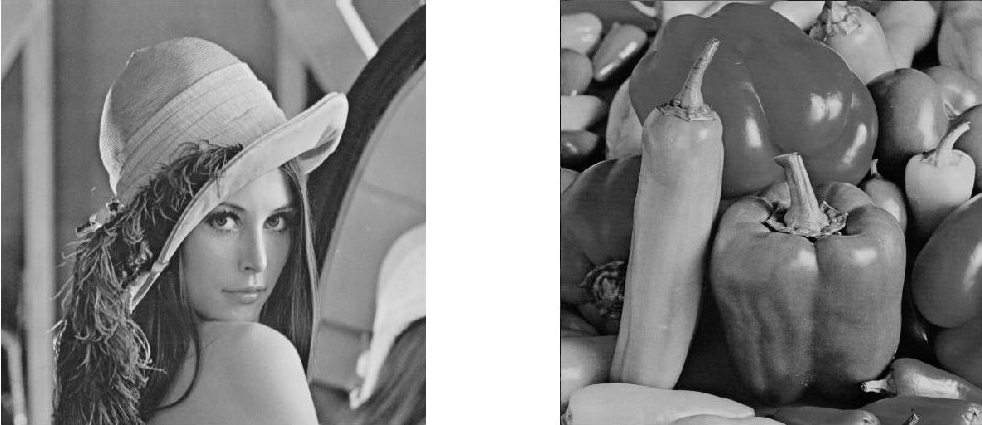
\includegraphics[width=21pc]{gfx/LennaPeppers}\caption[Im�genes de ejemplo:\\\emph{Muestra las dos im�genes de ejemplo utilizadas para mostrar el funcionamiento de \textsc{LIP}.}]{Muestra de las dos im�genes de ejemplo.}\label{fig:ejemplos}
\end{SCfigure}
\begin{SCfigure}[][!t]
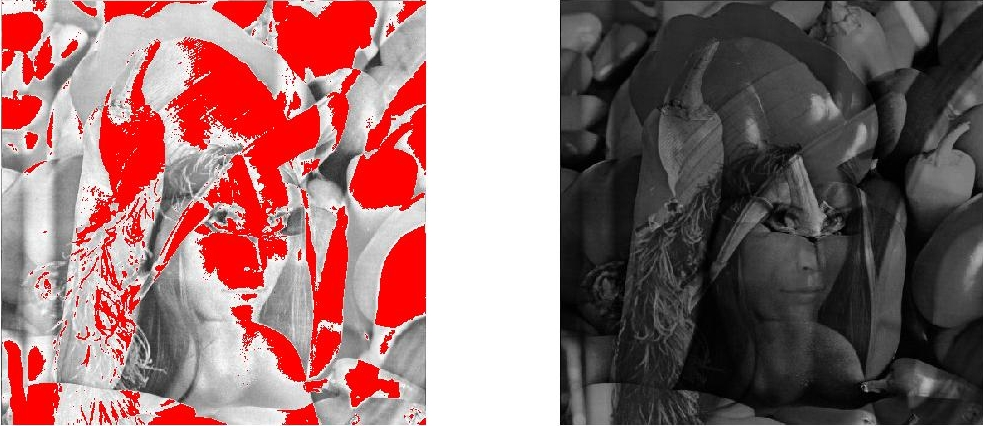
\includegraphics[width=21pc]{gfx/sumaLennaPeppers}\caption[Suma de dos im�genes: \emph{Comparaci�n de la operaci�n suma de dos im�genes entre la suma est�ndar y la suma \textsc{LIP}.}]{Suma de dos im�genes. Izquierda, suma est�ndar. Derecha, suma LIP. En rojo, todos los p��xeles que se encuentran fuera de rango.}\label{fig:suma2Img}
\end{SCfigure}
\begin{SCfigure}[][!t]
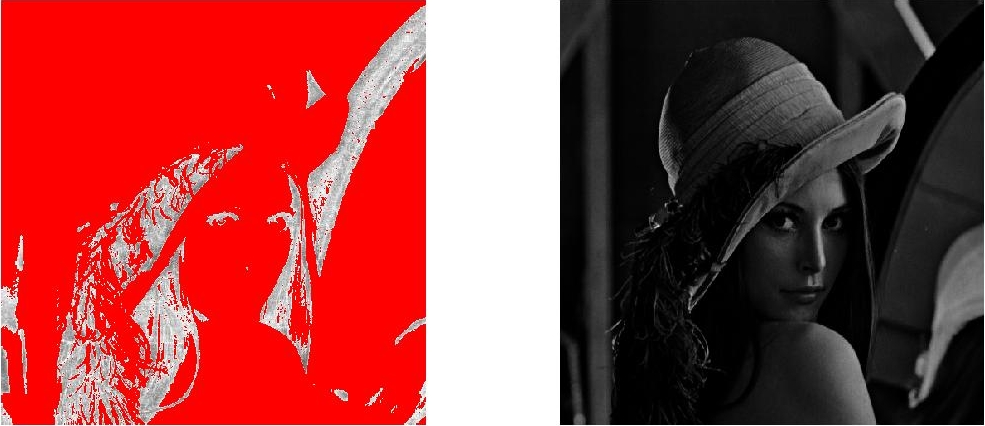
\includegraphics[width=21pc]{gfx/mult4Lenna}\caption[Multiplicaci�n escalar por 4: \emph{Comparaci�n de la operaci�n multiplicaci�n escalar de una imagen por el valor 4, utilizando la multiplicaci�n est�ndar y la multiplicaci�n \textsc{LIP}.}]{Multiplicaci�n escalar de una im�gen por 4. Izquierda, multiplicaci�n est�ndar. Derecha, multiplicaci�n LIP. En rojo, todos los p��xeles que se encuentran fuera de rango.}\label{fig:mult4LIP}
\end{SCfigure}\\[-0.5em]
\noindent Este operador garantiza que la suma de dos \emph{tonos de gris} cualesquiera ser�, a su vez, otro \emph{tono de gris} (y por tanto, se puede asegurar que el resultado se mantendr� dentro de rango). La demostraci�n matem�tica de esta propiedad se muestra en el Ap�ndice \ref{chap:apendiceA}. Visualmente, se puede apreciar el resultado de esta operaci�n en la Fig. \ref{fig:suma2Img}, en la que se muestra la suma de las dos im�genes de la Fig. \ref{fig:ejemplos}, tanto en su versi�n est�ndar como en su versi�n \textsc{LIP}. Como se muestra en la imagen de la izquierda de la Fig. \ref{fig:suma2Img}, existen muchos p��xeles cuyo valor est� fuera de rango (se�alados en rojo), mientras que en la imagen de la derecha de la Fig. \ref{fig:suma2Img}, todos los p��xeles contienen valores dentro de rango.
\item Un operador que implementa una multiplicaci�n modificada de un \emph{tono de gris} por un escalar, $\LIPtimes$, definida por:
\begin{equation}
\alpha \LIPtimes \widehat{f}=M-M\cdot\left(1-\frac{\widehat{f}}{M}\right)^\alpha \label{eq:LIPtimes}
\end{equation}

\noindent Este operador garantiza que la multiplicaci�n de un escalar por un \emph{tono de gris} es otro \emph{tono de gris}, es decir, el resultado est� definido dentro del mismo rango de funcionamiento. La demostraci�n de esta propiedad que presenta este operador se muestra en el Ap�ndice \ref{chap:apendiceB}. En la Fig. \ref{fig:mult4LIP} se muestra el resultado de la multiplicaci�n de una de las im�genes de ejemplo de la Fig. \ref{fig:ejemplos} por $4$. En la multiplicaci�n ``cl�sica'' (imagen izquierda de la Fig. \ref{fig:mult4LIP}), muchos p��xeles de la imagen resultado se han desbordado y poseen valores fuera de rango, mientras que en la imagen resultado de la multiplicaci�n \textsc{LIP} (imagen derecha de la Fig. \ref{fig:mult4LIP}) no hay ning�n p��xel con valor fuera de rango.
\item Finalmente, para extender la estructura algebraica que proporcionan $\left( \mathbb{G}^{+}, \LIPplus \ , \LIPtimes\right)$ a un espacio vectorial, se define de manera matem�tica el inverso de un \emph{tono de gris}, es decir, se define la parte negativa de $\mathbb{G}^{+}$, que se notar� como $\mathbb{G}^{-}$. Se implementa un nuevo operador, $\LIPminus$ que define la resta de dos \emph{tonos de gris} como:
\begin{equation}
\widehat{f}\LIPminus \widehat{g} = M\cdot\frac{\widehat{f}-\widehat{g}}{M-\widehat{g}}\label{eq:lipminus}
\end{equation}
\noindent Partiendo de la idea expresada en la Sec. \ref{sec:introLIP} en la que, en el modelo \textsc{LIP}, el concepto de brillo de un punto de una imagen se define como la cantidad de luz que permite pasar un \emph{filtro lum��nico} con un cierto grado de opacidad en dicho punto. Tomando el $0$ como el m�ximo nivel de iluminaci�n posible (debido a la inversi�n del rango de los \emph{tonos de gris} indicado en el primer item), los \emph{tonos de gris} $\widehat{f} \in \mathbb{G}^{-}$ no tienen significado asociado en el mundo real. Puesto que una \emph{funci�n de tonos de gris} negativa, significar��a que hay un punto en el filtro que no s�lo no es opaco y por tanto, no reduce la cantidad de luz incidente que permite pasar, sino que incrementa la iluminaci�n del punto, pudiendo incluso ser m�s brillante que el valor m�ximo posible.
\end{itemize}
\noindent Gracias a este nuevo conjunto, $\mathbb{G} = \mathbb{G}^{+} \cup\ \mathbb{G}^{-}$, se puede definir un espacio vectorial compuesto por $\left(\mathbb{G}, \LIPplus \ , \LIPtimes \ , \LIPminus\right)$.\\
%\clearpage
\noindent Utilizando los operadores descritos, se han propuesto otros \citep{pinoli97,pinoli97b,deng98}. En este trabajo se utilizar� el \mbox{\emph{Sumatorio--LIP}}, que fue dise�ado partiendo de la \emph{Suma--LIP} especificada con anterioridad:
\begin{equation}
\LIPsum{i=1}{n} \widehat{f_i} = \widehat{f_1} \LIPplus \widehat{f_2} \LIPplus \ldots \LIPplus \widehat{f_n}
\end{equation}

\subsubsection{M�todo mediante la ``Transformada'': Im�genes ``Transformadas'' y operadores ``tradicionales''}
La segunda opci�n es transformar las im�genes, trabajar utilizando los operadores ``tradicionales'', y finalmente, restaurar la imagen resultante al espacio original mediante la inversa de la transformada inicial.\\
La transformada se realiza mediante una funci�n llamada \emph{transformada isom�rfica} que se define como:
\begin{equation}
\tilde{f}=\varphi(\widehat{f}) = -M\cdot\ln\left(1-\frac{\widehat{f}}{M}\right) \label{eq:isomorTransf}
\end{equation}
La inversa de la funci�n de transformaci�n se denomina \emph{transformada isom�rfica inversa} y se define como:
\begin{equation}
\widehat{f}=\varphi^{-1}(\tilde{f}) = M\cdot\left(1-e^{-\frac{\tilde{f}}{M}}\right) \label{eq:inverseIsomorTransf}
\end{equation}
\subsection{Relaci�n con otros modelos logar��tmicos}
Existen otros paradigmas, definidos con anterioridad a \textsc{LIP}, que resuelven el problema de las operaciones fuera de rango, como por ejemplo el modelo \textsc{MHIP} \citep{oppenheim68,oppenheim69}, descrito brevemente con anterioridad en la Sec. \ref{sec:filtradoHomomorfico}, o \definicion[0.1em]{\textsc{LRIP}}{Del ingl�s, \textsc{Log--Ratio Image Processing}, procesamiento de im�genes de raz�n logar�tmica.} \citep{shvayster87,shvayster83}. Estos tres paradigmas han sido comparados \citep{pinoli97} desde tres puntos de vista diferentes: seg�n la estructura matem�tica sobre la que se han construido, seg�n la relaci�n de cada modelo con las leyes f��sicas o psico--f��sicas que los justifican, y finalmente, en funci�n del coste computacional de su desarrollo.\\
El estudio muestra que los tres modelos poseen una base matem�tica de �lgebra lineal. En ese aspecto, tanto \textsc{MHIP} como \textsc{LRIP}, poseen estructuras algebraicas basadas �nicamente en espacios vectoriales, con ordenaci�n mediante la estructura de norma. Por otra parte, \textsc{LIP} est� basado en una estructura algebraica de \emph{cono lineal con topolog��a ordenada positiva} (ver \textsc{cono lineal positivo} al pie de p�gina), al cual se le proporciona el opuesto, obteni�ndose un espacio vectorial completo. Esta estructura algebraica tan robusta proporciona un significado matem�tico a los conceptos f��sicos usados en las im�genes. Por tanto, se pueden definir los operadores siguiendo el sentido de una estructura de orden, que desde un punto de vista estrictamente algebraico produce operadores mucho m�s robustos que los obtenidos seguiendo una estructura de norma, tal y como ocurre en los modelos \textsc{MHIP} y \textsc{LRIP}.\\
\noindent En el citado art��culo \citep{pinoli97}, se demuestra que \textsc{LRIP} no sigue de forma rigurosa ninguna ley f��sica o psico--f��sica; y aunque \textsc{MHIP} s�� est� fundado en varias leyes f��sicas y/o psico--f��sicas, cumple un menor n�mero de leyes que \textsc{LIP}. En la secci�n \ref{sec:leyesLIP} se muestra un resumen de las principales leyes f��sicas y psico--f��sicas que cumple el paradigma \textsc{LIP}. Por lo tanto, \textsc{LIP} se puede afirmar que es el modelo m�s general de los tres, puesto que est� definido matem�ticamente siguiendo estructuras m�s generales, permite su aplicaci�n no s�lo a im�genes sino a cualquier funci�n matem�tica y cumple una mayor cantidad de leyes f��sicas y psico--f��sicas de construcci�n de im�genes.\\
\noindent Finalmente, con respecto al aspecto computacional, tanto \textsc{MHIP} como \textsc{LRIP} son dos modelos que trabajan utilizando ``transformadas'' (es decir, los algoritmos aplican inicialmente una funci�n de transformaci�n sobre la imagen, tras lo que realizan un procesamiento cl�sico sobre la imagen transformada y finalmente aplican la transformaci�n inversa sobre la imagen resultante). Sin embargo, \textsc{LIP} es un modelo que permite una filosof��a de trabajo tanto de tipo ``directo'' (los algoritmos cl�sicos\hfill se\hfill pueden\hfill programar\hfill usando\hfill operadores\hfill modificados 
\vfill
{\hspace{-3em} % p�gina par {-9em}
%\setlength{\tabcolsep}{1em}
\begin{tabular*}{\paperwidth}{DC}
Cono Lineal & \em Se dice que un subconjunto $C$ de un espacio vectorial $V$ es un cono lineal, si y solo si $\lambda x \in C,\ \forall x \in C, \forall \lambda \in V$.\\
Cono Lineal con Topolog��a & \em Se dice que $C$ es un cono lineal con topolog��a, si $C$ es un cono lineal y si se cumple que $a \ge b$ entonces $a+c \ge b+c$, y tambi�n, $c+a \ge c+b$, $\forall a,b,c \in C$.\\
Cono Lineal Positivo & \em Sea $C$ un cono lineal con topolog��a. Se puede obtener el cono lineal con topolog��a ordenada positiva, denominado de manera abreviada, cono lineal positivo $C^{+} \subseteq C$, tomando el conjunto de valores $a \in C$ que cumplen que $a \ge 0$.\\
\end{tabular*}}
\clearpage
\noindent que proporcionan directamente una imagen resultante, sin necesidad de aplicar ninguna transformada) como de tipo ``transformada'', lo que hace que muchos algoritmos se puedan implementar utilizando, al menos, dos mecanismos diferentes.
\subsection{Leyes f��sicas y psico--f��sicas que cumple \textsc{LIP}}\label{sec:leyesLIP}
Como se ha indicado con anterioridad, adem�s de tener una base algebraica robusta, \textsc{LIP} no es una mera invenci�n matem�tica, sino que tiene un sustento en la forma en la que el sistema visual humano percibe las escenas. En el modelo \textsc{LIP}, el brillo de un punto de una imagen se ha demostrado que es la cantidad de luz que pasa por un filtro lum��nico con una determinada funci�n de absorci�n. Se ha demostrado \citep{pinoli97,pinoli97b} que \textsc{LIP} cumple una serie de leyes f��sicas y de leyes psico--f��sicas ampliamente aceptadas dentro de la comunidad cient��fica, entre las que cabe destacar las siguientes:
\subsubsection{Inversi�n de escala de tonos de gris}\label{sec:leyesLIP:Inversion}
Los l��mites del intervalo $(0,M)$ representan, respectivamente, el ``umbral superior'' (tambi�n conocido como \emph{l��mite de deslumbramiento}) y el ``umbral inferior'' (o \emph{l��mite de oscuridad total}). El \emph{l��mite de deslumbramiento} se corresponde con el valor superior de iluminaci�n que el ojo humano es capaz de soportar y distinguir, debido a la intensidad m�xima con la que responden los fotorreceptores de la retina humana. Cualquier incremento de la intensidad lum�nica por encima de dicho valor no se traduce en un aumento de la respuesta de los fotorreceptores, porque dichos fotorreceptores se encuentran funcionando al l�mite m�ximo. Por el contrario, al alcanzar el \emph{l�mite de oscuridad total}, el sistema visual humano mostrar�a una ausencia completa de respuesta. Sin embargo, este umbral de oscuridad es un l�mite te�rico inalcanzable, puesto que est� demostrado \citep{zuidema83,baylor84} que el ojo humano muestra sensibilidad a una baja cantidad de fotones. Esto se puede probar cerrando los ojos en una habitaci�n oscura y notando como ``aparecen'' peque�os destellos en la imagen observada, similares al ruido gaussiano. Es decir, que el sistema visual humano proporciona repuesta ante una presencia �nfima de fotones, mostrando que incluso ante una oscuridad plena, el sistema visual humano tiene cierto nivel de sensibilidad, demostrando emp�ricamente que el \emph{l�mite de oscuridad total} no es alcanzable en condiciones naturales por el sistema visual humano.\\
La inversi�n de escala se justifica de dos maneras. La primera, en el �mbito de los procesos de formaci�n de im�genes por luz transmitida, donde las \emph{funciones de tonos de gris} se deben tomar como filtros de transparencia, de manera que el valor $0$ se ha de tomar como \emph{transparencia total}, disminuyendo el grado de transparencia conforme aumenta el valor, hasta tomar el valor de \emph{opacidad total} ($M$). En segundo lugar, tambi�n tiene validez desde el punto de vista de la percepci�n visual humana. De hecho, se ha demostrado a trav�s de experimentos psicof��sicos \citep{baylor84} utilizando monos (que poseen un sistema visual con muchas semejanzas con el sistema visual humano) que en una ausencia completa de est�mulos luminosos (simulando una te�rica ``oscuridad plena''), la intensidad bio--el�ctrica de la retina es constante a un valor no nulo y que el aumento de la iluminaci�n en la recepci�n se traduce en una reducci�n de dicho nivel de intensidad bio--el�ctrica y no en un aumento como cabr��a esperar. Por tanto, para garantizar la inversi�n de escala, \textsc{LIP} hace uso de \emph{funciones de tono de gris} en lugar de im�genes en el rango habitual. Gracias a esta inversi�n, el modelo \textsc{LIP} trabaja de manera similar y consistente a como lo hace el sistema visual humano.
\subsubsection{Relaci�n de los tonos de gris con la Intensidad Lum��nica}
En el contexto de la percepci�n visual humana, una \emph{funci�n de tono de gris} $\widehat{f}$ se relaciona con el valor de la funci�n de intensidad de la luz incidente $F$ mediante:
\begin{equation}
\widehat{f}=M\left(1-\frac{F}{F_{\max}}\right) \label{eq:relacionTonoGrisconIntensidad}
\end{equation}
donde $F_{\max}$ es el \emph{umbral superior} o \emph{l��mite de deslumbramiento} del sistema visual humano, anteriormente citado.\\
Utilizando \eqref{eq:relacionTonoGrisconIntensidad}, \textsc{LIP} permite relacionar un concepto f�sico, la funci�n de intensidad de la luz incidente, $F$, con una definici�n propia del funcionamiento de \textsc{LIP}, como es la \emph{funci�n de tono de gris}, $\widehat{f}$, que se corresponde con una funci�n de intensidad de luz incidente valuada en el rango del intervalo real $(0,F_{\max}]$, donde $F_{\max}<M$. De hecho, la definici�n de un \emph{tono de gris} en el contexto de la percepci�n humana de la intensidad lum�nica se puede considerar que es una funci�n normalizada con inversi�n de escala.
\subsubsection{Saturaci�n Lum��nica}
Al contrario que otros paradigmas, que no est�n limitados en el rango de intensidades, \textsc{LIP} propone un rango limitado $(0,M)$, que es consistente con el principio de saturaci�n lum��nica del sistema visual humano, en el cual, m�s all� de un cierto l��mite ($F_{\max}<M$), el ojo humano no es capaz de reconocer ning�n aumento posterior en la cantidad de intensidad de luz incidente.
\subsubsection{Ley de Weber}
Desde mediados del siglo \textsc{XIX} se sabe que la respuesta del sistema visual humano a la intensidad lum��nica no es lineal. Fue Weber el que expuso una ley en la que defend��a que el sistema de detecci�n visual humana depende del cociente de la divisi�n de los valores de intensidad lum�nica m�s que de la diferencia entre los diversos valores de intensidad. De hecho, introdujo el concepto de ``\emph{diferencia de iluminaci�n m��nima distinguible}'', que es la cantidad de luz necesaria que hay que sumar a un campo de prueba con valor lum��nico, $F$, para que sea visualmente apreciable la diferencia con otro campo de prueba fijo a un valor lum��nico $F$. La ley de Weber se describe:
\begin{equation}
\frac{\Delta F}{F}=W
\end{equation}
donde $W$ es una constante, llamada \emph{Constante de Weber}.\\%Sean $F$ y $G$, dos valores de intensidad lum�nica en un punto y, $\widehat{f}$ y $\widehat{g}$, sus tonos de gris asociados. La resta \textsc{LIP} de ambos, utilizando las Ec. \ref{eq:lipminus} y \ref{eq:relacionTonoGrisconIntensidad}, se define como:
% \begin{equation}
% \widehat{g}\LIPminus \widehat{f} = M\frac{\widehat{g}-\widehat{f}}{M-\widehat{f}}=M\frac{F-G}{F}
% \end{equation}
% Si se asume que $F$ y $G$ presentan intensidades lum�nicas ``m��nimamente distinguibles'', se puede aplicar $G = F+\Delta F$ y por tanto, la diferencia entre los tonos de gris asociados, denotada dicha diferencia como $\Delta \widehat{f}$ es:
% \begin{equation}
% \Delta \widehat{f} = \widehat{g}\LIPminus \widehat{f} = -M\frac{\Delta F}{F} = -M\cdot W
% \end{equation}

\noindent Est� demostrado \cite{pinoli97b} que la operaci�n resta \textsc{LIP} es consistente con la ley de Weber. Aunque esta ley ha sido muy criticada debido a que s�lamente se cumple para valores de intensidad de luz superiores a un cierto nivel, y a que la constante de Weber s�lo es v�lida dependiendo del tama�o del elemento a detectar. A pesar de todo ello, el modelo \textsc{LIP} es plenamente v�lido dentro del campo de modelizaci�n de la percepci�n visual humana, ya que en todas las situaciones donde sea cierta la ley de Weber, la resta \textsc{LIP} expresa correcta y coherentemente dicha ley.
\subsubsection{Ley de Fechner}
Unos a�os despu�s que Weber, Fechner explic� la no--linealidad del sistema de percepci�n visual humano de la siguiente manera:
\begin{quote}
{\em Para producir pasos aritm�ticos incrementales en la sensaci�n visual, la intensidad lum��nica habr� de crecer geom�tricamente.}\end{quote}
\noindent As�� pues, introdujo una relaci�n entre la intensidad lum��nica en un punto, $F$, tomado como est��mulo de entrada y el brillo observado en dicho punto, $B$, que representa la sensaci�n visual percibida por el ojo humano en dicho punto. Esta relaci�n di� lugar a la \emph{Ley Discreta de Fechner}:
\begin{equation}
\Delta B = k\frac{\Delta F}{F}
\end{equation}
donde $\Delta F$ es el incremento de luz que produce un incremento de la sensaci�n de brillo ($\Delta B$) y siendo $k$ una constante. La \emph{Ley Cont��nua de Fechner} se puede expresar como:
\begin{equation}
B= k'\ln\left(\frac{F}{F_{\min}}\right)
\end{equation}
donde $k'$ es una constante y $F_{\min}$ es el \emph{umbral de funcionamiento absoluto} del ojo humano que representa el valor de iluminaci�n m�nima a partir del cual comienzan a distinguirse cambios de iluminaci�n y que se sabe que es muy cercano a la descripci�n f��sica de oscuridad absoluta. La ley de Fechner se puede escribir tambi�n como:
\begin{equation}
B=k'\ln\left(\frac{F}{F_{\max}}\right)+k'\ln\left(\frac{F_{\max}}{F_{\min}}\right)\label{eq:fechner-continua}
\end{equation}
donde $F_{\max}$ es el \emph{umbral superior} o \emph{l��mite de deslumbramiento} del sistema visual humano, anteriormente citado.\\
La resta \textsc{LIP} se muestra consistente con la \emph{Ley Discreta de Fechner} y con la \emph{Ley Cont��nua de Fechner}, puesto que aplicando el isomorfismo $\varphi$ del modelo \textsc{LIP} sobre \eqref{eq:fechner-continua} se obtiene \eqref{eq:fechner-LIP}, que demuestra la relaci�n.
\begin{equation}
B=-\frac{k'}{M}\varphi(\widehat{f})+k'\ln\left(\frac{F_{\max}}{F_{\min}}\right)\label{eq:fechner-LIP}
\end{equation}
De hecho, la ley de Fechner fue uno de los primeros intentos de encontrar una escala lineal para el brillo o sensaci�n de intensidad lum��nica con las operaciones cl�sicas de suma y multiplicaci�n, mientras que \textsc{LIP} define operaciones espec��ficas que trabajan directamente con la funci�n de intensidad lum��nica (est��mulo de entrada).
\section{Modelos de ruido en im�genes}
\lettrine{L}{a} tecnolog��a de captaci�n de im�genes por medios digitales est� en un continuo avance. Los sensores admiten una mayor resoluci�n y tienen un comportamiento cada vez m�s real��stico. Sin embargo, la captaci�n de im�genes no es precisa y hay una cierta probabilidad de introducir ruido en la imagen digitalizada. Este ruido se puede definir como la alteraci�n apreciable en el valor de un p��xel digital determinado con respecto al valor de intensidad asociado a la posici�n de dicho punto en la imagen real. Se ha estudiado ampliamente el ruido en las im�genes y se han propuesto diversos mecanismos para eliminar completamente (en los casos que sea posible) o, al menos, mitigar el efecto de dicho ruido.
\subsection{Ruido en im�genes}
Inicialmente, se debe precisar qu� es lo que se entiende por ruido dentro del �mbito del \textsc{Procesamiento de Im�genes}. En \person{Bovik \etal} \citep{bovik00}, el ruido se define como \emph{una componente no deseada de la imagen digitalizada}. Sin embargo, esta definici�n es demasiado amplia y se puede concretar m�s indicando que:\\[1em]
\begin{tabular}{|A|}
\hline
Se define el \emph{ruido} en las im�genes como toda alteraci�n no deseada en la imagen digitalizada que hace que �sta sea diferente de la imagen real original.\vspace{1em}\\
\hline
\end{tabular}\\[1em]
\noindent La mayor��a de las veces dichas alteraciones son apreciables para el observador, pero otras son peque�as modificaciones del valor digitalizado de los p��xeles que apenas son detectables para el sistema visual humano. Desde el punto de vista matem�tico, las alteraciones sufridas por un p��xel en particular pueden provenir de una modificaci�n del valor del p��xel ``real'' elevando o disminuyendo su valor linealmente. As�� pues, una imagen con ruido se puede modelar \citep{gonzalez02} como:
\begin{equation}
g(x,y) = h(x,y) \ast f(x,y) + \eta(x,y),
\end{equation}
\noindent donde $f(x,y)$ es la imagen original, $g(x,y)$ es la imagen original alterada con ruido, $h(x,y)$ es una funci�n de degradaci�n que se aplica espacialmente mediante el operador convoluci�n y $\eta(x,y)$ es un cierto ruido \emph{aditivo} no dependiente de la imagen original. La funci�n $h(x,y)$ tambi�n es llamada ruido \emph{multiplicativo}.\\
\noindent Existen una variedad de modelos de ruido, la mayor��a de ellos de tipo aditivo. A continuaci�n se expondr�n brevemente dos de los m�s habituales.
\paragraph{Ruido Gaussiano} \noindent El ruido aditivo m�s habitual es el gaussiano. Se utiliza para modelar el ruido termal y, bajo algunas ligeras restricciones asumibles, el ruido por conteo de fotones y el ruido por la granularidad de la pel��cula fotogr�fica. Este tipo de ruido se basa en que la probabilidad de que un p��xel se modifique se reduce siguiendo una distribuci�n de probabilidad gaussiana conforme aumenta la diferencia entre el valor de la variaci�n que sufre dicho p��xel y el valor real del mismo. Es decir, la probabilidad de que un p��xel no sufra variaci�n alguna es elevada, y la probabilidad de que un p��xel tenga una variaci�n extrema es muy poco probable. La funci�n de densidad que determina la probabilidad de ruido gaussiano univariado (con media $\mu$ y varianza $\sigma^2$) es:
\begin{equation}
P(x)=\frac{1}{\sigma\sqrt{2\pi}}\cdot e^{-\frac{(x-\mu)^2}{2\sigma^2}}
\end{equation}
\noindent donde $x$ puede tomar cualquier valor del interlvalo $(-\infty, \infty)$. Como esta definici�n puede provocar la obtenci�n de valores negativos, aspecto no admisible en im�genes de intensidad, en la pr�ctica el rango de valores de ruido gaussiano se limita a aproximadamente $\pm 3\sigma$, truncando aquellos valores que el ruido gaussiano pudiese llevar a obtener valores negativos \citep{bovik00}.\\
\noindent El ruido gaussiano es muy utilizado para modelar el comportamiento del ruido en las im�genes debido al propio proceso de captaci�n de las mismas. Las im�genes son captadas por sensores \definicion{CCD}{Del ingl�s, \textsc{Charge--Coupled Device}, dispositivo de carga acoplada.} que miden la energ��a termal producida por el choque de los electrones incidentes en cada elemento del sensor. Los sensores \textsc{CCD} suponen que la mayor��a de los electrones que captan provienen de la luz incidente, sin embargo, existen una cantidad de electrones provenientes del propio material del \textsc{CCD} que, por excitaci�n termal, pueden incidir en el valor captado. Resumiedo, el ruido termal cumple tres caracter��sticas: es el resultado de la vibraci�n de una gran cantidad de electrones, la vibraci�n de cada electr�n es independiente de la de los dem�s y, finalmente, no existen electrones que provoquen una contribuci�n significativa mayor que la de los dem�s. Estas tres condiciones (f�cilmente asumibles) hacen que este ruido se pueda modelar como una distribuci�n de probabilidad Gaussiana, gracias al Teorema del L��mite Central \citep{gallego01}. Es decir, el valor captado por cada sensor \textsc{CCD} se puede desviar ligeramente del valor real debido a la presencia de esos electrones excitados por vibraci�n termal; es muy probable que la variaci�n sea nula o muy cercana a cero y es muy poco probable que dicha variaci�n sea muy grande.
\paragraph{Ruido de ``sal y pimienta''} \noindent Este tipo de ruido \graffito{El ruido de ``sal y pimienta'' presenta puntos blancos y negros de manera dispersa.} produce una degradaci�n muy caracter��stica en la imagen: s�lo hay unos pocos p��xeles ruidosos, pero la variaci�n (el ruido) que presentan es extrema (tanto hacia el blanco como hacia el negro). Este tipo de ruido aparece t��picamente en la transmisi�n de im�genes por canales digitales con muchas interferencias. En estos casos, cada bit se transmite de manera independiente a los dem�s, por lo que el cambio de valor de uno de los bits m�s significativos provoca que cambie completamente su valor debido a una mala decodificaci�n.
\subsection{Emborronamiento de im�genes}
Por la propia naturaleza del ruido, en una primera aproximaci�n se determina que �ste se concentra en puntos m�s o menos aislados, en los que se produce un ``salto'' en los valores de la intensidad con respecto a los valores de los p��xeles cercanos. Esto hace que el ruido modifique el espectro de la imagen en las altas frecuencias. Debido a esta caracter��stica, la primera soluci�n que se suele plantear ante la presencia de ruido es la aplicaci�n de un operador de filtrado paso baja, para eliminar las componentes de altas frecuencias presentes en el ruido. Este filtro no deber��a ser demasiado severo, puesto que podr��a eliminar completamente la estructura de la imagen, ya que, como se ha comentado anteriormente, la \emph{reflectancia}, que contiene la estructura de los objetos, tambi�n se concentra principalmente en las altas frecuencias. En general, al aplicar un filtro paso baja se produce un cierto emborronamiento de las im�genes, mediante el cual se suele eliminar o mitigar el efecto local del ruido en la imagen, difuminando el efecto entre los p��xeles de un entorno.\\
\noindent Para realizar el filtrado paso baja en el dominio espacial es habitual la utilizaci�n del operador convoluci�n con m�scaras m�s o menos extensas. Uno de los filtros paso baja m�s simples es el \emph{filtrado por la media} de entorno $X\times Y$, es decir, el valor de un p��xel viene dado por la media de los valores del entorno de dicho p��xel (incluyendo o no al p��xel en consideraci�n).\\
\noindent Existe otro conjunto de filtros paso baja m�s complejos, que son los basados en la distribuci�n de probabilidad estad��stica del ruido. El ruido es una alteraci�n en la medida de un valor y est� ampliamente aceptado que la variaci�n en la medici�n de un valor sigue una distribuci�n estad��stica de tipo Gaussiana. Tambi�n se ha estudiado \citep{canny86} que un p��xel no es una variable estad��stica independiente y que no todo el entorno de un p��xel afecta por igual al valor del punto en consideraci�n. Los p��xeles m�s cercanos afectan o influyen m�s que los m�s lejanos. Si se supone que el ruido sigue una distribuci�n estad��stica de tipo Gaussiana, el filtrado de la imagen con una m�scara Gaussiana permite que este filtrado afecte de manera controlada a los bordes reales de los objetos. El control de esta operaci�n viene dado por la varianza de la distribuci�n Gaussiana, que permite tener un filtro m�s amplio, m�s estrecho, etc., lo que permite modificar el conjunto de p��xeles al que afecta la m�scara Gaussiana. A esta operaci�n se le suele denominar \emph{filtrado Gaussiano} de varianza $\sigma$.
\section{Extracci�n de bordes}
\lettrine{U}{na} de las operaciones fundamentales del procesamiento de im�genes es la detecci�n de bordes, por lo que es un procedimiento muy com�n en el procesamiento de im�genes est�ticas. Los bordes suelen coincidir con los l��mites de los objetos presentes en las im�genes, aunque tambi�n pueden presentarse bordes internos a los objetos, en el fondo, o justo lo contrario, que no se muestre el borde de un objeto porque el cambio de la intensidad de la imagen en el borde no sea abrupto, sino muy gradual, y por lo tanto no se detecte. De manera gen�rica, existe una gran correlaci�n entre los bordes f��sicos de los objetos y los bordes representados en las im�genes. Sin embargo, existen casos en los que se pueden marcar como bordes en las im�genes p��xeles que no corresponden con ning�n objeto f��sico, como es el caso de las sombras proyectadas.\\
\noindent De las tres grandes familias de operadores que extraen los bordes en las im�genes, Operadores basados en el Gradiente, Operadores basados en el Laplaciano y Operadores Morfol�gicos, a continuaci�n s�lo se introducen las dos primeras, ya que los Operadores Morfol�gicos no est�n relacionados con el trabajo desarollado en esta Tesis.
\vspace{-0.9em}\subsection{Filtros basados en el gradiente de la imagen}
\vspace{-0.5em}De manera gen�rica y, por simplificaci�n, aplicado sobre im�genes en tonos de gris, se define un borde como la localizaci�n espacial de un cambio abrupto en valores de tonos de gris espacialmente cercanos. Esta afirmaci�n se puede extender indicando que un \emph{borde se define como la localizaci�n espacial donde se da un m�ximo o un m��nimo en la derivada de la funci�n tono de gris, tambi�n llamado \textsc{gradiente} de la imagen}. En concreto, lo que se busca son los m�ximos en la funci�n valor absoluto del gradiente de la imagen, es decir:
\begin{equation}
\left|\nabla f(x,y)\right| \geq T,
\end{equation}
\noindent donde $T$ representa el umbral de detecci�n.\\

\noindent Una vez que se obtiene la imagen formada por aquellos p��xeles cuyo gradiente es mayor que el umbral $T$, se suele aplicar un proceso de disminuci�n o adelgazamiento de los m�ximos detectados, puesto que los extremos detectados suelen estar rodeados de valores altos que superan el umbral establecido y s�lo interesan los valores m�ximos locales de cada entorno detectado en la direcci�n del gradiente.\\
\noindent En general, las aproximaciones al c�lculo de la funci�n gradiente en un espacio discreto, como es el de las im�genes digitales, se suele realizar mediante un par de filtros orientados ortogonalmente, $h_1(x,y)$ y $h_2(x,y)$. Estos se convolucionan de manera independiente sobre la imagen, de manera que la suma del resultado de ambos es la aproximaci�n a la imagen gradiente:
\begin{equation}
\widehat{\nabla} f(x,y) = \left(f(x,y)\ast h_1(x,y)\right) \cdot \vec{u_1} + \left(f(x,y)\ast h_2(x,y)\right) \cdot \vec{u_2}
\end{equation}
\noindent donde $\vec{u_1}$ es un vector unitario en la direcci�n del filtro $h_1$ y $\vec{u_2}$ es un vector unitario en la direcci�n del filtro $h_2$.
\paragraph{Detectores Simples de Bordes Horizontales y Verticales} \noindent A veces se desea extraer �nicamente bordes horizontales o verticales. Para ello, se convoluciona la imagen con filtros que responden s�lo en dichas direcciones. Estos filtros pueden usar diferencias entre p��xeles a distancia uno o diferencias centrales, que respectivamente son:
\begin{eqnarray}
h_1(x,y) =
\begin{bmatrix}
     0 & 0\\
    \circledtwochars{-1} & 1
\end{bmatrix} && h_2(x,y) =
\begin{bmatrix}
     1 & 0\\
    \circledtwochars{-1} & 0
\end{bmatrix}
\\
h_1(x,y) =
\begin{bmatrix}
     0 & 0 & 0\\
    -1 & \circled{0} & 1\\
     0 & 0 & 0
\end{bmatrix} && h_2(x,y) =
\begin{bmatrix}
     0 & 1 & 0\\
     0 & \circled{0} & 0\\
     0 &-1 & 0
\end{bmatrix}
\end{eqnarray}
\noindent Se ha resaltado la posici�n central $(x,y)$ sobre la que se aplica el filtro en la imagen.\\
\noindent Todos los filtros que se propongan han de sumar $0$ en sus componentes, ya que implementan una derivada y no deben dar una respuesta ante una constante.
\paragraph{Filtro de Roberts para bordes Diagonales}\noindent El filtro para la detecci�n de bordes de Roberts \citep{roberts65} est� indicado para la detecci�n de bordes diagonales:
\begin{equation}
h_1(x,y) = \begin{bmatrix}
    0 & 1\\
    \circledtwochars{-1}&0
\end{bmatrix}
\qquad h_2(x,y) = \begin{bmatrix}
    1 & 0\\
    0&\circledtwochars{-1}
\end{bmatrix}
\end{equation}
\noindent Este operador presenta un par de problemas. El primero es que el punto de cruce de la diagonal $[-1\ 1]$ se localiza entre p��xeles, es decir, que no coincide con ninguna posici�n real en la estructura en rejilla de los p��xeles. Sin embargo, como es necesario asignar dicho punto de cruce a alguna localizaci�n, se producen errores de aproximaci�n generalizados. El segundo problema que presenta este operador (y en general todos aquellos que usan s�lo informaci�n de dos p��xeles) es que su sensibilidad al ruido es bastante alta.
\paragraph{Filtro de Prewitt}\noindent Una posible soluci�n para evitar el primero de los problemas que presenta el filtro anterior es dise�ar los filtros en base a las diferencias centrales, para lo cual se utiliza habitualmente un entorno de $3\times3$ p��xeles. Para evitar el segundo de los problemas se suele aplicar un suavizado, que lo que hace es incorporar m�s p��xeles en el proceso de c�mputo del valor del p��xel central, dando el resultado en funci�n de los p��xeles de su entorno, no s�lo de 2 p��xeles.\\
\noindent Teniendo en cuenta esto, para obtener los filtros de Prewitt \citep{prewitt70} se definen dos funciones, $h_x(x)$ y $h_y(y)$, que dependen, respectivamente, s�lo de $x$ e $y$. Mediante el producto escalar de estas dos funciones se obtienen unos filtros separables, ortogonales, y que adem�s aplican suavizado al resultado:
\begin{equation}
h_y(y) = \begin{bmatrix}
1&\circled{1}&1
\end{bmatrix}'  \qquad h_x(x) = \begin{bmatrix}
-1&\circled{0}&1
\end{bmatrix}
\end{equation}
\begin{eqnarray}
h_1(x,y) &=& h_y(y)\cdot h_x(x) \nonumber \\
\begin{bmatrix}
    1\\
\circled{1}\\
    1
\end{bmatrix}\cdot
\begin{bmatrix}
-1&\circled{0}&1
\end{bmatrix} &=&
\begin{bmatrix}
-1&0&1\\
-1&\circled{0}&1\\
-1&0&1
\end{bmatrix}
\end{eqnarray}
\noindent As�� pues, los filtros del operador de Prewitt son:
\begin{equation}
\begin{bmatrix}-1&0&1\\-1&\circled{0}&1\\-1&0&1\end{bmatrix} \qquad \begin{bmatrix}1&1&1\\0&\circled{0}&0\\-1&-1&-1\end{bmatrix}
\end{equation}
\paragraph{Filtro de Sobel}\noindent Propuesto por primera vez por \person{Irwin Sobel} \citep{sobel68,sobelPhD} en una charla dentro del Proyecto Stanford Artificial en 1968. Este operador se ha convertido en uno de los m�s utilizados tanto por la buena respuesta que ofrece como por su relativamente bajo coste computacional. Es una variante del operador de Prewitt, que utiliza $[1\ 2\ 1]$ en lugar de $[1\ 1\ 1]$, realizando un mejor suavizado. Por tanto, los filtros del operador de Sobel son:
\begin{equation}
\begin{bmatrix}-1&0&1\\-2&\circled{0}&2\\-1&0&1\end{bmatrix} \qquad \begin{bmatrix}1&2&1\\0&\circled{0}&0\\-1&-2&-1\end{bmatrix}\label{eq:mascarasSobelSTD}
\end{equation}
\paragraph{Filtro de Frei--Chen}\noindent El filtro de Prewitt tiene m�s sensibilidad a la detecci�n de bordes horizontales y verticales que a los bordes diagonales, mientras que el filtro de Sobel tiene m�s sensibilidad a los bordes diagonales que a los horizontales y verticales. Esto es debido a que ambos filtros se han desarrollado sin tener en cuenta la compensaci�n debida a la distancia, que es distinta entre los p��xeles diagonales y los p��xeles horizontales y verticales. Es decir, que tanto \emph{el filtro de Prewitt} como \emph{el filtro de Sobel} presentan \definicion{anisotrop��a}{Propiedad que se manifiesta de manera diferente seg�n la direcci�n estudiada.}.\\
El filtro del operador de Frei--Chen \citep{frei77} es:
\begin{equation}
\begin{bmatrix}-1&0&1\\-\sqrt{2}&\circled{0}&\sqrt{2}\\-1&0&1\end{bmatrix} \qquad \begin{bmatrix}1&\sqrt{2}&1\\0&\circled{0}&0\\-1&-\sqrt{2}&-1\end{bmatrix}
\end{equation}
\noindent Este filtro, aunque no es totalmente isotr�pico, puesto que no es rotacionalmente sim�trico, introduce una anisotrop��a reducida y aceptable.
\paragraph{Filtro de Scharr}\noindent Existen muchos procesos que exigen filtros con muy alta isotrop��a, es decir, que se comporten de manera similar sin presentar mayor sensibilidad en la direcci�n de los patrones evaluados. \person{Scharr \etAl} \citep{scharr00} presentan un filtro que tiene un comportamiento invariante y optimizado ante la rotaci�n.
\begin{equation}
\frac{1}{32}\cdot\begin{bmatrix}-3&0&3\\-10&\circled{0}&10\\-3&0&3\end{bmatrix} \qquad \frac{1}{32}\cdot\begin{bmatrix}3&10&3\\0&\circled{0}&0\\-3&-10&-3\end{bmatrix}
\end{equation}
\subsection{Filtros basados en el Laplaciano de la imagen}
El Laplaciano de una imagen $f(x,y)$ se define matem�ticamente como:
\begin{equation}
\nabla^2 f(x,y)=\nabla \cdot \nabla f(x,y) = \frac{\partial^2 f(x,y)}{\partial x^2}+\frac{\partial^2 f(x,y)}{\partial y^2}
\end{equation}
\noindent Al aplicar la segunda derivada, los bordes de la imagen producir�n ceros en esta funci�n, por lo que una de las ventajas que proporciona es que produce bordes sin grosor, puesto que es el cero en s�� el que proporciona un �nico punto de cruce, de manera que no es necesario aplicar un paso posterior de adelgazamiento de bordes. La funci�n Laplaciana (en su versi�n de funci�n continua) es isotr�pica, puesto que no favorece ninguna direcci�n en particular. Adem�s, los bordes que presenta son contornos cerrados, ya que, al no tener en cuenta la fuerza de los extremos, sino s�lo el paso por cero, el m�s peque�o cambio gradual produce un paso por cero.\\
\noindent Sin embargo, el Laplaciano presenta algunos problemas:
\begin{itemize}
\item Produce la aparici�n de bordes falsos al detectarse pasos por cero en cambios de convexidad en la funci�n de la imagen.
\item Presenta una alta sensibilidad a la presencia de errores, debido al uso de la segunda derivada, creando bordes falsos, al producirse cambios en regiones constantes, o modificando los bordes reales existentes.
\end{itemize}
\noindent El operador Laplaciano es un escalar, frente al operador gradiente que es un vector; por lo tanto, en lugar de un par de filtros ortogonales, es necesario un �nico filtro para obtener el Laplaciano.
\begin{equation}
\widehat{\nabla}^2 f(x,y) = f(x,y)\ast h(x,y) \label{eq:laplacianoGeneral}
\end{equation}
\noindent Para evitar el problema de la detecci�n de los pasos por cero entre p��xeles, en lugar de usar s�lo 2 p��xeles, se suele usar un entorno de 3 p��xeles, de tal manera que se puede obtener un operador Laplaciano de manera simple de la siguiente forma:
\begin{eqnarray}
\frac{\partial f(x,y)}{\partial x} &\rightarrow & f_x(x,y) = f(x+1,y) - f(x,y) \label{eq:derivadaX}\\
\frac{\partial^2 f(x,y)}{\partial x^2} &\rightarrow & f_{xx}(x,y) = f(x,y) - f(x-1,y) \label{eq:derivadaX2bis}\\
\nonumber \\
\frac{\partial^2 f(x,y)}{\partial x^2} &\rightarrow & f_{xx}(x,y) =\nonumber\\
 &=& f(x+1,y) -2f(x,y) + f(x-1,y) =\nonumber\\
 &=& \begin{bmatrix}1&\circledtwochars{-2}&1\end{bmatrix} \label{eq:derivadaX2}
\end{eqnarray}
\noindent Actuando de manera an�loga con $y$ se obtiene:
\begin{equation}
\frac{\partial^2 f(x,y)}{\partial y^2} \rightarrow f_{yy}(x,y) = \begin{bmatrix}1\\\circledtwochars{-2}\\1\end{bmatrix} \label{eq:derivadaY2}
\end{equation}
\noindent Al unificar \eqref{eq:laplacianoGeneral}, \eqref{eq:derivadaX2} y \eqref{eq:derivadaY2} (estas dos �ltimas extendidas a un tama�o de filtro de $3\times 3$), se puede calcular:
\begin{equation}
\widehat{\nabla}^2 f(x,y) = \begin{bmatrix}0&0&0\\1&\circledtwochars{-2}&1\\0&0&0\end{bmatrix}+\begin{bmatrix}0&1&0\\0&\circledtwochars{-2}&0\\0&1&0\end{bmatrix}=\begin{bmatrix}0&1&0\\1&\circledtwochars{-4}&1\\0&1&0\end{bmatrix}
\end{equation}
\noindent Mediante otras aproximaciones a la segunda derivada, es decir, proponiendo otras ecuaciones \eqref{eq:derivadaX} y \eqref{eq:derivadaX2bis} y utilizando este mismo m�todo, se pueden construir otros filtros Laplacianos alternativos. Dos ejemplos de filtros Laplacianos distintos del anterior son:
\begin{equation}
\begin{bmatrix}1&1&1\\1&\circledtwochars{-8}&1\\1&1&1\end{bmatrix} \qquad \begin{bmatrix}-1&2&-1\\2&\circledtwochars{-4}&2\\-1&2&-1\end{bmatrix}
\end{equation}
\subsubsection{Laplaciano de Gaussianas (LoG)}
Aunque en una imagen pueden existir muchos bordes, el ojo humano es capaz de realizar segmentaciones autom�ticas y extraer s�lo aquellos bordes que le interesan en funci�n de la tarea que se est� realizando; para detectar los objetos principales s�lo se tienen en cuenta aquellos bordes m�s abruptos, mientras que para observar la textura de un objeto hay que tener en cuenta todos sus bordes y pliegues. Esta caracter��stica ha sido altamente deseada por los cient��ficos con el objetivo de obtener un detector de bordes ajustable seg�n la sensibilidad escogida.\\
\noindent El operador Laplaciano de Gaussianas \citep{marr80}, \definicion{LoG}{Del ingl�s, \textsc{Laplacian of Gaussian}}, tambi�n conocido como operador de \emph{Marr--Hildreth}, es un operador que incorpora el concepto de control de sensibilidad. Se ha observado que la convoluci�n de una imagen con un filtro Gaussiano produce un suavizado que limita la imagen resultante a un rango espec��fico de frecuencias, amortiguando el impacto de la presencia de ruido o de bordes d�biles (y por tanto no deseados). Si sobre esta imagen filtrada se aplica el operador Laplaciano, se obtienen los pasos por cero en funci�n del grado de sensibilidad que se desee, que es un par�metro controlable por la desviaci�n t��pica ($\sigma$) de la Gaussiana aplicada como filtro.\\
\noindent La Gaussiana presenta unas propiedades que facilitan su uso como filtro del detector de bordes:
\begin{itemize}
\item La Gaussiana es una funci�n suave y claramente localizada tanto en el dominio espacial como en el dominio de las frecuencias. Esto permite un comportamiento de suavizado ante los errores a la vez que de precisi�n en la localizaci�n de los bordes reales.
\item La Gaussiana es separable, es decir, puede ser aplicada en cada dimensi�n de manera independiente, lo cual facilita una implementaci�n eficiente.
\end{itemize}
\noindent El filtro Gaussiano en su forma cont�nua se expresa como:
\begin{equation}
g(x,y) = \frac{1}{\sigma\sqrt{2\pi}} e^{-\frac{x^2 + y^2}{2\sigma^2}} \label{eq:filtroGaussiano}
\end{equation}
\noindent Donde el par�metro $\sigma$ est� inversamente relacionado con la frecuencia de corte.\\
\noindent Puesto que tanto el Laplaciano como la convoluci�n son operadores lineales, aplicar un filtrado Gaussiano seguido de una derivaci�n es equivalente a filtrar utilizando la derivada de una Gaussiana, tal y como se muestra en \eqref{eq:LoGbase}.
\begin{equation}
\nabla^2\left[f(x,y)\ast g(x,y)\right] = \left[\nabla^2 g(x,y)\right]\ast f(x,y)\label{eq:LoGbase}
\end{equation}
\noindent Al poder calcularse el Laplaciano de una Gaussiana de manera independiente de la imagen sobre la que se aplique, se puede crear previamente un conjunto de filtros para distintos valores de $\sigma$, utilizando la ecuaci�n:
\begin{equation}
h(x,y) = \nabla^2 g(x,y) = \frac{x^2+y^2-2\sigma^2}{\sigma^4}\cdot e^{-\frac{x^2+y^2}{2\sigma^2}} \label{eq:LoG}
\end{equation}
\noindent El uso del operador de \emph{Marr--Hildreth} se justifica porque la funci�n que representa \eqref{eq:LoG} posee un perfil muy similar al de la respuesta del campo espacial de visi�n biol�gica: una respuesta excitatoria circular sim�trica rodeada de una banda de inhibici�n que se termina atenuando. La ecuaci�n anterior se presenta en su forma cont��nua, pero para crear un filtro discreto hay que muestrear \eqref{eq:LoG}, usando un valor de $\sigma$ fijado de antemano. Dicho filtro es el que se utilizar� posteriormente para convolucionar la imagen. Adem�s, hay que escoger un tama�o suficientemente ancho para que no se produzcan efectos de truncamiento. Una regla habitualmente utilizada es fijar la anchura del filtro a un valor al menos 3 veces mayor que la anchura del pico central de excitaci�n de la Gaussiana. Usualmente, el filtro resultante no suele ser peque�o, con lo cual es m�s eficiente realizar los c�lculos en el dominio de las frecuencias, multiplicando las transformadas discretas de Fourier del filtro y de la imagen, y posteriormente realizarle la transformada inversa al resultado. Para acelerar el proceso de aplicaci�n del filtro espacial, y puesto que la Gaussiana es una funci�n separable, se aplica una convoluci�n del filtro 1--D primero por filas y luego por columnas.
\subsection{M�todo de Canny para la extracci�n de bordes}
El detector de \person{Canny} \citep{canny86,gonzalez-tesis} utiliza la primera derivada (\emph{gradiente}) de las im�genes de una manera muy efectiva y suele ser considerado el detector de bordes m�s eficaz, aunque su complejidad y coste computacional es elevado. Est� dise�ado para cumplir los siguientes objetivos:
\begin{itemize}
\item \textsc{Baja tasa de error de detecci�n}. Todos los contornos reales deben ser detectados.
\item \textsc{Alta precisi�n espacial de los bordes}. Los contornos detectados han de localizarse tan pr�ximos como sea posible de la posici�n real.
\item \textsc{Respuesta �nica}. Un borde real debe pertenecer a un �nico contorno detectado.
\end{itemize}
\noindent Los pasos del algoritmo propuesto por \person{Canny} \citep{canny86} son:
\begin{aenumerate}
\item \textsl{Obtenci�n del gradiente}
\begin{enumerate}
\item Suavizar la imagen, aplicando un filtrado Gaussiano \eqref{eq:filtroGaussiano}, de manera an�loga a como se ha comentado para el Laplaciano de Gaussianas, pero de manera independiente: convolucionar la imagen sobre el eje $X$ con un filtro gaussiano y volver a convolucionar el resultado obtenido sobre el eje $Y$.
\item Aplicar sobre la imagen suavizada anteriormente una nueva convoluci�n utilizando como filtro la derivada de \eqref{eq:filtroGaussiano} con respecto a los ejes $X$ e $Y$, respectivamente, obteni�ndose dos im�genes convolucionadas.
\item Sobre las dos im�genes doblemente convolucionadas previamente, calcular la magnitud del gradiente y la direcci�n del mismo, utilizando las siguientes ecuaciones:
\begin{eqnarray}
\left|\widehat{\nabla}f(x,y)\right| &=& \sqrt{f^2_{\partial x}(x,y)+f^2_{\partial y}(x,y)}\\
\angle\ \widehat{\nabla}f(x,y) &=& \arctan\left(\frac{f_{\partial y}(x,y)}{f^2_{\partial x}(x,y)}\right)
\end{eqnarray}
\noindent donde $f_{\partial x}(x,y)$ es el punto $(x,y)$ de la imagen suavizada y derivada en $X$, $f_{\partial y}(x,y)$ es el punto $(x,y)$ de la imagen suavizada y derivada en $Y$, y $\left|\widehat{\nabla}f(x,y)\right|$ y $\angle\ \widehat{\nabla}f(xx,y)$ son, respectivamente, la magnitud del gradiente en el punto $(x,y)$ y el �ngulo de dicho gradiente.
\end{enumerate}
\item \textsl{Eliminar puntos del gradiente que no sean m�ximos locales.}
\noindent Se determina que todo punto del gradiente es m�ximo local si su valor es mayor que el de los puntos vecinos en la direcci�n perpendicular al contorno (es decir, en la direcci�n del gradiente). Debido a la discretizaci�n del espacio, la magnitud del gradiente del punto se compara con el valor promedio del gradiente de aquellos puntos vecinos que est�n situados en la direcci�n del gradiente.
\item \textsl{Umbralizaci�n mediante hist�resis.}
\noindent Tras los pasos previos hay que aplicar una \definicion{binarizaci�n}{Se define como una umbralizaci�n de una imagen para obtener una representaci�n en blanco y negro de la misma.} en la cual se indica qu� puntos pertenecen al contorno. Habitualmente, para esta tarea se ha utilizado un �nico umbral, sin embargo, se ha observado que esta opci�n no proporciona buenos resultados. Si el valor de un punto est� cercano al valor umbral, es probable que otros puntos del contorno cercanos al mismo tengan un valor del gradiente menor y que, por lo tanto, se eliminen del contorno. Para evitar esto, se introducen dos umbrales: el de valor superior identifica aquellos puntos del contorno para los que no hay duda de su pertenencia, puesto que tienen un valor magnitud del gradiente bastante elevado, mientras que el umbral de valor inferior determina el valor m��nimo por debajo del cual los puntos no son identificados como pertenecientes a ning�n borde. Para aquellos puntos del gradiente que tengan un valor entre el umbral inferior y el superior, si est�n conectados con otro punto que pertenece al contorno, se identificar�n como p�xeles de los bordes.
\item \textsl{S��ntesis de caracter��sticas de distintos niveles.} \label{it:CannySintesisCaracteristicas}
\noindent Si se aplican sobre una misma imagen distintos filtros gaussianos en los que lo �nico que se ha variado ha sido el par�metro $\sigma$, puede ocurrir que la localizaci�n de los bordes difiera un poco entre las distintas im�genes suavizadas. Aunque \apriori este comportamiento pueda parecer poco robusto, en la pr�ctica es muy �til para la eliminaci�n de los falsos contornos debidos al ruido, ya que es altamente improbable que un error aparezca en diversas im�genes suavizadas. Bas�ndose en estos resultados, \person{Canny} propuso un mecanismo llamado de ``s��ntesis de caracter��sticas'' mediante el cual se unifican los distintos mapas de contornos obtenidos aplicando diferentes niveles de suavizado mediante un filtro Gaussiano. Esta unificaci�n se realiza siguiendo una filosof��a de ``fino a grueso'', localizando los contornos en un nivel m�s fino y buscando un posible peque�o desplazamiento en el nivel inmediatamente m�s grueso, para ir refinando la localizaci�n de dichos puntos del borde real.\\
\end{aenumerate}
\noindent Habitualmente este m�todo no se presenta implementado en su totalidad. De hecho, el anterior paso \ref{it:CannySintesisCaracteristicas} no se suele realizar, puesto que los resultados que se obtienen utilizando el algoritmo hasta dicha etapa son de suficiente calidad y este paso es computacionalmente costoso.
\section{Conclusiones}
\lettrine{E}{n} este cap��tulo se han descrito las caracter��sticas de bajo nivel m�s relevantes en el �mbito del procesamiento de im�genes. En particular, se ha descrito el modelo multiplicativo de formaci�n de im�genes, que permite conceptualizar de manera m�s simple los elementos constituyentes que forman las im�genes. Gracias a este modelo, se puede eliminar la componente de \emph{iluminaci�n} y trabajar �nicamente con la componente de \emph{reflectancia} o \emph{transmitancia}.\\
\noindent Existen otros modelos de procesamiento de im�genes basados en la respuesta logar�tmica de los modelos de formaci�n de im�genes. En concreto, en este cap�tulo se ha descrito el modelo \textsc{LIP}. El cual cumple una gran cantidad de leyes f�sicas y psico--f�sicas, a la vez que est� basado en una estructura algebraica robusta, lo que lo hace matem�ticamente muy vers�til. Este modelo sirve de base para el desarrollo de los operadores especiales que se proponen en esta Tesis Doctoral.\\
\noindent Tambi�n se ha descrito qu� se considera ruido en im�genes y se han expuesto los principales modelos. Otra parte importante de este cap��tulo se ha destinado a la descripci�n de los m�todos de extracci�n de bordes. Se han expuesto diferentes mecanismos para la obtenci�n de los contornos, basados en dos operadores matem�ticos, el gradiente y el laplaciano. Tambi�n, se ha mostrado la base matem�tica que subyace bajo todos estos conceptos elementales y operadores aplicados. �sta se utilizar� en cap��tulos posteriores para la construcci�n de nuevos operadores de imagen que permitan la obtenci�n de contornos de objetos en escenas naturales con sombras o con iluminaci�n no uniforme.\\
\noindent Los m�todos de extracci�n de bordes son capaces de producir im�genes en las que se muestran los bordes relevantes. Se podr� determinar c�al es el mejor m�todo de extracci�n de contornos mediante la evaluaci�n de la calidad de las im�genes que generan dichos m�todos. En el siguiente cap��tulo, se describir�n diferentes mecanismos para la evaluaci�n de la calidad de las im�genes procesadas. 
\myChapter{Evaluaci�n de la calidad de im�genes procesadas}\label{chap:MOS}
\minitoc\mtcskip
\vfill
\lettrine{U}{n} aspecto esencial en el mundo cient�fico es la evaluaci�n, tanto de los algoritmos y m�todos propuestos por los investigadores para resolver los problemas como de los resultados que estos generan. Este aspecto es general a todos los campos de aplicaci�n, por lo que inicialmente se expondr� toda la terminolog�a y casu�stica general, para luego concretar en el campo del procesamiento de im�genes.\\
\noindent En muchos �mbitos, la evaluaci�n de los m�todos o algoritmos se puede realizar comparando los resultados que se obtienen con los esperados, siendo mejor cuanto menor sea la diferencia entre ambos. Esta metodolog�a se puede aplicar si est� disponible el resultado esperado y si todas las diferencias que se puedan encontrar entre la respuesta obtenida y la esperada afectan de igual manera a la bondad del resultados. En el procesamiento de im�genes, la mayor�a de las veces no es posible cumplir ninguna de las dos premisas anteriores, por lo que esta metodolog�a no es aplicable directamente.\\
\noindent Existen muchas experiencias que han mostrado que el ser humano es capaz de evaluar la calidad de las im�genes que se le presentan, coincidiendo las respuestas de muchos de los evaluadores. En este cap�tulo se mostrar�n algunas aproximaciones para evaluar de manera subjetiva la calidad de las im�genes procesadas, as� como algunos de los problemas y limitaciones que presentan.
\clearpage
\section{Evaluaci�n de resultados}
\lettrine{T}{odos} los �mbitos cient�ficos requieren alg�n tipo de mecanismo que permita evaluar la bondad de los resultados que proporcionan los m�todos dise�ados. Esta tarea se denomina \textsc{evaluaci�n}. En muchos campos del saber, la evaluaci�n se puede reducir a comparar el resultado obtenido con el esperado, considerando cualquier diferencia entre ambos como un error del m�todo evaluado. Dependiendo de cada aplicaci�n, ser� aceptable una peque�a diferencia en el resultado, es decir, se podr� admitir una cierta cantidad de error en la salida obtenida, mientras que en otras aplicaciones, no se aceptar� error alguno. Para todas las aplicaciones en las que se pueda aceptar cierto grado de error, se podr� evaluar la \textsc{calidad} de los resultados, en funci�n de la cantidad de error cometido. En cualquier caso, para evaluar los resultados de un m�todo se requieren algunas premisas:
\begin{itemize}
\item El sistema debe tener, al menos, un resultado ``correcto''.
\item Debe ser posible proporcionar dichos resultados ``correctos'' mediante alg�n mecanismo num�rico.
\item Los resultados deben estar expresados en un tipo de dato que permita su comparaci�n.
\item La comparaci�n de resultados debe proporcionar un valor num�rico de la diferencia entre ellos.
\item Se tiene que conocer el efecto en la calidad del resultado de la variaci�n tanto por exceso como por defecto del resultado generado frente al ``correcto''.
\end{itemize}

\noindent En los casos en los que todas las premisas anteriores se cumplen, la evaluaci�n de los resultados es una tarea sencilla. Sin embargo, la evaluaci�n es muy compleja en todos aquellos sistemas en los que no se cumplen. Por ejemplo, en muchos �mbitos no existe un resultado que sea totalmente ``correcto''. En otros sistemas, s�lo es posible indicar que los resultados no son iguales entre s�, pero no es posible expresar num�ricamente el grado de variaci�n entre ellos.\\
\noindent La �ltima premisa del listado anterior involucra al menos dos m�todos, el primero (el m�todo realmente evaluado) que proporciona un resultado utilizado por un segundo m�todo. En estos casos, una mala respuesta del primer m�todo suele empeorar la calidad de respuesta del segundo m�todo que permite la medici�n indirecta de la \textsc{calidad}. Sin embargo, el error producido puede ser por no alcanzar el valor ``correcto'' (denominado, error \emph{por defecto}) o por sobrepasarlo (error \emph{por exceso}). M�s a�n, es probable que una respuesta err�nea \emph{por defecto} en el primer m�todo afecte a la calidad de respuesta del segundo m�todo de diferente manera que si el error fuese \emph{por exceso}. Esta situaci�n hace m�s compleja la evaluaci�n de los resultados.\\
\clearpage
\noindent La \definicion[-1.1em]{\textsc{UIT}}{\textsc{Uni�n Internacional de Telecomunicaciones}. Tambi�n conocida por sus siglas en ingl�s, \textsc{ITU}}, ha estado tratando de evaluar la calidad de las se�ales tanto de audio como de v�deo. Para que las evaluaciones de diferentes sistemas sean comparables, la \textsc{UIT} ha propuesto una serie de documentos, agrupados bajo el ep�grafe de \person{Recomendaciones de la \definicion[0.1pt]{\mbox{UIT--T}}{\textsc{Uni�n Internacional de Telecomunicaciones}, sector Normalizaci�n de las \textsc{Telecomunicaciones}}} \citep{itu-t_p800,itu-t_p910}. \'{E}stas plantean la evaluaci�n de la calidad de los resultados de cualquier m�todo, en funci�n de sus salidas, desde dos puntos de vista:

\begin{description}
\item[Valoraci�n] Clasificaci�n absoluta de la calidad intr�nseca del m�todo propuesto. Dentro de las Recomendaciones de la UIT--T se denomina \emph{Absolute Category Rating}, \textsc{ACR}.
\item[Comparaci�n] Clasificaci�n relativa de la calidad del m�todo propuesto con respecto a otros. Estos otros pueden ser m�todos diferentes ampliamente aceptados, o bien, el mismo m�todo con diferentes par�metros de ejecuci�n. En relaci�n con el primero de los casos, la UIT--T compara pares de m�todos entre s� y lo denomina \emph{Pair Comparison}, \textsc{PC}. En cuanto al segundo caso, se conoce como \emph{Degradation Category Rating}, \textsc{DCR} dentro de las Recomendaciones de la UIT--T.
\end{description}

\noindent Mediante la \textsc{valoraci�n} de un m�todo se determina la calidad del resultado obtenido. Para ello, es imprescindible conocer \apriori el resultado ``correcto'' y disponer de una m�trica capaz de medir la diferencia entre �ste y el resultado generado por el m�todo propuesto.\\
\noindent Por otra parte, la \textsc{comparaci�n} permite evaluar la calidad relativa de varios m�todos en funci�n de sus respectivos resultados. Para ello, es necesario que la respuesta de todos los m�todos se encuentre normalizada (dentro del mismo rango) de forma que se les pueda aplicar una m�trica que permita compararlos (y ordenarlos) en funci�n de las salidas. Esta medida no garantiza que el m�todo que proporcione el mejor resultado comparativo posea un resultado aceptable, simplemente determina qu� m�todo es el mejor entre la bater�a de m�todos comparados.
\subsection{Tipos de evaluaci�n de resultados}
Una primera clasificaci�n de los tipos de evaluaci�n permitir�a diferenciar los m�todos de evaluaci�n en dos grandes grupos:
\begin{description}
\item[Objetivos] La calidad de un resultado se proporciona mediante un valor num�rico generado utilizando alg�n tipo de algoritmo, funci�n o m�todo matem�tico. Tambi�n son llamados m�todos \textsc{Cuantitativos}, \textsc{Anal�ticos} o \textsc{Emp�ricos}.
\item[Subjetivos] La calidad de un resultado no es proporcionada mediante un valor num�rico, sino que es valorada por seres vivos, habitualmente humanos. Se les denomina tambi�n m�todos \textsc{Cualitativos}.
\end{description}

\noindent Los m�todos objetivos para la evaluaci�n de los resultados son m�s r�pidos que los subjetivos, ya que permiten la automatizaci�n de los c�lculos mediante la aplicaci�n sistem�tica de los algoritmos de evaluaci�n. Para aquellos sistemas y m�todos que cumplan todas las premisas descritas con anterioridad se podr� obtener un m�todo objetivo para su evaluaci�n. En los sistemas en los que alguna de las premisas no se cumpla, tambi�n es posible determinar de manera objetiva la calidad de un resultado mediante la utilizaci�n de un segundo m�todo que utilice el resultado que se desea evaluar y que produzca resultados evaluables objetivamente. Se les denomina \textsc{evaluaci�n objetiva indirecta}. En estos casos, se estima que la calidad de la respuesta de este segundo m�todo depender� directamente y en exclusiva de la calidad de los resultados del primer m�todo.\\
\noindent Por otra parte, los m�todos subjetivos requieren la evaluaci�n de los resultados por seres vivos, lo que hace que su aplicaci�n sea, en general, lentos. Habitualmente, estos m�todos se utilizan cuando se desea evaluar resultados directamente utilizables por humanos, por ejemplo, la calidad de un equipo de sonido o la calidad de imagen de televisi�n. En general, muchos de los sistemas evaluados mediante m�todos subjetivos podr�an ser evaluados con m�todos objetivos indirectos. Sin embargo, dicha evaluaci�n puede llegar a ser excesivamente compleja, ya que pueden existir par�metros que tengan una gran influencia en las respuestas de los m�todos finales y para los que el ajuste �ptimo sea tan complicado como la evaluaci�n en s�. Adem�s, estas medidas objetivas indirectas no garantizan que el resultado evaluado tenga mayor calidad en cualquier otro objetivo diferente del que presentaba el segundo m�todo.
\subsection{Evaluaci�n objetiva}
Existen muchos m�todos objetivos, entre los m�s utilizados cabe destacar \definicion[-1em]{MSE}{Del ingl�s, \textsc{Mean Squared Error}, error cuadr�tico medio} y \definicion[0.1em]{PSNR}{Del ingl�s, \textsc{Peak Signal--to--Noise Ratio}, relaci�n pico se�al--ruido}. Estos m�todos pertenecen al grupo de m�todos denominados \textsc{M�tricas de Datos} \citep{winkler07}. Est�n compuestos por f�rmulas sencillas de comprobar y de calcular. En general, en un amplio espectro de aplicaciones muestran un comportamiento coherente con respecto a la calidad. Sin embargo, estos m�todos est�n basados en comparaciones byte a byte de las muestras, sin tener en cuenta qu� representa cada elemento. Tampoco se tienen en cuenta posibles relaciones adicionales entre los mismos. Por ejemplo, en la evaluaci�n de im�genes, los bytes pertenecientes a los p�xeles no tienen un tratamiento especial y tampoco se tienen en cuenta las relaciones espaciales de cercan�a entre los p�xeles. Esto es as�, porque estos m�todos fueron dise�ados para caracterizar la fidelidad de los datos entre dos copias, sin tener en cuenta el contenido, ni el significado ni las relaciones que los datos puedan mantener entre s�.\\
\noindent Para cada campo de aplicaci�n se han dise�ado m�tricas espec�ficas, por ejemplo, para el �mbito del procesamiento de im�genes existen otras aproximaciones, que se engloban dentro de las llamadas \textsc{M�tricas de Imagen} \citep{winkler07}, que proporcionan medidas de la calidad de las im�genes. Algunos de los m�todos de evaluaci�n incorporan componentes del sistema visual humano, como la percepci�n del color, sensibilidad local del contraste, b�squeda de patrones espec�ficos, etc. utilizando modelos y datos que han sido obtenidos de experimentos psico--f�sicos relacionados. A este tipo de t�cnicas se les denomina \textsc{Aproximaciones del Modelo Visual}.\\
\noindent Dentro de las \textsc{M�tricas de Imagen} existen otros m�todos agrupados bajo el nombre de \textsc{Aproximaciones de Ingenier�a}. En este grupo de m�todos se encuentran todos aquellos que extraen y analizan determinadas caracter�sticas o buscan la presencia de ciertas distorsiones presentes en las im�genes de menor calidad. En caso de encontrarlos, calculan la fuerza con la que se presentan dichas caracter�sticas o distorsiones y proporcionan una medida de calidad global. Estas t�cnicas no rechazan completamente los conceptos del grupo de \textsc{Aproximaciones del Modelo Visual}, sino que hacen uso de �l para determinar como se generan dichas distorsiones y buscarlas.\\
\noindent En general, todos los m�todos objetivos se pueden agrupar en tres categor�as \citep{carnec03} en funci�n de los requerimientos que plantean para su funcionamiento:
\begin{description}
\item[Referencia Completa] M�tricas que requieren tanto la respuesta ``correcta'' como la salida obtenida por el m�todo evaluado.
\item[Referencia Reducida] M�tricas que requieren la respuesta obtenida por el m�todo evaluado y una descripci�n parametrizada de la respuesta ``correcta''.
\item[Sin Referencia] M�tricas que �nicamente requieren la respuesta obtenida por el m�todo evaluado.
\end{description}

\noindent Las cr�ticas que se hacen a todos los m�todos \textsc{Objetivos} es que presentan poca flexibilidad para ajustarse a otros �mbitos de actuaci�n, incluso aunque sean relativamente ``cercanos'' al que han sido dise�ados. Adem�s, en muchos campos de investigaci�n no existen teor�as s�lidas que permitan trasladar con total exactitud las opiniones o comportamientos humanos a f�rmulas matem�ticas. Por lo tanto, cualquier intento de obtener una m�trica objetiva no puede ser m�s que una aproximaci�n, sin garant�a en la precisi�n del resultado con respecto a la calidad percibida por un humano.
\subsection{Evaluaci�n subjetiva}
Todos aquellos sistemas que generen respuestas que puedan ser tratadas por seres humanos, podr�n ser evaluados por estos. Este tipo de evaluaci�n se denomina \textsc{Evaluaci�n Subjetiva}. Los valores de la evaluaci�n subjetiva pueden variar mucho de un humano a otro, por lo que es necesario realizar la evaluaci�n utilizando muchos individuos como evaluadores. Tambi�n es habitual utilizar muchas entradas de prueba suficientemente similares y representativas para reducir el sesgo todo lo posible.\\
\noindent En algunos �mbitos de investigaci�n, la evaluaci�n subjetiva es el �nico mecanismo posible para determinar la calidad de los m�todos. Por tanto, este tipo de evaluaci�n ha sido utilizada ampliamente y existen muchos estudios realizados en este aspecto. Es predominante la utilizaci�n de la evaluaci�n subjetiva en investigaciones de ciencias sociales, ciencias de la salud y humanidades, y en particular, en estudios que analizan la calidad de servicios.\\
\noindent La evaluaci�n subjetiva presenta tres partes diferenciadas:
\begin{description}
\item[Preguntar] Realizar las preguntas pertinentes a los evaluadores para recabar su opini�n sobre la calidad de los resultados de los m�todos bajo evaluaci�n.
\item[Recoger respuestas] Captar las opiniones de los evaluadores y traducir las respuestas cualitativas de los evaluadores a valores cuantificables.
\item[Procesar respuestas] Computar todas las respuestas, valorarlas y proporcionar una respuesta unificada representativa de todas las respuestas proporcionadas por los evaluadores.
\end{description}

\noindent Como se indicar� en secciones posteriores, los resultados proporcionados por los m�todos dise�ados en esta Tesis Doctoral se evaluar�n utilizando m�todos subjetivos. Por consiguiente, las tres partes que componen la evaluaci�n subjetiva ser�n descritas con mayor profundidad en posteriores secciones y cap�tulos de esta Tesis.
\subsection{Restricciones generales}
Para algunos campos de aplicaci�n, el resultado ``correcto'', necesario para el proceso de \textsc{valoraci�n}, es conocido y f�cilmente calculable. Sin embargo, en otros campos de aplicaci�n, el resultado ``correcto'' no es conocible \apriori, el proceso de c�lculo necesario para su obtenci�n es complejo o, simplemente, el c�lculo del valor exacto es inabordable computacionalmente, por lo que no se podr� aplicar una valoraci�n objetiva del m�todo. Por otro lado, aunque se disponga del resultado ``correcto'', si el resultado del m�todo evaluado no es el mismo, su variaci�n con respecto al resultado ``correcto'' se puede tratar de manera diferente en cada campo de aplicaci�n e incluso en cada aplicaci�n particular. Por ejemplo, para una aplicaci�n determinada, puede ser admisible que el resultado del m�todo propuesto difiera en un $5\%$ del resultado ``correcto'', mientras que para otra aplicaci�n puede que esta diferencia sea inadmisible. Todo ello hace que las evaluaciones comparativas sean m�s comunes que las valoraciones objetivas.\\
\noindent Para poder comparar y ordenar los resultados es necesario que exista una relaci�n de orden entre ellos. Sin embargo, en algunos casos dicha relaci�n de orden no es f�cil de determinar o simplemente es dependiente de cada aplicaci�n concreta. Es decir, que en ciertas aplicaciones no es posible proponer un mecanismo que permita indicar que un resultado es mejor que otro. Esto puede deberse a que, para un sistema en particular, no se ha conseguido especificar el comportamiento ante errores por exceso o por defecto en el resultado generado. Para proponer una relaci�n de orden que permita comparar y ordenar los resultados, se hace necesario restringir el �mbito de la evaluaci�n. Esto permite aplicar conocimientos de tipo heur�stico gracias a lo cual se puede indicar c�mo var�a la calidad ante errores por exceso o defecto.\\
\noindent Como puede deducirse de la exposici�n anterior, la evaluaci�n de la calidad de los resultados, estimada como la aproximaci�n a un resultado ``correcto'', es una de las tareas principales en la mayor�a de investigaciones cient�ficas y, adem�s en muchos casos, con un alto grado de complejidad. Tratar de realizar una taxonom�a completa de todos los m�todos de evaluaci�n de la calidad en todos los campos de aplicaci�n se escapa del �mbito del presente trabajo. As� que a partir de ahora, esta Tesis se ce�ir� al campo del procesamiento de im�genes, y en particular, a la extracci�n de bordes o contornos en im�genes.
\section{Contornos de los objetos en im�genes}\label{sec:problematicaBordesImagenes}
\lettrine{D}{entro} de las aplicaciones relacionadas con el campo del procesamiento de im�genes, una de las primeras tareas que se han realizado desde el comienzo de esta disciplina ha sido la obtenci�n de los bordes relevantes de los objetos presentes en las mismas. En esta secci�n, se mostrar� la importancia que presentan los bordes o contornos de los objetos para el reconocimiento de las escenas, los conceptos tanto matem�ticos como psicol�gicos asociados a dichos bordes y las problem�ticas asociadas a la detecci�n de los mismos.
\subsection{Importancia de los contornos en im�genes}
Para entender la importancia que presentan los bordes en la visi�n humana, \person{Cohen} \citep{cohen58} realiz� un experimento en el que utilizaba un espacio de color uniforme y sin ning�n objeto en �l. Este experimento mostr� que cuando el ojo humano observa un espacio uniforme y sin bordes durante un periodo de tiempo elevado, independientemente del color que pueda tener dicho campo, tiende a transformar dicho espacio en un campo con un color uniforme de tonalidad gris oscura, denominado \definicion{Ganzfeld}{Del alem�n, ``campo total''.}. En dicho experimento tambi�n se constat� que tan pronto se introduc�a cualquier objeto o cambio de iluminaci�n, dicho \emph{Ganzfeld} desaparec�a y los sujetos eran capaces de volver a ver el espacio en su color uniforme junto con el nuevo objeto introducido. \person{Coren}, \person{Ward} y \person{Enns} exponen \citep{coren98} que un efecto similar aparece de manera natural al permanecer en un entorno con mucho hielo y nieve durante un tiempo prolongado, en estos casos muchos sujetos afirman tener una sensaci�n de ``\emph{no poder ver}'', a lo que se ha llamado \emph{ceguera de la nieve}. Esto demuestra la necesidad de que existan bordes en una imagen para que el sistema visual humano sea capaz de actuar. \person{Matlin} y \person{Foley} \citep{matlin96} afirman que ``\textit{mediante esta experiencia se demuestra emp�ricamente un principio b�sico de la visi�n humana: sin bordes, no hay visi�n}''. Por tanto, de ah� la importancia de los bordes en las im�genes, y por consiguiente, de la necesidad de detectarlos para poder realizar posteriores procesamientos.
\subsection{Conceptos de los contornos en im�genes}
Antes de trabajar con los bordes, es necesario especificar qu� se considera borde o contorno de los objetos en el �mbito del procesamiento de im�genes. As� pues, desde una perspectiva geom�trica \citep{bovik00}, un \textsc{borde} o \textsc{contorno} se puede definir de dos formas diferentes, bien como el conjunto de puntos en los que se produce un cambio abrupto en la orientaci�n apreciable de una superficie f�sica, o bien como el conjunto de puntos que separan dos o m�s regiones diferentes de uno o m�s elementos f�sicos. Por otro lado, y desde un punto de vista perceptual \citep{matlin96}, bajo una perspectiva f�sica--matem�tica, un \textsc{Borde} se podr�a definir como la posici�n espacial donde existe un \textsc{cambio repentino} en el \emph{brillo}, \emph{luminosidad} o \emph{color} de la imagen. Donde la \emph{luminosidad} se define como el reflejo acrom�tico (sin color) percibido de la superficie (ej: diferentes tonos de blancos, negros, sombras de diversos tonos de gris, etc.). Por otra parte, el t�rmino \emph{brillo} representa la cantidad percibida de energ�a luminosa incidente en un cierto punto de la imagen (ej. un foco luminoso puede ser brillante o tenue, pero no podr� ser negro, blanco o gris).\\
\noindent Sin embargo, ninguna de las definiciones anteriores contempla el concepto psico--f�sico de un borde \textsc{\emph{relevante}}. El problema de dicha definici�n es que es por naturaleza \textsc{dependiente del contexto} y adem�s, en muchos casos, \textsc{dependiente del observador}. Es decir, que para una misma imagen, dos aplicaciones diferentes, podr�an encontrar dos conjuntos de bordes \emph{relevantes} distintos, e incluso dos observadores podr�an no coincidir los bordes seleccionados.\\
\noindent Es m�s, la \emph{relevancia} de los bordes, no es un concepto dicot�mico, sino que es un concepto con diversos grados de \emph{relevancia} (al estilo de la \emph{L�gica Difusa}). Es decir, no es correcto afirmar que un determinado borde es \emph{relevante} (o, al contrario, no es \emph{relevante}), sino que su grado de \emph{relevancia} es elevado (o, al contrario, su grado de \emph{relevancia} es bajo). Por tanto, no es posible proponer una definici�n �nica de qu� es un borde \emph{relevante}, puesto que es necesario un mecanismo que permita determinar el grado de \emph{relevancia} del mismo.
\section{Evaluaci�n de la calidad de contornos}
\lettrine{A}{\relax} continuaci�n, se exponen las caracter�sticas asociadas a los m�todos de evaluaci�n de la calidad de bordes. No se detallar� ning�n m�todo en particular, sino que primero se describir�n las caracter�sticas inherentes a los m�todos objetivos. Tras lo cual, se incidir� en las caracter�sticas de los m�todos subjetivos.
\subsection{Evaluaci�n objetiva de los contornos de im�genes}\label{sec:metodosObjetivos}
La evaluaci�n del rendimiento de los algoritmos de extracci�n de bordes ha estado presente desde los comienzos de esta disciplina, bien para poder determinar la precisi�n de los bordes extra�dos, o bien para comparar el resultado de nuevos algoritmos propuestos con otros ya existentes. Como se ha comentado al inicio del cap�tulo, en muchos campos, la evaluaci�n de los resultados es una tarea sencilla, ya que basta con comparar el resultado obtenido por el m�todo con el objetivo (conocido \apriori y que no posee errores). Sin embargo, en el campo de las im�genes en general, y en el de la extracci�n de bordes en particular, esto no es tan simple. En la mayor�a de los casos, no es posible proporcionar un resultado ``correcto'', aunque se pueden dise�ar experimentos ``\emph{controlados}'' con im�genes para las cuales se conoce de antemano el resultado esperado. Normalmente, estos experimentos est�n compuestos por \definicion[-6em]{im�genes sint�ticas}{Im�genes dise�adas y creadas por ordenador, no existentes en el mundo real}, o por im�genes reales bajo unas condiciones muy estrictas, por lo que no son �tiles para simular entornos reales, ya que no proporcionan informaci�n visual real.\\
\noindent De manera mayoritaria, los mecanismos de evaluaci�n de los bordes han sido de tipo cuantitativo, es decir, sin incluir la intervenci�n humana. Para ello se han propuesto una gran cantidad de m�tricas \citep{fram75,yitzhaky03}, muchas de ellas basadas en el uso de \textsc{im�genes sint�ticas}, comentadas con anterioridad, o bien en el uso de \definicion[0em]{ground truth}{Im�genes resultado con el valor \emph{correcto}}, obtenido a trav�s del \emph{consenso} en el resultado de varios m�todos \citep{fdezgarcia08} o mediante \emph{segmentaci�n manual de uno o varios expertos} \citep{mezaris03,hoover95}. Las principales ventajas que presentan estos m�todos son que, al no requerir de la intervenci�n humana, son muy r�pidos, se pueden aplicar en bater�a a muchas im�genes resultado, y proporcionan un valor num�rico f�cilmente comparable. Sin embargo, presentan dos problemas mayores: el primero es la dificultad (o incluso, imposibilidad) para la obtenci�n del \textsc{ground truth} y el segundo, que los m�todos objetivos est�n dise�ados con una idea prefijada de lo que se considera el mejor resultado; este hecho implica que si dicha idea cambia, ser� necesario rehacer la m�trica completamente.\\
\noindent Por otra parte, al existir diferentes algoritmos para la extracci�n de los bordes de una imagen, cada uno de ellos puede producir im�genes en las que los bordes pueden variar espacialmente, no ser detectados en algunos casos, identificar como bordes posiciones que no lo son, etc. En este contexto, el principal problema reside en c�mo medir el error ante la presencia o ausencia de un borde, suponiendo que se conoce el resultado ``correcto''.\\
\noindent Una posible soluci�n al problema de la presencia o ausencia de bordes podr�a ser el uso de la evaluaci�n cuantitativa, obtenida a partir de 4 valores calculados comparando la imagen resultado con la imagen resultado objetivo \citep{radke05}:

\begin{itemize}
\item Bordes existentes en la imagen original que han sido detectados en la imagen resultado (\emph{Positivos Correctos}).
\item Bordes inexistentes en la imagen original que \textsc{no} han sido detectados en la imagen resultado (\emph{Negativos Correctos}).
\item Bordes existentes en la imagen que \textsc{no} han sido detectados en la imagen resultado. (\emph{Falsos Negativos} o \emph{Bordes No Detectados}).
\item Bordes inexistentes en la imagen original que han sido detectados en la imagen resultado. (\emph{Falsos Positivos} o \emph{Falsas Alarmas}).
\end{itemize}

\noindent La estimaci�n del error est� relacionada con la cantidad de \emph{Falsos Negativos} y de \emph{Falsos Positivos} que tenga una imagen resultado con respecto a la imagen resultado objetivo.\\
\noindent De manera adicional, otro aspecto complejo es la determinaci�n del resultado ``correcto'', ya que �ste debe contener �nicamente todos los bordes \emph{relevantes} de la imagen, y como se ha expuesto con anterioridad, el grado de \emph{relevancia} de cada borde depender� de muchos factores, la mayor�a de ellos de car�cter subjetivo.
\subsection{Evaluaci�n subjetiva de los contornos de im�genes}
Antes se ha indicado que el resultado obtenido se comparaba con la imagen resultado objetivo; sin embargo, dicha imagen objetivo no se suele poseer, ya que este objetivo suele depender del campo de aplicaci�n al que se aplique el m�todo: un mismo m�todo en un campo de aplicaci�n puede dar unos resultados excelentes, mientras que aplicado a otro campo de aplicaci�n puede generar unos resultados nefastos. Esto lleva a reiterar la problem�tica de la subjetividad al evaluar la calidad de las im�genes procesadas: la calidad de los resultados depende del �mbito de aplicaci�n y la evaluaci�n debe ser realizada de manera subjetiva por humanos.\\
\noindent El �nico mecanismo ampliamente aceptado como v�lido \citep{bringier08,winkler07,winkler05,mckoen00} para la evaluaci�n de la calidad en el �mbito del procesamiento de im�genes y v�deo es mediante test subjetivos. Sin embargo, muchas aplicaciones se eval�an utilizando exclusivamente m�todos objetivos, proporcionando una estimaci�n del error en funci�n de la cantidad de aciertos (\emph{Positivos Correctos} y \emph{Negativos Correctos}) frente a errores (\emph{Falsos Negativos} y \emph{Falsos Positivos}). Pero, ?`c�mo afecta la presencia de estos errores a la calidad de la imagen resultado? La respuesta a esta pregunta depende de la aplicaci�n para la que se vaya a utilizar la imagen resultado. En algunos casos, la detecci�n de ``bordes inexistentes'' (debidos al ruido o a la textura) puede provocar que la imagen resultado no permita la identificaci�n de los objetos presentes. Sin embargo, en otros casos, un exceso de bordes no ser� negativo, ya que proporcionar� m�s datos a niveles superiores, que podr�n ser eliminados en fases posteriores. Tambi�n puede ocurrir que nos encontremos con que los bordes de un determinado objeto no sean detectados completamente, lo que podr�a llegar a impedir la identificaci�n o la localizaci�n de dicho objeto (por ejemplo, en el caso de que falten los trazos principales de una letra). En este caso, la eliminaci�n de un borde es un aspecto altamente negativo. Sin embargo, en otros casos, la no detecci�n de ciertos bordes no es tan nociva, y aunque una parte del objeto no sea detectada, esto no impide su identificaci�n (por ejemplo, que falten algunos trazos no principales de una letra, que no impida su lectura). Por tanto, la estimaci�n del error no va a depender tanto del n�mero de bordes \emph{Falsos Negativos} o \emph{Falsos Positivos} detectados como de qu� bordes sean y de c�mo afecte su detecci�n o su p�rdida a la hora de interpretar el resultado.\\
\noindent En aplicaciones con procesamiento de im�genes cuyo resultado se va a mostrar directamente a un humano, como por ejemplo, la ayuda a la navegaci�n para personas con problemas de \textsc{Baja Visi�n} \citep{vargas03}, el realce de objetivos para soldados en entornos militares \citep{fam05}, etc., la calidad de los bordes que se muestren al usuario depender� de un factor muy subjetivo: lo bien o mal que los bordes obtenidos permitan al usuario realizar la tarea que desee en cada momento. Esta dependencia estar� relacionada con la disminuci�n en el esfuerzo que la persona haya tenido que realizar para llevar a cabo dicha acci�n con respecto a si la hubiese desarrollado sin ayuda del soporte artificial. Esto quiere decir que si el procesamiento de bordes produce una salida que ayude poco o incluso que moleste mucho al usuario para realizar una tarea en particular, la calidad del procesamiento de dichos bordes habr� sido baja. Por el contrario, si el usuario es incapaz de realizar una tarea por s� mismo, cualquier peque�a ayuda, aunque no sea suficiente para permitir la realizaci�n completa de dicha tarea, podr�a significar que el procesamiento de los bordes ha sido positivo (aunque, ciertamente, no suficiente). Con estos simples ejemplos, se muestra la problem�tica y la dificultad que tiene la determinaci�n de la calidad de un procesamiento de bordes.\\
\noindent Se puede considerar que muchos m�todos objetivos presentan una parte subjetiva, que es la b�squeda del \textsc{ground truth} mediante t�cnicas de anotaci�n manual. Sin embargo, en esta Tesis se considerar�n como subjetivos aquellos m�todos o t�cnicas en los que la calificaci�n de la calidad de las im�genes de bordes se realice por seres humanos. Es habitual que tras esta evaluaci�n por humanos se aplique alg�n tipo de procesamiento estad�stico posterior, que proporcione un valor num�rico comparable.\\
\noindent Un estudio cient�fico \citep{mckoen00} avala mediante un an�lisis estad�stico riguroso la necesidad de utilizar la evaluaci�n subjetiva en el �mbito del procesamiento de im�genes, particularizando en los mecanismos de evaluaci�n de algoritmos de segmentaci�n. En dicho estudio, \person{McKoen \etal} realizaron una evaluaci�n de prueba de un algoritmo de segmentaci�n, obteniendo las siguientes conclusiones sobre el proceso de evaluaci�n:

\begin{enumerate}
\item Se deben determinar qu� aspectos psico--f�sicos influyen en las respuestas de los evaluadores para especificar los requisitos subjetivos de las tareas que se pretenden evaluar.
\item Las evaluaciones subjetivas de la calidad de los algoritmos de segmentaci�n permiten contextualizar de manera expl�cita los diferentes �mbitos de trabajo y, por tanto, permite escoger expertos en cada uno de ellos.
\item Debido a que los objetivos de la aplicaci�n (en este caso, la segmentaci�n de las im�genes) son muy dependientes del contexto de trabajo, es imprescindible una definici�n concreta de dicho contexto. Esta definici�n permite determinar las diversas tareas de evaluaci�n subjetiva.
\end{enumerate}

\subsubsection{Ejemplos de evaluaci�n subjetiva en im�genes}
Para mostrar la importancia que tiene la evaluaci�n subjetiva de la calidad de las im�genes procesadas, se mostrar�n algunos ejemplos de organismos y entidades internacionales que han desarrollado trabajos, recomendaciones o que han amparado estudios en este �mbito. Aunque en estos ejemplos no se eval�an de manera espec�fica las im�genes de bordes, su campo de aplicaci�n es muy cercano al de los extractores de bordes. As� pues, gran parte de las propuestas que se realizan en estos ejemplos pueden servir como antecedente y base para el desarrollo de m�todos subjetivos para la evaluaci�n de la calidad de im�genes de bordes.\\
\noindent La \person{UIT} ha desarrollado diferentes recomendaciones para evaluar la calidad de emisi�n y recepci�n de sonidos, im�genes y v�deo tras distintas codificaciones y compresiones. Estas recomendaciones cubren aspectos como el entorno ambiental en el que se deben realizar las evaluaciones, duraci�n de las evaluaciones, n�mero y tipo de las evaluaciones, etc. Muchas de estas recomendaciones pueden exportarse a otras aplicaciones, como la extracci�n de bordes, segmentaci�n de objetos, etc.\\
\noindent La Uni�n Europea ha amparado en varios Proyectos Marco el desarrollo de t�cnicas de segmentaci�n de v�deos. En particular el Grupo de Trabajo \person{\textsc{COST 211quat}} \citep{cost211quat}, ha trabajado para el desarrollo de t�cnicas de segmentaci�n de objetos en movimiento en v�deo y la evaluaci�n comparativa (\textsc{Comparaci�n}) de los m�todos propuestos. Dicho Grupo solicit� a los investigadores y cient�ficos propuestas de algoritmos de segmentaci�n para compararlos con el m�todo de segmentaci�n propuesto por el propio Grupo. Para evaluar los m�todos que enviaban los investigadores y cient�ficos se realizaban una serie de medidas de par�metros objetivos de los m�todos y posteriormente una evaluaci�n subjetiva, por parte de unos cuantos usuarios, de unos par�metros previamente fijados. Tambi�n solicitaban criterios objetivos para la evaluaci�n de la segmentaci�n. Sin embargo, no hab�a planteamientos de como unificar los resultados de la evaluaci�n de los aspectos objetivos y la evaluaci�n de los conceptos subjetivos. Tampoco se present� ning�n mecanismo para darle mayor importancia a unos par�metros (objetivos o subjetivos) frente a otros. A pesar de que esta metodolog�a no es exportable directamente a la evaluaci�n subjetiva de im�genes de bordes, el m�todo seguido puede tomarse como punto de partida y \emph{hoja de ruta} de cualquier propuesta de evaluaci�n subjetiva en im�genes. Por otra parte, gracias a la metodolog�a utilizada en este trabajo, otros autores propusieron \citep{mckoen00} un m�todo de evaluaci�n adaptable a cada aplicaci�n, mediante el ajuste previo de los requerimientos, y un an�lisis estad�stico final con el cual determinar las diferencias estad�sticamente significativas entre las respuestas de los diferentes m�todos.
\section{Mean Opinion Score: \textsc{MOS}}\label{sec:MOS}
\lettrine{E}{n} 1990, el antiguo \person{CCIR} (\emph{Comit� Consultivo Internacional de Radiocomunicaciones}), precursor de la \person{UIT}, sent� unas bases m�nimas para la evaluaci�n subjetiva de \definicion{c�decs}{Abreviatura de Compresor--Decompresor de im�genes, audio y v�deo.} digitales de v�deo, publicadas mediante un informe \citep{ccir90}. La \person{UIT} retom� este trabajo y en 1994 public� una recomendaci�n \citep{itu-r_bt500-6}, en la que se propon�a un m�todo para la evaluaci�n subjetiva de la calidad de las im�genes de televisi�n. Posteriormente, a partir de 1996, la \person{UIT} public� una serie de recomendaciones internacionales para la evaluaci�n de la calidad mediante m�todos subjetivos, que utiliza una medida basada en la opini�n subjetiva de los usuarios. Esta medida ha sido denominada \definicion{\textsc{MOS}}{Del ingl�s: \textsc{Mean Opinion Score}, nota media de opini�n.} \citep{itu-t_p930}. La \person{UIT} ha ido publicando peri�dicamente recomendaciones sobre el tema y mejorando las t�cnicas de experimentaci�n para la evaluaci�n de la calidad, aunque todas ellas siguen basadas en \textsc{MOS}. En aquellos campos de aplicaci�n para los que sea necesaria la utilizaci�n de las capacidades de catalogaci�n de los usuarios, por ejemplo, para los casos de segmentaci�n o de extracci�n de bordes relevantes, es imprescindible utilizar una m�trica que permita medir las decisiones subjetivas de cada usuario con respecto a un par�metro. En todos estos casos, \textsc{MOS} puede utilizarse como la medida normalizada de las opiniones subjetivas de los usuarios.\\
\noindent Para evaluar la calidad global de cada imagen resultado siguiendo el formato de evaluaci�n de \textsc{valoraci�n} (o siguiendo la nomenclatura de la \person{UIT}, evaluaci�n \textsc{ACR}) se debe presentar la imagen a cada usuario--evaluador, pregunt�ndole donde situar�a la calidad de cada imagen en una escala de enteros valuados entre $1$ y $5$. Dicha escala tiene la asociaci�n num�rico--ling\"u�stica mostrada en la Tabla \ref{tab:calidad5discreto}.\\
\begin{SCtable}[][t]
\begin{tabular}{p{.4\textwidth}l}
\hline
\rowcolor{colorCorporativoSuave} \textsc{Valor} & \textsc{Calidad}\\
\hline \hline
\rowcolor{colorCorporativoMasSuave} 5 & Excelente\\
\hline
\rowcolor{colorCorporativoSuave}4 & Bueno\\
\hline
\rowcolor{colorCorporativoMasSuave}3 & Aceptable\\
\hline
\rowcolor{colorCorporativoSuave}2 & Mediocre\\
\hline
\rowcolor{colorCorporativoMasSuave}1 & Mala o Inaceptable\\
\multicolumn{2}{p{0.95\textwidth}}{}\vspace{-1.5em}\\
\hline
\end{tabular}\caption[Calidad ACR 5 niveles]{Escala calidad absoluta (\textsc{ACR}) de $5$ niveles discretos.}\label{tab:calidad5discreto}
\end{SCtable}
\begin{SCtable}[][!t]
\begin{tabular}{p{.4\textwidth}l}
\hline
\rowcolor{colorCorporativoSuave}Valor & Calidad\\
\hline\hline
\rowcolor{colorCorporativoMasSuave}9 & Excelente\\
\rowcolor{colorCorporativoSuave}8 & \\
\rowcolor{colorCorporativoMasSuave}7 & Bueno\\
\rowcolor{colorCorporativoSuave}6 & \\
\rowcolor{colorCorporativoMasSuave}5 & Aceptable\\
\rowcolor{colorCorporativoSuave}4 & \\
\rowcolor{colorCorporativoMasSuave}3 & Mediocre\\
\rowcolor{colorCorporativoSuave}2 & \\
\rowcolor{colorCorporativoMasSuave}1 & Mala o Inaceptable\\
\multicolumn{2}{p{0.95\textwidth}}{}\vspace{-1.5em}\\
\hline
\end{tabular}\caption[Calidad ACR 9 niveles]{Escala calidad absoluta (\textsc{ACR}) de $9$ niveles discretos.}\label{tab:calidad9discreto}
\end{SCtable}
\setlength{\unitlength}{1cm}
\begin{SCfigure}[][!t]
\begin{picture}(9,3)%\put(-7,0)
\put(-7,0){\makebox[\textwidth]{ \put(0,0.5){\line(1,0){10}} \multiput(0,0.5)(1,0){11}{\line(0,1){1}}
\put(0.9,1.75){\makebox{\rotatebox{45}{\textcolor{colorCorporativoMedio}{Excelente}}}}%\shortstack{E\\x\\c\\e\\l\\e\\n\\t\\e}}
\put(2.9,1.75){\makebox{\rotatebox{45}{\textcolor{colorCorporativoMedioSuave}{Bueno}}}}%\shortstack{B\\u\\e\\n\\o}}
\put(4.9,1.75){\makebox{\rotatebox{45}{\textcolor{colorCorporativoMedio}{Aceptable}}}}%\shortstack{A\\c\\e\\p\\t\\a\\b\\l\\e}}
\put(6.9,1.75){\makebox{\rotatebox{45}{\textcolor{colorCorporativoMedioSuave}{Mediocre}}}}%\shortstack{M\\e\\d\\i\\o\\c\\r\\e}}
\put(8.9,1.75){\makebox{\rotatebox{45}{\textcolor{colorCorporativoMedio}{Mala}}}}%\shortstack{M\\a\\l\\a}}
\put(-0.1,0){\color{ugrGray}\shortstack{10}} \put(0.9,0){\color{ugrGray}\shortstack{9}} \put(1.9,0){\color{ugrGray}\shortstack{8}} \put(2.9,0){\color{ugrGray}\shortstack{7}} \put(3.9,0){\color{ugrGray}\shortstack{6}} \put(4.9,0){\color{ugrGray}\shortstack{5}} \put(5.9,0){\color{ugrGray}\shortstack{4}} \put(6.9,0){\color{ugrGray}\shortstack{3}} \put(7.9,0){\color{ugrGray}\shortstack{2}} \put(8.9,0){\color{ugrGray}\shortstack{1}} \put(9.9,0){\color{ugrGray}\shortstack{0}} }}
\end{picture}\caption[Calidad ACR 11 niveles con anclaje:\emph{Escala gr�fica para la calificaci�n absoluta de la calidad con puntos de anclaje para 11 niveles de calidad.}]{Escala calidad absoluta (\textsc{ACR}) de $11$ niveles con \emph{puntos de anclaje}.}\label{tab:calidad10cont}
% \begin{tikzpicture}
% \begin{axis}
% \end{axis}
% \end{tikzpicture}\caption[Calidad ACR 11 niveles con anclaje:\emph{Escala gr�fica para la calificaci�n absoluta de la calidad con puntos de anclaje para 11 niveles de calidad.}]{Escala calidad absoluta (\textsc{ACR}) de $11$ niveles con \emph{puntos de anclaje}.}\label{tab:calidad10cont}
\end{SCfigure}
\noindent Si se requiere una evaluaci�n m�s precisa se puede utilizar una escala de $9$ u $11$ niveles, que puede ser tanto num�rica discreta (ver Tabla \ref{tab:calidad9discreto}) como cont�nua (ver Fig. \ref{tab:calidad10cont}). En el caso de la Figura \ref{tab:calidad10cont}, se muestra una ampliaci�n de esta escala, en la que los puntos extremos se definen verbalmente como ``\emph{puntos de anclaje}''. En esta definici�n verbal se utiliza alguna forma de referencia, que podr�a ser impl�cita o expl�cita, y que debe ser claramente definida durante la fase de instrucci�n de los usuarios antes de la presentaci�n del cuestionario. En este caso, el valor $10$ indicar�a una calidad totalmente fiel al original o una calidad de procesamiento perfecta. Frente a esto, el valor $0$ indica una calidad de imagen sin parecido alguno a la original (no es posible imaginar una calidad peor) o un procesamiento totalmente err�neo.
\subsection{C�lculo del MOS}
Tras obtener las respuestas de opini�n de cada usuario para cada pregunta y asignarlas a cada algoritmo o m�todo, se calcula la nota media de opini�n y los intervalos de confianza (habitualmente al $95\%$). En \eqref{eq:MOS} se muestra la f�rmula para calcular el valor \textsc{MOS} para cada uno de los m�todos o algoritmos que se est�n evaluando.
\begin{equation}
MOS=\frac{1}{N}\sum_{i=1}^N V_i\label{eq:MOS}
\end{equation}
\noindent Donde $V_i$ es el valor de cada uno de los votos emitidos y $N$ es el n�mero total de votos.\\
\noindent Para calcular el intervalo de confianza (al $95\%$) de los diferentes valores \textsc{MOS}, seg�n cada uno de los diferentes m�todos, se aplica \eqref{eq:CI-MOS}.
\begin{equation}
95\%CI=\mu \pm \frac{t\cdot \sigma}{\sqrt{N}}\label{eq:CI-MOS}
\end{equation}
\noindent Donde $\mu$ es el valor \textsc{MOS}, $t$ es el estad�stico \emph{t--Student} \citep{gallego01} de dos colas para un nivel de significaci�n de $0.05 \% = 2.069$, $\sigma$ es la desviaci�n t�pica de las medidas entre los diferentes usuarios y $N$ es el n�mero de usuarios.
\subsection{Extensi�n del MOS}
Inicialmente, \person{McKoen \etal} \citep{mckoen00} propusieron un m�todo estad�stico para calcular la diferencia en el rendimiento de distintos algoritmos. Como primer paso se determin� qu� par�metros eran subjetivos y cu�les eran objetivos. En una segunda etapa, los encuestados visualizaron las secuencias de v�deo que se deseaban evaluar y finalmente rellenaron una encuesta. Esta encuesta estaba compuesta por 4 preguntas por cada secuencia y donde las respuestas a cada pregunta estaban puntuadas mediante una \definicion{escala de Lickert}{Escala psicom�trica com�nmente utilizada en cuestionarios, en el que cada respuesta se contesta indicando el grado de acuerdo o desacuerdo con una declaraci�n (elemento, �tem o reactivo).} de 5 puntos. Con respecto a los par�metros subjetivos, tras la recogida de todas las respuestas proporcionadas mediante encuestas, los encuestadores realizaron un an�lisis estad�stico ANOVA de la varianza para determinar diferencias estad�sticamente significativas entre las medias de las puntuaciones de respuesta. Por otra parte, para los par�metros objetivos, se obtuvieron los resultados de manera directa y se compararon entre s�. En ning�n caso, se mezclaron las respuestas de los par�metros subjetivos y objetivos. Esta metodolog�a no permite unificar par�metros objetivos y subjetivos, es decir, no es capaz de proporcionar una respuesta �nica que englobe todas las respuestas. De manera adicional, otra cr�tica que se le hace a esta metodolog�a es que todos los par�metros tienen el mismo peso en la respuesta global.\\
\noindent Debido a muchas de las cr�ticas indicadas en el p�rrafo anterior, \person{Durucan \etal} \citep{durucan01}, ampliaron este m�todo para realizar la evaluaci�n pr�ctica del rendimiento de unos algoritmos de detecci�n de movimiento. En su art�culo se presenta un mecanismo para integrar valoraciones objetivas y subjetivas. Tambi�n se introduce un mecanismo para ponderar las diversas valoraciones, de manera que se pueda dar mayor o menor �nfasis \apriori a las respuestas de algunas preguntas. Esto permite que las diferentes preguntas de un cuestionario puedan tener distinta relevancia, que a su vez permite modular un mismo cuestionario de manera diferente en funci�n del campo de aplicaci�n concreto en el que se est�n valorando los distintos m�todos y algoritmos.\\
\noindent As� pues, \person{Durucan \etal} definieron una funci�n de rendimiento para evaluar m�todos de segmentaci�n de objetos en movimiento sobre un determinado conjunto de escenas de prueba (diferentes v�deos procesados seg�n el m�todo que se estuviese evaluando). Dicha funci�n se muestra en \eqref{eq:funcionRendimiento}.
\begin{equation}
P = \sum_{v=1}^{N_v} p_v\label{eq:funcionRendimiento}
\end{equation}
\noindent Donde $P$ muestra el valor de rendimiento completo de un m�todo para todas las $N_v$ secuencias procesadas. A su vez, $p_v$ se encuentra definida en \eqref{eq:funcionRendimientoParticular}, y representa el valor de la funci�n de rendimiento para una secuencia en particular, obtenida como la suma del grado de cumplimiento de los $N_o$ requisitos objetivos m�s los $N_s$ requisitos subjetivos de cada grupo.
\begin{equation}
p_v = \sum_{i=1}^{N_o} p_{oi}+\sum_{j=1}^{N_s}p_{sj}\label{eq:funcionRendimientoParticular}
\end{equation}
Donde todos los requisitos est�n ponderados por una funci�n de peso, dependiendo de su importancia relativa entre s�, como muestra \eqref{eq:pesosRequisitos},
\begin{eqnarray}
p_{oi} &=& W_{oi}\cdot G_{oi}\nonumber \\
p_{sj} &=& W_{sj} \cdot G_{sj}\label{eq:pesosRequisitos}
\end{eqnarray}
\noindent Donde $p_{oi}$ representa el valor del requisito \emph{objetivo i--�simo}, $W_{oi}$ proporciona la ponderaci�n de dicho requisito y $G_{oi}$ indica la respuesta del usuario para el mismo. An�logamente, $p_{sj}$ representa el valor del requisito \emph{subjetivo j--�simo}, $W_{sj}$ proporciona la ponderaci�n para dicho requisito y $G_{sj}$ indica la respuesta del usuario para el mismo.\\
\noindent Si se asignara la m�xima puntuaci�n en cada uno de los apartados de cada una de las secuencias procesadas, se obtendr�a el valor de rendimiento m�ximo, es decir, el rendimiento que tendr�a un ``\emph{m�todo perfecto}''. Por tanto, el rendimiento te�rico comparado se puede calcular como el porcentaje de la funci�n de rendimiento de cada m�todo con respecto al valor de rendimiento m�ximo del te�rico ``\emph{m�todo perfecto}''.\\
\noindent Aunque originalmente este m�todo estaba propuesto para el an�lisis de la calidad de los algoritmos de segmentaci�n, es f�cilmente adaptable a la evaluaci�n de im�genes de bordes.\\
\noindent Como se puede deducir, el principal inconveniente de esta t�cnica es la dificultad que presenta la asignaci�n de ponderaciones a los distintos requisitos. Esto ha limitado su aceptaci�n generalizada dentro del �mbito cient�fico.
\clearpage
\section{Metodolog�a de encuestas de im�genes de contornos}
\lettrine{L}{a} evaluaci�n subjetiva de im�genes de bordes no s�lo puede basarse en el uso de una cierta m�trica, es necesario utilizar una metodolog�a que permita incorporar, de manera controlada y normativa, la subjetividad dentro de las respuestas de los evaluadores. Aunque tanto \person{McKoen \etal} como \person{Durucan \etal} utilizaron encuestas para obtener las respuestas que deseaban, ninguno sigui� un m�todo contrastado y, por tanto, no se podr�a garantizar que sus cuestionarios estuviesen \definicion[-2em]{validados}{Un cuestionario se dice que est� \textsc{validado} si hay garant�a de que realmente sirve para medir estad�sticamente las variables para las que se dise��.} (ver \ref{sec:validacionCuestionario}, p�g. \pageref{sec:validacionCuestionario}). Adem�s ninguno de sus trabajos estaba espec�ficamente dise�ado para trabajar con im�genes de bordes, por lo que, no hay certeza plena de que los m�todos que propusieron pudieran funcionar en este �mbito de trabajo. Sin embargo, \person{Heath \etal} fueron precursores en la catalogaci�n subjetiva de im�genes de bordes y propusieron \citep{heath96,heath97,heath98,heathMTh} una metodolog�a robusta, en particular, para la b�squeda del conjunto de par�metros que, de manera subjetiva, proporcionase la mejor segmentaci�n de la imagen. En la Tab. \ref{tab:criteriosGenerales} se especifican los 4 criterios principales para la evaluaci�n del rendimiento de los algoritmos de extracci�n de bordes, propuestos por dichos autores.\\[-1.5em]
\begin{SCtable}[][!hb]
\begin{tabular}{|A|}
\hline
\begin{aenumerate}
\item La evaluaci�n de los algoritmos de extracci�n de bordes se debe realizar en el contexto de una tarea de visi�n concreta.
\item Se debe determinar el �mbito de trabajo espec�fico (dominio de la tarea) y seleccionar im�genes representativas de dicho dominio.
\item Se debe utilizar un mecanismo eficiente e imparcial de selecci�n de par�metros que no favorezca a alg�n algoritmo de extracci�n de bordes frente a otros y que sea coherente con el �mbito de actuaci�n en el que se desarrolle la evaluaci�n.
\item La evaluaci�n de los \textsc{Detectores de Bordes} debe realizarse sin que los participantes sepan qu� algoritmo est� siendo evaluado en cada imagen.
\end{aenumerate}
\\
\hline
\end{tabular}\caption[Criterios generales calidad]{Criterios generales para la evaluaci�n de la calidad de los algoritmos de extracci�n de bordes.}\label{tab:criteriosGenerales}
\end{SCtable}

\noindent La metodolog�a de trabajo propuesta part�a de varios algoritmos de extracci�n de contornos y varias im�genes catalogadas previamente, que representaban una gran variedad de objetos y de contextos, todos ellos f�cilmente reconocibles por humanos. Se utilizaron un conjunto amplio de configuraciones para los par�metros, basadas en las propuestas por los autores en los trabajos originales de los algoritmos de extracci�n de bordes. Partiendo de esas configuraciones, se generaron im�genes de bordes y se evaluaron por un experto que realiz� un ``pre--pilotaje'', mediante el cual se redujo el grupo de configuraciones a unas pocas, que proporcionaban, a juicio del experto, los mejores resultados de im�genes de bordes. Tras esta primera fase de selecci�n, se generaron diferentes im�genes de contornos utilizando cada una de las diferentes configuraciones escogidas en la etapa anterior. Tambi�n se escogieron los sujetos que posteriormente realizar�an las evaluaciones. Todos ellos eran estudiantes voluntarios con alto grado de formaci�n en \textsc{Procesamiento de Im�genes}. Los autores no proporcionan mayor informaci�n con respecto al proceso de selecci�n de la poblaci�n ni a caracter�sticas espec�ficas de los mismos, por lo que, cabe interpretar que ninguno presentaba problemas de visi�n.
\begin{SCfigure}[30][!t]
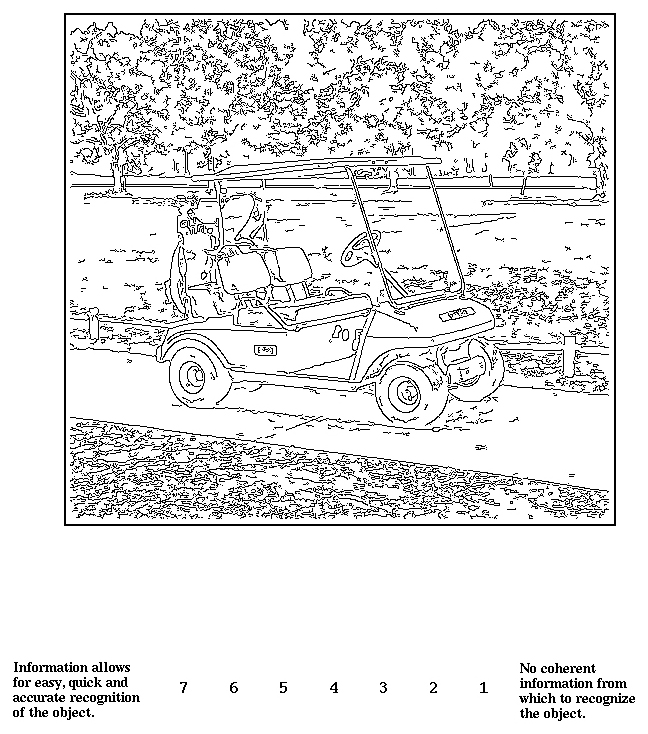
\includegraphics[width=26pc]{gfx/edges-golf.jpg}\caption[\textsc{Item} del cuestionario de \textsc{Heath \etal} \citep{heath97}:\emph{Imagen--pregunta para la evaluaci�n de la calidad de bordes.}]{\textsc{Item} del cuestionario de \textsc{Heath \etal} \citep{heath97} }\label{fig:heath}
\end{SCfigure}

\noindent Finalmente, se pas� a la fase de evaluaci�n mediante cuestionarios. Las im�genes de bordes obtenidas mediante el conjunto reducido de configuraciones para los par�metros de los diferentes algoritmos fueron evaluadas sin l�mite de tiempo por los individuos anteriormente seleccionados. Se les permiti� comparar las distintas im�genes tantas veces como deseasen. Los encuestados valoraron cada imagen de contornos respondiendo a la pregunta:\\[1em]
\begin{tabular}{|B|}
\hline
\emph{Califique la calidad de los bordes para reconocer el objeto central presente en la imagen original}.\vspace{1em}\\
\hline
\end{tabular}\vspace{1em}\\

\noindent La respuesta se encontraba graduada utilizando una \emph{escala de Lickert} entre 1 y 7, donde 1 significaba ``\emph{Los bordes no proporcionan informaci�n coherente que permita reconocer el objeto}'' y 7, ``\emph{Los bordes proporcionan informaci�n que permite un reconocimiento sencillo, r�pido y preciso del objeto}''. En la Fig. \ref{fig:heath} se muestra un \textsc{item} del cuestionario.
\section{Conclusiones}
\lettrine{E}{n} este cap�tulo se han mostrado los dos tipos diferentes de mecanismos de evaluaci�n de resultados, los m�todos \textsc{objetivos} y los m�todos \textsc{subjetivos}. En particular, se ha podido observar que, con car�cter general y debido a las caracter�sticas especiales de las im�genes, los m�todos de evaluaci�n de �stas han de ser \textsc{subjetivos}. Para aplicar estos mecanismos, se ha descrito la m�trica \textsc{MOS}, junto con la extensi�n de la misma propuesta por \person{Durucan \etal}. Tambi�n se ha descrito la metodolog�a de \person{Heath \etal} para la evaluaci�n de las im�genes de bordes.\\
\noindent Los trabajos de \person{Heath \etal} sirven como un punto de inicio contrastado cient�ficamente para la creaci�n de encuestas sobre la calidad subjetiva de im�genes de bordes. Esta metodolog�a, sin embargo, presenta ciertas limitaciones, por ejemplo, no es posible incorporar informaci�n de tipo objetivo, todas las preguntas han de tener el mismo grado de importancia en la respuesta global, todas las preguntas son del mismo tipo (todas tienen un mismo texto de pregunta y se utiliza la misma \emph{escala de Lickert}), por lo que no hay posibilidad de realizar preguntas dicot�micas (S�/No), etc. Gran parte de estas limitaciones se podr�an resolver utilizando el m�todo propuesto por \person{Durucan \etal} utilizando las respuestas obtenidas a partir de encuestas construidas seg�n la metodolog�a propuesta por \person{Heath \etal}.\\
\noindent Tras este cap�tulo se puede afirmar que el mecanismo m�s fiable para evaluar la calidad de las im�genes de bordes es mediante alg�n mecanismo \textsc{Subjetivo}. La evaluaci�n \textsc{Subjetiva} requiere conocer la opini�n de diferentes usuarios, obtenido utilizando \textsc{Encuestas} o \textsc{Cuestionarios}. En el Cap�tulo \ref{chap:encuestas} se describir�n sus caracter�sticas, los inconvenientes que presentan, los problemas asociados y las recomendaciones que, con car�cter general, se han de seguir en su dise�o para construir buenos \textsc{Cuestionarios}.
\myChapter{Encuestas}\label{chap:encuestas}
\minitoc\mtcskip
\vfill
\lettrine{H}{abitualmente}, la captaci�n y la evaluaci�n de la opini�n de usuarios se realiza utilizando cuestionarios o encuestas. Estas encuestas trasladan la opini�n de la poblaci�n (o al menos de una parte representativa de la misma) mediante las preguntas de dichos cuestionarios. La literatura cient��fica actual sobre cuestionarios se centra principalmente en cuestionarios de tipo ``ling\"{u}��stico'' en �reas de investigaci�n econ�micas o sociales. Por tanto, el dise�o de cuestionarios adecuados para la evaluaci�n de la calidad del procesamiento de im�genes es un gran reto.\\
\noindent En este cap��tulo se presentar�n algunas ideas de c�mo deben dise�arse los cuestionarios y qu� problemas y limitaciones presentan los mismos. Se describir�n diferentes tipos de sesgo que pueden afectar a las encuestas y se mostrar�n preguntas de ejemplo que presentan algunos de los problemas y sesgos descritos. Finalmente, se expondr�n brevemente varios m�todos de an�lisis de cuestionarios para estudiar la validez y la fiabilidad de los cuestionarios.
\vfill
\section{Encuestas de opini�n mediante cuestionarios}\label{sec:encuestas}
\lettrine{D}{iversos} autores han estudiado las etapas en las que se divide un \emph{estudio de investigaci�n}. Entendiendo dicho \emph{estudio de investigaci�n} como un proceso cient��fico mediante el cual se pretende evaluar la veracidad de unas hip�tesis de trabajo a partir de datos obtenidos de una poblaci�n (sea humana o no). \person{Burgess} \citep{burgess01} propone una lista concisa de 7 pasos:
\begin{enumerate}
\item Definir el prop�sito de la investigaci�n; fijar los objetivos de la misma.
\item Identificar la poblaci�n y la muestra poblacional.
\item Determinar c�mo recabar las respuestas.
\item Dise�ar el cuestionario.
\item Realizar una encuesta piloto en una muestra poblacional controlada.
\item Realizar la encuesta global con el cuestionario final.
\item Analizar los datos de la encuesta global.
\end{enumerate}

\noindent La lista anterior es bastante general y cada etapa puede presentar una complejidad elevada, as�� pues, \person{Oppenheim} \citep{oppenheim00} ampl��a y profundiza la lista, extendiendo la misma a 12 etapas o pasos:

\begin{enumerate}
\item Decidir cu�les son los \emph{prop�sitos} del estudio, tanto generales como espec��ficos. Traducir estos \emph{prop�sitos} en \emph{objetivos funcionales} (esto es, el conjunto de hip�tesis que se desean investigar). Mediante estos \emph{objetivos funcionales} se construir� la definici�n de las \emph{variables} que se desean medir mediante las \emph{preguntas}.
\item Realizar una revisi�n bibliogr�fica de la literatura cient��fica.
\item Conceptualizar de manera preliminar el estudio: Entrevistas exploratorias.
\item Decidir el dise�o del estudio y determinar su viabilidad.
\item Decidir qu� hip�tesis se investigar�n: crear un listado de \emph{objetivos funcionales} y de variables que se desean ``medir''.
\item Determinar la muestra poblacional que ser� necesaria para obtener un muestreo v�lido: Representatividad, grupos de control, grupo de seguimiento, etc.
\item Seleccionar los sujetos de la muestra poblacional que participar�n el estudio de manera efectiva.
\item Realizar el trabajo de campo: proceso de recolecci�n de datos mediante entrevistas o cuestionarios.
\item Procesar los datos: codificar los resultados y preparar los datos para su posterior an�lisis.
\item Analizar los resultados mediante un estudio estad��stico.
\item Conjuntar todos los resultados y comprobar que las hip�tesis se cumplen con los datos obtenidos.
\item Escribir el informe final.
\end{enumerate}

\noindent Ambas listas est�n dise�adas teniendo en mente la finalidad de la obtenci�n de resultados v�lidos, por lo que es de vital importancia definir correctamente los objetivos que se persiguen con el estudio de investigaci�n. Estos objetivos son los que determinar�n las dem�s etapas, ya que mediante la definici�n de los mismos podremos determinar la poblaci�n destino y qu� muestra poblacional debemos tomar de dicha poblaci�n.\\
\noindent Por ejemplo, si el objetivo deseado es estudiar el grado de aceptaci�n de un nuevo biber�n en Andaluc��a para una posible comercializaci�n del mismo, la poblaci�n destino ser�n los beb�s menores de 1 a�o. De esta manera, teniendo en cuenta la concreci�n espacial y los l��mites temporales, se reduce el universo completo de seres humanos del mundo: el estudio se centra en los beb�s menores de un a�o que viven en Andaluc��a. Tambi�n se puede especificar la muestra poblacional que se tomar� para obtener resultados estad��sticamente �tiles. Para ello, se determina qu� individuos se escoger�n de entre la poblaci�n inicial partiendo desde el objetivo inicial: calculando el grado de inter�s de cada individuo conforme se vayan tomando de la poblaci�n, o bien, escogi�ndolos previamente.\\
\noindent En general, como se puede observar en ambas listas propuestas, el desarrollo de una encuesta y la captaci�n efectiva de las respuestas de los entrevistados son s�lo dos de las etapas que componen el \emph{estudio de investigaci�n}.
\section{?`Qu� es un cuestionario?}
\lettrine{L}{os} cuestionarios son los mecanismos m�s habituales para recoger informaci�n de las encuestas de opini�n. El dise�o de los cuestionarios es una de las etapas m�s importantes dentro de un estudio de investigaci�n mediante encuestas de opini�n. Un buen dise�o del cuestionario, seleccionando bien las preguntas y las respuestas posibles, permitir� obtener respuestas de los entrevistados con las que proporcionar una conclusi�n que describa la opini�n de dichos entrevistados.
\subsection{Definici�n de qu� es un cuestionario}
La \definicion{\textsc{RAE}}{Real Academia Espa�ola de la Lengua} presenta en la $22^a$ Edici�n del Diccionario de la Lengua Espa\-�ola \citep{drae02} una entrada para la palabra \emph{cuestionario} que en su $2^a$ acepci�n se define como:\\[1em]
\begin{tabular}{|A|}
\hline
\textsc{Cuestionario}: {\small sust. m. (lat. \emph{quaestionarius})}\\
\vspace{-1em}\hspace{1em}2. \emph{``Lista de preguntas que se proponen con cualquier fin''}.\vspace{1em}\\
\hline
\end{tabular}\\[1em]
\noindent Esta definici�n, aunque muy formal y acad�mica, es muy vaga, y si no se contextualiza, es poco �til para su aplicaci�n en un �mbito cient��fico, por lo que, un cuestionario se podr��a definir como:\\[1em]
\begin{tabular}{|A|}
\hline
\textsc{Cuestionario}: \emph{``Conjunto de listas de preguntas que se utilizan para obtener informaci�n sobre lo que la gente opina, piensa o siente relativo a un servicio, producto o cuesti�n en particular, con un prop�sito espec��fico previamente fijado por el investigador que lo ha dise�ado''.}\vspace{1em}\\
\hline
\end{tabular}\\[1em]
\noindent Estas listas de preguntas pueden estar impresas o no, se pueden rellenar directamente por parte de los entrevistados o mediante entrevistadores que realicen las preguntas y cataloguen las respuestas, pueden \graffito{Los cuestionarios son herramientas muy flexibles y vers�tiles para obtener la opini�n de una poblaci�n.} realizarse de manera individual o grupal, etc. Como se puede observar, la taxonom��a de cuestionarios que se ha presentado es extremadamente amplia, lo cual, aunque parezca un contrasentido, puede llegar a ser tanto una ventaja como una complicaci�n.\\
\noindent La ventaja se presenta porque se tiene disponible una herramienta tremendamente flexible, que va a permitir el acceso a muchas personas desde diferentes frentes de exploraci�n y la obtenci�n de muchos datos, que pueden ser:
\begin{description}
\item[Datos directos] Respuestas expl��citas de los entrevistados. Ej: \emph{?`Qu� edad tiene Vd.?}
\item[Datos indirectos] Deducciones obtenidas a partir de las respuestas de los entrevistados, pero no obtenidas directamente de una pregunta. Ej: Podemos obtener el rango de riqueza (rico, medio, pobre) a partir de los ingresos anuales, de los gastos habituales, etc.
\item[Relaciones ocultas] Deducciones obtenidas al cruzar los datos de una poblaci�n con diversas variables y de las que previamente no se conoc��a su interrelaci�n. Ej: Deducir que en una poblaci�n de ancianos en un lugar espec��fico el principal problema deja de ser el de \emph{subir escaleras} conforme los ancianos comienzan a interaccionar diariamente con otros ancianos fuera de su hogar.
\end{description}
\noindent La complicaci�n en el dise�o de las encuestas viene por la gran versatilidad disponible al existir tantos formatos diferentes de preguntas y tantas modalidades distintas para la captaci�n de las respuestas. Adem�s, \apriori, no es posible saber si un mecanismo de captaci�n de respuestas es mejor que otro para una determinada poblaci�n, si una pregunta est� bien formulada para obtener un resultado v�lido, etc.
\clearpage
\subsection{Caracter�sticas buscadas con los cuestionarios}
El principal cometido que se persigue con un cuestionario es:\\[1em]
\begin{tabular}{|>{\color{black}\columncolor{colorCorporativoSuave}}p{0.89\textwidth}|}
\hline
\emph{Conseguir respuestas de los entrevistados basadas en \textsc{Opiniones Propias} que proporcionen una \textsc{Informaci�n Generalizable} mediante la cual contrastar la veracidad de unas hip�tesis}.\vspace{1em}\\
\hline
\end{tabular}\\[1em]
\noindent De la aseveraci�n anterior hay que resaltar unos conceptos:
\begin{itemize}
\item Se desean obtener respuestas que expresen \textsc{Opiniones Propias}, por lo que la respuesta de cada entrevistado debe provenir exclusivamente de su propio conocimiento y capacidad de decisi�n, y en ning�n caso debe estar influenciada por elementos externos, es decir, la respuesta no debe estar \textsc{sesgada}.
\item Las respuestas de los entrevistados deben proporcionar \textsc{Informaci�n Generalizable}. La cual involucra todas aquellas evidencias e indicios que son comunes a un colectivo, es decir, que no son exclusivas de un individuo, por lo que de ellas se podr�n deducir opiniones v�lidas para una poblaci�n.
\end{itemize}

\noindent Para que las opiniones que se obtengan de los individuos sean \emph{\textsc{universales}}, la muestra de individuos a los que se les realice la entrevista ha de ser seleccionada minuciosamente en una fase previa al dise�o de las preguntas. Esta selecci�n deber��a garantizar que la muestra poblacional escogida representa completamente a la poblaci�n universo.
\section{Mecanismos de recolecci�n de las respuestas}
\lettrine{U}{n} aspecto muy importante, que determina en gran modo el dise�o de los cuestionarios, es definir c�mo se obtendr�n las respuestas de los encuestados. Existen 2 tipos principales de mecanismos de recolecci�n de respuestas:
\begin{aenumerate}
\item Entrevistas estructuradas.
\item Cuestionarios auto--administrados.
\end{aenumerate}

\noindent A continuaci�n, se describen los dos mecanismos de recolecci�n de datos, tras lo que se expondr�n brevemente los tipos de preguntas m�s habituales.
\subsection{Entrevistas estructuradas}
La recolecci�n de respuestas mediante ``entrevistas estructuradas'', involucra a un entrevistador, que gu��a la entrevista seg�n las respuestas del entrevistado. Estas entrevistas se realizan generalmente cara a cara o mediante llamada telef�nica. El hecho de que el entrevistador realice de manera oral las preguntas, con una \emph{realimentaci�n} inmediata por parte de los entrevistados, hace que las frases se propongan de manera diferente a como se har��a si estas preguntas se hicieran por escrito. En este tipo de cuestionarios, adem�s de incluir frases para los entrevistadores, estos deben ser instruidos para que sepan responder a las dudas que les surjan a los entrevistados, as�� como para que sean capaces de llevar una encuesta din�mica y �gil. Usualmente, estas encuestas son de corta duraci�n (no suelen superar los 10 minutos en el peor de los casos), y est�n recomendadas para la obtenci�n de estados de opini�n puntuales (por ejemplo, en elecciones y votaciones).\\[1em]
\noindent Sus grandes ventajas son: su inmediatez y su alta tasa de respuestas (salvo para encuestas que involucren aspectos de tipo sensible, en los que responder directamente a una persona pueda provocar rechazo). En cuanto a sus desventajas, el coste de este tipo de encuestas es elevado, lo que limita bastante el n�mero de encuestados. Adem�s, las respuestas tienen una alta probabilidad de ser ``pol��ticamente correctas'' al hacerse delante de una persona. Por �ltimo, su principal problema es que s�lo pueden ser de tipo general, es decir, que no involucren procesos mentales excesivamente complejos, ya que en dichos casos, la mayor��a de los encuestados abandonan.
\subsection{Cuestionarios auto--administrados}
El otro gran grupo de cuestionarios se denomina, de manera general, ``cuestionarios auto--administrados''. Al contrario que los anteriores no involucran la presencia activa de un entrevistador durante el proceso de recolecci�n de las respuestas. Por tanto, es necesario a�adir unas instrucciones precisas para los entrevistados, y que las preguntas se dise�en de forma que no surjan dudas. Se suele admitir que estos cuestionarios no se responden en una �nica sesi�n, as�� que deben dise�arse para poder dejarlos y continuar en otro momento. Debido a esto, los ``cuestionarios auto--administrados'' suelen ser m�s largos e incluir m�s preguntas que los que se realizan mediante ``entrevistas estructuradas''. Este mecanismo est� espec��ficamente indicado para poblaciones muy dispersas y dif��cilmente accesibles mediante entrevistas directas.\\[1em]
\noindent Presentan ciertas ventajas: son mucho m�s baratos que las ``entrevistas estructuradas'', permiten recolectar datos de procesos mentalmente m�s complejos (ya que el encuestado tiene m�s tiempo para responder) y permiten hacer preguntas de aspectos m�s sensibles. Sin embargo, entre desventajas destacan su bajo nivel de respuesta, su lentitud y, sobre todo, el poco control que se tiene sobre las respuestas: el entrevistador ``tiene que fiarse'' de que las respuestas est�n realmente meditadas (que no han sido respondidas sin reflexionar), y de que han sido proporcionadas por el propio entrevistado (no por otra persona).
\clearpage
\subsection{Tipos de preguntas}
La tipolog��a de preguntas posibles en un cuestionario es muy amplia, a continuaci�n se muestra un breve resumen de las principales categor��as:
\begin{aenumerate}
\item \person{\textsc{Seg�n la elecci�n de las respuestas}}
    \begin{description}
        \item[Abiertas] Todas las respuestas son posibles, de manera que no existe una lista de respuestas entre las que escoger.
        \item[Cerradas] S�lo se admiten como posibles respuestas las existentes dentro de una lista de opciones previamente dise�ada por el encuestador.
        \item[Semicerradas] Se le proponen al encuestado una lista de posibles respuestas (habitualmente, las consideradas m�s comunes) y se le proporciona la opci�n de a�adir otra respuesta de manera libre.
    \end{description}
\item \person{\textsc{Seg�n el tipo de las respuestas}}
    \begin{description}
        \item[Dicot�micas] Las respuestas son del tipo \mbox{verdadero/falso}, \mbox{s��/no} u otras opciones similares.
        \item[Categorizadas o de escala ordinal] Las respuestas suelen ser adjetivos o adverbios, que describen alg�n tipo de graduaci�n subjetiva, con los que los encuestados responden a las preguntas.
        \item[Valoraci�n o de escala num�rica] Las respuestas son valores num�ricos que tienen asociado un orden que permite a los encuestados proporcionar su grado de aceptaci�n o rechazo respecto a lo planteado en la pregunta. Tambi�n pueden indicar el orden relativo entre las distintas opciones planteadas.
    \end{description}
\item \person{\textsc{Seg�n la captura de los datos deseados}}
    \begin{description}
        \item[Directas] Si se pregunta directamente al encuestado por la variable que se desea medir.
        \item[Indirectas] Si se pregunta al encuestado por otra cuesti�n, que permite determinar la variable deseada.
    \end{description}
\item \person{\textsc{Seg�n el n�mero de respuestas por pregunta}}
    \begin{description}
        \item[Respuesta �nica] S�lo se admite una respuesta por pregunta.
        \item[Respuesta m�ltiple] Es admisible proporcionar varias respuestas para una misma pregunta. Dentro de este tipo de preguntas se tienen dos divisiones:
        \begin{itemize}
            \item \emph{Respuestas m�ltiples sin repetici�n}: Se admiten varias respuestas por pregunta pero no es posible repetir varias veces la misma respuesta.
            \item \emph{Respuestas m�ltiples con repetici�n}: Se admiten varias respuestas para una misma pregunta y es posible seleccionar la misma respuesta varias veces.
        \end{itemize}
    \end{description}
\end{aenumerate}
\section{Limitaciones de los cuestionarios}
\lettrine{A}{ntes} de estudiar m�s a fondo los cuestionarios, conviene saber qu� se puede obtener utilizando los estudios basados en encuestas. Estos estudios pueden servir tanto como instrumentos de recogida de datos, como mecanismos para el an�lisis de variables indirectas. Esta gran versatilidad permite su aplicaci�n en muchas tem�ticas diferentes. Por tanto, para todos aquellos que se acercan por primera vez a las encuestas existe una tendencia generalizada a pensar que �stas ``\emph{son comodines que sirven para todo}'' \citep{alviramartin04}. Sin embargo, las encuestas muestran limitaciones y condicionantes que hacen que �stas no sean v�lidas en todos los casos.\\
\noindent Por ejemplo, las encuestas no son apropiadas para investigar las razones, motivos o causas subjetivas de comportamientos o fen�menos poco conocidos, en poblaciones peque�as o poco frecuentes y/o dif��ciles de acceder. La encuesta es un m�todo dirigido a la descripci�n y a la constataci�n de hip�tesis, m�s que al descubrimiento o a la elaboraci�n de hip�tesis o teor��as. A continuaci�n, se mostrar�n algunas de las cr��ticas m�s habituales que se hacen a las encuestas.
\begin{description}
\item[Falta de objetividad] Los resultados de las encuestas dependen del contexto del significado e interpretaci�n de las preguntas por parte de los entrevistados. Adem�s, la perspectiva te�rica que se haya escogido influye en la informaci�n recogida (\emph{s�lo se puede encontrar lo que se busca}).
\item[Influencia en las respuestas] Las propias preguntas realizadas en las encuestas pueden crear opiniones \emph{ex novo} en individuos que no han reflexionado nunca sobre un tema.
\item[Atomismo] La informaci�n que surge de la encuesta, en muchos casos, es una mera agregaci�n de respuestas individuales que no tienen en cuenta interacciones sociales, relaciones, ni otros aspectos relativos a la estructura social que no se hayan tenido en cuenta en el modelo conceptual con el que se ha dise�ado el cuestionario.
\item[Captura est�tica de la realidad] Los resultados de las encuestas muestran, en el mejor de los casos, una ``fotograf��a'' est�tica de las opiniones en un momento puntual. Esto obligar��a a realizar estudios en distintos instantes temporales, con la consiguiente dificultad para integrar todas las opiniones.
\item[Limitaci�n del �mbito de aplicaci�n] Las encuestas no est�n previstas para �mbitos de estudio en los que las medidas no se puedan obtener mediante preguntas subjetivas. Por ejemplo, en los �mbitos de ciencias naturales es absurdo realizar los estudios utilizando encuestas, puesto que en la mayor��a de los casos, no se puede preguntar a los sujetos (no son humanos, pueden ser animales, plantas, etc.). Adem�s, en estos �mbitos las medidas objetivas son m�s precisas y se pueden obtener directamente.
\item[Costes elevados] La realizaci�n de un estudio de investigaci�n mediante cuestionarios es caro, tanto en tiempo como en costes econ�micos y medios materiales y humanos.
\end{description}

\noindent Como resumen, se puede afirmar que las encuestas son instrumentos estructurados de captura de informaci�n, que podr��an influir en la informaci�n recogida. Los cuestionarios son �tiles, ante todo, para describir y contrastar hip�tesis o modelos. Por el contrario, no son recomendables para construir teor��as o para deducir hip�tesis nuevas.
\section{Fuentes de error en los cuestionarios}
\lettrine{L}{a} validez de los resultados que se obtengan de un cuestionario depender� de qu� se ha preguntado, c�mo se ha preguntado, a qui�n se le ha preguntado, qu� opciones se han ofrecido para responder, en qu� contexto se ha realizado la pregunta y otros aspectos relacionados con la encuesta y con su administraci�n. A veces, los resultados obtenidos a partir de una encuesta var��an con respecto a la opini�n real de la poblaci�n, obtenida mediante otras encuestas o bien utilizando otros cuestionarios que han sido validados previamente. Dicha variaci�n es debida a la presencia de errores, que pueden ser \emph{sistem�ticos} o \emph{aleatorios}. Los errores \emph{aleatorios} no tienen gran incidencia en el conjunto de la encuesta, puesto que ni sobreestiman ni subestiman los valores promedio, y si la muestra poblacional es suficientemente grande, pueden mitigarse f�cilmente. Sin embargo, los errores \emph{sistem�ticos} pueden llegar a producir un falso aumento o disminuci�n del valor promedio, produciendo un \definicion[-3em]{sesgo}{Error que aparece en los resultados que puede conducir a conclusiones que son sistem�ticamente diferentes de la verdad o incorrectas.} en los resultados. Estos sesgos pueden tener su origen en el dise�ador de la encuesta, el encuestador o los entrevistados y, a su vez, pueden ser intencionados o no. La mayor��a de errores provienen del dise�o del cuestionario y de las preguntas, dentro de las que las principales fuentes de error son \citep{ceadancona04}:\\
\person{\textsc{Errores de especificaci�n conceptual}} El modelo subyacente sobre el que se construye la encuesta est� mal construido.
\begin{aenumerate}
\item \emph{Problemas de connotaci�n}: Confusi�n de significados porque el modelo est� asociado a m�s de un significado o porque hay varios modelos diferentes que pueden responder al mismo significado y los investigadores no han hecho expl��cito lo que pretenden.
\item \emph{Problemas de denotaci�n}: Modelos d�bilmente definidos y ``vagos'' en cuanto a su precisi�n, en los que no est�n claramente especificados los objetos, entidades o referentes a los que se aplica.
\item \emph{Problemas terminol�gicos}: Fallos de elecci�n de etiquetas lin\-g\"{u}��s\-ti\-cas o conceptuales para definir el modelo que inducen a ca\-rac\-te\-r��s\-ti\-cas o referentes err�neos.
\end{aenumerate}


\noindent \person{\textsc{Errores debidos a la formulaci�n de las preguntas}} Las preguntas o las opciones de respuesta provocan que los encuestados escojan una opci�n distinta a la opini�n real que tienen sobre los objetivos de investigaci�n asociados a cada pregunta.

\begin{aenumerate}
\item \textsc{Sesgo de especificaci�n}: \noindent No existe una correspondencia entre la pregunta y los objetivos de la investigaci�n: se est� haciendo una pregunta que no mide realmente lo que se hab��a planteado en los objetivos del cuestionario.
\item \textsc{Sesgo de medici�n}: \noindent La pregunta est� bien planteada y est� acorde con los objetivos del cuestionario, pero la respuesta que proporcionan los encuestados no coincide con su opini�n real.
\begin{enumerate}
\item \emph{Sesgo de interpretaci�n de t�rminos}: \noindent Se produce al introducir palabras ambiguas o con diferentes connotaciones, que pueden ser interpretados por los encuestados de diferente manera a como fueron ideadas por el dise�ador de la encuesta.
\item \emph{Sesgo de redacci�n}: \noindent La redacci�n de la pregunta hace que el entrevistado tenga cierta tendencia a escoger una determinada respuesta.
\item \emph{Sesgos debidos al orden de las respuestas}, (\emph{Sesgo de pri\-ma\-c�a}, \emph{Sesgo de recencia}): \noindent Dependiendo del tipo de encuesta, el orden en el que se ofrecen las respuestas a los entrevistados puede hacer que se seleccione preferentemente alguna de ellas. En las encuestas en las que los entrevistados no pueden visualizar las opciones, existe una tendencia a seleccionar la primera alternativa que se mencione (\emph{efecto de primac��a}) o la �ltima (\emph{efecto de recencia}), con independencia del contenido de la respuesta en s��.
\item \emph{Sesgo de contexto}: \noindent Los encuestados suelen interpretar los cuestionarios como preguntas enlazadas una tras otra y construyen relaciones internas entre las diferentes preguntas, de tal forma, que las respuestas de una pregunta suelen estar influenciadas en las preguntas anteriores y posteriores, es decir, en el \emph{contexto de la pregunta}.
\item \emph{Sesgo de deseabilidad social}: \noindent En los cuestionarios que se pregunta por aspectos sensibles que pueden inhibir al encuestado a dar una respuesta veraz, en muchos casos, lo que se obtiene no es la opini�n real que tiene el entrevistado sino respuestas ``pol��ticamente correctas'' o socialmente deseables. Tambi�n aparece este tipo de sesgo cuando elige una respuesta que �l cree que es la que se espera que d�, es decir, cuando el encuestado se quiere ajustar a las expectativas o demandas del investigador.
\item \emph{Sesgo de aquiescencia}: \noindent Este sesgo se produce cuando el encuestado elige la respuesta afirmativa o que el entrevistado cree que supone un mayor consenso.
\item \emph{Sesgo de repetici�n de respuestas}: \noindent Cuando hay muchas preguntas seguidas que tienen las mismas opciones de respuesta, los entrevistados pueden llegar a mostrar una tendencia a repetir las mismas respuestas pregunta tras pregunta.
\item \emph{Sesgo de aversi�n de extremos}: \noindent En las preguntas con respuestas categorizadas, los encuestados tienden a evitar los extremos, en particular si estos son absolutos (no suelen escoger opciones como ``siempre'' o ``nunca'', sino ``casi siempre'' o ``casi nunca'').
\end{enumerate}
\end{aenumerate}

\noindent Estos sesgos han sido ampliamente estudiados \citep{ceadancona04,alviramartin04,estadisticaURL} y existen muchos trabajos para evitar en la medida de lo posible la influencia de estas fuentes de error.\\
\noindent Adem�s de los anteriores sesgos, que aparecen debidos al dise�o del cuestionario y de las preguntas, existen otras fuentes de error adicionales, introducidas por otras causas diferentes a las anteriormente citadas, entre las que cabe destacar:
\begin{description}
\item[Errores poblacionales] Est�n debido a una mala selecci�n de la muestra de la poblaci�n sobre la cual se realizar� el estudio. Suelen llamarse \emph{Sesgo por selecci�n} o \emph{Sesgo poblacional}.
\item[Errores por no respuesta] En los casos en los que no se responda el cuestionario completo, o a una pregunta determinada de dicho cuestionario, hay que determinar el porqu�. Puede ser por desconocimiento de la tem�tica que se pregunta, por negarse a compartir la informaci�n de dicha cuesti�n, por omisi�n involuntaria, etc. Todas aquellas preguntas que no son respondidas por los encuestados, pueden alterar el resultado promedio completo, o bien, dar una excesiva importancia a las respuestas proporcionadas por otros encuestados, desplazando el resultado hacia la opini�n personal de uno de esos encuestados y no hacia la opini�n global, a lo que se le llama \emph{Sesgo por no respuesta}.
\item[Errores de finalidad] Cuando el encuestado conoce (o cree conocer) la finalidad u objetivo asociado una pregunta y adapta su respuesta a dicha finalidad u objetivo. Se denomina \emph{Sesgo por finalidad}.
\end{description}

\noindent En la secci�n \ref{sec:poblacion}, se profundizar� sobre el \emph{Sesgo por selecci�n}. El segundo tipo (\emph{Sesgo por no respuesta}) se suele dar en las encuestas de tipo personal o en las que hay que dar una opini�n de tipo subjetivo; en estas situaciones, es posible que los entrevistados no se atrevan o no sean capaces de responder a algunas preguntas. El \emph{Sesgo de deseabilidad social} aparecer��a en los casos en que estas preguntas se respondan, pero con respuestas ``pol��ticamente correctas'', diferentes de la opini�n real de los entrevistados. Otra opci�n posible es que se produzcan respuestas al azar por desconocimiento del tema, aunque no ser��a demasiado grave, puesto que no generar��a un error sistem�tico, sino aleatorio, que se podr��a mitigar con una muestra poblacional suficientemente amplia. El tratamiento de la ``no repuesta'' en cuestionarios tiene una vital importancia, ya que puede alterar completamente los resultados promedio, por un lado, proporcionando excesiva importancia a aquellos cuestionarios que s�� han sido respondidos, y por otra parte, porque se ignora el motivo por el cual no se han contestado estos cuestionarios o preguntas. Para evitar, o al menos, limitar  estos efectos, se sugiere introducir en los cuestionarios pilotos, previos al dise�o del cuestionario final, una opci�n de ``No Sabe'' y otra de ``No contesta'' pudiendo indicar el motivo. Estas opciones de respuestas \emph{abiertas} permiten a los investigadores contar con m�s elementos de juicio para un mejor dise�o de las preguntas. Existen muchos trabajos cient��ficos \citep{argimonpallas05,alviramartin04,ceadancona04,estadisticaURL} que se pueden consultar para ampliar informaci�n sobre estos tipos de sesgos y conocer, con mayor detalle, los mecanismos habituales que se pueden utilizar para minimizar el efecto de los mismos.\\
\noindent Finalmente, el \emph{Sesgo por finalidad} es una aportaci�n que realiza el autor de esta Tesis en vista de los resultados obtenidos en el �mbito de las encuestas en las ingenier��as, aunque es f�cilmente exportable a pr�cticamente todos los campos del saber. Este tipo de sesgo se describir� con mayor concreci�n en el Cap�tulo \ref{chap:recCuestCalidadBordes}.

\section{Elecci�n de la muestra poblacional}
\lettrine{U}{na} de las fases m�s importantes en el desarrollo de una encuesta es la elecci�n de un grupo de individuos v�lido y representativo de la poblaci�n sobre la que se obtendr�n las conclusiones. Esta fase puede ser tan simple como un muestreo aleatorio dentro de un grupo poblacional amplio, si se considera que todos los individuos de dicha poblaci�n proporcionan informaci�n con una validez similar, y que no se presentan influencias importantes en sus respuestas. Sin embargo, para encuestas de opini�n en las que las respuestas de los individuos pueden estar muy influenciadas por su estatus, condici�n social, situaci�n geogr�fica, etc., la elecci�n de los individuos para lograr una muestra poblacional no sesgada puede llegar a significar un escollo considerable.\\
\noindent Hay ciertas cuestiones que hay que determinar a la hora de escoger una muestra poblacional \citep{estadisticaURL}:
\begin{itemize}
\item El m�todo de selecci�n de los individuos de la poblaci�n (tipo de muestreo).
\item El tama�o de la muestra poblacional.
\item El grado de fiabilidad de las conclusiones en funci�n de la muestra poblacional escogida (probabilidad del error).
\end{itemize}
\subsection{Selecci�n de individuos}\label{sec:poblacion}
Una selecci�n incorrecta de la muestra poblacional puede provocar errores posteriores a la hora de estimar las correspondientes opiniones de la poblaci�n. Por ejemplo, si la muestra perteneciese a un nicho poblacional poco representativo del total de la poblaci�n, las respuestas y las conclusiones obtenidas no ser��an v�lidas, ya que habr��an sufrido \emph{Sesgo por selecci�n}. Seg�n \person{Lagares} y \person{Puerto} \citep{estadisticaURL}, de manera generalizada, para evitar este sesgo se debe realizar una criba previa en la que se indica cu�ntos individuos se van a tomar, por ejemplo, de cada determinada edad, en cada zona, y con qu� caracter��sticas en particular. Para realizar esta criba \apriori se aplican unas t�cnicas, denominadas ``de muestreo'', que se exponen a continuaci�n:
\begin{aenumerate}
 \item Muestreo al azar (con y sin reemplazamiento).
 \item Muestreo estratificado.
 \item Muestreo por conglomerados o por racimos.
 \item Muestreo sistem�tico.
\end{aenumerate}

\noindent Tambi�n se pueden dar mezclas entre ellas, como por ejemplo, en el caso del muestreo estratificado por conglomerados, en el que la poblaci�n se subdivide en distintos conglomerados lo m�s homog�neos entre s�� que a su vez se tratan de manera estratificada (seg�n diferentes conceptos geogr�ficos, sociales, etc.).\\
\noindent Sin embargo, no siempre se puede aplicar una criba previa a la encuesta, ya que a veces se desconoce la clasificaci�n de cada individuo dentro de la muestra poblacional, por lo que para estos casos, lo que se realiza es un descarte \emph{a posteriori} de aquellas respuestas que se desv��en en exceso del comportamiento medio, trat�ndolas como valores an�malos o extremos.
\subsubsection{Tama�o de la muestra}
Aunque se sabe que cuanto mayor sea el tama�o de la muestra poblacional, menor ser� el error inferido, factores como el coste econ�mico, la disponibilidad de tiempo, etc., suelen poner limitaciones a la hora de fijar el valor de este par�metro. Por ello, previamente se debe conocer el tama�o m��nimo que deber��a tener la muestra poblacional para que las conclusiones que se extraigan de las respuestas de los entrevistados sean representativas de la opini�n de toda la poblaci�n. Existen f�rmulas que determinan estad��sticamente este valor, en funci�n del error m��nimo admisible, de si es conocida o no la varianza poblacional, de si se conoce el n�mero de individuos de toda la poblaci�n, etc. En general, el tama�o de la muestra viene determinado por el nivel de confianza que se pueda obtener de las conclusiones utilizando un determinado tama�o de muestra poblacional. De tal forma que cuanta mayor precisi�n se requiera para las conclusiones, mayor deber� ser el tama�o de la muestra exigida.
\subsubsection{Grado de fiabilidad de los resultados}
Como se ha visto en apartados anteriores, todas las decisiones que se toman con respecto al dise�o de una encuesta se realizan teniendo en cuenta las conclusiones que se pretendan obtener. En particular, si se desean unas conclusiones muy precisas, ser� necesaria una muestra amplia, en la que los individuos se hayan seleccionado con una precisi�n elevada, rechazando aquellos que pudieran falsear los resultados generales. En cambio, si simplemente son admisibles unos resultados que muestren \emph{grosso modo} los aspectos principales de una determinada poblaci�n, bastar� con una muestra de tama�o reducido y un proceso de selecci�n de individuos no excesivamente exigente.\\
\noindent Sin embargo, puede que en algunas ocasiones no exista la posibilidad de elegir a los individuos que formar�n parte de la muestra. En estos casos, es interesante calcular el grado de fiabilidad de los resultados obtenidos en funci�n del tama�o de la selecci�n de la muestra poblacional.\\
\noindent Para cada una de las variables cuyo valor se intenta obtener mediante la encuesta, su grado de fiabilidad se puede determinar como un valor �nico o como un intervalo de confianza. En ambos casos, se realiza una estimaci�n de la distribuci�n estad��stica que modela cada medida observada, y en funci�n de dicha distribuci�n, se determina el valor (o el intervalo de valores) que delimita el l��mite que permitir��a identificar un valor concreto de esa medida dentro de un rango v�lido o aceptable para dicha variable. Las distribuciones estad��sticas m�s utilizadas para este prop�sito son la distribuci�n Normal o Gaussiana, la $\chi^2$, la uniforme, la ``t'' de Student, la ``F'' de Snedecor, etc. De entre ellas, se escoger� la que mejor se ajuste a los valores de cada variable.
\section{Dise�o de un cuestionario}\label{sec:diseno-cuestionario}
\lettrine{C}{omo} se ha mostrado en la Secci�n \ref{sec:encuestas}, el dise�o del cuestionario es s�lo uno de los pasos del proceso de estudio de investigaci�n mediante cuestionarios. Sin embargo, aunque todos los pasos citados con anterioridad son imprescindibles para obtener datos fiables y �tiles, el desarrollo del cuestionario es la etapa del proceso que m�s esfuerzo requiere y en la que mayor cantidad de decisiones se han de tomar. As�� pues, suponiendo que el resto de pasos necesarios para la realizaci�n de una encuesta de opini�n se han realizado previamente, el dise�o de un cuestionario se puede dividir en tres apartados:
\begin{enumerate}
\item Determinar qu� variable se controla con cada pregunta que se vaya a realizar.
\item Seleccionar la tipolog��a de cada una de las preguntas y especificar su redacci�n.
\item Dise�ar la secuencia de preguntas y la distribuci�n gr�fica general del cuestionario.
\end{enumerate}
\subsection{Dificultades para construir buenas preguntas}
Dentro del �mbito de las encuestas de opini�n hay una obviedad muy clara: \emph{Para obtener buenas respuestas, hay que hacer buenas preguntas a la gente correcta}. A pesar de lo que se muestra en esta afirmaci�n, es \graffito{Las buenas respuestas provienen de buenas preguntas a la gente correcta.} conveniente desmenuzarla para entenderla mejor. Las respuestas ``\emph{buenas}'' son aquellas estad��sticamente relevantes, de las que se pueden obtener deducciones estad��sticas que coincidan con la poblaci�n completa. En cuanto a la gente ``\emph{correcta}'', se entiende que deben ser individuos de una muestra poblacional representativa.\\
\noindent Por tanto, reescribiendo la frase anterior se puede obtener una afirmaci�n menos ``directa'' aunque m�s correcta: \emph{Para obtener respuestas que estad��sticamente proporcionen informaci�n relevante, hay que saber hacer buenas preguntas a los individuos de una muestra poblacional correctamente escogida y suficientemente representativa}.\\
\noindent Lo �nico que ha faltado por concretar es qu� se entiende por \textsc{buenas preguntas}. La respuesta a esta pregunta es bastante complicada, ya que \apriori no es posible determinar si una pregunta es buena o es mala. Sin embargo, existen bastantes trabajos \citep{bradburn04,oppenheim00,hayes99} en los que se recomiendan normas generales para la redacci�n de las preguntas, principalmente para encuestas de tipo social. Ejemplos de estas recomendaciones son:
\begin{itemize}
\item Realizar preguntas para obtener una de las respuestas objeto de estudio, no caer en la tentaci�n de preguntar ``porque es interesante saber algo''. Este tipo de preguntas suelen confundir a los entrevistados, descentr�ndolos del cometido principal.
\item Limitar la longitud de los cuestionarios, ya que los cuestionarios excesivamente largos no se suelen contestar completamente por parte de los entrevistados, o bien, al alargarse el tiempo, no contienen respuestas muy fiables.
\item Comenzar con preguntas sencillas y atrayentes para los entrevistados, a las que no tengan que dedicar excesivo tiempo para pensar la respuesta. Esta estrategia les anima a continuar. Si las preguntas iniciales son demasiado cr��ticas, o implican que los entrevistados les dediquen mucho tiempo para pensar las respuestas, es muy probable que renuncien a continuar con el cuestionario.
\item Utilizar preguntas directas y con un lenguaje simple. Las preguntas enrevesadas, con un lenguaje excesivamente t�cnico, o por el contrario, utilizando jerga, habitualmente no son comprendidas por los entrevistados, y por lo tanto, sus respuestas suelen ser poco fiables.
\end{itemize}

\noindent Las recomendaciones anteriores son de tipo general. Sin embargo, observando determinadas preguntas se pueden deducir otras recomendaciones m�s espec��ficas para la redacci�n de las preguntas en particular. A continuaci�n, se propone un conjunto de preguntas \emph{mal planteadas}, junto con la explicaci�n de porqu� se considera que dichas preguntas no est�n bien formuladas y c�mo rehacerlas para obtener \textsc{buenas preguntas}.

\paragraph{Evitar la Ambig\"{u}edad:} \noindent Estos ejemplos muestran que no se deben dise�ar preguntas que puedan tener m�ltiples interpretaciones o preguntas que fuercen al encuestado a responder de una determinada manera espec�fica.\\[-0.5em]

\begin{tabular}{|p{0.9\textwidth}|}
\hline
\rowcolor{colorCorporativoSuave}\textsc{Ejemplo:}\\
\rowcolor{colorCorporativoSuave}\emph{?`Qu� te gusta m�s, el sabor c��trico o la textura crujiente del helado?}\\
\hline
\rowcolor{colorCorporativoMasSuave}\textsc{Comentario:}\\
\rowcolor{colorCorporativoMasSuave}Se dan demasiadas combinaciones para las respuestas: que al entrevistado le guste el sabor c��trico pero no la textura crujiente, que le gusten ambos, que no le gusten ninguna de las dos, que le guste la textura crujiente pero no el sabor, o incluso que le gusten ambos, pero por separado.\\
\hline
\end{tabular}\graffito{Preguntar por un �nico aspecto en cada pregunta.}\vspace{1em}\\

\begin{tabular}{|p{0.9\textwidth}|}
\hline
\rowcolor{colorCorporativoSuave}\textsc{Ejemplo:}\\
\rowcolor{colorCorporativoSuave}\emph{?`Qu� sistema operativo utilizas en tu PC?}\\
\rowcolor{colorCorporativoSuave}\hspace{1em}\emph{Windows XP o Windows Vista}.\\
\hline
\rowcolor{colorCorporativoMasSuave}\textsc{Comentario:}\\
\rowcolor{colorCorporativoMasSuave}No es una buena pregunta, puesto que se pueden dar otros muchos tipos de sistemas operativos: ninguno, Linux, Solaris, MacOS, otras versiones diferentes de MS Windows, etc.\\
\hline
\end{tabular}\graffito{Cubrir todas las respuestas posibles para cada pregunta.}\vspace{1em}\\

\begin{tabular}{|p{0.9\textwidth}|}
\hline
\rowcolor{colorCorporativoSuave}\textsc{Ejemplo:}\\
\rowcolor{colorCorporativoSuave}\emph{?`Qu� lugares te gustar��a visitar como turista?}\\
\rowcolor{colorCorporativoSuave}\hspace{1em}\emph{Paris, Madrid o Francia.}\\
\hline
\rowcolor{colorCorporativoMasSuave}\textsc{Comentario:}\\
\rowcolor{colorCorporativoMasSuave}Las respuestas no han sido correctamente seleccionadas y pueden presentar dudas a los entrevistados, ya que el que se escoja visitar Francia no es excluyente para escoger Paris.\\
\hline
\end{tabular}\graffito{Selecciona respuestas mutuamente excluyentes entre s��.}\vspace{1em}\\

\noindent Con recomendaciones de este tipo se pretende prevenir la ambig\"{u}edad en las preguntas. Evitando este problema, se trata de obtener de los entrevistados respuestas veraces. La veracidad de las respuestas tiene que venir de dos frentes: los entrevistados deben entender perfectamente lo que se les pregunta y han de tener opini�n propia sobre la cuesti�n.
\paragraph{Preguntas Capciosas y mal planteadas:} \noindent Este contexto abarca tanto las \definicion[-1em]{preguntas capciosas}{Que se dise�an para arrancar al interlocutor una respuesta que favorezca a los prop�sitos de quien las formula, o para que �ste �ltimo gu��e las respuestas del primero en una determinada direcci�n.}, que est�n dise�adas con una intencionalidad predeterminada por parte del encuestador, como las preguntas que, por su redacci�n, provocan una influencia no deseada en la respuesta de los entrevistados, aunque, \apriori no han sido dise�adas con ninguna intencionalidad. Estas recomendaciones pretenden la independencia de las respuestas de los encuestados. �sta proviene principalmente de la necesidad de separar el pensamiento del entrevistado de las ideas preconcebidas del entrevistador: el entrevistado debe responder por s�� mismo, sin ayuda, gu��a o consejo del entrevistador. Es evidente que para que los resultados de la encuesta sean v�lidos, el entrevistador debe evitar expresar cualquier opini�n personal o cualquier resultado general, ya que estos comentarios, sugerencias o datos adicionales suelen condicionar las respuestas.El primer ejemplo introduce informaci�n propia del entrevistador en la pregunta:\\

\begin{tabular}{|p{0.9\textwidth}|}
\hline
\rowcolor{colorCorporativoSuave}\textsc{Ejemplo:}\\
\rowcolor{colorCorporativoSuave}\emph{En lo concerniente a F�rmula 1, sabiendo que Ferrari es la mejor escuder��a, ?`cree Vd. que este a�o conseguir�n revalidar el t��tulo?}\\
\hline
\rowcolor{colorCorporativoMasSuave}\textsc{Comentario:}\\
\rowcolor{colorCorporativoMasSuave}Esta se puede considerar una \textsc{Pregunta Capciosa}: la informaci�n de que Ferrari es la mejor escuder��a es propia del entrevistador y no proporciona informaci�n �til para el entrevistado, por lo que influye (o al menos podr��a influir) en la respuesta del entrevistado. Una pregunta m�s as�ptica y neutral ser��a: \emph{?`Cree Vd. que Ferrari conseguir� revalidar el t��tulo de F�rmula 1 este a�o?}\\
\hline
\end{tabular}\graffito{No introducir opiniones personales del entrevistador en el cuerpo de las preguntas.}\vspace{1em}\\

\noindent En este ejemplo, se a�ade informaci�n general que puede condicionar la respuesta:\\

\begin{tabular}{|p{0.9\textwidth}|}
\hline
\rowcolor{colorCorporativoSuave}\textsc{Ejemplo:}\\
\rowcolor{colorCorporativoSuave}\emph{?`Est� Vd. de acuerdo con la mayor��a de la gente que opina que la econom��a va bien?}\\
\hline
\rowcolor{colorCorporativoMasSuave}\textsc{Comentario:}\\
\rowcolor{colorCorporativoMasSuave}Esta pregunta, \apriori, no puede ser considerada una \textsc{Pregunta Capciosa}, sin embargo, est� mal dise�ada, ya que podr��a inducir un \emph{sesgo de deseabilidad social}. Al introducir informaci�n sobre qu� ha contestado ``la mayor��a de la gente'', se est� proporcionando al entrevistado datos sobre las respuestas que ya se han obtenido. Esto, en cierto modo, obliga al entrevistado a dar una respuesta similar a los dem�s. La pregunta estar��a mejor formulada como \emph{?`Cree Vd. que la econom��a va bien?}\\
\hline
\end{tabular}\graffito{No a�adir datos de opiniones de tipo general que puedan influir en la respuesta.}

\paragraph{Preguntas con exceso de informaci�n:} \noindent Existe otro tipo de condicionamiento de las respuestas, que es mucho m�s sutil, y que en la mayor��a de los casos no se realiza conscientemente por parte del entrevistador. Suele aparecer cuando se incluye informaci�n adicional, datos o descripciones para explicar el entorno en el que se ubica una determinada pregunta. Esta informaci�n puede llegar a modificar o alterar la independencia de los entrevistados, y resulta muy dif��cil, a veces imposible, evitar este efecto.\\

\begin{tabular}{|p{0.9\textwidth}|}
\hline
\rowcolor{colorCorporativoSuave}\textsc{Ejemplo:}\\
\rowcolor{colorCorporativoSuave}\emph{Las tres grandes compa���as de desarrollo de videoconsolas, Sony, Microsoft y Nintendo, han sacado al mercado diferentes consolas de �ltima generaci�n, cada una de �stas con distintos precios (de manera aproximada, PS3 de Sony: \EUR{400}; Xbox360 de Microsoft, \EUR{300}; Wii de Nintendo, \EUR{250}). ?`Cu�l considera que es la mejor de estas tres consolas en relaci�n calidad--precio?}\\
\hline
\rowcolor{colorCorporativoMasSuave}\textsc{Comentario:}\\
\rowcolor{colorCorporativoMasSuave}El entrevistador ha proporcionado los precios aproximados de las tres videoconsolas como datos para que el entrevistado posea m�s informaci�n y pueda opinar con mayor fiabilidad. Al asegurarse el entrevistador de que el entrevistado posee informaci�n sobre el precio, �ste presupone que el entrevistado podr� opinar mejor. Sin embargo, al dar informaci�n sobre el precio puede que no se obtenga la opini�n directa del entrevistado, ya que dicha informaci�n podr��a modificar la opini�n prefijada que el entrevistado pudiese tener, lo cual puede ser aceptable o no seg�n los casos. Por ejemplo, si no se hubiesen incluido los precios y el entrevistado no tuviese una informaci�n exacta del precio de cada consola, o si su informaci�n fuese err�nea, probablemente su respuesta ser��a diferente.\\
\hline
\end{tabular}\graffito{Sin ser err�neo, a�adir ciertos datos, que el entrevistador debe presuponer que conocen los entrevistados, puede influir en las respuestas.}\vspace{1em}
\subsection{Buenas preguntas con buenas respuestas}
De manera an�loga al planteamiento de las preguntas, si se ofrecen respuestas acotadas, su redacci�n debe seguir una serie de recomendaciones para que no influyan en la decisi�n de los entrevistados. En algunos casos, la inclusi�n de informaci�n adicional en las respuestas, ya sea expl��cita o subjetiva, puede influir de forma capciosa y malintencionada en los entrevistados, de manera an�loga a la que se ha comentado anteriormente para las preguntas. En otros casos, puede que sea la informaci�n adicional incluida en las preguntas la que condicione la selecci�n de una de las posibles respuestas por parte del entrevistado.
\paragraph{Informaci�n expl�cita en las respuestas:} \noindent La inclusi�n de informaci�n detallada en las respuestas puede influir en la selecci�n que haga el encuestado.\\

\begin{tabular}{|p{0.9\textwidth}|}
\hline
\rowcolor{colorCorporativoSuave}\textsc{Ejemplo:}\\
\rowcolor{colorCorporativoSuave}\emph{El gobierno pretende aumentar el impuesto de circulaci�n con el objetivo de concienciar a la poblaci�n acerca del cambio clim�tico. Seg�n Vd. ?`qu� veh��culos deber��an pagar mayores impuestos por dicho concepto? (Puede seleccionar m�s de una)}.\\
\rowcolor{colorCorporativoSuave}\emph{a. Los veh��culos que m�s contaminan ($4\times 4$ y todoterrenos).}\\
\rowcolor{colorCorporativoSuave}\emph{b. Todos los veh��culos industriales (camiones, furgonetas y similares).}\\
\rowcolor{colorCorporativoSuave}\emph{c. Todos los veh��culos por igual.}\\
\rowcolor{colorCorporativoSuave}\emph{d. No deber��an aumentar el impuesto de circulaci�n por ese motivo.}\\
\hline
\rowcolor{colorCorporativoMasSuave}\textsc{Comentario:}\\
\rowcolor{colorCorporativoMasSuave}La primera respuesta a�ade expl��citamente ejemplos de cu�les considera el entrevistador que son los veh��culos que m�s contaminan ($4\times 4$ y todoterrenos). Esta opini�n del entrevistador no deber��a estar incluida puesto que puede estar limitando la elecci�n del entrevistado.\\
\hline
\end{tabular}\graffito[3em]{No a�adir informaci�n adicional en las respuestas.}\\

\paragraph{Informaci�n subjetiva en las respuestas:} \noindent Tambi�n se debe evitar el uso de informaci�n adicional en las respuestas que pueda ser interpretada de manera subjetiva por los entrevistados. Ocurre especialmente al utilizar im�genes, videos, sonidos, etc., aunque tambi�n puede producirse en cualquier tipo de respuesta, si se expresa mediante t�rminos vagos que el usuario pueda interpretar subjetivamente.\\

\begin{tabular}{|p{0.9\textwidth}|}
\hline
\rowcolor{colorCorporativoSuave}\textsc{Ejemplo:}\\
\rowcolor{colorCorporativoSuave}\emph{El gobierno est� pensando aumentar los fondos de las campa�as sociales de apoyo a la familia. ?`Qui�n cree Vd. que deber��a sufragar principalmente dichos fondos? (Puede seleccionar m�s de una)}.\\
\rowcolor{colorCorporativoSuave}\emph{a. Los ricos.}\\
\rowcolor{colorCorporativoSuave}\emph{b. Todas las empresas que tengan m�s de 1000 empleados.}\\
\rowcolor{colorCorporativoSuave}\emph{c. Toda la sociedad a trav�s del impuesto de IRPF.}\\
\hline
\rowcolor{colorCorporativoMasSuave}\textsc{Comentario:}\\
\rowcolor{colorCorporativoMasSuave}Aunque la pregunta est� bien planteada, entre las respuestas que se ofrecen se incluye una que tiene connotaciones negativas: ``los ricos''. Al no determinar de manera expl��cita qu� requisitos debe cumplir una persona para ser considerada rica, esta respuesta es un ``caj�n de sastre'' en el que cada entrevistado puede incluir de manera subjetiva a cualquier persona. Adem�s, el sustantivo ``rico'' podr��a suscitar en los entrevistados ideas peyorativas con respecto a la relaci�n del compromiso social global frente a la situaci�n econ�mica de dichas personas.\\
\hline
\end{tabular}\graffito{No utilizar expresiones que tengan connotaciones subjetivas adicionales, ya sean positivas o negativas.}\\

\paragraph{Subjetividad comparada:} \noindent Aparece en preguntas en las que se comparan dos o m�s posibilidades entre s��. En estas preguntas no se solicita la opini�n de manera absoluta sobre un aspecto en particular, sino en relaci�n (compar�ndolo) con otro.\\

\begin{tabular}{|p{0.9\textwidth}|}
\hline
\rowcolor{colorCorporativoSuave}\textsc{Ejemplo:}\\
\rowcolor{colorCorporativoSuave}\emph{Con respecto a la calidad de la comida en los locales de comida r�pida, seleccione con cu�l de las siguientes afirmaciones est� Vd. de acuerdo:}\\
\rowcolor{colorCorporativoSuave}\emph{a. Es peor que la de los locales de comida tradicional.}\\
\rowcolor{colorCorporativoSuave}\emph{b. Tienen la misma calidad que la de los locales de comida tradicional.}\\
\rowcolor{colorCorporativoSuave}\emph{c. Es mejor que la de los locales de comida tradicional.}\\
\hline
\rowcolor{colorCorporativoMasSuave}\textsc{Comentario:}\\
\rowcolor{colorCorporativoMasSuave}Es probable que el entrevistador pretenda, con esta comparaci�n, averiguar la opini�n de los entrevistados acerca de la calidad de la comida en los locales de comida r�pida. Sin embargo, dicha comparaci�n no indica lo buena o mala que el entrevistado considera en s�� la calidad de la comida de los locales de comida r�pida, sino si la considera mejor o peor que los de comida tradicional. El entrevistado puede considerar que los dos tienen muy mala calidad, aunque uno de los dos sea a�n peor que el otro; o justo al rev�s, que los dos tengan buena calidad, aunque uno de ellos tenga mejor calidad que el otro. Es decir, que la subjetividad comparativa que se introduce no se resuelve con una sola pregunta. Habr� que hacer m�s preguntas para catalogar la calidad individual de cada uno de los dos.\\
\hline
\end{tabular}\graffito{Las respuestas subjetivas comparativas no garantizan conclusiones con catalogaci�n absoluta, sino relativa.}\vspace{1em}\\
\clearpage
\section{An�lisis del cuestionario}\label{sec:analisisCuestionario}

\lettrine{H}{asta} ahora se ha expuesto una serie de recomendaciones para dise�ar un buen cuestionario desde el punto de vista lin\-g\"{u}��s\-ti\-co y sociol�gico. Sin embargo, para determinar la correcci�n del cuestionario hay que realizar un an�lisis estad��stico del mismo.\\
\noindent Desde dicho �mbito, un cuestionario pretende realizar una medida indirecta de una o varias variables estad��sticas no mesurables directamente. Debido a esta capacidad de medida, a los cuestionarios tambi�n se les suele denominar \definicion[-2em]{instrumentos}{Cuestionarios}. Las preguntas individuales utilizadas dentro de un cuestionario se llaman \definicion[-1.5em]{items}{Preguntas individuales de un cuestionario}, que se agrupan en \definicion[0.1em]{dominios}{Agrupaciones de preguntas de un cuestionario que son relativas a un mismo aspecto} (tambi�n referidos en la literatura cient��fica como \textsc{subescalas}). Habitualmente cada \textsc{dominio} tiene asociada una variable estad��stica diferente.\\
\noindent Los dise�adores suelen agrupar los \textsc{items} en \textsc{dominios} de tres maneras maneras diferentes:
\vspace{-0.5em}
\begin{aenumerate}
\item Bas�ndose exclusivamente en el juicio de uno o varios expertos.
\item Bas�ndose exclusivamente en la exploraci�n preliminar de los Componentes Principales de cada pregunta del cuestionario (mediante \definicion[-3em]{PCA}{En ingl�s,  \textsc{Principal Component Analysis}, An�lisis de Componentes Principales}).
\item Bas�ndose en el juicio del experto, refinado o reforzado mediante una exploraci�n confirmatoria con \textsc{PCA}.
\end{aenumerate}
\vspace{-0.5em}

\noindent El an�lisis estad��stico \textsc{PCA} busca la correlaci�n de las respuestas entre los diferentes \textsc{items} del cuestionario y trata de comprobar si las respuestas sostienen estad��sticamente la distribuci�n de \textsc{dominios} que se ha realizado. Si un conjunto de \textsc{items} presentan una alta correlaci�n, entonces probablemente midan la misma variable estad��stica y por tanto, es posible asignarlos a un mismo \textsc{dominio}. Por el contrario, si los \textsc{items} muestran una baja correlaci�n, entonces es probable que midan variables estad��sticas diferentes y que no pertenezcan al mismo \textsc{dominio}. Finalmente, existen \textsc{items} que podr��an correlacionarse con varias variables estad��sticas diferentes, por lo que podr��an incluirse en diferentes \textsc{dominios}. Por tanto, los componentes principales que se obtienen tras la aplicaci�n de \textsc{PCA} al cuestionario representan estimaciones de aquellas variables que estad��sticamente son independientes.
\vspace{-1em}
\subsection{Validaci�n del cuestionario}\label{sec:validacionCuestionario}
Uno de los aspectos m�s deseados, y a la vez m�s complejos, cuando se trabaja con cuestionarios es la garant��a de su \definicion[-0.5em]{validez}{Determina si un cuestionario realmente mide lo que afirma medir.}. La \textsc{validez} de un cuestionario se puede observar desde tres evidencias diferentes:
\vspace{-1em}
\begin{aenumerate}
\item Validez de \textsc{constructo}.
\item Validez de contenido.
\item Validez de criterio.
\end{aenumerate}

\noindent La \emph{validez de \definicion{constructo}{Del lat��n, construcci�n te�rica de una variable compleja, compuesta por varios dominios}} se utiliza para demostrar que las respuestas obtenidas a trav�s del cuestionario se ajustan al mismo n�mero de \textsc{dominios} incluidos en el dise�o del cuestionario. Para comprobarla se aplican tanto \textsc{PCA} (validez factorial) como intercorrelaciones (validaciones de convergencia y de divergencia) sobre el total de las respuestas obtenidas.\\
\noindent Mediante la \emph{validez de contenido} se justifica la elecci�n de los diferentes \textsc{items} utilizados dentro del cuestionario, as�� como la de las escalas de sus respuestas. Esta validez se comprueba mediante el consenso de los expertos, que deben estar de acuerdo en que tanto las preguntas como sus posibles respuestas son acordes al �mbito del cuestionario.\\
\noindent Finalmente, la \emph{validez de criterio} comprueba si el \textsc{instrumento} es suficientemente sensible y espec��fico como para ser �til en la medida del concepto para el que se construy� el cuestionario. Para ello, se compara la capacidad de discriminaci�n del cuestionario frente a un \definicion[-2.5em]{Gold Standard}{Una medida objetiva e inequ��voca que permita determinar de manera perfecta y sin error la variable que se desea observar en cada individuo. Muchas veces, no existe o es muy compleja de conseguir.}. A veces, tambi�n se pueden utilizar medidas indirectas. Por ejemplo, para determinar si un paciente sufre \textsc{Baja Visi�n} se pueden utilizar instrumentos que midan su agudeza visual o su campo de visi�n. Es evidente que si al realizar una medici�n del campo de visi�n de un paciente, �ste es menor del 20 \%, el paciente sufre \textsc{Baja Visi�n}. Por otra parte, tambi�n se podr��a llegar a dicha conclusi�n utilizando un cuestionario que vaya realizando preguntas hasta determinar de forma indirecta si un paciente sufre \textsc{Baja Visi�n}. En este caso, se podr��a asegurar la \emph{validez de criterio} de dicho cuestionario si sus conclusiones acerca de la \textsc{Baja Visi�n} de todos los pacientes encuestados coinciden con los resultados proporcionados por los instrumentos de medida del campo visual.

\subsection{Fiabilidad del cuestionario}
Otro aspecto de gran importancia que hay que tener en cuenta a la hora de aplicar un cuestionario es la fiabilidad de las medidas que proporciona. La \definicion[-2.9em]{fiabilidad}{Capacidad de un cuestionario de obtener resultados an�logos con otras muestras poblacionales o en otros instantes temporales.} se puede comprobar desde varios puntos de vista:

\begin{description}
\item[Fiabilidad Interna] Comprueba si los \textsc{items} muestran consistencia interna, es decir, si todos los \textsc{items} que est�n agrupados en un mismo \textsc{dominio} presentan una alta correlaci�n.
\item[reaplicabilidad] Comprueba si los resultados obtenidos al volver a aplicar los cuestionarios son estad��sticamente similares a los obtenidos al aplicarlos por primera vez (tambi�n llamado efecto \emph{``test--retest''}).
\end{description}

\noindent En ambos casos se utilizan m�todos como el c�lculo del estad��stico $\alpha$--\emph{Cronbach}, medidas de la correlaci�n intraclases, o estad��sticos equivalentes como el \emph{��ndice de concordancia de Kendall}, el coeficiente de concordancia de las correlaciones o el coeficiente \emph{Kappa}.
\subsection{Alfa de Cronbach}
\noindent El estad�stico $\alpha$--\emph{Cronbach} se utiliza como una de las medidas de fiabilidad o consistencia interna de un cuestionario psicom�trico sobre una muestra espec�fica de encuestados. La f�rmula asociada a dicho estad�stico se muestra en \eqref{eq:alfa-cronbach}.
\begin{equation}
\alpha_{\mathrm{cronbach}} = \frac{K}{K-1}\cdot\left( 1 - \frac{\sum_{i=0}^n \sigma_{Y_i}^2}{\sigma_X^2}\right) \label{eq:alfa-cronbach}
\end{equation}
Donde $K$ representa el n�mero de preguntas o �tems que componen el cuestionario, $\sigma_{Y_i}^2$ es la varianza de las respuestas de los encuestados teniendo en cuenta �nicamente la pregunta i--�sima y con $\sigma^2_X$ se indica la varianza de la totalidad de las preguntas para el mismo conjunto de encuestados indicado con anterioridad.\\
\noindent Este estad�stico se puede utilizar para calcular la fiabilidad, en t�rminos de consistencia interna, de una encuesta, siempre y cuando �sta presente las siguientes caracter�sticas:
\begin{enumerate}
\item La encuesta est� compuesta por preguntas que se combinan entre s� mediante sumas para proporcionar una puntuaci�n global.
\item Todas las preguntas miden la misma caracter�stica con la misma proporcionalidad. Es decir, no existen preguntas en la que un valor menor signifique que la caracter�stica medida se presenta en mayor grado. Todas las preguntas deben mostrar una correlaci�n lineal positiva en la graduaci�n de las respuestas.
\item Todas las preguntas deben estar en la misma escala de graduaci�n. No es admisible tener preguntas valuadas en un rango cont�nuo $[0,10]$ y otras en un rango dicot�mico $0-1$.
\end{enumerate}
\noindent En caso de que las encuestas no cumplan todos estos requisitos, habr� que hacer una recodificaci�n de los datos para adaptarlos a estas exigencias.
\subsubsection{Descripci�n cualitativa del valor num�rico del estad�stico}
El estad�stico $\alpha$--\emph{Cronbach} presenta una doble interpretaci�n, desde un punto de vista sociol�gico y desde un punto de vista matem�tico. En el plano sociol�gico, \graffito{Un $\alpha$--\emph{Cronbach} cercano a 1 muestra una alta fiabilidad interna.} lo deseable para crear una encuesta fiable es que todas las preguntas que componen el cuestionario est�n muy correlacionadas entre s�. Este estad�stico permite una medida cuantitativa del grado de cohesi�n que muestran todas las preguntas entre s�. Desde un punto de matem�tico, el nivel m�ximo de correlaci�n se alcanza cuando las respuestas de las preguntas $Y_1, Y_2, \ldots , Y_K$ son id�nticas. En ese caso, se cumple que $\sigma_{Y_j}^2 = K^2\cdot\sigma_X^2$, y tambi�n que, $\sum_{i=1}^K \sigma_i^2 = K\cdot\sigma_X^2$, por lo que \eqref{eq:alfa-cronbach} se puede simplificar, obteni�ndose como resultado en dicho caso el valor $1$. El opuesto sucede cuando cada pregunta es completamente independiente de las dem�s y, por tanto, no preguntan sobre un �mbito com�n. Para ese supuesto, al ser cada pregunta independiente, la varianza total es igual a la suma de la varianza de cada pregunta, esto es: $\sigma_X^2 = \sum_{i=1}^K \sigma_{Y_i}^2$. Esta formulaci�n hace que \eqref{eq:alfa-cronbach} se iguale a $0$. Finalmente, en los casos en los que existan preguntas que est�n inversamente correlacionados, $\alpha$--\emph{Cronbach}  puede llegar a alcanzar valores negativos.\\
\noindent Este estad�stico muestra un comportamiento matem�tico en el que se sobrevalora mucho el n�mero de preguntas. De tal manera que para un cuestionario con un n�mero $K$ de preguntas se obtiene un cierto valor $\alpha$--\emph{Cronbach}, si se a�aden preguntas a dicho cuestionario, independientemente del grado de relaci�n de estas nuevas preguntas con las anteriores, el valor $\alpha$--\emph{Cronbach} aumenta. Por tanto, cuestionarios que presentan valores muy elevados del estad�stico $\alpha$--\emph{Cronbach} han de tomarse en cuenta con cierta prudencia, puesto que esos valores podr�an provenir de una sobrevaloraci�n por un n�mero elevado de preguntas m�s que por presentar una gran consistencia entre las preguntas. Para dar validez a estos resultados hay que analizar otros estad�sticos, que reafirmen la consistencia de los resultados.
\subsection{Coeficiente de Correlaci�n Intraclase}
\noindent El \definicion{ICC}{En ingl�s, \textsc{Intraclass Correlation Coeficient}, Coeficiente de Correlaci�n Intraclase} \cite{shrout79} es un estad�stico que mide la coherencia de las respuestas con diversos grados de libertad. Ha sido utilizado habitualmente para mostrar el grado de correlaci�n en las pruebas \emph{test--retest} y en las pruebas de concordancia entre m�ltiples mediciones de una misma variable. Tambi�n se ha utilizado para estimar la fiabilidad entre las medidas de distintos evaluadores sobre conjuntos de sujetos u observadores diferentes, o bien, sobre el mismo conjunto de sujetos fijo pero con diferentes instrumentos de medida. La interpretaci�n matem�tica del \textsc{ICC} se deriva de un modelo de an�lisis de varianza con efectos mixtos. La varianza total entre las mediciones se debe a tres factores: diferencias de interpretaci�n entre observadores y evaluadores de dichos observadores (o bien entre distintos instrumentos de medida), las diferencias entre las diferentes variables medidas y los residuos de error en la varianza que no se explican por los otros casos. En general, \textsc{ICC} se calcula como la relaci�n de las varianzas entre las respuestas de los sujetos y las de los residuos de error:
\begin{equation}
\textrm{ICC} = \frac{\sigma^2_{sujetos}}{\sigma^2_{sujetos}+\sigma^2_{error}}
\end{equation}
\person{Shrout} y \person{Fleiss} definieron \cite{shrout79} tres formulaciones de \textsc{ICC}, en las que las varianzas se estiman mediante an�lisis ANOVA.
\begin{description}
\item[ICC(1,k)] Conjunto de evaluadores seleccionado aleatoriamente. Conjunto de sujetos seleccionados aleatoriamente. Selecci�n aleatoria de un evaluador para cada sujeto. Dise�o anidado.\\
Se debe aplicar sobre cuestionarios con dise�o anidado de diferentes sujetos bajo cada evaluador, en el que el conjunto de evaluadores (o el conjunto de instrumentos de medida) se seleccionan aleatoriamente y el conjunto de sujetos u observadores se selecciona tambi�n de manera aleatoria. La f�rmula para calcular ICC(1,k) es:
\begin{equation}
\textrm{ICC}(1,k) = \frac{\sigma_p^2}{\sigma_p^2 + \frac{\sigma_i^2}{k}}
\end{equation}
�sta calcula el grado de acuerdo en la respuesta de la media de $k$ evaluadores, donde $\sigma_p^2$ representa la varianza de la poblaci�n y $\sigma_i^2$ indica la varianza de las respuestas intra--personas, estimadas mediante an�lisis ANOVA.
\item[ICC(2,k)] Conjunto de evaluadores seleccionado aleatoriamente. Conjunto de sujetos seleccionados aleatoriamente. Dise�o cruzado.\\
Se utiliza sobre cuestionarios con dise�o cruzado de sujetos y evaluadores, en los que tanto el conjunto de evaluadores como el conjunto de sujetos se seleccionan de manera aleatoria. La f�rmula para calcular ICC(2,k) es:
\begin{equation}
\textrm{ICC}(2,k) = \frac{\sigma_p^2}{\sigma_p^2 + \frac{(\sigma_r^2+\sigma_e^2)}{k}}
\end{equation}
Esta formulaci�n calcula el grado de acuerdo medio a lo largo de un conjunto aleatorio de $k$ evaluadores, donde $\sigma_p^2$ representa la varianza de la poblaci�n, $\sigma_r^2$ representa la varianza sobre el conjunto de evaluadores y $\sigma_e^2$ indica la varianza de los residuos de error.
\item[ICC(3,k)] Conjunto de evaluadores fijo. Conjunto de sujetos seleccionados aleatoriamente. Dise�o cruzado.\\
Aplicado con cuestionarios con dise�o cruzado de sujetos y evaluadores. Para el c�lculo de este estad�stico, tanto el conjunto de evaluadores (o el conjunto de instrumentos de medida) como el conjunto de observadores, se seleccionan de forma aleatoria. La f�rmula para calcular ICC(3,k) es:
\begin{equation}
\textrm{ICC}(3,k) = \frac{\sigma_p^2}{\sigma_p^2 + \frac{\sigma_e^2}{k}}
\end{equation}
Gracias a la cual se calcula la consistencia/fiabilidad de la respuesta media a lo largo de un conjunto fijo de $k$ evaluadores.
\end{description}
\noindent Estas tres formulaciones producen resultados totalmente diferentes y no son intercambiables, por lo tanto, la elecci�n correcta del estad�stico es fundamental. Una descripci�n extensa y pormenorizada de estos ha sido realizada por \person{McGraw} y \person{Wong} \cite{mcgraw96}.\\
\subsubsection{Descripci�n cualitativa del valor num�rico del estad�stico}
El valor del estad�stico \textsc{ICC} se suele analizar utilizando la Tab. \ref{tbl:cualitativaICC} para determinar, de manera cualitativa, el grado de acuerdo entre los diversos evaluadores y/o sujetos, o bien el grado de fiabilidad de las respuestas medias de los evaluadores y/o sujetos.
\begin{SCtable}[][!ht]
\begin{tabular}{p{0.4\textwidth}p{0.4\textwidth}} \hline % p{0.55\textwidth}l
\rowcolor{colorCorporativoSuave} \textsc{ICC}  & \textsc{Valoraci�n} \\
\hline \hline
\rowcolor{colorCorporativoMasSuave} $ < 0.1$ &  Nula \\
\hline
\rowcolor{colorCorporativoSuave}    $ 0.11 - 0.3$ & Pobre  \\
\hline
\rowcolor{colorCorporativoMasSuave} $ 0.31 - 0. 5$ & Mediocre\\
\hline
\rowcolor{colorCorporativoSuave} $0.51 - 0.7 $ & Moderado \\
\hline
\rowcolor{colorCorporativoMasSuave} $ 0.71 - 0.9$ & Bueno  \\
\hline
\rowcolor{colorCorporativoSuave}  $ > 0.91$ &  Excelente \\
\hline
\end{tabular}\caption[Valoraci�n cualitativa del ICC]{Valoraci�n cualitativa del ICC.\label{tbl:cualitativaICC}}
\end{SCtable}

\section{Conclusiones}
\lettrine{S}{e} ha utilizado este cap��tulo para presentar los estudios de investigaci�n mediante cuestionarios, mostrando las fases que hay que seguir para desarrollarlos. Tambi�n se han indicado los diversos m�todos para la recolecci�n de las respuestas de los entrevistados, las limitaciones que presentan tanto los cuestionarios, en general, como estos mecanismos de recolecci�n de respuestas, en particular.\\
\noindent Se ha dedicado una secci�n completa a la descripci�n y estudio de las fuentes de errores en los cuestionarios. En este contexto, se ha identificado un tipo de error, el \emph{sesgo por finalidad}, del que no se tiene constancia que hubiera sido estudiado o descrito en la literatura cient��fica con anterioridad a esta Tesis. Debido al inter�s que esta nueva aportaci�n pudiera suscitar, se dedicar� un apartado en el Cap. \ref{chap:recCuestCalidadBordes} a describir y estudiar este \emph{sesgo}, y a proponer posibles soluciones al mismo para eliminar o limitar su efecto en lo posible.\\
\noindent Tambi�n es importante hacer notar el trabajo desarrollado en la Sec. \ref{sec:diseno-cuestionario}, en la que no s�lo se han indicado las recomendaciones propuestas por otros autores para el dise�o de las preguntas de los cuestionarios, sino que se han propuesto ejemplos que muestran preguntas err�neas, con la explicaci�n detallada de porqu� se pueden considerar que son err�neas y posibles soluciones, en cada caso.\\
\noindent El Cap��tulo \ref{chap:ProcImagenes} sirvi� para exponer los fundamentos de diferentes metodolog�as en el �mbito del procesamiento de im�genes y de algunos algoritmos de extracci�n de bordes; en el Cap��tulo \ref{chap:MOS} se mostr� que para determinar la calidad de los resultados de dichos algoritmos, los resultados m�s precisos se obtienen utilizando la evaluaci�n subjetiva. En este Cap��tulo \ref{chap:encuestas}, se ha profundizado en los cuestionarios y en c�mo se deben dise�ar para que estos sean capaces de obtener medidas correctas de variables subjetivas dentro de una poblaci�n de individuos, como la calidad percibida por los usuarios. El pr�ximo cap�tulo se realizar� una exposici�n de diferentes estudios de investigaci�n basados en cuestionarios para pacientes con \textsc{Baja Visi�n}, que permitir� determinar los \textsc{Dominios} m�s relevantes para estos pacientes.

\myChapter{Cuestionarios sobre \textsc{Baja Visi�n}}\label{sec:cuestionariosBajaVision}
\minitoc\mtcskip
\vfill
\lettrine{P}{uesto} que uno de los �mbitos de actuaci�n de esta Tesis es el de los pacientes con \textsc{Baja Visi�n}, a continuaci�n se expone un estudio en el que se muestra qu� aspectos se contemplan en los cuestionarios de evaluaci�n de los pacientes de \textsc{Baja Visi�n}. Este cap�tulo se basa en la revisi�n cient�fica de diversos cuestionarios de evaluaci�n de la funci�n visual de pacientes con \textsc{Baja Visi�n} realizada por \person{Massof \etal} \citep{massof01}. La mayor�a de estos cuestionarios se dise�aron para detectar la \textsc{Baja Visi�n} en pacientes, y ninguno trata de medir el grado de acomodaci�n de estos pacientes a im�genes procesadas. Todos los cuestionarios estudiados en dicho art�culo son de tipo \emph{ling\"{u}�stico}, mientras que los que se necesitan para la evaluaci�n de los algoritmos de procesamiento de contornos, que se utilizar�n a lo largo de esta Tesis, han de ser de tipo visual. Sin embargo, aunque la revisi�n de estos cuestionarios no garantizar� la \textsc{validez} del cuestionario de evaluaci�n de calidad de bordes, puede servir como un buen punto de inicio para el desarrollo de dicho cuestionario, sobre todo para escoger los grupos de im�genes que se utilizar�n para su procesamiento.
\clearpage
\section{Investigaci�n sobre la \textsc{Baja Visi�n} mediante cuestionarios}
\lettrine{E}{xisten} algunos estudios que eval�an tanto la funci�n visual de los pacientes que sufren \textsc{Baja Visi�n} como la influencia de su patolog�a en otros aspectos de su vida habitual. \person{Massof \etal} \citep{massof01} realizaron un art�culo en el que se hizo una revisi�n cient�fica muy exhaustiva de muchos cuestionarios de evaluaci�n de la funci�n visual de pacientes con \textsc{Baja Visi�n}. Tomando como base dicho trabajo, a continuaci�n, se realizar� una exposici�n de los principales cuestionarios para pacientes con \textsc{Baja Visi�n}, haciendo especial hincapi� en la descripci�n de los \textsc{dominios} de cada cuestionario. Se ha optado por indicar el nombre de cada cuestionario en el idioma original sin traducirlo al espa�ol, ya que muchos de estos cuestionarios est�n ampliamente difundidos con los nombres originales y la traducci�n de los mismos podr�a llevar a problemas de identificaci�n y dificultar su localizaci�n en otros textos cient�ficos.
\subsection{Visual Function Index}
Desarrollado por \person{Bernth--Petersen} \citep{bernth81}, el cuestionario \definicion{VFI}{\textsc{Visual
Function Index}, �ndice de Funci�n Visual.} est� dividido en 9
\textsc{items}, que cada uno podr�a identificarse, a su vez, con un \textsc{dominio}. Cada pregunta tiene una graduaci�n diferente de posibles respuestas:
\begin{enumerate}
\item Lectura (\emph{Nada, S�lo letras grandes, Letras peque�as}).
\item Visi�n a media/larga distancia (\emph{Buena, Moderada, Pobre}).
\item Ver la Televisi�n (\emph{S�, No}).
\item Conducci�n de autom�vil/bicicleta (\emph{S�, No}).
\item Orientaci�n en interiores (\emph{S�, No}).
\item Orientaci�n en exteriores (\emph{S�, No}).
\item Actividad ``principal'': trabajo, tareas del hogar (\emph{S�, No}).
\item Otras actividades: ocio, ir de compras, etc. (\emph{S�, No}).
\item Actividades de ``cuidado personal'': comer, aseo, ba�arse, etc. (\emph{S�, No}).
\end{enumerate}
\clearpage
\subsection{Rand Questionnaire to Assess Functional Problems of the Visually Impaired}
\person{Bikson} y \person{Bikson} \citep{bikson81}, de la empresa \person{Rand Corp.}, dise�aron el
cuestionario \definicion{Rand--FPVI}{\textsc{Rand questionnaire to assess Functional Problems of the Visually
Impaired}, Cuestionario Rand para determinar los Problemas Funcionales de los Deficientes Visuales.}, compuesto por 30 \textsc{items} agrupados en 8 \textsc{dimensiones}:
\begin{enumerate}
\item Habilidades para la vida independiente.
\item Orientaci�n general.
\item Movilidad general.
\item Viajar en autob�s.
\item Problemas de iluminaci�n.
\item Tareas del hogar.
\item Percepci�n social.
\item Actividades recreativas.
\end{enumerate}
\noindent En todos los casos, las preguntas tienen 3 posibles respuestas: \emph{Sin afectaci�n, Afectado por
sus problemas de visi�n, Afectado por otros problemas distintos a los de su visi�n}.

\subsection{Visual Function after Pan--Retinal Photocoagulation}
El cuestionario \definicion{VF--PRP}{\textsc{Visual Function after Pan--Retinal Photocoagulation}, Funci�n Visual tras Fotocoagulaci�n Pan--Retinal.} fue desarrollado inicialmente por \person{Russell \etal} \citep{russell85} y posteriormente fue refinado por \person{Kosnik \etal} \citep{kosnik88}.\\
\noindent Este cuestionario consta de 27 \textsc{items} que se dividen en 8 \textsc{dominios}:
\begin{enumerate}
\item Velocidad de procesamiento visual.
\item Sensibilidad a la luz.
\item Visi�n a distancia.
\item Visi�n cercana.
\item Visi�n binocular.
\item Visi�n nocturna.
\item Falta de fluidez visual.
\item Adaptaci�n a la luz.
\end{enumerate}
\noindent En todos los casos, los \textsc{items} presentan a los pacientes respuestas en las que se mide
cu�ndo han tenido dificultad al realizar una determinada tarea en relaci�n con la fotocoagulaci�n
pandiab�tica: \emph{Nunca, Antes, Justo despu�s, Ahora}. En caso de responder \emph{Ahora}, se a�ade una segunda escala en la que se cataloga el grado de la dificultad: \emph{Suave, Moderada, Severa, Intolerable}.

\subsection{Visual Status Inventory}
\person{Coren} y \person{Hakstian} dise�aron y validaron el cuestionario \definicion{VSI}{\textsc{Visual
Status Inventory}, Inventario de Estado Visual.} \citep{coren87} con 52 \textsc{items} para la estimaci�n de la discapacidad visual en estudios epidemiol�gicos. Estos \textsc{items} se distribuyen en tres \textsc{dominios}:
\begin{enumerate}
\item Agudeza visual.
\item Visi�n en color.
\item Funci�n binocular general.
\end{enumerate}
\noindent Las respuestas pretenden medir la frecuencia con la que los pacientes son capaces de realizar una
actividad. \'{E}stas est�n estructuradas utilizando una escala de Lickert de 5 puntos, que cubre desde
\emph{Nunca} hasta \emph{Siempre}.
\subsection{Lowe's Visual Function}
\person{Lowe} desarroll� un cuestionario, denominado gen�ricamente \definicion{LVF}{\textsc{Lowe's Visual Function}, Funci�n Visual de Lowe.}, que posteriormente fue refinado por \person{Elliott \etal} \citep{elliott90}, para la medici�n de la funci�n visual para pacientes con cataratas en, al menos, un ojo.\\
\noindent Este cuestionario est� compuesto por 14 \textsc{items} agrupados en 4 \textsc{dominios}:
\begin{enumerate}
\item Movilidad: Caminar por el exterior, cruzar la calle, conducir, etc.
\item Visi�n cercana: Lectura de libros, lectura de peri�dicos, etc.
\item Discriminaci�n: Reconocimiento de amigos, lectura del n�mero de autob�s, ver la televisi�n, etc.
\item Calidad de visi�n: Visi�n con el ojo derecho, visi�n con el ojo izquierdo, visi�n binocular.
\end{enumerate}
\noindent Las respuestas se presentan como una escala continua de 10 cm. en la que los pacientes deben
situar una marca en la que se identifica el grado de discapacidad que sufren ante cada \textsc{item}.
\subsection{Questionnaire for Functional Assessment of Low Vision}
\person{Szlyk \etal} \citep{szlyk90} dise�aron un cuestionario para catalogar de manera funcional el grado de \textsc{Baja Visi�n} de los pacientes. Este cuestionario, llamado \definicion{FALV}{\textsc{questionnaire for Functional Assessment of Low Vision}, Cuestionario para Determinaci�n Funcional de la \textsc{Baja Visi�n}.}, est� basado en el trabajo de \person{Coren} y \person{Hakstian} \citep{coren87} (dise�adores del cuestionario \textsc{VSI}), y en el de \person{Kosnik \etal} \citep{kosnik88} (refinaron el cuestionario \textsc{VF--PRP}). Este cuestionario se ha implementado teniendo en cuenta \textsc{dominios} funcionales que pudieran ser evaluados tambi�n por los instructores de rehabilitaci�n de los pacientes, simplemente observando el comportamiento de los mismos.\\
\noindent Este cuestionario est� compuesto por 57 \textsc{items} agrupados en 4 \textsc{dominios}:
\begin{enumerate}
\item B�squeda (\emph{Cerca, Cerca por debajo, Cerca por encima, Lejos}).
\item Detecci�n (\emph{Cerca, Cerca por debajo, Cerca por encima, Cerca a la izquierda, Cerca a la derecha, Lejos}).
\item An�lisis (\emph{S�, No}).
\item Seguimiento (\emph{S�, No}).
\end{enumerate}

\subsection{Visual Activities Questionnaire}
Los pacientes de la $3^a$ edad suelen presentar una disminuci�n de la calidad visual, y \person{Sloane \etal} \citep{sloane92} quisieron medir dicho nivel de calidad visual de manera indirecta, a trav�s de la capacidad de los pacientes para realizar actividades cotidianas. Esta medici�n se realiz� mediante un cuestionario denominado \definicion{VAQ}{\textsc{Visual Activities Questionnaire}, Cuestionario de Actividades Visuales.}.\\
\noindent Este cuestionario est� compuesto por 33 \textsc{items} agrupados en 8 \textsc{dominios}:
\begin{enumerate}
\item Visi�n perif�rica.
\item Agudeza visual.
\item B�squeda visual.
\item Profundidad.
\item Color.
\item Adaptaci�n.
\item Deslumbramientos.
\item Velocidad de procesamiento visual.
\end{enumerate}
\noindent Las respuestas a los \textsc{items} representan la frecuencia en la que se le presenta cada
problema visual y se selecciona la alternativa mediante una escala de Lickert de 5 niveles, que va desde el ``\emph{Nunca}'' hasta el ``\emph{Siempre}''.

\subsection{Visual Performance Questionnaire}
\person{Bergman} y \person{Sj\"{o}strand} \citep{bergman92} crearon el cuestionario \definicion{VPQ}{\textsc{Visual Performance Questionnaire}, Cuestionario sobre el Rendimiento Visual.} para medir la prevalencia de la discapacidad visual en los ancianos.\\
\noindent Los autores no consideraron la agrupaci�n de los \textsc{items} en \textsc{dominios}, consistiendo
este cuestionario en 6 \textsc{items} �nicamente:

\begin{enumerate}
\item Ver la televisi�n.
\item Caminar por el exterior.
\item Lectura de libros y peri�dicos.
\item Lectura del list�n telef�nico.
\item Disfrutar de un hobby.
\item Realizar tareas del hogar.
\end{enumerate}
\noindent Las respuestas admisibles son dicot�micas y miden la capacidad de realizaci�n de cada tarea por parte de los pacientes.

\subsection{Activities of Daily Vision Scale}
La evaluaci�n de la funci�n visual mediante el cuestionario \definicion{ADVS}{\textsc{Activities of Daily Vision Scale}, Escala de Visi�n de Actividades Diarias.} fue desarrollada por \person{Mangione \etal} \citep{mangione92}.\\
\noindent Este cuestionario consta de 22 \textsc{items} agrupados en 5 \textsc{dominios}:

\begin{enumerate}
\item Visi�n a distancia (excluyendo la conducci�n).
\item Visi�n cercana.
\item Deslumbramiento.
\item Conducci�n diurna.
\item Conducci�n nocturna.
\end{enumerate}
\noindent En las respuestas se solicita graduar la dificultad que le requiere a los pacientes la realizaci�n de cada una de las actividades indicadas en los \textsc{items}. Esta graduaci�n se realiza utilizando una escala de
Lickert de 5 niveles, que va desde ``\emph{Sin dificultad}'' hasta ``\emph{He dejado de hacerlo debido a la
visi�n}''. Posteriormente, se a�adi� una $6^a$ opci�n en la que se indica que el paciente ha dejado de hacer la actividad (o no lo ha hecho nunca) por causas distintas a los problemas de visi�n.

\subsection{Assessment of Visual Function-Related Quality of Life}
Para medir tanto la funci�n visual como la calidad de vida de los pacientes, \person{Brenner \etal} \citep{brenner93} desarrollaron el cuestionario \definicion{VF--QOL}{\textsc{Visual Function--related Quality of Life}, Calidad de Vida relativa a la Funci�n Visual.}.\\
\noindent Este cuestionario consiste en 8 \textsc{items}:

\begin{enumerate}
\item Leer peri�dicos.\label{vfqol:1}
\item Leer el list�n telef�nico.\label{vfqol:2}
\item Leer etiquetas.\label{vfqol:3}
\item Leer precios.\label{vfqol:4}
\item Reconocer personas.\label{vfqol:5}
\item Ver los escalones.\label{vfqol:6}
\item Ver grietas en el pavimento.\label{vfqol:7}
\item Ver se�ales de tr�fico.\label{vfqol:8}
\end{enumerate}
\noindent A pesar de que los autores originales no los agruparon en \textsc{dominios}, \person{Massof \etal}
\citep{massof01} determinaron, utilizando an�lisis factorial, que los \textsc{items} pueden agruparse en 3
\textsc{dominios}:
\begin{enumerate}
\item Visi�n cercana (\textsc{items} \ref{vfqol:1} al \ref{vfqol:4}).
\item Visi�n de media distancia (\textsc{items} \ref{vfqol:5}, \ref{vfqol:6} y \ref{vfqol:7}).
\item Visi�n lejana (\textsc{item} \ref{vfqol:8}).
\end{enumerate}
\noindent Las respuestas a los \textsc{items} miden la frecuencia con que los pacientes han sentido alguna vez que su visi�n ha significado un problema para realizar cada \textsc{item}. Cada respuesta tiene 3 posibles
opciones: \emph{Nunca, A veces, Siempre}.

\subsection{14--Item Visual Functioning Index}
Dise�ado por \person{Steinberg \etal} \citep{steinberg94} para medir la funci�n visual de pacientes con cataratas, el cuestionario \definicion{VF--14}{\textsc{Visual Functioning index with 14--Item}, �ndice de Funci�n Visual utilizando 14 \textsc{�tems}.} requiri� un esfuerzo importante, que involucr� a muchos expertos de diversas disciplinas (desde oftalm�logos hasta estad�sticos, pasando por �pticos y otros m�dicos especialistas) y tambi�n a gran cantidad de pacientes con cataratas (tanto antes como despu�s de la operaci�n de cataratas).\\
\noindent Este cuestionario est� dise�ado con 14 \textsc{items}:

\begin{enumerate}
\item Lectura de peque�as impresiones (etiquetas, etc.)
\item Lectura de libros o peri�dicos.
\item Lectura de libros o peri�dicos con letras de gran tama�o.
\item Reconocer personas.
\item Ver escalones, escaleras, etc.
\item Reconocer se�ales de tr�fico.
\item Realizar trabajos manuales de precisi�n: coser, carpinter�a, etc.
\item Escribir cheques y formularios.
\item Jugar a juegos: bingo, domin�, cartas, \ldots
\item Practicar deportes.
\item Cocinar.
\item Ver la televisi�n.
\item Conducci�n diurna.
\item Conducci�n nocturna.
\end{enumerate}
\noindent Los autores dise�aron el cuestionario bas�ndose en una divisi�n de los \textsc{items} en 4
\textsc{dominios}, y adem�s determinaron que estad�sticamente los datos sustentaban esta divisi�n. Sin embargo,
en la validaci�n detectaron que pocos pacientes respond�an a \emph{todos} los \textsc{items}, por lo que el
conjunto de pacientes no era representativo y no era posible estimar los \textsc{dominios}. De tal forma que
los autores decidieron asumir que los 14 \textsc{items} formaban parte de un �nico \textsc{dominio}.

\subsection{Vision--Related Quality of Life Questionnaire}
\person{Frost \etal} \citep{frost98} desarrollaron un cuestionario, denominado \definicion{VCM1}{\textsc{Vision quality--of--life Core Measure 1}, Medida Esencial 1 para determinar la Calidad de Vida seg�n la Visi�n.}, para evaluar la calidad de vida de los pacientes en relaci�n con su nivel de visi�n.\\
\noindent Este cuestionario contiene 10 \textsc{items} integrados todos ellos en un �nico \textsc{dominio}:

\begin{enumerate}
\item Bochorno.
\item Ira.
\item Depresi�n.
\item Soledad.
\item Miedo por el deterioro de la visi�n.
\item Seguridad en el hogar.
\item Seguridad fuera del hogar.
\item Controlar su vida diaria.
\item Imposibilidad de realizar sus actividades preferidas.
\item Interferencia en su vida.
\end{enumerate}
\noindent Las respuestas posibles contestan a dos tipos de preguntas: ``c�mo su visi�n ha interferido con
alguna determinada actividad'', o ``con qu� frecuencia la realizan''. Las respuestas est�n dentro de una
escala de 6 opciones graduadas, que se presentan con dos enunciados posibles: el primero, va desde el ``\emph{No, en absoluto}'' hasta el ``\emph{Imposible hacerlo debido a mi visi�n}''; y el segundo, va desde el ``\emph{Nunca}'' hasta el ``\emph{Todo el tiempo}''.

\subsection{National Eye Institute's Visual Functioning \mbox{Questionnaire}}
El \definicion{NEI}{\textsc{National Eye Institute}, Instituto Nacional del Ojo.} contrat� a la compa��a \person{Rand Corp.} para dise�ar el cuestionario \definicion[0em]{NEI--VFQ}{\textsc{National Eye Institute's Visual Functioning Questionnaire}, Cuestionario de Funcionamiento Visual del NEI.}. Se deseaba un cuestionario lo m�s general posible para evaluar la calidad de vida, en relaci�n con la salud general del paciente, y que fuese capaz de evaluar pacientes con un amplio rango de problemas y discapacidades visuales.\\
\noindent El cuestionario tiene 51 \textsc{items}, que seg�n los autores se asignan a 13 \textsc{dominios}
distintos:

\begin{enumerate}
\item Salud general.
\item Visi�n general.
\item Dolor ocular.
\item Expectativas de visi�n.
\item Visi�n cercana.
\item Visi�n lejana.
\item Problemas sociales.
\item Salud mental.
\item Problemas de rol o modelo de conducta.
\item Dependencia.
\item Conducci�n.
\item Visi�n perif�rica.
\item Visi�n en color.
\end{enumerate}
\noindent Sin embargo, \person{Massof \etal} \citep{massof01} realiz� un an�lisis factorial sobre los datos y
estos no soportan la existencia de m�s de 4 \textsc{dominios} diferentes:

\begin{enumerate}
\item Salud general.
\item Dolor ocular.
\item Expectativas de visi�n.
\item Funcionalidad visual en el d�a a d�a. \label{NEIVFQ:dailyFunctionality}
\end{enumerate}
\noindent En el \textsc{dominio} \ref{NEIVFQ:dailyFunctionality}, se podr�an incluir los 10 \textsc{dominios} restantes de la propuesta original de los autores.\\
\noindent Las respuestas a los diferentes \textsc{items} consisten en el grado de dificultad, la frecuencia,
el nivel de calidad o el grado de aceptaci�n de cada uno de ellos. Todas las respuestas utilizan una escala
de Lickert de 5 puntos que, dependiendo del tipo de pregunta, puede ir desde el ``\emph{Excelente}'' al
``\emph{Pobre}'', por ejemplo. Finalmente, se a�adi� una $6^a$ opci�n que est� asignada a la respuesta ``\emph{No lo realiz� por otras razones o No estoy interesado en hacer esto}''.

\subsection{Cuestionario de Calidad Visual del Consejo Argentino de \mbox{Oftalmolog�a}}

Aparte del trabajo de \person{Massof \etal} \citep{massof01}, muchas entidades oftalmol�gicas han realizado
cuestionarios para la evaluaci�n de la calidad visual de los pacientes. Muchos de estos cuestionarios son aproximaciones \emph{ad hoc}, sin estudios cient�ficos que los avalen. Sin embargo, fuera del citado estudio de \person{Massof \etal} cabe destacar el cuestionario \definicion[-2em]{CCV--07--MUDES}{\textsc{Cuestionario de Calidad Visual--07 con capacidad residual Menor a Una D�cima en la Escala de Snellen}}  propuesto y avalado por el \definicion[0em]{CAO}{\textsc{Consejo Argentino de Oftalmolog�a}} \citep{CAO-web}, lo cual confiere a este cuestionario un cierto grado de aceptaci�n.\\
\noindent Este cuestionario asistido, es decir, guiado por personas con buena agudeza visual, se basa en la suma de los valores de todas las respuestas, de tal manera que la puntuaci�n de la visi�n m�s favorable ser�a de 37 puntos, mientras que la puntuaci�n m�s desfavorable ser�a de 111.\\
\noindent Este cuestionario est� compuesto por 37 \textsc{items} agrupados en 8 \textsc{dominios}:

\begin{enumerate}
\item Localizaci�n de objetos (\emph{Exacta}, \emph{Aproximada}, \emph{No tengo idea}).
\item Percepci�n de obst�culos (\emph{Exacta}, \emph{Aproximada}, \emph{No tengo idea}).
\item Alimentaci�n. (\emph{Correcta}, \emph{Regular}, \emph{No lo veo}).
\item Aseo: higiene, vestimenta (\emph{Correcta}, \emph{Con dificultad}, \emph{Imposible}).
\item Marcha o movilidad (\emph{Segura}, \emph{Poco segura}, \emph{Imposible}).
\item Percepci�n de objetos m�viles (\emph{Correcta}, \emph{Algunos}, \emph{Ninguno}).
\item Funci�n visual lejana (\emph{Correcta}, \emph{Con dificultad}, \emph{Imposible}).
\item Funci�n visual cercana (\emph{Correcta}, \emph{Con dificultad}, \emph{Imposible}).
\end{enumerate}

\noindent Este cuestionario est� dise�ado para proporcionar un valor num�rico comparable. En cierto modo, el valor facilita la comprensi�n del grado de \textsc{Baja Visi�n} por parte de los pacientes, lo cual tambi�n les permite estimar la evoluci�n de su patolog�a desde un punto de vista menos subjetivo.

\section{Dominios relevantes para \textsc{Baja Visi�n} y procesamiento de im�genes}
\lettrine{T}{ras} la descripci�n de los diversos cuestionarios, se ha realizado un estudio de los \textsc{dominios} utilizados en cada uno de los estudios. Este an�lisis va a permitir extraer aquellas \textsc{dimensiones} m�s representativas para el procesamiento de im�genes, con vinculaci�n espec�fica a pacientes con \textsc{Baja Visi�n}.
\begin{sidewaystable}
%\begin{SCtable}[][!t]
\vspace{3cm}
\hspace{0.5cm}
\begin{tabular}{cp{0.22\textwidth}cccccccccccccccr} \hline % p{0.55\textwidth}l
\rowcolor{colorCorporativoSuave} \mysize{\textsc{ID}} & \mysize\textsc{Dominio}  & \mysize\textsc{VFI} & \mysize\textsc{RAND} & \mysize\textsc{VF--PRP} & \mysize\textsc{VSI} & \mysize\textsc{LVF} & \mysize\textsc{FALV} & \mysize\textsc{VAQ} & \mysize\textsc{VPQ} & \mysize\textsc{ADVS} & \mysize\textsc{VF--QOL} & \mysize\textsc{VF--14} & \mysize\textsc{VCM1} & \mysize\textsc{NEI--VFQ} & \mysize\textsc{CCV07} & N\\
\hline \hline
\rowcolor{colorCorporativoMasSuave} \mysize\textbf{D1} & \mysize Visi�n media/larga distancia, movilidad general, orientaci�n y seguridad en exteriores, ver grietas en pavimento y ver se�ales de tr�fico
 & $\surd$ & $\surd$ & $\surd$ &  & $\surd$ &   &   & $\surd$ & $\surd$ & $\surd$ & $\surd$ & $\surd$ & $\surd$ & $\surd$ & 11\\
\hline
\rowcolor{colorCorporativoSuave} \mysize\textbf{D2} & \mysize Agudeza visual en la visi�n cercana, lectura de libros, peri�dicos, list�n telef�nico, escritura de cheques & $\surd$ &   & $\surd$ & $\surd$ & $\surd$ &   & $\surd$  & $\surd$ & $\surd$ & $\surd$ & $\surd$ &  & $\surd$ & $\surd$ & 11 \\
\hline
\rowcolor{colorCorporativoMasSuave} \mysize\textbf{D3} & \mysize Orientaci�n y seguridad en interiores
 & $\surd$ & $\surd$ &   &   &   &   &   &   &    & $\surd$ & $\surd$ & $\surd$ &  & $\surd$ & 6\\
\hline
\rowcolor{colorCorporativoSuave} \mysize\textbf{D4} & \mysize Sensibilidad y adaptaci�n a la luz y problemas de iluminaci�n, deslumbramientos, y visi�n y conducci�n nocturna &   & $\surd$ & $\surd$ &   &   &  & $\surd$ &   & $\surd$ &   & $\surd$ &  &  &  & 5\\
\hline
\rowcolor{colorCorporativoMasSuave} \mysize\textbf{D5} & \mysize Ver la televisi�n
 & $\surd$ &   &   &   & $\surd$ &   &   & $\surd$ &    &   & $\surd$ &   &   &  & 4\\
\hline
\rowcolor{colorCorporativoSuave} \mysize\textbf{D6} & \mysize Conducci�n diurna & $\surd$ &   &   &   &   &   &   &   & $\surd$ &   & $\surd$ &   & $\surd$ &  & 4\\
\hline
\rowcolor{colorCorporativoMasSuave} \mysize\textbf{D7} & \mysize Otras actividades: ocio, ir de compras, jugar juegos mesa & $\surd$ & $\surd$ &   &   &   &   &   & $\surd$ &    &   & $\surd$ &   &   &  & 4\\
\hline
\rowcolor{colorCorporativoSuave} \mysize\textbf{D8} & \mysize Cuidado personal: aseo, ba�o, comer & $\surd$ & $\surd$ &   &   &   &   &   &  &  &  &  & $\surd$ &  & $\surd$ & 4\\
\hline
\rowcolor{colorCorporativoMasSuave} \mysize\textbf{D9} & \mysize Reconocer personas &   &   &   &   &   $\surd$ &   &   &    &   & $\surd$ & $\surd$ &   &  & $\surd$ & 4\\
\hline
\rowcolor{colorCorporativoSuave} \mysize\textbf{D10} & \mysize Actividad principal: trabajo, tareas del hogar & $\surd$ & $\surd$ &   &   &   &   &   &   &   &   & $\surd$ &  &  &  & 3 \\
\hline
\rowcolor{colorCorporativoMasSuave} \mysize\textbf{D11} & \mysize Visi�n binocular &   &   & $\surd$ & $\surd$ & $\surd$ &   &   &   &   &   &   &   &   &  & 3\\
\hline
\rowcolor{colorCorporativoSuave} \mysize\textbf{D12} & \mysize Color &   &   &   & $\surd$ &   &   &  $\surd$ &  &   &   &   &   & $\surd$ &  & 3\\
\hline
\rowcolor{colorCorporativoMasSuave} \mysize\textbf{D13} & \mysize Velocidad de procesamiento visual &   &   & $\surd$ &   &   &   & $\surd$ &   &    &   &   &   &   &  & 2\\
\hline
\rowcolor{colorCorporativoSuave} \mysize\textbf{D14} & \mysize Visi�n perif�rica &   &   &   &   &   &   & $\surd$ &   &   &   &   &   & $\surd$ &  & 2\\
\hline
\rowcolor{colorCorporativoMasSuave} \mysize\textbf{D15} & \mysize Viajar en autob�s &   & $\surd$ &   &   &   &   &   &   &    &   &   &   &   &  & 1\\
\hline
\rowcolor{colorCorporativoSuave} \mysize\textbf{D16} & \mysize Falta de fluidez visual &   &   & $\surd$ &   &   &   &   &   &   &   &   &   &   &  & 1\\
\hline
\rowcolor{colorCorporativoMasSuave} \mysize\textbf{D17} & \mysize B�squeda &   &   &   &   &   & $\surd$  &   &   &    &   &   &   &   &  & 1\\
\hline
\rowcolor{colorCorporativoSuave} \mysize\textbf{D18} & \mysize Detecci�n &   &   &   &   &   & $\surd$  &   &   &    &   &   &   &   &  & 1\\
\hline
\rowcolor{colorCorporativoMasSuave} \mysize\textbf{D19} & \mysize An�lisis &   &   &   &   &   & $\surd$  &   &   &    &   &   &   &   &  & 1\\
\hline
\rowcolor{colorCorporativoSuave} \mysize\textbf{D20} & \mysize Seguimiento &   &   &   &   &   & $\surd$  &   &   &    &   &   &   &   &  & 1\\
\hline
\rowcolor{colorCorporativoMasSuave} \mysize\textbf{D21} & \mysize Practicar deportes &   &   &   &   &   &   &   &   &    &   &  $\surd$ &   &   &  & 1\\
\hline
\rowcolor{colorCorporativoSuave} \mysize\textbf{D22} & \mysize Otros rasgos no directamente visuales: salud, dolor, problemas sociales &   & $\surd$ &   &   &   &   & $\surd$ &   &   &   &   & $\surd$ & $\surd$ & & 4\\
\hline
\end{tabular}\caption[Determinaci�n de \textsc{dominios} para \textsc{Baja Visi�n}]{Determinaci�n de \textsc{dominios} para el procesamiento de im�genes y \textsc{Baja Visi�n}.\\N: N�mero de cuestionarios en los que aparece dicho \textsc{dominio}.\label{tbl:dominiosBV}}
%\end{SCtable}
\end{sidewaystable}
\normalsize
\noindent Para ello, primero, se han recopilado las \textsc{dimensiones} de todos los cuestionarios analizados en este cap�tulo, obteni�ndose un total de 110 \textsc{dominios}. Posteriormente, se han unificado todos aquellos \textsc{dominios} repetidos en m�s de un cuestionario, lo que ha reducido el tama�o de la lista a 66. Al integrar todos aquellos \textsc{dominios} que presentan evidentes similitudes, cercan�a sem�ntica o que son etimol�gicamente cercanos, la lista se ha reducido a 22 \textsc{dominios}. En la Tab. \ref{tbl:dominiosBV} se muestran dichas \textsc{dimensiones}. En esta tabla, se han marcado todos aquellos cuestionarios en los que aparecen \textsc{Items} englobados en cada uno de los \textsc{dominios} estudiados. La �ltima columna de dicha tabla muestra, para cada una de las \textsc{dimensiones}, el n�mero de cuestionarios en los que aparece.\\
\noindent Bas�ndose en dicha tabla, se han eliminado todos aquellos \textsc{dominios} que no son comportamientos generalizados (es decir, se retiran todos aquellos que no est�n en, al menos, 4 cuestionarios diferentes). Con esto se han obtenido un total de 10 \textsc{dominios}. De estos, se pueden eliminar todos aquellos que no traten directamente con funciones de tipo visual, por ejemplo, se pueden eliminar todos los \textsc{dominios} que traten de la salud mental, problemas sociales, etc., de los pacientes, como el D22 (\emph{Otros rasgos no directamente visuales: salud, dolor, problemas sociales}). Tambi�n es posible retirar todas aquellas \textsc{dimensiones} que queden fuera del �mbito de actuaci�n efectivo de los algoritmos de extracci�n de bordes, como pueden ser los que involucran im�genes en movimiento, ej. D5 (\emph{Ver la televisi�n}), D6 (\emph{Conducir}) o D7 (\emph{Otras actividades: ocio, ir de compras, jugar juegos mesa}). Hay que indicar que todos los cuestionarios se encuentran representados al menos en uno de los \textsc{dominios} seleccionados.\\
\noindent Para finalizar, se han preseleccionado 7 \textsc{dominios} para el desarrollo de la encuesta de evaluaci�n de contornos vinculados a pacientes con \textsc{Baja Visi�n}. En esta preselecci�n, realizada con la metodolog�a descrita, se han escogido los \textsc{dominios} que en la Tab. \ref{tbl:dominiosBV} han obtenido un mayor n�mero de ocurrencias en los diferentes cuestionarios y se han rechazado aquellos grupos que est�n fuera del �mbito de trabajo de esta Tesis Doctoral.\\

\noindent Los \textsc{dominios} preseleccionados han sido los siguientes:

\begin{description}
\item[D1] \emph{Visi�n media/larga distancia, movilidad general, orientaci�n y seguridad en exteriores, ver grietas en pavimento y ver se�ales de tr�fico}.
\item[D2] \emph{Agudeza visual en la visi�n cercana, lectura de libros, peri�dicos, list�n telef�nico, escritura de cheques}.
\item[D3] \emph{Orientaci�n y seguridad en interiores}.
\item[D4] \emph{Sensibilidad y adaptaci�n a la luz y problemas de iluminaci�n, deslumbramientos y Visi�n y conducci�n nocturna}.
\item[D8] \emph{Cuidado personal: aseo, ba�o, comer}.
\item[D9] \emph{Reconocer personas}.
\item[D10] \emph{Actividad principal: trabajo y tareas del hogar}.
\end{description}

\noindent Esta preselecci�n permite establecer unas bases m�nimas de la tipolog�a de im�genes que se deben buscar para realizar la encuesta de evaluaci�n de calidad de contornos, para que dicha encuesta tenga utilidad para pacientes con \textsc{Baja Visi�n}. De entre estas 7 \textsc{dimensiones} preseleccionadas, en el Cap. \ref{chap:criterios}, se escoger�n 5 \textsc{dominios}, en funci�n de su adecuaci�n con los objetivos de la Tesis.
\section{Conclusiones}
\lettrine{P}{ara} el dise�o de cuestionarios que involucren a pacientes con \textsc{Baja Visi�n} es conveniente conocer qu� aspectos se preguntan en otros cuestionarios para dicho tipo de pacientes. En este cap�tulo se han descrito los cuestionarios m�s importantes en este �mbito. Tambi�n, se ha realizado un an�lisis de los \textsc{dominios} m�s relevantes, obteniendo finalmente una preselecci�n de 7 \textsc{dimensiones}.\\
\noindent As� pues, como colof�n de estos cap�tulos introductorios, este cap�tulo ha permitido completar la exposici�n de contenidos previos necesarios para construir experimentos que sean �tiles para pacientes con \textsc{Baja Visi�n} y para dise�ar cuestionarios que permitan evaluar la calidad de los m�todos con los que se generan los experimentos. Estos cuestionarios servir�n para que pacientes con \textsc{Baja Visi�n} realicen la evaluaci�n de la calidad subjetiva de los experimentos, aunque tambi�n permitir�n comparar las respuestas de otros sujetos que no sufran esta patolog�a ante los mismos est�mulos.
\subsection{Conclusiones de la Parte \textsc{\ref{part:introduccion}}}
\noindent Con este cap��tulo se finaliza la Parte \textsc{\ref{part:introduccion}}, \emph{Introducci�n}, de la Tesis Doctoral. En los siguientes cap��tulos, se proponen las principales aportaciones cient��ficas propias de esta Tesis, tanto en el �mbito del \textsc{Procesamiento de Im�genes} para la obtenci�n de contornos en im�genes con iluminaci�n no homog�nea como en el dise�o de cuestionarios para la evaluaci�n subjetiva de la calidad de los algoritmos propuestos, que se engloban en la Parte \textsc{\ref{part:metodoYmateriales}}, \emph{M�todo y Materiales}.
%-----------------------------
\myPart{M�todo y Materiales}\label{part:metodoYmateriales}
\myChapter{Convoluci�n LIP}\label{chap:convLIP}
\minitoc\mtcskip
\vfill
\lettrine{E}{l} modelo \textsc{LIP} presenta muchas caracter�sticas beneficiosas en el procesamiento de im�genes naturales, como por ejemplo, procesado homog�neo en zonas con iluminaci�n no uniforme, alta sensibilidad en zonas oscuras, robustez matem�tica, etc. Para aprovechar estas ventajas, algunos algoritmos tradicionales se han portado al paradigma \textsc{LIP} mediante aproximaciones \emph{ad hoc}. En muchos casos, las implementaciones de los algoritmos bajo \textsc{LIP} son tan espec�ficas que obligan a recodificar incluso tras un cambio de par�metros, lo que ha limitado en gran medida el avance de este paradigma.\\
\noindent Una gran cantidad de algoritmos de procesamiento de im�genes utilizan la \emph{convoluci�n} como operador principal, lo que hace que dicho operador se considere entre los m�s importantes dentro de este campo. Por ello, en este cap�tulo se presentan las bases matem�ticas de un nuevo operador, \mbox{\emph{Convoluci�n--\textsc{LIP}}}, que se propone como una de las principales aportaciones de esta Tesis Doctoral. Esta adaptaci�n se ha dise�ado para sustituir al operador tradicional \emph{convoluci�n} bajo el modelo \textsc{LIP}, y para que, adem�s, se puedan aplicar de manera simple y eficaz, los filtros de procesamiento de im�genes utilizando este modelo. Este nuevo operador permite implementar f�cilmente una gran cantidad de algoritmos de procesamiento de im�genes. Esta aportaci�n cient�fica se describe matem�ticamente en este cap�tulo, indicando rangos de funcionamiento y se presentan dos m�todos diferentes para la implementaci�n de dicho operador.
\vfill
\clearpage
\section{La convoluci�n en el procesamiento de im�genes}
\lettrine{M}{uchos} algoritmos de procesamiento de im�genes y v�deo utilizan el operador \emph{convoluci�n} como uno de los primeros componentes matem�ticos en el proceso de obtenci�n del resultado. Esto provoca, a su vez, que la \emph{convoluci�n} sea, de manera generalizada, uno de los elementos principales para el desarrollo de los procedimientos de procesado de im�genes y v�deo.\\
\noindent Tambi�n hay que indicar que la \emph{convoluci�n} espacial es un operador con alto consumo computacional. Este alto consumo provoca que para muchos algoritmos de procesamiento de im�genes, el porcentaje de tiempo de c�mputo consumido por la \emph{convoluci�n} sea muy elevado, en algunos casos superior al $50\%$ del tiempo total del algoritmo. Por ello, se han realizado muchos esfuerzos por mejorar el rendimiento de este operador, tanto a nivel matem�tico como a nivel computacional, por ejemplo, proponiendo implementaciones paralelas eficientes.\\
\noindent Aunque en la mejora del operador \emph{convoluci�n} no s�lo debe tenerse en cuenta el aspecto del rendimiento temporal, sino tambi�n si la implementaci�n propuesta permite realizar otras operaciones adicionales. Por ejemplo, una determinada implementaci�n de la \emph{convoluci�n} ser� mejor que la implementaci�n b�sica habitual, si adem�s de la operaci�n \emph{convoluci�n} tradicional es capaz de aplicar una funci�n de transformaci�n del espacio de trabajo. En particular, este aspecto es uno de los m�s beneficiosos que permite el nuevo operador que se propone en este cap�tulo.
\subsection{Descripci�n matem�tica de la convoluci�n}
La \emph{convoluci�n} es un operador matem�tico que aplica un determinado filtro sobre una entrada, en las que tanto la imagen como el filtro pueden ser discretos o continuos, y tambi�n unidimensionales, bidimensionales o multidimensionales. De manera habitual, el operador \emph{convoluci�n} espacial utilizado en el �mbito del procesamiento de im�genes opera con filtros discretos unidimensionales o bidimensionales y con im�genes discretas bidimensionales, y es este tipo de operador el que se va a considerar en esta Tesis.\\
\noindent Los filtros ser�n, respectivamente, matrices bidimensionales o vectores unidimensionales compuestos por valores escalares discretos. A continuaci�n, se muestra la formulaci�n matem�tica de la \emph{convoluci�n} espacial con filtros bidimensionales:\\
\begin{flalign*}
C=\convtwod (I,F) &= 
\begin{pmatrix}F(1,1)&\ldots&F(1,n_f)\\
\vdots &\ddots&\vdots\\
F(m_f,1)&\ldots&F(m_f,n_f)\end{pmatrix}
\circledast
\begin{pmatrix}
I(1,1)&\ldots&I(1,w)\\
\vdots&\ddots&\vdots\\
I(h,1)&\ldots&I(h,w)
\end{pmatrix}\\
&= \begin{pmatrix}C(1,1)&\ldots&C(1,w)\\
\vdots &\ddots&\vdots\\
C(h,1)&\ldots&C(h,w)\end{pmatrix}&
\end{flalign*}
Donde $F$ representa a un filtro bidimensional de tama�o $m_f\times n_f$ elementos e $I$ representa una imagen de tama�o $h \times w$.
\begin{equation}
C(i,j) = \sum_{m=0}^{m_f-1}\sum_{n=0}^{n_f-1}\left(F(m,n)\cdot I(i-m, j-n)\right)
\end{equation}
con $1\le i \le h$, $1 \le j \le w$.

\subsection{Convoluci�n 2D con filtros separables}\label{sec:convolucion2d}
Si la matriz bidimensional que compone el filtro se puede construir a partir de la multiplicaci�n matricial de dos vectores unidimensionales, se dice que dicho filtro es separable. La separaci�n de los filtros permite que una convoluci�n con un filtro bidimensional, se pueda realizar mediante dos convoluciones consecutivas con filtros unidimensionales. La gran mayor�a de algoritmos de procesamiento de im�genes utilizan filtros que son separables. Por tanto, en esta Tesis Doctoral se va a trabajar utilizando el operador \emph{convoluci�n} con filtros bidimensionales separables (por abreviar, \emph{convoluci�n} 2D), realizada a partir de dos \emph{convoluciones} 1D (denominaci�n abreviada de \emph{convoluci�n} que usa filtros unidimensionales) consecutivas. A continuaci�n se expone la formulaci�n matem�tica que describe este tipo de \emph{convoluci�n}:
\begin{equation}\label{eq:convolucion}
\convtwod (I,F) = \overbrace{\convoned (\underbrace{ \convoned (I,\vec{a}^T) }_{\vec{c_a}} , \vec{b})}^{\vec{c_b}}
\end{equation}
en la que $I$ representa a una imagen y $F$ es el filtro que se desea aplicar espacialmente. En este caso, el filtro $F$ es una matriz bidimensional que se puede separar en dos vectores fila unidimensionales $\vec{a}$, $\vec{b}$, tal que $F = \vec{a}^T \times \vec{b}$. Donde $\vec{a}^T$ representa la transpuesta del vector $\vec{a}$, es decir, un vector columna. Para simplificar el proceso se ha tomado que el tama�o del filtro coincide con el tama�o de la imagen, aspecto este que no afecta a la formulaci�n matem�tica en absoluto, salvo por la claridad en el desarrollo.\\
\noindent La ecuaci�n \eqref{eq:convolucion} se puede desarrollar, de manera sencilla, expandiendo sus t�rminos. A continuaci�n, se describe el contenido de $\vec{c_a}$, que es el resultado de la \emph{convoluci�n} 1D de la imagen por el vector $\vec{a}^T$:
\begin{flalign*}
\vec{c_a} &= \begin{pmatrix}\vec{a}(1)\\ \vdots \\\vec{a}(m)\end{pmatrix}
\circledast
\begin{pmatrix}
I(1,1)&\ldots&I(1,n)\\
\vdots&\ddots&\vdots\\
I(m,1)&\ldots&I(m,n)
\end{pmatrix}\\
&=\Big[
  \vec{a}(m)\cdot I(1,1)+\ldots+\vec{a}(1)\cdot I(m,1), \\
& \qquad\!\vec{a}(m)\cdot I(1,2)+\ldots+\vec{a}(1)\cdot I(m,2), \ldots ,\\
& \qquad\!\vec{a}(m)\cdot I(1,n)+\ldots+\vec{a}(1)\cdot I(m,n)
\Big]\\
&= {\mathrm{vector}}_{i=0}^{n-1}\Big[ \sum\limits_{j=0}^{m-1} \vec{a}(\scriptstyle m\!-\!j\displaystyle)\cdot I(\scriptstyle i\!+\!1\displaystyle,\scriptstyle j\!+\!1\displaystyle)\Big] = \Big[ \vec{c_a}(1),\ldots, \vec{c_a}(n) \Big] &
\end{flalign*}
Donde $\vec{a}(i)$ representa el valor i--�simo del vector $\vec{a}$ e $I(i,j)$ es el valor de la imagen que se encuentra en la columna j-�sima de la fila i-�sima.\\
\noindent De manera an�loga, siguiendo la misma descripci�n anterior, se puede obtener $\vec{c_b} = \convoned(\vec{c_a},\vec{b})$, como:
\begin{flalign*}
\vec{c_b} &= \vec{b}(n)\cdot \vec{c_a}(1)+\ldots+\vec{b}(1)\cdot \vec{c_a}(n) = \sum\limits_{i=0}^{n-1} \vec{b}(\scriptstyle n - i\displaystyle)\cdot \vec{c_a}(\scriptstyle i + 1\displaystyle) \\
&= \sum\limits_{i=0}^{n-1}\Big(\vec{b}(\scriptstyle n - i\displaystyle)\cdot\big(\sum\limits_{j=0}^{m-1} \vec{a}(\scriptstyle m - j\displaystyle)\cdot I(\scriptstyle i + 1\displaystyle,\scriptstyle j + 1\displaystyle)\big)\Big)
\end{flalign*}
Con lo que se obtiene la f�rmula conocida de la \emph{convoluci�n} 2D a partir de dos \emph{convoluciones} 1D:
\begin{equation}
\convtwod(I,F) = \sum\limits_{i=0}^{n-1}\vec{b}(\scriptstyle n - i\displaystyle)\cdot\left(\sum\limits_{j=0}^{m-1}\vec{a}(\scriptstyle m - j\displaystyle)\cdot I(\scriptstyle i + 1\displaystyle,\scriptstyle j + 1\displaystyle)\right) \label{eq:convNormal}
\end{equation}
\noindent Esta formulaci�n de la \emph{convoluci�n} 2D con filtros separables permite reducir la complejidad de los c�lculos frente a la \emph{convoluci�n} 2D con filtros bidimensionales, ya que se utilizan un menor n�mero de iteraciones para calcular el mismo resultado. Esto reduce la complejidad computacional de $O(n^4)$ en la implementaci�n de la \emph{convoluci�n} 2D con filtros bidimensionales a $2\cdot O(n^3)$ para la \emph{convoluci�n} 2D con filtros separables, por lo que, siempre que sea posible es preferible utilizar este �ltimo m�todo.
%\clearpage
\section{Convoluci�n LIP 2D con filtros separables}\label{sec:lipConvolution}
\lettrine{E}{n} esta secci�n se expondr� toda la formulaci�n matem�tica necesaria para calcular la versi�n \textsc{LIP} de la \emph{convoluci�n} de la Ec. (\ref{eq:convNormal}), a la que se llamar�  \mbox{\emph{Convoluci�n--\textsc{LIP}} \citep{palomares06,palomares05a}}. Como se ha comentado en la Sec. \ref{sec:introLIP}, el paradigma \textsc{LIP} permite adaptar las f�rmulas del procesamiento cl�sico de im�genes, de dos maneras diferentes: mediante un m�todo ``directo'' o mediante un m�todo basado en una ``transformada''. En este caso, se obtendr� la \mbox{\emph{Convoluci�n--\textsc{LIP}}} mediante el m�todo ``directo'', en la que se tendr� una f�rmula con operadores modificados \textsc{LIP} y con la imagen en \emph{tonos de gris}. Una vez se tenga una f�rmula que utilice operadores \textsc{LIP}, se desarrollar� esa f�rmula para que en la misma s�lo se encuentren operadores tradicionales.
\subsection{Desarrollo matem�tico de la Convoluci�n LIP 2D}
As� pues, tomando como inicio \eqref{eq:convNormal}, se aplica el mecanismo ``directo'' del paradigma \textsc{LIP}, sustituyendo los operadores tradicionales por los operadores modificados \textsc{LIP} ($\LIPsumSmall$ , $\LIPtimes$) y utilizando la imagen en \emph{tono de gris}, $\widehat{I}$. Quedando la siguiente ecuaci�n:
\begin{equation}
\convtwod_{\scriptscriptstyle\mathrm{LIP}\displaystyle}(\widehat{I},F) = \LIPsum{i=0}{n-1} \vec{b}(\scriptstyle n - i\displaystyle)\LIPtimes \Bigg(\ \LIPsum{j=0}{m-1} \vec{a}(\scriptstyle m - j\displaystyle)\LIPtimes \ \widehat{I}(\scriptstyle i + 1\displaystyle,\scriptstyle j + 1\displaystyle)\Bigg)
\end{equation}
\noindent Para utilizar s�lo operadores tradicionales, se aplica en ambas partes la transformada isom�rfica, \eqref{eq:isomorTransf}. Como los valores de los vectores filtro son valores escalares, no es necesario aplicarles ninguna funci�n de transformaci�n, por tanto, la transformada isom�rfica se aplica �nicamente a la imagen.
\begin{equation}
\varphi\big(\convtwod_{\scriptscriptstyle\mathrm{LIP}\displaystyle}(\widehat{I},F)\big) = \!\sum\limits_{i=0}^{n-1} \!\vec{b}(\scriptstyle n - i\displaystyle) \!\cdot\! \left( \sum\limits_{j=0}^{m-1}\!\vec{a}(\scriptstyle m  - j\displaystyle)\!\cdot\! \varphi\big(\widehat{I}(\scriptstyle i + 1\displaystyle,\scriptstyle j + 1\displaystyle\!) \big)\! \right) \label{eq:convLIP-directa}
\end{equation}
\noindent Tomando \eqref{eq:convLIP-directa}, se desarrolla la funci�n transformada isom�rfica, se renombra \mbox{$\big(M-\widehat{I}(\scriptstyle i + 1\displaystyle,\scriptstyle j + 1\displaystyle)\big)$} como \mbox{$I(\scriptstyle i + 1\displaystyle,\scriptstyle j + 1\displaystyle)$} y se contin�a operando:
\begin{flalign}
& \varphi\big(\convtwod_{\scriptscriptstyle\mathrm{LIP}\displaystyle}(\widehat{I},F)\big) = \nonumber\\
&= \sum\limits_{i=0}^{n-1} \vec{b}(\scriptstyle n - i\displaystyle)\!\cdot\! \left( \sum\limits_{j=0}^{m-1} \vec{a}(\scriptstyle m - j\displaystyle)\!\cdot\! \left( - M \cdot \ln  \left( \frac{ M - \widehat{I} (\scriptstyle i + 1\displaystyle,\scriptstyle j + 1\displaystyle)}{M}\! \right) \!\right) \!\right) & \nonumber\\
&= -M\cdot\sum\limits_{i=0}^{n-1} \vec{b}(\scriptstyle n - i\displaystyle)\cdot \left(\sum\limits_{j=0}^{m-1} \vec{a}(\scriptstyle m - j\displaystyle)\cdot \left(\ln \left(\frac{I(\scriptstyle i + 1\displaystyle,\scriptstyle j + 1\displaystyle)}{M}\right)\right)\right) & \nonumber
\end{flalign}
\begin{flalign}
&= -M \cdot \sum\limits_{i=0}^{n-1} \vec{b} ( \scriptstyle n - i\displaystyle ) \cdot \Bigg[ \left( \sum\limits_{j=0}^{m-1} \vec{a} ( \scriptstyle m - j \displaystyle) \cdot \ln \left( I( \scriptstyle i + 1 \displaystyle, \scriptstyle j + 1\displaystyle) \right) \right) & \nonumber\\
&\qquad\qquad\qquad\qquad\qquad\qquad\qquad\qquad\qquad - \left( \sum\limits_{j=0}^{m-1} \vec{a} ( \scriptstyle m - j \displaystyle ) \cdot \ln (M) \right)\Bigg] & \nonumber\\
&= -M \cdot \Bigg[\!\sum\limits_{i=0}^{n-1}\! \vec{b}(\scriptstyle n - i\displaystyle)\cdot\!\left(\! \sum\limits_{j=0}^{m-1} \vec{a}(\scriptstyle m - j\displaystyle) \cdot\ln \left( I(\scriptstyle i + 1\displaystyle,\scriptstyle j + 1\displaystyle) \right) \right)& \nonumber\\
&\qquad\qquad\qquad\qquad - \Bigg(\ln(M) \cdot \bigg(\sum\limits_{j=0}^{m-1} \vec{a}(\scriptstyle m - j\displaystyle) \cdot \sum\limits_{i=0}^{n-1} \vec{b}(\scriptstyle n - i\displaystyle) \bigg) \Bigg) \Bigg]&
\end{flalign}
%\begin{align}
%&\varphi\big(\convtwod_{\scriptscriptstyle\mathrm{LIP}\displaystyle}(\widehat{I},F)\big) = \nonumber\\
%=& \sum\limits_{i=0}^{n-1} \vec{b}(\scriptstyle n - i\displaystyle)\!\cdot\! \left( \sum\limits_{j=0}^{m-1} \vec{a}(\scriptstyle m - j\displaystyle)\!\cdot\! \left( - M \cdot \ln  \left( \frac{ M - \widehat{I} (\scriptstyle i + 1\displaystyle,\scriptstyle j + 1\displaystyle)}{M}\! \right) \!\right) \!\right) = \nonumber \\
%=&-M\cdot\sum\limits_{i=0}^{n-1} \vec{b}(\scriptstyle n - i\displaystyle)\cdot \left(\sum\limits_{j=0}^{m-1} \vec{a}(\scriptstyle m - j\displaystyle)\cdot \left(\ln \left(\frac{I(\scriptstyle i + 1\displaystyle,\scriptstyle j + 1\displaystyle)}{M}\right)\right)\right)  = \nonumber \\
%= & -M \! \cdot \! \sum\limits_{i=0}^{n-1} \! \vec{b} ( \scriptstyle n \! -\! i\displaystyle )\! \cdot \! \Bigg[\! \left(\! \sum\limits_{j=0}^{m-1} \! \vec{a} ( \scriptstyle m \! -\! j \displaystyle)\! \cdot \! \ln \! \left( \! I( \scriptstyle i \! +\! 1 \displaystyle, \scriptstyle j \! + \! 1\displaystyle) \! \right) \! \right) \! - \! \left( \! \sum\limits_{j=0}^{m-1} \! \vec{a} ( \scriptstyle m \! - \! j \displaystyle ) \! \cdot \! \ln (M) \! \right)\! \Bigg] = \nonumber
%\end{align}
%\vspace{-1em}
%\begin{eqnarray}
%= -M \cdot \Bigg[\!\sum\limits_{i=0}^{n-1}\! \vec{b}(\scriptstyle n - i\displaystyle)\cdot\!\left(\! \sum\limits_{j=0}^{m-1} \vec{a}(\scriptstyle m - j\displaystyle) \cdot\ln \left( I(\scriptstyle i + 1\displaystyle,\scriptstyle j + 1\displaystyle) \right) \right) -&\nonumber \\
%- \Bigg(\ln(M) \cdot \bigg(\sum\limits_{j=0}^{m-1} \vec{a}(\scriptstyle m - j\displaystyle) \cdot \sum\limits_{i=0}^{n-1} & \vec{b}(\scriptstyle n - i\displaystyle) \bigg) \Bigg) \Bigg] \nonumber\\
%\end{eqnarray}
\noindent Para simplificar la ecuaci�n anterior, se puede definir la siguiente constante: 
\begin{equation}
K\!=\!\left(\!\sum\limits_{j=0}^{m-1}\!\vec{a}(\scriptstyle m - j\displaystyle)\!\cdot\!\sum\limits_{i=0}^{n-1}\!\vec{b}(\scriptstyle n - i\displaystyle)\!\right)\label{eq:K}
\end{equation}
\noindent Gracias a la que se obtiene \eqref{eq:convlipB}.
\begin{multline}
\varphi\big(\convtwod_{\scriptscriptstyle\mathrm{LIP}\displaystyle}(\widehat{I},F)\big) = \\
-M \! \cdot \! \Bigg[ \sum\limits_{i=0}^{n-1} \vec{b}(\scriptstyle n \! -\!  i\displaystyle)\cdot \left( \sum\limits_{j=0}^{m-1} \vec{a}(\scriptstyle m \! - \! j\displaystyle) \cdot\ln  \left(I(\scriptstyle i\! +\! 1\displaystyle,\scriptstyle j\! +\! 1\displaystyle) \right)\!\right) - K\cdot \ln (M) \Bigg] \label{eq:convlipB}
\end{multline}
\subsection{Convoluci�n LIP Generalizada Directa: DGLIP--Conv}
En la secci�n anterior se ha descrito el operador \emph{Convoluci�n--\textsc{LIP}} desde un punto de vista estrictamente matem�tico. En esta secci�n se describe una implementaci�n espec�fica del nuevo operador propuesto, que se ha llamado \definicion[-2em]{DGLIP--Conv}{Del ingl�s, \textsc{Direct General LIP--Convolution}, Convoluci�n--LIP Generalizada Directa}. Se ha denominado este m�todo como \emph{Directo} puesto que se usa el mecanismo directo de aplicaci�n de \textsc{LIP}: uso de im�genes ``originales'' con operadores especiales.\\
\noindent Tomando como base \eqref{eq:convlipB} y sabiendo que $a\cdot\ln x = \ln x^a$, se puede obtener la siguiente reformulaci�n:
\begin{multline}
\varphi\big(\convtwod_{\scriptscriptstyle\mathrm{LIP}\displaystyle}(\widehat{I},F)\big) = \\
-M \cdot\left[ \sum\limits_{i=0}^{n-1} \vec{b}(\scriptstyle n - i\displaystyle) \cdot \left( \sum\limits_{j=0}^{m-1}\ln  \left( I(\scriptstyle i + 1\displaystyle,\scriptstyle j + 1\displaystyle)^{ \vec{a}(\scriptstyle m - j\displaystyle)} \right) \right) - K\cdot\ln (M)\right]
\end{multline}
\noindent Como se sabe, $\sum\limits_{i}\left(\ln x_i\right) = \ln \left(\prod\limits_{i} x_i\right)$, y por tanto:
\begin{multline}
\varphi\big(\convtwod_{\scriptscriptstyle\mathrm{LIP}\displaystyle}(\widehat{I},F)\big) = \\
-M \cdot\left[ \sum\limits_{i=0}^{n-1} \vec{b}(\scriptstyle n - i\displaystyle) \cdot \ln\left( \prod\limits_{j=0}^{m-1} I(\scriptstyle i + 1\displaystyle,\scriptstyle j + 1\displaystyle)^{ \vec{a}(\scriptstyle m - j\displaystyle)} \right) - K\cdot\ln (M)\right] \nonumber
\end{multline}
\noindent Se vuelve a aplicar a la f�rmula el hecho de que $a\cdot\ln x = \ln x^a$, obteni�ndose:
\begin{multline}
\varphi\big(\convtwod_{\scriptscriptstyle\mathrm{LIP}\displaystyle}(\widehat{I},F)\big) = \\
-M \cdot\left[ \sum\limits_{i=0}^{n-1} \ln\left(\left( \prod\limits_{j=0}^{m-1} I(\scriptstyle i + 1\displaystyle,\scriptstyle j + 1\displaystyle)^{ \vec{a}(\scriptstyle m - j\displaystyle)} \right)^{\vec{b}(\scriptstyle n - i\displaystyle)} \right) - K\cdot\ln (M)\right] \nonumber
\end{multline}
Finalmente, se reordena la f�rmula retirando el valor negativo del factor $M$ que multiplica a toda la f�rmula y se obtiene:
\begin{multline}
\varphi\big(\convtwod_{\scriptscriptstyle\mathrm{LIP}\displaystyle}(\widehat{I},F)\big) = \\
M \cdot\left[K\cdot\ln (M) - \ln\left(\prod\limits_{i=0}^{n-1} \left( \prod\limits_{j=0}^{m-1}  I(\scriptstyle  i + 1\displaystyle,\scriptstyle j + 1\displaystyle)^{ \vec{a}(\scriptstyle m - j\displaystyle)} \right)^{\vec{b}(\scriptstyle n - i\displaystyle)} \right)\right] \label{eq:prodLIP}
\end{multline}
Por �ltimo, aplicando la transformada isom�rfica inversa \eqref{eq:inverseIsomorTransf} a \eqref{eq:prodLIP}, se obtiene:
\begin{multline}
\convtwod_{\scriptscriptstyle\mathrm{LIP}\displaystyle}(\widehat{I},F)=\varphi^{-1}\bigg (\varphi\big(\convtwod_{\scriptscriptstyle\mathrm{LIP}\displaystyle}(\widehat{I},F)\big)\bigg) = \\
M\cdot\left(1-\frac{\prod\limits_{i=0}^{n-1}\prod\limits_{j=0}^{m-1}  \left(I(\scriptstyle i + 1\displaystyle,\scriptstyle j + 1\displaystyle) ^{ \vec{a}(m - j)}  \right)^ {\vec{b}(n - i)}} {{M}^{K}}\right) \label{eq:prodLIPgt}
\end{multline}
\subsection{Convoluci�n LIP Generalizada R�pida: FGLIP--Conv}
La formulaci�n que se ha presentado en la secci�n anterior (\textsc{DGLIP--Conv}) utiliza los operadores divisi�n y exponenciaci�n, que son computacionalmente costosos. Para evitar el uso de estos operadores, se ha buscado otra formulaci�n alternativa a la presentada anteriormente que utilice operaciones menos costosas. Esta nueva formulaci�n sigue otra aproximaci�n diferente para el procesado \textsc{LIP} (es decir, aplica los operadores usuales a im�genes ``transformadas''). Con esta nueva formulaci�n, adem�s de obtenerse los mismos resultados que con \textsc{DGLIP--Conv}, se reduce el tiempo necesario para calcular el resultado, ya que se usan operadores computacionalmente m�s simples. Por este motivo a la convoluci�n obtenida mediante este m�todo se la ha denominado \emph{R�pida}. Por tanto, para utilizar una nomenclatura an�loga a la del m�todo propuesto con anterioriedad, este m�todo se ha llamado \definicion[-4em]{FGLIP--Conv}{Del ingl�s, \textsc{Fast General LIP--Convolution},\\Convoluci�n--LIP Generalizada R�pida}.\\
\noindent Utilizando $K$, definida en \eqref{eq:K}, se puede re--escribir la ecuaci�n (\ref{eq:convlipB}) como:
\begin{equation}
\varphi\big(\convtwod_{\scriptscriptstyle\mathrm{LIP}\displaystyle}(\widehat{I},F)\big) = M \cdot\left(K\cdot\ln (M) - \convoned\bigg(\convoned\big(\ln I, \vec{a}^T\big),\vec{b}\bigg)\right)\label{eq:convlipC}
\end{equation}
An�logamente, si se aplica la transformaci�n isom�rfica inversa \eqref{eq:inverseIsomorTransf} sobre \ref{eq:convlipC}, se puede obtener:
\begin{multline}
\convtwod_{\scriptscriptstyle\mathrm{LIP}\displaystyle}(\widehat{I},F)=\varphi^{-1} \bigg(\varphi\big(\convtwod_{\scriptscriptstyle\mathrm{LIP}\displaystyle}(\widehat{I},F)\big)\bigg) = \\
M\cdot\bigg(1-e^{\convoned\big(\convoned(\ln I, \vec{a}^T),\vec{b}\big)-K\cdot\ln (M)}\bigg) \label{eq:convLIPgt}
\end{multline}
\section{Rango de funcionamiento de la Convoluci�n LIP}
\lettrine{C}{omo} cualquier operador \textsc{LIP} (excepto la resta \textsc{LIP} y la multiplicaci�n \textsc{LIP} con valores escalares negativos) el resultado de la \mbox{\emph{Convoluci�n--\textsc{LIP}}} se restringe al intervalo $(0,M)$.\\
\noindent Con las siguientes operaciones matem�ticas, se demuestra que la aplicaci�n del operador \mbox{\emph{Convoluci�n--\textsc{LIP}}} genera resultados dentro del rango de operaci�n de \textsc{LIP} y por tanto, estos resultados pueden ser utilizados como entrada de nuevos operadores \textsc{LIP}. Es decir, en los siguientes apartados se demostrar� la siguiente afirmaci�n matem�tica:
\begin{equation*}
\convtwod_{\scriptscriptstyle\mathrm{LIP}\displaystyle}(\widehat{I},F) \in (0,M) \subseteq \mathbb{R}
\end{equation*}
\subsection{L�mite inferior del rango}
Primero se demuestra que la aplicaci�n del operador \mbox{\emph{Convoluci�n--\textsc{LIP}}} proporciona resultados que, en todo caso, son siempre estrictamente positivos. Para confirmarlo, se utilizar� la \emph{reducci�n al absurdo}. Para lo cual, se niega la afirmaci�n que se desea demostrar y se opera:
\begin{equation*}
\convtwod_{\scriptscriptstyle\mathrm{LIP}\displaystyle}(\widehat{I},F) \not> 0 \Rightarrow
\convtwod_{\scriptscriptstyle\mathrm{LIP}\displaystyle}(\widehat{I},F)\le 0
\end{equation*}
\begin{equation*}
M\cdot\left(1-\frac{\prod\limits_{i=0}^{n-1}\left(\prod\limits_{j=0}^{m-1} I(i+1,j+1)^{\vec{a}(m-j)}\right)^{\vec{b}(n-i)}}{M^{\sum\limits_{j=0}^{m-1} \vec{a}( m-j)\cdot\sum\limits_{i=0}^{n-1} \vec{b}(n-i)}}\right) \le 0
\end{equation*}
\begin{align*}
\frac{\prod\limits_{i=0}^{n-1}\left(\prod\limits_{j=0}^{m-1} I(i+1,j+1)^{\vec{a}(m-j)}\right)^{\vec{b}(n-i)}}{M^{\sum\limits_{j=0}^{m-1} \vec{a}( m-j)\cdot\sum\limits_{i=0}^{n-1} \vec{b}(n-i)}} &\ge 1\\
\prod\limits_{i=0}^{n-1}\left(\prod\limits_{j=0}^{m-1} I(i+1,j+1)^{\vec{a}(m-j)}\right)^{\vec{b}(n-i)} &\ge M^{\sum\limits_{j=0}^{m-1} \vec{a}( m-j)\cdot\sum\limits_{i=0}^{n-1} \vec{b}(n-i)}\\
\prod\limits_{i=0}^{n-1}\left(\prod\limits_{j=0}^{m-1} I(i+1,j+1)^{\vec{a}(m-j)}\right)^{\vec{b}(n-i)} &\ge \prod\limits_{i=0}^{n-1}\left({\prod\limits_{j=0}^{m-1} M^{\vec{a}(m-j)}}\right)^{\vec{b}(n-i)}
\end{align*}
\noindent Lo que implicar�a que:
\begin{equation*}
\qquad\exists (x,y) : I(x,y) \ge M
\end{equation*}
\noindent Sin embargo, esto es imposible ya que, por definici�n, $I\in (0,M)\subseteq \mathbb{R}$. Con lo cual, se puede afirmar con total seguridad que la hip�tesis de partida es falsa:
\begin{align}
\qquad\convtwod_{\scriptscriptstyle\mathrm{LIP}\displaystyle}(\widehat{I},F)&\not\le 0 \nonumber\\
\intertext{y por tanto, queda demostrado que:}
\qquad\convtwod_{\scriptscriptstyle\mathrm{LIP}\displaystyle}(\widehat{I},F)&> 0 \label{eq:limiteInferior}
\end{align}
\subsection{L�mite superior del rango}
De manera an�loga, tambi�n se demostrar� mediante \emph{reducci�n al absurdo} que todos los resultados deben ser estrictamente menores que $M$.
\begin{equation*}
\convtwod_{\scriptscriptstyle\mathrm{LIP}\displaystyle}(\widehat{I},F) \not< M \Rightarrow
\convtwod_{\scriptscriptstyle\mathrm{LIP}\displaystyle}(\widehat{I},F) \ge M
\end{equation*}
\begin{align*}
M\cdot\left(1-\frac{\prod\limits_{i=0}^{n-1}\prod\limits_{j=0}^{m-1} \left(I(i+1,j+1)^{\vec{a}(m-j)}\right)^{\vec{b}(n-i)}}{M^{\sum\limits_{j=0}^{m-1} \vec{a}( m-j)\cdot\sum\limits_{i=0}^{n-1} \vec{b}(n-i)}}\right) &\ge M \\
1-\frac{\prod\limits_{i=0}^{n-1}\prod\limits_{j=0}^{m-1} \left(I(i+1,j+1)^{\vec{a}(m-j)}\right)^{\vec{b}(n-i)}}{M^{\sum\limits_{j=0}^{m-1} \vec{a}( m-j)\cdot\sum\limits_{i=0}^{n-1} \vec{b}(n-i)}} &\ge 1\\
\frac{\prod\limits_{i=0}^{n-1}\prod\limits_{j=0}^{m-1} \left(I(i+1,j+1)^{\vec{a}(m-j)}\right)^{\vec{b}(n-i)}}{M^{\sum\limits_{j=0}^{m-1} \vec{a}( m-j)\cdot\sum\limits_{i=0}^{n-1} \vec{b}(n-i)}} &\le 0 \\
\prod\limits_{i=0}^{n-1}\prod\limits_{j=0}^{m-1} \left(I(i+1,j+1)^{\vec{a}(m-j)}\right)^{\vec{b}(n-i)} &\le 0
\end{align*}
\noindent Lo que implicar�a que:
\begin{equation*}
\qquad\exists (x,y) : I(x,y) \le 0
\end{equation*}
\noindent Aspecto que es imposible ya que, por definici�n, $I\in (0,M)\subseteq \mathbb{R}$. Esto implica que la hip�tesis de partida es falsa:
\begin{align}
\qquad\convtwod_{\scriptscriptstyle\mathrm{LIP}\displaystyle}(\widehat{I},F)&\not\ge 0 \nonumber\\
\intertext{y por tanto, queda demostrado que:}
\qquad\convtwod_{\scriptscriptstyle\mathrm{LIP}\displaystyle}(\widehat{I},F)&< M \label{eq:limiteSuperior}
\end{align}
\subsection{L�mite inferior y superior del rango}
Unificando \eqref{eq:limiteInferior} y \eqref{eq:limiteSuperior}, se obtiene:
\begin{equation*}
0 < \convtwod_{\scriptscriptstyle\mathrm{LIP}\displaystyle}(\widehat{I},F) < M
\end{equation*}
\noindent Lo que demuestra que el rango de trabajo del operador \mbox{\emph{Convoluci�n--\textsc{LIP}}} es equivalente al de las im�genes \emph{tonos de gris}, con las que trabaja \textsc{LIP}. Por tanto, siempre y cuando el filtro est� compuesto por n�meros reales y la imagen sea de \emph{tonos de gris}, este operador no va a producir resultados ``fuera de rango'' en ning�n caso.
\section{Comparativas de rendimiento}
\lettrine{P}{ara} comprobar que, en las mismas condiciones, \textsc{FGLIP--Conv} es m�s r�pido que \textsc{DGLIP--Conv}, se han realizado varios experimentos. Todos los experimentos se han aplicado sobre una imagen de tama�o $1024 \times 1024$ p�xeles. Sobre esta imagen se han ido aplicando filtros de distintos tama�os, variando desde 3 hasta 515 elementos de longitud. Como para estos experimentos lo que se pretende estimar es el tiempo de c�mputo, los resultados visuales no son necesarios, y por tanto, el contenido de los filtros es irrelevante. Tan s�lo tiene influencia en el tiempo de procesamiento el tama�o de los filtros y no su contenido. El experimento muestra la comparaci�n de tiempos de procesamiento para las dos implementaciones (\textsc{DGLIP--Conv} y \textsc{FGLIP--Conv}) con distintos tama�os de filtro. La \emph{convoluci�n} ha sido aplicada mediante dos filtros vector, el primero para la \emph{convoluci�n} horizontal y el segundo para la \emph{convoluci�n} vertical. Los resultados temporales de este experimento se muestran en la Fig. \ref{fig:fg-dg}, mientras que en la Fig. \ref{fig:speedup-fg-dg} se muestra la evoluci�n de la ganancia de velocidad de \textsc{FGLIP--Conv} con respecto a \textsc{DGLIP--Conv}.\\
\noindent Este experimento se ha ejecutado sobre la plataforma Matlab 7.6.0 (R2008a) bajo Linux 2.6.29 (Fedora 10) en un computador Centrino 2 Duo a 2.2 Ghz con doble n�cleo de ejecuci�n, aunque Matlab est� configurado para hacer uso de un �nico n�cleo. Tanto para \textsc{FGLIP--Conv} como para \textsc{DGLIP--Conv} se ha implementado la funci�n minimizando el n�mero de bucles y maximizando el n�mero de operaciones ejecutadas sobre matrices frente a las ejecuciones frente a escalares, tal y como recomienda Matlab para optimizar el rendimiento de los programas en su plataforma. Adicionalmente, las dos implementaciones se han compilado para acelerar su ejecuci�n. Esta optimizaci�n mejora el tiempo de proceso al eliminar la necesidad de compilaci�n de las instrucciones c�clicas de los bucles.\\
\noindent Por otra parte, como \textsc{FGLIP--Conv} utiliza la funci�n \emph{convoluci�n} est�ndar, este operador se puede ejecutar utilizando la funci�n \emph{convoluci�n} optimizada que proporciona Matlab en su librer�a de im�genes en lugar de realizar los c�lculos expl�citamente. Por ello, se ha construido una versi�n optimizada de \emph{FGLIP-Conv}, que se ha denominado \textsc{FGLIP-Conv Optim.}, en la que se hace uso de la funci�n \texttt{imfilter} de Matlab para implementar la \emph{convoluci�n}. A pesar de que esta implementaci�n est� catalogada c�mo \emph{Optimizada}, seg�n la documentaci�n de Matlab, la funci�n \texttt{imfilter} no est� optimizada para utilizar las extensiones de Intel para los tipos de datos utilizados en los experimentos. Por tanto, otras implementaciones de \texttt{imfilter} mejoradas podr�an proporcionar resultados de tiempos de ejecuci�n a�n mejores.


\pgfplotstableread{tiempo.csv}\tabla
\begin{SCfigure}[][!t]
\begin{tikzpicture}
%   \pgfplotsset{
%     every x tick label/.style={yshift=-1.5em,xshift=0pt,rotate=45},
%     every axis x label/.style={at={(0.5,-0.15)},below,yshift=-15pt},
%     every axis y label/.style={at={(0.05,0.5)},xshift=-35pt,rotate=90}
%   }
 \begin{axis}[
    ymin=0,
    ymax=70,
    width=26pc,
    xlabel=Tama�o filtro,
    ylabel=Tiempo Procesamiento (segs.),
    axis x line=bottom,
    axis y line=left,
    legend style = {
      overlay,
      at={(0.4,1)},
      anchor=north
    },
  ] 

  \addplot[colorCorporativoMedio,thick,dotted] plot table[x=filtro,y=tiempoConv,header=false] from \tabla;
  \addplot[colorCorporativo,thick,dashed] plot table[x=filtro,y=tiempoProd,header=false] from \tabla;
  \addplot[colorCorporativoOscuro,thick] plot table[x=filtro,y=tiempoConvOpt,header=false] from \tabla;
  \legend{\textsc{FGLIP--Conv},\textsc{DGLIP--Conv},\textsc{FGLIP--Conv Optim.}}
 \end{axis}
\end{tikzpicture}
\caption[Comparativa \textsc{FGLIP--Conv} vs. \textsc{DGLIP--Conv}]{Comparativa de tiempos de \textsc{FGLIP--Conv} y \textsc{DGLIP--Conv} para distintos tama�os de filtros sobre una imagen de $1024 \times 1024$ p�xeles.}\label{fig:fg-dg}
\end{SCfigure}

\pgfplotstableread{speedup.csv}\tabla
\begin{SCfigure}[][!t]
\begin{tikzpicture}
%   \pgfplotsset{
%     every x tick label/.style={yshift=-1.5em,xshift=0pt,rotate=45},
%     every axis x label/.style={at={(0.5,-0.15)},below,yshift=-15pt},
%     every axis y label/.style={at={(0.05,0.5)},xshift=-35pt,rotate=90}
%   }
 \begin{axis}[
    ymin=0,
    ymax=40,
    width=26pc,
    xlabel=Tama�o filtro,
    ylabel=Tiempo Procesamiento (segs.),
    axis x line=bottom,
    axis y line=left,
    legend style = {
      overlay,
      at={(0.4,1)},
      anchor=north
    },
  ] 

  \addplot[colorCorporativo,thick] plot table[x=filtro,y=speedupConv,header=false] from \tabla;
  \addplot[colorCorporativoOscuro,thick,dotted] plot table[x=filtro,y=speedupConvOpt,header=false] from \tabla;
  \legend{Speedup FGLIP--Conv,Speedup FGLIP--Conv Optim.}
 \end{axis}
\end{tikzpicture}
\caption[Speedup \textsc{FGLIP--Conv} vs. \textsc{DGLIP--Conv}]{Ganancia de velocidad de \textsc{FGLIP--Conv}/\textsc{FGLIP--Conv Optim.} frente a \textsc{DGLIP--Conv} para distintos tama�os de filtros sobre la misma imagen de $1024 \times 1024$ p�xeles.}\label{fig:speedup-fg-dg}
\end{SCfigure}

% \begin{SCfigure}[][!t]
% 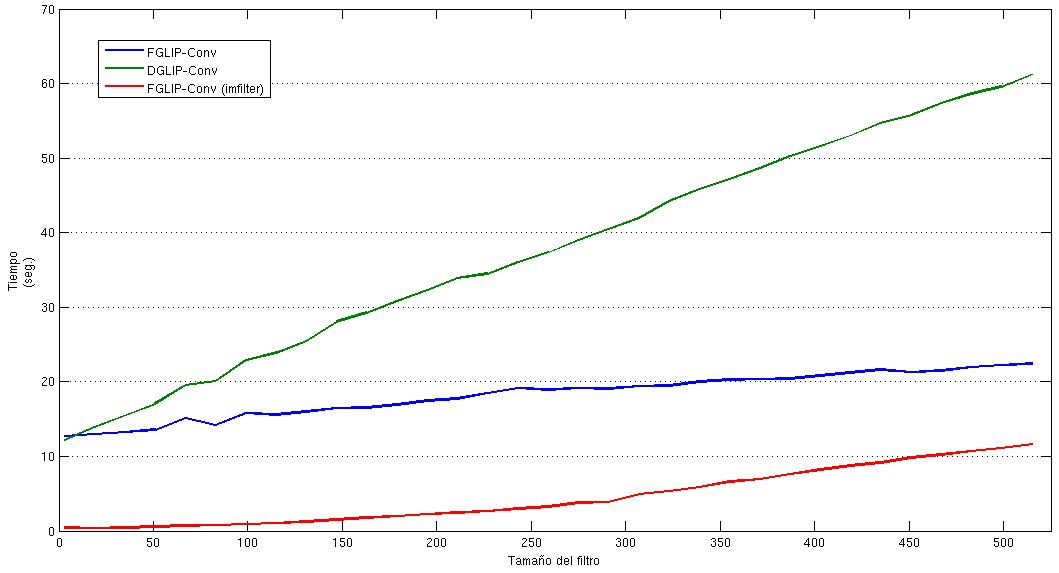
\includegraphics[width=26pc]{gfx/fg-dg}\caption[Comparativa FGLIP-Conv vs. DGLIP-Conv]{Comparativa de tiempos de FGLIP-Conv y DGLIP-Conv para distintos tama�os de filtros sobre una imagen de $1024 \times 1024$ p�xeles.}\label{fig:fg-dg}
% \end{SCfigure}
% \begin{SCfigure}[][!t]
% 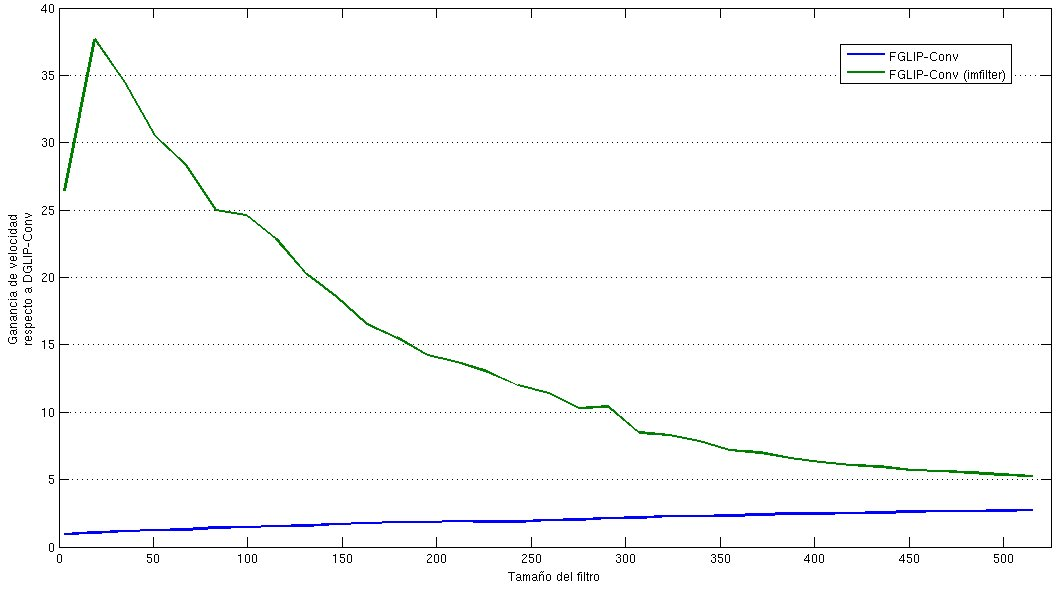
\includegraphics[width=26pc]{gfx/speedup-fg-dg}\caption[Speedup FGLIP-Conv vs. DGLIP-Conv]{Ganancia de velocidad de FGLIP-Conv frente a DGLIP-Conv para distintos tama�os de filtros sobre la misma imagen de $1024 \times 1024$ p�xeles.}\label{fig:speedup-fg-dg}
% \end{SCfigure}

\noindent Como se puede observar en la Fig. \ref{fig:fg-dg}, para todos los tama�os de filtros, \textsc{FGLIP--Conv} es mucho m�s r�pido que \textsc{DGLIP--Conv}. Tambi�n se puede apreciar en dicha gr�fica que la versi�n optimizada, \textsc{FGLIP--Conv Optim.} es mucho m�s r�pida que las otras dos implementaciones.\\
\noindent En la Fig. \ref{fig:speedup-fg-dg}, se muestra la ganancia de velocidad de \textsc{FGLIP--Conv} frente a \textsc{DGLIP--Conv}. La ganancia de la versi�n no optimizada, \textsc{FGLIP--Conv}, se encuentra en torno al $2\%$ de media. El aumento de la ganancia de velocidad es mucho mayor cuando se utiliza la versi�n \emph{Optimizada}, estando siempre por encima del $10\%$ y llegando a picos del $37\%$, aunque este rendimiento va degrad�ndose poco a poco conforme aumenta el tama�o del filtro. Por el contrario, \textsc{FGLIP--Conv} presenta un aumento suave pero progresivo en la ganancia de velocidad con respecto a los tiempos de \textsc{DGLIP--Conv}.
\subsection{Coste computacional por operador}
Para una misma ejecuci�n particular, se ha realizado un perfilado (\emph{profiling}) de cada l�nea de c�digo para cada una de las dos implementaciones descritas, obteni�ndose los resultados que se muestran en la Tab. \ref{tab:profiling}. En ella, se puede observar c�mo para la implementaci�n de \textsc{DGLIP--Conv}, el tiempo empleado en la exponenciaci�n es pr�cticamente igual a la suma del tiempo de todos los operadores utilizados en \textsc{FGLIP--Conv}. Esto demuestra que el coste computacional debido a los operadores es mucho mayor en \textsc{DGLIP--Conv}

\begin{SCtable}[][h]
\begin{tabular}{lcc}
\rowcolor{colorCorporativoSuave}
 Implementaci�n				& Operador		& Tiempo \\
\hline \hline
\rowcolor{colorCorporativoMasSuave}
\cellcolor{colorCorporativoMasSuave}	& Multiplicaci�n 	& 12.40  \\
\rowcolor{colorCorporativoSuave}
\multirow{-2}{*}{\cellcolor{colorCorporativoMasSuave}\textsc{FGLIP--Conv}} & Suma           	& 13.82  \\
\hline
\rowcolor{colorCorporativoMasSuave}
\cellcolor{colorCorporativoSuave}		& Multiplicaci�n 	& 15.77  \\
\rowcolor{colorCorporativoSuave}
\multirow{-2}{*}{\cellcolor{colorCorporativoSuave}\textsc{DGLIP--Conv}}& Exponenciaci�n 	& 22.07  \\
\hline
\end{tabular}\caption{Coste computacional por operador.}\label{tab:profiling}
\end{SCtable}
\section{Conclusiones}
\lettrine{E}{ste} cap�tulo, en el que se ha presentado toda la formulaci�n matem�tica para el desarrollo del operador \emph{Convoluci�n--\textsc{LIP}}, constituye el n�cleo principal de esta Tesis Doctoral. Este operador permite, de manera sencilla y homog�nea, adaptar una gran cantidad de algoritmos de procesamiento de im�genes y v�deo al paradima \textsc{LIP}.\\ 
\noindent Como resumen se muestran a continuaci�n las principales aportaciones cient�ficas obtenidas a partir de la investigaci�n desarrollada en este cap�tulo:
\begin{itemize}
\item \emph{Convoluci�n--\textsc{LIP}}: Se ha propuesto este nuevo operador dise�ado matem�ticamente utilizando la fortaleza y robustez que proporciona la estructura algebraica del paradigma \textsc{LIP}. Este dise�o matem�tico ha permitido construir dos implementaciones diferentes:
    \begin{aenumerate}
    \item \textsc{DGLIP--Conv}: Esta implementaci�n se obtiene a trav�s del m�todo ``directo'', utilizando las im�genes originales sin transformar y un conjunto de operadores matem�ticos modificados. Tras operar matem�ticamente se consigue una f�rmula que utiliza multiplicaciones y exponenciaciones.
    \item \textsc{FGLIP--Conv}: Parte del m�todo ``transformado'', que utiliza las im�genes aplic�ndoles una funci�n de transformaci�n y los operadores matem�ticos cl�sicos, multiplicaci�n y suma.
    \end{aenumerate}
\end{itemize}

\noindent Hay que indicar que ambas implementaciones son equivalentes en t�rminos de resultados, gracias a lo cual se tienen dos mecanismos diferentes para aplicar uno de los operadores m�s extendidos en el procesamiento de im�genes, como es la \emph{convoluci�n} bajo un modelo \textsc{LIP}. �ste posee unos beneficios muy importantes al trabajar con im�genes: coherencia de las operaciones con leyes f�sicas y psico--f�sicas, todas las operaciones \textsc{LIP} se mantienen dentro del rango de trabajo, los algoritmos presentan una cierta inmunidad ante efectos de iluminaci�n no homog�nea y muestran una mayor sensibilidad en zonas oscuras. A pesar de la equivalencia de las implementaciones, unos experimentos han mostrado que la implementaci�n \textsc{FGLIP--Conv} calcula la \emph{Convoluci�n--\textsc{LIP}} de manera m�s r�pida que la implementaci�n \textsc{DGLIP--Conv}.\\ 
\noindent La \emph{convoluci�n} es un operador que suele estar implementado y optimizado en diferentes arquitecturas de computaci�n, lo cual proporciona un mayor rendimiento que las implementaciones estr�ctamente software de dicho operador. Gracias a que \textsc{FGLIP--Conv} permite utilizar la \emph{convoluci�n} est�ndar, se ha mostrado que es posible construir dicho operador haciendo uso de la \emph{convoluci�n} optimizada presente en la mayor�a de sistemas de computaci�n, con un rendimiento a�n m�s eficiente que la versi�n que implementa la \emph{convoluci�n} a partir de sus operadores b�sicos.\\
\noindent En este cap�tulo se ha demostrado que el nuevo operador \emph{Convoluci�n--\textsc{LIP}} proporciona resultados que se encuentran siempre dentro del rango $(0,M)$, independientemente de los valores del filtro que se aplique. Esto tiene unas connotaciones muy importantes, al conocerse de antemano que la imagen resultante tras aplicar \emph{Convoluci�n--\textsc{LIP}} contendr� valores dentro de los rangos de visibilidad definidos. As� pues, no ser� necesario realizar comprobaciones de rangos de cada p�xel, ni normalizaciones o reajustes de rangos, muy habituales al aplicar muchos algoritmos en otros modelos. Todo ello significar� una reducci�n del tiempo de c�mputo necesario, adem�s de todas las ventajas que ofrece el modelo \textsc{LIP} para la aplicaci�n de algoritmos de procesamiento de im�genes y v�deo.

\myChapter{Criterios para la Evaluaci�n de la Calidad de Contornos}\label{chap:criterios}
\minitoc\mtcskip
\vfill
\lettrine{T}{odas} las t�cnicas nuevas que se proponen en la literatura cient�fica deben presentar una evaluaci�n de sus resultados, en la que el m�todo propuesto sea comparado con otros 
ya consolidados. Esta evaluaci�n termina reduci�ndose a uno o varios valores num�ricos, que sirven como resumen de la calidad general de dicho m�todo, y que se encuentran normalizados para poder compararlos con los de otras alternativas. En definitiva, el objetivo es determinar qu� t�cnica, m�todo o algoritmo es el \emph{mejor}.\\
\noindent Como se ha indicado en cap�tulos anteriores (ver Cap. \ref{chap:MOS} y \ref{chap:encuestas}), las t�cnicas de procesamiento de im�genes son susceptibles de ser evaluadas de manera subjetiva mediante el uso de cuestionarios de opini�n. Adem�s, en muchos casos, para evaluar la ``facilidad perceptual'' de un m�todo, los cuestionarios y la evaluaci�n subjetiva es la �nica opci�n. A lo largo de este cap�tulo se tratar�n diferentes aspectos de la evaluaci�n de las im�genes procesadas, mostrando la dificultad que presenta el desarrollo de los cuestionarios para su evaluaci�n subjetiva. Se seleccionar�n los diferentes \textsc{dominios} de las im�genes utilizados en el cuestionario y se elegir�n las diferentes im�genes representativas de cada uno de los mismos. Tambi�n se especificar�n los m�todos que se evaluar�n mediante cuestionarios.
\clearpage
\section{Objetivo principal y Criterios generales}\label{sec:objetivoCuestionario}
\lettrine{E}{n} el Cap�tulo \ref{chap:encuestas} se muestran dos listas de tareas que hay que seguir. En ellas, tanto \person{Burgess} \citep{burgess01} como \person{Oppenheim} \citep{oppenheim00}, indican como primer paso el de definir el prop�sito de la investigaci�n de opini�n. En la Tab. \ref{tab:objetivoCuestionario} se muestra  el objetivo principal de la investigaci�n de la presente Tesis Doctoral.
\begin{SCtable}[][!h]
\begin{tabular}{|A|}
\hline
Determinar si los m�todos de extracci�n de bordes basados en el paradigma \textsc{LIP} generan mapas de contornos de mayor calidad para aplicaciones de soporte visual humano que el resto de los m�todos de extracci�n de bordes.\vspace{1em}\\
\hline
\end{tabular}\caption[Objetivo del cuestionario]{Objetivo principal del estudio de investigaci�n.}\label{tab:objetivoCuestionario}
\end{SCtable}

\noindent Como se puede observar, el prop�sito del estudio de investigaci�n presenta t�rminos muy gen�ricos, que se ir�n acotando a continuaci�n.
\subsection{Criterios generales}\label{sec:criteriosGenerales}
Tras fijar el objetivo del estudio de investigaci�n, para que la evaluaci�n de los algoritmos de extracci�n de bordes sea eficaz, hay que fijar \apriori unos \emph{criterios}. En el Cap�tulo \ref{chap:MOS} se mostr� c�mo \person{Heath} \citep{heathMTh} propuso unos criterios para el proceso de evaluaci�n que realiz�, que son adaptables a cualquier otro proceso de evaluaci�n de algoritmos de procesamiento de im�genes. Dichos criterios, expuestos en la Tab. \ref{tab:criteriosGenerales} de la p�gina \pageref{tab:criteriosGenerales}, son los criterios generales que se han seguido en esta Tesis para dise�ar los cuestionarios para la evaluaci�n de algoritmos de extracci�n de bordes. En este trabajo tambi�n se han seguido esos criterios con car�cter general, puesto que est�n avalados por un proyecto de M�ster en una Universidad de prestigio \citep{heathMTh}, y por la publicaci�n de varios art�culos cient�ficos en congresos internacionales \citep{heath96} y en revistas de alto
impacto \citep{heath97,heath98}. A continuaci�n, se puntualizan todos aquellos aspectos espec�ficos que han sido de inter�s para el desarrollo del proceso de evaluaci�n.
%\newpage
\section{Criterios espec�ficos}\label{sec:criteriosEspecificos}
La primera precisi�n sobre la que hay que incidir es la determinaci�n del contexto en el que se trabaja, es decir, especificar la \emph{tarea de visi�n} en la que se miden las \emph{variables} estad�sticas que permiten alcanzar el \textsc{objetivo funcional} descrito en la Tab. \ref{tab:objetivoCuestionario}. Seg�n \person{Heath} \citep{heathMTh}, ``\emph{aunque se podr�a medir la calidad de los bordes fuera del contexto de una tarea de visi�n, los resultados obtenidos ser�an de dif�cil interpretaci�n en t�rminos de procesamiento de im�genes}''.
Por ello, para poder concretar la \emph{tarea de visi�n}, primero hay que estudiar qu� \textsc{dominios} se consideran dentro del cuestionario. Tras ello, se podr�n seleccionar los m�todos de extracci�n de bordes que se evaluar�n. Esto permitir� determinar el �mbito de actuaci�n para dicha evaluaci�n. Para ello, ser� necesario establecer las poblaciones objetivo y ajustar los par�metros visuales para que todos los m�todos se encuentren en situaciones de partida similares para su evaluaci�n.
\subsection{\textsc{Dominios} del cuestionario}\label{sec:dominiosCuestionario}
Ampliando los criterios propuestos por \person{Heath} \citep{heathMTh}, �ste afirma que ``\emph{un sistema de visi�n espec�fico se debe evaluar tomando un \textsc{dominio} particular y dicha evaluaci�n debe realizarse utilizando im�genes reales representativas del \textsc{dominio} particular en el que se pretende evaluar.}'' Para poder seleccionar las im�genes hay que determinar primero los \textsc{dominios} de los cuestionarios de evaluaci�n en el contexto de esta Tesis Doctoral.\\
\noindent Gran parte de esta tarea se ha realizado en el Cap�tulo \ref{sec:cuestionariosBajaVision}, en el que se preseleccionaron 7 \textsc{dominios}. Esta preselecci�n se ha realizado tomando en consideraci�n �nicamente aquellos \textsc{dominios} que son relevantes dentro de los cuestionarios de evaluaci�n de la \textsc{Baja Visi�n}, y que adem�s tienen utilidad dentro del �mbito de trabajo de los m�todos propuestos en esta Tesis.\\
\noindent De estas 7 \textsc{dimensiones} preseleccionadas, D4 (\emph{Sensibilidad y Adaptaci�n a la luz y problemas de iluminaci�n, deslumbramientos y Visi�n y Conducci�n nocturna}) es claramente un \textsc{dominio} transversal, ya que no es posible obtener im�genes exclusivamente de este tipo sin que est�n cruzadas con el resto de \textsc{dimensiones}.\\
\noindent Se descarta el \textsc{dominio} D2 (\emph{Agudeza visual en la Visi�n cercana, lectura de libros, peri�dicos, list�n telef�nico, escritura de cheques}), porque los requisitos y par�metros que deben tener los m�todos de extracci�n de contornos para este �mbito difieren mucho de las otras. Esto sugiere que este \textsc{dominio} representa una problem�tica independiente del resto, que deber�a ser enfocada de manera expl�cita y no conjuntamente. Adicionalmente, debido a las caracter�sticas propias de la tarea descrita (\emph{lectura y visi�n cercana}), �sta requiere una buena iluminaci�n sin sombras, aspecto este �ltimo que choca directamente con el \textsc{dominio} \emph{transversal} D4.\\
\noindent Continuando con el an�lisis, la \textsc{dimensi�n} D10 (\emph{Actividad principal: trabajo y tareas del hogar}) puede unificarse con la \textsc{dimensi�n} D8 (\emph{Cuidado personal: aseo, ba�o, comer}) en un nuevo \textsc{dominio}, que puede nombrarse como \emph{Visi�n cercana: Lectura y tareas b�sicas personales}.
\noindent Por tanto, de los 7 \textsc{dominios} preseleccionados en el Cap�tulo \ref{sec:cuestionariosBajaVision} se ha logrado reducir la lista a tan s�lo cinco \textsc{dominios}, que se muestran en la Tab. \ref{tab:dominiosCuestionario}. De ellos, los cuatro primeros permiten la obtenci�n de im�genes espec�ficas para cada uno de ellos, mientras que el quinto es transversal a todos los dem�s. Con esta reducci�n, se ha conseguido adem�s que todos los cuestionarios analizados en el Cap. \ref{sec:cuestionariosBajaVision} se encuentren representados en al menos uno de los \textsc{dominios} de la lista. En esta tabla tambi�n se incluye el nombre abreviado por el que se denominar�, por comodidad, cada \textsc{dominio}.
\begin{SCtable}[][!ht]
\begin{tabular}{|A|}
\hline
\begin{enumerate}
\item Visi�n cercana: Lectura y tareas b�sicas personales (\textsc{Dominio}
\texttt{cercanas}).
\item Visi�n media/larga distancia: Orientaci�n y seguridad en exteriores
(\textsc{Dominio} \texttt{exteriores}).
\item Visi�n media/larga distancia: Orientaci�n y seguridad en interiores
(\textsc{Dominio} \texttt{interiores}).
\item Visi�n media/larga distancia: Ubicaci�n y reconocimiento de personas
(\textsc{Dominio} \texttt{personas}).
\item Problemas de iluminaci�n, deslumbramientos y adaptaci�n a la luz.
(\emph{Transversal})
\end{enumerate}
\\
\hline
\end{tabular}\caption[Dominios seleccionados]{\textsc{Dominios} seleccionados
para el cuestionario de \textsc{Baja Visi�n}.}\label{tab:dominiosCuestionario}
\end{SCtable}
\FloatBarrier
\subsection{Contexto de las tareas de visi�n}
Por su naturaleza, las im�genes contienen una cantidad de informaci�n muy elevada, que el sistema visual humano se encarga de procesar desde los niveles m�s bajos (extracci�n de bordes, agrupamiento de texturas y colores, etc.) hasta abstracciones y connotaciones conceptuales de muy alto nivel, como pueden ser, asignaciones de percepciones psico--visuales (por ejemplo, saber si los colores de un determinado objeto son v�lidos) y/o culturales (por ejemplo, asociar conceptos positivos o negativos a s�mbolos). Esta gran cantidad de informaci�n subyacente en las im�genes hace que no todos los usuarios se fijen en los mismos aspectos al observar la misma imagen. Por ello es conveniente seleccionar una tarea de visi�n com�n, que permita al encuestador centrar la atenci�n visual en un aspecto concreto y espec�fico, lo que permite a los usuarios concentrarse en la acci�n encomendada y olvidarse de los otros est�mulos visuales presentes en las im�genes. As� pues, en la Tab. \ref{tab:tareasVision} se decriben las tareas t�picas de visi�n artificial \citep{bovik00,jahne02,gordon97,gonzalez02}.\\
\noindent Teniendo en cuenta los \textsc{dominios} expuestos en la Tab. \ref{tab:dominiosCuestionario} y las tareas de visi�n descritas en la Tab. \ref{tab:tareasVision} se puede concluir que el contexto de la tarea de visi�n de las preguntas del cuestionario debe ser la tarea general de \textsc{\person{Reconocimiento de Objetos}}, y de manera espec�fica, dependiendo de cada imagen en particular, la tarea concreta deber�a ser la de
\mbox{\textsc{\color{darkOrange}Detecci�n}}, \mbox{\textsc{\color{darkOrange}Reconocimiento}} o \mbox{\textsc{\color{darkOrange}Identificaci�n}}. Estas tres tareas est�n consideradas como los tres niveles progresivos del \textsc{\person{Reconocimiento de Objetos}}. Esta afirmaci�n se ve reforzada con el trabajo de \person{Abdou} y \person{Dusassoy} \citep{Abdou86}, en el que los observadores humanos que procesan las im�genes catalogan las tareas de \textsc{\person{Reconocimiento de Objetos}} en cuatro categor�as:
\mbox{\textsc{\color{darkOrange}Detecci�n}}, \mbox{\textsc{\color{darkOrange}Orientaci�n}}, \mbox{\textsc{\color{darkOrange}Reconocimiento}} e \mbox{\textsc{\color{darkOrange}Identificaci�n}}.
\begin{SCtable}[][!h]
\begin{tabular}{p{0.9\textwidth}}
\hline
\begin{aenumerate}
\item \textsc{\person{Reconocimiento de Objetos}}: \emph{Determinar si en una escena est� presente alg�n objeto espec�fico, alguna caracter�stica o alguna actividad concreta.}
\begin{description}
    \item[Detecci�n]\emph{B�squeda dentro de la imagen de alguna condici�n especial, por ejemplo, invasi�n de un carril por un veh�culo o b�squeda de c�lulas infectadas en una muestra.}
    \item[Orientaci�n]\emph{Detecci�n de alguna parte de un objeto que permita determinar, al menos, la orientaci�n de dicho objeto.}
    \item[Reconocimiento]\emph{Determinaci�n de la posici�n de un objeto gen�rico previamente ``aprendido''.}
    \item[Identificaci�n]\emph{Reconocimiento de una instancia espec�fica de un objeto, por ejemplo, una determinada cara o una huella dactilar.}
\end{description}
\item \textsc{\person{Estimaci�n del Movimiento}}: \emph{Mecanismo para estimar la velocidad relativa de los diversos objetos de una escena.}
\begin{description}
  \item[Seguimiento] \emph{Capacidad para rastrear los movimientos de un objeto en una escena (t�picamente, un veh�culo o una persona).}
  \item[Calibraci�n de c�mara] \emph{Determinaci�n del movimiento r�gido 3D de la c�mara que est� tomando las im�genes.}
\end{description}
\item \textsc{\person{Reconstrucci�n de escenas}}: \emph{Recreaci�n 3D de una escena a partir de varias im�genes 2D.}
\item \textsc{\person{Mejora de la calidad de las im�genes}}:
\begin{description}
  \item[Restauraci�n] \emph{Eliminaci�n de ruido, eliminaci�n de emborronamiento, etc.}
  \item[Mejora] \emph{T�cnicas que mejoran la calidad percibida de las im�genes: aumento del contraste, etc.}
\end{description}
\end{aenumerate}
\\
\hline
\end{tabular}\caption[Tareas t�picas de visi�n]{Tareas t�picas de visi�n artificial.}\label{tab:tareasVision}
\end{SCtable}
\subsection{Selecci�n de las t�cnicas de detecci�n de bordes}
Tomando la clasificaci�n expuesta en el Cap�tulo \ref{chap:ProcImagenes}, los m�todos para la extracci�n de bordes se dividen en tres grandes bloques:
\begin{itemize}
\item Basados en el Gradiente.
\item Basados en el Laplaciano.
\item Basados en operadores Morfol�gicos.
\end{itemize}
\noindent De los tres tipos de extractores, el �ltimo (\emph{basados en operadores Morfol�gicos}) no se ha contemplado en esta Tesis Doctoral, puesto que no utiliza el operador \emph{convoluci�n} y, por tanto, se aleja del planteamiento original del trabajo. Para poder realizar una evaluaci�n realista, se ha escogido un algoritmo representativo de cada uno de los bloques, y uno m�s adicional, el algoritmo de \emph{Canny}, que est� considerado como uno de los m�todos de m�s alta calidad para la extracci�n de contornos. Junto a estos, se han
tomado los respectivos algoritmos implementados bajo el paradigma \textsc{LIP}, descritos con mayor profundidad en el Cap. \ref{chap:aplicacionesConvLIP}.
\begin{SCtable}[][!h]
\begin{tabular}{|B|}
\hline
\rowcolor{colorCorporativoMasSuave}
\vspace{-0.5em}\begin{aenumerate}
\item Basado en el Gradiente:
\begin{enumerate}
\item \textsc{Sobel}.
\item \textsc{LIP--Sobel}.
\end{enumerate}
\item Basado en el Laplaciano:
\begin{enumerate}
\item \textsc{LoG}.
\item \textsc{LIP--LoG}.
\end{enumerate}
\item Alta precisi�n:
\begin{enumerate}
\item \textsc{Canny}.
\item \textsc{LIP--Canny}.
\end{enumerate}
\end{aenumerate}
\\
\hline
\end{tabular}\caption[T�cnicas seleccionadas]{T�cnicas seleccionadas para su evaluaci�n.}\label{tab:tecnicasSeleccionadas}
\end{SCtable}
\subsection{Selecci�n del �mbito de actuaci�n}
Como se ha expuesto con anterioridad, es necesario fijar el �mbito de actuaci�n para evaluar la calidad de las t�cnicas propuestas utilizando el paradigma \textsc{LIP}. Con esto se consigue fijar los objetivos que se desean medir en dicha evaluaci�n y que sirven para determinar la estructura y contenidos de la encuesta de opini�n que se utilizar� para evaluar la calidad de dichas t�cnicas. En este �mbito, se presentan dos objetivos principales, mostrados en la Tab. \ref{tab:objetivosEncuesta}, que se desean contrastar mediante la evaluaci�n subjetiva.

\begin{SCtable}[][!h]
\begin{tabular}{|B|}
\hline
\rowcolor{colorCorporativoMasSuave}
\vspace{-0.5em}\begin{aenumerate}                                                                                                              
\item Los m�todos desarrollados bajo \textsc{LIP} presentan un mejor comportamiento para la detecci�n de objetos en sombras para usuarios sin problemas particulares de visi�n.
\item Los pacientes con \textsc{Baja visi�n} prefieren las im�genes obtenidas con los m�todos desarrollados bajo \textsc{LIP} frente a las obtenidas con los m�todos tradicionales.
\end{aenumerate}
\\
\hline
\end{tabular}\caption[Objetivos principales de la encuesta]{Objetivos principales de la encuesta.}\label{tab:objetivosEncuesta}
\end{SCtable}

\noindent Los estudios de investigaci�n mediante cuestionarios necesitan identificar las poblaciones de individuos a los que se les realizar�n las preguntas\hfill de\hfill los\hfill cuestionarios.\hfill Como\hfill se\hfill puede\hfill observar\hfill del\hfill estudio\hfill de\\
\clearpage
\noindent los objetivos principales, cada uno de ellos tiene una poblaci�n de inter�s diferente, por lo que se pueden detectar dos grupos poblacionales claramente diferenciados, que se muestran en la Tab. \ref{tab:gruposPoblacionales}.

\begin{SCtable}[][!h]
\begin{tabular}{|B|}
\hline
\rowcolor{colorCorporativoMasSuave}
\vspace{-0.5em}\begin{aenumerate}
\item Usuarios con nivel de \textsc{Visi�n Est�ndar}.
\item Pacientes con \textsc{Baja visi�n}.
\end{aenumerate}
\\
\hline
\end{tabular}\caption[Grupos poblacionales de la encuesta]{Tipolog�as de grupos poblacionales de la encuesta.}\label{tab:gruposPoblacionales}
\end{SCtable}

\subsection{Selecci�n de los par�metros visuales}
Para que las comparaciones entre los diversos algoritmos se puedan realizar en t�rminos de igualdad, todos los algoritmos y m�todos deben proporcionar bordes de similar grosor y calidad. Como elemento de normalizaci�n, en esta Tesis Doctoral, se ha incorporado a todas las t�cnicas un mecanismo de supresi�n de bordes no maximales y de posterior hist�resis de contornos. Por �ltimo, en todos los m�todos se ha decidido aplicar un filtrado morfol�gico final para obtener im�genes de bordes con caracter�sticas homog�neas. Estas caracter�sticas se muestran en la Tab. \ref{tab:parametrosVisuales}.
\begin{SCtable}[][!h]
\begin{tabular}{|B|}
\hline
\rowcolor{colorCorporativoMasSuave}
\vspace{-0.5em}\begin{aenumerate}
\item Todos los bordes deben tener 1 p�xel de grosor.
\item Deben detectarse �nicamente p�xeles de bordes no esp�reos.
\end{aenumerate}
\\
\hline
\end{tabular}\caption{Caracter�sticas homog�neas de todos los m�todos evaluados en la encuesta.}\label{tab:parametrosVisuales}
\end{SCtable}
                                                                                                                                                                                                                                                                                                             
\noindent Para la detecci�n de bordes es necesario establecer un umbral que determine si el valor procesado de un determinado p�xel es considerado borde o no. La selecci�n de dicho umbral es un aspecto delicado, puesto que una mala selecci�n del umbral puede provocar un resultado p�simo en la evaluaci�n. Adem�s, aunque en la literatura cient�fica no se ha encontrado ning�n trabajo que indique la cantidad m�xima de contornos que podr�a admitir un usuario para no verse saturado, los pacientes con \textsc{Baja Visi�n} informan que es preferible una menor cantidad de bordes antes que una alta precisi�n de los mismos. De manera heur�stica, mediante ensayos realizados por un conjunto de expertos en la materia, se ha estimado que el porcentaje m�ximo de contornos ha
de ser, en todo caso, menor a un $20 \%$ de los p�xeles totales de la imagen. Utilizando este porcentaje, para cada imagen, se determinar� un valor del umbral, de tal manera, que el n�mero de p�xeles de bordes seleccionados en la imagen sea menor a dicho porcentaje. As� pues, los par�metros se ajustar�n teniendo en cuenta las caracter�sticas indicadas en la Tab. \ref{tab:umbrales}.
\begin{SCtable}[][!h]
\begin{tabular}{|B|}
\hline
\rowcolor{colorCorporativoMasSuave}
\vspace{-0.5em}\begin{aenumerate}
\item El n�mero de p�xeles de contornos en el mapa final se debe mantener en valores porcentuales bajos ($\le 20\%$) en relaci�n con el tama�o de la imagen.
\item Un experto realizar� la selecci�n del valor exacto del umbral.
\end{aenumerate}
\\
\hline
\end{tabular}\caption[Determinaci�n de umbrales]{Determinaci�n de umbrales.}\label{tab:umbrales}
\end{SCtable}
\section{Im�genes para el cuestionario de evaluaci�n en \textsc{Baja visi�n}}
\lettrine{L}{a} selecci�n de las im�genes utilizadas en el cuestionario se ha
realizado en funci�n de los \textsc{dominios} seleccionados previamente (ver
Tab. \ref{tab:dominiosCuestionario}). Inicialmente se ha partido de un total de
114 im�genes de distintos \textsc{dominios}:
\begin{itemize}
\item \textsc{Visi�n Cercana}: 32 im�genes.
\item \textsc{Orientaci�n en interiores}: 24 im�genes.
\item \textsc{Orientaci�n en exteriores}: 39 im�genes.
\item \textsc{Reconocimiento de personas}: 19 im�genes.
\end{itemize}

\noindent Estas im�genes provienen de bancos de im�genes p�blicas, o bien, han sido tomadas por el propio autor de esta Tesis. Cada una de estas im�genes presenta un elemento principal que permite catalogarla dentro de uno de los \textsc{dominios}. Adem�s, todas las im�genes seleccionadas contienen \emph{iluminaci�n} no uniforme, sombras u otras caracter�sticas propias del \textsc{dominio} transversal expuesto en la Tab.\ref{tab:dominiosCuestionario}.\\
\noindent Utilizando esta primera selecci�n de im�genes, se han aplicado las diferentes t�cnicas seleccionadas previamente (\emph{Sobel, \textsc{LIP}--Sobel, LoG, \textsc{LIP}--LoG, Canny, \textsc{LIP}--Canny}) con las restricciones de los par�metros previamente indicadas (\emph{4 niveles de porcentaje: 5\%, 10\%, 15\% y 20\% de contornos en las im�genes}), gener�ndose un conjunto de 2736 im�genes de bordes.\\
\noindent Todas estas im�genes de bordes han sido analizadas por expertos en procesamiento de im�genes, para descartar todas aquellas que no proporcionan resultados aceptables (por exceso de ruido o por insuficiencia de contornos), reduciendo el conjunto de im�genes originales a 20, con un l�mite de 5 im�genes por \textsc{dominio}. Las Figuras \ref{fig:personas1} a \ref{fig:exteriores5} muestran el conjunto reducido de im�genes originales utilizado para generar las im�genes de bordes del cuestionario de evaluaci�n. Todas estas im�genes est�n disponibles en: \url{http://www.uco.es/users/el2pamuj/research/LowVision/}.
\begin{SCfigure}[][!t]
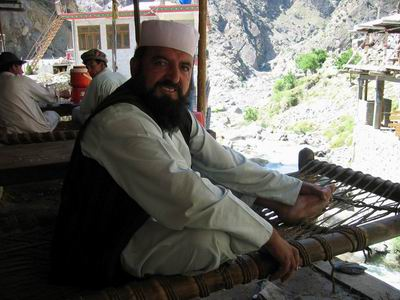
\includegraphics[width=21pc]{gfx/afgano}\caption[Imagen Personas 1]{Imagen 1
original del \textsc{dominio} \texttt{personas}.\label{fig:personas1}}
\end{SCfigure}
\begin{SCfigure}[][!t]
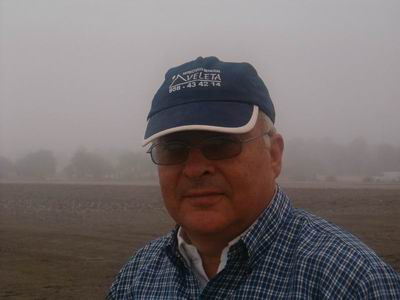
\includegraphics[width=21pc]{gfx/cara-gorra}\caption[Imagen Personas 2]{Imagen 2
original del \textsc{dominio} \texttt{personas}.\label{fig:personas2}}
\end{SCfigure}

\begin{SCfigure}[][!t]
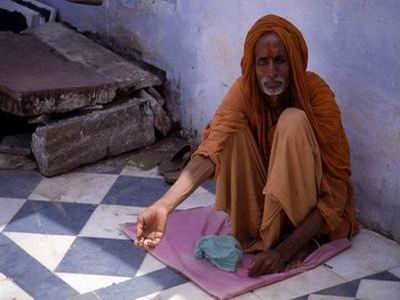
\includegraphics[width=21pc]{gfx/hombre_pidiendo}\caption[Imagen Personas
3]{Imagen 3 original del \textsc{dominio}
\texttt{personas}.\label{fig:personas3}}
\end{SCfigure}

\begin{SCfigure}[][!t]
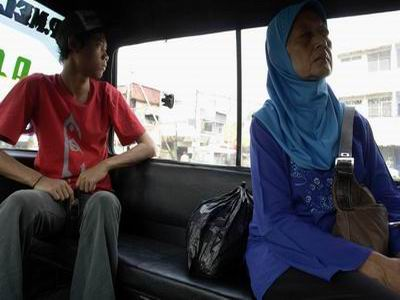
\includegraphics[width=21pc]{gfx/microlet}\caption[Imagen Personas 4]{Imagen 4
original del \textsc{dominio} \texttt{personas}.\label{fig:personas4}}
\end{SCfigure}

\begin{SCfigure}[][!t]
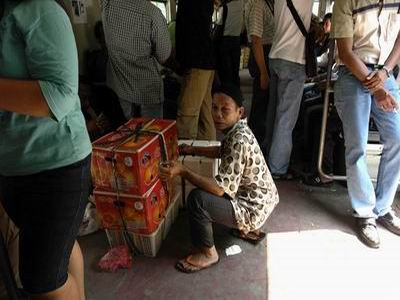
\includegraphics[width=21pc]{gfx/vendedor-sombras}\caption[Imagen Personas
5]{Imagen 5 original del \textsc{dominio}
\texttt{personas}.\label{fig:personas5}}
\end{SCfigure}

\clearpage

\begin{SCfigure}[][!t]
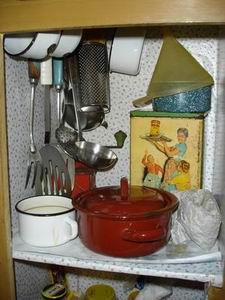
\includegraphics[width=16pc]{gfx/alacena}\caption[Imagen Cercanas 1]{Imagen 1
original del \textsc{dominio} \texttt{cercanas}.\label{fig:cercanas1}}
\end{SCfigure}

\begin{SCfigure}[][!t]
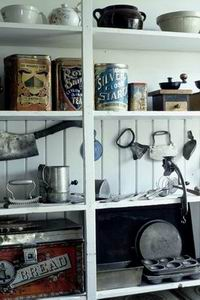
\includegraphics[width=16pc]{gfx/despensa}\caption[Imagen Cercanas 2]{Imagen 2
original del \textsc{dominio} \texttt{cercanas}.\label{fig:cercanas2}}
\end{SCfigure}

\begin{SCfigure}[][!t]
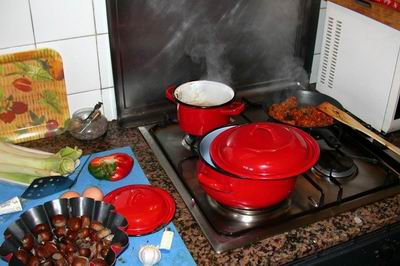
\includegraphics[width=21pc]{gfx/cocina}\caption[Imagen Cercanas 3]{Imagen 3
original del \textsc{dominio} \texttt{cercanas}.\label{fig:cercanas3}}
\end{SCfigure}

\begin{SCfigure}[][!t]
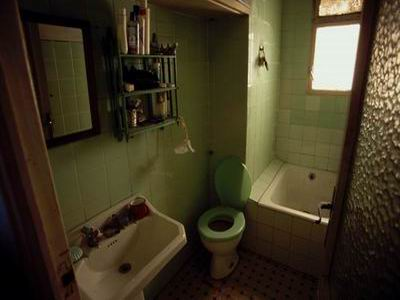
\includegraphics[width=21pc]{gfx/lavabo}\caption[Imagen Cercanas 4]{Imagen 4
original del \textsc{dominio} \texttt{cercanas}.\label{fig:cercanas4}}
\end{SCfigure}

\clearpage

\begin{SCfigure}[][!t]
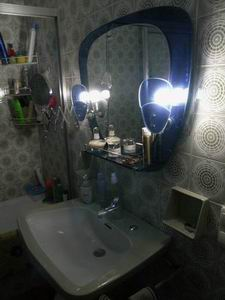
\includegraphics[width=16pc]{gfx/lavabo1}\caption[Imagen Cercanas 5]{Imagen 5
original del \textsc{dominio} \texttt{cercanas}.\label{fig:cercanas5}}
\end{SCfigure}

\begin{SCfigure}[][!t]
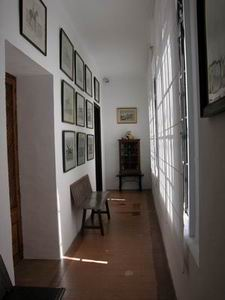
\includegraphics[width=16pc]{gfx/pasillo-cuadros2}\caption[Imagen Interiores
1]{Imagen 1 original del \textsc{dominio}
\texttt{interiores}.\label{fig:interiores1}}
\end{SCfigure}

\begin{SCfigure}[][!t]
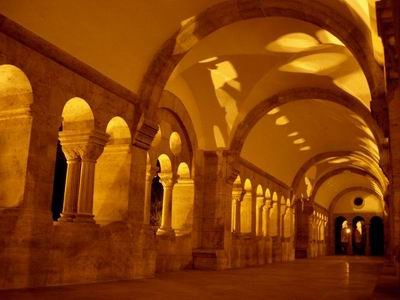
\includegraphics[width=21pc]{gfx/galeria-budapest}\caption[Imagen Interiores
2]{Imagen 2 original del \textsc{dominio}
\texttt{interiores}.\label{fig:interiores2}}
\end{SCfigure}

\begin{SCfigure}[][!t]
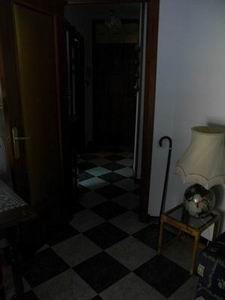
\includegraphics[height=21pc]{gfx/pasillo1-noluz}\caption[Imagen Interiores
3]{Imagen 3 original del \textsc{dominio}
\texttt{interiores}.\label{fig:interiores3}}
\end{SCfigure}

\begin{SCfigure}[][!t]
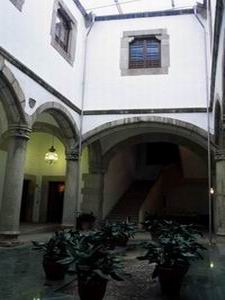
\includegraphics[width=16pc]{gfx/patio-sombras}\caption[Imagen Interiores
4]{Imagen 4 original del \textsc{dominio}
\texttt{interiores}.\label{fig:interiores4}}
\end{SCfigure}

\begin{SCfigure}[][!t]
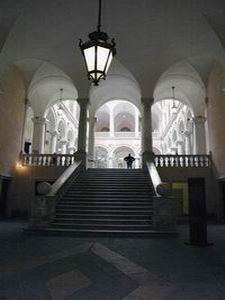
\includegraphics[width=16pc]{gfx/escaleras-sombras}\caption[Imagen Interiores
5]{Imagen 5 original del \textsc{dominio}
\texttt{interiores}.\label{fig:interiores5}}
\end{SCfigure}

\begin{SCfigure}[][!t]
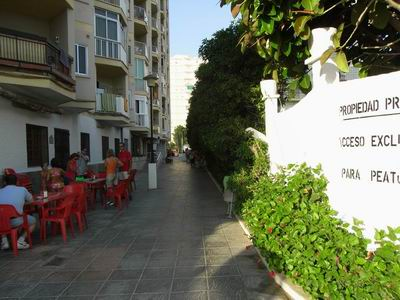
\includegraphics[width=21pc]{gfx/bares}\caption[Imagen Exteriores 1]{Imagen 1
original del \textsc{dominio} \texttt{exteriores}.\label{fig:exteriores1}}
\end{SCfigure}

\begin{SCfigure}[][!t]
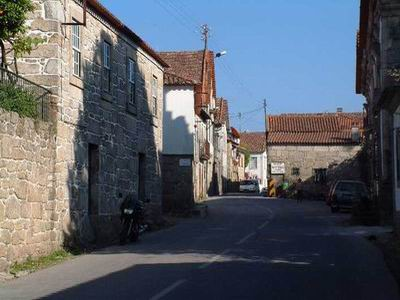
\includegraphics[width=21pc]{gfx/calle-sombra5}\caption[Imagen Exteriores
2]{Imagen 2 original del \textsc{dominio}
\texttt{exteriores}.\label{fig:exteriores2}}
\end{SCfigure}

\begin{SCfigure}[][!t]
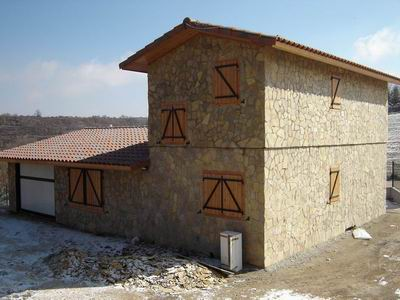
\includegraphics[width=21pc]{gfx/casa}\caption[Imagen Exteriores 3]{Imagen 3
original del \textsc{dominio} \texttt{exteriores}.\label{fig:exteriores3}}
\end{SCfigure}

\clearpage

\begin{SCfigure}[][!t]
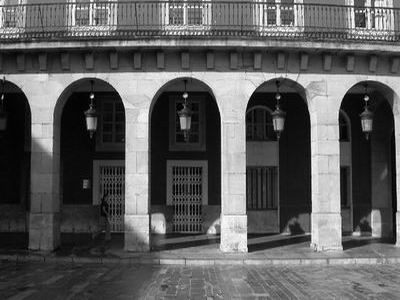
\includegraphics[width=21pc]{gfx/soportalesOriginal}\caption[Imagen Exteriores
4]{Imagen 4 original del \textsc{dominio}
\texttt{exteriores}.\label{fig:exteriores4}}
\end{SCfigure}

\begin{SCfigure}[][!t]
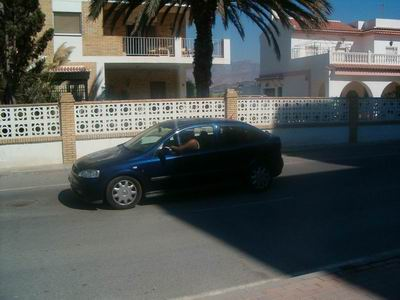
\includegraphics[width=21pc]{gfx/coche2}\caption[Imagen Exteriores 5]{Imagen 5
original del \textsc{dominio} \texttt{exteriores}.\label{fig:exteriores5}}
\end{SCfigure}

\clearpage
\newpage

\section{Conclusiones}
\lettrine{E}{n} este cap�tulo se han mostrado tanto los objetivos generales como los espec�ficos utilizados para el dise�o de los experimentos y de los cuestionarios para evaluar los resultados. El objetivo principal del estudio de investigaci�n es determinar \emph{si los m�todos de extracci�n de bordes basados en el paradigma \textsc{LIP} generan mapas de contornos de mayor calidad para aplicaciones de soporte visual humano que el resto de los m�todos de extracci�n de bordes}. Para lo cual, se obtendr�n im�genes de bordes, que ser�n evaluadas por humanos. Este proceso lleva a tomar algunas decisiones de dise�o m�s espec�ficas. Primero, se han estudiado los cuestionarios de evaluaci�n de \textsc{Baja Visi�n} y mediante un exhaustivo proceso de an�lisis y s�ntesis, se
han  seleccionado 4 \textsc{dominios} espec�ficos, entre los que se escoger�n las im�genes para los experimentos, y un \textsc{dominio} transversal, que afecta al resto de \textsc{dominios}. Los \textsc{dominios} seleccionados se muestran en la Tab. \ref{tab:dominiosCuestionario}.\\
\noindent Para evaluar la calidad de las im�genes de bordes, los encuestados deben realizar una cierta \emph{tarea de visi�n} utilizando como entrada im�genes procesadas, pertenecientes a los distintos \textsc{dominios}. Sobre cada imagen de bordes, se solicita a los encuestados que realice una determinada
\emph{tarea de visi�n}:
\begin{itemize}
\item \textsc{Detecci�n} de objetos.
\item \textsc{Reconocimiento} de objetos.
\item \textsc{Identificaci�n} de objetos.
\end{itemize}

\noindent En la Tab. \ref{tab:tecnicasSeleccionadas} se muestran los algoritmos de extracci�n de bordes que
se han seleccionado para la evaluaci�n mediante cuestionarios.\\                                                                            
\noindent Tambi�n se han especificado los par�metros visuales comunes a todos los m�todos que se evaluar�n. Estos par�metros permitir�n comparar, con caracter�sticas normalizadas y homog�neas, los resultados de todos los algoritmos de extracci�n de bordes, sin favorecer ni perjudicar ninguno de los m�todos evaluados. Los par�metros comunes seleccionados se muestran en las Tab. \ref{tab:parametrosVisuales} y \ref{tab:umbrales}.\\
\noindent La evaluaci�n de la calidad de los contornos generados por estos algoritmos bajo estos par�metros se realiza en dos �mbitos, mostrados en la Tab. \ref{tab:objetivosEncuesta}. Estos representan los objetivos funcionales primarios de la encuesta.\\
\noindent La cumplimentaci�n de estos objetivos se realizar� por 2 grupos poblacionales diferenciados: 
\begin{itemize}
\item Usuarios con nivel de \textsc{Visi�n Est�ndar}.
\item Pacientes con \textsc{Baja visi�n}.
\end{itemize}

\noindent Para finalizar, se han mostrado las 20 im�genes seleccionadas, con 5 im�genes de cada uno de los cuatro \textsc{dominios}.

\subsection{Contexto del cap�tulo} \noindent Tras exponer en el cap�tulo anterior el nuevo operador \emph{Convoluci�n--\textsc{LIP}}, en �ste se han expuesto los criterios generales y espec�ficos que permiten el desarrollo de los algoritmos de extracci�n de bordes bajo el modelo \textsc{LIP}, con los que se realizar�n los experimentos y la evaluaci�n de los mismos.\\
\noindent Como se ha comentado a lo largo de la Tesis Doctoral, la evaluaci�n se realiza mediante cuestionarios. Sin embargo, al no existir una metodolog�a para el dise�o de cuestionarios sobre calidad de im�genes procesadas, la construcci�n de este tipo de encuestas no es trivial. En cap�tulos posteriores, se proponen un conjunto de recomendaciones generales para el dise�o de cuestionarios que involucren contenidos multimedia, gracias al cual se podr�n construir encuestas que permitan catalogar, seg�n su calidad visual, los m�todos de extracci�n de bordes.
\myChapter{Recomendaciones para el Dise�o de Cuestionarios de Calidad de Contornos} \label{chap:recCuestCalidadBordes} \minitoc\mtcskip
\vfill
\lettrine{M}{uchos} autores indican que no es posible proporcionar un �nico e infalible conjunto de reglas, protocolos o metodolog�as para la correcta construcci�n o dise�o de cuestionarios, que eliminen completamente todo tipo de sesgo. En general, lo que se proponen son recomendaciones en el dise�o de las preguntas y de los cuestionarios para minimizar dicho sesgo. Como se ha indicado en cap�tulos anteriores, existen algunas recomendaciones de dise�o en el plano ling\"{u}�stico para la realizaci�n de cuestionarios. Sin embargo, no existen recomendaciones para cuestionarios en los que se incluyan elementos multimedia.\\
\noindent Se inicia identificando el nuevo \emph{sesgo por finalidad} y describiendo algunas recomendaciones para mitigar su efecto. Se contin�a aportando algunas recomendaciones de dise�o para cuestionarios que involucren preguntas con elementos visuales, y en particular, para la evaluaci�n subjetiva de la calidad de algoritmos de extracci�n de contornos. Para finalizar este cap�tulo, se presenta una herramienta Web para la creaci�n y difusi�n de los cuestionarios, que permite contestarlos \mbox{on--line}, y que facilita al investigador la recolecci�n de las respuestas.
\clearpage
\section{Sesgo por finalidad}\label{sec:sesgo-finalidad}
\lettrine{E}{l} \emph{Sesgo por finalidad} se produce cuando los encuestados conocen los objetivos asociados a la pregunta que est�n respondiendo y, por tanto, las respuestas pueden estar influenciadas por ello. En algunos casos, el efecto producido por el \emph{Sesgo de deseabilidad social} es similar, puesto que los encuestados no contestan seg�n sus opiniones propias, sino las que los encuestados creen que son las que mayor aprobaci�n social tendr�n. En cierto modo, los encuestados escogen las opciones influenciados por lo que ellos creen que el entrevistador desea que ellos contesten. En estos casos, las recomendaciones de dise�o indican que las preguntas que puedan sufrir de alg�n tipo de \emph{Sesgo de deseabilidad social} deben hacerse en un tono neutral y mediante preguntas indirectas, de tal forma que sea m�s complicado percibir la intencionalidad (los objetivos subyacentes asociados) de dichas preguntas.\\
Las encuestas que tratan de estimar la calidad de alg�n proceso suelen depender de la finalidad con la que se aplique dicho proceso. Es decir, que un mismo proceso puede proporcionar un resultado muy positivo para una aplicaci�n determinada, y muy negativo para otras. Por ejemplo, un medicamento puede ser muy eficaz para tratar una enfermedad y, a la vez, estar contraindicado para otras. Este sesgo puede aparecer en diferentes escenarios: cuando el entrevistado conoce (directamente informado por el entrevistado o porque ha sido capaz de deducirlo) la finalidad del proceso sobre el que se le est� encuestando, o cuando cree conocer dicha finalidad y realmente se confunde a s�� mismo, proporcionando respuestas totalmente err�neas. Normalmente, suele estar causado por una incorrecta redacci�n de las preguntas por parte del entrevistador, no dejando claramente especificada la finalidad de cada pregunta.\\
\noindent En el caso de las encuestas de calidad, en muchos casos hay que guiar al encuestado sobre qu� debe observar o analizar, proporcion�ndole en estos casos el objetivo de la pregunta. Por ejemplo, si en una cata ciega de un nuevo producto se desea que los usuarios den su opini�n sobre un determinado aspecto del mismo, habr��a que indicarles que se deben centrar en un aspecto en particular, ya que no se desea conocer otros aspectos de ese producto. Concretando el ejemplo, si el producto fuese una bebida, se podr��a preguntar en exclusiva sobre el dulzor, la acidez, la textura, etc. Sin embargo, puede que ese aspecto en particular no sea el que m�s llame la atenci�n a los encuestados, o incluso, que si no se le hubiese preguntado espec��ficamente por �l, habr��a pasado desapercibido. En estos casos, aunque los encuestados proporcionen las respuestas basadas en su propia opini�n, �stas est�n influidas por el \emph{Sesgo por finalidad}.\\
\noindent En la mayor��a de los casos en los que aparece este tipo de sesgo, �ste se introduce debido a que el dise�ador de la encuesta necesita indicar a los encuestados el objetivo que se est� buscando en cada pregunta, para centrar la atenci�n de los encuestados en dicho aspecto, descartando otros elementos presentes en dicha pregunta. Se plantean dos posibilidades:
\begin{aenumerate}
\item No informar a los encuestados de la finalidad de cada pregunta, permitiendo que las respuestas de los encuestados no se ajusten a los objetivos de cada pregunta.
\item Informar a los encuestados de la finalidad en cada pregunta, asumiendo que se est� introduciendo este tipo de sesgo en todas las preguntas.
\end{aenumerate}

\noindent Con la primera posibilidad, se elimina el \emph{Sesgo por finalidad}, ya que se est� omitiendo la informaci�n de la finalidad de las preguntas, por lo que no se influye a los encuestados. Sin embargo, no hay garant��a de que los encuestados proporcionen respuestas que sirvan para contestar a los objetivos asociados a cada pregunta.\\
\noindent Por el contrario, con la segunda posibilidad se introduce expl��citamente este sesgo en todas las preguntas. De esta manera se reduce la libertad de los encuestados en las posibles respuestas, pero se intenta garantizar un nivel de conocimiento base que permita a los encuestados proporcionar respuestas que sean interesantes para el evaluador en el contexto para el que ha desarrollado la pregunta. Esta segunda opci�n es admisible si se informa a todos los encuestados de los objetivos de cada una de las preguntas del cuestionario. No es conveniente mezclar en un mismo cuestionario preguntas en las que se indique el objetivo de las mismas con otras preguntas en las que esto no se indique, ya que, al estar m�s guiadas unas respuestas que otras, los resultados no son comparables.

\section{Recomendaciones generales sobre las preguntas}
\lettrine{C}{on} los cuestionarios indicados en esta Tesis se intenta evaluar de manera subjetiva qu� algoritmo de procesamiento de im�genes se comporta de mejor manera ante un determinado entorno de funcionamiento (que viene determinado por los \textsc{Dominios} del cuestionario). A continuaci�n, se muestra la estructura que se recomienda que tenga un cuestionario.
\subsection{Estructura de las preguntas}
Se considera que un cuestionario est� compuesto por una o varias preguntas; y cada pregunta est� compuesta por:

\begin{aenumerate}
\item Un texto de introducci�n y de pregunta.
\item Una imagen original [Optativa].
\item Una o varias \emph{im�genes respuesta}, cada una con su zona de respuesta asociada.
\end{aenumerate}

\noindent Se ha considerado que lo m�s eficiente para este tipo de cuestionarios es no mezclar preguntas que contengan elementos visuales con preguntas de tipo exclusivamente ling\"{u}�stico. Si se mezclan ambos tipos de preguntas, la evaluaci�n se complica mucho para el entrevistador. Como se ver� m�s adelante, cada pregunta tiene ponderada su contribuci�n al resultado final, y conseguir dicho factor de ponderaci�n en preguntas exclus�vamente ling\"{u}�sticas es muy complejo. Adem�s, se han realizado diversas pruebas con cuestionarios experimentales (pruebas de pilotaje inicial), que han mostrado que los entrevistados mostraban mayores dificultades al responder cuestionarios con mezcla de ambos tipos de preguntas (ling\"{u}�sticas y visuales) que los cuestionarios con preguntas de un �nico tipo. Los entrevistados argumentaron que les ``costaba'' ir cambiando de formato de pregunta cuando ya se hab�an acostumbrado a responder preguntas de un determinado tipo.
\subsection{Im�genes respuesta}
Las \emph{im�genes respuesta} son las distintas im�genes de respuesta asociadas a cada pregunta, donde se busca que el entrevistado responda a la cuesti�n planteada en el ``texto de introducci�n y de pregunta''. En dicho texto se solicita al entrevistado que realice alguna tarea de visi�n (\textsc{detecci�n}, \textsc{orientaci�n}, \textsc{reconocimiento} o \textsc{identificaci�n}) utilizando en cada caso la \emph{imagen respuesta} correspondiente. Cada una de ellas tendr� asociado un �nico algoritmo de procesamiento de im�genes.
\subsection{Ponderaci�n de preguntas}
No todas las preguntas tienen el mismo valor para obtener el resultado final, puesto que hay algunas preguntas que pueden ser discriminatorias, mientras que otras pueden matizar el grado de especializaci�n. T�mese como ejemplo, una pregunta en la que se solicite que se indiquen aquellas \emph{im�genes respuesta} en las que se pueda detectar un determinado objeto, sin importar si se detecta mejor o peor. Todas aquellas \emph{im�genes respuesta} en las que no sea apreciable dicho objeto obtendr�n baja puntuaci�n, y por lo tanto, los algoritmos de procesamiento de im�genes asociados a esas \emph{im�genes respuesta} conseguir�n pocos puntos. Pero adem�s, desde un punto de vista global, esa pregunta es altamente discriminatoria, es decir, que para la puntuaci�n global de los algoritmos de procesamiento de im�genes, existe una gran diferencia en el grado de colaboraci�n en la puntuaci�n final de los casos en los que los entrevistados pueden detectar el objeto frente a los casos en los que no pueden detectarlo. Por tanto, cada pregunta colaborar� con el resultado final con un cierto grado, especificado utilizando valores de ponderaci�n, que podr�n variar seg�n las distintas clases de respuestas posibles.\\
\noindent A pesar de que este comportamiento es altamente deseable, una ponderaci�n de todas las preguntas de un cuestionario que sea satisfactoria y que no presente ni \emph{sesgo} ni favorezca \apriori ning�n m�todo es muy dif�cil de conseguir. Para poder simplificar la tarea del dise�o de la encuesta, en esta Tesis Doctoral no se aplicar�n distintas ponderaciones, sino que todas las preguntas colaborar�n en la misma proporci�n en el c�lculo del resultado final.
\clearpage
\section{Tipos de preguntas con elementos visuales}
\lettrine{L}{os} posibles tipos de preguntas que se consideran en los cuestionarios de calidad de bordes en im�genes son los de:

\begin{aenumerate}
\item Preguntas con respuestas de \textsc{selecci�n} (o \textsc{dicot�micas}).
\begin{aenumerate}
    \item \textsc{Con repetici�n} (Varias \emph{im�genes respuesta} v�lidas).
    \item \textsc{Sin repetici�n} (S�lo una \emph{imagen respuesta} v�lida).
\end{aenumerate}
\item Preguntas con respuestas de \textsc{puntuaci�n}.
\begin{aenumerate}
    \item \textsc{Con repetici�n} (Varias \emph{im�genes respuesta} pueden tener la misma puntuaci�n).
    \item \textsc{Sin repetici�n} (Cada \emph{imagen respuesta} tiene una puntuaci�n, y dicha puntuaci�n no ha sido asignada a ninguna otra imagen respuesta).
\end{aenumerate}
\item Preguntas con respuestas de \textsc{ordenamiento}.
\begin{aenumerate}
    \item \textsc{Con repetici�n} (Varias \emph{im�genes respuesta} pueden tener el mismo valor de asignaci�n).
    \item \textsc{Sin repetici�n} (Cada \emph{imagen respuesta} tiene un valor �nico de ordenamiento).
\end{aenumerate}
\item Preguntas con respuesta de \textsc{mapeado espacial y temporal} (o \textsc{Mapping}).
\end{aenumerate}

\subsection{Preguntas de \textsc{selecci�n} o \textsc{dicot�micas}}
Mediante este tipo de preguntas se busca encontrar en cu�les de las \emph{im�genes respuesta} el entrevistado puede realizar la tarea de visi�n encomendada en el texto de la pregunta. Para desambiguar cualquier posible duda que pudiera tener el entrevistado, el entrevistador debe especificar con la mayor claridad posible en el texto de la pregunta en qu� casos puede el entrevistado seleccionar la \emph{imagen respuesta} en funci�n de la realizaci�n de la tarea de visi�n (por ejemplo, si puede realizar perfectamente la tarea de visi�n encargada sin ninguna dificultad, o en otro caso distinto, si puede realizar al menos m�nimamente la tarea de visi�n aunque con un cierto grado de dificultad, etc.).
\paragraph{Sin repetici�n} \noindent Utilizando el mecanismo \textsc{sin repetici�n}, el entrevistador consigue un beneficio directo: obliga al entrevistado a escoger s�lo una de las \emph{im�genes respuesta}, a pesar de que quiz�s �ste pudiera realizar la tarea de visi�n encomendada en varias de ellas. El principal handicap que comentan los entrevistados sobre esta opci�n es que es poco natural, debido a que les fuerza a escoger, a�n cuando no lo desean. Un beneficio adicional que se consigue con este mecanismo es que �ste se puede considerar un selector elitista, es decir, que permite discriminar con mayor claridad cu�l es considerado el ``mejor'' algoritmo (asociado a una \emph{imagen resultado}), ya que �ste obtiene toda la puntuaci�n, mientras que el resto no obtiene ning�n punto.
\paragraph{Con repetici�n} \noindent Por el contrario, el mecanismo \textsc{con repetici�n} permite un mayor grado de libertad al entrevistado, ya que �ste no tiene que escoger s�lo una \emph{imagen respuesta}. Esta opci�n es mucho m�s natural, ya que si no existen excesivas diferencias entre los resultados de los distintos algoritmos que se est�n evaluando, es mucho m�s realista para un entrevistado afirmar que es capaz de realizar una determinada tarea de visi�n con varias \emph{im�genes respuesta} similares. Sin embargo, al contrario que en el mecanismo anterior, �ste permite una menor discriminaci�n al obtener igual puntuaci�n varios de los algoritmos (pudiendo incluso seleccionar todas las \emph{im�genes respuesta}).
\subsection{Preguntas de \textsc{puntuaci�n}}
Gracias a estas preguntas, el entrevistador puede conocer el grado de calidad intr�nseca percibida por los entrevistados asociada a la utilizaci�n de cada \emph{imagen respuesta} para realizar una tarea de visi�n (especificada en el ``texto de la pregunta'').\\
\noindent La utilizaci�n de varias im�genes permite a los entrevistados compararlas, por lo que en esos casos, la puntuaci�n que se asigne se puede considerar m�s como el grado de comparaci�n entre las im�genes que como la evaluaci�n individual de cada una. Al permitirse la comparaci�n entre las im�genes, los entrevistados incorporan m�s informaci�n al puntuar cada imagen que la incluida en la propia imagen, ya que pueden mirar el resto. En muchos casos, la puntuaci�n de cada \emph{imagen respuesta} se realiza valorando cada imagen con una imagen ``virtual'' que cada entrevistado se construye de manera heur�stica en su propia mente utilizando informaci�n visual de cada \emph{imagen respuesta}. Por tanto, en las preguntas que se utilicen m�s de una \emph{imagen respuesta} el entrevistador debe admitir la existencia de un cierto grado de \emph{sesgo por finalidad}, que debe ser minimizado mediante la inclusi�n de otras preguntas en las que no se muestren m�ltiples \emph{im�genes respuesta}.
\paragraph{Sin repetici�n} \noindent Utilizando el mecanismo \textsc{sin repetici�n}, el entrevistador fuerza a los entrevistados a asignar diferente puntuaci�n a todas las \emph{im�genes respuesta}. Si la puntuaci�n es un valor real, esta opci�n no tiene utilidad pr�ctica, por la facilidad que existe para modificar la puntuaci�n decimal. Por el contrario, si es un valor entero, se provoca una cierta distanciaci�n entre las \emph{im�genes respuesta}, lo que permite una mayor discriminaci�n en las respuestas. Sin embargo, esa diferenciaci�n puede ser totalmente ficticia, en el sentido que los entrevistados pueden encontrar una diferencia entre las \emph{im�genes respuesta} menor que la que le obliga la asignaci�n sin repetici�n y con valores enteros.
\paragraph{Con repetici�n} \noindent Por el contrario, el mecanismo \textsc{con repetici�n} permite una mayor flexibilidad a los entrevistados para asignar puntuaci�n. Al permitir la repetici�n, a veces, los entrevistados tienden a agrupar puntuaciones, es decir, asignan la misma puntuaci�n a todas las \emph{im�genes respuesta} que tienen una calidad elevada, sin precisar si en alguna de ellas la calidad es mayor o menor.
\subsection{Preguntas de \textsc{ordenamiento}}
Gracias a estas preguntas, el entrevistador puede conocer el orden de calidad percibida comparada por los entrevistados asociada a la utilizaci�n de cada \emph{imagen respuesta} para realizar una tarea de visi�n (especificada en el ``texto de la pregunta''). Como su propio nombre indica, el entrevistado ``ordena'' de mejor a peor las im�genes, asignando un valor num�rico a cada \emph{imagen respuesta} que permite organizarlas comparativamente. Con este tipo de preguntas, el entrevistador no tiene garant�a de que el entrevistado haya sido capaz de realizar la tarea de visi�n solicitada: s�lo se solicita que ordene de mejor a peor las \emph{im�genes respuesta}, cuando quiz�s el entrevistado no haya sido capaz de realizar la tarea encomendada, aunque de manera subjetiva es capaz de indicar con cu�l se siente m�s c�modo.\\
\noindent Se puede afirmar que este tipo de preguntas es menos exigente para el entrevistado que las de \textsc{puntuaci�n}, ya que al no tener que puntuar, no tiene que comparar mentalmente cada \emph{imagen respuesta} con la \emph{imagen respuesta} ``perfecta'' (que, previamente, el entrevistado se habr� formado en su mente); le basta con ordenar las existentes. Debido a la simplificaci�n en la evaluaci�n, este tipo de preguntas no proporcionan resultados excesivamente discriminantes. Un cuestionario realizado exclusivamente con este tipo de preguntas s�lo proporcionar�a \emph{tendencias} generales y para obtener resultados m�s concretos, estas preguntas se deben formular a�adidas a otras de otros tipos.
\paragraph{Sin repetici�n} \noindent Utilizando el mecanismo \textsc{sin repetici�n}, el entrevistador obliga que el entrevistado no pueda indicar que dos o m�s \emph{im�genes respuesta} son iguales o tienen la misma calidad para realizar la ``tarea de visi�n''. Este aspecto incrementa ligeramente la discriminaci�n, pero los entrevistados suelen mostrarse molestos por tener que escoger entre uno en particular y se pueden producir peque�os \emph{sesgos} con respecto a la posici�n de las \emph{im�genes respuesta} entre las que tiene que escoger (existiendo una leve preferencia hacia las que se encuentran a la izquierda, probablemente por ser la tendencia natural de la escritura occidental, de izquierda a derecha).
\paragraph{Con repetici�n} \noindent Por el contrario, el mecanismo \textsc{con repetici�n} permite mayor libertad a los entrevistados para clasificar las \emph{im�genes respuesta}, a costa de que dichas respuestas suelen tener menor discriminaci�n que el tipo anterior.

\subsection{Preguntas de \textsc{mapeado espacial y temporal}}
Mediante este tipo de preguntas, el entrevistador puede comprobar la precisi�n espacial y el tiempo que tardan los entrevistados en realizar las ``tareas de visi�n'' encomendadas. Estas preguntas, tambi�n llamadas de \textsc{Mapping}, s�lo admiten una \emph{imagen respuesta}, sobre la cual el entrevistado debe marcar en la posici�n en la que el propio entrevistado estima que se encuentra la caracter�stica solicitada en el texto de la pregunta. El entrevistador deber� tener se�alado en una copia propia de la \emph{imagen respuesta}, que no mostrar�a en ning�n caso al entrevistado, la posici�n exacta de la caracter�stica buscada, a lo que se ha dado en denominar \emph{punto} (o \emph{zona}) \emph{objetivo}. El encuestador podr� se�alar zonas de precisi�n, es decir, zonas alrededor del \emph{punto objetivo} que podr�n tener distinta ponderaci�n. Mediante esta opci�n se controla la precisi�n espacial. En el caso de que la caracter�stica buscada sea marcable de manera puntual, bastar� con que el entrevistado se�ale dicho punto (por ejemplo, con el puntero del rat�n). Si la caracter�stica fuese una zona, el entrevistado tendr�a que marcar varios puntos que delimitasen dicha zona, para lo cual el sistema (si fuese por computador) podr�a facilitar el trabajo del entrevistado permitiendo el manejo autom�tico de estructuras poligonales. Esta opci�n, sin embargo, presenta un inconveniente que es el manejo de los errores (�reas que se encuentren fuera de la zona marcada por el entrevistador como \emph{zona objetivo}).\\
\noindent En muchas aplicaciones, la precisi�n espacial es importante, pero dentro de unos l�mites temporales. Es decir, existen situaciones en las que el entrevistado deber�a responder antes de un cierto tiempo, a partir del cual, la consideraci�n de la respuesta podr�a estar muy degradada o incluso puede no ser aceptable en absoluto (a pesar de que la misma fuese perfecta en cuanto a la precisi�n espacial). Para controlar esta opci�n el sistema debe controlar el tiempo de respuesta de los entrevistados ante la presentaci�n del est�mulo (la \emph{imagen respuesta}). En estos casos, se debe mostrar el texto de la pregunta a los entrevistados manteniendo la \emph{imagen respuesta} oculta hasta que �ste indique que est� preparado y se empiece a contar el tiempo. El encuestador debe tener una funci�n matem�tica que permita ponderar el tiempo de respuesta del entrevistado.\\
Utilizando este tipo de preguntas, el encuestador puede cruzar datos con otras preguntas y comprobar si realmente los entrevistados est�n realizando la ``tarea de visi�n'' encomendada. Esto permite controlar incorrecciones por parte de los encuestados. Por ejemplo, en otros tipos de preguntas, los entrevistados podr�an afirmar que son capaces de detectar un cierto objeto en una determinada \emph{imagen respuesta}, y sin embargo, al proponerles que se�alen donde se encuentra dicho objeto mediante una pregunta de \textsc{Mapping}, el entrevistado se�ala en otra zona distinta o no con demasiada precisi�n, o tarda mucho tiempo en determinar la posici�n exacta. Esto significar�a que la respuesta que dieron a la otra pregunta no era demasiado veraz, y por tanto, habr�a que tener mucha cautela al incluir dichas respuestas en el c�lculo final.\\
\noindent El principal inconveniente que presenta este tipo de preguntas es que s�lo se pueden evaluar una \emph{imagen respuesta} cada vez. Tambi�n hay que indicar que son un poco m�s dif�ciles y algo m�s tediosas de contestar que el resto.\\
\noindent Para finalizar, se ha de indicar que este tipo de preguntas se presenta como una aportaci�n especial de esta Tesis, y se ha dise�ado haciendo uso espec�fico del soporte inform�tico, aunque con algunas peque�as adaptaciones podr�a utilizarse en encuestas ``en papel''.
\clearpage
\section{Recomendaciones sobre la estructura general del cuestionario}
A continuaci�n, se analizan algunos aspectos que tienen una influencia en el dise�o del cuestionario y se propondr�n una serie de recomendaciones sobre la estructura del cuestionario. La mayor�a de estas recomendaciones intentan reducir el \emph{sesgo} que el uso de contenidos visuales puede introducir en el cuestionario en general y en cada pregunta en particular.\\
\subsection{Reutilizaci�n de im�genes}
Uno de los primeros aspectos que se consideran cuando se dise�a un cuestionario con contenidos visuales, es la reutilizaci�n de esos mismos contenidos visuales. Esta reutilizaci�n se presenta en dos vertientes, utilizar exactamente las mismas \emph{im�genes respuesta}, obtenidas utilizando el mismo m�todo de procesamiento de im�genes con los mismos par�metros, o bien, utilizar la misma imagen original y obtener diferentes \emph{im�genes respuesta} (ya sea variando el m�todo de procesamiento de im�genes, modificando los par�metros aplicados o ambos casos) que son representaciones visuales de la misma imagen original.\\
\noindent Se ha podido observar que los entrevistados \emph{recuerdan} las caracter�sticas de las im�genes reutilizadas, produci�ndose un \emph{sesgo} en la respuesta de los mismos. Para comprobar este comportamiento se realiz� un experimento en los que los entrevistados ten�an que puntuar la calidad de los mapas de bordes de ciertas \emph{im�genes respuesta}. El cuestionario estaba compuesto por 5 preguntas. En cada pregunta se aplicaba un mismo m�todo de procesamiento de bordes sobre la misma imagen original, variando los par�metros de dicho m�todo, obteniendo las \emph{im�genes respuesta} que se comparaban en cada pregunta.\graffito{La reutilizaci�n de im�genes fomenta el \emph{recuerdo} de las mismas.} Sin conocimiento de los entrevistados, la primera pregunta y la �ltima pregunta del cuestionario eran id�nticas y mostraban exactamente las mismas \emph{im�genes respuesta}, incluyendo el mismo orden de presentaci�n de las mismas. Se pudo observar que todos los entrevistados respondieron de manera an�loga en la primera y en la �ltima pregunta, sin embargo, en general tardaron mucho menos en contestar la �ltima pregunta que la primera, a pesar de que eran iguales. Tras finalizar la encuesta, se les pregunt� porqu� hab�an tardado menos en responder a la �ltima pregunta que a la primera y todos ellos respondieron que ``\emph{ya conoc�an las im�genes}''.\\
\noindent En el caso de uso de preguntas con respuestas de \textsc{mapeado espacial y temporal}, d�nde tanto la precisi�n de la respuesta como el tiempo de respuesta influyen en la calidad de la misma, la reutilizaci�n de im�genes es un elemento cr�tico. Si utilizando este tipo de preguntas se pretende evaluar la calidad de varios m�todos o del mismo m�todo con diferentes par�metros, es imprescindible utilizar la misma imagen original. Para estudiar la influencia de la reutilizaci�n de la misma imagen original en preguntas con respuestas de \textsc{mapeado espacial y temporal}, se realiz� un peque�o estudio mediante un cuestionario compuesto �ntegramente por preguntas de \textsc{Mapping} en las que se utilizaban \emph{im�genes respuesta} que part�an de la misma imagen orignal con diferentes m�todos de procesamiento de im�genes. En todas las preguntas de \textsc{Mapping} se solicitaba a los encuestados que marcasen d�nde consideraban que se encontraba un cierto objeto. Se pudo observar que la precisi�n espacial de los entrevistados mejoraba conforme iban respondiendo a m�s preguntas que utilizaban la misma imagen original, casi independientemente del grado de calidad de la \emph{imagen respuesta}. Es decir, al ir respondiendo preguntas, las respuestas iban aumentando la precisi�n espacial, siempre que el m�todo de extracci�n de bordes obtuviese algunos contornos del objeto que se buscaba, sin necesidad de que el contorno del objeto se hubiese obtenido completamente. Se pudo observar un comportamiento interesante y es que en cuanto los entrevistados contestaban a alguna pregunta en la que el contorno del objeto estuviese completo, en todas las preguntas posteriores la precisi�n espacial de la respuesta era muy elevada. Se puede decir, que en cuanto consegu�an encontrar el objeto por primera vez, ya lo encontraban siempre.\\
\noindent M�s evidente fue el an�lisis del tiempo de respuesta,\graffito{El tiempo de b�squeda en preguntas de \textsc{Mapping} con im�genes repetidas se va reduciendo conforme se contestan m�s preguntas con la misma imagen original.} en el que se pudo observar como dicho tiempo de respuesta se reduc�a al responder m�s preguntas, llegando a ser casi constante en las �ltimas, pr�cticamente sin influencia de la calidad de la \emph{imagen respuesta} que se mostrase. Se puede afirmar que los entrevistados recordaban la zona de la imagen d�nde se encontraba el objeto y no ten�an que volver a buscarlo por toda la imagen. Tambi�n, se puede indicar que el proceso de b�squeda y detecci�n se realizaba cada vez de manera m�s autom�tica por parte de los encuestados tras responder a m�s preguntas que se basan la misma imagen original.\\
\noindent Por tanto, si se reutilizan im�genes en preguntas con respuestas de \textsc{mapeado espacial y temporal}, ?`cu�ntas preguntas con otras im�genes diferentes hay introducir entre medio para que los entrevistados \emph{olviden} la imagen? Para responder a esta pregunta, se realiz� un experimento que determin� que, dos preguntas de \textsc{Mapping} que se basen en la misma imagen original deben estar separadas, al menos, por otras 3 preguntas y, a ser posible, que dichas preguntas no sean del mismo tipo, sino que sean otros diferentes (\textsc{selecci�n}, \textsc{puntuaci�n}, etc.).
\subsection{Uso de im�genes reales}
El uso de im�genes reales permite a los entrevistados comparar cada \emph{imagen respuesta} con la imagen real a partir de la cual se han generado. Utilizando las im�genes reales, los entrevistados obtienen mayor informaci�n visual, lo que permite en muchos casos eliminar algunas ``dudas''. Sin embargo, al presentar las im�genes reales, existe un elevado riesgo de introducir \emph{sesgo por finalidad}. Esto es debido a que el entrevistado deja de comparar �nicamente las \emph{im�genes respuesta} entre s�, para primero comparar cada una de ellas con la imagen real y, despu�s, comparar las \emph{im�genes respuesta} entre s�. Mediante este proceso de comparaci�n en dos pasos, el entrevistado, de manera consciente o no, tiende a \textsc{rellenar} zonas sensibles en las \emph{im�genes respuesta} que, en caso de no tener la imagen original, descartar�a (o aceptar�a, dependiendo de cada entrevistado).\\
\noindent En pruebas preliminares realizadas, se ha podido determinar que existe una cierta influencia en la respuesta de los entrevistados seg�n la presencia o no de la imagen original, es decir, que los entrevistados respond�an de forma ligeramente diferente ante las mismas \emph{im�genes respuesta} dependiendo de si se inclu�a la imagen original en la pregunta. En particular, se realiz� un experimento con dos cuestionarios sobre un grupo de entrevistados en los que en el primer cuestionario se les solicitaba que puntuasen la calidad de un grupo de \emph{im�genes respuesta} presentando para cada pregunta en dicho cuestionario las im�genes originales. En el segundo cuestionario, se les solicitaba que puntuasen las mismas \emph{im�genes respuesta} sin mostrarles las im�genes originales. Este segundo cuestionario, se les present� varios d�as despu�s para fomentar el \emph{olvido} de las im�genes por parte de los entrevistados y alterando el orden de las preguntas. Los cambios en las respuestas de los encuestados entre los dos cuestionarios se produjeron generalmente en las \emph{im�genes respuesta} de calidad intermedia, ya que las de alta calidad, siguieron obteniendo altas puntuaciones; al igual que las de baja calidad, que siguieron puntu�ndose de manera muy baja. Sin embargo, en las \emph{im�genes respuesta} de calidad intermedia se observ� un comportamiento no generalizable, hab�a entrevistados que aumentaban la puntuaci�n asignada anteriormente, mientras que otros entrevistados redujeron la puntuaci�n de la misma imagen. Por tanto, se podr�a afirmar que el uso de im�genes reales ayuda a los entrevistados a decidir con mayor informaci�n visual, pero que dicha informaci�n visual no es tratada de igual manera por todos los usuarios y por lo tanto, el comportamiento no es reproducible en todos los casos.
\subsection{N�mero de \emph{im�genes respuesta} por pregunta}
?`Cu�ntas \emph{im�genes respuesta} como m�ximo se deber�an utilizar en cada pregunta? Para contestar a esta pregunta se realiz� una encuesta de pilotaje con un grupo cerrado de 6 encuestados con un grado de \textsc{Visi�n Est�ndar} y 1 con \textsc{Baja Visi�n} por cataratas. En dicha encuesta se pusieron diferentes preguntas con distinto n�mero de \emph{im�genes respuesta}. Se incluyeron preguntas de \textsc{puntuaci�n} y \textsc{selecci�n}, tanto \textsc{sin repetici�n} como \textsc{con repetici�n}. Tras contestar la encuesta, a los encuestados se les realiz� una entrevista personal en la que se les pregunt� por el n�mero de \emph{im�genes respuesta} e indicaron que depend�a del tipo de pregunta. La apreciaci�n de la mayor�a (incluyendo la respuesta de la persona con \textsc{Baja Visi�n}) fue:
\begin{itemize}
\item Preguntas de \textsc{puntuaci�n} (\textsc{con} o \textsc{sin repetici�n}): Menos de 8 im�genes.
\item Preguntas de \textsc{selecci�n sin repetici�n}: Menos de 4 im�genes.
\item Preguntas de \textsc{selecci�n con repetici�n}: Entre 4 y 6 im�genes.
\item Preguntas de \textsc{Mapping}: No aplicable.
\end{itemize}
\noindent Los entrevistados indicaron, para cada caso, que m�s \emph{im�genes respuesta} les exig�a mucho esfuerzo para responder ya que ten�an que comparar muchas im�genes entre s�. Por el contrario, con un menor n�mero de ellas no hab�a suficientes donde escoger y sent�an un cierto grado de \emph{frustraci�n} al tener que seleccionar im�genes con las que no estaban totalmente de acuerdo.
%\clearpage
\section{Sistema Web para cuestionarios multimedia}
\lettrine{C}{omo} ya se ha expuesto en el Cap�tulo \ref{chap:encuestas}, hay dos tipos de cuestionarios seg�n el mecanismo de recolecci�n de respuestas: \emph{entrevistas estructuradas} y \emph{cuestionarios auto--administrados}. Para la evaluaci�n de la calidad de bordes, lo ideal ser�a realizar \emph{entrevistas estructuradas}. Sin embargo, la gran dificultad que se presenta para la ubicaci�n de pacientes con \textsc{Baja Visi�n} en un �nico sitio para poder realizar las entrevistas hace que este m�todo no sea factible. Por el contrario, el mecanismo de \emph{cuestionarios auto--administrados} presenta m�s virtudes para la evaluaci�n de calidad de bordes, ya que permite que los usuarios puedan parar y continuar la evaluaci�n seg�n sus propios intereses.\graffito[-7.5em]{Los pacientes con \textsc{Baja Visi�n} suelen presentar cansancio visual cuando realizan tareas visualmente exigentes.}\\
\noindent De manera habitual, los \emph{cuestionarios auto--administrados} se han realizado utilizando el soporte papel: se entrega un \emph{cuadernillo} que contiene las preguntas y una o varias \emph{hojas de respuesta}, en las que cada entrevistado se encarga de valorar las preguntas seg�n unas determinadas escalas. En general, la cumplimentaci�n de los cuestionarios es en muchos casos una tarea ardua para el entrevistado, ya que tiene que seleccionar unas respuestas a un determinado n�mero de preguntas, pasar correctamente dichas respuestas a la hoja de respuestas para el procesamiento estad�stico posterior por parte del encuestador, etc. Este proceso suele provocar el rechazo de los encuestados cuando son muchas preguntas o cuando el proceso de selecci�n de respuestas es complejo, por lo tedioso de la tarea. Debido a todo esto, en muchos casos, los encuestados abandonan las encuestas sin contestarlas. Otro aspecto que involucra el uso del soporte papel y que hay que tener en cuenta es tanto la cantidad de papel como de tintas que se utiliza, en muchos casos para un �nico uso.
\begin{SCfigure}[][t]
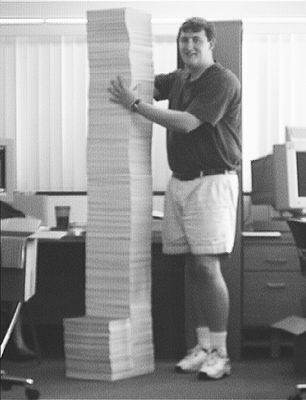
\includegraphics[width=18pc]{gfx/heath-encuestas}\caption[Encuestas trabajo Heath]{Imagen extra�da de \textsc{Heath} \etal \citep{heathMTh}, muestra las 19600 hojas de evaluaci�n impresas de todas las encuestas realizadas.\label{fig:heath-encuesta}}
\end{SCfigure}
\noindent Este uso desmesurado de papel y de tinta es muy poco ecol�gico, por su efectos contaminantes sobre el medio ambiente. Todos estos efectos se acent�an en cuestionarios con im�genes, ya que dichas im�genes han de imprimirse en alta calidad y en alg�n tipo de papel fotogr�fico o, en cualquier caso, de mayor grosor que el papel habitual, y con una gran cantidad de tinta de varios  colores. Tampoco es posible el uso de papel reciclado, ya que los colores y la resoluci�n se ven afectados en este tipo de papel. Todos estos aspectos elevan el coste final del cuestionario. Como ejemplo, en la Fig. \ref{fig:heath-encuesta} se muestra al autor de \citep{heathMTh} fotografiado junto con una columna de papel impreso correspondiente a las 19600 p�ginas de todas las encuestas realizadas para dicho trabajo. Esta imagen muestra gr�ficamente y de manera muy evidente el enorme gasto tanto en papel como en costes de impresi�n que conlleva una evaluaci�n mediante cuestionarios impresos. Adicionalmente, a este tipo de evaluaci�n hay que incorporar otros costes, como es el tiempo empleado en recopilar las respuestas y transcribirlas a una base de datos para su posterior procesamiento.\\
\noindent Frente a la aproximaci�n basada en la impresi�n en papel de los cuestionarios, se encuentra la cumplimentaci�n de los cuestionarios utilizando alg�n sistema Web. La alta calidad de los monitores, con elevadas resoluciones gr�ficas, y la disponibilidad de los cuestionarios en todo momento y en todo sitio con conexi�n a Internet, hacen que los sistemas Web se postulen como una buena soluci�n para enfrentarse a la evaluaci�n de encuestas de tipo multimedia. Por todo lo anterior, para proporcionar soporte a los cuestionarios para la evaluaci�n de la calidad de distintas t�cnicas de procesamiento de im�genes se ha planificado un sistema Web.\\
\noindent Siguiendo las recomendaciones expuestas en este cap�tulo se ha desarrollado una herramienta que permite el dise�o de cuestionarios para la evaluaci�n de contenidos multimedia. A su vez, este sistema facilita la gesti�n de dichos cuestionarios tanto por parte del encuestador para su tratamiento, como de los encuestados para contestarlos. Finalmente, proporciona al encuestador la evaluaci�n de los resultados de los cuestionarios tras aplicarles diversos factores de ponderaci�n.\\
\noindent Esta herramienta ha sido implementada como un sistema Web, para permitir que los encuestados puedan acceder de manera remota a los cuestionarios. De manera adicional, los usuarios pueden interrumpir y retomar los cuestionarios en cualquier momento. Esto es una pr�ctica bastante com�n en pacientes con problemas de visi�n debido al cansancio visual que les acarrea el esfuerzo de ver las im�genes.
\clearpage
\subsection{Preguntas de \textsc{puntuaci�n}}
En la Fig. \ref{fig:wemcas-puntuacion} se muestra un ejemplo de pregunta de \textsc{puntuaci�n} de una encuesta de pilotaje para la evaluaci�n de bordes.\\
\begin{SCfigure}[][!h]
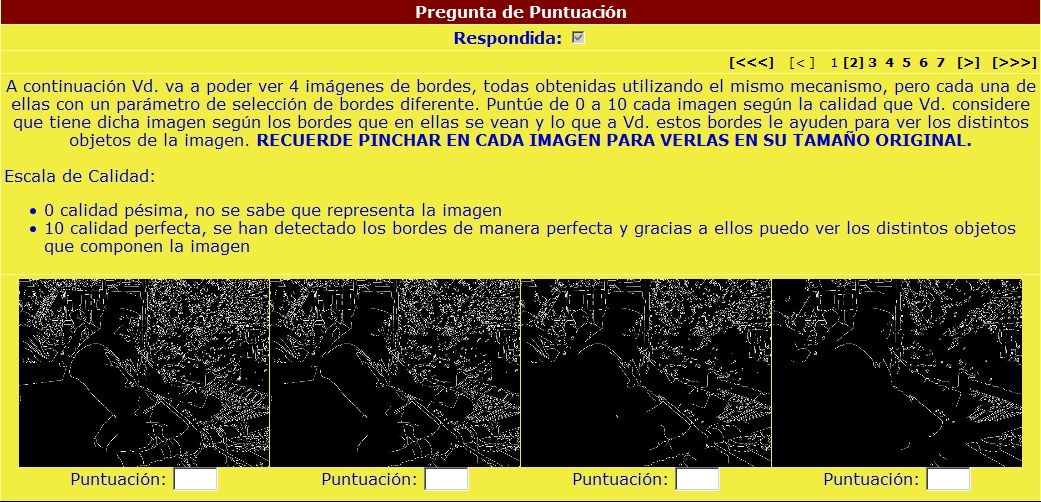
\includegraphics[width=26pc]{gfx/wemcas/wemcas-puntuacion.jpg}\caption[Pregunta de \textsc{puntuaci�n}]{Pregunta de \textsc{puntuaci�n con repetici�n}.\label{fig:wemcas-puntuacion}}
\end{SCfigure}

\noindent N�tese que debajo de cada \emph{imagen respuesta} existe una caja de texto que admite un valor num�rico. Los l�mites inferior y superior de dicho valor se puede parametrizar por parte del encuestador cuando construye el cuestionario, de manera que impida la introducci�n de valores fuera de rango.

\subsection{Preguntas de \textsc{selecci�n sin repetici�n}}
En la Fig. \ref{fig:wemcas-seleccion-unica} se muestra un ejemplo de pregunta de \textsc{selecci�n sin repetici�n} de una encuesta de pilotaje para la evaluaci�n de bordes.
\begin{SCfigure}[][!h]
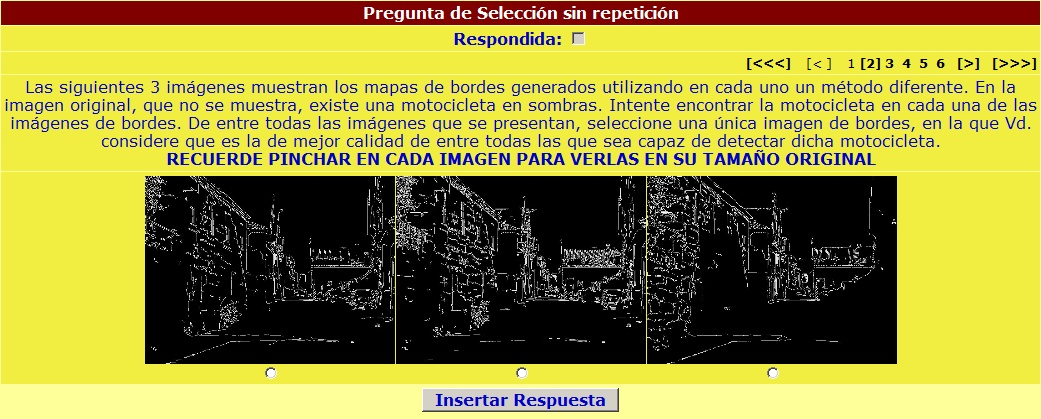
\includegraphics[width=26pc]{gfx/wemcas/wemcas-seleccion-unica.jpg}\caption[Pregunta de \textsc{selecci�n sin repetici�n}]{Pregunta de \textsc{selecci�n sin repetici�n}.\label{fig:wemcas-seleccion-unica}}
\end{SCfigure}

\noindent Debajo de cada \emph{imagen respuesta} hay un bot�n circular que muestra si se ha seleccionado la imagen superior asociada y que, a su vez, s�lo permite que se encuentre activo uno de dichos botones. De tal forma, que si ya hubiese un bot�n seleccionado y se escoge otro bot�n, el primero se desactivar�a y pasar�a a activarse el segundo.
\clearpage
\subsection{Preguntas de \textsc{selecci�n con repetici�n}}
En la Fig. \ref{fig:wemcas-seleccion-repeticion} se muestra un ejemplo de pregunta de \textsc{selecci�n con repetici�n} de una encuesta de pilotaje para la evaluaci�n de bordes.
\begin{SCfigure}[][!h]
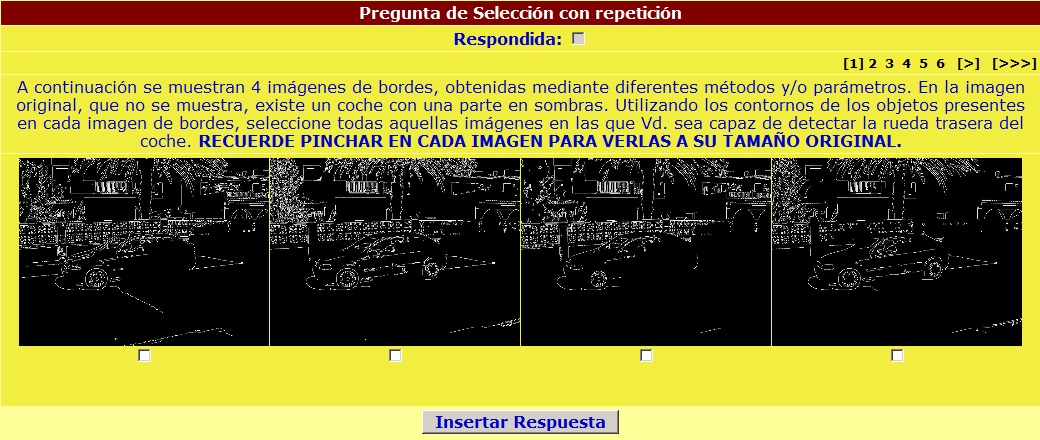
\includegraphics[width=26pc]{gfx/wemcas/wemcas-seleccion-repeticion.jpg}\caption[Pregunta de \textsc{selecci�n con repetici�n}]{Pregunta de \textsc{selecci�n con repetici�n}.\label{fig:wemcas-seleccion-repeticion}}
\end{SCfigure}

\noindent Este tipo de preguntas tienen asociadas a cada \emph{imagen respuesta} un cuadro de verificaci�n, que admite que varios de ellos se encuentren activados simult�neamente.

\subsection{Preguntas de \textsc{mapeado espacial y temporal}}
Finalmente, en la Fig. \ref{fig:wemcas-mapping} se muestra un ejemplo de pregunta con \textsc{mapeo espacial y temporal} de la respuesta para una encuesta de pilotaje para la evaluaci�n de bordes.
\begin{SCfigure}[][!h]
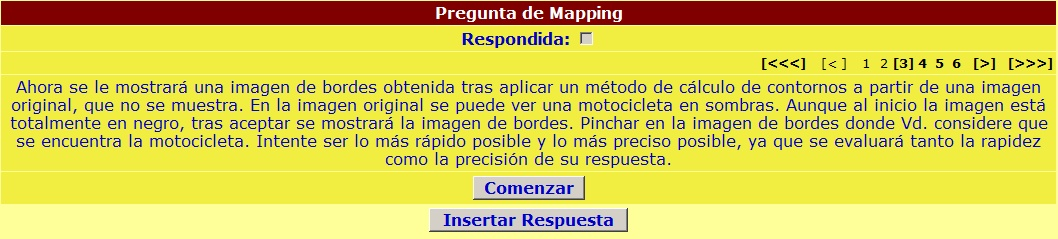
\includegraphics[width=26pc]{gfx/wemcas/wemcas-mapping.jpg}\caption[Pregunta de \textsc{Mapping}]{Pregunta de \textsc{Mapping}.\label{fig:wemcas-mapping}}
\end{SCfigure}

\noindent En este tipo de pregunta se presentan 2 ventanas, la primera, mostrada en la Fig. \ref{fig:wemcas-mapping}, con el texto de la pregunta y un bot�n \emph{Comenzar}, que al pulsarlo muestra la imagen de bordes que se pretende evaluar. Al contemplarse en este tipo de preguntas el tiempo de respuesta, la carga de la imagen se realiza en segundo plano mientras que se muestra el texto de la pregunta. Al pulsar el bot�n de comienzo, se inicia el contador de tiempo y se muestra la imagen precargada en una ventana externa (por lo que para un correcto funcionamiento del sistema hay que desactivar cualquier tipo de software bloqueador de \emph{pop--up}). En dicha ventana, se muestra la imagen y se espera a que el usuario clique con el rat�n en alg�n sitio de la ventana, momento en el que el contador de tiempos se para y se pregunta si se desea almacenar la posici�n marcada como respuesta. En caso afirmativo, se almacena en el sistema tanto el tiempo empleado en cliquear como la posici�n $(x,y)$ de dicha respuesta.
\clearpage
\section{Conclusiones}
\lettrine{E}{n} este cap�tulo se ha analizado el llamado \emph{sesgo por finalidad}, que ha sido identificado como una fuente de distorsi�n en las respuestas de los encuestados y que no se tiene conocimiento de que hubiera sido descrito previamente. Tambi�n, se han propuesto algunas recomendaciones de dise�o de cuestionarios que incorporen elementos visuales dentro de las opciones de respuesta. Estas recomendaciones se han obtenido mediante experimentaci�n y metaencuestas sobre entrevistados que cumplimentaron encuestas de pilotaje. Se ha propuesto un conjunto de tipos de preguntas que facilitan el dise�o correcto de este tipo de cuestionarios. Hay que hacer especial hincapi� en las preguntas con respuestas de \textsc{mapeado espacial y temporal}, ya que son una aportaci�n muy importante que hace esta Tesis para el desarrollo de cuestionarios para evaluaci�n de im�genes.\\
\noindent A pesar de que estas recomendaciones son, en muchos casos de sentido com�n, ser�a conveniente realizar un estudio estad�stico m�s pormenorizado que corroborase cient�ficamente las afirmaciones que se han realizado en este cap�tulo. Este estudio no se ha realizado porque exced�a los l�mites de la presente Tesis, pero desde luego abre un interesante campo de trabajo para futuras investigaciones y tesis doctorales.\\
\noindent Tambi�n es de sumo inter�s, y es otra de las aportaciones importantes de esta Tesis Doctoral, la construcci�n de un sistema Web para la construcci�n de cuestionarios con contenidos multimedia por parte de los encuestadores, y para el manejo y relleno de dichas encuestas por parte de los encuestados.\\
\subsection{Conclusiones de la Parte \textsc{\ref{part:metodoYmateriales}}}
\noindent Con este cap�tulo se finaliza la Parte \textsc{\ref{part:metodoYmateriales}}, \emph{M�todo y Materiales}, en la que se han descrito las aportaciones cient�ficas m�s relevantes de esta Tesis Doctoral. A lo largo del Cap�tulo \ref{chap:convLIP} se describi� matem�ticamente el nuevo operador \emph{Convoluci�n--\textsc{LIP}}, exponi�ndose adem�s dos implementaciones diferentes del mismo, \textsc{DGLIP--Conv} y \textsc{FGLIP--Conv}. En el Cap�tulo \ref{chap:criterios} se especificaron los criterios generales y espec�ficos que se han seleccionado para este trabajo y que han condicionado en gran medida las decisiones de investigaci�n tomadas. Para evaluar los resultados de los algoritmos de extracci�n de bordes dise�ados bajo el modelo \person{LIP} utilizando el operador \emph{Convoluci�n--\textsc{LIP}}, en el Cap�tulo \ref{chap:recCuestCalidadBordes} se han presentado un conjunto de recomendaciones para el dise�o de cuestionarios de evaluaci�n de calidad de bordes. Tambi�n se ha presentado una herramienta Web que ha sido dise�ada expresamente para el dise�o y evaluaci�n de los cuestionarios con contenidos multimedia. El compendio de cap�tulos que forman la Parte \textsc{\ref{part:metodoYmateriales}} es el n�cleo central de esta Tesis Doctoral, ya que en estos cap�tulos se han expuesto las innovaciones cient�ficas. La siguiente Parte \textsc{\ref{part:resultadosExperimentales}}, \emph{Resultados Experimentales}, comenzar� con un cap�tulo en el que se presentar�n experimentos y aplicaciones del nuevo operador propuesto \emph{Convoluci�n--\textsc{LIP}}, comparando los tiempos de computaci�n entre diferentes implementaciones. Tras ese cap�tulo, se mostrar�n los resultados obtenidos a partir del cuestionario de evaluaci�n de im�genes de bordes, tanto para pacientes con \textsc{Baja Visi�n} como para pacientes con un grado de \textsc{Visi�n Est�ndar}.
%-----------------------------
\myPart{Resultados Experimentales}\label{part:resultadosExperimentales}
\myChapter{Aplicaciones Convoluci�n LIP}\label{chap:aplicacionesConvLIP}
\minitoc\mtcskip
\vfill
\lettrine{P}{ara} mostrar la aplicabilidad de la \mbox{\emph{Convoluci�n--\textsc{LIP}}} se mostrar�n una serie de experimentos con diversas t�cnicas habituales y bien conocidas en la literatura cient�fica tradicional, adaptadas al paradigma \textsc{LIP}. Se han realizado experimentos con algoritmos de extracci�n de bordes y otros algoritmos de filtrado paso baja. Se han realizado experimentos con todos los algoritmos seleccionados en el Cap. \ref{chap:criterios}. Se comienza con un algoritmo ya implementado en \textsc{LIP}, el m�todo \emph{LIP--Sobel}. �ste muestra que se obtienen los mismos resultados implementando el algoritmo con el m�todo original y utilizando el mecanismo de \mbox{\emph{Convoluci�n--\textsc{LIP}}}, implementada �sta mediante cualquiera de las dos versiones (\mbox{\textsc{DGLIP--Conv}} o \mbox{\textsc{FGLIP--Conv}}). Tras este primer experimento, se realizan experimentos con filtros de emborronamiento para la reducci�n del ruido, basados en un filtrado \emph{media} y en un filtrado gaussiano. Se continuar� con experimentos con filtros de extracci�n de bordes, el \emph{Laplaciano de Gaussianas} y el m�todo de \emph{Canny}. Para finalizar el cap�tulo se muestran las comparativas de tiempos de c�mputo y las ganancias de velocidad, en las que se puede ver que \mbox{\textsc{FGLIP--Conv}} es la implementaci�n m�s r�pida para todos los algoritmos que se dise�en bajo el modelo \textsc{LIP}. 
\clearpage
\section{LIP--Sobel}\label{sec:lipSobel}
\lettrine{I}{nicialmente}, se va a mostrar que los algoritmos dise�ados utilizando cualquiera de las dos implementaciones del operador \emph{Convoluci�n--\textsc{LIP}} (\mbox{\textsc{DGLIP--Conv}} o \mbox{\textsc{FGLIP--Conv}}), definidas en el Cap. \ref{chap:convLIP},  producen el mismo resultado que los algoritmos previamente dise�ados por otros autores siguiendo la metodolog�a \textsc{LIP}. Para ello, la comparaci�n se realizar� con un m�todo llamado \emph{LIP--Sobel}, propuesto inicialmente por \person{Deng y Pinoli} \citep{deng98}. Este m�todo es la reformulaci�n del m�todo de extracci�n de bordes de \emph{Sobel} siguiendo el modelo \textsc{LIP}. Los autores dise�aron unas f�rmulas adaptadas a \textsc{LIP}, mediante un proceso totalmente \mbox{\emph{off--line}}, a partir de los filtros habituales de \emph{Sobel}, ya que los valores de los filtros que iban a aplicar eran constantes conocidas y fijadas previamente. Estas f�rmulas dise�adas son espec�ficas para este proceso en particular y no puede exportarse a otras aplicaciones o algoritmos, por lo tanto se puede afirmar que no es un proceso general, sino espec�fico para ese m�todo. Sin embargo, es f�cilmente deducible que la metodolog�a s� es generalizable a otros filtros, siempre y cuando los valores de dichos filtros sean constantes y conocidos \apriori.
\subsection{Formulaci�n}
Ya que el filtro de \emph{convoluci�n} es suficientemente peque�o se puede asumir que la \emph{iluminaci�n} dentro de un �rea tan reducida es constante. Esto ha producido un m�todo que se comporta de manera casi invariante ante los cambios de iluminaci�n y proporciona una respuesta mucho m�s satisfactoria para la detecci�n de los contornos de objetos en sombras que el m�todo \emph{Sobel} original (es decir, sin \textsc{LIP}). Este nuevo m�todo detecta bordes tanto en zonas bien iluminadas como en las pobremente iluminadas o en las sobreiluminadas.\\
\noindent Sea un �rea o un entorno de \emph{tonos de gris}, definida por:
\begin{equation}
\begin{array}{ccc}
\widehat{f_1}&\widehat{f_2}&\widehat{f_3}\\
\widehat{f_4}&\circledtwochars{\widehat{f_5}}&\widehat{f_6}\\
\widehat{f_7}&\widehat{f_8}&\widehat{f_9}\\
\end{array}
\label{eq:vecindario3x3}\end{equation}
\noindent donde $\widehat{f_5}$ es el p�xel central del entorno que se est� considerando.\\
\noindent Utilizando \eqref{eq:mascarasSobelSTD}, en la p�g. \pageref{eq:mascarasSobelSTD}, que muestra las m�scaras originales del m�todo de \emph{Sobel}, y siguiendo el m�todo directo de \textsc{LIP}, se ha definido el \emph{\textsc{vector}} de \emph{tonos de gris} del m�todo de \mbox{\emph{LIP--Sobel}}, $\vec{g}=(g_x,g_y)$, como:
\begin{eqnarray}
g_x = &\left(\widehat{f_1}\LIPplus \left(2\LIPtimes \widehat{f_4}\right) \LIPplus \widehat{f_7}\right)\LIPminus \left(\widehat{f_3}\LIPplus \left(2\LIPtimes \widehat{f_6}\right) \LIPplus \widehat{f_9}\right)\quad &\\
g_y = &\left(\widehat{f_1}\LIPplus \left(2\LIPtimes \widehat{f_2}\right) \LIPplus \widehat{f_3}\right)\LIPminus \left(\widehat{f_7}\LIPplus \left(2\LIPtimes \widehat{f_8}\right) \LIPplus \widehat{f_9}\right)\quad &
\end{eqnarray}
\noindent Los autores pudieron definir las f�rmulas que generan el vector del m�todo \mbox{\emph{LIP--Sobel}} porque se conocen los valores del filtro previamente y adem�s, son constantes (valores positivos y negativos, que se tradujeron a la formulaci�n directa de \textsc{LIP} mediante $\LIPplus$ � $\LIPminus$, respectivamente). Utilizando la funci�n isom�rfica de transformaci�n, $\varphi(\cdot)$, descrita en \eqref{eq:isomorTransf}, se obtiene (ver demostraci�n en \citep[Ap�ndice 3]{deng98}):
\begin{eqnarray}
g_x = M-M\left(\frac{f_3 f_6^2 f_9}{f_1 f_4^2 f_7}\right)\label{eq:lipSobelGX}\\
g_y = M-M\left(\frac{f_1 f_2^2 f_3}{f_7 f_8^2 f_9}\right)\label{eq:lipSobelGY}
\end{eqnarray}
\noindent Se deduce f�cilmente que \eqref{eq:lipSobelGX} y \eqref{eq:lipSobelGY} se pueden obtener directamente de la formulaci�n de \mbox{\textsc{DGLIP--Conv}}, mostrada en \eqref{eq:prodLIPgt}, p�g. \pageref{eq:prodLIPgt}, utilizando las m�scaras definidas en \eqref{eq:mascarasSobelSTD}. Por tanto, \mbox{\textsc{DGLIP--Conv}} es una formulaci�n m�s general que el m�todo planteado por \person{Deng y Pinoli}, y consecuentemente, al ser equivalentes las dos formulaciones, \mbox{\textsc{FGLIP--Conv}}, tambi�n es una formulaci�n m�s general que la propuesta por \person{Deng y Pinoli}.
\subsection{Resultados experimentales}
Aunque en el Cap. \ref{chap:criterios} se han seleccionado una serie de im�genes, para comprobar el correcto funcionamiento del m�todo \emph{LIP--Sobel} en sus diferentes implementaciones y facilitar la comparaci�n visual, se ha decidido utilizar alguna imagen conocida y habitual en las comparaciones del �mbito del \textsc{Procesamiento de Im�genes}. Para ello, se ha seleccionado la conocida imagen \texttt{peppers} (ver Fig. \ref{fig:originalPeppers}).%\clearpage
\begin{SCfigure}[][!t]
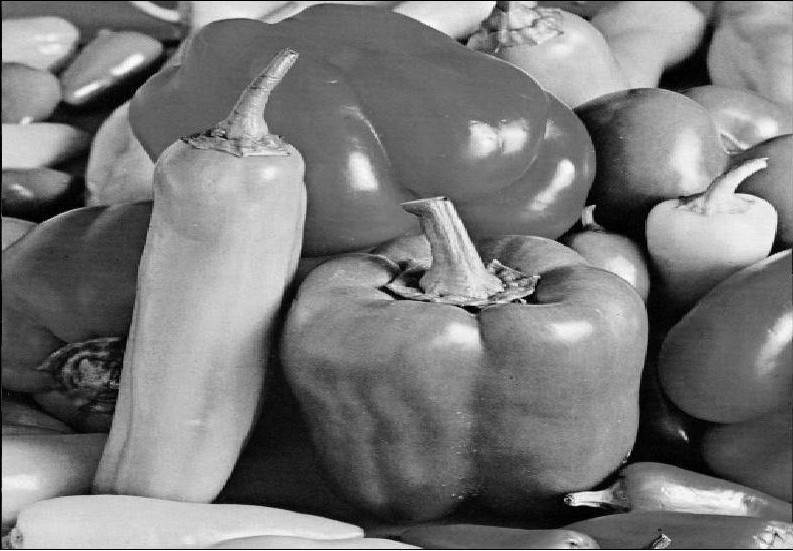
\includegraphics[width=21pc]{gfx/originalPeppers}\caption[Imagen Original]{Imagen \texttt{peppers} original.\label{fig:originalPeppers}}
\end{SCfigure}

\noindent La Fig. \ref{fig:darkenedPeppers} muestra la imagen resultante tras aplicar un proceso de oscurecimiento no lineal sobre la imagen original (Fig. \ref{fig:originalPeppers}). El proceso de oscurecimiento se ha realizado con la f�rmula:
\begin{equation}
\mathrm{dark}(x,y) = \mathrm{img}(x,y)\cdot\left(0.1 + \frac{5\cdot\sin(2\pi x)}{6\cdot \mathrm{width}}\right).\label{eq:darkening}
\end{equation}
\noindent Donde ``$\mathrm{width}$'' es la anchura de la imagen que se desea oscurecer e $\mathrm{img}(x,y)$ es el valor del p�xel $(x,y)$ de dicha imagen original.
\begin{SCfigure}[][!t]
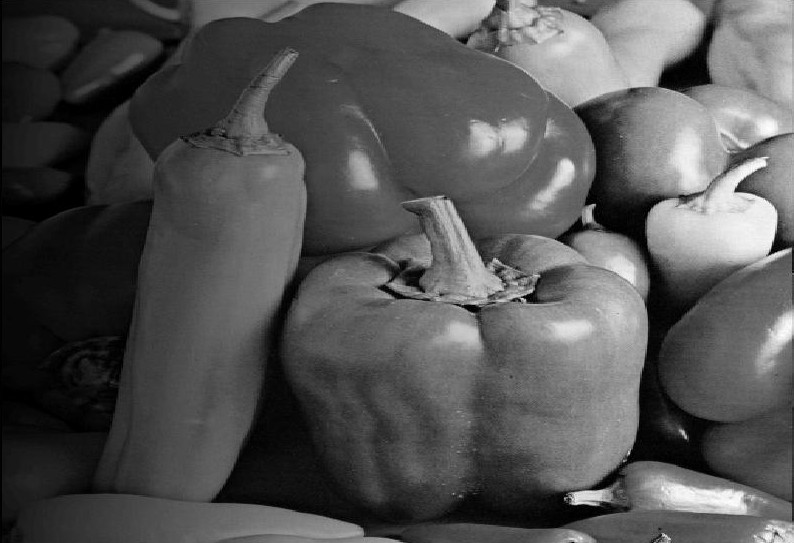
\includegraphics[width=21pc]{gfx/darkenedPeppers}\caption[Imagen Oscurecida]{Imagen \texttt{peppers} oscurecida.}\label{fig:darkenedPeppers}
\end{SCfigure}
\begin{SCfigure}[][!t]
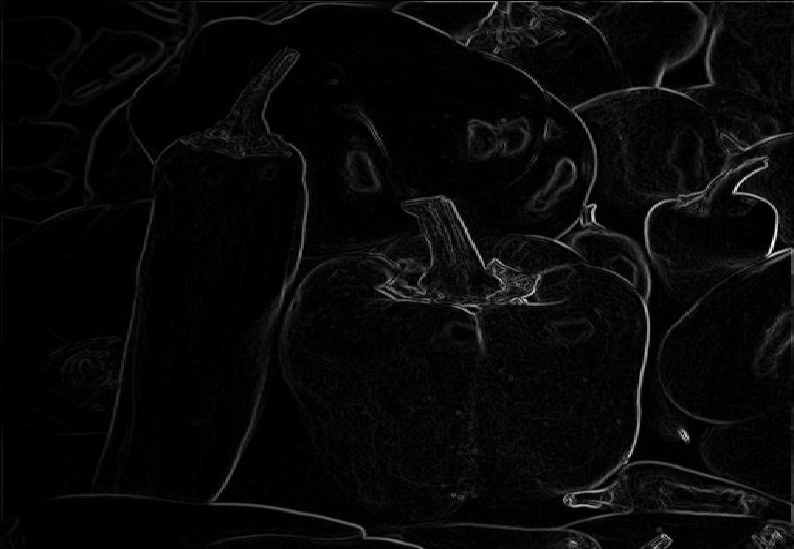
\includegraphics[width=21pc]{gfx/peppersSobel}\caption[Imagen Sobel]{Sobel est�ndar aplicado sobre la imagen \texttt{peppers} oscurecida.\label{fig:stdsobel}}
\end{SCfigure}
\begin{SCfigure}[][!t]
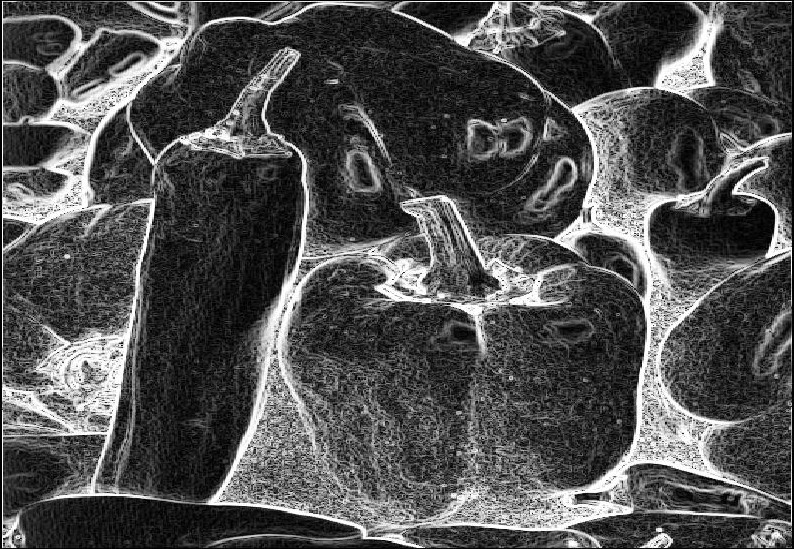
\includegraphics[width=21pc]{gfx/peppersSobelLIPDengPinoli}\caption[Imagen LIP--Sobel]{LIP--Sobel aplicado sobre la imagen \texttt{peppers} oscurecida.\label{fig:lipsobel}}
\end{SCfigure}

\noindent A continuaci�n, se muestran los resultados de \emph{LIP--Sobel} construidos con tres metodolog�as diferentes (siguiendo el m�todo propuesto por \person{Deng y Pinoli} \citep{deng98}, mediante \mbox{\textsc{DGLIP--Conv}} y mediante \mbox{\textsc{FGLIP--Conv}}). Como era de esperar, los resultados obtenidos por los tres m�todos son exactamente iguales, como demuestra que el \definicion[-2em]{\textsc{MSE}}{Del ingl�s, \textsc{Mean Squared Error}, Error cuadr�tico medio.} sea cero en todos los casos.
\subsubsection{LIP--Sobel implementado mediante el procedimiento de \person{Deng y Pinoli}}
En la Fig. \ref{fig:stdsobel} se muestra la imagen resultante de aplicar el m�todo \emph{Sobel} est�ndar sobre la imagen oscurecida (Fig. \ref{fig:darkenedPeppers}). Se ha aplicado sobre la Fig. \ref{fig:darkenedPeppers} el m�todo \emph{LIP--Sobel} tal y como fue propuesto por \person{Deng y Pinoli}, descrito en \eqref{eq:lipSobelGX} y \eqref{eq:lipSobelGY}. En la Fig. \ref{fig:lipsobel} se muestra la magnitud del gradiente de la imagen resultante. Como se puede observar en la imagen de la Fig. \ref{fig:stdsobel}, que muestra la aplicaci�n del m�todo \emph{Sobel} original, los bordes presentes en las regiones oscuras de la imagen original no se han detectado con claridad. Frente a esta imagen, se puede observar la Fig. \ref{fig:lipsobel}, donde se muestra el resultado del m�todo \emph{LIP--Sobel}, en la que los bordes en las regiones oscuras se detectan de manera m�s homog�nea. Este comportamiento es un beneficio colateral, debido a que \textsc{LIP} hace que la componente de \emph{iluminaci�n} se pueda considerar constante en un entorno peque�o. Gracias al comportamiento logar�tmico de \textsc{LIP}, dicha componente se elimina autom�ticamente al realizar la operaci�n \emph{Convoluci�n--\textsc{LIP}} con un filtro cuya suma de componentes sea nula, o bien, al realizar operaciones $\LIPplus$ y $\LIPminus$ que se compensen entre s�.
\subsubsection{LIP--Sobel implementado mediante \mbox{\textsc{FGLIP--Conv}} y \mbox{\textsc{DGLIP--Conv}}}

\noindent El filtro \emph{Sobel} est�ndar, mostrado en \eqref{eq:mascarasSobelSTD}, es un filtro separable, compuesto por dos vectores:
\begin{eqnarray}
\vec{a}&=&[-1,0,1]\nonumber\\
\vec{b}&=&[1,2,1]\label{eq:separableSobelMask}
\end{eqnarray}

\noindent Usando la propiedad de separabilidad de los filtros de \emph{Sobel}, se puede usar el operador \emph{Convoluci�n--LIP}, implementado tanto por el m�todo \mbox{\textsc{DGLIP--Conv}} como por el m�todo \mbox{\textsc{FGLIP--Conv}}. De modo que para realizar el algoritmo \emph{LIP--Sobel} mediante el m�todo \mbox{\textsc{DGLIP--Conv}}, se aplica \eqref{eq:prodLIPgt} utilizando $\vec{a}$ y $\vec{b}$ tal y como se ha propuesto en \eqref{eq:separableSobelMask} a la imagen oscurecida (Fig. \ref{fig:darkenedPeppers}). De manera an�loga, se obtiene el mismo resultado utilizando el algoritmo \emph{LIP--Sobel} mediante el mecanismo \mbox{\textsc{FGLIP--Conv}}, para lo que se aplicar� \eqref{eq:convLIPgt} con $\vec{a}$ y $\vec{b}$, descritos en \eqref{eq:separableSobelMask}. Los bordes detectados por \emph{LIP--Sobel} mediante cualquiera de los tres procedimientos (\person{Deng y Pinoli}, \mbox{\textsc{DGLIP--Conv}} y \mbox{\textsc{FGLIP--Conv}}) son los mismos y, como se ha comentado con anterioridad, el \textsc{MSE} es cero.
%\clearpage
\section{Filtros de emborronamiento}
\lettrine{E}{n} la aplicaci�n previa se ha mostrado que los dos mecanismos propuestos para el desarrollo del operador \emph{Convoluci�n--LIP} proporcionan los mismos resultados para un algoritmo en particular mediante el uso de un algoritmo dise�ado espec�ficamente. Sin embargo, el nuevo operador \emph{Convoluci�n--LIP} es m�s interesante y vers�til, y a continuaci�n, se mostrar�n experimentos que van a permitir refrendar esta afirmaci�n.\\
\noindent Siguiendo el mismo procedimiento que utilizaron \person{Deng y Pinoli} para obtener la formulaci�n con la que se implement� el m�todo \emph{LIP--Sobel} original, se podr�a dise�ar cualquier otro filtro. Sin embargo, cada filtro deber�a calcularse de manera expl�cita previamente; por ejemplo, aunque s�mplemente se desease modificar el tama�o del filtro para que tenga un entorno diferente, se deber�a calcular un filtro completamente nuevo, sin poder adaptarse el calculado previamente. Justo al contrario, el operador \emph{Convoluci�n--LIP}, ya sea implementado mediante \mbox{\textsc{DGLIP--Conv}} o mediante \mbox{\textsc{FGLIP--Conv}}, permite utilizar el mismo c�digo, simplemente cambiando los par�metros de entrada (los filtros 1D utilizados), lo cual se traduce en una ganancia en flexibilidad y, a su vez, en robustez de las aplicaciones. Adem�s de estas ventajas, se obtiene una mejora en el tiempo de desarrollo y sobre todo en el tiempo de c�mputo, como se mostrar� en la Sec. \ref{sec:tiemposComputo}.
\subsection{Filtro Media: LIP--Avg}
En este apartado, se va a mostrar el que se puede considerar como ``mejor caso'' en t�rminos de velocidad para el mecanismo de construcci�n de filtros siguiendo la filosof�a \textsc{LIP} desarrollada por \person{Deng y Pinoli}. Para ello, sea un filtro en el que todos los elementos son constantes y con valores id�nticos, por ejemplo, un filtro \emph{media}. Se afirma que �ste es el ``mejor caso'' para el mecanismo de \person{Deng y Pinoli}, ya que la potenciaci�n, que es una operaci�n computacionalmente muy costosa, se puede realizar solo una �nica vez por filtro, tal y como se demuestra a continuaci�n. Se compara este resultado con las im�genes resultantes obtenidas mediante \mbox{\textsc{DGLIP--Conv}} y mediante \mbox{\textsc{FGLIP--Conv}}, comprob�ndose que el resultado es el mismo, pero el tiempo de ejecuci�n de estos �ltimos es menor que el ``mejor caso'' del mecanismo propuesto por \person{Deng y Pinoli}.
\subsubsection{LIP--Avg implementado mediante el procedimiento de \person{Deng y Pinoli}}
Se define un filtro de tama�o $n\times n$ p�xeles para que calcule la media de dicho entorno siguiendo el paradigma \textsc{LIP}.  Como primer paso, se fija el valor de $n$, para poder construir la f�rmula espec�fica asociada al filtro \emph{media}. Por ejemplo, si se toma $n = 3$, se puede utilizar la misma definici�n de entorno de un p�xel que en \eqref{eq:vecindario3x3}, con lo que se obtiene:
\begin{eqnarray}
\mathrm{avg^{3\times 3}_{LIP}}(f)=\Big( &\left(\frac{1}{9} \LIPtimes \widehat{f_1}\right)\LIPplus \left(\frac{1}{9} \LIPtimes \widehat{f_2}\right)\LIPplus \left(\frac{1}{9} \LIPtimes \widehat{f_3}\right)& \LIPplus \nonumber \\
&\left(\frac{1}{9} \LIPtimes \widehat{f_4}\right)\LIPplus \left(\frac{1}{9} \LIPtimes \widehat{f_5}\right)\LIPplus \left(\frac{1}{9} \LIPtimes \widehat{f_6}\right)& \LIPplus \nonumber \\
&\left(\frac{1}{9} \LIPtimes \widehat{f_7}\right)\LIPplus \left(\frac{1}{9} \LIPtimes \widehat{f_8}\right)\LIPplus \left(\frac{1}{9} \LIPtimes \widehat{f_9}\right)\Big)&
\end{eqnarray}
\noindent Operando sobre esta f�rmula, se obtiene:
\begin{equation}
\mathrm{avg^{3\times 3}_{LIP}}(f)= M - \left(f_1 \cdot f_2 \cdot f_3 \cdot f_4 \cdot f_5 \cdot f_6 \cdot f_7 \cdot f_8 \cdot f_9 \right)^{\frac{1}{9}}\\
\end{equation}
\noindent Que se podr�a abreviar como,
\begin{equation}
\mathrm{avg^{3\times 3}_{LIP}}(f)= M - \left(\prod^{9}_{i=1} f_i \right)^{\frac{1}{9}}
\end{equation}
\noindent Hay que notar que se puede tomar un exponente com�n $\left(\frac{1}{9}\right)$. Al utilizarlo, el tiempo de ejecuci�n puede disminuir, ya que se reduce sensiblemente la complejidad de la f�rmula que se ha de codificar.\\
\noindent Tambi�n se ha probado con un entorno de mayor tama�o: $5 \times 5$. Para este caso, la nueva f�rmula obtenida es:
\begin{equation}
\mathrm{avg^{5\times 5}_{LIP}}(f)= M - \left(\prod^{25}_{i=1} f_i \right)^{\frac{1}{25}}
\end{equation}
\noindent Est� claro que para cada valor diferente de $n$, es decir, para cada tama�o del entorno que se considere, se tiene que calcular una nueva f�rmula. Por lo tanto, es necesario reescribir nuevo c�digo para cada nuevo tama�o del filtro.
\subsubsection{LIP--Avg implementado mediante \mbox{\textsc{DGLIP--Conv}} y \mbox{\textsc{FGLIP--Conv}}}
Mediante el operador \emph{Convoluci�n--LIP} se puede construir f�cilmente el filtro media siguiendo la metodolog�a \textsc{LIP} para entornos de cualquier tama�o. Para implementar \emph{LIP--Avg} de $3\times 3$ p�xeles, s�lo se tiene que aplicar \eqref{eq:prodLIPgt} � \eqref{eq:convLIPgt}, dependiendo de si la implementaci�n es siguiendo el m�todo \mbox{\textsc{DGLIP--Conv}} o \mbox{\textsc{FGLIP--Conv}} respectivamente, y utilizando como componentes del filtro los vectores $\vec{a} = \vec{b} =  \left[\frac{1}{3},\frac{1}{3},\frac{1}{3}\right]$.\\
\noindent Para calcular \emph{LIP--Avg} de $5\times 5$, se utiliza \eqref{eq:prodLIPgt} � \eqref{eq:convLIPgt} con los vectores $\vec{a} = \vec{b} =  \left[\frac{1}{5},\frac{1}{5},\frac{1}{5},\frac{1}{5},\frac{1}{5} \right]$. Se puede deducir f�cilmente que, simplemente, cambiando los filtros que se utilizan como par�metros de entrada, se puede obtener el c�lculo de cualquier filtro \emph{media} para diferentes tama�os del entorno, sin necesidad de escribir una sola l�nea de c�digo adicional.
\subsection{Filtro Gaussiano: LIP--GBlur}
En el apartado anterior, se han mostrado un par de ejemplos de lo que se puede considerar el caso m�s favorable para la metodolog�a propuesta por \person{Deng y Pinoli}. Este ``mejor caso'' se debe a la reducci�n del n�mero de exponenciaciones utilizadas, ya que cada p�xel del entorno se eleva al mismo valor, y por tanto, se puede tomar un exponente com�n. Por tanto, el ``peor caso'' para la metodolog�a de \person{Deng y Pinoli} es un filtro con valores  diferentes, en el que no se pudiera optimizar sacando un exponente com�n. Un ejemplo de este tipo es el de emborronamiento gaussiano, donde el filtro est� generado por una gaussiana. Se ha escogido un filtro gaussiano bidimensional puesto que es separable: la manera habitual de calcular un filtro gaussiano bidimensional es mediante la multiplicaci�n matricial de un filtro gaussiano unidimensinal (vector columna) por s� mismo traspuesto (vector fila). Para mostrar un ejemplo espec�fico, se ha generado un filtro gaussiano de tama�o $7\times 7$ (ver Tab. \ref{tbl:gauss2d}), realizado mediante la aproximaci�n de una gaussiana (con $\sigma = 1.0$) para una malla de $7\times 7$ p�xeles.\\
\noindent A continuaci�n, se muestran los resultados obtenidos por el filtro \emph{LIP--GBlur}, que muestra el emborronamiento gaussiano siguiendo la filosof�a \textsc{LIP}, mediante los tres m�todos indicados anteriormente. Como era de esperar, no se han obtenido diferencias entre los resultados obtenidos por los diferentes m�todos para la implementaci�n del mismo filtro.
\subsubsection{LIP--GBlur implementado mediante el procedimiento de \person{Deng y Pinoli}}
Se ha extendido la definici�n del entorno de p�xeles en el mismo sentido de \eqref{eq:vecindario3x3} a un entorno de $7\times 7$ p�xeles. El filtro gaussiano utilizado se detalla en la \mbox{Tab. \ref{tbl:gauss2d}}.
\begin{SCtable}[][!t]
  \begin{tabular}{|ccccccc|}
      \hline
      \small 0.0001 & \small 0.0015 & \small 0.0067 & \small 0.0111 & \small 0.0067 & \small 0.0015 & \small 0.0001\\
      \small 0.0015 & \small 0.0183 & \small 0.0821 & \small 0.1353 & \small 0.0821 & \small 0.0183 & \small 0.0015\\
      \small 0.0067 & \small 0.0821 & \small 0.3679 & \small 0.6065 & \small 0.3679 & \small 0.0821 & \small 0.0067\\
      \small 0.0111 & \small 0.1353 & \small 0.6065 & \small 1.0000 & \small 0.6065 & \small 0.1353 & \small 0.0111\\
      \small 0.0067 & \small 0.0821 & \small 0.3679 & \small 0.6065 & \small 0.3679 & \small 0.0821 & \small 0.0067\\
      \small 0.0015 & \small 0.0183 & \small 0.0821 & \small 0.1353 & \small 0.0821 & \small 0.0183 & \small 0.0015\\
      \small 0.0001 & \small 0.0015 & \small 0.0067 & \small 0.0111 & \small 0.0067 & \small 0.0015 & \small 0.0001\\
      \hline
  \end{tabular}\caption[Gauss $7\times 7$]{Malla de $7\times 7$ p�xeles de un filtro gaussiano bidimensional (con $\sigma = 1.0$).\label{tbl:gauss2d}}
\end{SCtable}

\noindent La f�rmula que se aplica para obtener el emborronamiento gaussiano bajo el paradigma \textsc{LIP}, \emph{LIP--GBlur}, se muestra en \eqref{eq:gaussianLIPdpOrig}, aunque por simplicidad, no se muestran todos los valores de la f�rmula.
\begin{eqnarray}
&\mathrm{GBlur_{LIP}}(f)=&\nonumber \\
\Big( &\left(\scriptstyle{0.0001}\LIPtimes\widehat{f_1}\right)\LIPplus\left(\scriptstyle{0.0015}\LIPtimes \widehat{f_2}\right)\LIPplus\left(\scriptstyle{0.0067}\LIPtimes\widehat{f_3}\right)\LIPplus &\ldots \nonumber\\
\ldots &\left(\scriptstyle{0.1353}\LIPtimes\widehat{f_{23}}\right)\LIPplus\left(\scriptstyle{0.6065}\LIPtimes \widehat{f_{24}}\right)\LIPplus\left(\scriptstyle{1.0000}\LIPtimes\widehat{f_{25}}\right)\LIPplus &\ldots \nonumber \\
\ldots & \left(\scriptstyle{0.0067}\LIPtimes\widehat{f_{47}}\right)\LIPplus\left(\scriptstyle{0.0015}\LIPtimes \widehat{f_{48}}\right)\LIPplus\left(\scriptstyle{0.0001}\LIPtimes\widehat{f_{49}}\right)&\Big)\nonumber\\
\label{eq:gaussianLIPdpOrig}
\end{eqnarray}

\noindent An�logamente a lo realizado para obtener \eqref{eq:lipSobelGX} y \eqref{eq:lipSobelGY}, se obtiene la f�rmula \eqref{eq:gaussianLIPdp}.
\begin{equation}
\mathrm{GBlur_{LIP}}(f)= M - \left(\frac{f_1^{\scriptscriptstyle{0.0001}} \cdot \ldots \cdot f_{24}^{\scriptscriptstyle{0.6065}} \cdot
 f_{25}^{\scriptscriptstyle{1.000}}\cdot\ldots\cdot f_{49}^{\scriptscriptstyle{0.0001}}}{M^{\scriptscriptstyle{0.0001
\cdot\ldots\cdot 0.6065 \cdot 1.0000 \cdot\ldots\cdot
0.0001}}}\right)\label{eq:gaussianLIPdp}
\end{equation}

\subsubsection{LIP--GBlur implementado mediante \mbox{\textsc{DGLIP--Conv}} y \mbox{\textsc{FGLIP--Conv}}}
Como se ha indicado anteriormente, la matriz bidimensional de una gaussiana es un filtro separable, construido a partir de la multiplicaci�n de un vector de una gaussiana unidimensional consigo mismo. El tama�o del filtro depende del valor del par�metro $\sigma$: cuanto mayor es $\sigma$, m�s grande debe ser el tama�o del filtro para que pueda tener suficiente precisi�n. Como regla general, la longitud del filtro gaussiano, centrado sobre una posici�n espec�fica, debe ser de $3.5\cdot\sigma^2$ valores a izquierda y derecha de dicha posici�n (est� ampliamente aceptado el redondeo hacia el valor inferior). Por ejemplo, para $\sigma = 1$, se debe tomar un filtro gaussiano de tama�o $7$. Como ejemplo, para dicho valor de $\sigma$, en los experimentos se han utilizado los siguientes vectores:
\begin{equation}
      \vec{a} = \vec{b} = \left[0.011, 0.135, 0.606, 1, 0.606, 0.135, 0.011\right]
\end{equation}

\noindent Es evidente, que para un valor m�s grande de $\sigma$, se deber� utilizar un filtro de mayor tama�o. Sin embargo, no hay necesidad alguna de reescribir ninguna l�nea de c�digo, simplemente basta con cambiar los par�metros de entrada para obtener la salida deseada. Esto es una de las mayores contribuciones de esta nueva reformulaci�n del operador \emph{convoluci�n} utilizando el paradigma \textsc{LIP}, propuesto en este trabajo.

\section{Filtros para la extracci�n de bordes}
\lettrine{C}{omo} se ha expuesto en cap�tulos anteriores, los algoritmos de extracci�n de bordes ser�n las aplicaciones principales que se van a desarrollar en esta Tesis Doctoral. Por ese motivo, en este cap�tulo se mostrar� el funcionamiento de los algoritmos de extracci�n de bordes seleccionados en el Cap. \ref{chap:criterios}. El primero de los algoritmos de extracci�n de bordes seleccionados, \emph{LIP--Sobel} ya se ha expuesto en la Sec. \ref{sec:lipSobel}. A continuaci�n, se describir�n y mostrar�n los dos restantes, \emph{LIP--LoG} y \emph{LIP--Canny}, que son la implementaci�n bajo el modelo \textsc{LIP} de los algoritmos \emph{LoG} y \emph{Canny}, descritos en el Cap. \ref{chap:ProcImagenes}.
\subsection{Laplaciano de Gaussianas: LIP--LoG}
Existen muchos m�todos para la extracci�n de bordes de una imagen digital. Como se observ� anteriormente, \emph{Sobel} es un algoritmo para la obtenci�n de los contornos. Este m�todo se basa en filtros fijos de un tama�o peque�o. Sin embargo, existen otros m�todos que tienen filtros de tama�o variable y con valores en funci�n del tama�o. Uno de estos m�todos es el llamado \emph{Laplaciano de Gaussianas}, tambi�n conocido como \emph{LoG}. Este operador es la suma de la segunda derivada parcial en cada direcci�n sobre la imagen que previamente ha sufrido un emborronamiento gaussiano, aunque estas dos operaciones se hacen simult�neamente, resultando en una mayor efectividad. El operador bidimensional \emph{LoG} se realiza mediante la \emph{convoluci�n} de una imagen con un filtro \emph{LoG} bidimensional, tal y como se muestra en \eqref{eq:LoG_2D}.
\begin{equation}
LoG(I,\sigma)=\nabla^2\left\{\convtwod{\Big(I,G_\sigma(x,y)\Big)}\right\} = \convtwod\bigg(I, \Big(\nabla^2 G_\sigma(x,y)\Big)\bigg) \label{eq:LoG_2D}
\end{equation}
\noindent donde $G_\sigma(x,y)$ simboliza la funci�n 2D gaussiana descrita en \eqref{eq:Gaussian_2D} y $\nabla^2 G(x,y)$ es la suma de las segundas derivadas parciales direccionales de $G(x,y)$ mostradas en \eqref{eq:laplaciano2}.
\begin{equation}
H(x,y) = \nabla^2 G(x,y) = \frac{\partial^2 G(x,y)}{\partial x^2} + \frac{\partial^2 G(x,y)}{\partial y^2} = \frac{x^2 +y^2-2\sigma^2}{\sigma^4}e^{-\frac{x^2+y^2}{2\sigma^2}} \label{eq:laplaciano2}
\end{equation}
\noindent El detector de bordes \emph{Laplaciano de Gaussianas} habitualmente se implementa utilizando un filtro bidimensional, como se ha indicado anteriormente; sin embargo, se ha demostrado que el filtro \emph{LoG} es separable (ver \citep{vernon91} para la demostraci�n de separabilidad del filtro \emph{LoG}) y dicha aproximaci�n es la utilizada en este trabajo, tanto para implementar el filtro original \emph{LoG} como para la versi�n \emph{LIP--LoG} mediante \mbox{\textsc{FGLIP--Conv}}. Sin embargo, para implementar \emph{LIP--LoG} utilizando la metodolog�a propuesta por \person{Deng y Pinoli} no se pueden utilizar filtros separables ya que no ha sido desarrollado as� originalmente; al contrario se ha utilizado un filtro bidimensional \emph{LoG} descrito en \eqref{eq:laplaciano2}. La formulaci�n separable del filtro \emph{LoG} se muestra en \eqref{eq:LoG_separable}:
\begin{equation}\label{eq:LoG_separable}
\begin{split}
LoG(I,\sigma)=\nabla^2\Big\{&\convtwod{\Big(I,G_\sigma\Big)}\Big\} = \convoned\bigg(\convoned\Big(I,\vec{a_\sigma}(x)\Big),\vec{g_\sigma}(y)\bigg) + \\
&\convoned\bigg(\convoned\Big(I,\vec{a_\sigma}(y)\Big),\vec{g_\sigma}(x)\bigg)
\end{split}
\end{equation}
\noindent donde $G_\sigma(x,y)$ es una funci�n gaussiana bidimensional, $\vec{g_\sigma}(t)$ representa una funci�n gaussiana unidimensional y $\vec{a_\sigma}(t)$ muestra la segunda derivada de la funci�n gaussiana unidimensional, definidas respectivamente como:
\begin{eqnarray}
G_\sigma(x,y) & = & \frac{1}{2\pi\sigma^2}e^{-\frac{x^2+y^2}{2\sigma^2}} \\ \label{eq:Gaussian_2D}
\vec{g_\sigma}(t) & = &\frac{1}{\sqrt{2\pi}\sigma}e^{-\frac{t^2}{2\sigma^2}} \\ \label{eq:Gaussian_1D}
\vec{a_\sigma}(t) & = & \frac{\partial^2 G_\sigma(t)}{\partial t^2} \label{eq:laplacianGaussian_1D}
\end{eqnarray}
\noindent El tama�o del filtro de \emph{Sobel} es de $3\times 3$, sin embargo, para poder utilizar un filtro \emph{LoG} se necesita un filtro con un tama�o mayor, para este caso en particular se utiliza un filtro \emph{LoG} de $7\times 7$ p�xeles. Es decir, que se tienen $49$ elementos, cada uno con un valor diferente calculado a partir de la f�rmula \emph{LoG} descrita en \eqref{eq:Gaussian_2D}. Esto est� en relaci�n directa con el tama�o del filtro gaussiano y, obviamente, con las derivadas parciales de segundo orden del mismo.\\
\noindent Aunque \person{Deng y Pinoli} no establecieron expl�citamente un filtro \mbox{\emph{LIP--LoG}}, es f�cil extender el mecanismo que los autores utilizaron al definir la versi�n original del \emph{LIP--Sobel} para obtener un mecanismo an�logo y obtener un filtro \emph{LIP--LoG}, cuya f�rmula viene dada por:
\begin{equation}
LoG_{\upDelta}^{7\times 7}(\widehat{f}) = \LIPsum{i=1}{7}\ \ \LIPsum{j=1}{7} \left(H(i,j)\LIPtimes\widehat{f}(i,j)\right)
\end{equation}
\noindent que se traduce a la siguiente f�rmula:
\begin{equation}
LoG_{\upDelta}^{7\times 7}(\widehat{f}) = \prod_{i=1}^{7}\prod_{j=1}^{7}\left(f(i,j)^{H(i,j)}\right),\label{eq:LoG_DP}
\end{equation}
\noindent donde $H(i,j)$ es el filtro \emph{LoG} bidimensional definido en \eqref{eq:laplaciano2} y $f(i,j)$ son cada uno de los $49$ \emph{tonos de gris} diferentes de la imagen de cada \emph{convoluci�n}.\\
\begin{SCfigure}[][!t]
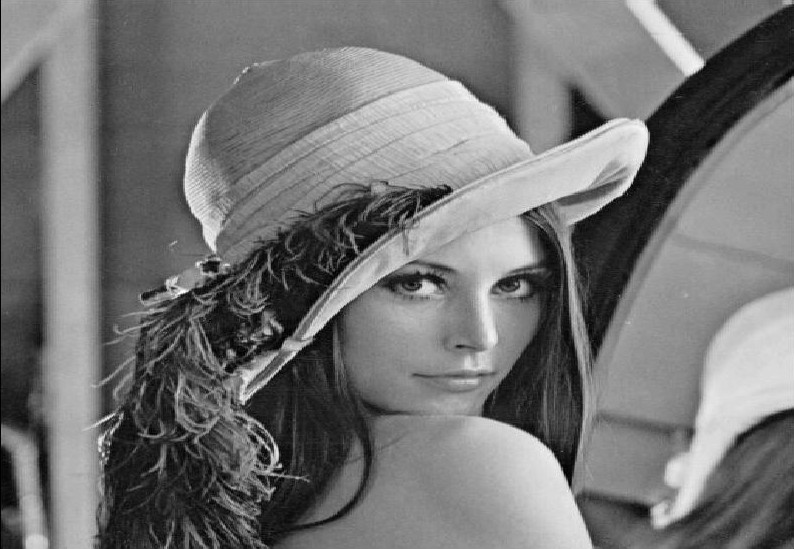
\includegraphics[width=21pc]{gfx/originalLenna}\caption[\texttt{Lenna} Original]{Imagen \texttt{Lenna} original.\label{fig:lennaOriginal}}
\end{SCfigure}
\begin{SCfigure}[][!t]
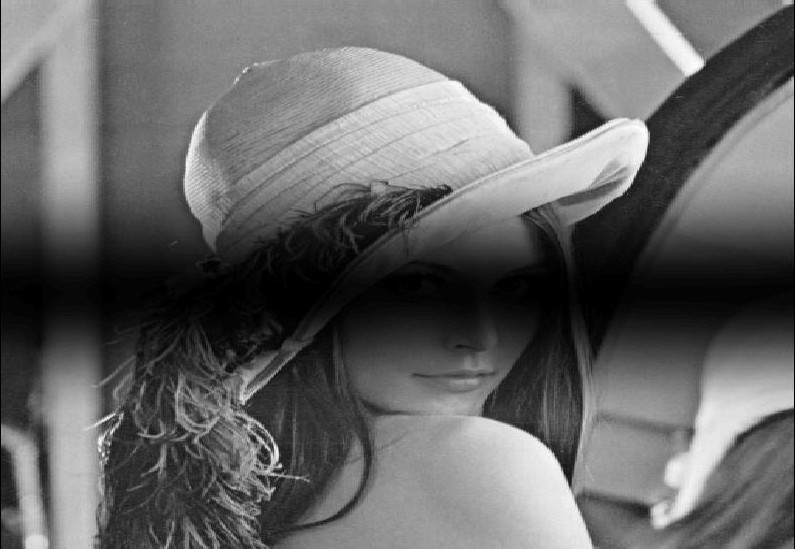
\includegraphics[width=21pc]{gfx/darkenedLenna}\caption[\texttt{Lenna} Oscurecida]{Imagen \texttt{Lenna} oscurecida.\label{fig:lennaOscurecida}}
\end{SCfigure}
\begin{SCfigure}[][!t]
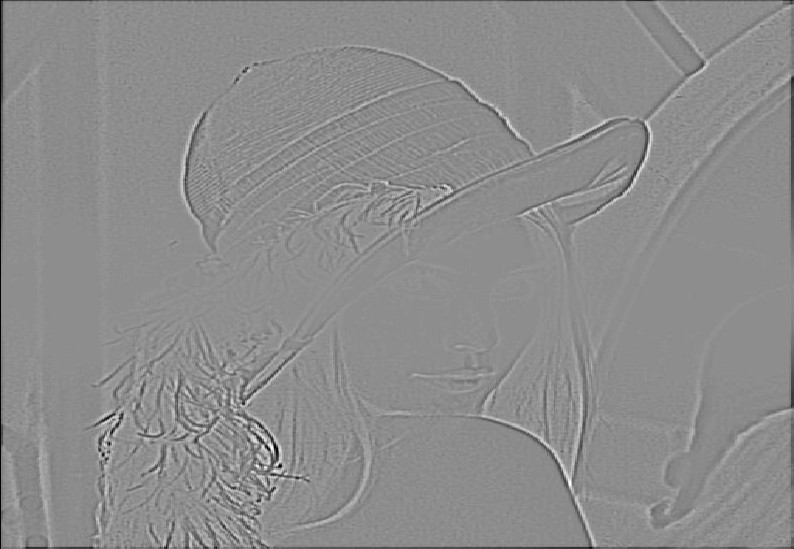
\includegraphics[width=21pc]{gfx/darkenedLennaLoG}\caption[LoG \texttt{Lenna} Oscurecida]{LoG sobre la imagen \texttt{Lenna} oscurecida.\label{fig:LoGlennaOscurecida}}
\end{SCfigure}
\begin{SCfigure}[][!t]
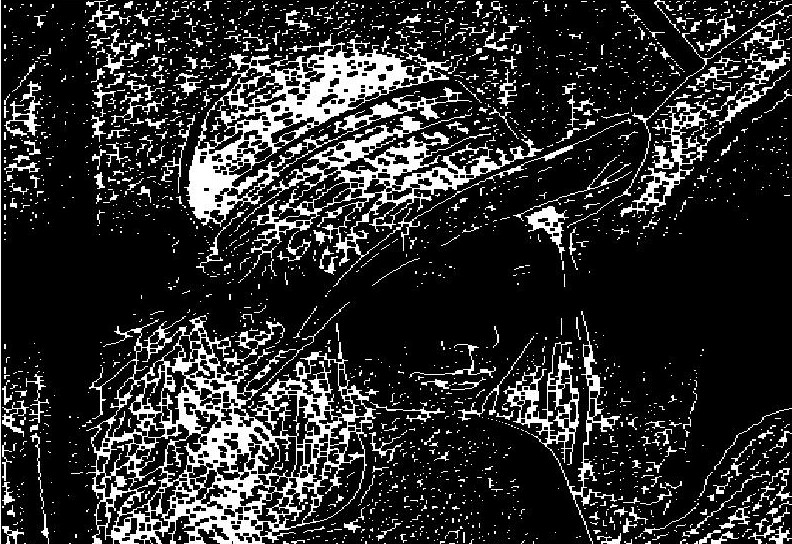
\includegraphics[width=21pc]{gfx/thresh10b_darkenedLennaLoG}\caption[LoG umbralizado \texttt{Lenna} Oscurecida]{LoG umbralizado (con $umbral = 10$) sobre la imagen \texttt{Lenna} oscurecida.\label{fig:threshLoGlennaOscurecida}}
\end{SCfigure}
\begin{SCfigure}[][!t]
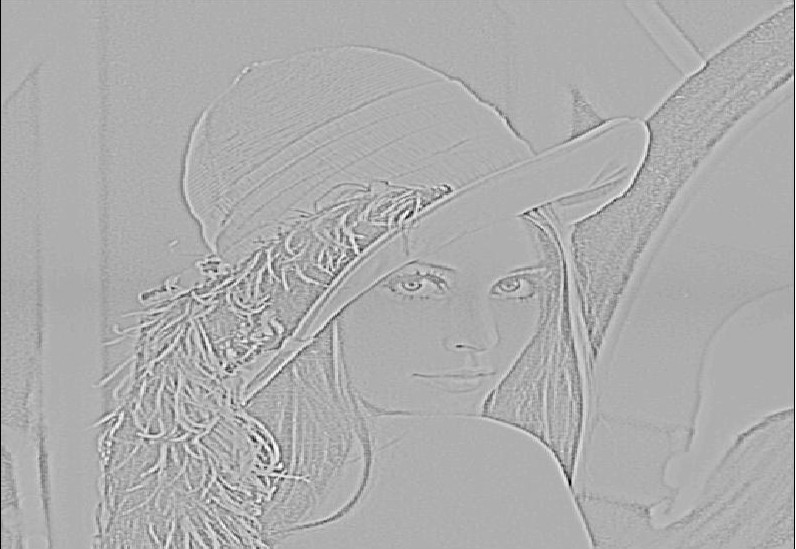
\includegraphics[width=21pc]{gfx/darkenedLennaLoG_LIP}\caption[LOG--LIP \texttt{Lenna} Oscurecida]{LoG--LIP sobre la imagen \texttt{Lenna} oscurecida.\label{fig:LogLIPlennaOscurecida}}
\end{SCfigure}
\begin{SCfigure}[][!t]
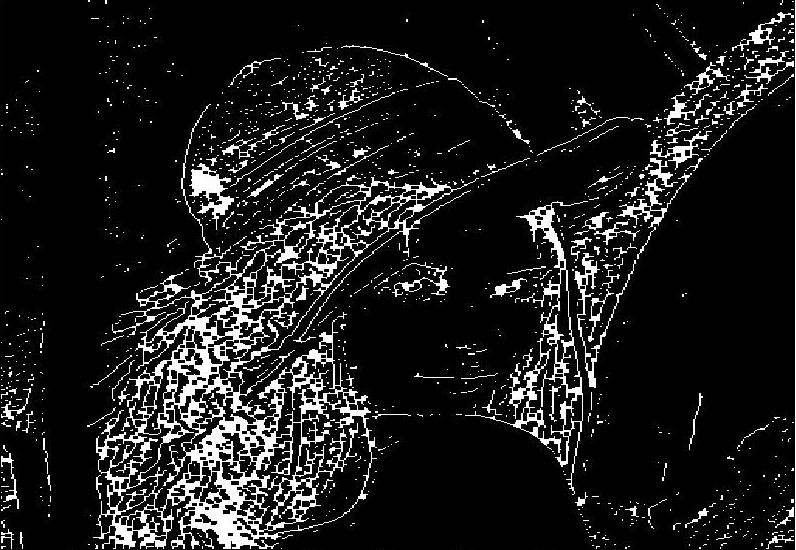
\includegraphics[width=21pc]{gfx/thresh10b_darkenedLennaLoG_LIP}\caption[LOG--LIP umbralizado Lenna Oscurecida]{LoG--LIP umbralizado (con $umbral = 10$) sobre la imagen \texttt{Lenna} oscurecida.\label{fig:threshLogLIPlennaOscurecida}}
\end{SCfigure}

\noindent Por el mismo motivo que en el caso del m�todo \emph{LIP--Sobel}, se ha comprobado el funcionamiento de estos operadores que se han descrito, utilizando una imagen conocida y de uso com�n, \texttt{Lenna} (Fig. \ref{fig:lennaOriginal}). Esta imagen ha sido modificada mediante la aplicaci�n una banda de oscurecimiento sobre los ojos (Fig. \ref{fig:lennaOscurecida}). Se ha calculado el filtro \emph{LoG} (con $\sigma = 1.0$) aplicando \eqref{eq:LoG_2D} sobre la imagen oscurecida, obteni�ndose la Fig. \ref{fig:LoGlennaOscurecida}, que ha sido umbralizada con un $umbral = 10$ y se ha generado la Fig. \ref{fig:threshLoGlennaOscurecida}. Por otra parte, se ha aplicado el operador \emph{LIP--LoG} (con $\sigma=1.0$), obteni�ndose Fig. \ref{fig:LogLIPlennaOscurecida}, que ha sido umbralizada tambi�n con un valor de $umbral = 10$ generando la Fig. \ref{fig:threshLogLIPlennaOscurecida}. Como se puede observar por simple inspecci�n, la imagen umbralizada tras el operador \emph{LIP--LoG} proporciona bordes en la zona oscurecida, frente a la imagen umbralizada tras aplicar el operador \emph{LoG}, el cual no obtiene bordes en dicha zona.
%\clearpage
\subsection{LIP--Canny}\label{sec:lipCanny}
El m�todo de \emph{Canny} \citep{canny86} es un m�todo muy robusto para la extracci�n de bordes en im�genes naturales que pueden tener presencia de ruido blanco gaussiano. En este apartado se propone un experimento que consiste en la aplicaci�n del paradigma \textsc{LIP} al extractor de bordes de \emph{Canny}. La adaptaci�n a \textsc{LIP} se realiza en los primeros pasos, la obtenci�n de los mapas de gradiente, en lugar de utilizar el operador \emph{convoluci�n} est�ndar se utiliza el operador \emph{Convoluci�n--\textsc{LIP}} expuesto en \eqref{eq:convLIPgt}. En el experimento realizado, se ha obtenido el mapa de bordes mediante tres mecanismos:
\begin{itemize}
\item Utilizando �nicamente el m�todo de \emph{Canny} tradicional.
\item Mediante una t�cnica h�brida en la que primero se aplica \emph{Filtrado Homom�rfico} y posteriormente el m�todo de \emph{Canny} tradicional.
\item A trav�s de un nuevo m�todo propuesto, \emph{LIP--Canny}.
\end{itemize}
\begin{SCfigure}[][!t]
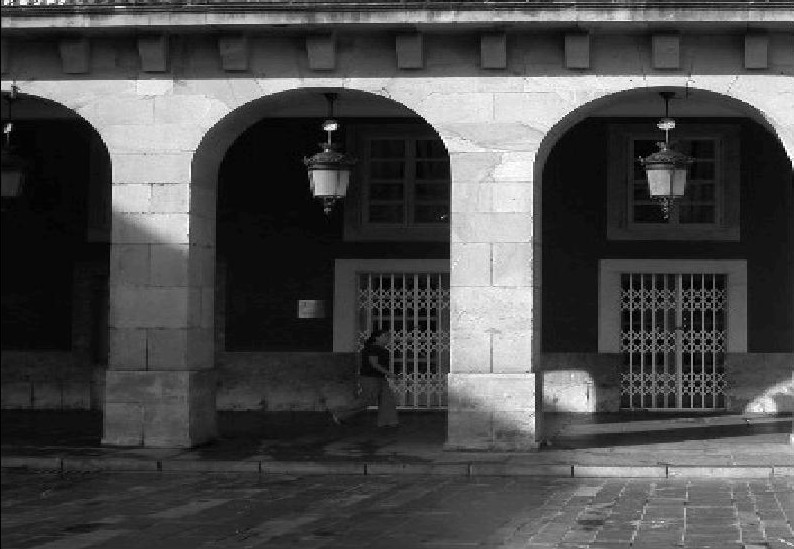
\includegraphics[width=21pc]{gfx/soportales.jpg}\caption[Sombras Original]{Imagen de un soportal con sombras naturales.\label{fig:soportales}}
\end{SCfigure}

\noindent Debido a la necesidad de comprobar el correcto funcionamiento en im�genes con sombras proyectadas reales, para este experimento se va a utilizar una de las im�genes seleccionadas en el Cap. \ref{chap:criterios}. Se ha escogido la \texttt{Imagen 4} del \textsc{dominio} \texttt{exteriores}, que se muestra en la Fig. \ref{fig:soportales}. Como puede observarse, esta imagen representa una fotograf�a de un soportal, parte del cual est� en sombras. Utilizando esta imagen, se ha obtenido la Fig. \ref{fig:soportalesCanny} que muestra los bordes mediante el m�todo tradicional de \emph{Canny}. La Fig. \ref{fig:soportalesFHCanny} contiene los contornos obtenidos mediante la aplicaci�n del \emph{Filtrado Homom�rfico} seguido del m�todo de \emph{Canny} habitual y por �ltimo, los bordes utilizando el nuevo m�todo propuesto \emph{LIP--Canny} se muestran en la Fig. \ref{fig:soportalesLIPCanny}. Para todos los m�todos se han utilizado los valores de los par�metros que han proporcionado en cada caso los mejores resultados, calculados estos mediante m�todos subjetivos. De manera com�n a todos los m�todos, se ha tomado \mbox{$\sigma$ = 1.0}, donde $\sigma$ es el valor de la amplitud de la campana de la gaussiana utilizada en las primeras fases de \emph{convoluci�n}.

\begin{SCfigure}[][!t]
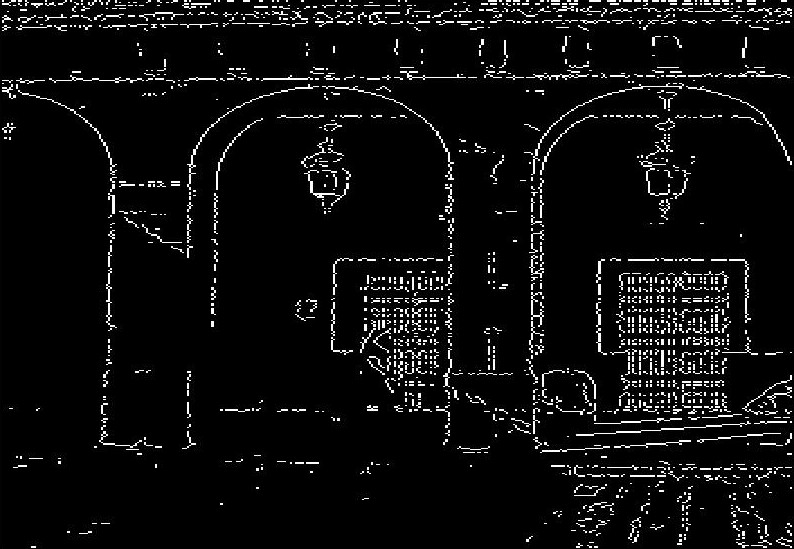
\includegraphics[width=21pc]{gfx/soportales_canny.jpg}\caption[Canny]{Mapa de bordes obtenidos utilizando \emph{Canny}. Par�metros: $\mathrm{th}_\mathrm{low} =$ 0.05, $\mathrm{th}_\mathrm{high} =$ 0.125.\label{fig:soportalesCanny}}
\end{SCfigure}
\begin{SCfigure}[][!t]
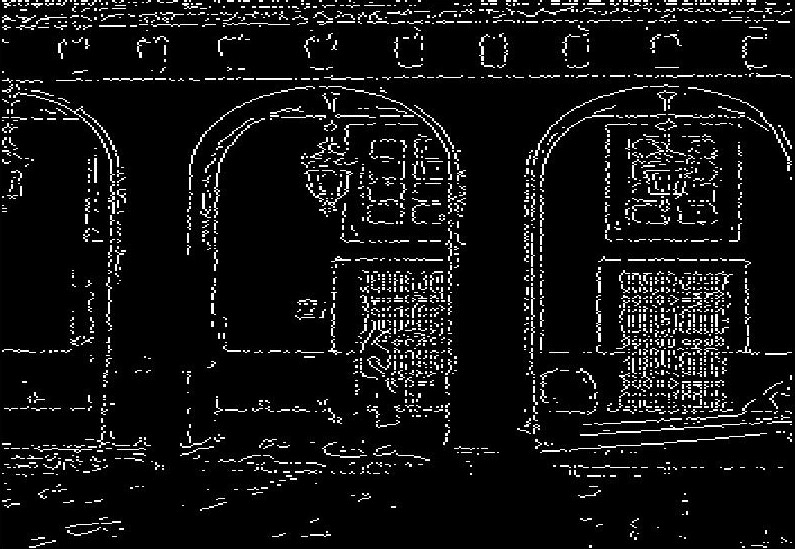
\includegraphics[width=21pc]{gfx/soportales_FH+Canny.jpg}\caption[\emph{Filtrado Homom�rfico}+Canny]{Mapa de bordes obtenidos utilizando \emph{Filtrado Homom�rfico} seguido de \emph{Canny}. Par�metros: $\mathrm{th}_\mathrm{low}=$ 0.01, \mbox{$\mathrm{th}_\mathrm{high} =$ 0.05.}\label{fig:soportalesFHCanny}}
\end{SCfigure}
\begin{SCfigure}[][!t]
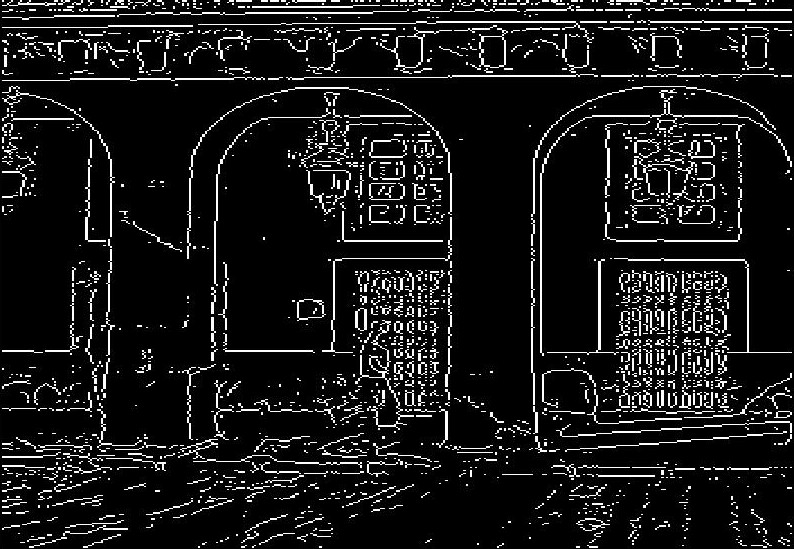
\includegraphics[width=21pc]{gfx/soportales_LIP-Canny.jpg}\caption[LIP--Canny]{Mapa de bordes obtenidos utilizando \emph{LIP--Canny}. Par�metros: $\mathrm{th}_\mathrm{low}=$ 0.05, \mbox{$\mathrm{th}_\mathrm{high} =$ 0.4.}\label{fig:soportalesLIPCanny}}
\end{SCfigure}
\FloatBarrier
\noindent Como se puede observar, el m�todo \emph{LIP--Canny} obtiene una mayor cantidad de bordes que el m�todo de \emph{Canny} para el mismo valor de umbral. Es m�s, el m�todo \emph{LIP--Canny} obtiene bordes precisos en la zona donde se proyecta la sombra, en la cual, el m�todo tradicional de \emph{Canny} no detecta ning�n borde. Para que el algoritmo tradicional de \emph{Canny} sea capaz de detectar dichos bordes, es necesario aplicar un paso previo de \emph{Filtrado Homom�rfico}. En este caso, el ajuste del umbral tiene que ser mucho m�s preciso, puesto que los valores del gradiente con los que opera \emph{Canny} tras el \emph{Filtrado Homom�rfico} son mucho m�s peque�os.\\
\noindent En la imagen de contornos obtenidos mediante \emph{LIP--Canny}, Fig. \ref{fig:soportalesLIPCanny}, se muestran los bordes de las cristaleras de la pared trasera de los soportales, que se encuentran en una zona de sombras en la imagen original, Fig. \ref{fig:soportales}. Por el contrario, en la Fig. \ref{fig:soportalesCanny}, que contiene el mapa de bordes obtenidos por \emph{Canny}, no aparecen esos mismos elementos.\\
\noindent Hay que indicar que los par�metros de los umbrales en el m�todo de \emph{LIP--Canny} son m�s altos que los mismos para el m�todo de \emph{Canny}, ya que para el mismo nivel de los umbrales, \emph{LIP--Canny} es capaz de detectar muchos m�s contornos que \emph{Canny}. Por otro lado, al aplicar el algoritmo compuesto por el \emph{Filtrado Homom�rfico} seguido del m�todo de \emph{Canny} aparece un gran problema de sensibilidad del umbral superior. Es decir, se dejan de detectar la gran mayor�a de bordes si se selecciona un umbral algo mayor que el �ptimo, y al contrario, se comienzan a detectar una cantidad excesiva de contornos en cuanto se desciende por debajo de dicho umbral. Lo que, en definitiva, hace que \emph{LIP--Canny} se pueda considerar como el mecanismo m�s robusto y vers�til de los 3 comparados en este experimento.
\section{Tiempos de c�mputo}\label{sec:tiemposComputo}
\lettrine{E}{n} las secciones anteriores, se ha mostrado que los algoritmos implementados mediante el operador propuesto \emph{Convoluci�n--\textsc{LIP}} presentan una respuesta visual mejor en todos los casos que los algoritmos equivalentes \textsc{No LIP}. En esta secci�n, se muestran los tiempos de c�mputo obtenidos para los diversos experimentos descritos con anterioridad y la comparaci�n de los diferentes m�todos en consideraci�n. En general, los tiempos de c�lculo que se muestran en este trabajo se han obtenido implementando todos los algoritmos y m�todos utilizando MATLAB\copyright 7 (R14) utilizando la Image Processing Toolbox y ejecutando los mismos en igualdad de carga computacional sobre un sistema Pentium\copyright Centrino M725 a 1.60 GHz (2MB L2--Cache) con 512 MB RAM.\\
\noindent Esta secci�n describe los resultados obtenidos en cada uno de los experimentos sin entrar en valoraciones o an�lisis de mayor profundidad, que se realizan en la Sec. \ref{sec:resumenResultados}.
\subsection{Aumento del rendimiento (\emph{Speedup})}
\noindent Adem�s de mostrar el tiempo de c�lculo de cada experimento, tambi�n se va a incluir otra medida, la ganancia de velocidad o \emph{Speedup}, que se nota como $S$, y se calcula mediante la siguiente f�rmula matem�tica:
\begin{equation}
S = \frac{\mathrm{T_{referencia}}}{\mathrm{T_{nuevo}}}\label{eq:speedup}
\end{equation}
\noindent Este t�rmino describe la velocidad relativa de un sistema nuevo ($\mathrm{T_{nuevo}}$) en relaci�n a otro sistema, que es tomado como referencia ($\mathrm{T_{referencia}}$). Si el valor de ganancia de velocidad es superior a uno, significa que el nuevo sistema es m�s r�pido que el de referencia; y al contrario, si el \emph{Speedup} es inferior a uno, el nuevo sistema se comporta de una manera m�s lenta que el de referencia.
\subsection{LIP--Sobel}
Se han realizado una serie de experimentos con \emph{LIP--Sobel}, que se han descrito anteriormente. En la Tab. \ref{tbl:timeLIPSobel} se muestra el tiempo de c�lculo para el algoritmo \emph{LIP--Sobel}, implementado en las tres versiones en consideraci�n (\person{Deng y Pinoli}, \mbox{\textsc{DGLIP--Conv}} y \mbox{\textsc{FGLIP--Conv}}) y con im�genes de dos tama�os diferentes ($512 \times 512$ y $320 \times 240$).\\
\noindent Aunque en la Sec. \ref{sec:lipsobelResultados} se realiza un an�lisis m�s profundo de estos datos, es conveniente indicar que para este experimento en particular, la versi�n m�s r�pida es la implementada utilizando \mbox{\textsc{FGLIP--Conv}}. Por el contrario, la versi�n de \emph{LIP--Sobel} mediante \mbox{\textsc{DGLIP--Conv}} es m�s lenta que la implementaci�n propuesta por \person{Deng y Pinoli}. Esta situaci�n ocurre debido a que, como se ha indicado en la Sec. \ref{sec:lipSobel}, la formulaci�n obtenida por \person{Deng y Pinoli} es una instanciaci�n concreta, optimizada para que dicha formulaci�n sea compacta. A su vez, dicha formulaci�n es equivalente a la obtenida por el m�canismo \mbox{\textsc{DGLIP--Conv}}, que sin embargo, es de car�cter general y no se encuentra optimizada para la minimizaci�n del n�mero de operaciones.
\begin{SCtable}[][!h]
\begin{tabular}{p{.3\textwidth}lll} \hline
\rowcolor{colorCorporativoSuave} \textsc{Algoritmo} & \textsc{Tama�o} & \textsc{M�todo} & \textsc{Tiempo} \\
\hline \hline
\cellcolor{colorCorporativoMedio} & \cellcolor{colorCorporativoMasSuave} & \cellcolor{colorCorporativoMasSuave} {Deng y Pinoli}      & \cellcolor{colorCorporativoMasSuave} 1.008 \\
\cline{3-4}
\cellcolor{colorCorporativoMedio} & \cellcolor{colorCorporativoMasSuave} & \cellcolor{colorCorporativoSuave} \mbox{\textsc{FGLIP--Conv}}  & \cellcolor{colorCorporativoSuave} 0.450 \\
\cline{3-4}
\cellcolor{colorCorporativoMedio} & \multirow{-3}{*}{\cellcolor{colorCorporativoMasSuave}$512 \times 512$} & \cellcolor{colorCorporativoMasSuave} \mbox{\textsc{DGLIP--Conv}}  & \cellcolor{colorCorporativoMasSuave} 5.847 \\
\cline{2-4}
\cellcolor{colorCorporativoMedio} & \cellcolor{colorCorporativoSuave} & \cellcolor{colorCorporativoSuave} {Deng y Pinoli}      & \cellcolor{colorCorporativoSuave} 0.386 \\
\cline{3-4}
\cellcolor{colorCorporativoMedio} & \cellcolor{colorCorporativoSuave} & \cellcolor{colorCorporativoMasSuave} \mbox{\textsc{FGLIP--Conv}}  & \cellcolor{colorCorporativoMasSuave} 0.155 \\
\cline{3-4}
\multirow{-6}{*}{\cellcolor{colorCorporativoMedio} LIP--Sobel}  & \multirow{-3}{*}{\cellcolor{colorCorporativoSuave}$320 \times 240$} & \cellcolor{colorCorporativoSuave} \mbox{\textsc{DGLIP--Conv}}  & \cellcolor{colorCorporativoSuave} 1.682 \\
\multicolumn{4}{p{0.95\textwidth}}{}\vspace{-1.5em}\\
\hline
\end{tabular}
\caption[Tiempos c�lculo]{Comparaci�n de tiempos de c�lculo (tiempo en segundos).\label{tbl:timeLIPSobel}}
\end{SCtable}

\subsubsection{Aumento del rendimiento (\emph{Speedup})}
\noindent En la Tab. \ref{tbl:speedupLIPSobel} se muestra el aumento del rendimiento de \emph{LIP--Sobel} implementado con \mbox{\textsc{FGLIP--Conv}} y \mbox{\textsc{DGLIP--Conv}}, en relaci�n con el m�todo original propuesto por \person{Deng y Pinoli}.
\begin{SCtable}[][!ht]
\begin{tabular}{p{0.2\textwidth}ccc} \hline
\rowcolor{colorCorporativoSuave} & & \multicolumn{2}{c}{\cellcolor{colorCorporativoSuave}\textsc{Speedup respecto Deng y Pinoli}}\\
\cline{3-4}
\rowcolor{colorCorporativoSuave} \textsc{Algoritmo}  & \textsc{Tama�o} & \mbox{\textsc{FGLIP--Conv}} & \mbox{\textsc{DGLIP--Conv}} \\
\hline \hline
\cellcolor{colorCorporativoMedio}            & \cellcolor{colorCorporativoMasSuave} $512\times 512$   & \cellcolor{colorCorporativoMasSuave} 2.24   & \cellcolor{colorCorporativoMasSuave} 0.17 \\
\cline{2-4}
\cellcolor{colorCorporativoMedio} \multirow{-2}{*}{LIP--Sobel} & \cellcolor{colorCorporativoSuave} $320\times 240$   & \cellcolor{colorCorporativoSuave} 2.49   & \cellcolor{colorCorporativoSuave} 0.23 \\
\multicolumn{4}{p{0.95\textwidth}}{}\vspace{-1.5em}\\
\hline
\end{tabular}
\caption[Speedup LIP--Sobel]{Speedup del \emph{LIP--Sobel} con respecto al mismo implementado mediante la t�cnica de \person{Deng y Pinoli}.\label{tbl:speedupLIPSobel}}
\end{SCtable}
\subsection{Algoritmos de emborronamiento: LIP--Avg, LIP--GBlur}
Los algoritmos de emborronamiento se han agrupado y se muestran tanto los tiempos de c�lculo como el \emph{Speedup} (este �ltimo siempre tomando como referencia el tiempo obtenido por el algoritmo implementado mediante la t�cnica de \person{Deng y Pinoli}). Se han realizado tres experimentos diferentes:
\begin{itemize}
\item Emborronamiento por filtro media de tama�o $3 \times 3$ p�xeles.
\item Emborronamiento por filtro media de tama�o $5 \times 5$ p�xeles.
\item Emborronamiento por filtro gaussiano de tama�o $7 \times 7$ p�xeles.
\end{itemize}
\noindent Estos experimentos se han realizado para dos tama�os de im�genes diferentes ($512 \times 512$ y $320 \times 240$ p�xeles). Y se han realizado mediante las tres t�cnicas \textsc{LIP} en consideraci�n:
\begin{itemize}
\item El m�todo propuesto por \person{Deng y Pinoli}.
\item Mediante \emph{Convoluci�n--LIP} implementado utilizando:
\begin{itemize}
\item \mbox{\textsc{DGLIP--Conv}}.
\item \mbox{\textsc{FGLIP--Conv}}.
\end{itemize}
\end{itemize}
\subsubsection{Tiempos de C�lculo}
En la Tab. \ref{tbl:timeBlur} se muestran los tiempos de los distintos experimentos sobre la misma arquitectura que la descrita para el experimento \emph{LIP--Sobel}. En esta tabla se vuelve a mostrar, que para todos los algoritmos de este experimento, las versiones m�s r�pidas son aquellas implementadas mediante \mbox{\textsc{FGLIP--Conv}}. Por el contrario, tanto para los algoritmos \emph{LIP--Avg (3$\times$ 3)} como para \emph{LIP--Avg (5$\times$ 5)}, al igual que ocurr�a en el experimento \emph{LIP--Sobel}, las implementaciones de los algoritmos que utilizan \mbox{\textsc{DGLIP--Conv}} son las m�s lentas. Sin embargo, para el algoritmo \emph{LIP--GBlur}, la implementaci�n mediante el mecanismo propuesto por \person{Deng y Pinoli} es claramente la m�s lenta, ya que no puede aprovecharse de la optimizaci�n y compactaci�n de la f�rmula matem�tica que trae dicha propuesta y, por el contrario, tanto \mbox{\textsc{FGLIP--Conv}} como \mbox{\textsc{DGLIP--Conv}} pueden hacer uso de la ventaja computacional que les ofrece la separabilidad de los filtros.
\begin{SCtable}[][!t]
\begin{tabular}{p{0.3\textwidth}lll} \hline
\rowcolor{colorCorporativoSuave}\textsc{Algoritmo} & \textsc{Tama�o} & \textsc{M�todo} & \textsc{Tiempo} \\
\hline \hline
\cellcolor{colorCorporativoMedio} & \cellcolor{colorCorporativoMasSuave} & \cellcolor{colorCorporativoMasSuave} {Deng y Pinoli} & \cellcolor{colorCorporativoMasSuave}0.456 \\
\cline{3-4}
\cellcolor{colorCorporativoMedio} & \cellcolor{colorCorporativoMasSuave} & \cellcolor{colorCorporativoSuave}\mbox{\textsc{FGLIP--Conv}}  & \cellcolor{colorCorporativoSuave}0.192 \\
\cline{3-4}
\cellcolor{colorCorporativoMedio} & \cellcolor{colorCorporativoMasSuave}\multirow{-3}{*}{$512 \times 512$} & \cellcolor{colorCorporativoMasSuave}\mbox{\textsc{DGLIP--Conv}}  & \cellcolor{colorCorporativoMasSuave}3.448 \\
\cline{2-4}
\cellcolor{colorCorporativoMedio} & \cellcolor{colorCorporativoSuave} & \cellcolor{colorCorporativoSuave} {Deng y Pinoli} & \cellcolor{colorCorporativoSuave}0.227 \\
\cline{3-4}
\cellcolor{colorCorporativoMedio} & \cellcolor{colorCorporativoSuave} & \cellcolor{colorCorporativoMasSuave}\mbox{\textsc{FGLIP--Conv}}  & \cellcolor{colorCorporativoMasSuave}0.076 \\
\cline{3-4}
\cellcolor{colorCorporativoMedio}\multirow{-6}{*}{LIP--Avg ($3 \times 3$)} &\cellcolor{colorCorporativoSuave}\multirow{-3}{*}{$320 \times 240$} & \cellcolor{colorCorporativoSuave}\mbox{\textsc{DGLIP--Conv}}  & \cellcolor{colorCorporativoSuave}1.017 \\
\hline
\cellcolor{colorCorporativoMedioSuave} & \cellcolor{colorCorporativoMasSuave} & \cellcolor{colorCorporativoMasSuave} {Deng y Pinoli} & \cellcolor{colorCorporativoMasSuave}0.482 \\
\cline{3-4}
\cellcolor{colorCorporativoMedioSuave} & \cellcolor{colorCorporativoMasSuave} & \cellcolor{colorCorporativoSuave}\mbox{\textsc{FGLIP--Conv}}  & \cellcolor{colorCorporativoSuave}0.198 \\
\cline{3-4}
\cellcolor{colorCorporativoMedioSuave} & \cellcolor{colorCorporativoMasSuave}\multirow{-3}{*}{$512 \times 512$} & \cellcolor{colorCorporativoMasSuave}\mbox{\textsc{DGLIP--Conv}}  & \cellcolor{colorCorporativoMasSuave}4.056 \\
\cline{2-4}
\cellcolor{colorCorporativoMedioSuave} & \cellcolor{colorCorporativoSuave} & \cellcolor{colorCorporativoSuave} {Deng y Pinoli} & \cellcolor{colorCorporativoSuave}0.246 \\
\cline{3-4}
\cellcolor{colorCorporativoMedioSuave} & \cellcolor{colorCorporativoSuave} & \cellcolor{colorCorporativoMasSuave}\mbox{\textsc{FGLIP--Conv}}  & \cellcolor{colorCorporativoMasSuave}0.077 \\
\cline{3-4}
\cellcolor{colorCorporativoMedioSuave}\multirow{-6}{*}{LIP--Avg ($5 \times 5$)} & \cellcolor{colorCorporativoSuave}\multirow{-3}{*}{$320 \times 240$}& \cellcolor{colorCorporativoSuave}\mbox{\textsc{DGLIP--Conv}} & \cellcolor{colorCorporativoSuave}1.189 \\
\hline
\cellcolor{colorCorporativoMedio} &\cellcolor{colorCorporativoMasSuave} & \cellcolor{colorCorporativoMasSuave} {Deng y Pinoli} & \cellcolor{colorCorporativoMasSuave}9.629 \\
\cline{3-4}
\cellcolor{colorCorporativoMedio} & \cellcolor{colorCorporativoMasSuave} & \cellcolor{colorCorporativoSuave}\mbox{\textsc{FGLIP--Conv}} & \cellcolor{colorCorporativoSuave}0.333 \\
\cline{3-4}
\cellcolor{colorCorporativoMedio} & \cellcolor{colorCorporativoMasSuave} \multirow{-3}{*}{$512 \times 512$} & \cellcolor{colorCorporativoMasSuave}\mbox{\textsc{DGLIP--Conv}}  & \cellcolor{colorCorporativoMasSuave}4.560 \\
\cline{2-4}
\cellcolor{colorCorporativoMedio} & \cellcolor{colorCorporativoSuave} & \cellcolor{colorCorporativoSuave} {Deng y Pinoli} & \cellcolor{colorCorporativoSuave}2.855 \\
\cline{3-4}
\cellcolor{colorCorporativoMedio} & \cellcolor{colorCorporativoSuave} & \cellcolor{colorCorporativoMasSuave}\mbox{\textsc{FGLIP--Conv}}  & \cellcolor{colorCorporativoMasSuave}0.175 \\
\cline{3-4}
\cellcolor{colorCorporativoMedio}\multirow{-6}{*}{LIP--GBlur} & \cellcolor{colorCorporativoSuave} \multirow{-3}{*}{$320 \times 240$}& \cellcolor{colorCorporativoSuave}\mbox{\textsc{DGLIP--Conv}} & \cellcolor{colorCorporativoSuave}1.421 \\
\multicolumn{4}{p{0.95\textwidth}}{}\vspace{-1.5em}\\
\hline
\end{tabular}
\caption[Tiempos c�lculo]{Comparaci�n de tiempos de c�lculo (tiempo en segundos).\label{tbl:timeBlur}}
\end{SCtable}
\subsubsection{Aumento del rendimiento (\emph{Speedup})}
De manera similar a lo expuesto en el experimento anterior, en la Tab. \ref{tbl:speedupBlur} se indica el \emph{Speedup}, tomando como referencia el tiempo de cada experimento implementado utilizando el m�todo propuesto por \person{Deng y Pinoli}.
\begin{SCtable}[][!ht]
\begin{tabular}{p{0.3\textwidth}ccc} \hline
\rowcolor{colorCorporativoSuave} & & \multicolumn{2}{c}{\cellcolor{colorCorporativoSuave}\textsc{Speedup respecto Deng y Pinoli}}\\
\cline{3-4}
\rowcolor{colorCorporativoSuave}\textsc{Algoritmo}  & \textsc{Tama�o} & \mbox{\textsc{FGLIP--Conv}} & \mbox{\textsc{DGLIP--Conv}} \\
\hline\hline
\cellcolor{colorCorporativoMedio} & \cellcolor{colorCorporativoMasSuave}$512\times 512$   & \cellcolor{colorCorporativoMasSuave}2.38   & \cellcolor{colorCorporativoMasSuave}0.13 \\
\cline{2-4}
\cellcolor{colorCorporativoMedio}\multirow{-2}{*}{LIP--Avg ($3\times 3$)} & \cellcolor{colorCorporativoSuave} $320\times 240$   & \cellcolor{colorCorporativoSuave}2.99   & \cellcolor{colorCorporativoSuave}0.22 \\
\hline
\cellcolor{colorCorporativoMedioSuave} & \cellcolor{colorCorporativoMasSuave}$512\times 512$   & \cellcolor{colorCorporativoMasSuave}2.43   & \cellcolor{colorCorporativoMasSuave}0.12 \\
\cline{2-4}
\cellcolor{colorCorporativoMedioSuave}\multirow{-2}{*}{LIP--Avg ($5\times 5$)} & \cellcolor{colorCorporativoSuave}$320\times 240$   & \cellcolor{colorCorporativoSuave}3.20   & \cellcolor{colorCorporativoSuave}0.21 \\
\hline
\cellcolor{colorCorporativoMedio} & \cellcolor{colorCorporativoMasSuave}$512\times 512$   & \cellcolor{colorCorporativoMasSuave}28.92  & \cellcolor{colorCorporativoMasSuave}2.11 \\
\cline{2-4}
\cellcolor{colorCorporativoMedio}\multirow{-2}{*}{LIP--GBlur} & \cellcolor{colorCorporativoSuave}$320\times 240$   & \cellcolor{colorCorporativoSuave}16.31  & \cellcolor{colorCorporativoSuave}2.01 \\
\multicolumn{4}{p{0.95\textwidth}}{}\vspace{-1.5em}\\
\hline
\end{tabular}
\caption[Speedup LIP--Avg, LIP--GBlur]{Speedup para cada experimento y m�todo con respecto al mismo implementado mediante la t�cnica de \person{Deng y Pinoli}.\label{tbl:speedupBlur}}
\end{SCtable}
\subsection{Extracci�n de bordes: LIP--LoG}
En este apartado se muestran los resultados obtenidos al implementar el algoritmo \emph{LIP--LoG}. Para este algoritmo se han realizado otros experimentos diferentes a los casos anteriores; se compara el algoritmo original \textsc{No LIP}, es decir, el algoritmo original \emph{LoG}, con los algoritmos \textsc{LIP} tanto por el m�todo de \person{Deng y Pinoli}, como por \emph{Convoluci�n--LIP} utilizando la aproximaci�n \mbox{\textsc{FGLIP--Conv}}, que se ha demostrado ser la aproximaci�n m�s r�pida. Las im�genes utilizadas tienen tama�os de $512 \times 512$ y de $256 \times 256$ p�xeles.
\subsubsection{Tiempo de C�lculo}
En la Tab. \ref{tbl:timeLoG} se muestran los tiempos de c�lculo para los diferentes experimentos. Se observa que \mbox{\textsc{FGLIP--Conv}} es la implementaci�n m�s r�pida, mientras que la implementaci�n mediante el mecanismo propuesto por \person{Deng y Pinoli} es la m�s lenta.
\begin{SCtable}[!ht]
\begin{tabular}{p{0.4\textwidth}lc} \hline
\rowcolor{colorCorporativoSuave}\textsc{Tama�o}    & \textsc{M�todo} & \textsc{Tiempo}\\
\hline\hline
\cellcolor{colorCorporativoMedio} & \cellcolor{colorCorporativoMasSuave}Standard LoG & \cellcolor{colorCorporativoMasSuave}0.1357\\
\cline{2-3}
\cellcolor{colorCorporativoMedio}$512 \times 512$ & \cellcolor{colorCorporativoSuave} {Deng y Pinoli} & \cellcolor{colorCorporativoSuave}7.8312\\
\cline{2-3}
\cellcolor{colorCorporativoMedio} & \cellcolor{colorCorporativoMasSuave}\mbox{\textsc{FGLIP--Conv}} & \cellcolor{colorCorporativoMasSuave}0.2163\\
\hline
\cellcolor{colorCorporativoMedioSuave} & \cellcolor{colorCorporativoSuave}Standard LoG & \cellcolor{colorCorporativoSuave}0.0390\\
\cline{2-3}
\cellcolor{colorCorporativoMedioSuave}$256 \times 256$ & \cellcolor{colorCorporativoMasSuave} {Deng y Pinoli} & \cellcolor{colorCorporativoMasSuave}1.2042\\
\cline{2-3}
\cellcolor{colorCorporativoMedioSuave} & \cellcolor{colorCorporativoSuave}\mbox{\textsc{FGLIP--Conv}} & \cellcolor{colorCorporativoSuave}0.0636\\
\multicolumn{3}{p{0.95\textwidth}}{}\vspace{-1.5em}\\
\hline
\end{tabular}
\caption[Tiempos LoG y LIP--LoG]{Comparaci�n de tiempos de c�lculo (tiempo en segundos) del experimento \emph{LoG} y \emph{LIP--LoG}.\label{tbl:timeLoG}}
\end{SCtable}
\subsubsection{Aumento del rendimiento (\emph{Speedup})}
Para este experimento se indican dos medidas de \emph{Speedup}. El primero, \textsc{Speedup d\&p.}, tomando como referencia el m�todo de \person{Deng y Pinoli}; mientras que el segundo (denominado \textsc{Speedup fg.}), toma como referencia el m�todo \mbox{\textsc{FGLIP--Conv}}. Los valores se muestran en la Tab. \ref{tbl:speedupLoG}.
\begin{SCtable}[][!ht]
\begin{tabular}{p{0.15\textwidth}lcc} \hline
\rowcolor{colorCorporativoSuave}\textsc{Tama�o}    & \textsc{M�todo} & \textsc{Speedup d\&p.} & \textsc{Speedup fg.}\\
\hline\hline
\cellcolor{colorCorporativoMedio} & \cellcolor{colorCorporativoMasSuave}Standard LoG               & \cellcolor{colorCorporativoMasSuave}57.71 & \cellcolor{colorCorporativoMasSuave}1.59\\
\cline{2-4}
\cellcolor{colorCorporativoMedio}$512 \times 512$ & \cellcolor{colorCorporativoSuave} {Deng y Pinoli}     & \cellcolor{colorCorporativoSuave}1.00  & \cellcolor{colorCorporativoSuave}0.03\\
\cline{2-4}
\cellcolor{colorCorporativoMedio} & \cellcolor{colorCorporativoMasSuave}\mbox{\textsc{FGLIP--Conv}}       & \cellcolor{colorCorporativoMasSuave}36.20 & \cellcolor{colorCorporativoMasSuave}1.00\\
\hline
\cellcolor{colorCorporativoMedioSuave} & \cellcolor{colorCorporativoSuave}Standard LoG               & \cellcolor{colorCorporativoSuave}30.88 & \cellcolor{colorCorporativoSuave}1.63\\
\cline{2-4}
\cellcolor{colorCorporativoMedioSuave}$256 \times 256$ & \cellcolor{colorCorporativoMasSuave} {Deng y Pinoli}     & \cellcolor{colorCorporativoMasSuave}1.00  & \cellcolor{colorCorporativoMasSuave}0.05\\
\cline{2-4}
\cellcolor{colorCorporativoMedioSuave} & \cellcolor{colorCorporativoSuave}\mbox{\textsc{FGLIP--Conv}}       & \cellcolor{colorCorporativoSuave}18.93 & \cellcolor{colorCorporativoSuave}1.00\\
\multicolumn{4}{p{0.95\textwidth}}{}\vspace{-1.5em}\\
\hline
\end{tabular}
\caption[Speedup LoG y LIP--LoG]{Comparaci�n de \emph{Speedup} del experimento \emph{LoG} y  \emph{LIP--LoG}.\label{tbl:speedupLoG}}
\end{SCtable}
\subsection{Extracci�n de bordes: LIP--Canny}
Este experimento, en el que se utiliza el algoritmo de extracci�n de bordes de \emph{Canny}, compara dos aproximaciones invariantes ante cambios de iluminaci�n y la versi�n original del algoritmo. Las dos aproximaciones invariantes ante cambios de iluminaci�n son:
\begin{itemize}
\item El algoritmo \emph{LIP--Canny} utilizando \mbox{\textsc{FGLIP--Conv}}, tal y como se ha indicado en Sec. \ref{sec:lipCanny}.
\item Un preprocesamiento previo de la imagen mediante \emph{Filtrado Homom�rfico} y posterior aplicaci�n del algoritmo est�ndar de \emph{Canny} sobre la imagen reflectancia obtenida del paso de preprocesamiento anterior.
\end{itemize}
\noindent Las im�genes son diferentes de las utilizadas con anterioridad, ya que deb�an incluir sombras proyectadas naturales. Estas nuevas im�genes tienen tama�os de $425\times 640$ y $374\times 353$ p�xeles, respectivamente.
\subsubsection{Tiempo de C�lculo}
En la Tab. \ref{tab:timeLIPCanny} se muestran los tiempos de c�lculo para cada uno de los experimentos e im�genes. En este experimento, la versi�n m�s r�pida es la que aplica \emph{Canny} directamente, aunque como se ha indicado en la Sec. \ref{sec:lipCanny}, �sta no es capaz de proporcionar los contornos de las zonas en sombras. Entre las dos implementaciones que permiten la obtenci�n de los bordes de las zonas oscuras, el m�todo \emph{LIP--Canny} es m�s r�pido que el mecanismo h�brido constituido por la aplicaci�n de un \emph{Filtrado Homom�rfico} seguido del algoritmo de \emph{Canny}, notado como \emph{F.H. + Canny}.
\begin{SCtable}[][!ht]
\begin{tabular}{p{0.4\textwidth}cc} \hline
\rowcolor{colorCorporativoSuave}\textsc{Tama�o} & \textsc{M�todo} & \textsc{Tiempo}\\
\hline\hline
\cellcolor{colorCorporativoMedio} & \cellcolor{colorCorporativoMasSuave}Canny & \cellcolor{colorCorporativoMasSuave}1.190\\
\cline{2-3}
\cellcolor{colorCorporativoMedio}$425\times 640$ & \cellcolor{colorCorporativoSuave}F.H. + Canny & \cellcolor{colorCorporativoSuave}1.341\\
\cline{2-3}
\cellcolor{colorCorporativoMedio} & \cellcolor{colorCorporativoMasSuave}\emph{LIP--Canny} & \cellcolor{colorCorporativoMasSuave}\textsc{1.250}\\
\hline
\cellcolor{colorCorporativoMedioSuave}  & \cellcolor{colorCorporativoSuave}Canny & \cellcolor{colorCorporativoSuave}0.519\\
\cline{2-3}
\cellcolor{colorCorporativoMedioSuave}$374\times 353$ & \cellcolor{colorCorporativoMasSuave}F.H. + Canny & \cellcolor{colorCorporativoMasSuave}0.623\\
\cline{2-3}
\cellcolor{colorCorporativoMedioSuave} & \cellcolor{colorCorporativoSuave}\emph{LIP--Canny} & \cellcolor{colorCorporativoSuave}\textsc{0.585}\\
\multicolumn{3}{p{0.95\textwidth}}{}\vspace{-1.5em}\\
\hline
\end{tabular}
\caption[Tiempos Canny, LIP--Canny y FH+Canny]{Tiempos de procesamiento para \emph{Canny}, \emph{LIP--Canny} y Filtrado Homom�rfico (F.H.) seguido de \emph{Canny}.\label{tab:timeLIPCanny}}
\end{SCtable}
\subsubsection{Aumento del rendimiento (\emph{Speedup})}
En la Tab. \ref{tab:speedupLIPCanny} se muestra el \emph{Speedup} de cada uno de los algoritmos, tomando el \emph{LIP--Canny} como sistema de referencia para cada tama�o de imagen.
\begin{SCtable}[][!ht]
\begin{tabular}{p{0.4\textwidth}cc} \hline
\rowcolor{colorCorporativoSuave}\textsc{Tama�o} & \textsc{M�todo} & \textsc{Speedup}\\
\hline\hline
\cellcolor{colorCorporativoMedio} & \cellcolor{colorCorporativoMasSuave}Canny & \cellcolor{colorCorporativoMasSuave}0.952\\
\cline{2-3}
\cellcolor{colorCorporativoMedio}$425\times 640$ & \cellcolor{colorCorporativoSuave}F.H. + Canny & \cellcolor{colorCorporativoSuave}1.073 \\
\cline{2-3}
\cellcolor{colorCorporativoMedio} & \cellcolor{colorCorporativoMasSuave}\emph{LIP--Canny} & \cellcolor{colorCorporativoMasSuave}\textsc{1.0} \\
\hline
\cellcolor{colorCorporativoMedioSuave} & \cellcolor{colorCorporativoSuave}Canny & \cellcolor{colorCorporativoSuave}0.887\\
\cline{2-3}
\cellcolor{colorCorporativoMedioSuave}$374\times 353$ & \cellcolor{colorCorporativoMasSuave}F.H. + Canny & \cellcolor{colorCorporativoMasSuave}1.065\\
\cline{2-3}
\cellcolor{colorCorporativoMedioSuave} & \cellcolor{colorCorporativoSuave}\emph{LIP--Canny} & \cellcolor{colorCorporativoSuave}\textsc{1.0}\\
\multicolumn{3}{p{0.95\textwidth}}{}\vspace{-1.5em}\\
\hline
\end{tabular}
\caption[Speedup Canny, LIP--Canny y FH+Canny]{\emph{Speedup} para \emph{Canny}, \emph{LIP--Canny} y Filtrado Homom�rfico (F.H.) seguido de \emph{Canny}.\label{tab:speedupLIPCanny}}
\end{SCtable}

\section{Resumen de resultados}\label{sec:resumenResultados}
\lettrine{A}{nalizando} los resultados obtenidos se puede estimar la calidad de los m�todos propuestos, al menos, desde un punto de vista de eficiencia computacional y de tiempo de procesamiento. En los siguientes apartados, se van a tratar cada uno de los experimentos, calculando en cada caso el aumento de rendimiento general de cada implementaci�n.
\subsection{LIP--Sobel}\label{sec:lipsobelResultados}
\noindent Si se toma �nicamente el aspecto visual, se puede observar que el algoritmo est�ndar de \emph{Sobel} no es capaz de mostrar claramente los contornos de las zonas m�s oscuras, mientras que la implementaci�n \emph{LIP--Sobel} s� que muestra los bordes de toda la imagen, de manera independiente al grado de iluminaci�n local.\\
\noindent Con respecto al tiempo de procesamiento y al aumento de rendimiento, la ganancia media del experimento implementado mediante \textsc{FGLIP--Conv} es aproximadamente de $2.5$ veces m�s que el mismo implementado por el m�todo de \person{Deng y Pinoli}. Mientras que, en cambio, el \emph{LIP--Sobel} utilizando el m�todo \textsc{DGLIP--Conv} es m�s lento que el mismo siguiendo la propuesta de \person{Deng y Pinoli}, ya que se obtiene un \emph{Speedup} de $0.21$, es decir, es aproximadamente un $80\%$ m�s lento.\\
\noindent Este experimento requiere un an�lisis m�s profundo de los resultados temporales, ya que a pesar de que la versi�n \textsc{DGLIP--Conv} del algoritmo \emph{LIP--Sobel} utiliza un mecanismo de \emph{convoluci�n} por filtros separables, es m�s lenta que la implementada mediante el mecanismo propuesto por \person{Deng y Pinoli}, que utiliza filtros bidimensionales, que har�a que su aplicaci�n fuese te�ricamente m�s lenta. La lentitud de la propuesta \textsc{DGLIP--Conv} viene dada por dos factores: la elevada carga computacional de los operadores multiplicaci�n y potenciaci�n, y el hecho de que el filtro bidimensional de Sobel contiene muchos valores a $0$. Esta segunda caracter�stica hace que, para cada p�xel, la aplicaci�n del filtro bidimensional de \emph{LIP--Sobel} mediante el mecanismo propuesto por \person{Deng y Pinoli} se realice con seis multiplicaciones, una divisi�n y dos potenciaciones al cuadrado (que podr�an implementarse mediante dos multiplicaciones o de manera a�n m�s efectiva mediante un desplazamiento binario de un bit hacia la izquierda). Por tanto, tomando de manera simplificada que el tama�o de la imagen es de $n \times n$ p�xeles, la aplicaci�n de \emph{LIP--Sobel} seg�n el m�todo propuesto por \person{Deng y Pinoli} proporciona 18 operaciones por p�xel, como muestra \eqref{eq:compLIPSobelDP}. En cualquier caso, se necesita el doble de las operaciones descritas ya que para obtener \emph{LIP--Sobel} hay que aplicar dos filtros bidimensionales para el c�lculo de la imagen gradiente. Para poder proporcionar datos a�n m�s precisos, se ha podido estimar que el operador potenciaci�n es cinco veces m�s lento que el operador multiplicaci�n, por tanto, para poder realizar comparaciones, se va a calcular el n�mero de \emph{operaciones equivalentes} (oper. eq.) de cada implementaci�n. La normalizaci�n en \emph{operaciones equivalentes} hace que una potenciaci�n sea igual a 5 oper. eq. y que 1 multiplicaci�n o divisi�n coincida con 1 oper. eq.
\begin{eqnarray}
&\mathrm{N�mero\ de\ operaciones\ de\ LIP-Sobel}_\mathrm{Deng\& Pinoli}: \nonumber\\
&2 \times \left( n^2\times\left(6\ \mathrm{multip.} + 1\ \mathrm{divis.} + 2\ \mathrm{potenc.}\right)\right) \Rightarrow \nonumber\\
& 2\times n^2\times 9\ \mathrm{oper.} \Rightarrow 18n^2\ \mathrm{oper.} \Rightarrow 34n^2\ \mathrm{oper.\ eq.}&\label{eq:compLIPSobelDP}
\end{eqnarray}

\noindent Sin embargo, la implementaci�n de \emph{LIP--Sobel} utilizando \textsc{DGLIP--Conv} requiere, para una imagen de igual tama�o, una doble aplicaci�n de 3 multiplicaciones y 3 potenciaciones por filtro. En \eqref{eq:compLIPSobelDGLIPConv} se muestra la estimaci�n del n�mero de operaciones requeridas para dicha implementaci�n, en la que el n�mero de operaciones por p�xel es menor que en el caso anterior, pero el n�mero total para la imagen completa es mayor. Tambi�n se indica el n�mero de \emph{operaciones equivalentes}.
\begin{eqnarray}
&\mathrm{N�mero\ de\ operaciones\ de\ LIP-Sobel}_\mathrm{DGLIP-Conv}: \nonumber\\
&2 \times \left( 2 \times \left(n^2\times\left(3\ \mathrm{multip.} + 3\ \mathrm{potenc.}\right)\right)\right) \Rightarrow & \nonumber\\
& 4\times n^2\times 6\ \mathrm{oper.} \Rightarrow 24n^2\ \mathrm{oper.} \Rightarrow 72n^2\ \mathrm{oper.\ eq.}&\label{eq:compLIPSobelDGLIPConv}
\end{eqnarray}

\noindent Para \textsc{DGLIP--Conv}, el c�lculo utiliza un filtro en el que cada elemento del mismo tiene un valor diferente no nulo, por lo cual, no es posible realizar ninguna optimizaci�n para obtener una reducci�n en el n�mero de potenciaciones (que es la operaci�n computacionalmente m�s costosa). Como se podr� comprobar en otros experimentos, en cuanto los filtros que se aplican tienen un mayor tama�o y est�n compuestos por valores no uniformes y no nulos, la ventaja de la propuesta de \person{Deng y Pinoli} se esfuma y la implementaci�n \textsc{DGLIP--Conv} tambi�n muestra una mejora en los tiempos de ejecuci�n frente a dicha propuesta.
\subsection{LIP--Avg, LIP--GBlur}\label{lipavglipgblurResultados}
\noindent Como se ha comentado a lo largo del cap�tulo, estos dos experimentos muestran los dos extremos de \emph{caso m�s favorable} y \emph{m�s desfavorable} para el m�todo propuesto por \person{Deng y Pinoli}. El algoritmo \emph{LIP--Avg} realiza el filtro \emph{media} y se corresponde con el ``mejor caso'', ya que se puede obtener un exponente com�n para todos los p�xeles. Frente a este caso se encuentra el del algoritmo \emph{LIP--GBLur}, que aplica un filtrado gaussiano y es el ``peor caso'', ya que no es posible sacar un exponente com�n y hay que elevar cada p�xel a un exponente diferente. Si se calcula el \emph{Speedup} de cada experimento, seg�n tama�o de imagen y de filtro, de la implementaci�n utilizando el m�todo propuesto por \person{Deng y Pinoli} frente a las implementaciones de los mismos utilizando \textsc{DGLIP--Conv} y \textsc{FGLIP--Conv}, se puede observar que para el experimento \emph{LIP--Avg} es de $2.75$ y de $0.17$, respectivamente. Por otra parte, para el experimento \emph{LIP--GBLur} se obtiene un aumento del rendimiento de $22.62$ para \textsc{FGLIP--Conv} y de $2.06$ para \textsc{DGLIP--Conv}. As�, en general, el \emph{Speedup} medio para los dos experimentos (para todos los tama�os de imagen y de filtros) del m�todo \textsc{FGLIP--Conv} es de $9.38$; mientras que el \emph{Speedup} medio de los experimentos implementados utilizando \textsc{DGLIP--Conv} alcanza un modesto $0.80$. Esto demuestra que la implementaci�n mediante \textsc{FGLIP--Conv} es m�s r�pida que el mecanismo propuesto por \person{Deng y Pinoli}, mientras que la implementaci�n mediante \textsc{DGLIP--Conv} se comporta de forma m�s lenta.\\
\noindent En el experimento \emph{LIP--Avg ($3\times 3$)}, el denominado ``mejor caso'' para el mecanismo propuesto por \person{Deng y Pinoli}, se aplican 9 multiplicaciones y una potenciaci�n (10 operaciones) por cada p�xel, por lo tanto, esta implementaci�n requiere 14 \emph{operaciones equivalentes}.
\begin{eqnarray}
&\mathrm{N�mero\ de\ operaciones\ de\ LIP-Avg}(3\times 3)_\mathrm{Deng\& Pinoli}: \nonumber\\
&n^2\times\left(9\ \mathrm{multip.} + 1\ \mathrm{potenc.}\right) \Rightarrow 10n^2\ \mathrm{oper.} \Rightarrow 14n^2\ \mathrm{oper.\ eq.}&\nonumber \\ \label{eq:compLIPavgTresDP}
\end{eqnarray}

\noindent Por otra parte, en el m�todo \textsc{DGLIP--Conv} se necesitan 3 multiplicaciones y 3 potenciaciones, pero hay que aplicar dos veces dicho filtrado (12 operaciones) en cada p�xel, que implican 36  \emph{operaciones equivalentes}. En \eqref{eq:compLIPavgTresDP} y \eqref{eq:compLIPavgTresDGLIPConv}, se muestran respectivamente los c�lculos del n�mero de operaciones aplicadas en ambos m�todos.
\begin{eqnarray}
&\mathrm{N�mero\ de\ operaciones\ de\ LIP-Avg}(3\times 3)_\mathrm{DGLIP-Conv}: \nonumber\\
&2 \times \left( n^2\times\left(3\ \mathrm{multip.} + 3\ \mathrm{potenc.}\right)\right) \Rightarrow \nonumber\\
& 2\times n^2\times 6\ \mathrm{oper.} \Rightarrow 12n^2\ \mathrm{oper.} \Rightarrow 36n^2\ \mathrm{oper.\ eq.}&\label{eq:compLIPavgTresDGLIPConv}
\end{eqnarray}

%\noindent Para el experimento \emph{LIP--Avg ($5 \times 5$)}, la implementaci�n propuesta por \person{Deng y Pinoli} utiliza 25 multiplicaciones y una potenciaci�n (26 operaciones) frente a las 5 multiplicaciones y 5 potenciaciones (20 operaciones) que efect�a el m�todo \textsc{DGLIP--Conv}. En ambos algoritmos, el m�todo propuesto por \person{Deng y Pinoli} puede aprovechar la existencia de un factor com�n, que reduce el n�mero de potenciaciones necesarias a tan s�lo una. Por el contrario, \textsc{DGLIP--Conv} realiza tantas potenciaciones como elementos tienen los filtros aplicados y no puede reducir su n�mero de operaciones. El hecho de que aplique filtros separables no consigue reducir suficientemente el tiempo de c�mputo, ya que pesa mucho m�s el gasto computacional por el n�mero de operaciones que ha de aplicar.\\
\noindent Por el contrario, en el �ltimo experimento \emph{LIP--GBlur}, la implementaci�n mediante el mecanismo propuesto por \person{Deng y Pinoli} utiliza 49 multiplicaciones y 49 potenciaciones (98 operaciones) para calcular cada nuevo p�xel, tal y como se muestra en \eqref{eq:compLIPgblurDP}, la cantidad de operaciones totales es de $294n^2$ \emph{operaciones equivalentes}.
\begin{eqnarray}
&\mathrm{N�mero\ de\ operaciones\ de\ LIP-GBlur}_\mathrm{Deng\& Pinoli}: \nonumber\\
& n^2\times\left(49\ \mathrm{multip.} + 49\ \mathrm{potenc.}\right) \Rightarrow 98n^2\ \mathrm{oper.} \Rightarrow 294n^2\ \mathrm{oper.\ eq.}& \nonumber \\ \label{eq:compLIPgblurDP}
\end{eqnarray}

\noindent Mientras que para la versi�n que utiliza \textsc{DGLIP--Conv}, la cantidad de operaciones se reduce a 7 multiplicaciones y 7 potenciaciones por p�xel y filtro. En \eqref{eq:compLIPgblurDGLIPConv} se muestra que el n�mero de \emph{operaciones equivalentes} total es de $84n^2$.
\begin{eqnarray}
&\mathrm{N�mero\ de\ operaciones\ de\ LIP-GBlur}_\mathrm{DGLIP-Conv}: \nonumber\\
&2 \times \left( n^2\times\left(7\ \mathrm{multip.} + 7\ \mathrm{potenc.}\right)\right) \Rightarrow \nonumber\\
& 2\times n^2\times 14\ \mathrm{oper.} \Rightarrow 28n^2\ \mathrm{oper.} \Rightarrow 84n^2\ \mathrm{oper.\ eq.}&\label{eq:compLIPgblurDGLIPConv}
\end{eqnarray}

\noindent En este caso, el hecho de que \textsc{DGLIP--Conv} haga uso de un menor n�mero de operaciones unido al uso de los filtros separables, tiene mayor importancia. Gracias a una mejor pol�tica de acceso (debido a un menor n�mero de fallos de cach�), esta implementaci�n consigue batir holgadamente al m�todo propuesto por \person{Deng y Pinoli}.
\subsection{LIP--LoG}\label{sec:liplogResultados}
\noindent Tras observar en los experimentos anteriores que \textsc{FGLIP--Conv} es el m�todo m�s r�pido para la implementaci�n del operador \emph{Convoluci�n--LIP}, para este algoritmo (\emph{LIP--LoG}) s�lo se han realizado pruebas mediante el algoritmo \emph{LoG} est�ndar (no \textsc{LIP}), \emph{LIP--LoG} implementado mediante la t�cnica adaptada de la propuesta de \person{Deng y Pinoli} y \emph{LIP--LoG} implementado utilizando \textsc{FGLIP--Conv}. En general, se puede observar que \emph{LIP--LoG} es capaz de detectar bordes en zonas oscurecidas, mientras que el algoritmo \emph{LoG} est�ndar no es capaz de encontrar dichos contornos. Por lo que, en el aspecto temporal, aunque \emph{LoG} es el algoritmo que menos tarda, no proporciona una respuesta satisfactoria, al perderse contornos de zonas oscuras, que s� son detectados por \emph{LIP--LoG}. Particularizando en las dos implementaciones del \emph{LIP--LoG}, que son mediante el m�todo de \person{Deng y Pinoli} y mediante \textsc{FGLIP--Conv}, se obtienen las siguientes medidas de ganancia de velocidad: \textsc{FGLIP--Conv} es aproximadamente un $60\%$ m�s lento que el algoritmo b�sico de \emph{LoG}, mientras que es entre un $200\%$ y un $350\%$ m�s r�pido que el m�todo propuesto por \person{Deng y Pinoli}.
\subsection{LIP--Canny}\label{lipcannyResultados}
\noindent Como ya se ha comentado en la Sec. \ref{sec:lipCanny}, el algoritmo de \emph{Canny} no es capaz de detectar contornos en las zonas oscuras ni en las sombras proyectadas, sin embargo, la implementaci�n de \emph{LIP--Canny} realizada mediante \textsc{FGLIP--Conv} obtiene todos los contornos de los elementos de dichas zonas. Por tanto, se puede afirmar que \emph{LIP--Canny} mejora el funcionamiento general del m�todo de \emph{Canny}.\\% y es m�s robusto y f�cil de ajustar que si se realiza un \emph{Filtrado Homom�rfico} seguido de una extracci�n mediante el m�todo de \emph{Canny}.\\ % Para que el m�todo de \emph{Canny} sea capaz de obtener resultados similares, es necesaria aplicar una fase previa de \emph{Filtrado Homom�rfico}.  
\noindent Con respecto a los tiempos de c�mputo, se han realizado experimentos para dos tama�os distintos (la de tama�o menor, es una imagen recortada de la mayor). El tiempo de c�lculo de \emph{Canny} es aproximadamente entre un $14 \%$ y un $5 \%$ m�s r�pido que el de \emph{LIP--Canny} y esto es debido a que para calcular \emph{LIP--Canny} se realizan una serie de operaciones adicionales, frente a la \emph{convoluci�n} simple que se realiza en el m�todo de \emph{Canny}. Para obtener una soluci�n similar, a la cual no le afecten los cambios de iluminaci�n, como se ha visto anteriormente, habr��a que aplicar un \emph{Filtrado Homom�rfico}. Esto aumenta el tiempo de c�mputo con respecto a la aplicaci�n directa del m�todo de \emph{Canny}. Por los experimentos realizados, se ha obtenido que la aplicaci�n de un \emph{Filtrado Homom�rfico} seguido del m�todo de \emph{Canny} es entre un $13 \%$ y $20 \%$ m�s lento que aplicar �nicamente el m�todo de \emph{Canny}.\\
\noindent Para este experimento, se ha calculado el \emph{Speedup} tomando como tiempo de referencia, seg�n el tama�o de la imagen, el resultado de tiempos de la aplicaci�n del m�todo propuesto de \emph{LIP--Canny}. Se puede observar, que el m�todo h��brido (primero, \emph{Filtrado Homom�rfico} y posteriormente, el m�todo de \emph{Canny}) es entre un $6.5$ y un $7.3\%$ m�s lento que \emph{LIP--Canny}. Por lo tanto, tambi�n se puede afirmar que ambas implementaciones proporcionan resultados equiparables entre s�, aunque el mecanismo h�brido es m�s lento y el ajuste del umbral de los par�metros para dicho m�todo es mucho m�s sensible a peque�as modificaciones que en el caso de \emph{LIP--Canny}, que se comporta de forma m�s robusta.
\section{Conclusiones}
\lettrine{E}{n} los apartados anteriores se ha mostrado el nuevo operador propuesto (\mbox{\emph{Convoluci�n--LIP}}), que puede ser implementado mediante dos versiones diferentes (\mbox{\textsc{DGLIP--Conv}} y \mbox{\textsc{FGLIP--Conv}}). Con ellos se ha podido observar que se puede generalizar de manera simple y efectiva cualquier algoritmo de procesamiento de im�genes al paradigma \textsc{LIP} siempre que se utilicen filtros de \emph{convoluci�n} separables. Aunque en trabajos previos \citep{deng98}, otros autores hab�an dejado entrever un posible m�todo para este fin, el operador que se propone en esta Tesis Doctoral es m�s vers�til, puesto que permite adaptar cualquier filtro sin necesidad de recodificaci�n.\\
\noindent Adem�s, se han mostrado los tiempos de c�mputo de los distintos experimentos. En ellos, se ha demostrado que las implementaciones de los algoritmos realizadas mediante \mbox{\textsc{FGLIP--Conv}} son las m�s r�pidas, logr�ndose aumentos de velocidad (\emph{Speedup}) medias de $200\%$, es decir, el doble de r�pido que otras implementaciones. En algunos experimentos se han obtenido aumentos de velocidad de m�s de $3600\%$.
\myChapter{Resultados de los cuestionarios de calidad de bordes}\label{chap:resultadosCuestionarios}
\minitoc\mtcskip
\vfill
\lettrine{U}{na} de las facetas m�s singulares del ser humano, que ha marcado su evoluci�n, ha sido la b�squeda del �ptimo en todos los �mbitos de inter�s. Cuando no se puede obtener dicho �ptimo, se buscan los m�todos que proporcionen los mejores resultados relativos. Sin embargo, cuando la determinaci�n del mejor caso no es f�cil de obtener o cuando depende de factores subjetivos no mesurables, el mejor sistema para obtener la calificaci�n es mediante cuestionarios de evaluaci�n. Un claro ejemplo de la utilidad de este sistema se expone en este cap�tulo, en el que se utilizan dos encuestas para evaluar la calidad de 6 m�todos de extracci�n de bordes diferentes con 2 par�metros de funcionamiento diferentes.
\clearpage
\section{Cuestionarios para evaluaci�n de contornos}
\lettrine{C}{omo} se ha comentado a lo largo de esta Tesis, la calidad de los contornos es un concepto con un alto grado de subjetividad: algunos usuarios pueden preferir contornos suaves aunque menos precisos y otros pueden preferir contornos con muy alta precisi�n aunque sean m�s abruptos. Es m�s, la subjetividad no s�lo depende de la persona sino tambi�n de la utilidad o tarea visual que se desee obtener a partir de dichos contornos: una misma persona puede escoger un mapa de contornos para una determinada tarea y para otra tarea distinta escoger otro mapa de contornos diferente. Por todo esto, se ha determinado que la mejor opci�n para identificar el algoritmo de extracci�n de bordes que proporcione el conjunto de contornos globalmente m�s aceptado es mediante cuestionarios de opini�n.\\
\noindent La construcci�n de una herramienta �nica para la investigaci�n mediante encuestas de im�genes de contornos es un objetivo que excede el �mbito de esta Tesis. Adem�s, proporcionar una encuesta capaz de evaluar todo tipo de m�todos de contornos, de cualquier dominio de im�genes y para cualquier poblaci�n es poco realista. M�s a�n cuando ni existen metodolog�as de dise�o de encuestas en este sentido, ni se han desarrollado encuestas previas con las que comparar. Esta Tesis pretende abrir un camino robusto y con indicios de veracidad cient�fica en el dise�o y utilizaci�n de encuestas para el an�lisis de la calidad de los m�todos de extracci�n de contornos en im�genes.
\noindent En este cap�tulo se muestran los resultados obtenidos a partir de la evaluaci�n subjetiva de la calidad percibida de diferentes algoritmos de extracci�n de contornos. Sin embargo, en este cap�tulo, no s�lo se proporcionan resultados estr�ctamente num�ricos, sino que tambi�n se aportan como resultados de la investigaci�n, toda la informaci�n del proceso completo de dise�o de los cuestionarios, de la puesta en marcha y de la fase de recolecci�n de respuestas utilizando el sistema Web descrito en el Cap. \ref{chap:recCuestCalidadBordes}. Dentro del �mbito de la evaluaci�n subjetiva de im�genes y de v�deo, existen procedimientos regulados \cite{gelascaPhTh,itu-t_p910,itu-t_p930} tanto para construir las encuestas, como para estructurar los mecanismos para contestarlas. Sin embargo, hasta d�nde se conoce, con anterioridad a esta Tesis Doctoral la gran mayor�a de estudios de investigaci�n mediante cuestionarios que se han realizado para la evaluaci�n de algoritmos de calidad de bordes \cite{durucan01,heathMTh,heath98} no han seguido ninguna metodolog�a para la creaci�n de las encuestas, aunque s� utilizan o proponen mecanismos normativos para otras fases de sus respectivos estudios. Por ello, la metodolog�a propuesta en esta Tesis Doctoral para el desarrollo de los cuestionarios es una innovaci�n cient�fica relevante y se incluye en este cap�tulo como parte del resultado de la investigaci�n.\\
\noindent Todos los criterios de evaluaci�n, que han sido fijados en el Cap. \ref{chap:criterios}, unidos a las recomendaciones para la construcci�n de cuestionarios que involucren la evaluaci�n de elementos visuales, expuestas en el Cap. \ref{chap:recCuestCalidadBordes}, se han plasmado en dos encuestas con 22 preguntas cada una. Ambas encuestas son similares entre s�, ya que el texto de las preguntas es el mismo para cada encuesta, variando �nicamente las im�genes de contornos que se muestran a los encuestados para su evaluaci�n. Dentro de cada encuesta se hace uso de los distintos tipos de preguntas descritos en el Cap. \ref{chap:recCuestCalidadBordes}: preguntas de puntuaci�n con repetici�n y sin repetici�n, preguntas de selecci�n con repetici�n y preguntas con mapeado espacial y temporal de la respuesta. La encuesta contiene tanto preguntas en las que se muestra la imagen original, como preguntas en las que no se muestra la imagen base.
\section{Pilotaje}
\lettrine{A}{ntes} de presentar las dos encuestas definitivas ante los usuarios finales para recabar sus respuestas, se ha producido un proceso largo en el que se han comprobado todos los aspectos y variables estad�sticas involucradas. Esta fase, denominada de \emph{pilotaje}, ha sido la base de la mayor�a de recomendaciones expuestas en el Cap. \ref{chap:recCuestCalidadBordes}. El resto de recomendaciones de dicho cap�tulo provienen del proceso en s� de respuesta de los encuestados con los cuestionarios definitivos. Durante el proceso de pilotaje se han realizado encuestas para encontrar errores, probar y determinar los mejores mecanismos para cada tipo de pregunta, evaluar el grado de entendimiento de las preguntas, etc. Las preguntas utilizadas en estas encuestas se han descartado para las encuestas finales, puesto que estas encuestas de pilotaje no han sido dise�adas con los mismos objetivos que las encuestas finales y, por tanto, los resultados obtenidos no ser�an coherentes.\\
\noindent Al ser una investigaci�n en un campo nuevo, en el que no se tienen referencias ni metodolog�as probadas, no es posible dise�ar directamente encuestas. En este �mbito, antes de evaluar y ajustar las encuestas definitivas, se ha de obtener alguna metodolog�a, basada en opiniones contrastadas, que permita el dise�o de dichas encuestas. Esto ha llevado a que, en esta investigaci�n, el periodo de pilotaje se ha dividido en dos etapas, pilotaje previo y pilotaje final. 
\subsection{Pilotaje previo}
En la fase de pilotaje previo se han realizado una serie de encuestas en las que se han incluido preguntas con diferentes tipolog�as. Con estas pruebas de pilotaje se han comprobado, entre otros, la influencia de los diferentes tipos de preguntas en las respuestas de los encuestados, el grado de aceptaci�n del n�mero de im�genes de respuesta por parte de los usuarios o la replicabilidad de las respuestas en preguntas repetidas dentro de una misma encuesta. Estas pruebas de pilotaje no se dise�aron para obtener resultados num�ricos cuantificables, sino que se utilizaron para extraer informaci�n cualitativa de los encuestados, que se consigui� mediante entrevistas personales. Estas entrevistas personales fueron realizadas de manera individualizada tras cada prueba de pilotaje y siguieron una estructura de preguntas concretas con respuestas abiertas.\\
\noindent Por ejemplo, para determinar el n�mero m�ximo de im�genes de respuesta por pregunta se construy� una encuesta piloto en la que se incluyeron preguntas con diferentes n�meros de im�genes de respuesta, desde 3 hasta 24 im�genes de respuesta. Se escogieron estos l�mites puesto que se pretend�a evaluar 6 algoritmos diferentes con 4 niveles de par�metros, aunque posteriormente se redujo a 6 algoritmos y 2 niveles de par�metros. El orden de las preguntas se determin� al azar, cambi�ndose para cada usuario. Se seleccionaron 5 usuarios para respondier a esta encuesta, todos ellos con un grado de visi�n est�ndar, con diferentes edades (23, 29, 34, 42, 61 a�os), y con conocimientos de inform�tica a nivel de usuario medio (todos sab�an manejar teclado, rat�n, pantalla, p�ginas Web, etc.). Tras responder a esta encuesta piloto, cuyas respuestas no fueron incluidas en el c�lculo del resultado final, se realiz� una entrevista personal a cada encuestado. Entre las preguntas formuladas se incluy�:\\[1em]
\begin{tabular}{|A|}
\hline
En funci�n del n�mero de im�genes de respuesta en cada pregunta, �cu�l de las preguntas le result� m�s sencilla de responder?
\vspace{1em}\\
\hline
\end{tabular}\vspace{1em}\\
\noindent Se les permiti� a todos los usuarios volver a ver las preguntas y todos ellos respondieron que la m�s complicada era la que presentaba 24 im�genes. Algunos comentarios fueron ``\emph{Es inmanejable con tantas im�genes}'' o ``\emph{Con tantas im�genes se me olvida lo que hab�a visto en las primeras}''. Las preguntas con 3--4 im�genes de respuesta obtuvieron un alto grado de aceptaci�n, aunque el m�ximo consenso se encontr� para 6 im�genes de respuesta. Seg�n los encuestados, con un n�mero bajo de im�genes de respuesta ``\emph{tengo pocas im�genes entre las que comparar}''. Por tanto se determin� que, para esta encuesta, en la que se eval�an 6 m�todos diferentes, la mejor configuraci�n de preguntas es utilizando un m�ximo de 6 im�genes de respuesta para las preguntas de puntuaci�n o de selecci�n.
\subsection{Pilotaje final}
Las encuestas fueron testeadas en una prueba de pilotaje por 4 encuestados, tomados al azar entre un grupo amplio de usuarios voluntarios, con diferentes grados de visi�n y conocimientos inform�ticos, aunque ninguno presentaba problemas de \textsc{Baja Visi�n}. Ninguno de estos 4 voluntarios participaron en la fase de pilotaje previo y sus respuestas fueron descartadas para la fase de encuesta final. Gracias a esta prueba de pilotaje de los cuestionarios se pudieron detectar y eliminar errores, comprobar la comprensi�n de las preguntas por parte de los encuestados, estimar la coherencia de las respuestas y mejorar el sistema Web de soporte para las encuestas. El pilotaje final se realiz� de manera controlada, es decir, anotando los comentarios y sugerencias de los voluntarios. Este control permiti�, a su vez, por ejemplo, observar el mecanismo de respuesta, cu�nto tiempo tardaron, el proceso de toma de decisiones y las incertidumbres que mostraban ante ciertas preguntas. Los encuestados informaron de los errores que se encontraron. Esto, unido a la evaluaci�n del propio proceso de respuesta de las encuesta que se realiz�, permiti� un ajuste m�s fino de las encuestas. Sin embargo, todo esto no garantiza la eliminaci�n completa de todos los errores, ya que en todo caso, s�lo se han tenido en cuenta las respuestas de esos encuestados voluntarios, que pueden no haber detectado todos los problemas existentes. Adicionalmente, puede que algunas de las cuestiones no hayan sido catalogadas como problem�ticas por estos encuestados, pero que para otros usuarios pudieran serlas.
\section{Visibilidad de la encuesta}
\lettrine{L}{a} visibilidad de la encuesta se debe enfocar desde dos �mbitos: facilidad de acceso a las encuestas para los usuarios y tiempo disponible para contestar a la misma. En este estudio se ha escogido un servidor Web con los requisitos hardware y software que impone dicho sistema en particular y se le ha dotado de una entrada DNS gratuita, elegida por su simplicidad. Al no tener constancia de que el uso de dominios de car�cter acad�mico o profesional, pudiera aumentar la visibilidad o el n�mero de respuestas, se entiende que la opci�n de DNS gratuito es una buena elecci�n.\\
\noindent Al ser relativamente nuevas las encuestas a trav�s de Internet, no hay muchos estudios que indiquen el tiempo que deben permanecer activas las encuestas para que sean contestadas. Los estudios que se realizan mediante encuestas por correo ordinario tienen un tiempo de respuesta bastante alto (entre 8 y 12 semanas) \cite{walonick04}, por lo que, como m�nimo hay que mantener durante ese tiempo accesibles los cuestionarios. Este periodo se debe poder modificar a lo largo del mismo en funci�n del n�mero de respuestas, de env�os de solicitudes a nuevos grupos de poblaci�n o por cualquier imprevisto no contemplado.\\
\noindent En esta investigaci�n en particular, se ha tenido abierta la encuesta en dos periodos. En el primero desde mediados de noviembre hasta mediados de diciembre se realiz� el pilotaje final, tras lo que se realizaron las modificaciones pertinentes. Posteriormente, las encuestas se mantuvieron accesibles durante un segundo periodo desde mediados de diciembre hasta primeros de abril. La fecha de cierre incial de la encuesta, siguiendo la sugerencia indicada anteriormente de 8--12 semanas, se determin� que fuese final de febrero. Sin embargo, debido a que la \definicion{tasa de respuesta}{Porcentaje de individuos que contestan de manera efectiva una encuesta frente al n�mero total de individuos invitados a contestarla.} hab�a sido muy baja a falta de 15 d�as para el cierre de la encuesta, se decidi� ampliarla durante un mes m�s, para cerrarla definitivamente a primeros de abril.\\
\noindent En el siguiente ep�grafe se volver� a este tema ya que, adem�s de ampliar el periodo de apertura de la encuesta durante m�s tiempo, tambi�n se decidi� utilizar otras t�cnicas para intentar aumentar la tasa de respuesta, principalmente mediante el env�o de recordatorios. En resumen, la encuesta final se ha mantenido abierta y accesible a trav�s de Internet durante 16 semanas (4 meses).
\clearpage
\section{Encuestados}\label{sec:encuestados}
\lettrine{E}{l} universo de encuestados es el conjunto de individuos susceptibles de responder a una determinada encuesta. Cuando una encuesta se aplica a \textsc{toda la poblaci�n} y se espera respuesta de todos los individuos de la misma, se dice que es un estudio de investigaci�n por \emph{censo}. De manera general no es factible realizar un estudio por \emph{censo} salvo en poblaciones peque�as y muy controladas, por lo que, lo m�s habitual es delimitar un subconjunto de individuos que sean representativos de toda la poblaci�n, que es denominado \emph{muestra poblacional}. Como se ha indicado en el Cap. \ref{chap:encuestas}, la muestra poblacional es un aspecto relevante para una investigaci�n fiable basada en encuestas de opini�n. La elecci�n de dicha muestra poblacional se puede realizar escogiendo el conjunto de individuos a los que se les realizar� la encuesta con car�cter previo a que se contesten dichos cuestionarios (muestreo \apriori), o bien, catalogar cada individuo que haya contestado a la encuesta, aceptando o descartando sus respuestas despu�s de que �stas se hayan realizado (muestreo \aposteriori). El primer tipo de muestreo se puede realizar cuando se tiene un universo muy amplio y variado de posibles individuos encuestables, y con garant�a de que la tasa de respuesta sea alta. Sin embargo, cuando se desconoce el universo de los individuos o cuando se presume que la tasa de respuesta va a ser baja, es preferible realizar un muestreo \aposteriori, ya que no se puede renunciar a ning�n individuo que tenga inter�s en contestar a las encuestas. Para esta investigaci�n se ha optado por este segundo tipo de muestreo, \aposteriori, ya que no se conoce \apriori la tasa de respuesta que puede tener la encuesta, aunque se presupone que podr�a ser baja.
\subsection{Muestra poblacional}
\noindent Una de las principales fuentes de informaci�n para el desarrollo de estudios de investigaci�n basados en cuestionarios es el an�lisis de estudios previos en el mismo �mbito de aplicaci�n o en �mbitos cercanos al que se encuentra bajo estudio. En este sentido, Heath \etal \cite{heathMTh} es una buena fuente, ya que estos investigadores realizaron un estudio basado en encuestas para determinar qu� algoritmo de extracci�n de contornos y con qu� par�metros de funcionamiento proporcionaba los mejores resultados subjetivos. En este sentido, Heath \etal escogen un total de 16 participantes para la evaluaci�n final de 28 im�genes originales.\\ 
\noindent En la poblaci�n base se pueden identificar dos grupos o \emph{estratos} principales: individuos con \textsc{Visi�n Est�ndar} e individuos con \textsc{Baja Visi�n}. Para cualquiera de los dos grupos, la muestra poblacional podr� incluir individuos de cualquier nivel social, sexual, cultural o de edad, ya que en la hip�tesis de trabajo no se consideran estas variables. Por tanto, estos factores no se han tenido en cuenta para la determinaci�n de la muestra poblacional, aunque se ha intentado que la muestra sea lo m�s amplia y representativa posible. Por motivos de utilidad funcional y de facilidad de selecci�n de la muestra, se han determinado una serie de condicionantes a los factores anteriores. Estos condicionantes han sido escogido para que, \apriori, no afecten de manera apreciable a los resultados de la muestra poblacional. Estos factores no deben ser considerados, en ning�n caso, como limitaciones impuestas por motivos cient�ficos, sino por motivos de tipo funcional. Las principales limitaciones han sido:
\begin{itemize}
\item Nivel Social: Cualquiera con acceso a Internet, directa o indirectamente.
\item Nivel Cultural: M�nimo, saber leer y escribir (equivalente a Educaci�n General B�sica, Educaci�n Secundaria o similar).
\item Nivel Inform�tico: Saber manejar teclado, rat�n y navegar por Internet. En caso negativo, se requiere que alg�n individuo con dichos conocimientos inform�ticos act�e como asistente.
\end{itemize}
\noindent La introducci�n de estos factores limitantes en la selecci�n de la muestra poblacional introduce a su vez, ciertos sesgos que han de ser tenidos en cuenta. El principal es que, de facto, requiere un cierto nivel social y cultural, ya que es imprescindible un ordenador con acceso a Internet. Esto podr�a afectar al resultado final, aunque se estima que, de manera pr�ctica, no es un factor que desvirt�e excesivamente esta investigaci�n.\\%Se comprobor� su efecto con las respuestas de aquellos encuestados que no cumplan estos factores y, por tanto, que requieren de asistentes inform�ticos, para determinar la correlaci�n de sus respuestas frente a las de los encuestados que cumplen los factores de nivel inform�tico m�nimo.\\
\noindent Una vez se han especificado las limitaciones para escoger la muestra poblacional, se ha de escoger el mecanismo para acceder a los individuos. Debido a la dificultad en el acceso al estrato de personas con \textsc{Baja Visi�n}, adem�s de incluir comunicaciones personales directas con individuos que tengan dicha problem�tica, se decidi� que la mejor soluci�n es a trav�s de organizaciones que traten con ellos, en particular, mediante la \definicion{ONCE}{\textsc{Organizaci�n Nacional de Ciegos Espa�oles}}.\\
\noindent Para el estrato de individuos con \textsc{Visi�n Est�ndar} se ha estimado que el mecanismo m�s barato y sencillo es mediante la t�cnica \emph{bola de nieve}, en la que se env�an invitaciones a contestar la encuesta a individuos escogidos que tengan acceso a un grupo importante de personas. Estas solicitudes se han realizado mediante cartas de invitaci�n, que en este caso particular se se han enviado por email, debido a su reducido coste, su r�pidez y su amplia difusi�n. En los emails se han incluido instrucciones para promover su difusi�n en cadena (mecanismo de \emph{bola de nieve}), haciendo especial hincapi� en la b�squeda de pacientes con \textsc{Baja Visi�n}. El principal h�ndicap que presenta esta t�cnica es la dificultad que presenta el seguimiento de la tasa de respuestas, por lo que, a lo sumo s�lo se puede realizar una estimaci�n aproximativa. 
\subsection{Carta de presentaci�n}
\noindent En toda encuesta debe existir una carta en la que se presente la investigaci�n, se explique el m�todo y el funcionamiento del sistema. Seg�n Walonick \cite{walonick04}, esta carta es una parte primordial de la investigaci�n, ya que tiene una gran influencia en la decisi�n de si el individuo responder� o no a la encuesta y tambi�n determinar� en gran medida la probabilidad de que dicho individuo finalice la misma. En esta investigaci�n se ha escogido la opci�n de hacer una �nica carta de presentaci�n que sea v�lida tanto para individuos con \textsc{Visi�n Est�ndar} como para individuos con \textsc{Baja Visi�n}. Se ha realizado otra carta de presentaci�n para su env�o a la \textsc{ONCE}, en la que se hac�a especial �nfasis en la \textsc{Baja Visi�n} y en c�mo esta investigaci�n podr�a ayudar a los sujetos que la padezcan. En la carta de presentaci�n general (la enviada a la poblaci�n con \textsc{Visi�n Est�ndar} y a la poblaci�n con \textsc{Baja Visi�n}) se incluye un sencillo manual de utilizaci�n del sistema Web, que describe paso a paso c�mo registrarse en el sistema, acceder a las encuestas y responder a las preguntas.
\subsubsection{Poblaci�n inicial}
\noindent Al usar la t�cnica de muestreo de \emph{bola de nieve} hay que ser cuidadoso en la elecci�n de la poblaci�n inicial a la que se le env�a la carta de presentaci�n de la encuesta. Se espera que se inicie un reenv�o masivo de dicha carta y por tanto, conviene que la poblaci�n inicial sean individuos que tengan muchas personas a su cargo o con muchos contactos, para que la difusi�n de la carta de presentaci�n sea amplia y r�pida. Esto no siempre se consigue, ya que influyen muchos factores en los individuos de esta poblaci�n inicial que ``cortan la avalancha'': filtrado de intereses, periodos temporalmente muy ocupados, olvido, etc.\\
\noindent La poblaci�n inicial constaba de \FPprint{initialPopulation} individuos, incluyendo a una secci�n provincial de la \textsc{ONCE}. La poblaci�n final de usuarios registrados en la Web ha sido de \FPprint{registeredUsers} individuos, por lo que el efecto \definicion[-4em]{tasa de modificaci�n de la poblaci�n muestral}{Aumento o disminuci�n de la poblaci�n final con respecto a la poblaci�n original, por la inclusi�n de nuevos individuos.} de la t�cnica \emph{bola de nieve} ha significado un aumento de la poblaci�n final de un \FPprint{increasePopulation} \%.
\subsubsection{Recordatorios}
\noindent Uno de los principales problemas que presentan las encuestas ``online'' es que, al no tener un soporte f�sico, tienden a desaparecer de las prioridades de los individuos, por lo que es conveniente recordarles que las rellenen completamente. Se ha estudiado \cite{walonick04} la influencia de diferentes mecanismos para recordar a los encuestados la necesidad de que contesten a la encuesta, partiendo de que entre un $10$ y un $60 \%$ de los individuos suelen responder a las encuestas sin necesidad de recordatorios. Existen diferentes mecanismos de recordatorio, que pueden ir desde el env�o de copias de los cuestionarios, llamadas telef�nicas personales, reuniones peri�dicas (en casos de grupos controlados) hasta el env�o de postales o emails, entre otros. Una gran mayor�a de estudios revelan que el env�o de postales o emails de recordatorio suelen aumentar el n�mero de respuestas en un $3.5 \%$. Seg�n otro estudio \cite{sheehan01} en el que se analiza la tasa de respuesta de encuestas utilizando emails, el uso de recordatorios es uno de los principales factores para aumentar dicha tasa. En general, el uso de emails como recordatorio suele aumentar la cantidad de usuarios que responden las encuestas en un $25 \%$. Adem�s, el uso de varios recordatorios tiene una mayor influencia positiva en la tasa de respuesta que el uso de un �nico recordatorio. Sin embargo, el uso de un excesivo n�mero de recordatorios tiende a un estancamiento en el n�mero de respuestas, ya que se presenta una minusvaloraci�n de la encuesta.\\
\noindent Esta opci�n, que no se hab�a planteado inicialmente, fue tomada en cuenta debido a la baja tasa de respuestas obtenida a falta de un mes para el cierre de las encuestas. Para intentar aumentar dicha tasa, se enviaron 2 recordatorios, el primero remitido a falta de un mes para el cierre de la encuesta y el segundo recordatorio se envi� a falta de 15 d�as. En la primera de esas fechas, utilizando la base de datos del sistema Web de encuestas en la que se ten�a constancia de las cartas de presentaci�n enviadas previamente, se remitieron 5 tipos de recordatorios, en funci�n de la respuesta de cada encuestado con respecto a la encuesta:
\begin{itemize}
\item Si hab�an contestado a los dos cuestionarios era una carta de agradecimiento. Mediante la cual se ha pretendido mantener activo el inter�s por el estudio, para reclutar m�s encuestados. 
\item Si s�lo hab�an rellenado uno de los cuestionarios, se les agradec�a el hecho de haber rellenado uno y se les recordaba que la encuesta constaba de dos cuestionarios.
\item Si no hab�an llegado a contestar ning�n cuestionario, se les agradec�a el hecho de haberse registrado y se les informaba que hab�a 2 cuestionarios por contestar.
\item Si no hab�an contestado ninguna pregunta, se les agradec�a el hecho de haberse registrado y se les preguntaba si exist�a alg�n problema t�cnico que le impidiese rellenar los cuestionarios para intentar solventarlo lo antes posible.
\item Si no se hab�an registrado, se les solicitaba que se registrasen y rellenasen los cuestionarios.
\end{itemize}

\noindent En la segunda remesa de recordatorios se enviaron 7 tipos de recordatorios diferentes, en funci�n de la respuesta de cada usuario con respecto a los cuestionarios y si se le hab�a mandado recordatorio de ese mismo tipo en el env�o anterior. Para apremiar la respuesta, en este env�o, se repiti� varias veces y se puso en may�sculas tanto el tiempo restante (``15 D�AS'') como la fecha exacta de cierre de la encuesta. Los diferentes tipos de env�o se describen a continuaci�n:
\begin{itemize}
\item Dos cuestionarios contestados, sin env�o de este tipo en la remesa anterior: es decir, hab�an rellenado la encuesta completa en el periodo transcurrido entre el primer y el segundo recordatorio. Se les enviaba un email de agradecimiento id�ntico al que se les hab�a mandado a los que hab�an contestado los dos cuestionarios en el env�o anterior.
\item Un cuestionario contestado sin recordatorio de este tipo en la remesa anterior: por tanto, hab�an rellenado un cuestionario en el periodo entre los dos reenv�os de recordatorios. Se les agradec�a el hecho de haber rellenado un cuestionario y se les recordaba que la encuesta constaba de dos.
\item Un cuestionario contestado con recordatorio previo del mismo tipo en el env�o anterior: con lo que no hab�an continuado rellenando o no hab�an llegado a finalizar el segundo cuestionario. Se les indicaba que era la segunda vez que se le hab�a enviado un recordatorio al encuestado y se le urg�a a que finalizase la encuesta.
\item Ning�n cuestionario contestado sin env�o de este tipo de recordatorio en el env�o anterior: estos casos son de usuarios que en el env�o anterior no estaban registrados o no hab�an contestado ninguna pregunta y que en este env�o ten�an alguna pregunta contestada. Se les agradec�a el hecho de haberse registrado y se les informaba que hab�a 2 encuestas por contestar.
\item Ning�n cuestionario contestado con un recordatorio previo de este tipo en el env�o anterior: estos casos son de usuarios que contin�an en este env�o con alguna pregunta contestada pero sin llegar a completar al menos una encuesta. Se les indicaba que se les hab�a enviado un email previamente y se les apremiaba a finalizar los dos cuestionarios.
\item Si no hab�an contestado ninguna pregunta, se les agradec�a el hecho de haberse registrado y se les preguntaba si exist�a alg�n problema t�cnico que le impidiese rellenar los cuestionarios para intentar solventarlo lo antes posible. En este caso no se tuvo en cuenta si se hab�a enviado alg�n email previo.
\item Si no se hab�an registrado, se les solicitaba que se registrasen y rellenasen los cuestionarios. En este caso, tampoco se tuvo en cuenta si ya se hab�a enviado un recordatorio anterior.
\end{itemize}

\noindent En la Tab. \ref{tab:respuestasEncuestasFechas} se muestra una tabla con la evoluci�n del n�mero de usuarios registrados en el sistema Web de encuestas, el n�mero de encuestados que hab�an contestado, respectivamente, las 2 encuestas, s�lo 1 de las dos encuestas, algunas preguntas de una de las encuestas o ninguna pregunta (s�lo se hab�an registrado en el sistema pero no hab�an contestado ninguna pregunta, marcado en la tabla en la columna \textsc{S/R}). Se puede observar c�mo el aumento de la respuesta ha sido muy importante tras el env�o de los recordatorios. En particular, es relevante el impacto que sufre el n�mero de usuarios registrados, pasando de 48 a 56 en s�lo 3 d�as y a 65 en 14 d�as, y el n�mero de usuarios que finalizaron los 2 cuestionarios, que aument� de 12 a 15 en los 3 primeros d�as y a 27 en 2 semanas. Hay que entender que el aumento de encuestas finalizadas completamente es m�s suave a lo largo de un tiempo mayor que el incremento de nuevos usuarios registrados, ya que la contestaci�n de los cuestionarios es un proceso m�s largo temporalmente y por tanto, m�s gradual. En cualquier caso, se puede observar que el env�o de estos recordatorios supuso un cambio de tendencia positiva muy acusada.

\begin{SCtable}[][t]
\begin{tabular}{p{0.2\textwidth}cp{0.08\textwidth}p{0.08\textwidth}p{0.08\textwidth}p{0.08\textwidth}} \hline
\rowcolor{colorCorporativoMedioSuave} & \textsc{Usuarios} & \multicolumn{4}{c}{\cellcolor{colorCorporativoMedioSuave}\textsc{Cuestionarios contestados}}\\
\rowcolor{colorCorporativoMedioSuave} \multirow{-2}{*}{\textsc{Fecha}} & \textsc{Registrados} & \textsc{S/R} & \textsc{0} & \textsc{1} & \textsc{2}\\
\hline\hline
\rowcolor{colorCorporativoMasSuave} 	19-02-2010 & 39 & 6 & 17 & 9 & 7\\
\hline
\rowcolor{colorCorporativoSuave} 	05-03-2010 & 48 & 4 & 23 & 9 & 12\\
\hline
\rowcolor{colorCorporativoMasSuave} 	08-03-2010 & 56 & 4 & 25 & 12 & 15\\
\hline
\rowcolor{colorCorporativoSuave} 	19-03-2010 & 65 & 1 & 22 & 15 & 27\\
\hline
\rowcolor{colorCorporativoMasSuave} 	22-03-2010 & 68 & 1 & 22 & 16 & 29\\
\hline
\rowcolor{colorCorporativoSuave} 	06-04-2010 & \FPprint{registeredUsers} & \FPprint{noResponse} & \FPprint{noneSurveyCompleted} & \FPprint{oneSurveyCompleted} & \FPprint{twoSurveysCompleted}\\
\hline
\end{tabular}
\caption[Respuestas encuesta]{Agrupado por fechas, usuarios registrados, usuarios que han contestado los 2 cuestionarios, s�lo 1 de ellos, s�lo algunas preguntas pero ning�n cuestionario completo, ninguna pregunta (S/R = Sin respuestas).\label{tab:respuestasEncuestasFechas}}
\end{SCtable}
%\rowcolor{colorCorporativoMedio} 	26-02-2010 & 44 & 4 & 21 & 11 & 8\\
%\hline
\begin{SCfigure}[][t]
\begin{tikzpicture}
    \begin{axis}[
	ybar stacked,
	xlabel=D�as,
	ylabel=Personas,
	axis x line = bottom,
	axis y line = left,
	xmin = -5,
	xmax = 50,
	legend style = {
	  area legend,
	  overlay,
	  at={(-0.5,0.5)},
	  anchor=center
	  }
	]
    \addplot[fill=colorCorporativoMasSuave] coordinates {
      (0,6) (14,4) (17,4) (28,1) (31,1) (46,\FPprint{noResponse})
    };
    \addplot[fill=colorCorporativoSuave] coordinates {
      (0,17) (14,23) (17,25) (28,22) (31,22) (46,\FPprint{noneSurveyCompleted})
    };
    \addplot[fill=colorCorporativoMedioSuave] coordinates {
      (0,9) (14,9) (17,12) (28,15) (31,16) (46,\FPprint{oneSurveyCompleted})
    };
    \addplot[fill=colorCorporativoMedio] coordinates {
      (0,7) (14,12) (17,15) (28,27) (31,29) (46,\FPprint{twoSurveysCompleted})
    };
    \legend{S/R,0 Cuest.,1 Cuest.,2 Cuest.}
\end{axis}
\end{tikzpicture}
\caption[Gr�fica respuesta encuestas]{Gr�fica de respuesta de encuestas}
\end{SCfigure}

\subsection{Tasa de respuesta}
\noindent Como se ha indicado con anterioridad, al utilizar la t�cnica de muestreo de \emph{bola de nieve}, no es posible obtener una tasa de respuesta exacta, sino s�lamente una estimaci�n de la misma a partir del n�mero de cartas de presentaci�n enviadas originalmente. Algunos usuarios al remitir la carta de presentaci�n a sus listas de contactos, han puesto en copia al encuestador, por lo que en dichos casos, se tiene el n�mero adicional de individuos a los que se le ha enviado la carta de presentaci�n, que incrementa la poblaci�n muestral original. En los casos en los que los usuarios pertenecen a alg�n grupo com�n, las listas de contactos de los usuarios tienen un cierto grado de  solapamiento, normalmente no completo. En dichos casos, no se presenta un aumento de la muestra poblacional, aunque de manera indirecta se consigue un cierto efecto recordatorio, sobre todo si el reenv�o de la carta de presentaci�n al grupo com�n por parte de cada uno de los usuarios se hace con un intervalo de tiempo amplio. Estos recordatorios, aunque deseables, son indirectos e incontrolables, ya que no es el propio encuestador el que realiza su env�o, y por tanto, no puede determinar ni el texto de los recordatorios, ni las fechas en las que se env�an, ni sobre qu� individuos se realiza.\\
\noindent Partiendo del env�o de la carta de presentaci�n a \FPprint{initialPopulation} individuos, se tiene constancia del reenv�o de dicha carta de presentaci�n por \FPprint{reenvySeedPopulation} de ellos, por lo que la \definicion{tasa de difusi�n inicial}{Medida de la cantidad de poblaci�n inicial que ha colaborado en la ampliaci�n de la poblaci�n final.} ha sido de \FPprint{dispersionPorcentage}. Estos \FPprint{reenvySeedPopulation}\ reenv�os hicieron llegar la carta de presentaci�n aproximadamente a 160--175 individuos m�s, por lo que se tuvo una muestra poblacional total de 185--195 individuos. Por tanto, la \textsc{tasa de ampliaci�n de la poblaci�n} muestral estuvo entorno al \FPprint{increasePopulation} \%, lo que es un grado de aumento de la poblaci�n muestral bastante importante. Estos datos indican que no toda la poblaci�n original fue escogida correctamente, ya que hubo pocos individuos de dicha poblaci�n original que actuaron como vectores de propagaci�n de la encuesta. Sin embargo, aquellos que reenviaron la encuesta fueron muy productivos.\\
\noindent Tomando una estimaci�n del tama�o de la muestra poblacional de \FPprint{totalPopulation} individuos, a continuaci�n se van a proporcionar varias medidas de la tasa de respuesta en funci�n de los usuarios registrados, del n�mero de cuestionarios contestados y del n�mero de individuos que hayan contestado completamente los dos cuestionarios que la componen. En la Tab. \ref{tab:tasaRespuestaPoblacion} se muestran las diversas medidas de tasa de respuesta con respecto a la muestra poblacional completa estimada, relacion�ndola con los usuarios registrados en el sistema Web de encuestas, los usuarios que han contestado completamente la encuesta (las 2 encuestas) y los usuarios que han contestado al menos 1 de los dos cuestionarios que componen la encuesta. Tambi�n se ha incluido una tasa de respuesta, denominada \textsc{tasa de respuesta adaptada}, en la que las respuestas se comparan con el n�mero de usuarios registrados.
\begin{SCtable}[][t]
\begin{tabular}{p{0.35\textwidth}ccc} \hline
\rowcolor{colorCorporativoMedioSuave} & \textsc{N�mero de} & \multicolumn{2}{c}{\cellcolor{colorCorporativoMedioSuave}\textsc{Tasa de Respuesta}} \\
\rowcolor{colorCorporativoMedioSuave} & \textsc{Respuestas} & \textsc{General} & \textsc{Adaptada} \\
\hline\hline
\rowcolor{colorCorporativoMasSuave} Usuarios Registrados & \FPprint{registeredUsers} & \FPprint{populationGeneralRate} \% & \FPprint{populationAdaptedRate} \%\\
\hline
\rowcolor{colorCorporativoSuave} Encuestas completas & \FPprint{twoSurveysCompleted} & \FPprint{twoSurveysGeneralResponseRate} \% & \FPprint{twoSurveysAdaptedResponseRate} \% \\
\hline
\rowcolor{colorCorporativoMasSuave} Alg�n cuestionario & \FPprint{oneAndTwoSurveysCompleted} & \FPprint{oneSurveyGeneralResponseRate} \% & \FPprint{oneSurveyAdaptedResponseRate} \%\\
\hline
\end{tabular}

\caption[Tasa Respuesta de la Muestra Poblacional Estimada]{Tasa de Respuesta respecto a la muestra poblacional estimada (\textsc{general}) y respecto al n�mero de usuarios registrados (\textsc{adaptada}) seg�n usuarios (Registrados, Encuestas Completas o Alg�n Cuestionario).\label{tab:tasaRespuestaPoblacion}}
\end{SCtable}

\section{Resultados del proceso de evaluaci�n}
\lettrine{C}{omo} se ha comentado con anterioridad, el proceso de dise�o y de respuesta de los cuestionarios presenta suficiente inter�s desde el punto de vista cient�fico como para incluir tanto el an�lisis de los cuestionarios tras su respuesta por parte de los encuestados, como la recopilaci�n de los comentarios a las encuestas.
\subsection{Respuestas cualitativas}
\noindent Cada vez que un usuario registrado en el sistema Web finalizaba los dos cuestionarios de la encuesta y, en general, al finalizar el periodo de respuestas de los cuestionarios, cada usuario recib�a un email de agradecimiento, en el que adem�s se le solicitaba diera su opini�n sobre el propio proceso. Estas respuestas contrastan con las respuestas a las preguntas planteadas en la encuesta, ya que estas �ltimas pretenden proporcionar un resultado num�rico o cuantitativo. Por el contrario, las primeras proporcionan indicios de tipo cualitativo, que son dif�cilmente comparables, pero mucho m�s ricas desde el punto de vista subjetivo. Aproximadamente un $10$ \% de los encuestados que finalizaron completamente los dos cuestionarios (7 usuarios) contestaron, coincidiendo en la mayor�a de opiniones, que se pueden resumir en los siguientes puntos:
\begin{itemize}
\item La repetici�n de preguntas de mapeado espacial y temporal, en la que se utiliza siempre la misma imagen base (Fig. \ref{fig:exteriores2}) y en la que siempre se pregunta por el mismo elemento (\emph{el coche en sombras}), hace que una vez que se identifique la posici�n de dicho elemento, se pueda identificar en todas las dem�s repeticiones de dicha pregunta, a�n cuando se cambie el algoritmo de extracci�n de contornos.
\item El uso de preguntas de puntuaci�n sin repetici�n plantea un cierto grado de incomodidad, ya que no permite tanta flexibilidad y obliga a puntuar con mucho mayor grado de precisi�n entre las diferentes im�genes de respuesta.
\item A pesar de la explicaci�n de la finalidad de la encuesta, los usuarios tienen dudas acerca de para qu� pueden servir sus respuestas, por lo que, en general, les falta incentivo para continuar con los cuestionarios.
\item El uso de dos cuestionarios con las mismas preguntas desconcierta.
\item Los cuestionarios son excesivamente exigentes y largos de responder.
\end{itemize}
\noindent Algunos de los usuarios, adem�s de indicar los problemas o inconvenientes encontrados, tambi�n proporcionaron ideas para solventarlos o limitarlos en cierta medida. Por ejemplo, para las preguntas de mapeado espacial y temporal, se pleante� la utilizaci�n de im�genes base similares, que presentaran los mismos objetos, pero modificando la posici�n de los mismos en la escena, alterando tambi�n las sombras proyectadas y buscando en cada uno de ellos un objeto diferente. Esta propuesta se observ� interesante, pero abre un estudio colateral para determinar c�mo influyen todas esas variables en las elecciones de los usuarios, por lo que su adopci�n como tipo de pregunta deber�a estar supeditada a que dichos estudios mostraran un alto grado de independencia en las respuestas.
\subsection{Metodolog�a de las respuestas}
\noindent Algunas respuestas cualitativas de los encuestados tambi�n incluyeron una breve descripci�n de c�mo hab�an procedido al contestar las preguntas de los cuestionarios. Estas respuestas, unidas a observaciones presenciales no invasivas de la forma en la que los usuarios han contestado las encuestas, han permitido extraer algunas pautas metodol�gicas en el proceso de respuesta. No se puede afirmar que exista una metodolog�a �nica, sino que cada usuario tiene su manera �nica y personal de responder las encuestas, aunque dentro de esas maneras propias hay algunos pasos que son compartidos por muchos encuestados.\\
\noindent Existen algunos comportamientos comunes en muchos de los encuestados, entre los que cabe destacar:
\begin{itemize}
\item En las preguntas de selecci�n, muchas im�genes se descartan sin necesidad de abrir la imagen, es decir, se eval�an s�lo utilizando las im�genes en miniatura. S�lo aquellas que presentan dudas se abren para verlas en tama�o maximizado.
\item Muchos usuarios, antes de puntuar las im�genes, maximizan cada una de ellas y las observan detenidamente, compar�ndolas, aunque sin puntuarlas en ese momento. La puntuaci�n efectiva se realiza en una segunda o tercera pasada.
\item A la hora de puntuar las im�genes de contornos, hay dos tipolog�as de encuestados:
\begin{aenumerate}
\item Usuarios que contestan en orden de aparici�n de las im�genes de respuesta de izquierda a derecha y de arriba a abajo.
\item Usuarios que ordenan las im�genes de respuesta en funci�n de la calidad, bien de peor a mejor o al rev�s, y punt�an estas im�genes ordenadamente, asignando puntuaciones muy bajas (o muy altas) a las primeras, que act�an de im�genes de referencia para puntuar el resto.
\end{aenumerate}
\end{itemize}
\noindent En general, aunque existen algunos comportamientos comunes en muchos usuarios, se puede afirmar que la metodolog�a que cada encuestado desarrolla para contestar los cuestionarios, es �nica, diferente y adaptada por cada individuo para facilitarle la comparaci�n entre im�genes y el proceso de contestaci�n de las preguntas.
\section{An�lisis preliminar de los cuestionarios}
\lettrine{A}{ntes} de analizar de manera global las respuestas proporcionadas por los encuestados, es conveniente realizar algunos estudios preliminares que permitan determinar la calidad de los cuestionarios desarrollados para asegurar que las inferencias y deducciones que se realicen a partir de los datos obtenidos de las encuestas sean estad�sticamente relevantes. Las recomendaciones de dise�o expuestas en el Cap. \ref{chap:recCuestCalidadBordes} no garantizan que los cuestionarios sean perfectos, por lo que, hay que realizar un estudio de qu� y c�mo han respondido los encuestados.
\subsection{An�lisis de la poblaci�n}
\noindent Se considera como poblaci�n de la encuesta s�lo aquellos encuestados que hayan contestado todas las preguntas de los dos cuestionarios, es decir, se parte de una poblaci�n de \FPprint{twoSurveysCompleted} encuestados. En el paso de registro de los usuarios en el sistema Web de encuestas, cada encuestado ha tenido que rellenar un perfil que ha permitido catalogar su grado de visi�n, puntuando de $0$ (no le afecta) a $10$ (le afecta completamente) una serie de problemas visuales:
\begin{itemize}
\item Miop�a
\item Hipermetrop�a
\item Astigmatismo
\item Retinosis pigmentaria
\item Miop�a magna
\item Degeneraci�n macular
\item Cataratas
\item Desprendimiento de retina
\item P�rdida de visi�n lateral
\end{itemize}

\noindent Analizando el perfil de visi�n de cada encuestando se puede hacer una distinci�n de dos grupos: Encuestados con un grado de \textsc{Visi�n Est�ndar} y encuestados con \textsc{Baja Visi�n}. Se ha considerado que un encuestado sufre de \textsc{Baja Visi�n} si presenta alguna de las siguientes caracter�sticas:
\begin{itemize}
\item Puntuaci�n superior a $7$ en $3$ o m�s problemas visuales.
\item Puntuaci�n superior a $5$ en al menos uno, o superior a $3$ en dos o m�s, de los siguientes problemas visuales:
\begin{itemize}
\item Retinosis pigmentaria
\item Miop�a magna
\item Degeneraci�n macular
\item Cataratas
\item Desprendimiento de retina
\item P�rdidad de visi�n lateral
\end{itemize}
\end{itemize}

\noindent Utilizando esta catalogaci�n se ha podido establecer que en la poblaci�n de la encuesta hay $5$ encuestados con problemas de \textsc{Baja Visi�n} y $32$ usuarios que tienen un nivel de \textsc{Visi�n Est�ndar}.
\subsection{Muestreo a posteriori}
\noindent Como paso previo tambi�n es necesario analizar la viabilidad de todos los individuos que han respondido a los cuestionarios, es el muestreo \aposteriori indicado con anterioridad en la Sec. \ref{sec:encuestados}. En esta fase se detectan \definicion[-3em]{Outliers}{Respuestas extremas que no est�n dentro de un comportamiento normal y que deber�an ser descartadas.} como respuestas de encuestados que se alejan en exceso de la respuesta media. �sta se calcula como la media de las respuestas de cada usuario para cada una de las preguntas de la encuesta. Utilizando esta respuesta media, se calcula la diferencia de las respuestas de cada encuestado, que puede ser considerado como medida del error de cada encuestado para cada pregunta. Seg�n el \definicion[-3em]{Teorema del L�mite Central}{Si se toman un n�mero elevado ($n$) de muestras aleatorias independientes de una poblaci�n con media $\mu$ y varianza $\sigma^2$, la distribuci�n muestral de la suma de dichas muestras sigue una distribuci�n normal de media $\mu$ y varianza $\frac{\sigma^2}{n}$.} al tomar $203$ muestras (una por cada imagen de respuesta de cada pregunta de los dos cuestionarios) de los $37$ encuestados, la respuesta media sigue una distribuci�n normal con media $\mu = -7.004 \cdot 10^{-18}$ y varianza $\sigma^2 = 22.78$. Mediante el test de Normalidad de \emph{Shapiro--Wilk} \cite{shapiro65} se comprueba que la respuesta media sigue una distribuci�n normal con un nivel de significaci�n del $95\%$, ya que se obtiene un valor de probabilidad $p = 0.7394 > 0.05$.\\
\noindent Teniendo la garant�a de que la respuesta media de los encuestados sigue una distribuci�n normal, se puede aplicar el m�todo de \emph{Grubb} \cite{grubb69} para la detecci�n de \textsc{Outliers}, cuyo resultado se muestra en la Tab. \ref{tbl:outliers}. Para un nivel de significaci�n del $95\%$, este m�todo proporciona el valor cr�tico del estad�stico $\textrm{Z}= 3.0026$, que permite estimar para cada encuestado la existencia de valores extremos. En este caso, el m�todo de \emph{Grubb} no detecta ning�n \textsc{Outlier} entre las respuestas de los encuestados. Por lo tanto, se pueden aceptar a todos los encuestados dentro de la poblaci�n para el an�lisis definitivo de las respuestas de los cuestionarios.
\begin{SCtable}[][!ht]
\begin{tabular}{cccc} \hline % p{0.55\textwidth}l
\rowcolor{colorCorporativoMedioSuave} \textsc{Encuestado}  & \multicolumn{1}{c}{\cellcolor{colorCorporativoMedioSuave}\textsc{Puntuaci�n media}}  & \textsc{Estad�stico Z} & \textsc{�Outlier?} \\
\hline \hline
\rowcolor{colorCorporativoMasSuave} \textsc{1}  &  $0.70$ & $0.895$ & No\\
\hline
\rowcolor{colorCorporativoSuave}    \textsc{2}  & $-0.42$ & $0.536$ & No\\
\hline
\rowcolor{colorCorporativoMasSuave} \textsc{3}  & $-0.67$ & $0.856$ & No\\
\hline
\rowcolor{colorCorporativoSuave}    \textsc{4}  & $-0.37$ & $0.473$ & No\\
\hline
\rowcolor{colorCorporativoMasSuave} \textsc{5}  & $-0.78$ & $0.997$ & No\\
\hline
\rowcolor{colorCorporativoSuave}    \textsc{6}  & $-1.09$ & $1.393$ & No\\
\hline
\rowcolor{colorCorporativoMasSuave} \textsc{7}  &  $0.29$ & $0.371$ & No\\
\hline
\rowcolor{colorCorporativoSuave}    \textsc{8}  & $-0.24$ & $0.306$ & No\\
\hline
\rowcolor{colorCorporativoMasSuave} \textsc{9}  & $-1.58$ & $2.019$ & No\\
\hline
\rowcolor{colorCorporativoSuave}    \textsc{10} & $-0.01$ & $0.012$ & No\\
\hline
\rowcolor{colorCorporativoMasSuave} \textsc{11} &  $0.55$ & $0.703$ & No\\
\hline
\rowcolor{colorCorporativoSuave}    \textsc{12} & $-0.60$ & $0.767$ & No\\
\hline
\rowcolor{colorCorporativoMasSuave} \textsc{13} &  $0.46$ & $0.588$ & No\\
\hline
\rowcolor{colorCorporativoSuave}    \textsc{14} & $-0.06$ & $0.076$ & No\\
\hline
\rowcolor{colorCorporativoMasSuave} \textsc{15} & $-0.05$ & $0.064$ & No\\
\hline
\rowcolor{colorCorporativoSuave}    \textsc{16} &  $0.13$ & $0.167$ & No\\
\hline
\rowcolor{colorCorporativoMasSuave} \textsc{17} & $-0.71$ & $0.907$ & No\\
\hline
\rowcolor{colorCorporativoSuave}    \textsc{18} & $-1.31$ & $1.674$ & No\\
\hline
\rowcolor{colorCorporativoMasSuave} \textsc{19} &  $0.60$ & $0.767$ & No\\
\hline
\rowcolor{colorCorporativoSuave}    \textsc{20} & $-1.10$ & $1.406$ & No\\
\hline
\rowcolor{colorCorporativoMasSuave} \textsc{21} &  $0.80$ & $1.023$ & No\\
\hline
\rowcolor{colorCorporativoSuave}    \textsc{22} &  $1.34$ & $1.713$ & No\\
\hline
\rowcolor{colorCorporativoMasSuave} \textsc{23} &  $0.82$ & $1.048$ & No\\
\hline
\rowcolor{colorCorporativoSuave}    \textsc{24} & $-0.41$ & $0.524$ & No\\
\hline
\rowcolor{colorCorporativoMasSuave} \textsc{25} &  $0.92$ & $1.176$  & No\\
\hline
\rowcolor{colorCorporativoSuave}    \textsc{26} & $-0.54$ & $0.690$ & No\\
\hline
\rowcolor{colorCorporativoMasSuave} \textsc{27} & $-0.40$ & $0.511$ & No\\
\hline
\rowcolor{colorCorporativoSuave}    \textsc{28} &  $1.17$ & $1.496$ & No\\
\hline
\rowcolor{colorCorporativoMasSuave} \textsc{29} & $-0.32$ & $0.409$ & No\\
\hline
\rowcolor{colorCorporativoSuave}    \textsc{30} &  $1.08$ & $1.381$  & No\\
\hline
\rowcolor{colorCorporativoMasSuave} \textsc{31} &  $0.06$ & $0.077$  & No\\
\hline
\rowcolor{colorCorporativoSuave}    \textsc{32} &  $0.34$ & $0.435$ & No\\
\hline
\rowcolor{colorCorporativoMasSuave}    \textsc{33} &  $0.36$ & $0.460$ & No\\
\hline
\rowcolor{colorCorporativoSuave} \textsc{34} & $-0.06$ & $0.076$  & No\\
\hline
\rowcolor{colorCorporativoMasSuave}    \textsc{35} &  $1.41$ & $1.802$  & No\\
\hline
\rowcolor{colorCorporativoSuave} \textsc{36} & $-1.20$ & $1.533$ & No\\
\hline
\rowcolor{colorCorporativoMasSuave}    \textsc{37} &  $0.88$ & $1.125$ & No\\
\hline
\end{tabular}\caption[Detecci�n de outliers]{Detecci�n de outliers mediante el m�todo de \emph{Grubb}.\label{tbl:outliers}}
\end{SCtable}

\subsection{An�lisis de frecuencia de cada pregunta}
\noindent Un indicador de la calidad de una encuesta proviene del an�lisis de frecuencia de cada pregunta, en el que se calcula cu�ntos encuestados han contestado a cada valoraci�n para cada pregunta. Gracias a este an�lisis se puede encontrar qu� preguntas son votadas de manera uniforme por todos los encuestados y descartarlas, en su caso, ya que dichas preguntas no discriminan ni proporcionan mayor informaci�n, puesto que todos los encuestados han puntuado esas preguntas de igual manera. En los dos cuestionarios que forman la presente encuesta, cada pregunta est� compuesta por una o varias im�genes de respuesta. En esta secci�n, se analizan de manera individual cada una de estas im�genes de respuesta y luego, se estudian las preguntas como conglomerado de dichas im�genes de respuesta.\\
\noindent Se han encontrado $2$ im�genes de respuesta para las que todos los encuestados han puntuado con la m�xima puntuaci�n ($10$) y $14$ im�genes de respuesta en las que todos los encuestados han puntuado con la puntuaci�n m�nima ($0$). Sin embargo, s�lo una pregunta al completo ha sido puntuada de manera uniforme para todas las im�genes de respuesta que la componen: todos los encuestados puntuaron con un $0$ a todas las im�genes de respuesta que componen la pregunta n�mero 7 del primer cuestionario. Esto quiere decir, que se podr�a eliminar dicha pregunta del cuestionario sin producir un efecto en la capacidad de discriminaci�n de la encuesta. Teniendo en cuenta que los dos cuestionarios presentan un total de $203$ im�genes de respuesta agrupadas en $44$ preguntas diferentes, el efecto del n�mero de im�genes de respuesta con variaci�n de frecuencia nula es �nicamente de $7.88 \%$ y el efecto en el n�mero de preguntas con variaci�n de frecuencia nula es de un $2.27 \%$. Estos valores tan bajos, permiten afirmar que la gran mayor�a de preguntas e im�genes de respuesta incluidos en los cuestionarios son discriminantes y su inclusi�n en la encuesta es pertinente.
\section{An�lisis de los resultados}
\lettrine{E}{sta} encuesta pretende obtener la valoraci�n subjetiva de seis m�todos trabajando con dos conjuntos de par�metros, bajo las restricciones indicadas en el Cap. \ref{chap:criterios}. En la Tab. \ref{tbl:resultados} se muestran las puntuaciones obtenidas en la encuesta sin aplicar ning�n tipo de ponderaci�n por pregunta. En la misma se puede observar que todos los m�todos \textsc{LIP} obtienen puntuaciones mejores que sus correspondientes m�todos \textsc{No LIP}. En particular, ning�n m�todo \textsc{No LIP} consigue aprobar, es decir, obtener una puntuaci�n superior al $5$, salvo el m�todo \textsc{Canny--80} (que representa al m�todo \emph{Canny} con un umbral m�ximo del $80\%$ de los p�xeles de la imagen marcados como contornos) que obtiene un $5.68$. Sin embargo, los m�todos \textsc{LIP} obtienen puntuaciones subjetivas superiores al $5$ (salvo, los basados en el \emph{Laplaciano de Gaussianas}, \textsc{LIPLoG--95} y \textsc{LIPLoG--120}, que obtienen valores cercanos al $5$, sin superarlo). En la Fig. \ref{fig:resultados} se comparan de manera gr�fica los resultados subjetivos obtenidos. En dicha imagen, se han representado con barras las puntuaciones subjetivas obtenidas para cada m�todo, donde la barra m�s a la izquierda de cada bloque representa el m�todo en su versi�n \textsc{No LIP} y la barra a su derecha el mismo m�todo en su versi�n \textsc{LIP}.

\subsection{An�lisis por grado de visi�n de los encuestados}
\noindent Los resultados obtenidos han sido proporcionados por una poblaci�n que no es homog�nea, ya que la poblaci�n que ha respondido esta encuesta est� integrada tanto por encuestados con \textsc{Baja Visi�n} como por personas con un grado de \textsc{Visi�n Est�ndar}. En particular, han respondido los dos cuestionarios $5$ personas que han sido categorizados como individuos con \textsc{Baja Visi�n}, mientras que los $32$ usuarios restantes poseen un grado de \textsc{Visi�n Est�ndar}. En esta secci�n se muestran los resultados seg�n el grado de visi�n de los encuestados, agrupados en los dos tipos anteriormente citados.\\
\noindent En la Tab. \ref{tbl:resultadosTipoVision} se muestran las puntuaciones subjetivas obtenidas para cada m�todo bajo tres referencias: seg�n la poblaci�n completa (primera columna), teniendo en cuenta s�lo las respuestas de los usuarios con \textsc{Baja Visi�n} (segunda columna) y tomando �nicamente a los encuestados con un grado de \textsc{Visi�n Est�ndar} (�ltima columna). Como se puede observar, aunque las puntuaciones no tienen el mismo valor, s� que muestran la misma tendencia; es decir, los m�todos peor valorados son igualmente peor valorados por todos los tipos de usuarios y los m�todos mejor valorados obtienen mejores valoraciones en todos los casos, independientemente del grado de visi�n de los encuestados.\\
\noindent Para facilitar la comparaci�n se incluye la Fig. \ref{fig:resultadosTipoVision}, en la que se representa mediante barras la puntuaci�n media de cada m�todo. De igual manera que en la Fig. \ref{fig:resultados}, los m�todos se han agrupado por parejas, en las que la barra izquierda de cada par representa la versi�n \textsc{No LIP} del m�todo en cuesti�n y la barra derecha, la versi�n \textsc{LIP} de dicho m�todo. A su vez, en la Fig. \ref{fig:resultadosTipoVision}, cada barra est� dividida en 3 cortes. La marca inferior indica la media de los encuestados con \textsc{Baja Visi�n}, el corte intermedio representa la media teniendo en cuenta la poblaci�n \textsc{Completa} y el tope superior de cada barra coincide con la respuesta de los usuarios con \textsc{Visi�n Est�ndar}.
\begin{SCtable}[][!t]
\begin{tabular}{p{0.2\textwidth}cc} \hline % p{0.55\textwidth}l
\rowcolor{colorCorporativoMedioSuave} \textsc{M�todo}  & \textsc{Puntuaci�n media}  & \textsc{Desviaci�n t�pica} \\
\hline \hline
\rowcolor{colorCorporativoMasSuave} \textsc{Sobel--80} & \FPprint{meansobel80}  & \FPprint{desvsobel80}\\
\hline
\rowcolor{colorCorporativoSuave}    \textsc{Sobel--90} & \FPprint{meansobel90}  & \FPprint{desvsobel90}\\
\hline
\rowcolor{colorCorporativoMasSuave} \textsc{Canny--80} & \FPprint{meancanny80}  & \FPprint{desvcanny80}\\
\hline
\rowcolor{colorCorporativoSuave} \textsc{Canny--90} & \FPprint{meancanny90} & \FPprint{desvcanny90}\\
\hline
\rowcolor{colorCorporativoMasSuave} \textsc{LoG--95} & \FPprint{meanlog95} & \FPprint{desvlog95}\\
\hline
\rowcolor{colorCorporativoSuave}  \textsc{LoG--120} & \FPprint{meanlog120} & \FPprint{desvlog120}\\
\hline
\rowcolor{colorCorporativoMasSuave} \textsc{LIPSobel--80} & \FPprint{meanlipsobel80} & \FPprint{desvlipsobel80}\\
\hline
\rowcolor{colorCorporativoSuave}    \textsc{LIPSobel--90} & \FPprint{meanlipsobel90} & \FPprint{desvlipsobel90}\\
\hline
\rowcolor{colorCorporativoMasSuave} \textsc{LIPCanny--80} & \FPprint{meanlipcanny80} & \FPprint{desvlipcanny80}\\
\hline
\rowcolor{colorCorporativoSuave} \textsc{LIPCanny--90} & \FPprint{meanlipcanny90} &  \FPprint{desvlipcanny90}\\
\hline
\rowcolor{colorCorporativoMasSuave} \textsc{LIPLoG--95} & \FPprint{meanliplog95} & \FPprint{desvliplog95}\\
\hline
\rowcolor{colorCorporativoSuave}  \textsc{LIPLoG--120} & \FPprint{meanliplog120} & \FPprint{desvliplog120}\\
\hline
\end{tabular}\caption[Puntuaci�n subjetiva de cada m�todo]{Puntuaci�n subjetiva de cada m�todo.\label{tbl:resultados}}
\end{SCtable}


\begin{SCfigure}[][!t]
\begin{tikzpicture}
  \pgfplotsset{
    every x tick label/.style={yshift=-0.8em,xshift=-1em,rotate=45},
    every axis x label/.style={at={(0.5,-0.15)},below,yshift=-15pt},
    every axis y label/.style={at={(0.05,0.5)},xshift=-35pt,rotate=90}
  }
  \begin{axis}[
	ybar,
	ylabel=Valoraci�n,
	ymin=0,
	ymax=10,
	xmin=-1,
	xmax=17,
	bar width=7pt,
	bar shift=1pt,
	axis x line=bottom,
	axis y line=right,
	legend style = {
	  area legend,
	  overlay,
	  at={(-0.07,1.07)},
	  anchor=north
	  },
	xtick={0,1,2,...,17},
	xticklabels={
	  Sobel80,,,
	  Sobel90,,,
	  Canny80,,,
	  Canny90,,,
	  LoG95,,,
	  LoG120,,,
	  }
	]
  \addplot[fill=colorCorporativoMasSuave] coordinates {
      (0,\FPprint{meansobel80}) (1,\FPprint{meanlipsobel80})};
  \addplot[fill=colorCorporativoSuave] coordinates {
      (3,\FPprint{meansobel90}) (4,\FPprint{meanlipsobel90})};
  \addplot[fill=colorCorporativoMedioSuave] coordinates {
      (6,\FPprint{meancanny80}) (7,\FPprint{meanlipcanny80})};
  \addplot[fill=colorCorporativoMedio] coordinates {
      (9,\FPprint{meancanny90}) (10,\FPprint{meanlipcanny90})};
  \addplot[fill=colorCorporativo] coordinates {
      (12,\FPprint{meanlog95}) (13,\FPprint{meanliplog95})};
  \addplot[fill=colorCorporativoOscuro] coordinates {
      (15,\FPprint{meanlog120}) (16,\FPprint{meanliplog120})};
  \legend{Sobel80/LIPSobel80,Sobel90/LIPSobel90,Canny80/LIPCanny80,Canny90/LIPCanny90,LoG95/LIPLoG95,LoG120/LIPLoG120}
  \end{axis}
\end{tikzpicture}
\caption[Gr�fica respuesta m�todos]{Valoraci�n subjetiva de los m�todos}\label{fig:resultados}
\end{SCfigure}
%\noindent El corte inferior indica la media de los pacientes de \textsc{Baja Visi�n}, el corte intermedio representa la media teniendo en cuenta la \textsc{Poblaci�n Completa} y el tope superior de cada barra coincide con la respuesta de los usuarios con \textsc{Visi�n Est�ndar}.
\FloatBarrier
%\clearpage

\begin{SCtable}[][t]
\begin{tabular}{p{0.3\textwidth}ccc} \hline % p{0.55\textwidth}l
\rowcolor{colorCorporativoMedioSuave}  & \textsc{Poblaci�n} & \textsc{Baja} & \textsc{Visi�n} \\
\rowcolor{colorCorporativoMedioSuave} \multirow{-2}{*}{\textsc{M�todo}}  & \textsc{Completa}  & \textsc{Visi�n} & \textsc{Est�ndar} \\
\hline \hline
\rowcolor{colorCorporativoMasSuave} \textsc{Sobel--80} & \FPprint{meansobel80}  & \FPprint{lowvisionsobel80} & \FPprint{stdvisionsobel80} \\
\hline
\rowcolor{colorCorporativoSuave}    \textsc{Sobel--90} & \FPprint{meansobel90}  & \FPprint{lowvisionsobel90} & \FPprint{stdvisionsobel90} \\
\hline
\rowcolor{colorCorporativoMasSuave} \textsc{Canny--80} & \FPprint{meancanny80}  & \FPprint{lowvisioncanny80} & \FPprint{stdvisioncanny80} \\
\hline
\rowcolor{colorCorporativoSuave} \textsc{Canny--90} & \FPprint{meancanny90} & \FPprint{lowvisioncanny90} & \FPprint{stdvisioncanny90} \\
\hline
\rowcolor{colorCorporativoMasSuave} \textsc{LoG--95} & \FPprint{meanlog95} & \FPprint{lowvisionlog95} & \FPprint{stdvisionlog95} \\
\hline
\rowcolor{colorCorporativoSuave}  \textsc{LoG--120} & \FPprint{meanlog120} & \FPprint{lowvisionlog120} & \FPprint{stdvisionlog120} \\
\hline
\rowcolor{colorCorporativoMasSuave} \textsc{LIPSobel--80} & \FPprint{meanlipsobel80} & \FPprint{lowvisionlipsobel80} & \FPprint{stdvisionlipsobel80} \\
\hline
\rowcolor{colorCorporativoSuave}    \textsc{LIPSobel--90} & \FPprint{meanlipsobel90} & \FPprint{lowvisionlipsobel90} & \FPprint{stdvisionlipsobel90} \\
\hline
\rowcolor{colorCorporativoMasSuave} \textsc{LIPCanny--80} & \FPprint{meanlipcanny80} & \FPprint{lowvisionlipcanny80} & \FPprint{stdvisionlipcanny80} \\
\hline
\rowcolor{colorCorporativoSuave} \textsc{LIPCanny--90} & \FPprint{meanlipcanny90} &  \FPprint{lowvisionlipcanny90} & \FPprint{stdvisionlipcanny90} \\
\hline
\rowcolor{colorCorporativoMasSuave} \textsc{LIPLoG--95} & \FPprint{meanliplog95} & \FPprint{lowvisionliplog95} & \FPprint{stdvisionliplog95} \\
\hline
\rowcolor{colorCorporativoSuave}  \textsc{LIPLoG--120} & \FPprint{meanliplog120} & \FPprint{lowvisionliplog120} & \FPprint{stdvisionliplog120} \\
\hline
\end{tabular}\caption[Puntuaci�n subjetiva seg�n grado de visi�n]{Puntuaci�n subjetiva de cada m�todo seg�n el grado de visi�n.\label{tbl:resultadosTipoVision}}
\end{SCtable}


	  %at={(-0.1,1.1)}, %Para leyenda solapada a la izquierda
	  %at={(1,1.1}, %Para leyenda solapada a la derecha
\begin{SCfigure}[][!h]
\begin{tikzpicture}
  \pgfplotsset{
    every x tick label/.style={yshift=-0.8em,xshift=-1em,rotate=45},
    every axis x label/.style={at={(0.5,-0.15)},below,yshift=-15pt},
    every axis y label/.style={at={(0.05,0.5)},xshift=-35pt,rotate=90}
  }
  \begin{axis}[
	ybar,
	ylabel=Valoraci�n,
	ymin=0,
	ymax=10,
	xmin=-1,
	xmax=17,
	bar width=7pt,
	bar shift=1pt,
	axis x line=bottom,
	axis y line=left,
	legend style = {
	  area legend,
	  overlay,
	  at={(1,1)},
	  anchor=north
	  },
	xtick={0,1,2,...,17},
	xticklabels={
	  Sobel80,,,
	  Sobel90,,,
	  Canny80,,,
	  Canny90,,,
	  LoG95,,,
	  LoG120,,,
	  }
	]
  \addplot[fill=colorCorporativoMasSuave] coordinates {
      (0,\FPprint{lowvisionsobel80}) (0,\FPprint{meansobel80}) (0,\FPprint{stdvisionsobel80})
      (1,\FPprint{lowvisionlipsobel80}) (1,\FPprint{meanlipsobel80}) (1,\FPprint{stdvisionlipsobel80})
};
  \addplot[fill=colorCorporativoSuave] coordinates {
      (3,\FPprint{lowvisionsobel90}) (3,\FPprint{meansobel90}) (3,\FPprint{stdvisionsobel90})
      (4,\FPprint{lowvisionlipsobel90}) (4,\FPprint{meanlipsobel90}) (4,\FPprint{stdvisionlipsobel90})
};
  \addplot[fill=colorCorporativoMedioSuave] coordinates {
      (6,\FPprint{lowvisioncanny80}) (6,\FPprint{meancanny80}) (6,\FPprint{stdvisioncanny80})
      (7,\FPprint{lowvisionlipcanny80}) (7,\FPprint{meanlipcanny80}) (7,\FPprint{stdvisionlipcanny80})
};
  \addplot[fill=colorCorporativoMedio] coordinates {
      (9,\FPprint{lowvisioncanny90}) (9,\FPprint{meancanny90}) (9,\FPprint{stdvisioncanny90})
      (10,\FPprint{lowvisionlipcanny90}) (10,\FPprint{meanlipcanny90}) (10,\FPprint{stdvisionlipcanny90})
};
  \addplot[fill=colorCorporativo] coordinates {
      (12,\FPprint{lowvisionlog95}) (12,\FPprint{meanlog95}) (12,\FPprint{stdvisionlog95})
      (13,\FPprint{lowvisionliplog95}) (13,\FPprint{meanliplog95}) (13,\FPprint{stdvisionliplog95})
};
  \addplot[fill=colorCorporativoOscuro] coordinates {
      (15,\FPprint{lowvisionlog120}) (15,\FPprint{meanlog120}) (15,\FPprint{stdvisionlog120})
      (16,\FPprint{lowvisionliplog120}) (16,\FPprint{meanliplog120}) (16,\FPprint{stdvisionliplog120})
};
  \legend{Sobel80/LIPSobel80,Sobel90/LIPSobel90,Canny80/LIPCanny80,Canny90/LIPCanny90,LoG95/LIPLoG95,LoG120/LIPLoG120}
  \end{axis}
\end{tikzpicture}
\caption[Gr�fica respuesta m�todos]{Valoraci�n subjetiva de los m�todos}\label{fig:resultadosTipoVision}
\end{SCfigure}

\subsubsection{Correlaci�n de las respuestas de los tipos de encuestados}
\noindent Las respuestas que proporcionan los usuarios, categorizados seg�n su grado de visi�n, muestran un elevado nivel de coherencia en los diferentes m�todos. Para comprobar esta coherencia, se ha calculado la tabla de correlaciones cruzadas entre las respuestas de los diferentes tipos de usuarios, mostrada en la Tab. \ref{tab:correlacionGradoVision}. La correlaci�n calculada se ha obtenido utilizando el coeficiente \emph{r de Pearson}, por lo que los valores pueden oscilar entre $0$ (no existe relaci�n alguna entre los dos conjuntos de variables) y $1$ (un conjunto es linealmente dependiente del otro). La relaci�n m�s interesante de dicha tabla es la que presentan las respuestas de los usuarios con \textsc{Baja Visi�n} y los encuestados con \textsc{Visi�n Est�ndar}, que muestra un grado de correlaci�n de \FPprint{bvvecorrelacion}. Observando dicha tabla, se puede comprobar que este valor es el m�s bajo de toda la tabla de correlaciones cruzadas, por lo que la correlaci�n entre dos grupos cualesquiera siempre se encuentra por encima de $0.98$. Este valor m�nimo tan elevado, permite afirmar que todas las respuestas est�n altamente relacionadas entre s�. 

\begin{SCtable}[][t]
% \begin{tabular}{p{0.25\textwidth}||ccc} \hline
\begin{tabular}{c||ccc} \hline
\rowcolor{colorCorporativoMedioSuave} \textsc{Coeficiente de} & \textsc{Poblaci�n} & \textsc{Baja} & \textsc{Visi�n}\\
\rowcolor{colorCorporativoMedioSuave} \textsc{Correlaci�n} & \textsc{Completa} & \textsc{Visi�n} & \textsc{Est�ndar}\\
\hline\hline
\cellcolor{colorCorporativoMedioSuave} \textsc{Poblaci�n}  & \cellcolor{colorCorporativoMasSuave} & \cellcolor{colorCorporativoMasSuave} & \cellcolor{colorCorporativoMasSuave} \\
\cellcolor{colorCorporativoMedioSuave} \textsc{Completa} & \multirow{-2}{*}{\cellcolor{colorCorporativoMasSuave}  1} & \multirow{-2}{*}{\cellcolor{colorCorporativoMasSuave}  \FPprint{cbvcorrelacion} }& \multirow{-2}{*}{\cellcolor{colorCorporativoMasSuave}  \FPprint{cvecorrelacion}}\\
\hline
\cellcolor{colorCorporativoMedioSuave} \textsc{Baja}  & \cellcolor{colorCorporativoSuave} & \cellcolor{colorCorporativoSuave} & \cellcolor{colorCorporativoSuave} \\
\cellcolor{colorCorporativoMedioSuave} \textsc{Visi�n} & \multirow{-2}{*}{\cellcolor{colorCorporativoSuave}  \FPprint{bvccorrelacion}} & \multirow{-2}{*}{\cellcolor{colorCorporativoSuave}  1 }& \multirow{-2}{*}{\cellcolor{colorCorporativoSuave}  \FPprint{bvvecorrelacion}}\\
\hline
\cellcolor{colorCorporativoMedioSuave} \textsc{Visi�n}  & \cellcolor{colorCorporativoMasSuave} & \cellcolor{colorCorporativoMasSuave} & \cellcolor{colorCorporativoMasSuave} \\
\cellcolor{colorCorporativoMedioSuave} \textsc{Est�ndar} & \multirow{-2}{*}{\cellcolor{colorCorporativoMasSuave}  \FPprint{veccorrelacion}} & \multirow{-2}{*}{\cellcolor{colorCorporativoMasSuave}  \FPprint{vebvcorrelacion} }& \multirow{-2}{*}{\cellcolor{colorCorporativoMasSuave}  1}\\
\hline
\end{tabular}
\caption[Tabla de correlaci�n entre grados de visi�n]{Grado de correlaci�n (coeficiente r de Pearson) entre las respuestas de los distintos tipos de usuarios seg�n su grado de visi�n.\label{tab:correlacionGradoVision}}
\end{SCtable}

\subsubsection{Proporci�n de las respuestas de los tipos de encuestados}
\noindent Gracias al coeficiente \emph{r de Pearson} calculado, se ha podido determinar estad�sticamente que las respuestas de los diferentes tipos de usuarios est�n relacionadas, lo cual no significa que las respuestas de los distintos tipos de usuarios sean exactamente iguales. De hecho, al estudiar la Fig. \ref{fig:resultadosTipoVision} se observa que, para todos los m�todos analizados, las respuestas de los usuarios con \textsc{Baja Visi�n} son algo inferiores en puntuaci�n a las respuestas de los usuarios con \textsc{Visi�n Est�ndar}. Para estimar si la bajada en las puntuaciones de los encuestados con \textsc{Baja Visi�n} sigue una proporci�n com�n en todos los m�todos o si cada m�todo tiene una proporci�n diferente, se debe realizar un an�lisis m�s pormenorizado.\\
\noindent En la Tab. \ref{tbl:relacionGradoVision} se muestra la proporci�n del valor medio de puntuaci�n para cada m�todo evaluado seg�n el tipo de usuario. Los resultados mostrados se han obtenido aplicando \eqref{eq:proporcionGradoVision}. 
\begin{equation}
p=\frac{V_A}{V_B}\label{eq:proporcionGradoVision}
\end{equation}
Donde $V_A$ representa el valor medio del primer conjunto de encuestados comparados y $V_B$ representa el valor medio del segundo grupo en la comparaci�n.\\
\noindent La columna \textsc{BV--C} compara los valores medios de los pacientes con \textsc{Baja Visi�n} con respecto a los valores medios tomando la poblaci�n \textsc{Completa}. La segunda columna, \textsc{VE--C}, compara los valores medios de las respuestas de los encuestados con grado de \textsc{Visi�n Est�ndar} con respecto a las puntuaciones medias tomando la poblaci�n \textsc{Completa}. La �ltima columna, \textsc{VE--BV}, compara las respuestas de los encuestados con grado de \textsc{Visi�n Est�ndar} con los resultados medios de los usuarios con \textsc{Baja Visi�n}. Dicha columna es la que proporciona una informaci�n m�s relevante, ya que las dos poblaciones comparadas son dos conjuntos que no presentan solapamientos. Se puede observar que las respuestas de los encuestados con un grado de \textsc{Visi�n Est�ndar} son entre un $10\%$ y un $45\%$ superiores a las respuestas de los encuestados que sufren \textsc{Baja Visi�n}.\\
\noindent Se ha incluido la Tab. \ref{tbl:resultadosMediosGradoVision} en la que se muestran los valores medios y las desviaciones t�picas de las proporciones calculadas en la Tab. \ref{tbl:relacionGradoVision}, agrupando los m�todos en los dos grandes bloques analizados, m�todos \textsc{No LIP} y m�todos \textsc{LIP}. El primer grupo incluye los m�todos \textsc{Sobel--80}, \textsc{Sobel--90}, \textsc{Canny--80}, \textsc{Canny--90}, \textsc{LoG--95} y \textsc{LoG--120}; mientras que el segundo grupo est� compuesto por los m�todos \textsc{LIPSobel--80}, \textsc{LIPSobel--90}, \textsc{LIPCanny--80}, \textsc{LIPCanny--90}, \textsc{LIPLoG--95} y \textsc{LIPLoG--120}. Tambi�n se ha incluido el valor medio y la desviaci�n t�pica considerando todos los m�todos.\\
\noindent En la Tab. \ref{tbl:resultadosMediosGradoVision} se puede observar que, para los m�todos \textsc{No LIP}, las respuestas de los encuestados con \textsc{Baja Visi�n} muestran una proporci�n m�s baja (son inferiores en algo m�s de un $35\%$) frente a las respuestas de los encuestados con un grado de \textsc{Visi�n Est�ndar}, mostrando adem�s una mayor desviaci�n t�pica, que se ha de interpretar como una mayor variabilidad en las respuestas. Por el contrario, las respuestas de los encuestados ante los m�todos \textsc{LIP}, muestran un comportamiento m�s estable (ya que presentan una desviaci�n t�pica en torno al $1\%$) y con valores medios de respuesta m�s cercanos entre los encuestados con \textsc{Baja Visi�n} y los usuarios con \textsc{Visi�n Est�ndar}, puesto que las respuestas de los primeros son s�lamente un $23\%$ inferiores a los valores medios de las respuestas de los segundos.

\begin{SCtable}[][t]
\begin{tabular}{p{0.3\textwidth}ccc} \hline % p{0.55\textwidth}l
\rowcolor{colorCorporativoMedioSuave}  & \multicolumn{3}{c}{\cellcolor{colorCorporativoMedioSuave}\textsc{Relaci�n Proporcional}} \\
\rowcolor{colorCorporativoMedioSuave} \multirow{-2}{*}{\textsc{M�todo}}  & \textsc{BV--C}  & \textsc{VE--C} & \textsc{VE--BV} \\
\hline \hline
\rowcolor{colorCorporativoMasSuave} \textsc{Sobel--80} & \FPprint{cbvsobel80}  & \FPprint{cvesobel80} & \FPprint{bvvesobel80} \\
\hline
\rowcolor{colorCorporativoSuave}    \textsc{Sobel--90} & \FPprint{cbvsobel90}  & \FPprint{cvesobel90} & \FPprint{bvvesobel90} \\
\hline
\rowcolor{colorCorporativoMasSuave} \textsc{Canny--80} & \FPprint{cbvcanny80}  & \FPprint{cvecanny80} & \FPprint{bvvecanny80} \\
\hline
\rowcolor{colorCorporativoSuave} \textsc{Canny--90} & \FPprint{cbvcanny90} & \FPprint{cvecanny90} & \FPprint{bvvecanny90} \\
\hline
\rowcolor{colorCorporativoMasSuave} \textsc{LoG--95} & \FPprint{cbvlog95} & \FPprint{cvelog95} & \FPprint{bvvelog95} \\
\hline
\rowcolor{colorCorporativoSuave}  \textsc{LoG--120} & \FPprint{cbvlog120} & \FPprint{cvelog120} & \FPprint{bvvelog120} \\
\hline
\rowcolor{colorCorporativoMasSuave} \textsc{LIPSobel--80} & \FPprint{cbvlipsobel80} & \FPprint{cvelipsobel80} & \FPprint{bvvelipsobel80} \\
\hline
\rowcolor{colorCorporativoSuave}    \textsc{LIPSobel--90} & \FPprint{cbvlipsobel90} & \FPprint{cvelipsobel90} & \FPprint{bvvelipsobel90} \\
\hline
\rowcolor{colorCorporativoMasSuave} \textsc{LIPCanny--80} & \FPprint{cbvlipcanny80} & \FPprint{cvelipcanny80} & \FPprint{bvvelipcanny80} \\
\hline
\rowcolor{colorCorporativoSuave} \textsc{LIPCanny--90} & \FPprint{cbvlipcanny90} &  \FPprint{cvelipcanny90} & \FPprint{bvvelipcanny90} \\
\hline
\rowcolor{colorCorporativoMasSuave} \textsc{LIPLoG--95} & \FPprint{cbvliplog95} & \FPprint{cveliplog95} & \FPprint{bvveliplog95} \\
\hline
\rowcolor{colorCorporativoSuave}  \textsc{LIPLoG--120} & \FPprint{cbvliplog120} & \FPprint{cveliplog120} & \FPprint{bvveliplog120} \\
\hline
\end{tabular}\caption[Puntuaci�n subjetiva seg�n grado de visi�n]{Relaci�n proporcional entre las puntuaciones subjetivas medias de cada m�todo seg�n los distintos grados de visi�n. \textsc{C}: Poblaci�n completa. \textsc{BV}: Individuos con Baja Visi�n. \textsc{VE}: Individuos con visi�n est�ndar.\label{tbl:relacionGradoVision}}
\end{SCtable}

\begin{SCtable}[][t]
% \begin{tabular}{p{0.25\textwidth}||ccc} \hline
\begin{tabular}{p{0.3\textwidth}ccc} \hline
\rowcolor{colorCorporativoMedioSuave}  & \multicolumn{3}{c}{\cellcolor{colorCorporativoMedioSuave}\textsc{Relaci�n Proporcional}} \\
\rowcolor{colorCorporativoMedioSuave} \multirow{-2}{*}{\textsc{M�todo}}  & \textsc{BV--C}  & \textsc{VE--C} & \textsc{VE--BV} \\
\hline \hline
\cellcolor{colorCorporativoMedioSuave} \textsc{Media No LIP}  & \cellcolor{colorCorporativoMasSuave} \FPprint{cbvAvgNoLIP}  & \cellcolor{colorCorporativoMasSuave}  \FPprint{cveAvgNoLIP}  & \cellcolor{colorCorporativoMasSuave}  \FPprint{bvveAvgNoLIP} \\
\hline
\cellcolor{colorCorporativoMedioSuave} \textsc{Desv. T�p. No LIP} & \cellcolor{colorCorporativoSuave}  \FPprint{cbvDesvTipNoLIP}  & \cellcolor{colorCorporativoSuave}  \FPprint{cveDesvTipNoLIP} & \cellcolor{colorCorporativoSuave}  \FPprint{bvveDesvTipNoLIP} \\
\hline
\cellcolor{colorCorporativoMedioSuave} \textsc{Media LIP} & \cellcolor{colorCorporativoMasSuave}  \FPprint{cbvAvgLIP}  & \cellcolor{colorCorporativoMasSuave}  \FPprint{cveAvgLIP} & \cellcolor{colorCorporativoMasSuave}  \FPprint{bvveAvgLIP} \\
\hline
\cellcolor{colorCorporativoMedioSuave} \textsc{Desv. T�p. LIP} & \cellcolor{colorCorporativoSuave}  \FPprint{cbvDesvTipLIP}  & \cellcolor{colorCorporativoSuave}  \FPprint{cveDesvTipLIP} & \cellcolor{colorCorporativoSuave}  \FPprint{bvveDesvTipLIP} \\
\hline\hline
\cellcolor{colorCorporativoMedioSuave} \textsc{Media Total} & \cellcolor{colorCorporativoMasSuave}  \FPprint{cbvAvg}  & \cellcolor{colorCorporativoMasSuave}  \FPprint{cveAvg}  & \cellcolor{colorCorporativoMasSuave}  \FPprint{bvveAvg} \\
\hline
\cellcolor{colorCorporativoMedioSuave} \textsc{Desv. T�p. Total} & \cellcolor{colorCorporativoSuave}  \FPprint{cbvDesvTip}  & \cellcolor{colorCorporativoSuave}  \FPprint{cveDesvTip}  & \cellcolor{colorCorporativoSuave}  \FPprint{bvveDesvTip} \\
\hline
\end{tabular}
\caption[Tabla de correlaci�n entre grados de visi�n]{Media y Desviaci�n T�pica de los m�todos \textsc{LIP} y \textsc{No LIP} entre las respuestas de los distintos tipos de usuarios seg�n su grado de visi�n.\label{tbl:resultadosMediosGradoVision}}
\end{SCtable}

\subsubsection{Regresi�n lineal de las respuestas de los tipos de encuestados}

\noindent Para comprobar que la relaci�n de las respuestas entre los dos grupos de encuestados es lineal, se ha calculado la regresi�n lineal de las respuestas de los encuestados con \textsc{Baja Visi�n} para cada uno de los m�todos evaluados con respecto a las respuestas de los encuestados con \textsc{Visi�n Est�ndar} para los mismos m�todos. El ajuste de los puntos a la recta se ha realizado mediante ajuste lineal de m�nimos cuadrados utilizando la t�cnica de \emph{Descomposici�n QR}. Este c�lculo ha permitido obtener el ajuste mostrado en \eqref{eq:ajusteLinealTipoVision}, con un error cuadr�tico acumulado total de $0.9611$ (con error cuadr�tico medio de $0.0801$).
\begin{equation}
Y_{\mathrm{VE}}=0.9970\cdot X_{\mathrm{BV}}+0.9397\label{eq:ajusteLinealTipoVision}
\end{equation}
Donde $Y_{\mathrm{VE}}$ es el ajuste lineal correspondiente con las respuestas de los encuestados con \textsc{Visi�n Est�ndar} y $X_{\mathrm{BV}}$ representa el valor de las respuestas de los encuestados con \textsc{Baja Visi�n}.\\
\noindent En la Fig. \ref{fig:regresionLinealTipoVision} se han representado los pares de puntuaciones para cada m�todo donde el eje X est� asociado a las respuestas de los encuestados con \textsc{Baja Visi�n}, mientras que el eje Y est� asociado a los valores de los encuestados con \textsc{Visi�n Est�ndar}. Tambi�n se ha representado la recta de regresi�n obtenida a partir de \eqref{eq:ajusteLinealTipoVision}, que ajusta linealmente el conjunto de puntos. Para facilitar la comparaci�n, se ha incluido la recta de ajuste perfecto, $ y = x $.

%   \pgfplotsset{
%     every x tick label/.style={yshift=-0.8em,xshift=-1em,rotate=45},
%     every axis x label/.style={at={(0.5,-0.15)},below,yshift=-15pt},
%     every axis y label/.style={at={(0.05,0.5)},xshift=-35pt,rotate=90}
%   }

\begin{SCfigure}[][t]
\begin{tikzpicture}[domain=0:9]
  \begin{axis}[
	xlabel=Valoraci�n Baja Visi�n,
	ylabel=Valoraci�n Visi�n Est�ndar,
	ymin=-1,
	ymax=10,
	xmin=-1,
	xmax=10,
	axis x line=bottom,
	axis y line=left,
	legend style = {
	  overlay,
	  at={(0.7,0.4)},
	  anchor=north
	  },
	]
  \addplot[color=colorCorporativoOscuro,mark=*,only marks] coordinates {
      (\FPprint{lowvisionsobel80},\FPprint{stdvisionsobel80}) (\FPprint{lowvisionsobel90},\FPprint{stdvisionsobel90}) (\FPprint{lowvisioncanny80},\FPprint{stdvisioncanny80}) (\FPprint{lowvisioncanny90},\FPprint{stdvisioncanny90}) (\FPprint{lowvisionlog95},\FPprint{stdvisionlog95}) (\FPprint{lowvisionlog120},\FPprint{stdvisionlog120}) (\FPprint{lowvisionlipsobel80},\FPprint{stdvisionlipsobel80}) (\FPprint{lowvisionlipsobel90},\FPprint{stdvisionlipsobel90}) (\FPprint{lowvisionlipcanny80},\FPprint{stdvisionlipcanny80}) (\FPprint{lowvisionlipcanny90},\FPprint{stdvisionlipcanny90}) (\FPprint{lowvisionliplog95},\FPprint{stdvisionliplog95}) (\FPprint{lowvisionliplog120},\FPprint{stdvisionliplog120})
  };
  \addplot[color=colorCorporativoMedioSuave,line width=2pt] expression {0.997*x + 0.9397};
  \addplot[color=colorCorporativo] expression {x};
  \legend{Valoraci�n real,Recta ajuste lineal,Ajuste perfecto}
  \end{axis}
\end{tikzpicture}
\caption[Gr�fica regresi�n lineal seg�n tipo de visi�n]{Gr�fica de ajuste lineal de las respuestas de los encuestados seg�n grado de visi�n.}\label{fig:regresionLinealTipoVision}
\end{SCfigure}
\noindent Gracias a los valores de ajuste obtenidos se puede afirmar que, en un hipot�tico caso medio, los valores que proporcionan las respuestas de los encuestados con \textsc{Baja Visi�n} son pr�cticamente iguales ($0.997$) a los valores de las respuestas de los encuestados con \textsc{Visi�n Est�ndar}, salvo que las respuestas de estos �ltimos est�n sobreestimadas en aproximadamente 1 punto ($0.9397$).
\section{Validaci�n de la encuesta}
\lettrine{U}{na} encuesta se considera una herramienta que mide una determinada variable. Esta herramienta es �til como medida, si realmente es capaz de medir de manera fiable la variable para la que se ha dise�ado. Se entiende que una encuesta es fiable si proporciona las mismas mediciones cada vez que se aplica a los mismos encuestados en similares circunstancias, o si proporciona mediciones an�logas frente a distintos usuarios con similares caracter�sticas personales.\\
\noindent Mediante la validaci�n de los cuestionarios, los investigadores garantizan que las encuestas miden realmente las variables que se pretend�an medir cuando se dise�aron dichos cuestionarios. La validez no garantiza que una encuesta sea repetible, ni que se pueda extrapolar a otros campos o poblaciones y a otros casos. Tampoco es capaz de establecer el grado de fiabilidad de las medidas. Tradicionalmente se han utilizado tres tipos de validaciones:
\begin{enumerate}
\item Validez de criterio.
\item Validez de constructo.
\item Validez de contenido.
\end{enumerate}

\noindent A continuaci�n, se muestran los resultados del estudio de validaci�n de los cuestionarios que se presentan en esta Tesis Doctoral. Este an�lisis garantiza que la encuesta que se ha dise�ado mide realmente la calidad percibida por los usuarios de diferentes algoritmos de extracci�n de contornos.
\subsection{Validez de criterio}
\noindent Cuando existe un criterio de medici�n preestablecido o cuando existe un patr�n \textsc{Gold Standard} que permita conocer con exactitud el valor exacto de la variable que se pretende medir mediante el cuestionario, se puede determinar el grado de correlaci�n entre las dos medidas. En caso de coincidencia, se garantiza la validez de criterio. Para estos cuestionarios, no es posible realizar una validez de criterio con un cierto grado de fiabilidad, ya que aunque existen otros mecanismos de tipo objetivo que permiten proporcionar una medida num�rica de la calidad de los contornos, estos m�todos no est�n testeados con respecto al grado de calidad percibida por parte de los usuarios.

\subsection{Validez de constructo}
\noindent La validez de constructo pretende comprobar si las respuestas reales de los encuestados se agrupan en los mismos dominios de las variables que se plantearon a nivel te�rico al dise�ar los cuestionarios. En esta investigaci�n, no se ha podido obtener ning�n indicio concluyente que permita demostrar la validez de constructo para los cuestionarios dise�ados. De manera habitual, la validez de constructo se suele obtener mediante el m�todo \textsc{PCA}, sin embargo, no ha sido posible aplicarlo ya que no se cumplen varios de los requisitos que se imponen a los datos experimentales para poder aplicar \textsc{PCA}:
\begin{itemize}
\item La matriz de correlaciones debe tener varias correlaciones con valor superior a $0.5$.
\item El n�mero de encuestados debe ser, al menos, de $50$ (preferible, $100$).
\item El ratio de encuestados a variables debe ser de $5$ a $1$.
\end{itemize}

\noindent En este caso, en la matriz de correlaciones no existe ninguna correlaci�n con valor superior a $0.5$, salvo las correlaciones de cada pregunta consigo misma (correlaci�n = $1.0$). Adem�s, el n�mero de encuestados ha sido de $37$ (no llegando al m�nimo de 50). Al analizarse $12$ m�todos en $4$ dominios, el n�mero de variables es igual a $48$ variables, por lo que habr�a sido necesario un m�nimo de $240$ encuestados. Este �ltimo punto presenta muchas dudas, puesto que no hay estudios previos que puedan explicitar el n�mero de variables, ya que podr�a considerarse como n�mero de variables, el n�mero de m�todos evaluados, o bien, el n�mero de dominios. En cualquier caso, al no contar con datos experimentales suficientes, no es posible decantarse por ninguna opci�n.

\subsection{Validez de contenido}
\noindent La validez de contenido de un cuestionario indica que las preguntas que lo componen forman una muestra adecuada del �mbito que se est� evaluando. Este tipo de validaci�n es la m�nima garant�a de validez que debe tener cuestionario. Se suele determinar a partir del an�lisis racional de las preguntas mediante un juicio de expertos en la materia. En este caso, se ha solicitado a 5 expertos en la materia (todos ellos, profesores universitarios con publicaciones en el �mbito del procesamiento de im�genes) que punt�en (entre $0$ y $10$) el grado de adecuaci�n de los dos cuestionarios para evaluar diferentes m�todos de extracci�n de contornos con im�genes con sombras tanto para personas con un grado de \textsc{Visi�n Est�ndar} como con individuos con \textsc{Baja Visi�n}. En la Tab. \ref{tbl:validezContenido} se muestran las valoraciones proporcionadas por los expertos. Se ha obtenido una puntuaci�n media de $7.8$ sobre $10$. Al obtener un valor superior a $5$, se puede considerar que una mesa de expertos ha validado positivamente los cuestionarios.

\begin{SCtable}[][!t]
\begin{tabular}{p{0.5\textwidth}c} \hline % p{0.55\textwidth}l
\rowcolor{colorCorporativoMedioSuave} \textsc{M�todo}  & \textsc{Valoraci�n}  \\
\hline \hline
\rowcolor{colorCorporativoMasSuave} \textsc{Experto1} &  $8$  \\
\hline
\rowcolor{colorCorporativoSuave}    \textsc{Experto2} &  $7$  \\
\hline
\rowcolor{colorCorporativoMasSuave} \textsc{Experto3} &  $9$  \\
\hline
\rowcolor{colorCorporativoSuave} \textsc{Experto4} &  $6$ \\
\hline
\rowcolor{colorCorporativoMasSuave} \textsc{Experto5} &  $9$ \\
\hline
\hline
\rowcolor{colorCorporativoSuave}  \textsc{Valoraci�n Media} & $7.8$ \\
\hline
\end{tabular}\caption[Puntuaci�n de validez de contenido]{Puntuaci�n subjetiva para la evaluaci�n de validez de contenido.\label{tbl:validezContenido}}
\end{SCtable}
\noindent Todos los expertos mostraron reticencias ante las preguntas de mapeo espacial y temporal, debido a que al repetirse la misma imagen con distintos algoritmos de contornos, cabe la posibilidad de que desde que por primera vez el usuario sea capaz de determinar la posici�n del objeto que se est� buscando, siempre seleccione con el rat�n la misma posici�n, aunque realmente no lo haya visto para dicho m�todo en particular. Por otra parte, todos ellos mostraron su inter�s por dicho mecanismo, ya que les parec�a novedoso y, con las salvedades anteriormente indicadas, altamente discriminante, ya que permite al encuestador establecer la veracidad de las respuestas de los encuestados.
\clearpage
\section{Fiabilidad de la encuesta}
\lettrine{C}{omo} se ha comentado con anterioridad, la fiabilidad de las encuestas se puede medir desde dos enfoques distintos:
\begin{description}
\item[Fiabilidad externa o temporal] Tambi�n llamada \emph{Repetibilidad externa}. Eval�a si al aplicar los cuestionarios en distintos instantes temporales, bajo las mismas condiciones y sobre los mismos encuestados, se obtienen los mismos resultados. Para poder repetir los cuestionarios, estos deben ser cortos, concisos y directos, que permitan ser contestados en poco tiempo.
\item[Fiabilidad interna] Determina si diferentes encuestados, con similares caracter�sticas, proporcionan resultados an�logos para una misma aplicaci�n de la encuesta. La \emph{Fiabilidad interna} aumenta al incrementar el n�mero de preguntas y al realizar varias preguntas sobre el mismo aspecto, ya que suele fijar el inter�s de los encuestados y tiende a descartar respuestas \emph{al azar}.
\end{description}

\subsection{Fiabilidad externa}
\noindent En esta Tesis Doctoral, no se est� proponiendo la encuesta como escala universal, fija e intemporal de medida de la calidad de los m�todos de extracci�n de contornos. Esta encuesta \emph{ad hoc} pretende obtener una evaluaci�n puntual de la calidad de los m�todos de extracci�n de contornos con aplicaci�n para usuarios con \textsc{Baja Visi�n}. De hecho, los cuestionarios no se han dise�ado con el objetivo de \emph{Fiabilidad temporal} en mente, sino con el objetivo de obtener una medida elevada de \emph{Consistencia interna}, por lo que no se ha primado el tener un n�mero reducido de preguntas (lo cual hubiese facilitado una nueva aplicaci�n).  En particular, sobre el conjunto de encuestados que finalizaron los dos cuestionarios, se realiz� un sondeo para conocer su disponibilidad para rehacer de nuevo la encuesta, obteniendo respuestas negativas en este sentido, alegando su excesiva longitud. En dicho sentido, por tanto, se ha descartado su an�lisis. Sin embargo, la no realizaci�n de este an�lisis no afecta a la fiabilidad real de los resultados obtenidos en este estudio, sino a la previsi�n que se pudiese hacer para futuros estudios.
\subsection{Fiabilidad interna}
\noindent La \emph{Fiabilidad interna} de una encuesta se puede obtener utilizando dos par�metros que permiten su medida: teniendo en cuenta la \emph{Consistencia interna} de los cuestionarios y a partir del nivel del \emph{Grado de acuerdo} entre los distintos encuestados.
\subsubsection{Consistencia interna}
\noindent Utilizando el estad�stico \cronbach se ha podido determinar el nivel de consistencia interna de los cuestionarios en general y de cada uno de los m�todos en particular. En la Tab. \ref{tbl:alphaCronbachCuestionarios} se muestran los valores de dicho estad�stico, tanto para cada uno de los dos cuestionarios, para la encuesta completa, como para cada uno de los m�todos evaluados en cada cuestionario.

\begin{SCtable}[][t]
\begin{tabular}{p{0.3\textwidth}p{0.3\textwidth}c} \hline % p{0.55\textwidth}l
\rowcolor{colorCorporativoMedioSuave} \textsc{Cuestionario} & \textsc{M�todo} & \cronbach \\
\hline \hline
\rowcolor{colorCorporativoMasSuave} \textsc{Cuestionario 1} &              & $0.913$ \\
\cline{2-3}
\rowcolor{colorCorporativoSuave}                   & \textsc{Sobel--80}    & $0.695$ \\
\cline{2-3}
\rowcolor{colorCorporativoMasSuave} 		   & \textsc{Canny--80}    & $0.531$ \\
\cline{2-3}
\rowcolor{colorCorporativoSuave}                   & \textsc{LoG--95}      & $0.729$ \\
\cline{2-3}
\rowcolor{colorCorporativoMasSuave} 		   & \textsc{LIPCanny--80} & $0.673$ \\
\cline{2-3}
\rowcolor{colorCorporativoSuave}                   & \textsc{LIPSobel--80} & $0.586$ \\
\cline{2-3}
\rowcolor{colorCorporativoMasSuave} 		   & \textsc{LIPLoG--95}   & $0.676$ \\
\hline\hline
\rowcolor{colorCorporativoSuave}    \textsc{Cuestionario 2} &              & $0.924$ \\
\cline{2-3}
\rowcolor{colorCorporativoMasSuave}                & \textsc{Sobel--90}    & $0.635$ \\
\cline{2-3}
\rowcolor{colorCorporativoSuave} 		   & \textsc{Canny--90}    & $0.651$ \\
\cline{2-3}
\rowcolor{colorCorporativoMasSuave}                & \textsc{LoG--120}     & $0.630$ \\
\cline{2-3}
\rowcolor{colorCorporativoSuave} 		   & \textsc{LIPCanny--90} & $0.734$ \\
\cline{2-3}
\rowcolor{colorCorporativoMasSuave}                & \textsc{LIPSobel--90} & $0.795$ \\
\cline{2-3}
\rowcolor{colorCorporativoSuave} 		   & \textsc{LIPLoG--120}  & $0.767$ \\
\hline\hline
\rowcolor{colorCorporativoMasSuave} \textsc{Encuesta Completa} & 	   & $0.956$ \\
\hline
\end{tabular}\caption[\cronbach de los Cuestionarios]{C�lculo del \cronbach de los cuestionarios y de cada m�todo.\label{tbl:alphaCronbachCuestionarios}}
\end{SCtable}

\noindent Como se puede observar en la Tab. \ref{tbl:alphaCronbachCuestionarios}, tanto el \cronbach de cada cuestionario por separado como el \cronbach de la encuesta completa es muy cercano a $1.0$, lo que quiere decir que existe una alta consistencia en las respuestas debido a que la varianza entre las mismas es muy baja con respecto al n�mero total de preguntas. Por lo que se puede deducir que las preguntas no se han contestado al azar y por tanto, el efecto de difusi�n de la muestra de las respuestas proporcionadas por los encuestados es baja. Esto significa que los cuestionarios, en su globalidad, presentan una alta estructuraci�n en sus preguntas, que es concordante con la baja variabilidad en las respuestas proporcionadas por los encuestados, lo cual imprime un alto grado de consistencia a la encuesta.\\
\noindent Tambi�n se puede observar en la Tab. \ref{tbl:alphaCronbachCuestionarios} que el \cronbach de cada m�todo es menor, aunque superior a $0.5$, lo cual implica que las respuestas de los encuestados centrados en cada m�todo en particular presentan un poco de m�s variabilidad, lo que concuerda con las diferentes opiniones y calificaciones subjetivas de cada usuario. Sin embargo, aunque es algo mayor que en el caso de los cuestionarios o de la encuesta completa, el grado de consistencia de cada m�todo tambi�n muestra que los encuestados no 
han contestado a las preguntas de forma aleatoria, sino que la variabilidad de las mismas est� en un rango acotado y aceptable.\\
\noindent Es importante destacar el hecho de que el uso de preguntas que no son de puntuaci�n (preguntas de selecci�n y preguntas de mapeado temporal y espacial) modifica mucho el valor de \cronbach como se muestra en la Tab. \ref{tbl:alphaCronbachSoloPuntuacion}, en la que se comparan el \cronbach de todas las preguntas que involucren a un determinado m�todo y el \cronbach calculado tomando �nicamente las preguntas de puntuaci�n relativas a dicho m�todo. En este caso, el \cronbach tomando �nicamente las preguntas de puntuaci�n eleva su valor con respecto al c�lculo utilizando todas las preguntas, ya que las preguntas de selecci�n son dicot�micas y por tanto, se traducen a los valores extremos de la escala \emph{Lickert} com�n ($0$ � $10$), con lo que en el caso de que existan algunas discrepancias entre los encuestados, la varianza est� sobreponderada hacia los valores extremos, siendo mucho mayor que en el caso de las preguntas de puntuaci�n.\\
\noindent En la Fig. \ref{fig:mediaUsuarioMetodo} se muestran las medias de las valoraciones de cada encuestado, agrupadas por m�todos. Se puede observar que cada m�todo presenta un alto agrupamiento (baja difusi�n) de las puntuaciones, lo que favorece que el c�lculo del \cronbach sea elevado.

\begin{SCtable}[][t]
\begin{tabular}{p{0.31\textwidth}cc} \hline % p{0.55\textwidth}l
\rowcolor{colorCorporativoMedioSuave} & \multicolumn{2}{c}{\cellcolor{colorCorporativoMedioSuave}\cronbach}\\
\rowcolor{colorCorporativoMedioSuave}\multirow{-2}{*}{\textsc{M�todo}} & \textsc{Todas} & \textsc{S�lo Punt.}\\
\hline \hline
\rowcolor{colorCorporativoMasSuave} \textsc{Sobel--80}    & $0.695$ & $0.742$\\
\hline
\rowcolor{colorCorporativoSuave}    \textsc{Canny--80}    & $0.531$ & $0.771$\\
\hline
\rowcolor{colorCorporativoMasSuave} \textsc{LoG--95}      & $0.729$ & $0.726$\\
\hline
\rowcolor{colorCorporativoSuave} \textsc{LIPSobel--80} & $0.586$ & $0.755$\\
\hline
\rowcolor{colorCorporativoMasSuave}    \textsc{LIPCanny--80} & $0.673$ & $0.800$\\
\hline
\rowcolor{colorCorporativoSuave}    \textsc{LIPLoG--95}   & $0.676$ & $0.689$\\
\hline\hline
\rowcolor{colorCorporativoMasSuave} \textsc{Sobel--90}    & $0.635$ & $0.715$\\
\hline
\rowcolor{colorCorporativoSuave}    \textsc{Canny--90}    & $0.651$ & $0.700$\\
\hline
\rowcolor{colorCorporativoMasSuave} \textsc{LoG--120}     & $0.630$ & $0.668$\\
\hline
\rowcolor{colorCorporativoSuave} \textsc{LIPSobel--90} & $0.795$ & $0.852$\\
\hline
\rowcolor{colorCorporativoMasSuave}    \textsc{LIPCanny--90} & $0.734$ & $0.851$\\
\hline
\rowcolor{colorCorporativoSuave}    \textsc{LIPLoG--120}  & $0.767$ & $0.752$\\ 
\hline
\end{tabular}\caption[\cronbach de los M�todos seg�n preguntas]{Comparaci�n del \cronbach de cada m�todo teniendo en cuenta todas las preguntas (\textsc{Todas}) y s�lamente aquellas de puntuaci�n (\textsc{S�lo Punt.}).\label{tbl:alphaCronbachSoloPuntuacion}}
\end{SCtable}

\pgfplotstableread{mediasUsuarioMetodo.csv}\tabla
\begin{SCfigure}[][!t]
\begin{tikzpicture}
  \pgfplotsset{
    every x tick label/.style={yshift=-1.5em,xshift=0pt,rotate=45},
    every axis x label/.style={at={(0.5,-0.15)},below,yshift=-15pt},
    every axis y label/.style={at={(0.05,0.5)},xshift=-35pt,rotate=90}
  }
 \begin{axis}[
    width=11cm,
    ymin=0,
    ymax=10,
    xtick={0,1,2,...,12},
    xticklabels={
     Sobel80,Sobel90,Canny80,Canny90,LoG95,LoG120,LIPSobel80,LIPSobel90,LIPCanny80,LIPCanny90,LIPLoG95,LIPLoG120
    }
  ] 
  \addplot[gray!50] coordinates {(1,0) (1,10)};
  \addplot[gray!50] coordinates {(2,0) (2,10)};
  \addplot[gray!50] coordinates {(3,0) (3,10)};
  \addplot[gray!50] coordinates {(4,0) (4,10)};
  \addplot[gray!50] coordinates {(5,0) (5,10)};
  \addplot[gray!50] coordinates {(6,0) (6,10)};
  \addplot[gray!50] coordinates {(7,0) (7,10)};
  \addplot[gray!50] coordinates {(8,0) (8,10)};
  \addplot[gray!50] coordinates {(9,0) (9,10)};
  \addplot[gray!50] coordinates {(10,0) (10,10)};
  \addplot[gray!50] coordinates {(11,0) (11,10)};
  \addplot[gray!50] coordinates {(12,0) (12,10)};

  \addplot[colorCorporativoMasSuave] plot[only marks,mark=*] table[x=idC80,y=C80,header=false] from \tabla;
  \addplot[colorCorporativoSuave] plot[only marks,mark=*] table[x=idC90,y=C90,header=false] from \tabla;
  \addplot[colorCorporativoMedioSuave] plot[only marks,mark=*] table[x=idS80,y=S80,header=false] from \tabla;
  \addplot[colorCorporativoMedio] plot[only marks,mark=*] table[x=idS90,y=S90,header=false] from \tabla;
  \addplot[colorCorporativo] plot[only marks,mark=*] table[x=idLoG95,y=LoG95,header=false] from \tabla;
  \addplot[colorCorporativoOscuro] plot[only marks,mark=*] table[x=idLoG120,y=LoG120,header=false] from \tabla;
  \addplot[colorCorporativoMasSuave] plot[only marks,mark=*] table[x=idLC80,y=LC80,header=false] from \tabla;
  \addplot[colorCorporativoSuave] plot[only marks,mark=*] table[x=idLC90,y=LC90,header=false] from \tabla;
  \addplot[colorCorporativoMedioSuave] plot[only marks,mark=*] table[x=idLS80,y=LS80,header=false] from \tabla;
  \addplot[colorCorporativoMedio] plot[only marks,mark=*] table[x=idLS90,y=LS90,header=false] from \tabla;
  \addplot[colorCorporativo] plot[only marks,mark=*] table[x=idLLoG95,y=LLoG95,header=false] from \tabla;
  \addplot[colorCorporativoOscuro] plot[only marks,mark=*] table[x=idLLoG120,y=LLoG120,header=false] from \tabla;
 \end{axis}
\end{tikzpicture}
\caption[Gr�fica de valoraci�n media de cada usuario por m�todo]{Gr�fica de valoraci�n media de cada usuario por m�todo.}\label{fig:mediaUsuarioMetodo}
\end{SCfigure}

\subsubsection{Grado de acuerdo}
\noindent Se ha realizado el estudio del \emph{Grado de acuerdo} mediante el c�lculo del estad�stico \definicion{ICC}{Del ingl�s, \textsc{Intraclass Correlation Coefficient}, Coeficiente de Correlaci�n Intraclase.} que permite determinar el promedio de las correlaciones entre todas las posibles ordenaciones de los pares de observaciones disponibles y, por lo tanto, evita el problema de la dependencia del orden del coeficiente de correlaci�n. Adem�s, permite extender su uso a m�s de dos observaciones por sujeto. Precisamente esos dos motivos hacen que este coeficiente sea m�s robusto que el coeficiente \emph{r de Pearson}.\\
\noindent Siguiendo la metodolog�a propuesta por \person{Shrout y Fleiss} \cite{shrout79}, se ha calculado el ICC a partir de un an�lisis de varianza de doble v�a utilizando el valor medio de las respuestas de los encuestados como unidad b�sica de comparaci�n. Por tanto, seg�n la nomenclatura de \person{Shrout y Fleiss} es un ICC(3,\emph{k}). En la Tab. \ref{tbl:ICC} se presentan los c�lculos de ICC para los dos cuestionarios, tomando en consideraci�n todos los encuestados (columna \textsc{Todos}). Tambi�n se calculan tanto el ICC sobre las respuestas de los encuestados con \textsc{Visi�n Est�ndar} (columna \textsc{VE}) como el ICC de las respuestas de aquellos encuestados con problemas de \textsc{Baja Visi�n} (columna \textsc{BV}). Todos los valores de ICC calculados muestran que existe un alto grado de correlaci�n entre las respuestas de los encuestados en cada uno de los cuestionarios. Tambi�n se puede deducir que tanto las respuestas de los encuestados con \textsc{Baja Visi�n} como las respuestas de los encuestados con un grado de \textsc{Visi�n Est�ndar} presentan un grado de acuerdo muy elevado.\\

\begin{SCtable}[][t]
\begin{tabular}{p{0.3\textwidth}ccc} \hline % p{0.55\textwidth}l
\rowcolor{colorCorporativoMedioSuave} & \multicolumn{3}{c}{\cellcolor{colorCorporativoMedioSuave}ICC} \\
\rowcolor{colorCorporativoMedioSuave}\multirow{-2}{*}{\textsc{Cuestionario}} & \textsc{Todos} & \textsc{VE} & \textsc{BV} \\
\hline \hline
\rowcolor{colorCorporativoMasSuave} \textsc{Cuestionario 1} 	& $0.992$ & $0.990$ & $0.950$ \\
\hline
\rowcolor{colorCorporativoSuave}    \textsc{Cuestionario 2} 	& $0.994$ & $0.994$ & $0.956$ \\
\hline\hline
\rowcolor{colorCorporativoMasSuave} \textsc{Encuesta Completa} 	& $0.993$ & $0.992$ & $0.962$ \\
\hline
\end{tabular}\caption[ICC de los Cuestionarios seg�n tipo de usuario]{C�lculo del ICC de los cuestionarios seg�n tipo de usuario. \textsc{BV}: Individuos con Baja Visi�n. \textsc{VE}: Individuos con visi�n est�ndar.\label{tbl:ICC}}
\end{SCtable}

\section{Conclusiones}
\lettrine{E}{n} este cap�tulo se han presentado los resultados de la encuesta de evaluaci�n de algoritmos de extracci�n de contornos, constituida por dos cuestionarios dise�ados \emph{ex profeso} para esta Tesis Doctoral. Tambi�n se ha mostrado el proceso completo desde el pilotaje de las primeras versiones de los cuestionarios hasta la validaci�n de la encuesta, pasando por el proceso de selecci�n de individuos de la poblaci�n o el uso de recordatorios durante la fase de contestaci�n de la encuesta, entre otros aspectos relevantes.\\
\noindent Las conclusiones obtenidas se pueden subdividir en dos grandes apartados:
\begin{itemize}
\item Estudio, dise�o y proceso de respuesta de los cuestionarios.
\item An�lisis de los resultados de las respuestas de los encuestados.
\end{itemize}

\subsection{Conclusiones sobre el proceso de respuesta}
\noindent El propio proceso de an�lisis y dise�o de estos cuestionarios tiene suficiente entidad como para contemplarlo dentro de los resultados de esta investigaci�n. Esta parte engloba todos los aspectos previos al cierre de los cuestionarios, �ltimo paso antes de la obtenci�n de los resultados finales. En esta investigaci�n se han obtenido datos relevantes de los siguientes aspectos:

\begin{description}
\item[Pilotaje Previo] Realizado con 5 usuarios y sirvi� para obtener gran parte de las recomendaciones de dise�o de los cuestionarios con contenidos visuales.
\item[Pilotaje Final] Aplicado sobre 4 voluntarios, permiti� detectar y eliminar pr�cticamente la totalidad de los errores de los cuestionarios finales.
\item[Visibilidad de la Encuesta] Inicialmente, se estableci� que la encuesta deber�a permanecer abierta y disponible durante 12 semanas, aunque debido a la baja \textsc{Tasa de Respuesta} se ampli� a 16 semanas.
\item[Selecci�n de la Poblaci�n] Se escogi� el m�todo de ``\emph{bola de nieve}'' a partir de una poblaci�n inicial de \FPprint{initialPopulation} individuos, obteniendo una poblaci�n definitiva de \FPprint{registeredUsers} individuos, lo que ha significado un aumento en la \textsc{Tasa de modificaci�n de la poblaci�n muestral} de un \FPprint{increasePopulation} \%.
\item[Efecto de los recordatorios] Se estudi� el efecto de las cartas de recordatorio, encontr�ndose que provoca un efecto positivo tanto en el n�mero de usuarios registrados en el sistema de cuestionarios como en el n�mero de encuestas completadas en el mismo. Para esta encuesta se realizaron 2 recordatorios, consigui�ndose con el primero de ellos un aumento de 8 usuarios en tan s�lo tres d�as (lo que representa un aumento de la poblaci�n del 116.67\%) y de 17 usuarios en quince d�as (significando un aumento del 135.42 \%). Mientras que con el segundo recordatorio, se aument� en 3 usuarios durante los 3 primeros d�as (aumento del 104.62 \%) y a 5 tras 15 d�as (para un aumento del 107.69 \%). De manera similar, tras el primer recordatorio, el n�mero de encuestas finalizadas aument� de 12 a 27 en quince d�as (aumento del 225 \%) y tras el segundo recordatorio, el n�mero de encuestas completadas subi� de 27 a 37 en los �ltimos 15 d�as de vigencia de la encuesta (aumento del 137.04 \%).
\item[Tasa de Respuesta] Se ha calculado este valor, como medida de la cantidad de usuarios que han respondido a la encuesta en relaci�n con la poblaci�n completa. En esta investigaci�n, establecer el tama�o de la poblaci�n completa es muy complejo y se ha conseguido estimar que la carta de presentaci�n lleg�, al menos, a 190 individuos. Tomando estos datos, se ha obtenido un valor de \textsc{Tasa de Respuesta} con respecto al n�mero encuestas finalizadas, del 19.5 \% de la poblaci�n completa estimada y de un 52.9 \% con respecto a aquellos usuarios que mostraron inter�s en la misma y se registraron en la aplicaci�n Web. Estas tasas, a�n siendo bajas, est�n dentro del rango habitual de las encuestas auto--administradas por Internet y s�lo se debe tener en cuenta la \textsc{Tasa de Respuesta Adaptada}, que es la que tiene como referencia el n�mero de usuarios registrados en la aplicaci�n, puesto que la poblaci�n completa es una mera estimaci�n.
\end{description}

\noindent De todo lo expuesto a lo largo del cap�tulo, se pueden sacar las siguientes conclusiones:

\begin{itemize}
\item Para desarrollar una encuesta con garant�as es necesario realizar el dise�o pasando por uno o m�s filtros de calidad, obtenidos a partir de diversos ``pilotajes'', que deben ser realizados por un n�mero peque�o y controlado de usuarios, que no deber�an involucrarse en las etapas posteriores.
\item Para encuestas auto--administradas por Internet como la de esta investigaci�n, el periodo que debe estar disponible la encuesta para que la contesten los encuestados debe ser como m�nimo de 4 meses.
\item Para la selecci�n de la poblaci�n objetivo es preferible utilizar m�todos que permitan su selecci�n previa bajo los est�ndares que se determinen. Sin embargo, si lo anterior no es posible, el m�todo ``\emph{bola de nieve}'' es viable aunque hay que prestar un especial cuidado a la selecci�n de la poblaci�n inicial. 
\item La poblaci�n inicial en un m�todo ``\emph{bola de nieve}'' debe garantizar una \textsc{Tasa de Difusi�n Inicial} muy alta. En caso de que sean necesarios varios estratos (individuos con caracter�sticas diferentes) ser� imprescindible tener suficientes individuos de cada uno de dichos estratos en la poblaci�n inicial.
\item La encuesta asociada a esta investigaci�n presenta una \textsc{Tasa de Respuesta} dentro del rango habitual, ya que este tipo de encuestas suele mostrar un bajo nivel de respuestas (entorno al 20--25\% de la poblaci�n completa), aunque si se tiene en cuenta �nicamente aquellos encuestados que han mostrado cierto grado de inter�s (por ejemplo, registr�ndose en la aplicaci�n) la \textsc{Tasa de Respuesta Adaptada} suele subir hasta el 50\%.
\end{itemize}

De manera adicional, algunos encuestados al finalizar los dos cuestionarios proporcionaron su opini�n personal sobre el proceso de respuesta de los mismos. De estos se obtienen unas conclusiones de tipo cualitativo:
\begin{itemize}
\item Los dos cuestionarios son excesivamente largos, tanto en n�mero de preguntas como en cantidad de im�genes de respuesta.
\item Las preguntas de mapeado espacial y temporal tienen una utilidad relativa, ya que al utilizar la misma imagen original y preguntar siempre por el mismo elemento, la calidad real de la respuesta est� limitada por la pregunta en la que se detecte dicho elemento, ya que, a partir de esa pregunta el encuestado sabe d�nde se encuentra el elemento que se desea buscar.
\item El uso de dos cuestionarios con exactamente las mismas preguntas (aunque var�en las im�genes de respuesta) desconcierta a los encuestados.
\end{itemize}

\noindent Finalmente, algunos de los encuestados propusieron algunas soluciones a los problemas que ellos mismos detectaron. La soluci�n m�s importante es la relativa a las preguntas de mapeado espacial y temporal, en las que propusieron el uso de im�genes originales similares en las que se cambiase el objeto que se desea detectar y la posici�n de los objetos principales en la escena. Esto podr�a garantizar un cierto nivel de uniformidad y, si se garantiza que la selecci�n del m�todo y de la imagen original es totalmente aleatorio, no favorecer�a a ning�n m�todo frente a otro.

\subsection{Conclusiones sobre los resultados}
\noindent Tras la contestaci�n de la encuesta por parte de los usuarios, lo primero que se ha realizado es analizar \aposteriori la validez de cada individuo en funci�n de las respuestas proporcionadas. De esta forma, se pueden eliminar \textsc{Outliers} y se puede garantizar que cualquier deducci�n que se haga sobre los datos es representativa dentro de un rango de funcionamiento normal. Para ello, se ha calculado la media de las respuestas de cada encuestado para cada m�todo y se ha analizado el conjunto de dichos datos para comprobar que siguen una distribuci�n normal. Mediante el test de \emph{Shapiro--Wilk} se ha comprobado, con un nivel de significaci�n del 95 \%, que la respuesta media de cada encuestado sigue una distribuci�n gaussiana. Gracias a lo cual, se ha aplicado el m�todo de \emph{Grubb} para la detecci�n de \textsc{Outliers}, no detect�ndose ninguno. Por ello, se han podido utilizar las respuestas de todos los encuestados para el an�lisis y deducci�n de los resultados finales. Utilizando estos resultados, con car�cter general, se ha podido determinar que:

\begin{description}
\item[M�todos LIP est�n mejor valorados] Todos los m�todos \textsc{LIP} estudiados obtienen mejores calificaciones subjetivas que los respectivos m�todos en su versi�n \textsc{No LIP}.
\item[M�todos LIP aprueban] La mayor�a de m�todos \textsc{LIP} obtienen valoraciones superiores al 5 y los que no aprueban, se quedan cerca de superar dicho valor.
\item[Alta consistencia interna] Todos los m�todos, tanto los \textsc{LIP} como los \textsc{No LIP}, presentan una baja variabilidad, por lo que el grado de consistencia interno, medido a trav�s del estad�stico \cronbach, es elevado.
\item[Baja dispersi�n en cada m�todo] Los encuestados muestran un grado de dispersi�n bastante bajo en sus respuestas, sobre todo si se agrupan las respuestas por m�todo. Esto demuestra que existe una correlaci�n entre clases muy elevada, corroborado mediante el c�lculo del estad�stico ICC(3,\emph{k}).
\end{description}

\noindent Utilizando el perfil de cada encuestado se ha podido establecer el grado de visi�n de cada usuario a partir de la puntuaci�n proporcionada por lo mismos a una serie de problemas de visi�n espec�ficos. Este an�lisis permiti� catalogar los 37 encuestados en dos tipos diferenciados: 32 individuos que poseen un grado de \textsc{Visi�n Est�ndar}, y 5 usuarios que presentan problemas de \textsc{Baja Visi�n}. A partir de esta diferenciaci�n entre usuarios se han podido obtener otras conclusiones, de car�cter m�s espec�fico, que relacionan las respuestas obtenidas con el grado de visi�n de cada uno de estos dos grupos de encuestados. A continuaci�n, se enuncian las conclusiones m�s importantes obtenidas en este aspecto concreto.

\begin{description}
\item[Los dos grupos muestran la misma tendencia] Tanto los usuarios con \textsc{Visi�n Est�ndar} como los encuestados con \textsc{Baja Visi�n} muestran una tendencia similar en sus respuestas para todos los m�todos evaluados, como lo demuestra el alto grado de correlaci�n obtenido entre las respuestas de los dos grupos. Esto quiere decir que cuando un grupo punt�a de manera elevada a un m�todo en una determinada pregunta, el otro grupo tambi�n lo puntuar� de manera elevada; y viceversa.
\item[Las puntuaciones son proporcionales] Se ha demostrado que las respuestas de los encuestados de los dos grupos est�n relacionadas entre s� de manera proporcional, mostrando que las respuestas medias de los encuestados con \textsc{Visi�n Est�ndar} son superiores entre un $10\%$ y un $45\%$ a las respuestas de los usuarios con \textsc{Baja Visi�n}, dependiendo del m�todo. 
\item[M�todos \textsc{LIP} con proporci�n de menor variabilidad] Los encuestados de ambos grupos punt�an de manera muy similar los m�todos \textsc{LIP}, lo que hace que la relaci�n entre las respuestas de ambos grupos de encuestados muestren una variaci�n en la proporci�n menor que para los m�todos \textsc{No LIP}.
\item[Relaci�n lineal entre los grupos] Se ha calculado la recta de regresi�n con dos grados de libertad entre las respuestas medias de cada grupo de usuario para cada uno de los m�todos evaluados, obteni�ndose un ajuste con un error muy reducido. Dicho ajuste permite asegurar que las respuestas de los encuestados con \textsc{Visi�n Est�ndar} y las de los que sufren de \textsc{Baja Visi�n} son id�nticas, s�lo que las del primer grupo est�n sobreestimadas en un punto aproximadamente.
\end{description}

\noindent Todas estas afirmaciones y conclusiones expuestas anteriormente se han visto reforzadas por la validaci�n de la encuesta mediante la puntuaci�n proporcionada por los expertos en la validaci�n de contenido, y por el estudio de fiabilidad de la encuesta, mediante una alta consistencia interna obtenida a trav�s del estad�stico \cronbach y una elevada correlaci�n intra--clases calculada mediante ICC(3,\emph{k}). Estos c�lculos han permitido demostrar que la encuesta que se ha construido y utilizado para la evaluaci�n de la calidad de los contornos, sirve para medir fielmente este objetivo. Todo ello, a pesar de que la encuesta no se ha dise�ado como m�trica universal, sino que es una herramienta \emph{ex profeso} para esta Tesis Doctoral.

\subsection{Conclusiones de la Parte \textsc{\ref{part:resultadosExperimentales}}}
\noindent Este cap�tulo cierra la Parte \textsc{\ref{part:resultadosExperimentales}}, \emph{Resultados Experimentales}, que demuestra la utilidad del planteamiento te�rico expuesto en los diversos cap�tulos de la Parte \textsc{\ref{part:metodoYmateriales}}.\\
\noindent Esta Parte \textsc{\ref{part:resultadosExperimentales}} se ha dividido en 2 cap�tulos. El Cap�tulo \ref{chap:aplicacionesConvLIP} ha mostrado el funcionamiento de la operaci�n \mbox{\emph{Convoluci�n--\textsc{LIP}}} con distintos m�todos de extracci�n de contornos, comparando tanto visualmente como en tiempos de computaci�n, cada m�todo propuesto con otras aproximaciones, tanto \textsc{LIP} como \textsc{No LIP}.\\
\noindent En el Cap�tulo \ref{chap:resultadosCuestionarios} se ha mostrado todo el proceso de captaci�n de las opiniones de los usuarios a trav�s de cuestionarios. Gracias a estos cuestionarios, se ha confirmado que los encuestados prefieren las im�genes de contornos extra�das utilizando los m�todos \textsc{LIP} frente a los que no lo utilizan. Para finalizar, se ha podido determinar que tanto los usuarios con un grado de \textsc{Visi�n Est�ndar} como aquellos que sufren de alg�n tipo de problema de \textsc{Baja Visi�n} muestran un nivel de correlaci�n muy alto entre sus respuestas, lo cual, permite afirmar que tanto unos como otros presentan un mismo modelo conceptual de calidad de contornos.
%-----------------------------
\myPart{Discusi�n y Conclusiones}\label{part:discusionYconclusiones}
\myChapter{Discusi�n}\label{chap:discusion}
\minitoc\mtcskip
\vfill
\lettrine{E}{n} este cap�tulo se analizan y discuten los resultados obtenidos a lo largo de la presente Tesis Doctoral. Se muestran las principales aportaciones cient�ficas que esta investigaci�n proporciona, haciendo hincapi� en las fortalezas que presenta tanto el nuevo operador \emph{Convoluci�n--\textsc{LIP}} propuesto como el mecanismo de evaluaci�n de la calidad de los algoritmos de extracci�n de contornos mediante encuestas de opini�n.\\
\noindent Primero, se discuten los aspectos relativos al operador \emph{Convoluci�n--\textsc{LIP}} (cuyo desarrollo representa una de las mayores contribuciones de este trabajo), donde se analizan y discuten los resultados de los diferentes experimentos realizados.\\
\noindent Tras ello, la discusi�n se centra en el proceso de evaluaci�n de los algoritmos propuestos mediante las encuestas de opini�n. Se estudian los resultados obtenidos tanto por los diversos algoritmos implementados como agrupados seg�n el nivel de visi�n de los encuestados.
\clearpage
\section{Discusi�n sobre el operador \emph{Convoluci�n--\textsc{LIP}}}
\lettrine{U}{na} de las principales aportaciones cient�ficas es el desarrollo del operador \emph{Convoluci�n--\textsc{LIP}}, que es la adaptaci�n al paradigma \textsc{LIP} del operador tradicional \emph{convoluci�n} 2D con filtros separables. El desarrollo matem�tico de este operador se ha expuesto en el Cap. \ref{chap:convLIP}. A modo de resumen, se puede afirmar que este nuevo operador presenta los siguientes puntos innovadores.

\begin{SCtable}[][!ht]
\begin{tabular}{|A|}
\hline
\begin{aenumerate}
\item Existen dos posibles implementaciones: \textsc{DGLIP--Conv}, que utiliza la aproximaci�n ``directa'' y \textsc{FGLIP--Conv}, que hace uso de operaciones computacionalmente m�s sencillas y que, por tanto, es m�s r�pida y computacionalmente m�s ligera que la anterior.\label{lst:convolucionLIPuno}
\item Permite adaptar al paradigma \textsc{LIP} todos los algoritmos de \textsc{Procesamiento de Im�genes} que utilicen la convoluci�n 2D con filtros separables.\label{lst:convolucionLIP2}
\item Las versiones \textsc{LIP} de los algoritmos implementados con el operador \emph{Convoluci�n--\textsc{LIP}}, presentan un mejor comportamiento en im�genes con iluminaci�n no uniforme.
\item El ajuste de los algoritmos \textsc{LIP} es m�s robusto y menos sensible a peque�os cambios que para los mismos algoritmos en sus versiones \textsc{No LIP}.\label{lst:convolucionLIP3}
\item Para obtener resultados similares en im�genes con iluminaci�n no uniforme, los algoritmos \textsc{No LIP} deben hacer uso de m�todos adicionales, que hacen que el proceso completo sea m�s lento que utilizando �nicamente el algoritmo en su versi�n \textsc{LIP}.\label{lst:convolucionLIP4}
\end{aenumerate}
\\
\hline
\end{tabular}\caption[Caracter�sticas \emph{Convoluci�n--\textsc{LIP}}]{Listado de caracter�sticas principales del nuevo operador \emph{Convoluci�n--\textsc{LIP}}.}\label{tab:caracteristicasConvolucionLIP}
\end{SCtable}

\noindent A continuaci�n, se refrendan todas las afirmaciones de la Tab. \ref{tab:caracteristicasConvolucionLIP}.

\subsection{Doble implementaci�n}

\noindent El punto \itemlabel{a} de la Tab. \ref{tab:caracteristicasConvolucionLIP} queda demostrado en el Cap. \ref{chap:convLIP}, ya que en �l se ha establecido matem�ticamente el operador \emph{Convoluci�n--\textsc{LIP}} y se ha mostrado la existencia de dos implementaciones alternativas diferentes para dicho operador. La implementaci�n \textsc{DGLIP--Conv} utiliza la aproximaci�n ``directa'' del paradigma \textsc{LIP}, construyendo la formulaci�n a partir de multiplicaciones y potenciaciones. Se puede considerar esta implementaci�n como una generalizaci�n del m�todo propuesto por \person{Deng y Pinoli} \citep{deng98}, ya que al utilizar los filtros con los que esos autores construyeron su adaptaci�n, se obtiene exactamente la misma formulaci�n en ambos casos.\\
\noindent Tambi�n, en dicho Cap. \ref{chap:convLIP}, se formula otra implementaci�n, \textsc{FGLIP--Conv}, que utiliza sumas y multiplicaciones, siendo �stas menos costosas a nivel computacional que las utilizadas en \textsc{DGLIP--Conv}.

\subsection{F�cil adaptaci�n a \textsc{LIP}}

\noindent En el Cap. \ref{chap:aplicacionesConvLIP}, se exponen diversos experimentos en los que se ha mostrado c�mo, utilizando el operador \emph{Convoluci�n--\textsc{LIP}} en lugar del operador tradicional \emph{convoluci�n}, se puede adaptar de manera sencilla pr�cticamente cualquier algoritmo de \textsc{Procesamiento de Im�genes} al paradigma \textsc{LIP}. La implementaci�n, en dicho cap�tulo, de cinco algoritmos diferentes de distintos �mbitos corrobora el punto \itemlabel{b} de la Tab. \ref{tab:caracteristicasConvolucionLIP}. Se ha afirmado que la adaptaci�n a \textsc{LIP} es f�cil y sencilla, lo cual se demuestra en dicho cap�tulo, ya que �nicamente se requiere la obtenci�n de los dos filtros unidimensionales que forman el filtro bidimensional del m�todo \textsc{No LIP} original.\\
\noindent Por el contrario, la propuesta de \person{Deng y Pinoli} \citep{deng98} para portar algoritmos a \textsc{LIP} es extremadamente compleja y tediosa, ya que requiere obtener, usualmente \emph{off--line}, la formulaci�n del filtro bajo el paradigma \textsc{LIP} y programarlo. Todos estos pasos son imprescindibles, incluso para aspectos menores como puede ser ampliar o reducir el entorno de procesamiento. Sin embargo, para el operador \emph{Convoluci�n--\textsc{LIP}} basta con modificar el tama�o del filtro que se desee aplicar.

\subsection{Mejor comportamiento en zonas con baja iluminaci�n}

\noindent La justificaci�n del punto \itemlabel{c} de la Tab. \ref{tab:caracteristicasConvolucionLIP} no es exclusiva de los algoritmos implementados con el operador propuesto \emph{Convoluci�n--\textsc{LIP}}, sino que es un efecto beneficioso que obtienen todos los algoritmos implementados bajo \textsc{LIP}. En general, todos estos m�todos  muestran un rendimiento m�s homog�neo en todas las zonas de la imagen, independientemente de la iluminaci�n local de cada una de ellas. Se puede observar este comportamiento en las Fig. \ref{fig:stdsobel} y \ref{fig:lipsobel} en la p�g. \pageref{fig:lipsobel} del Cap. \ref{chap:aplicacionesConvLIP}. La primera de ellas muestra la imagen magnitud del gradiente del algoritmo est�ndar \emph{Sobel}, mientras que la segunda muestra la respuesta del algoritmo \emph{LIP--Sobel} ante la misma imagen de entrada. En la primera imagen, los contornos de los pimientos de la zona izquierda (que se encuentran en la zona de sombras) se muestran d�bilmente y no tienen una intensidad constante en toda la imagen. Por el contrario, en el segundo caso, los bordes aparecen con una intensidad fuerte y constante en toda la extensi�n de la imagen. Se observa el mismo comportamiento comparando la Fig. \ref{fig:soportalesCanny}, en la p�g. \pageref{fig:soportalesCanny}, que proporciona la salida umbralizada del algoritmo \emph{Canny}, con la Fig. \ref{fig:soportalesLIPCanny}, p�g. \pageref{fig:soportalesLIPCanny}, que muestra la salida del algoritmo \emph{LIP--Canny}. En la imagen generada por \emph{Canny}, no se obtienen los contornos de las ventanas que se encuentran bajo los soporales y sin embargo, estos aparecen en la salida del m�todo \emph{LIP--Canny}. 

\subsection{Ajuste robusto de par�metros}

\noindent Un comportamiento deseable en todos los algoritmos es que el ajuste de los par�metros de funcionamiento no sea excesivamente complejo. Se ha podido demostrar emp�ricamente que el ajuste de los par�metros de funcionamiento de los m�todos que se implementan utilizando \emph{Convoluci�n--\textsc{LIP}} es m�s robusto y m�s flexible que los mismos algoritmos en su versi�n \textsc{No LIP}. En el Cap. \ref{chap:aplicacionesConvLIP}, se puede observar c�mo el ajuste de los umbrales inferior y superior de \emph{LIP--Canny} no necesita ser tan preciso como en el caso de los algoritmos \emph{Canny} o para el m�todo h�brido \emph{Filtrado Homom�rfico} seguido de \emph{Canny}. En la Fig. \ref{fig:soportalesCanny}, situada en la p�g. \pageref{fig:soportalesCanny}, se muestra la salida del algoritmo \emph{Canny} con umbral superior, $\mathrm{th}_\mathrm{high} = 0.125$, y umbral inferior, $\mathrm{th}_\mathrm{low} = 0.05$. La Fig. \ref{fig:soportalesFHCanny}, p�g. \pageref{fig:soportalesFHCanny}, representa la salida del m�todo h�brido \emph{Filtrado Homom�rfico} seguido de \emph{Canny}, con unos umbrales, $\mathrm{th}_\mathrm{high} = 0.05$ y $\mathrm{th}_\mathrm{low} = 0.01$. Finalmente, el mapa de contornos generados por \emph{LIP--Canny} se ha presentado en la Fig. \ref{fig:soportalesLIPCanny} (p�g. \pageref{fig:soportalesLIPCanny}). Para este �ltimo m�todo, los umbrales seleccionados han sido $\mathrm{th}_\mathrm{high} = 0.5$ y $\mathrm{th}_\mathrm{low} = 0.04$. Como se puede determinar por observaci�n directa de dichos umbrales, el algoritmo \emph{LIP--Canny} tiene un rango de selecci�n de umbrales mucho mayor, aspecto �ste que proviene de ser un m�todo implementado en el paradigma \textsc{LIP}. Esto es debido a que \textsc{LIP} provoca una normalizaci�n impl�cita de los rangos, adem�s de reforzar m�s los saltos de contraste, con lo cual, se consigue que, para el caso particular de \emph{LIP--Canny}, los picos de la magnitud del gradiente sean m�s elevados y est�n mucho m�s reforzados que para \emph{Canny}. Este comportamiento, aunque particularizado en una imagen, se puede extender a m�s m�todos y ejemplos, y por tanto, demuestra lo afirmado en el punto \itemlabel{d} de la Tab. \ref{tab:caracteristicasConvolucionLIP}.

\subsection{Comportamiento unificado sin pasos adicionales}

\noindent Existen otras aproximaciones tradicionales que han permitido solventar o, al menos, limitar el efecto de la iluminaci�n no uniforme en im�genes naturales. En el Cap. \ref{chap:aplicacionesConvLIP}, se ha utilizado un mecanismo similar al indicado, la aplicacici�n del \emph{Filtrado Homom�rfico} como paso previo a la obtenci�n de contornos mediante \emph{Canny}. El \emph{Filtrado Homom�rfico}, descrito en la Sec. \ref{sec:filtradoHomomorfico}, elimina la componente de \emph{iluminaci�n} de la imagen original mediante la aplicaci�n del logaritmo neperiano y la resta del filtrado paso baja de la imagen original, generando una imagen que contiene �nicamente la \emph{reflectancia}, por lo que el m�todo \emph{Canny} extrae los contornos de los objetos presentes en esta �ltima. Por el contrario, los m�todos basados en \textsc{LIP} no requieren estos pasos, ya que este paradigma presenta un comportamiento logar�tmico y siempre que se aplique un filtrado con un filtro cuyas componentes sumen $0$, se garantiza que las componentes se anulan entre s� y el efecto sobre la imagen es equivalente al de una resta.  El punto \itemlabel{e} de la Tab. \ref{tab:caracteristicasConvolucionLIP} se demuestra mediante este efecto matem�tico.

% \subsection{Sobre los experimentos}
% \noindent A continuaci�n, se hace un repaso de los resultados obtenidos en cada experimento realizado, proporcionando una discusi�n de cada una de ellos.
% 
% \subsubsection{LIP--Sobel}
% \noindent Tras analizar los resultados del experimento \emph{LIP--Sobel} se puede inferir que los tres mecanismos, \textsc{FGLIP--Conv}, \textsc{DGLIP--Conv} y el m�todo propuesto por \person{Deng \& Pinoli}, son equivalentes y no hay diferencias en las salidas que proporcionan. En cuanto a los aspectos temporales y a la ganancia de velocidad se puede deducir que el m�todo basado en \textsc{FGLIP--Conv} es el m�s r�pido de los tres mecanismos. Una de las razones de este aumento de velocidad es debida a que la nueva formulaci�n permite el uso de filtros separables, aspecto que no es posible de manera directa con el m�todo propuesto por \person{Deng \& Pinoli}. Otra raz�n que describe este aumento del \emph{Speedup} es que \textsc{FGLIP--Conv} hace uso de sumas y multiplicaciones, al contrario que el m�todo propuesto por \person{Deng \& Pinoli} que est� basado en multiplicaciones y exponenciaciones. Estas �ltimas operaciones son computacionalmente mucho m�s lentas y m�s complejas que las primeras. Por otra parte, el experimento implementado utilizando el m�todo \textsc{DGLIP--Conv} es m�s lento que tanto el mismo algoritmo implementado por el m�todo \textsc{FGLIP--Conv} como mediante el m�todo propuesto por \person{Deng \& Pinoli}, a pesar de que tanto el mecanismo \textsc{DGLIP--Conv} como el m�todo propuesto por \person{Deng \& Pinoli} se basan en multiplicaciones y exponenciaciones. Sin embargo, el m�todo propuesto por \person{Deng \& Pinoli} para el \emph{LIP--Sobel} est� optimizado para esa aplicaci�n en particular, mientras que los m�todos \textsc{DGLIP--Conv} como \textsc{FGLIP--Conv} son mecanismos m�s generales v�lidos para cualquier otra aplicaci�n.
% \subsubsection{LIP--Avg, LIP--GBlur}
% \noindent A pesar de que \person{Deng \& Pinoli} solo definieron su mecanismo para el experimento \emph{LIP--Sobel} se ha podido expandir su uso a otros filtros, optimiz�ndolos siguiendo la misma filosof�a que el algoritmo original propuesto para \emph{LIP--Sobel}. Gracias a esta generalizaci�n se han realizado otros experimentos. Estos se engloban dentro de los filtros de emborronamiento (filtros paso baja) que son muy utilizados en el �mbito del procesamiento de se�ales, para evitar los efectos de ruido. Se ha determinado cuales son los puntos de optimizaci�n del m�todo propuesto por \person{Deng \& Pinoli}: la obtenci�n de exponentes comunes que reducen el efecto de dicha operaci�n matem�tica tan costosa, agrupando las bases con multiplicaciones. As� pues, se han planteado dos experimentos que han mostrado los dos extremos de optimizaci�n posible para el m�todo de \person{Deng \& Pinoli} (para \textsc{FGLIP--Conv} y para \textsc{DGLIP--Conv} no existen optimizaciones particulares en las f�rmulas para diferentes experimentos, siempre se aplican las mismas f�rmulas): \emph{LIP--Avg} y \emph{LIP--GBlur}. El primero aplica un filtro \emph{media} en un entorno, por lo que se puede obtener un exponente com�n. En dicho experimento, el m�todo de \person{Deng \& Pinoli} consigue un rendimiento aceptable, aunque no consigue mejorar al m�todo \textsc{FGLIP--Conv}, s� que consigue batir cl�ramente al m�todo \textsc{DGLIP--Conv}. El segundo experimento aplica un filtrado \emph{gaussiano}, el cual proporciona valores diferentes para cada elemento del filtro, por lo que no es posible obtener un exponente com�n. Es justo en ese caso en el que se observa como el m�todo de \person{Deng \& Pinoli} no puede reducir el n�mero de exponenciaciones y el \emph{Speedup} relativo frente a cualquiera de los otros dos m�todos cae dr�sticamente. Debido a que el m�todo de \person{Deng \& Pinoli} est� definido para un filtro bidimensional, mientras que el operador \emph{Convoluci�n--LIP} (en cualquiera de sus dos implementaciones) se ha definido para trabajar con filtros unidimensionales, incluso \textsc{DGLIP--Conv} consigue superar al m�todo de \person{Deng \& Pinoli}, con un aumento de velocidad de aproximadamente el doble. De esto se puede inferir que el uso de dos filtros unidimensionales separables aumenta la velocidad en dos veces m�s r�pido; por tanto, podemos asegurar que cualquier cifra superior a dicho valor se debe �nicamente a la menor complejidad computacional de las operaciones realizadas.\\
% \noindent Gracias a estos experimentos, se observa claramente que el m�todo \textsc{FGLIP--Conv} es el m�s r�pido, obteniendo \emph{Speedups} superiores al $140\%$ como m�nimo (frente al m�todo de \person{Deng \& Pinoli}) o incluso lleg�ndose a alcanzar el $2800\%$ para el experimento \emph{LIP--GBlur}. Como se ha comentado esto es debido a dos factores. El primero se debe al uso de filtros separables (aunque eso s�lo justificar�a un aumento de velocidad del doble) y el segundo factor, proviene de la implementaci�n real mediante operaciones matem�ticas  computacionalmente mucho m�s eficientes (sumas y multiplicaciones, frente a multiplicaciones y exponenciaciones).
% \subsubsection{LIP--LoG}
% \noindent Este experimento se engloba dentro de los experimentos de detecci�n de contornos. En el aspecto funcional de dicho experimento, �ste es similar al realizado en \emph{LIP--GBlur}, solo cambia el filtro aplicado. Por lo que todo lo que se ha concluido en dicho experimento es aplicable a �ste. Para este experimento hay que tener en cuenta un aspecto colateral que ya se comentaba en el experimento \emph{LIP--Sobel}, el hecho de que los detectores de contornos bajo la filosof�a \textsc{LIP} se comportan de manera invariante ante los cambios de iluminaci�n. Se ha comparado el funcionamiento del algoritmo est�ndar \emph{LoG} frente al \emph{LIP--LoG} y se ha podido comprobar que la caracter�stica de invariabilidad ante la iluminaci�n tambi�n se observa para el experimento \emph{LIP--LoG}.
% \subsubsection{LIP--Canny}
% \noindent La implementaci�n de \emph{LIP--Canny} ha permitido obtener mejores rendimientos, en el sentido de la obtenci�n de una mayor cantidad de bordes, sobre todo en zonas de baja iluminaci�n, manteniendo el mapa de contornos en las zonas de la imagen con iluminaci�n constante. El tiempo de c�mputo es aproximadamente un $10 \%$ m�s elevado que el m�todo de \emph{Canny} cl�sico, sin embargo, al conseguir \emph{LIP--Canny} un conjunto de bordes que no aparecen con el m�todo de \emph{Canny} cl�sico, ese tiempo superior es relativamente peque�o. Tambi�n se ha comparado con otra aproximaci�n tradicional para evitar los cambios de iluminaci�n que se consigue aplicando previamente un \emph{Filtrado Homom�rfico} para obtener el componente de \emph{reflectancia}, sobre la cual se aplica el m�todo de \emph{Canny}. En este caso, \emph{LIP--Canny} se comporta aproximadamente un 7\% m�s r�pido que la t�cnica h�brida de \emph{Filtrado Homom�rfico} seguido del m�todo de \emph{Canny}.\\
% \noindent Se han observado algunos problemas con la sobredetecci�n de bordes en las zonas oscuras debido al ruido, as�� que como trabajo futuro, se est� estudiando una posible mejora mediante un procesamiento iterativo que permita una adaptaci�n local al ruido.

\section{Discusi�n sobre las encuestas de evaluaci�n de contornos}
\lettrine{L}{as} encuestas para la evaluaci�n de la calidad de los diferentes algoritmos de extracci�n de bordes en im�genes proponen una interesante discusi�n cient�fica. Debido a que el uso de encuestas en el �mbito del \textsc{Procesamiento de Im�genes y V�deo} no est� muy extendido, la cantidad de matices sobre los que se puede discutir es ingente. Sin embargo, para poder ser pr�cticos, es necesario concretar a unos pocos aspectos principales sobre los que argumentar. 

\begin{SCtable}[][!ht]
\begin{tabular}{|A|}
\hline
\begin{aenumerate}
\item Los m�todos implementados bajo \textsc{LIP} obtienen mejor valoraci�n que las respectivas versiones \textsc{No LIP}.\label{lst:encuestas1}
\item La mayor�a de los m�todos implementados en \textsc{LIP} aprueban en su valoraci�n.
\item Los encuestados con \textsc{Visi�n Est�ndar} y los usuarios con \textsc{Baja Visi�n} punt�an de manera similar los diferentes m�todos de extracci�n de contornos.\label{lst:encuestas3}
\item Las puntuaciones de los usuarios con \textsc{Visi�n Est�ndar} es proporcional a las proporcionadas por los encuestados con \textsc{Baja Visi�n}.\label{lst:encuestas4}
\end{aenumerate}
\\
\hline
\end{tabular}\caption[Caracter�sticas evaluaci�n de contornos por encuestas]{Listado de caracter�sticas principales de la evaluaci�n de los algoritmos de extracci�n de contornos mediante encuestas de opini�n.}\label{tab:caracteristicasEncuestas}
\end{SCtable}

En los siguientes apartados se muestran las discusiones que permiten la demostraci�n de cada uno de los puntos de la Tab. \ref{tab:caracteristicasEncuestas}.

\subsection{M�todos \textsc{LIP} mejor valorados}
\noindent Los resultados expuestos en el Cap. \ref{chap:resultadosCuestionarios} muestran que los usuarios proporcionan puntuaciones m�s altas a los m�todos \emph{LIP--Sobel}, \emph{LIP--LoG} y \emph{LIP--Canny}, que a los m�todos \emph{Sobel}, \emph{LoG} y \emph{Canny}, lo cual demuestra el punto \itemlabel{a} de la Tab. \ref{tab:caracteristicasEncuestas}. Con ayuda de la Tab. \ref{tbl:resultados} y la Fig. \ref{fig:resultados} (p�g. \pageref{fig:resultados}), que permiten comparar todos los m�todos evaluados, se puede observar que, en todos los casos, las puntuaciones de los m�todos implementados bajo \textsc{LIP} son superiores a las puntuaciones de los mismos m�todos en su versi�n cl�sica (\textsc{No LIP}). El �nico caso que merece la pena destacar como alta calidad de entre los algoritmos \textsc{No LIP} es el de \emph{Canny--80}, es decir el algoritmo cl�sico de \emph{Canny} con el $80 \%$ de los p�xeles de la imagen, como m�nimo, marcados como no pertenecientes a ning�n contorno. Dicho algoritmo obtiene una valoraci�n de $5.68$ (sobre $10$), que se acerca en su evaluaci�n a \emph{LIPCanny--80} (que obtiene un $6.87$). 

\subsection{M�todos \textsc{LIP} aprueban}
\noindent De nada servir�a que los m�todos \textsc{LIP} obtengan una mejor valoraci�n que los m�todos \textsc{No LIP} equivalentes, si los primeros no consiguiesen obtener una puntuaci�n suficiente para ``aprobar''. En este caso, los resultados expuestos en la Tab. \ref{tbl:resultados} y la Fig. \ref{fig:resultados} (p�g. \pageref{fig:resultados}) permiten demostrar el punto \itemlabel{b} de la Tab. \ref{tab:caracteristicasEncuestas}, aunque hay que matizar ligeramente esta afirmaci�n, ya que dos de los m�todos no obtienen una valoraci�n superior al $5$, aunque es cercana a �sta. Se trata de los m�todos \emph{LIPLoG--95} y \emph{LIPLoG--120}, que han sido valorados, respectivamente, con $4.53$ y $4.17$ sobre $10$.

\subsection{Encuestados punt�an de manera similar}
\noindent Uno de los grandes interrogantes antes de realizar esta Tesis Doctoral era saber si los encuestados con un grado de \textsc{Visi�n Est�ndar} ten�an el mismo concepto mental de calidad de contornos que los usuarios con \textsc{Baja Visi�n}. El c�lculo del coeficiente de correlaci�n \emph{r de Pearson} entre los dos grupos de individuos permite determinar si existe alg�n tipo de relaci�n entre ambos grupos. En este caso, la Tab. \ref{tab:correlacionGradoVision} muestra que la correlaci�n entre los dos grupos ha sido de $0.9874$, lo cual permite demostrar el punto \itemlabel{c} de la Tab. \ref{tab:caracteristicasEncuestas}. Un valor de correlaci�n tan elevado quiere decir que, pr�cticamente en la totalidad de casos, siempre que un usuario con \textsc{Visi�n Est�ndar} valora positivamente un mapa de contornos, un encuestado con \textsc{Baja Visi�n} tambi�n lo valora positivamente, y viceversa.

\subsection{Respuestas proporcionales entre grupos}
\noindent La consecuencia m�s directa del apartado anterior, consiste en determinar si existe una relaci�n proporcional entre las respuestas de ambos grupos. Esto, que es lo que se afirma en el punto \itemlabel{d} de la Tab. \ref{tab:caracteristicasEncuestas}, se demuestra en el Cap. \ref{chap:resultadosCuestionarios}. En particular, en la Tab. \ref{tbl:relacionGradoVision} se observa c�mo los valores de las respuestas medias de los usuarios con \textsc{Visi�n Est�ndar} son superiores entre un $10 \%$ y un $45 \%$ respecto a los valores de las respuestas de los encuestados con \textsc{Baja Visi�n}. Estos valores sugieren la existencia de una relaci�n proporcional entre las respuestas de los usuarios de los dos grupos. Para corroborar esta afirmaci�n, se ha realizado la regresi�n lineal de las respuestas de ambos grupos de usuarios, determin�ndose que existe una relaci�n lineal que sigue la ecuaci�n de ajuste $\mathrm{Y} = 0.9970\cdot \mathrm{X} + 0.9397$, donde Y es la respuesta de un usuario medio con \textsc{Visi�n Est�ndar} y X representa la respuesta de un encuestado tipo con \textsc{Baja Visi�n}. Este ajuste permite afirmar que existe una relaci�n lineal entre las respuestas de ambos grupos, en la que los usuarios con \textsc{Baja Visi�n} proporcionan valoraciones casi un punto menor que las que indican los encuestados con \textsc{Visi�n Est�ndar}.

\section{Conclusiones}
\lettrine{L}{os} resultados obtenidos en los experimentos avalan los avances e innovaciones cient�ficas que se han indicado a lo largo de la Tesis y que se han resumido en este cap�tulo. Se han dividido en dos grandes bloques las revisiones de las aportaciones de investigaci�n, las relativas al nuevo operador propuesto, \emph{Convoluci�n--\textsc{LIP}}, y aquellas relacionadas con las encuestas de evaluaci�n de los algoritmos de extracci�n de bordes.\\
\noindent Se han seleccionado cinco caracter�sticas innovadoras aparecidas gracias al desarrollo y uso del operador \emph{Convoluci�n--\textsc{LIP}}. Estas caracter�sticas se han considerado las m�s interesantes y relevantes para su discusi�n, lo cual no significa que sean las �nicas que se pueden conseguir a partir de dicho operador.\\% El desarrollo del operador, descrito en el Cap. \ref{chap:convLIP}, y los experimentos que se muestran en el Cap. \ref{chap:aplicacionesConvLIP}, demuestran fehacientemente la veracidad de las caracter�sticas expuestas.\\
\noindent En la secci�n sobre los resultados obtenidos del dise�o y aplicaci�n de las encuestas de evaluaci�n de la calidad de los m�todos de extracci�n de contornos, se han resaltado y discutido cuatro de las caracter�sticas m�s relevantes de los experimentos descritos en el Cap.~\ref{chap:resultadosCuestionarios}.\\
\noindent En el pr�ximo cap�tulo se indicar�n las conclusiones finales de la presente Tesis Doctoral, as� como la descripci�n futuras v�as de investigaci�n que pudieran surgir a partir de este trabajo.
\myChapter{Conclusiones}\label{chap:conclusiones}
\minitoc\mtcskip
\vfill
\lettrine{E}{ste} cap�tulo sirve como colof�n del trabajo realizado a lo largo de la presente Tesis Doctoral. En �l, se resume el trabajo realizado en cada cap�tulo. Tambi�n, se indican las conclusiones y las principales aportaciones cient�ficas de este trabajo, as� como posibles ampliaciones futuras en esta l�nea de investigaci�n.\\
\noindent El cap�tulo se estructura en cuatro secciones. En la primera de ellas, se realiza un sumario, con los aspectos m�s relevantes de cada cap�tulo, y que sirve, a su vez, para reflejar todo el trabajo realizado.\\
\noindent En la segunda secci�n, se enuncian las publicaciones cient�ficas que se han generado a partir del trabajo realizado en esta Tesis.\\
\noindent Tras ello, la siguiente secci�n sirve para exponer las conclusiones alcanzadas, tanto en relaci�n con los objetivos propuestos inicialmente, como aquellos aspectos que no se hab�an contemplado en un principio, pero que se han logrado a lo largo de este trabajo. En este apartado, tambi�n se hace un especial hincapi� en indicar las aportaciones cient�ficas de esta Tesis.\\
\noindent Para finalizar, se exponen nuevas v�as de investigaci�n posibles que esta Tesis Doctoral abre para el futuro.
\clearpage
\section{Sumario}
\lettrine{E}{l} trabajo realizado en esta Tesis Doctoral es una contribuci�n en el �mbito del desarrollo de algoritmos de extracci�n de contornos para escenas naturales, que contengan iluminaci�n no uniforme en toda la imagen o sombras proyectadas. Este trabajo representa un avance en la evaluaci�n subjetiva de la calidad percibida de los bordes extra�dos mediante encuestas de opini�n.\\
\noindent El trabajo realizado y las principales aportaciones de cada cap�tulo se resumen a continuaci�n:
\subsection*{Cap�tulo \ref{chap:intro}} 
\noindent En �l se ha realizado la introducci�n a la Tesis. Se han expuesto las motivaciones tanto sociales como t�cnicas que han sugerido el desarrollo de este trabajo de investigaci�n. Se han descrito m�ltiples campos de aplicaci�n, entre los cuales se ha escogido el de la ayuda a los pacientes con \textsc{Baja Visi�n}. Se ha fijado el marco de trabajo, los \textsc{Objetivos Primarios} y \textsc{Secundarios}, y una propuesta que ha servido como punto de arranque de toda la investigaci�n descrita en la memoria de esta Tesis Doctoral.
\subsection*{Cap�tulo \ref{chap:ProcImagenes}}
\noindent En dicho cap�tulo se ha realizado una revisi�n de diferentes m�todos de \textsc{Procesamiento de Im�genes}. Se ha expuesto en profundidad todos los fundamentos matem�ticos del paradigma \textsc{LIP}, as� como, las leyes que se cumplen al utilizarlo. Dentro del grupo de t�cnicas utilizadas para eliminar el efecto de la iluminaci�n no uniforme, se ha descrito el \emph{Filtrado Homom�rfico}. Se ha realizado una revisi�n de las t�cnicas de extracci�n de contornos m�s habituales, centr�ndose en aquellos m�todos que utilizan filtros de \emph{convoluci�n} para la obtenci�n de los mapas de bordes.
\subsection*{Cap�tulo \ref{chap:MOS}}
\noindent Puesto que hay que evaluar la calidad de los mapas de contornos generados, en este cap�tulo se describe la importancia de los bordes en la visi�n y se hace un estudio de los m�todos existentes para determinar la calidad en im�genes procesadas. Se exponen las dos grandes familias de mecanismos: los m�todos \textsc{objetivos} y los \textsc{subjetivos}. Dentro de este segundo tipo de evaluaci�n, se describen la m�trica \textsc{MOS} dise�ada por la \person{UIT}, la extensi�n sugerida por \person{Durucan \etal} \citep{durucan01} y la metodolog�a propuesta por \person{Heath \etal} \citep{heath96,heath97,heath98,heathMTh}. Esta �ltima sirve de base para la creaci�n de encuestas de opini�n para la evaluaci�n de la calidad de contornos y es la que se ha utilizado como punto de inicio para el desarrollo de los cuestionarios en esta Tesis. En este cap�tulo se explica por qu� para las im�genes, en particular, se debe realizar la evaluaci�n de la calidad por mecanismos \textsc{subjetivos}.
\subsection*{Cap�tulo \ref{chap:encuestas}}
\noindent Al hacerse necesaria la evaluaci�n mediante encuestas, se hace conveniente realizar un estudio de la metodolog�a de investigaci�n basada en cuestionarios. Al analizarla se ha encontrado que la mayor�a de cuestionarios se definen para encuestas de tipo ling��stico en los �mbitos sociales o econ�micos, no habiendo pr�cticamente referencias validadas para la realizaci�n de encuestas en el campo del \textsc{Procesamiento de Im�genes}.\\
\noindent Se han estudiado las fuentes de error m�s habituales, denominadas \emph{sesgos}. Se ha podido reconocer un nuevo \emph{sesgo}, del que no se ten�a constancia que hubiera sido identificado previamente. Es el llamado \emph{sesgo por finalidad}, que se produce cuando el encuestado no responde su opini�n personal e independiente sino que lo hace condicionado por saber la finalidad de la pregunta, en particular, o de la encuesta, en general. Este tipo de \emph{sesgo} es muy probable que aparezca en cuestionarios con preguntas con im�genes, por lo que, esta nueva fuente de error debe ser tenida en cuenta para la evaluaci�n subjetiva dentro del campo del \textsc{Procesamiento de Im�genes}.\\
\noindent Tambi�n se incluye en este cap�tulo, una secci�n de ejemplos de preguntas err�neas con la explicaci�n del motivo y un posible enunciado que lo corrige. �sta, aunque de car�cter menor, tambi�n es una aportaci�n novedosa, ya que ayuda a la identificaci�n de errores comunes en la redacci�n de las preguntas de las encuestas. Para finalizar, se describen los mecanismos de validaci�n de las encuestas, que garantizan (dentro de unos ciertos l�mites) que dicho cuestionario es un buen mecanismo de medida de la variable estad�stica que se desea estimar.
\subsection*{Cap�tulo \ref{sec:cuestionariosBajaVision}}
\noindent Debido a que en el Cap�tulo \ref{chap:intro} se indic� que uno de los �mbitos de actuaci�n es el \textsc{Baja Visi�n}, es necesario estudiar los cuestionarios existentes para dicha poblaci�n, para conocer los aspectos principales que otros investigadores han estimado que afectan a dicho grupo de individuos. En este cap�tulo se realiza una revisi�n de 14 cuestionarios relacionados con la \textsc{Baja Visi�n}. Todos ellos son de tipo ling��stico y, en general, se han dise�ado para la identificaci�n de la \textsc{Baja Visi�n} en pacientes o para determinar su calidad de vida una vez conocido su problema de visi�n. Gracias al an�lisis de los \textsc{dominios} de cada uno de los cuestionarios revisados, se ha obtenido una preselecci�n de 7 de ellos, que van a permitir el desarrollo cohorente y consistente de encuestas para estos pacientes.
\subsection*{Cap�tulo \ref{chap:convLIP}}
\noindent Este cap�tulo presenta una de las dos principales aportaciones cient�ficas de la presente Tesis Doctoral: el nuevo operador \emph{Convoluci�n--\textsc{LIP}}. Partiendo de la definici�n matem�tica del operador \emph{convoluci�n} 2D con filtros separables, y aplicando la teor�a del paradigma \textsc{LIP}, se desarrolla una nueva formulaci�n. Al haberse obtenido �sta mediante el mecanismo \emph{Directo} de \textsc{LIP}, se ha dado en llamar \textsc{DGLIP--Conv}. Sin embargo, al implementar esta formulaci�n en procesadores reales, se ha podido observar que su coste computacional es muy elevado. Debido a ello, se ha realizado una nueva formulaci�n que utiliza operadores computacionalmente m�s sencillos y que proporcionan el mismo resultado pero de manera m�s r�pida. Dicha formulaci�n se ha llamado \textsc{FGLIP--Conv}. Estas dos implementaciones representan una de las aportaciones cient�ficas m�s relevantes de la Tesis Doctoral, puesto que permiten adaptar a la filosof�a \textsc{LIP} cualquier m�todo existente que se base en el uso de la \emph{convoluci�n} con filtros separables, utilizada en la mayor�a de t�cnicas de \textsc{Procesamiento de Im�genes} de bajo nivel.\\
\noindent Se demuestra en dicho cap�tulo que el rango del nuevo operador es consistente con lo establecido por el paradigma \textsc{LIP}, es decir, el rango de salida se mantiene en $(0,M)$. Tambi�n se analizan los tiempos de computaci�n, para certificar que en todos los casos el operador \textsc{FGLIP--Conv} es m�s r�pido que \textsc{DGLIP--Conv}. Como nueva aportaci�n de inter�s, en estas comparativas de tiempos se propone una nueva implementaci�n de \textsc{FGLIP--Conv}, denominada \textsc{FGLIP--Conv Optim.}, en la que se utiliza el operador cl�sico \emph{convoluci�n}, que suele estar optimizado para su ejecuci�n en los procesadores actuales. Esto permite obtener resultados a�n m�s r�pidamente que con la implementaci�n \textsc{FGLIP--Conv}.
\subsection*{Cap�tulo \ref{chap:criterios}}
\noindent Se puede considerar que el Cap�tulo \ref{chap:criterios} es en el que se fijan los criterios para el desarrollo concreto del trabajo de investigaci�n. En �l se indican los m�todos que se seleccionan para su evaluaci�n, las poblaciones muestrales a las que se les pregunta en la encuesta y los \textsc{Dominios}. Tambi�n, se fijan aspectos de tipo t�cnico, como el mecanismo de selecci�n de los umbrales y el grosor de los contornos. La principal aportaci�n de este cap�tulo es el conjunto de im�genes caracter�sticas de cada uno de los \textsc{Dominios} seleccionados, ya que encontrar im�genes que de manera simple representen cada uno de los \textsc{Dominios} principales y que adem�s presenten zonas con sombras (identificado como \emph{Dominio Transversal}), es una tarea ardua.
\subsection*{Cap�tulo \ref{chap:recCuestCalidadBordes}}
\noindent Las recomendaciones para el desarrollo de cuestionarios para la evaluaci�n de la calidad de los m�todos de extracci�n de bordes constituyen otra de las grandes aportaciones cient�ficas de esta Tesis Doctoral.  Este cap�tulo se ha desarrollado como un compendio de propuestas para construir preguntas dentro de cuestionarios con evaluaci�n de contenido visual. Dichas propuestas han sido extra�das del proceso de pilotaje, a partir de los comentarios de los encuestados y de sus respuestas a cuestionarios de prueba. Estos cuestionarios se desarrollaron para analizar las distintas recomendaciones propuestas. Tambi�n se presenta un sistema Web para el dise�o de los cuestionarios con contenidos multimedia, que tambi�n sirve para que los encuestados puedan responder a las encuestas dise�adas siguiendo estas recomendaciones. Este sistema Web propuesto tambi�n es otra innovaci�n cient�fica.
\subsection*{Cap�tulo \ref{chap:aplicacionesConvLIP}}
\noindent En este cap�tulo se describen diversos experimentos para mostrar la aplicabilidad del nuevo operador \emph{Convoluci�n--\textsc{LIP}} y su efectividad en los resultados obtenidos. En ellos, se implementan cinco m�todos diferentes de dos campos distintos dentro del �mbito del \textsc{Procesamiento de Im�genes}. Los dos campos de aplicaci�n son la extracci�n de contornos y el emborronamiento de la imagen. Se exponen los tres algoritmos de extracci�n de bordes de objetos, tanto en su versi�n \textsc{No LIP} como en su adaptaci�n a \textsc{LIP}, que se van a evaluar mediante cuestionarios. En general, la adaptaci�n a \textsc{LIP} se realiza mediante tres implementaciones, la tradicional propuesta por \person{Deng y Pinoli} \citep{deng98}, la nueva propuesta \textsc{DGLIP--Conv} y la propuesta mejorada \textsc{FGLIP--Conv}. Se demuestra que las diferentes versiones de \textsc{LIP} son equivalentes en cuanto a resultados visuales, aunque la implementaci�n \textsc{FGLIP--Conv} es la m�s r�pida de las tres. En cualquier caso, los resultados visuales de los m�todos \textsc{LIP} parecen \apriori mejores que los obtenidos mediante los algoritmos en su versi�n \textsc{No LIP}.
\subsection*{Cap�tulo \ref{chap:resultadosCuestionarios}}
\noindent Este cap�tulo describe los resultados relativos a las encuestas de evaluaci�n de la calidad de los algoritmos de extracci�n de contornos. No s�lo se indican los resultados estad�sticos finales, sino que tambi�n se incluyen la descripci�n del proceso de dise�o de los cuestionarios y otros mecanismos que se han utilizado en las diversas fases de creaci�n y utilizaci�n de la encuesta. Todo el cap�tulo en s� se puede considerar una gran novedad investigadora, ya que, hasta donde se conoce en la literatura cient�fica, no se ha descrito con tanto detalle.
\clearpage
% \section{Discusi�n de las Conclusiones}
% \lettrine{C}{omo} consecuencia de esta investigaci�n, se han obtenido algunos resultados cient�ficos, que se pueden agrupar en dos grandes bloques: el primero, relativo al operador \emph{Convoluci�n--\textsc{LIP}} y el segundo, relacionado con la encuesta de evaluaci�n. A continuaci�n, del an�lisis de los resultados, se derivan algunas conclusiones particulares.
% \subsection{Sobre el operador Convoluci�n--LIP}
% \noindent Hasta el trabajo actual, el paradigma \textsc{LIP} no ten�a definido ning�n mecanismo de \emph{convoluci�n}. A lo largo de esta Tesis Doctoral, se ha propuesto un nuevo operador, llamado \emph{Convoluci�n--LIP}, sobre el que se pueden extraer un conjunto de conclusiones particulares:
% \begin{itemize}
% 
% 
% \item En todos los casos y experimentos estudiados, el mecanismo de \textsc{FGLIP--Conv} se manifiesta como la implementaci�n m�s r�pida del operador \emph{Convoluci�n--\textsc{LIP}}.
% \end{itemize} 
% %\noindent Hasta el trabajo actual, el paradigma \textsc{LIP} no ten�a definido ning�n mecanismo de \emph{convoluci�n}. A lo largo de esta Tesis Doctoral, se ha propuesto un nuevo operador, llamado \emph{Convoluci�n--LIP}. La fundamentaci�n matem�tica y utilidad de este nuevo operador se ve avalada con la publicaci�n en prestigiosas revistas del �mbito cient�fico mundial \citep{palomares06}, en congresos internacionales \citep{palomar10,palomares05a} y en congresos nacionales \citep{palomares05b}. Este operador se sustenta sobre una base matem�tica s�lida que ha permitido definir el mismo de manera generalizada para cualquier tipo de filtro. En este trabajo se ha particularizado para los filtros separables, que son los m�s utilizados habitualmente, pero es f�cilmente definible para cualquier otro tipo de filtro.\\
% %\noindent Se proponen dos m�todos para la implementaci�n de este operador: \textsc{DGLIP--Conv} y \textsc{FGLIP--Conv}. Estos mecanismos para la implementaci�n se basan en las dos posibles v�as de trabajo de la filosof�a \textsc{LIP} y por tanto, contin�an manteniendo todas las caracter�sticas inherentes de este paradigma. Se ha podido demostrar mediante experimentos que ambas metodolog�as son equivalentes en cuanto a los resultados obtenidos, la �nica (y gran) diferencia proviene del tiempo de c�mputo de cada uno de los dos mecanismos. Se ha observado que \textsc{FGLIP--Conv} es el m�todo m�s r�pido en los procesadores actuales, puesto que hace uso de multiplicaciones y sumas, frente a multiplicaciones y exponenciaciones del m�todo \textsc{DGLIP--Conv}, que son computacionalmente mucho m�s costosas.\\
% %\noindent Los autores del m�todo \emph{LIP--Sobel} \citep{deng98}, \person{Deng y Pinoli}, lo implementaron mediante una metodolog�a espec�fica, la cual se ha abstra�do y expandido para poder ser utilizada ``\emph{ad hoc}'' en otros experimentos, a pesar de que los autores originales no describieron este m�todo m�s que de manera particular para dicho experimento. Se ha podido comprobar que el m�todo propuesto por \person{Deng y Pinoli} se puede considerar como una particularizaci�n optimizada del m�todo \textsc{DGLIP--Conv}. Al ser aquel un m�todo optimizado y particularizado para cada experimento, hay que redefinir su formulaci�n para cada experimento. As� pues, en general, la implementaci�n de los diferentes experimentos mediante el m�todo de \person{Deng y Pinoli} suele proporcionar resultados temporales m�s eficientes que los proporcionados por el mismo experimento implementado mediante \textsc{DGLIP--Conv}, menos en aquellos casos en los que no es posible la optimizaci�n por un exponente com�n. En esos casos, \textsc{DGLIP--Conv} puede explotar su capacidad de manejo de filtros separables y obtiene unas ganancias de velocidad de aproximadamente el doble. Sin embargo, en todos los casos y para todos los experimentos, el mecanismo de \textsc{FGLIP--Conv} se manifiesta como el m�s r�pido.%\\
% %\noindent Se han adaptado varios algoritmos de extracci�n de bordes al paradigma \textsc{LIP} utilizando el operador \emph{Convoluci�n--\textsc{LIP}}. Todos estos algoritmos adaptados muestran la supremac�a de los mismos a nivel visual frente a los m�todos cl�sicos.
%\subsection{Sobre las encuestas de evaluaci�n de contornos}
%\noindent La evaluaci�n de la calidad de los m�todos de extracci�n de contornos es un punto recurrente y usual en los trabajos de investigaci�n relativos a estos m�todos tan importantes en el �mbito del \textsc{Procesamiento de Im�genes}. Lo m�s habitual es la utilizaci�n de mecanismos de evaluaci�n \textsc{objetivos}, utilizando para ello m�tricas y propuestas m�s o menos complejas. Sin embargo, los especialistas est�n de acuerdo en que la evaluaci�n realizada a partir de la opini�n de humanos proporciona unos resultados m�s precisos y m�s fiables. Es m�s, las m�tricas \textsc{objetivas} deben contrastarse con los resultados \textsc{subjetivos} para poder estimar la validez de las propuestas. El mecanismo m�s habitual para recabar la opini�n de los usuarios es mediante el uso de encuestas de opini�n utilizando \emph{cuestionarios}. Sin embargo, a pesar de que este m�todo es el m�s recomendable para obtener dicha opini�n, la gran mayor�a de investigaciones en este campo no hacen uso de �l, o si lo hacen, es simplemente mediante cuestionarios \emph{ad hoc} sin control de validaci�n ni estudios de fiabilidad que garanticen la calidad de los resultados obtenidos.\\
%\noindent La evaluaci�n de la calidad de los m�todos de extracci�n de contornos suele realizarse mediante mecanismos de valoraci�n \textsc{objetivos}. Sin embargo, los especialistas est�n de acuerdo en que la evaluaci�n realizada a partir de la opini�n de humanos proporciona unos resultados m�s precisos y m�s fiables. El mecanismo m�s habitual para recabar la opini�n de los usuarios es mediante el uso de encuestas de opini�n utilizando \emph{cuestionarios}. Sin embargo, la gran mayor�a de investigaciones en este campo no hacen uso de encuestas, o si lo hacen, es simplemente mediante cuestionarios \emph{ad hoc} sin control de validaci�n ni estudios de fiabilidad que garanticen la calidad de los resultados obtenidos.\\
%\noindent En este sentido, esta Tesis Doctoral constituye un salto de calidad muy importante con respecto al resto de trabajos en el campo del \textsc{Procesamiento de Im�genes} y, a continuaci�n, se exponen algunas de las conclusiones obtenidas en este trabajo de investigaci�n:
%\begin{itemize}
%La primera gran aportaci�n se encuentra en el Cap�tulo \ref{chap:recCuestCalidadBordes}, en el que se proporciona un conjunto de recomendaciones para construir buenos cuestionarios con im�genes procesadas. La segunda contribuci�n de relevancia se desarrolla en el Cap�tulo \ref{chap:resultadosCuestionarios}. La contribuci�n se puede entender desde varios enfoques, el primero es el hecho en s� de realizar la evaluaci�n de la calidad de los bordes generados mediante encuestas. Un segundo enfoque de aportaci�n de relevancia viene dado por la inclusi�n en el estudio de varios procesos que rara vez se han incluido en otros estudios de investigaci�n del �mbito del \textsc{Procesamiento de Im�genes}, como es el proceso de dise�o de dichos cuestionarios, la determinaci�n de la poblaci�n, los mecanismos de la publicitaci�n de dicha encuesta, el an�lisis de la muestra poblacional y el estudio concienzudo de los resultados estad�sticos obtenidos. El tercer enfoque, que permite mostrar el avance cient�fico propuesto, es la inclusi�n de una etapa posterior de validaci�n y fiabilidad de la encuesta. Ambos aspectos no se suelen realizar en los estudios de investigaci�n de este campo cient�fico.\\
%\item Se ha proporcionado un conjunto de recomendaciones (ver Cap�tulo \ref{chap:recCuestCalidadBordes}) para construir buenos cuestionarios con im�genes procesadas.
%\item En lugar de utilizar m�tricas \textsc{Objetivas}, se ha realizado la evaluaci�n de la calidad de los bordes generados mediante encuestas.
%\item Se ha incluido en el estudio varios procesos que rara vez han sido considerados en otros estudios de investigaci�n del �mbito del \textsc{Procesamiento de Im�genes}, como es el proceso de dise�o de dichos cuestionarios, la determinaci�n de la poblaci�n, los mecanismos de la publicitaci�n de dicha encuesta, el an�lisis de la muestra poblacional y el estudio concienzudo de los resultados estad�sticos obtenidos.
%\noindent Hasta el momento, no se hab�a determinado si los usuarios con un grado de \textsc{Visi�n Est�ndar} y los pacientes con \textsc{Baja Visi�n} ten�an un concepto o constructo mental similar para estimar la calidad de los mapas de contornos. Por tanto, como gran aportaci�n final, centr�ndose en los propios resultados estad�sticos extra�dos de la encuesta, se puede afirmar que se ha podido determinar que existe una relaci�n lineal entre la idea de calidad que tienen ambos grupos poblacionales.
%\item Hasta el momento, no se hab�a determinado si los usuarios con un grado de \textsc{Visi�n Est�ndar} y los pacientes con \textsc{Baja Visi�n} ten�an un concepto o constructo mental similar para estimar la calidad de los mapas de contornos. En esta investigaci�n, utilizando los resultados estad�sticos extra�dos de la encuesta, se %\end{itemize}
%\clearpage
\section{Producci�n cient�fica}
\lettrine{L}{a} presente Tesis Doctoral ha generado una serie de publicaciones cient�ficas, que se detallan a continuaci�n:
\begin{itemize}
\item \person{Rafael Palomar, Jos� M. Palomares, Jos� M. Castillo, Joaqu�n Olivares y Juan G�mez-Luna} \emph{Parallelizing and Optimizing LIP-Canny Using NVIDIA CUDA} En N. Garc�a--Pedrajas \etAl (editor): \emph{Proceedings of the IEA/AIE 2010, C�rdoba (Espa�a)} publicado en \emph{Lecture Notes in Artificial Intelligence}, LNAI 6098(III): 389--398, 2010.\\
\item \person{Jos� M. Palomares, Jes�s Gonz�lez, Eduardo Ros y Alberto Prieto.} \emph{General Logarithmic Image Processing Convolution}. IEEE Transactions on Image Processing, 15(11):3602--3608, 2006. \\
{\color{Maroon}DOI: 10.1109/tip.2006.881967}. �ndice de Impacto: $2.715$\\
\item \person{Jos� M. Palomares, Jes�s Gonz�lez y Eduardo Ros.} \emph{Designing a fast convolution under the {LIP} paradigm applied to edge detection} En Sameer Singh \etAl (editor): \emph{Proceedings of the III ICAPR 2005, Bath (Reino Unido)} publicado en \emph{Lecture Notes on Computer Sciences,} LNCS 3687(3):560--569, 2005. {\color{Maroon}DOI: 10.1007/11552499\_62}.\\
�ndice de Impacto: $0.402$\\
\item \person{Jos� M. Palomares, Jes�s Gonz�lez y Eduardo Ros.} \emph{Detecci�n de bordes en im�genes con sombras mediante LIP--Canny} En las Actas del I Simposio de Reconocimiento de Formas y An�lisis de Im�genes: \emph{Conferencia AERFAI 2005, Granada (Espa�a)}:71--76, 2005. {\color{Maroon} ISBN:84--9732--445--5}\\
\end{itemize}

\clearpage
\section{Principales aportaciones cient�ficas}\label{sec:conclusiones}
\lettrine{L}{os} objetivos Primarios y Secundarios, inicialmente propuestos en el Cap�tulo \ref{chap:intro}, se han satisfecho completamente. A continuaci�n, se indican de manera pormenorizada cada una de las conclusiones obtenidas, que se han agrupado en dos bloques principales para una mejor descripci�n.

% \paragraph{Objetivos Primarios} \noindent \\
% \noindent Seguidamente, se vuelven a exponer los \textsc{Objetivos Primarios} propuestos y se describen c�mo se han conseguido cada uno de ellos.\\
% 
% \noindent \begin{tabular}{|A|}
% \hline
% \vspace{-0.75em}\begin{aenumerate}
% \item Desarrollar un m�todo eficiente y robusto para obtener un esbozado de escenas reales con sombras.
% \end{aenumerate}\\
% \hline
% \end{tabular}\\[0.5em]
\subsection{Sobre el operador Convoluci�n--LIP}
\begin{itemize}
\item Hasta el trabajo actual, el paradigma \textsc{LIP} no ten�a definido ning�n mecanismo de \emph{convoluci�n}. A lo largo de esta Tesis Doctoral, se ha propuesto un nuevo operador \emph{Convoluci�n--\textsc{LIP}}, con dos implementaciones diferentes: \textsc{DGLIP--Conv} y \textsc{FGLIP--Conv}.

\item Este nuevo operador se ha desarrollado utilizando una base matem�tica s�lida que ha permitido definirlo de manera generalizada para el uso de cualquier tipo de filtro separable.

\item La fundamentaci�n matem�tica y utilidad de este nuevo operador se ve avalada con la publicaci�n en prestigiosas revistas del �mbito cient�fico mundial \citep{palomares06}, en congresos internacionales \citep{palomar10,palomares05a} y en congresos nacionales \citep{palomares05b}.

\item Se ha abstra�do y expandido la propuesta original de \person{Deng y Pinoli} \citep{deng98} para poder utilizarla ``\emph{ad hoc}'' en otros experimentos, a pesar de que los autores originales describieron este m�todo s�lo para un experimento en particular. En este sentido, se ha comprobado que dicho m�todo se puede considerar como una particularizaci�n optimizada del m�todo \textsc{DGLIP--Conv}.

\item Se han adaptado los m�todos \emph{LIP--Sobel}, \emph{LIP--LoG} y \emph{LIP--Canny} para la extracci�n de contornos en im�genes con sombras, mostrando su eficacia visual, su alta velocidad de procesamiento y su robustez, medida en la cantidad y calidad de contornos detectados y en la facilidad para determinar los umbrales de detecci�n de bordes.
% \noindent \begin{tabular}{|B|}
% \hline
% \vspace{-0.75em}\begin{aenumerate}\setcounter{enumi}{1}
% \item Optimizar el algoritmo de procesamiento para alcanzar una velocidad adecuada a la aplicaci�n propuesta. \end{aenumerate}\\
% \hline
% \end{tabular}\\[0.5em]
\item Se ha desarrollado \textsc{FGLIP--Conv Optim.} que es una implementaci�n mejorada del operador \emph{Convoluci�n--\textsc{LIP}}, capaz de utilizar los operadores \emph{convoluci�n} optimizados en los sistemas computacionales actuales. Esta propuesta obtiene mapas de contornos en tiempos de procesamiento muy reducidos (en el orden de los pocos milisegundos).
% \noindent \begin{tabular}{|A|}
% \hline
% \vspace{-0.75em}\begin{aenumerate}\setcounter{enumi}{1}
% \item Obtener una evaluaci�n de la calidad de las im�genes procesadas, obtenidas con diferentes m�todos.
% \end{aenumerate}\\
% \hline
% \end{tabular}\\[0.5em]
\end{itemize}

\subsection{Sobre las encuestas de evaluaci�n de contornos}
\begin{itemize}
\item Se han seleccionado un conjunto de im�genes naturales (con cambios de iluminaci�n local) para la evaluaci�n de calidad subjetiva en la extracci�n de contornos. Este conjunto de im�genes puede servir como base de datos para otros investigadores en la materia.

\item Se ha evaluado la calidad de las im�genes procesadas mediante los diferentes m�todos propuestos utilizando encuestas de opini�n.

\item Se ha incluido en este trabajo varios procesos que no son habituales en otros estudios de investigaci�n del �mbito del \textsc{Procesamiento de Im�genes}, como es el proceso de dise�o de dichos cuestionarios, la determinaci�n de la poblaci�n, los mecanismos de la publicitaci�n de dicha encuesta, el an�lisis de la muestra poblacional y el estudio concienzudo de los resultados estad�sticos obtenidos.

\item Se ha propuesto un conjunto de recomendaciones para la construcci�n de encuestas de evaluaci�n de la calidad de mapas de contornos, basados en la experiencia adquirida en la fase de prepilotaje y evaluaci�n previa de los cuestionarios desarrollados.

\item Utilizando las recomendaciones descritas con anterioridad se ha desarrollado una encuesta, cuya calidad ha sido refrendada mediante la \textsc{Validaci�n de Contenido} por 5 expertos (puntuaci�n de $7.8$ sobre $10$) y mediante el estudio de \textsc{Fiabilidad Interna}, tanto a nivel de \emph{Consistencia interna} (con un $\alpha$--\emph{Cronbach} de la encuesta completa $= 0.956$) como \emph{Grado de acuerdo} (obteni�ndose un \textsc{ICC}\emph{(3,k)} $= 0.993$ para la encuesta completa).

% \paragraph{Objetivos Secundarios} \noindent \\
% \noindent Tambi�n, se revisan los \textsc{Objetivos Secundarios} y el grado de cumplimiento de cada uno de ellos.\\
% 
% \noindent \begin{tabular}{|B|}
% \hline
% \vspace{-0.75em}\begin{aenumerate}
% \item Obtener im�genes procesadas con buena calidad subjetiva para pacientes con \textsc{Baja Visi�n}.
% \end{aenumerate}\\
% \hline
% \end{tabular}\\[0.5em]
% 
\item En las encuestas de opini�n se han incluido pacientes con problemas de \textsc{Baja Visi�n}, que han evaluado positivamente las im�genes obtenidas mediante el uso del operador \emph{Convoluci�n--\textsc{LIP}}. Estos determinaron que los mapas de contornos generados mediante \emph{LIP--Canny} y \emph{LIP--Sobel} obten�an puntuaciones muy elevadas, lo cual denota que para dicho grupo estos algoritmos tienen buena calidad subjetiva.

%\item Se ha constatado la similaridad entre la calidad percibida por individuos con \textsc{Visi�n Est�ndar} y pacientes con \textsc{Baja Visi�n}. Se ha encontrado que existe una relaci�n lineal entre las calidades subjetivas percibidas entre ambos grupos.
\item Hasta el momento, no se hab�a determinado si los usuarios con un grado de \textsc{Visi�n Est�ndar} y los pacientes con \textsc{Baja Visi�n} ten�an un concepto o constructo mental similar para estimar la calidad de los mapas de contornos. En esta investigaci�n, utilizando los resultados estad�sticos extra�dos de la encuesta, se ha constatado la similaridad entre la calidad percibida por ambos grupos, pudi�ndose afirmar que existe una relaci�n lineal entre la idea de calidad que tienen ambas poblaciones.

% \noindent \begin{tabular}{|B|}
% \hline
% \vspace{-0.75em}\begin{aenumerate}\setcounter{enumi}{2}
% \item Generar un mecanismo para la evaluaci�n subjetiva de im�genes procesadas mediante encuestas de opini�n.
% \end{aenumerate}\\
% \hline
% \end{tabular}\\[0.5em]

\item Se ha construido un sistema Web que facilita tanto el dise�o de cuestionarios al encuestador como la captaci�n de las respuestas de los encuestados. Este sistema Web permite al encuestador:
\begin{itemize}
\item Acceder a un mayor n�mero de encuestados.
\item Reducir el coste econ�mico.
\item Permitir el seguimiento del trabajo de los encuestados .
\item Facilitar la distribuci�n de los cuestionarios en un entorno mucho m�s amplio.
\end{itemize}
\item La principal ventaja que presenta el uso del sistema Web para los encuestados es la capacidad de parar y continuar con la encuesta en cualquier instante y en cualquier sitio con conexi�n a Internet.
\end{itemize}

\section{Investigaciones futuras}
\lettrine{E}{l} presente trabajo ha proporcionado bases cient�ficas que permiten abrir nuevos caminos de investigaci�n. Algunas de las posibles v�as de estudio en un futuro se describen a continuaci�n:

\begin{itemize}
\item Difundir los resultados de las encuestas de evaluaci�n de contornos en congresos y revistas cient�ficas.
\item Implementar el operador \emph{Convoluci�n--\textsc{LIP}} en dispositivos espec�ficos como FPGA o GPU, para obtener rendimientos de tiempo real.
\item Dise�ar un sistema de ayuda a la visi�n para personas con \textsc{Baja Visi�n} que utilice el algoritmo \emph{LIP--Canny} para la extracci�n de contornos en entornos reales.
\item Construir un mecanismo adaptativo que permita la extracci�n selectiva de los bordes, de tal forma que se pueda escoger la presentaci�n de los contornos m�s relevantes en funci�n del modo de navegaci�n escogida por el usuario.
\item Utilizando las recomendaciones de dise�o propuestas en el Cap�tulo \ref{chap:recCuestCalidadBordes}, realizar unos cuestionarios m�s reducidos que permitan aplicar un mecanismo \emph{test--retest}, gracias al cual se pueda comprobar la replicabilidad de los mismos.
\item Analizar el uso de im�genes similares en las preguntas de \textsc{Mapping}, comprobando que los resultados son coherentes con los expuestos en esta Tesis, a la vez que asegura que el \emph{sesgo por finalidad} debido al recuerdo posicional del objeto buscado no se presenta.
\item Ampliar el n�mero de pacientes con \textsc{Baja Visi�n}, intentando que dicho grupo poblacional sea lo m�s amplio y variado posible, para comparar los resultados obtenidos en esta Tesis con esos nuevos resultados, intentando garantizar la universalidad de las afirmaciones expuestas.
\end{itemize}

\noindent Adem�s de todas estas posibles v�as de investigaci�n futuras, no se descarta el an�lisis de \definicion[-4em]{\textsc{GANIP}}{Del ingl�s, \textsc{General Adaptive Neighborhood Image Processing}, Procesamiento Generalizado de Entornos Adaptativos de Im�genes.} \citep{debayle09}, que es un nuevo paradigma, altamente emparentado con \textsc{LIP}, que permite utilizar entornos adaptativos en funci�n de las estructuras espaciales utilizadas y de las caracter�sticas intr�nsecas de las im�genes procesadas. Este nuevo paradigma est� siendo desarrollado en la actualidad desde un punto de vista te�rico--matem�tico por el mismo grupo de autores que desarrollaron el paradigma \textsc{LIP} y podr�a tener un futuro muy prometedor debido a su capacidad de  adaptaci�n espacial del procesamiento.
}
{
%-----------------------------  PONER LETTRINE EN SECCIONES Y NO INDENT EN SUBSECCIONES!!!
\myPart{Introduction}\label{part:introduccion}
%\ifthenelse{\equal{\value{IncluyeCapitulo}}{1}}{\myChapter{Introducci�n}\label{chap:intro}
\minitoc\mtcskip
\vfill
\lettrine{L}{a} evoluci�n de la Ciencia y de la Tecnolog�a proviene de las contribuciones de muchos investigadores a lo largo de \graffito{Esta Tesis Doctoral involucra tanto Investigaci�n Aplicada como Investigaci�n Te�rica.} la Historia. Los trabajos de todos estos investigadores se han desarrollado siguiendo principalmente dos tipos de investigaciones: la investigaci�n te�rica y la aplicada. Para el desarrollo de la Ciencia y de la sociedad, ambas son importantes y adem�s complementarias entre s�, no excluyendo la una a la otra. En esta Tesis en particular, se ha querido desarrollar principalmente un trabajo de investigaci�n aplicada, aunque sin dejar de lado el aspecto te�rico. Para conseguir este fin se ha partido de una primera motivaci�n de tipo social en la que un determinado colectivo plantea una problem�tica concreta. Diversos investigadores han propuesto algunas soluciones para resolver esta problem�tica, que sin embargo, presentan ciertas limitaciones. La b�squeda de soluciones a estas limitaciones ha sido la motivaci�n t�cnica que ha alentado esta Tesis Doctoral. As� pues, esta Tesis ha pretendido dar soluci�n a un problema {cient�fico--t�cnico} concreto enmarcado dentro de un contexto de aplicaci�n social m�s general.\\
\clearpage
\noindent La memoria de la presente Tesis Doctoral ha sido dividida en diferentes \textsc{Partes}, que a su vez est�n subdivididas en cap�tulos. Esta primera \textsc{Parte} de la Tesis Doctoral sirve de introducci�n del trabajo, que se expone y desarrolla en el resto de \textsc{Partes} y cap�tulos. Esta \textsc{Parte} se inicia describiendo una problem�tica presente en la sociedad, los impedimentos que sufren los pacientes con problemas de \textsc{Baja Visi�n} en su vida diaria.\\
\noindent Estos pacientes, que presentan una agudeza visual reducida y/o un campo de visi�n mucho menor del habitual, sufren grandes dificultades para orientarse y en muchos casos no pueden valerse por s� mismos. Para ayudar a estos pacientes se han construido gafas y otros mecanismos \citep{dossierBajaVision,peli01,peli08}, tanto �pticos como electr�nicos, que permiten ampliar su campo de visi�n o aumentar la definici�n de los objetos que observan. Sin embargo, los sistemas de tipo �ptico requieren una adaptaci�n y entrenamiento por parte de los pacientes para obtener un grado de mejora bastante limitado.
\noindent Por otra parte, con los sistemas de tipo electr�nico se obtienen mejores resultados y se consigue una elevada aceptaci�n de los mismos por parte de los pacientes, pero presentan varios inconvenientes: son voluminosos y por el momento, no est�n dise�ados para ser utilizados fuera del �mbito dom�stico o en entornos muy controlados, principalmente la lectura de libros \citep{dossierBajaVision} o para hacer \emph{zoom}, tanto de im�genes de v�deo como reales \citep{clarityCompany}. Algunos cient�ficos han construido prototipos \citep{vargas02,ros06} que hacen uso de c�maras digitales y algoritmos de procesamiento de im�genes para ayuda a la navegaci�n en pacientes con \textsc{Baja Visi�n}, con buenos resultados en general. No obstante presentan algunos problemas, entre los que destacan la detecci�n de objetos en zonas con sombras proyectadas o en zonas con iluminaci�n no uniforme. La b�squeda de una soluci�n plausible que resuelva todos estos problemas se describe a lo largo de la Tesis y ha sido la motivaci�n de este trabajo. En esta primera parte, tambi�n se explica c�mo esta soluci�n podr�a tener aplicaci�n en otros campos diferentes. Tomando como campo de aplicaci�n el de la ayuda a los pacientes con \textsc{Baja Visi�n}, se ha acotado el marco de trabajo, lo que a su vez, ha posibilitado una implementaci�n concreta.
\section[Motivaci�n]{Motivaci�n social y problem�tica cient�fico--t�cnica}
\lettrine{T}{eniendo} en cuenta que en esta Tesis Doctoral se exponen t�cnicas de procesamiento digital de im�genes para resolver problemas de visi�n, es conveniente realizar una breve exposici�n de este �mbito de trabajo e investigaci�n. Existen muchas aplicaciones de visi�n artificial en la actualidad que se utilizan en diversos entornos: c�maras de control de tr�fico \citep{esteve06}, sensores de presencia \citep{morellas03,valera05}, mecanismos aut�nomos de gu�a de veh�culos \citep{grandchallenge}, retinas artificiales \citep{jin08}, etc. La disciplina de ``visi�n artificial'' es un campo de investigaci�n interdisciplinar en constante avance en el que muchos investigadores de distintas ramas del saber se est�n dedicando de manera directa o indirecta a obtener nuevos m�todos o a mejorar los mecanismos de procesamiento de los mismos. Estas mejoras en los resultados obtenidos permiten construir aplicaciones de mayor complejidad.\vspace{-0.75em}
\subsection[Procesamiento de im�genes]{Visi�n artificial y procesamiento de im�genes y v�deo}
\vspace{-0.5em}Existen multitud de esquemas de visi�n artificial estructurados de diferentes formas. Uno de ellos se puede describir mediante un esquema simplificado, en analog�a con el funcionamiento de los compiladores. Los algoritmos de visi�n artificial suelen comenzar con una fase, denominada \textsc{an�lisis de la escena}, que suele, a su vez, estar subdividida en varias etapas consecutivas. En la primera etapa de esta fase, , se realiza un procesamiento de bajo nivel de la imagen (el equivalente al procesamiento de nivel l�xico de los compiladores), gracias al cual se extraen los elementos estructurales m�s b�sicos y sencillos, que constituyen los componentes fundamentales de las im�genes captadas. Una segunda etapa de esta fase, conocida como \textsc{reconocimiento de patrones}, busca interrelaciones y agrupaciones complejas entre los diversos elementos b�sicos, extra�dos en la etapa anterior (esta etapa equivaldr�a al nivel sint�ctico de los compiladores). En el �ltimo nivel de an�lisis, que se suele denominar \textsc{detecci�n} o \textsc{identificaci�n de objetos}, se estudian dichas agrupaciones para extraer estructuras coherentes con significado en el mundo real, en las que se puede integrar informaci�n de modelos cognitivos (aspecto similar al nivel sem�ntico de los compiladores). Estos modelos se han generado a partir de otras experiencias anteriores o de bases de datos bien estructuradas. Los algoritmos inteligentes de toma de decisiones que se implementan en niveles superiores utilizan los resultados obtenidos en esta fase de an�lisis.\\
\noindent Centr�ndose\graffito[-2em]{La detecci�n de bordes de objetos es la t�cnica m�s utilizada en la etapa de extracci�n de caracter�sticas} en la primera etapa, de \textsc{extracci�n de caracter�sticas}, existen muchas t�cnicas que nos permiten extraer algunas propiedades fundamentales de las im�genes para poder caracterizarlas. De entre todas las t�cnicas existentes, las que m�s se suelen aplicar son las de \textsc{detecci�n de bordes o contornos de objetos}. Existen muchas implementaciones distintas para la detecci�n del borde de los objetos, cada una de las cuales est� basada en t�cnicas diferentes. Cabe preguntarse por qu�, de entre todos los m�todos posibles, los algoritmos de detecci�n de bordes se suelen aplicar en las primeras fases de la extracci�n de caracter�sticas: est� ampliamente documentado \citep{thorpe96,thorpe00,thorpe01} que el ojo humano y las primeras etapas de procesamiento visual humano van equipadas con estructuras neuronales que extraen de forma eficiente zonas de alto contraste, que habitualmente coinciden con los bordes de los objetos. Es decir, el sistema visual humano utiliza filtros espacio--temporales para esas primeras etapas de procesamiento. De esta manera, aplicando algoritmos de extracci�n de bordes podemos reducir el volumen de datos que hay que procesar, puesto que todas las zonas interiores de los objetos no contienen informaci�n de bordes y se pueden descartar. Por tanto, las distintas t�cnicas de detecci�n de contornos nos van a extraer de forma eficiente y r�pida estas caracter�sticas espaciales (de alto contraste local) como zonas con mayor informaci�n, que ser�n utilizadas por los algoritmos de los niveles superiores. Estas t�cnicas tambi�n permiten eliminar muchas zonas espacialmente redundantes y con \emph{relativamente} poca informaci�n de inter�s para el sistema visual humano.\\
\noindent Las diferentes t�cnicas e implementaciones de los detectores de contornos de los objetos suelen representar el resultado final mediante un mapa binario de igual tama�o que la imagen original, en el que el valor binario de cada \definicion{pixel}{Del ingl�s, \emph{PI(X)cture ELement}; se suele traducir como \textsc{punto de la imagen}} de la imagen indica su pertenencia a los bordes de alguno de los objetos presentes en la escena. El referido mapa binario suele ser el refinamiento final proveniente de la umbralizaci�n de uno o m�s mapas previos que contienen diversas ``medidas'' (por ejemplo: magnitud del gradiente, laplaciano del gradiente, entrop�a, etc.). La umbralizaci�n puede ser tan simple como la comparaci�n de cada \textsc{p�xel} de la imagen con un valor �nico, o puede ser mucho m�s compleja y usar valores de umbral localmente adaptativos y ventanas de tama�o din�mico. El uso de umbrales globales acelera los c�lculos a costa de tener resultados muy sensibles al ruido, mientras que el uso de umbrales m�s complejos provee resultados m�s robustos frente al ruido, aunque mucho m�s costosos en tiempo de procesamiento.\vspace{-0.75em}
\subsection[Iluminaci�n no uniforme]{La problem�tica de la iluminaci�n no uniforme}
Pr�cticamente \graffito{El problema de la iluminaci�n no uniforme de las escenas provoca degradaci�n de los resultados en el procesamiento de las escenas.}desde los inicios de las disciplinas de visi�n artificial y de procesamiento de im�genes y v�deo, diversos autores \citep{oppenheim68,oppenheim69,canny86} han informado del problema de la iluminaci�n no uniforme de las escenas, que suele llevar a un deficiente procesamiento de los elementos presentes en las mismas. Las sombras proyectadas o los focos de luz pueden interferir en los algoritmos alterando el resultado de manera ``artificiosa''. Esta problem�tica se observa muy claramente en la detecci�n de los bordes de los objetos en zonas de sombras proyectadas. En estos casos es necesario recurrir a algoritmos muy complejos o a t�cnicas de umbralizaci�n adaptativas, que complican el proceso de selecci�n de los par�metros que optimizan el resultado.\\
\noindent As� pues, la iluminaci�n no uniforme, las sombras proyectadas, los focos de luz y elementos similares que afecten a la iluminaci�n incidente en una determinada zona de la imagen provoca, en la mayor�a de los casos, la no detecci�n en absoluto de fronteras en dichas zonas o, en el mejor de los casos, una detecci�n muy deteriorada de las mismas. Esto suele contrastar con las fronteras detectadas en las zonas bien iluminadas, que tienen valores mucho m�s elevados, lo que suele provocar que los bajos valores de las fronteras de las zonas de baja iluminaci�n se cataloguen como ``falsos positivos'' y se descarten del mapa de bordes final. Por tanto, todos aquellos mecanismos que proporcionen un resultado invariante ante los cambios de iluminaci�n natural, proporcionar�n una mayor calidad en la detecci�n de bordes de im�genes.\vspace{-0.75em}
\subsection{La calidad en el procesamiento de im�genes}
\noindent Al contrario que en muchas de las �reas de investigaci�n de las Ingenier�as, para el \textsc{Procesamiento de Im�genes y V�deo} en general, y para la \textsc{Visi�n Artificial} en particular, no se suele conocer \apriori el resultado ``perfecto''. Esto es as� porque la bondad de un resultado depende en gran medida del objetivo que se persiga. \graffito{La calidad de las im�genes procesadas se eval�a de manera indirecta} Por ejemplo, para una imagen de una carretera captada por un robot de ayuda de navegaci�n, basta con que se detecten las l�neas rectas que delimitan los carriles de la carretera, aunque se pierdan todos los matices y detalles como �rboles, casas, paisajes, etc.; sin embargo, para un sistema de detecci�n de caras lo importante puede ser que detecte perfectamente los rasgos faciales, aunque no sea capaz de detectar ning�n otro elemento del cuerpo. Es por ello que la medici�n de la calidad de las im�genes procesadas se suele hacer de manera indirecta. Para ello, se mide la bondad de la respuesta de un mismo m�todo de niveles superiores cambiando los m�todos de \textsc{Procesamiento de Im�genes y V�deo} de los niveles inferiores. Se da por supuesto que si el mismo m�dulo es capaz de mejorar el resultado obtenido, es porque el m�todo que ha extra�do las caracter�sticas tiene un mejor comportamiento.\\
\noindent Sin embargo, existen casos en los que no es posible hacer ninguna medici�n indirecta.\graffito{Cuando la calidad de las im�genes procesadas no es medible indirectamente, se realizan encuestas subjetivas} Por ejemplo, cuando se prueban de manera independiente m�todos de \textsc{Procesamiento de Im�genes y V�deo} en los que \apriori no se conoce para qu� se van a utilizar; bien porque a�n no se dispongan de los m�dulos de procesamiento de niveles superiores, o bien porque el usuario final va a visualizar directamente las im�genes procesadas por estos m�todos sin ning�n procesamiento digital posterior. En todos estos casos, el usuario es el �nico ``juez'' v�lido para medir la calidad de las im�genes procesadas, y adem�s, la respuesta que proporcione se basar� �nicamente en su opini�n, ya que no podr� adjuntar ninguna medici�n cuantitativa. Para la obtenci�n de la opini�n de los usuarios, el mecanismo m�s utilizado consiste en el an�lisis de encuestas de opini�n.\\
\noindent Existen algunos protocolos o est�ndares para la cumplimentaci�n de encuestas de opini�n que contengan im�genes o v�deo para su evaluaci�n cualitativa \citep{itu-t_p800}. Sin embargo, estos est�ndares s�lo proporcionan informaci�n de c�mo se deben presentar las im�genes o los v�deos que se desean evaluar (posici�n del observador, iluminaci�n de la estancia, etc.) y no presentan recomendaciones con respecto a la selecci�n de la muestra poblacional ni a la construcci�n y desarrollo de las encuestas. Esto puede provocar que las encuestas est�n muy sesgadas, por lo que el resultado podr�a no ser generalizable y, por tanto, las conclusiones obtenidas no ser�an v�lidas.
\section{Campos de aplicaci�n}
\lettrine{C}{omo} se ha indicado previamente, la motivaci�n principal del trabajo realizado en esta Tesis Doctoral es propiciar una aplicaci�n real de la investigaci�n cient�fico--t�cnica que sea �til a los intereses de la sociedad. Por ello, a continuaci�n se indican algunos campos de aplicaci�n en los que la inclusi�n de las t�cnicas objeto de estudio en esta Tesis podr�an significar un claro avance. Tras un an�lisis de estos campos de aplicaci�n se ha delimitado el marco de trabajo, que ha servido para obtener dos tipos de caracter�sticas, las cuales acotan y determinan el trabajo de investigaci�n: los objetivos cient�ficos que deben cumplir los m�todos dise�ados y las restricciones t�cnicas que la tecnolog�a actual impone en la implementaci�n de los algoritmos desarrollados.\vspace{-0.75em}
\subsection[Sistemas de ayuda para Baja Visi�n]{Sistemas de ayuda para personas con patolog�as visuales: \textsc{Baja Visi�n}}
Existen muchos grados y causas por las que una persona puede sufrir alg�n tipo de deficiencia visual. La graduaci�n puede ir desde una degradaci�n de la calidad de visi�n en general (presbicia) o en los objetos situados a corta o a larga distancia (hipermetrop�a o miop�a, respectivamente), hasta la ceguera total o parcial de uno o de ambos ojos, pasando por diversas deformaciones y aberraciones �pticas de los objetos (astigmatismo). Adem�s, estos problemas pueden estar causados por defectos anat�micos o por lesiones en diferentes partes del sistema visual, como:
\begin{aenumerate}
    \item El globo ocular (principalmente, en la c�rnea y el cristalino).%\vspace{0.5em}
    \item El fondo del ojo (la retina).%\vspace{0.5em}
    \item El nervio �ptico.%\vspace{0.5em}
    \item El \definicion{C�rtex Visual}{La parte del cerebro que analiza e interpreta las im�genes.}.%\vspace{0.5em}
\end{aenumerate}
\noindent Los enfermos que sufren alguna clase de degeneraci�n del sistema visual suelen presentar problemas, en mayor o menor medida, para poder manejarse por s� mismos, debido a que el campo visual ha sufrido una gran disminuci�n (en algunos casos, completa o a que la percepci�n de los escenarios se ha empobrecido hasta tal punto que no son capaces de determinar la presencia de ning�n elemento en particular.
\paragraph{Baja visi�n} \noindent \emph{``Se considera que una persona tiene \textsc{Baja Visi�n} cuando padece una limitaci�n visual que le dificulta o impide la realizaci�n de las tareas de la vida cotidiana. La \textsc{Baja Visi�n} puede ser causada por distintas patolog�as, accidentes o malformaciones cong�nitas. En todos los casos, se trata de una raz�n cr�nica e irreversible, por lo que la rehabilitaci�n de la \textsc{Baja Visi�n} entra en juego cuando el oftalm�logo no puede hacer nada m�s por mejorar la visi�n.''} \citep{bajavisionWEB}.\\
\noindent De manera m�s precisa cient�ficamente, la \definicion{OMS}{Organizaci�n Mundial de la Salud} defini� en 1992 que se considera que un paciente sufre \textsc{Baja Visi�n} si en el mejor ojo con la mejor correcci�n posible, su \emph{agudeza visual} desciende por debajo de $6/20$ (o $0.3$) en la escala de Snellen o tiene un \emph{campo visual} menor de $20^\mathrm{o}$ \citep{lowVisionOMS,dossierBajaVision}.\\
\noindent La \emph{agudeza visual} mide la capacidad para percibir la figura y la forma de los objetos as� como para discriminar sus detalles. Para medirla se utilizan generalmente optotipos o paneles de letras o s�mbolos, para lo que habitualmente se utiliza el test de Snellen (ver \textsc{Test de Snellen} en el pie de la p�gina \pageref{snellen}). El \emph{campo visual} se define como la capacidad para percibir los objetos situados fuera de la visi�n central (que corresponde al punto de visi�n m�s n�tido). La valoraci�n del campo visual se realiza a trav�s de la campimetr�a.
\paragraph{Manifestaciones y S�ntomas} \noindent La \textsc{Baja Visi�n} puede presentarse mediante distintas manifestaciones o s�ntomas, que se pueden agrupar en cuatro tipos:
\begin{aenumerate}
\item P�rdida de visi�n macular: Visi�n lateral.
\item P�rdida de visi�n lateral: Visi�n en t�nel.
\item P�rdida de visi�n no localizada.
\item P�rdida de definici�n o de agudeza visual.
\end{aenumerate}

\paragraph{Patolog�as} \noindent En general, los s�ntomas de \textsc{Baja Visi�n} pueden aparecer por muchas causas: \graffito{La \textsc{retinosis pigmentaria} tambi�n es conocida como \textsc{retinitis pigmentaria} o \textsc{pigmentosa}} algunas enfermedades, malformaciones gen�ticas, la edad o traumatismos. Existen diferentes patolog�as que pueden causar \textsc{Baja Visi�n}, entre las que se encuentran la degeneraci�n macular, el desprendimiento de retina, la retinosis pigmentaria, la retinopat�a diab�tica, el glaucoma, las cataratas y la miop�a magna. En la Tabla \ref{tbl:enfermedadesBajaVision} se muestran las diferentes manifestaciones de \textsc{Baja Visi�n} junto con sus patolog�as asociadas.

\begin{SCtable}[][!t]
\begin{tabular}{ll} \hline % p{0.55\textwidth}l
\rowcolor{colorCorporativoSuave} \textsc{Manifestaciones}  & \textsc{Patolog�as} \\
\hline \hline
\rowcolor{colorCorporativoMasSuave} Visi�n Lateral             &  Degeneraci�n Macular \\
\hline
\rowcolor{colorCorporativoSuave}                            &  Glaucoma \\
\cline{2-2}
\rowcolor{colorCorporativoSuave}\multirow{-2}{*}{Visi�n en T�nel} &  Retinitis Pigmentaria \\
\hline
\rowcolor{colorCorporativoMasSuave}  & Desprendimiento de Retina \\
\cline{2-2}
\rowcolor{colorCorporativoMasSuave} \multirow{-2}{*}{P�rdida de visi�n no localizada} &  Retinopat�a Diab�tica \\
\hline
\rowcolor{colorCorporativoSuave}   &  Cataratas \\
\cline{2-2}
\rowcolor{colorCorporativoSuave} \multirow{-2}{*}{P�rdida de agudeza visual} &  Miop�a Magna \\
\multicolumn{2}{p{0.95\textwidth}}{}\vspace{-1.5em}\\
\hline
\end{tabular}\caption[Patolog�as y Baja Visi�n]{Manifestaciones de \textsc{Baja Visi�n} junto con sus patolog�as asociadas.\label{tbl:enfermedadesBajaVision}}
\end{SCtable}
\vfill
\paragraph{Incidencia} \noindent Seg�n la \person{OMS} \citep{lowVisionOMS}, la prevalencia de la \textsc{Baja Visi�n} est� entorno al $2-3\%$ en los pa�ses desarrollados. La presencia en Europa de pacientes con \textsc{Baja Visi�n} est� por encima de los 20 millones, de los cuales m�s de 2 millones son espa�oles \citep{bajavisionWEB}. En cuanto a los EEUU, la incidencia de glaucoma y de retinitis pigmentaria, dos de las enfermedades que pueden provocar \definicion[-2em]{Visi�n en T�nel}{P�rdida de la visi�n lateral con visi�n �nicamente a trav�s de la f�vea.}, es de 2 pacientes por cada 100 adultos mayores de 40 a�os para el glaucoma, y de entre 20 y 33 individuos de cada 100\,000 para la retinitis pigmentaria \citep{luo04}.
\vfill
\hspace{-3em}
\label{snellen}
\begin{tabular*}{\paperwidth}{DC}
Test de Snellen & Con el test de Snellen se determina el menor tama�o de detalle que es capaz de ver un paciente. En este test se solicita al paciente que indique cu�l es la letra de menor tama�o que es capaz de identificar completamente de una tabla situada a 6 metros de distancia. El tama�o de las letras se construye partiendo de un tama�o base, que ha sido obtenido previamente midiendo el tama�o m�nimo de las letras que son capaces de ver los pacientes con buena visi�n a 6 metros de distancia. Finalmente, la medida de la \emph{agudeza visual} se indica con una fracci�n, donde el numerador es 6 y el denominador indica la distancia a la que un paciente con buena visi�n ser�a capaz de ver esa misma letra.\newline As� pues, la \emph{agudeza visual} de $6/6$ (o $1,0$) es el valor base en la que un paciente es capaz de ver perfectamente las letras de tama�o base a 6 metros de distancia. Por otra parte, si a 6 metros de distancia un paciente s�lo puede ver las letras de mayor tama�o, la medida de \emph{agudeza visual} es de $6/60$ (o $0,1$); esto es equivalente a decir que un paciente con buena visi�n ser�a capaz de ver ese tama�o de letra a $60$ m. de distancia.
\end{tabular*}
\clearpage
\paragraph{Actuaci�n y Rehabilitaci�n} \noindent Los pacientes con \textsc{Baja Visi�n} no pueden recuperar visi�n, es decir, que cuando ya se han agotado todas las posibilidades quir�rgicas, oftalmol�gicas y �pticas posibles, la �nica opci�n posible es una rehabilitaci�n que les permita sobrellevar su enfermedad y mejorar su calidad de vida. Para esta rehabilitaci�n se utilizan t�cnicas visuales que les permiten aprovechar al m�ximo el remanente visual que les queda. Tambi�n se hace uso de elementos �pticos de aumento y de aparatos electr�nicos de ayuda a la visi�n, sobre todo para la lectura.
\paragraph{Aplicaci�n Cient�fico--T�cnica} \noindent En general todos los pacientes con \textsc{Baja Visi�n} tienen graves dificultades para su propio manejo aut�nomo, por lo que la Comisi�n Europea, a trav�s del $7^o$ Programa Marco \citep{VIIProgramaMarco}, ha impulsado el desarrollo de sistemas de apoyo para este colectivo. En particular, los pacientes que sufren de \emph{visi�n en t�nel} presentan algunas caracter�sticas que permiten el desarrollo de aplicaciones para la mejora de su propia autonom�a. Al perder la visi�n lateral, carecen de todas las referencias espaciales del entorno, por lo que s�lo son capaces de identificar aquello que est� justo enfrente de ellos, ya que es precisamente esta zona la que est� cubierta por la f�vea.\\
\noindent Al ser dicha zona la de mayor sensibilidad y agudeza visual del ojo, existen estudios  \citep{vargas02,luo04} en los que se proyecta en ella una imagen reducida de un campo visual mayor, de tal forma que el individuo con \textsc{Baja Visi�n} puede ver una miniatura de la escena que le rodea. Para que el paciente pueda observar tambi�n la imagen real que se le presenta de manera natural en su f�vea, la imagen del entorno en miniatura se presenta mediante un esbozo de bordes. Hay estudios \citep{apfelbaum05,neisser75,mack98} que han demostrado que el sistema visual humano es capaz de ignorar y acomodar la vista casi a la perfecci�n ante la presencia de elementos no completamente opacos situados a diferentes niveles de profundidad. A este efecto se le denomina \emph{ceguera no atencional}. Gracias a la cual, el paciente es capaz de ignorar la miniatura si lo que desea es observar la imagen natural captada por su f�vea, desenfocando dicha imagen en miniatura, y viceversa. Se puede observar dicho comportamiento ante manchas en un cristal: es posible enfocar la mancha presente en el cristal e ignorar la imagen real del fondo, o bien enfocar la imagen que hay en el fondo tras el cristal, ignorando la mancha.\\
\noindent En este campo de aplicaci�n, un procesamiento eficaz de la escena, en el que se puedan eliminar las sombras y los efectos causados por una iluminaci�n no uniforme de la imagen, permitir�a mostrar im�genes de bordes en miniatura con mayor utilidad para los pacientes que las actuales, en las que las zonas en sombra no suelen estar bien representadas. Tambi�n permitir�a la utilizaci�n de t�cnicas m�s complejas de inteligencia artificial, que adapten las miniaturas a las necesidades del paciente en cada momento. Por ejemplo, el sistema deber�a ajustar su comportamiento seg�n el usuario est� andando por la calle o leyendo: en el primer caso se requiere menos precisi�n y m�s rapidez, mientras que en el segundo, el requisito fundamental es la precisi�n, siendo la rapidez de respuesta menos importante.
\subsection[Sistemas inteligentes de Realidad Aumentada]{Sistemas inteligentes de Realidad Aumentada: Beyond Human Capabilities}
El t�rmino \emph{Realidad Virtual} \graffito{La Realidad Aumentada mezcla im�genes reales con otras generadas artificialmente.} fue acu�ado por \person{Lanier} \citep{lanierURL} a principios de la d�cada de 1980 para definir la generaci�n de gr�ficos utilizados para crear escenas virtuales. En contraposici�n, la \textsc{Realidad Aumentada} mezcla im�genes reales con gr�ficos y/o informaci�n textual, ambos generados por una computadora. Hay que indicar que la informaci�n generada se obtiene a partir de las im�genes reales captadas por el sistema, es decir, que los gr�ficos a�adidos no son independientes de las im�genes captadas, sino que se produce una inmersi�n de estos en las im�genes reales.\vspace{-0.5em}
\paragraph{\'{A}mbito de defensa} \noindent Los primeros sistemas de \textsc{Realidad Aumentada} vinieron de la inversi�n en investigaci�n y desarrollo de los ej�rcitos y ministerios de defensa de diferentes pa�ses. Uno de los primeros fue el sistema de ayuda de navegaci�n aeron�utica de los pilotos de combate \citep{rash01,rash08}, en el que los pilotos llevan un casco con un visor transparente en el que se proyectan datos de pilotaje (comp�s, alt�metro, veloc�metro, etc.), de tal manera que no tienen que retirar la vista del frente para obtener dicha informaci�n. Por otro lado, actualmente est�n tomando mucha importancia los sistemas de exploraci�n, soporte t�ctico y de ayuda bal�stica para infanter�a. Ministerios de Defensa de distintos pa�ses est�n apoyando la investigaci�n y el desarrollo de estos sistemas, junto con armas m�s seguras y equipamiento que proporciona un mayor grado de defensa al combatiente, analizados y desarrollados en el proyecto ``\emph{combatiente del futuro}'' \citep{fam05}.\\
\noindent La \textsc{Realidad Aumentada} en defensa se utiliza para proporcionar informaci�n extra y mayor seguridad a los soldados en combate. Por ejemplo, dotando a los combatientes de sistemas que permitan el disparo desde posiciones ocultas, es decir, sin exponer al soldado a la visi�n directa del blanco. Otra funcionalidad deseada es la de proporcionar informaci�n t�ctica (sobreimpresi�n de im�genes de emisi�n de calor, distancia al blanco, posici�n de otros miembros del equipo de ataque, posibilidad de visualizaci�n de planos de servicio, topogr�ficos, etc.). Para ello, las im�genes reales son captadas por c�maras de alta sensibilidad y otros sensores (que habitualmente est�n montados sobre el fusil de asalto o sobre el casco del soldado) y, tras realizar un procesamiento computacional de dichas im�genes, los resultados son presentados al soldado mediante gafas con microproyectores o de cristal l�quido.
\paragraph{\'{A}mbito m�dico} \noindent En las intervenciones quir�rgicas hay una tendencia a realizar el m�nimo n�mero de incisiones externas y del menor tama�o posible. Para realizar la cirug�a interna necesaria, se introducen por algunas de las incisiones unas peque�as pinzas que permiten manipular los tejidos, vasos sangu�neos, etc., que est�n involucrados en la operaci�n. Como las operaciones quir�rgicas involucran la consulta de muchos datos sobre el estado del paciente, adem�s del conocimiento m�dico para ser capaz de identificar los puntos de actuaci�n, junto con los �rganos, vasos sangu�neos, m�sculos y dem�s elementos implicados en la operaci�n, la consulta de los datos puede implicar retirarse de la zona de operaci�n, lo que puede provocar que se deje de observar alg�n punto interior del paciente.
\noindent Para solucionar este problema, actualmente tambi�n se realizan otras incisiones por las que se introducen unas microc�maras que permiten al cirujano observar el interior del paciente. Los cirujanos y el resto de personal sanitario observan las im�genes captadas por las microc�maras a trav�s de monitores de visualizaci�n presentes en el quir�fano. De esta forma, al ver la operaci�n a trav�s de un monitor, hay facilidad de incluir en la imagen mostrada por pantalla los datos relevantes sobre el paciente. En estas operaciones, tambi�n existe la posibilidad de marcar digitalmente elementos del paciente y que un ordenador realice el seguimiento de los mismos, para informar de anomal�as a lo largo de la operaci�n, pudiendo el cirujano centrarse prioritariamente en otros aspectos de la cirug�a.\\
\noindent Tambi�n dentro del �mbito m�dico, el procesamiento de im�genes m�dicas permite la reconstrucci�n \threed de tomograf�as, ecograf�as y dem�s sistemas de exploraci�n no invasiva. La inclusi�n de esta informaci�n, previamente obtenida, en el momento de las operaciones permite a los cirujanos tener ayudas visuales virtuales del campo quir�rgico. En algunos casos, incluso se permite hacer rotaciones y cambiar el punto de vista, simulando c�mo se ver�a el elemento que se est� operando desde otra posici�n.
\paragraph{\'{A}mbito cultural} \noindent Se pueden visitar los museos de diferentes maneras: simplemente observando los objetos expuestos, leyendo sus etiquetas explicativas, con un libro--gu�a que nos cuente todos los detalles, con un gu�a que adem�s de explicarnos todos los datos de inter�s tambi�n atienda todas nuestras dudas, etc. Sin embargo, seguramente es preferible que los autores de los objetos o los protagonistas de las escenas que se est�n observando sean los que expliquen todas esas interioridades. En la mayor�a de los casos eso no es posible, bien porque el autor o los protagonistas han fallecido, o porque simplemente el autor no puede estar siempre en dicho lugar para atender a los visitantes. En \citep{bolter07} se muestra c�mo, mediante un sistema de \textsc{Realidad Aumentada}, se integran actores--gu�a en el cementerio hist�rico de Oakland, en Atlanta, que simulan ser ``fantasmas''  de la guerra civil americana. Estos ``fantasmas'' virtuales comentan el escenario real donde vivieron, explicando los acontecimientos que sucedieron durante su vida, etc. Para que ``aparezcan estos fantasmas'' durante la visita libre a dicho cementerio, los visitantes llevan un sistema de gafas que contiene un microproyector y unos auriculares incorporados, adem�s de un GPS diferencial, un sistema de control inercial y sistemas de captura �ptica. Mediante estos sistemas se determina la posici�n del visitante y se le proyecta una grabaci�n personalizada y adaptada a lo que est� viendo (teniendo en cuenta caracter�sticas del terreno, etc.), de manera que sea plausible y coherente no s�lo lo que explique el ``fantasma'', sino su posicionamiento y su movimiento.\\
\noindent El enfoque anterior, aunque  da muy buenos resultados en ambientes controlados, no es aplicable en todos los casos. Por ejemplo, las visitas guiadas de recintos o incluso de ciudades o pa�ses tienden a ser muy restrictivas y poco flexibles, presentando una serie de puntos en los que se describen algunos conceptos clave y dejando al usuario la misi�n de localizar los sitios de inter�s descritos. Los tel�fonos actuales, permiten solucionar este problema, gracias a que incluyen una multitud de sensores (c�mara, GPS, gir�scopos, aceler�metros, br�julas, etc.) y procesadores de relativamente alta capacidad de c�mputo. Ejemplos de este tipo son las aplicaciones \emph{Layar Reality Browser} \citep{layarWeb} o \emph{Wikitude} \citep{wikitudeWeb}. �stas, utilizando la c�mara del tel�fono como entrada de im�genes y la se�al del GPS integrado junto con la br�jula para seguir la localizaci�n del usuario, permiten procesar dichas im�genes, y se�alar e identificar en ellas mediante etiquetas los diferentes monumentos, edificios singulares u otros aspectos de inter�s para el usuario, que se muestran en la pantalla del tel�fono seg�n se les va enfocando con la c�mara integrada.
\paragraph{\'{A}mbito deportivo y televisivo} \noindent En las retransmisiones deportivas, los espectadores desean tener muchos datos sobre el juego que est�n viendo. As�, las televisiones proporcionan informaci�n visual sobreimpresionada sobre las im�genes reales en las que, dependiendo del deporte, se muestran distancias, estad�sticas de jugadores o l�neas din�micas del juego (como pueden ser l�neas de fuera de juego, l�neas de pase, l�neas de ``primer \emph{down}'', zonas libres de marcaje, l�neas de ataque, estructuras defensivas, etc.). Tambi�n se suele incluir publicidad sobreimpresionada como si estuviese pintada sobre el propio campo de juego. Todos estos datos se muestran sin que la presencia de los mismos oculten la jugada. Para ello, las televisiones calibran sus c�maras de manera que antes de la retransmisi�n deportiva ya conocen las proporciones del terreno de juego, y consecuentemente tienen una representaci�n tridimensional en la que pueden adaptar todos los gr�ficos al perfil real. Adem�s, para que los c�lculos parezcan inmediatos, se retrasa la se�al de v�deo en unas decenas de fotogramas, lo que permite alterar dichos fotogramas a�adiendo elementos gr�ficos generados por ordenador.\\
\noindent Por otro lado, para los entrenadores y analistas deportivos el uso del v�deo tiene mucha importancia, ya que con �l pueden revisar las actuaciones propias, detectando errores, acciones de mayor efectividad, etc. Tambi�n les permite estudiar a los equipos contrarios, tanto en ataque como en defensa, repasar acciones especiales, movimientos t�cticos de jugadores en particular, etc. En este contexto, los sistemas inform�ticos permiten la automatizaci�n de algunas tareas, como por ejemplo, el seguimiento de un determinado jugador o del bal�n, y gracias a estos seguimientos automatizados, el ordenador puede trazar la ruta que han seguido los jugadores y facilitar su estudio.
\paragraph{\'{A}mbito l�dico--recreativo} \noindent Las estimaciones indican que en el a�o 2011, el negocio de los videojuegos mover� al a�o unos 48.900 millones de d�lares (m�s de 37.300 millones de euros) en todo el mundo \cite{szalai07}. Este volumen econ�mico tan elevado, hace que esta industr�a sea una de las m�s pujantes dentro del �mbito de la inform�tica, con grandes avances a�o tras a�o para mantenerse en la cresta de la ola de las demandas de los usuarios. En los videojuegos actuales, existe una demanda de gr�ficos hiperreal�sticos y con controles de movimiento lo m�s naturales posibles. Esto se ha conseguido gracias al uso de tecnolog�as de \textsc{realidad aumentada} en las videoconsolas utilizando c�maras y mandos con diferentes sensores, tales como aceler�metros, gir�scopos, etc. Este proceso se generaliz� en el 2003 con la introducci�n del sistema Eye Toy en la Sony PlayStation 2, aunque ya antes otros sistemas hab�an propuesto mecanismos parecidos para la generaci�n de sistemas de \textsc{realidad aumentada}. En este tipo de videojuegos, se captan im�genes reales del usuario y su entorno mediante c�maras incluidas en las diferentes plataformas de juego, que son incluidas din�micamente en el videojuego para proporcionar m�s realismo, de forma que el propio usuario es el que determina la respuesta del juego con los movimientos de su cuerpo. La generalizaci�n de las videoconsolas port�tiles con c�maras, PSP y Nintendo DSi, ha permitido la integraci�n de escenarios reales en los juegos, consiguiendo imbuir a los usuarios en juegos que transcurren en su entorno real. El videojuego \emph{Invizimals}, publicado durante el a�o 2009, es un claro ejemplo de las posibilidades l�dicas de la \textsc{realidad aumentada}. En este videojuego desarrollado para la consola port�til PSP, el jugador debe atrapar unos ``monstruos'' virtuales, s�lo visibles utilizando la c�mara de dicha videoconsola. Adem�s, se utilizan unas trampas (unos dispositivos f�sicos con forma cuadrada) que se colocan f�sicamente en las diferentes habitaciones y el jugador debe conseguir que los \emph{Invizimals} caigan en dichas trampas.
\section{Marco de trabajo}
\lettrine{T}{ras} plantear la motivaci�n y unos posibles campos de aplicaci�n de esta Tesis, a continuaci�n se acota el marco de trabajo en el que se ha desarrollado la investigaci�n. Las restricciones propuestas con respecto al tiempo de procesamiento han determinado la soluci�n escogida. Por otra parte, el grado de calidad de la respuesta esperada tambi�n ha influido decisivamente en los m�todos y en los par�metros de funcionamiento seleccionados.
\subsection[Calidad de las im�genes procesadas]{Esquemas de evaluaci�n de los resultados del procesamiento de im�genes}
El principal aspecto que ha condicionado el desarrollo de esta Tesis Doctoral ha sido el de la b�squeda del m�todo que proporcione una mejor calidad en su respuesta visual. Como se ha enunciado brevemente con anterioridad, y como se describir� m�s adelante, la evaluaci�n de la calidad del resultado de las im�genes procesadas, en la mayor�a de los casos, es una cuesti�n subjetiva. Esta caracter�stica ha marcado en gran medida las diversas decisiones que se han ido tomando, tanto en la investigaci�n como en el desarrollo de las t�cnicas y de las herramientas propuestas en esta memoria.
\subsection[Im�genes en Tiempo Real]{Procesamiento de im�genes en tiempo real}
Una aplicaci�n de procesamiento de im�genes en tiempo real deber�a ser capaz de capturar las escenas y procesarlas con una tasa de entre 25 y 30 fotogramas por segundo y con un retardo menor de 1 fotograma; es decir, se deber�a procesar un nuevo fotograma cada 33 o 40 milisegundos, seg�n la tasa de captura. Con esta frecuencia de procesamiento, el resultado se ver�a continuo, suave, y se presentar�a coherente con la visi�n real. Sin embargo, el trabajo que se presenta en esta Tesis es una primera aproximaci�n a la soluci�n, por lo que no se ha impuesto como requisito imprescindible la velocidad de procesamiento, aunque s� se ha tenido en cuenta para el desarrollo de los algoritmos asociados a los m�todos propuestos, seleccionando aquellas implementaciones de menor complejidad computacional.
%\clearpage
\section[Planteamiento]{Planteamiento inicial}
\lettrine{T}{eniendo} en cuenta todos los requisitos, factores implicados y restricciones expuestos en las secciones anteriores, a continuaci�n se expone el planteamiento inicial del trabajo de la presente Tesis Doctoral. Esta secci�n, que sirve como resumen de lo expuesto, y muestra las primeras decisiones de dise�o de entre las opciones anteriormente descritas, se ha usado como punto de inicio de la investigaci�n.
\subsection{Problem�tica}
La problem�tica que se desea resolver es la siguiente:\\[1em]
\begin{tabular}{|A|}
\hline
En general, los sistemas de visi�n artificial basados en la extracci�n de bordes son muy sensibles ante los cambios locales de iluminaci�n en las escenas: Presentan baja capacidad de detecci�n de bordes en las zonas en sombra de las escenas.\vspace{1em}\\
\hline
\end{tabular}\\
\subsection{\'{A}mbito de actuaci�n}
De todos los posibles �mbitos de actuaci�n descritos con anterioridad, este trabajo se centra en:\\[1em]
\begin{tabular}{|A|}
\hline
El soporte visual para los pacientes con \textsc{Baja Visi�n}, en especial, para aquellos con sintomatolog�a de \textsc{Visi�n en T�nel}.\vspace{1em}\\
\hline
\end{tabular}\\
\subsection{Objetivos cient�ficos de la Tesis}\label{sec:objetivos}
La presente Tesis Doctoral presenta varios objetivos que se pueden dividir entre objetivos primarios y objetivos secundarios. Los objetivos primarios son los que han marcado las directrices generales de la investigaci�n y pretenden dar respuesta a las preguntas: ``\emph{?`Qu� debe realizar el sistema?}'' y ``\emph{?`C�mo de buenos son los resultados que proporciona?}'' Por otra parte, los objetivos secundarios son aquellos que se desea que cumpla el sistema de manera adicional a los primarios. Con estos objetivos se pretende matizar la respuesta de ``\emph{?`C�mo deben realizarse las acciones del sistema?''}
%\clearpage
\paragraph{Objetivos Primarios} \noindent \\
\noindent Como \textsc{Objetivos Primarios} se desea:\\[1em]
\begin{tabular}{|A|}
\hline
\vspace{-0.75em}\begin{aenumerate}
\item Desarrollar un m�todo eficiente y robusto para obtener un esbozado de escenas reales con sombras.
\item Obtener una evaluaci�n de la calidad de las im�genes procesadas, obtenidas con diferentes m�todos.
\end{aenumerate}\\
\hline
\end{tabular}\\
\paragraph{Objetivos Secundarios} \noindent \\
\noindent Tambi�n se desea alcanzar los siguientes \textsc{Objetivos Secundarios}:\\[1em]
\begin{tabular}{|B|}
\hline
\vspace{-0.75em}\begin{aenumerate}
\item Obtener im�genes procesadas con buena calidad subjetiva para pacientes con \textsc{Baja Visi�n}. \label{obj:colateralBajaVision}
\item Optimizar el algoritmo de procesamiento para alcanzar una velocidad adecuada a la aplicaci�n propuesta. \label{obj:colateralVelocidad}
\item Generar un mecanismo para la evaluaci�n subjetiva de im�genes procesadas mediante encuestas de opini�n.\label{obj:colateralEncuestas}
\end{aenumerate}\\
\hline
\end{tabular}\\
\subsection{Propuesta inicial}
A partir de los \textsc{Objetivos Principales} se ha determinado qu� herramientas y m�todos se deben desarrollar. Para conseguir dichos objetivos ha sido necesario investigar y desarrollar un m�todo de extracci�n de caracter�sticas que tenga un comportamiento invariante ante cambios de iluminaci�n, as� como  la construcci�n de un sistema Web para la evaluaci�n de la calidad de las im�genes procesadas mediante encuestas, aspecto que se ha considerado de inter�s para el cumplimiento del \textsc{Objetivo Secundario} \ref{obj:colateralEncuestas}.
\clearpage
\subsubsection{M�todo para la extracci�n invariante de caracter�sticas ante cambios de iluminaci�n}
Se conoce que el paradigma \definicion{LIP}{Del ingl�s, \textsc{Logarithmic Image Processing}. Ver Cap. \ref{sec:introLIP}} permite extraer bordes de manera invariante ante cambios de iluminaci�n mediante una modificaci�n del m�todo de \emph{Sobel} \citep{deng98}, aunque esta aproximaci�n presenta problemas de generalizaci�n a otros m�todos de extracci�n de bordes m�s complejos. Sin embargo, la principal ventaja que presenta es que la extracci�n de bordes se realiza de manera simult�nea al mecanismo que lo hace invariante ante los cambios de iluminaci�n, frente a otras estrategias que realizan esto en varias etapas, aumentando el tiempo de computaci�n y reduciendo, por tanto, la velocidad de proceso. As� pues, se ha decidido investigar este paradigma para conseguir un mecanismo generalizable que permita aplicar otros mecanismos de extracci�n de bordes con la m�nima dificultad de adaptaci�n de los mismos.
\subsubsection{Sistema Web para la evaluaci�n subjetiva de im�genes mediante encuestas}
Dada la complejidad que supone reunir a suficientes pacientes con \textsc{\mbox{Baja} Visi�n} en un mismo lugar y un mismo d�a para que puedan contestar las encuestas de opini�n, se ha pensado que Internet puede proporcionar un medio ideal para resolver esta problem�tica, ya que permite que los pacientes puedan acceder al cuestionario remotamente sin que se tengan que desplazarse a un lugar concreto para rellenarlo. A�adiendo sistemas de almacenamiento (como bases de datos) en el servidor se permitir�a que los pacientes accediesen en cualquier momento, e incluso se permitir�a a un paciente continuar una encuesta no terminada completamente. Esto �ltimo puede ser muy habitual, debido al cansancio visual que el esfuerzo de rellenar una encuesta puede provocar en este tipo de pacientes.
\section{Estructura de la Tesis}
\lettrine{E}{sta} Tesis Doctoral se ha estructurado en cinco partes, que a su vez se han dividido en cap�tulos, y estos en secciones y subsecciones. La composici�n de las diferentes partes es la siguiente:
\paragraph{Introducci�n} \noindent En esta Parte \textsc{I} se expone la problem�tica que esta Tesis pretende resolver. Tambi�n se plantean, desde un punto de vista cient�fico, las posibilidades que la ciencia y la tecnolog�a actual ofrecen al desarrollo de sistemas que resuelvan la problem�tica expuesta. Se incluyen ejemplos de distintos �mbitos de actuaci�n en los que esta problem�tica est� presente. Para finalizar el primer cap�tulo, se fijan los \textsc{objetivos} y una primera aproximaci�n a la soluci�n. Se contin�a con una revisi�n de t�cnicas de procesamiento de im�genes, exponiendo diversos m�todos de extracci�n de contornos. Tambi�n se expone el paradigma \textsc{LIP} con todos sus operadores, rangos de funcionamiento, leyes, etc. Tras lo cual, se describen los mecanismos de evaluaci�n de contornos existentes en el �mbito cient�fico, tanto de tipo objetivo como subjetivo. En el siguiente cap�tulo se tratan en profundidad las encuestas, describiendo los diferentes tipos que existen, las limitaciones que �stas presentan, el dise�o gen�rico de los cuestionarios, los errores y sesgos m�s habituales y, finalmente, los m�todos de validaci�n de las mismas. Esta primera parte finaliza con una revisi�n de los cuestionarios para evaluaci�n de los pacientes con \textsc{Baja Visi�n}, en la que se analizan los dominios comunes m�s relevantes.
\paragraph{M�todos y Materiales} \noindent La Parte \textsc{II} de la Tesis Doctoral consta de tres cap�tulos. En el primero de ellos, se presenta el nuevo operador \emph{Convoluci�n--LIP} con dos implementaciones diferentes, una de las cuales es una optimizaci�n que tiene en cuenta la eficiencia computacional de las operaciones involucradas. En el siguiente cap�tulo de esta Parte, se expone la \textsc{hip�tesis de trabajo} y se fijan los objetivos funcionales que se desean evaluar a trav�s de encuestas de opini�n y los m�todos de extracci�n de contornos que se van a evaluar. Esto llevar� a determinar los \textsc{Dominios} de trabajo de las mismas y las \emph{tareas de visi�n} asociadas a las preguntas de los cuestionarios. Se finaliza dicho cap�tulo con una selecci�n de im�genes de cada uno de los \textsc{Dominios}, con los que se obtendr�n los diferentes mapas de contornos para cada algoritmo seleccionado, que ser�n evaluados a trav�s de encuestas. El tercer y �ltimo cap�tulo de esta Parte de la Tesis incluye un compendio de recomendaciones para el desarrollo de cuestionarios para la evaluaci�n subjetiva de la calidad del procesamiento de contenidos visuales. Este cap�tulo concluye con una implementaci�n de un sistema Web que proporciona el soporte para el dise�o y la respuesta de encuestas de evaluaci�n de calidad de contenidos multimedia.
\paragraph{Resultados Experimentales} \noindent Esta tercera parte confirma el cumplimiento de la \textsc{hip�tesis de trabajo} a trav�s de experimentos y encuestas de investigaci�n. En el primero de los dos cap�tulos que componen dicha Parte \textsc{III}, se muestra el funcionamiento del nuevo operador \emph{Convoluci�n--\textsc{LIP}} con diferentes algoritmos de \emph{extracci�n de contornos} y de \emph{emborronamiento de imagen}. Se comparan los diferentes algoritmos en las diferentes implementaciones  dentro del paradigma \textsc{LIP} y, en algunos casos, tambi�n se comparan con los m�todos \textsc{No LIP} de los algoritmos evaluados, para mostrar la supremac�a de la propuesta frente a las otras versiones. Estas comparaciones se realizan a nivel visual, aunque tambi�n se incluyen experimentos que eval�an el tiempo de c�mputo y la ganancia de rendimiento relativo entre ellos. En el siguiente cap�tulo, se muestra el proceso completo de la evaluaci�n mediante cuestionarios de opini�n de los algoritmos que se seleccionaron en la Parte \textsc{II}. En dicho cap�tulo, se muestran los resultados obtenidos a partir de las respuestas de los usuarios con un grado de \textsc{Visi�n Est�ndar} y los que presentan problemas de \textsc{Baja Visi�n} para cada algoritmo evaluado. Adem�s de estos resultados finales, se muestra c�mo se han obtenido los cuestionarios, la poblaci�n que ha respondido la encuesta, etc.
\paragraph{Discusi�n y Conclusiones} \noindent Esta parte est� compuesta por dos cap�tulos, en los que se exponen las discusiones de los resultados finales, las conclusiones y las principales aportaciones cient�ficas que proporciona esta Tesis Doctoral. Tambi�n, se indican posibles v�as de investigaci�n futura.
\paragraph{Bibliograf�a y Anexos} \noindent Se incluyen todas las referencias utilizadas a lo largo de la Tesis. Finalmente, se a�aden una serie de anexos sobre demostraciones matem�ticas de algunos operadores del paradigma \textsc{LIP} y se incluyen las preguntas e im�genes que se han usado en los cuestionarios de evaluaci�n utilizados en esta investigaci�n.}{\myChapter{Introducci�n}\label{chap:intro}}
\ifthenelse{\equal{\value{IncluyeCapitulo}}{3}}{\myChapter{Evolutionary Algorithms}\label{chap:distributedEAs} %Distributed o solo EAs? Si es distributed, �lo es! - JJ %FERGU: Tienes toda la raz�n

\begin{flushright}{\slshape
   I have called this principle, by which each slight variation,\\
   if useful,  is preserved, by the term of Natural Selection. } \\ \medskip
    --- {Charles Darwin, The Origin of Species (1859), Chapter III}
\end{flushright}

\minitoc\mtcskip
\vfill
%\lettrine{E}{volutionary} computation is a wide sub-field of  computational intelligence comprising several kinds of algorithms and its variants, techniques and tools \cite{eiben2003chapter1}. % en esta frase has aportado 0 bits de informaci�n. bla bla es un subcampo de bla bla que incluye bla bla - JJ


%The term \textsc{Evolutionary Algorithm} is used to describe a
%computer-based problem solving method that uses computational models
%whose design is inspired by the mechanisms of natural evolution \cite{darwin1859}. %aqu�
                                %la obligatoria cita de Darwin - JJ FERGU: Done

%In this algorithms a \textsc{population} of codified solutions (called \textsc{individuals})
%They are based on a % Di esto mejor: se crea una poblaci�n de
                       % soluciones codificadas...
%\textsc{population} of \textsc{individuals}, where the natural
%selection, caused by the environmental pressure, leads to an
%increase % bla bla miles de palabras que no has definido en este
         % contexto. En serio, puedes hacerlo mejor - JJ
%of the \textsc{fitness} of the individuals \cite{eiben2010whatis}. % no se incrementa el fitness de los individuos, sino de la poblaci�n. El de un individuo en particular puede disminuir. No incluyas afirmaciones discutibles, y m�s en campos donde el tribunal sea experto - JJ
%This fitness % define donde uses por primera vez. - JJ
%is an evaluation function that describes the quality of the solution
%of the problem being solved. % s� menos descriptivo y m�s formas. Una
                             % funci�n de qu� conjunto a qu� conjunto?
%Individuals within the population are combined and modified by means
%of \textsc{recombination} and \textsc{mutation} operators, creating
%new individuals to be added to the population. % o sea, �la poblaci�n
                                % aumenta? Imag�nate que no tienes ni
                                % idea de lo que es un algoritmos
                                % gen�tico - JJ


%FERGU: He comentado TODO lo de arriba por lo que viene aqu� a continuaci�n.


\lettrine{E}{volutionary} Algorithms are a set of bio-inspired techniques applied to optimization problems \cite{eiben2010whatis}, based on the process of natural selection \cite{darwin1859}. In this kind of algorithms, a \textsc{population} of codified solutions (called \textsc{individuals}) is created. The most adapted individuals have more chances to be selected for reproduction, so their offspring could inherit their genetic material. The level of adaptation of each solution is measured using a \textsc{fitness} function, that usually models the problem to solve.
%FERGU: Tambi�n he movido la figura del EA y pongo lo que viene a continuaci�n:

Initially the EAs were proposed as a fixed set of steps with different operators and data structures. Then, several ways to parallelize these algorithms were also presented, with new classifications and operations. Nowadays, new emerging trends that deal with new technologies (such as P2P or Cloud Computing) and new algorithmic methods (such as parameter adaptation) are being used. These trends require a new way to develop EAs taking into account some shortcomings, such as integration of heterogeneous elements or dynamic resources, and also to deal with fault-tolerance, churn, massive
scalability or decentralization.

As previously said in the introduction, the aim of this thesis is to facilitate the development, standardization, integration and dynamism in EAs. Therefore, in this chapter the classic classification of EAs is presented to clarify their common elements, together with the most extended models to parallelize these algorithms. This classification can be used as a base for the creation of new algorithms, establishing their similarities, to facilitate the {\em development}. Then, the new trends in EAs are also presented to summarize their benefits, but also their deficiencies and problems that should be addressed (such as {\em dynamism} of computing nodes or in the elements that form the EA). Finally, some of the most used frameworks to develop EAs are listed and analysed, to understand their capabilities and deficiencies (such as the lack of {\em standardization} and {\em integration}). This way, in following chapters, the design and development of interoperable, standardized and dynamic services for EAs will have a solid base to start.





%During the execution of the EAs, two different phases exist:
%\begin{description}
%\item[Exploration] Generation of new individuals to expand the search space. This is usually performed in the first iterations of the EA.
%\item[Explotation] Concentration in the neighbourhood of the best solutions.
%\end{description}
% No son fases. Suceden a la vez, solo que en diferentes
% proporciones. - JJ FERGU: Estaba comentado, no saldr� en la tesis.

%This chapter introduces a general overview of the most used types of Evolutionary Algorithms to clarify their common elements. Also, the most extended models to parallelize EAs are presented, to understand all their possible architectural possibilities. Finally, some of the most used frameworks to develop EAs are listed and analysed, to summarize their capabilities and lacks. This way, in following chapters, the design of services for EAs will have a solid base to start.



\section{Types of Evolutionary Algorithms}
\label{sec:distributed:types}
\lettrine{T}{he} general scheme of an EA, extracted from the work of \person{Eiben and Smith} \cite{eiben2010whatis} is described in Figure \ref{fig:basicscheme}. Although most of the EAs follow the scheme shown in this Figure, they have differences depending on the
representation of the solutions, the problems to solve, and other
features. A possible classification is presented in this chapter, 
taking into account the new approaches that cannot fit in the traditional 
taxonomy. This classification would help to clarify the elements that 
distinguish an algorithm from another (for example, the operators), 
and the existing similarities and differences, in order to establish  
a good starting point for designing services for EAs.

%hay un entorno algoritmo que hace
                                %esto mucho m�s chulo - JJ
                                %FERGU: s�, y lo uso en posteriores cap�tulos. Esto lo he copiado tal cual del libro de Eiben.
\begin{SaveVerbatim}{BasicEAtext} 
BEGIN
 INITIALISE population with random candidate solutions;
 EVALUATE each candidate;
 REPEAT UNTIL (TERMINATION CONDITION is satisfied) DO
   1 SELECT parents;
   2 RECOMBINE pairs of parents;
   3 MUTATE the resulting offspring;
   4 EVALUATE new candidates;
   3 SELECT individuals for the next generation;
 OD
END
\end{SaveVerbatim} 
%Parece COBOL. Qu� vintage - JJ FERGU: Ya xD �Lo cambio? Ya te digo, es como viene en el libro.

\begin{SCfigure}[][tb]
\begin{tabular}{|A|}
\hline
\footnotesize
\BUseVerbatim{BasicEAtext}
\\
\hline
\end{tabular}
\caption{General scheme of an evolutionary algorithm in pseudo-code}
\label{fig:basicscheme}
\end{SCfigure}


\subsection{Classic classification of EAs}
\label{subsec:classicEAs}
This subsection explains the traditional variants, according to
the book of \person{Eiben and Smith} \cite{eiben2003introduction}. These authors clarify that the features of an EA are:
\begin{itemize}
\item EAs are population based.
\item EAs mostly uses recombination to generate new individual from the existing ones.
\item EAs are stochastic.
\end{itemize} % �Esto aporta algo a lo que has dicho antes? �A tu
              % tesis? - JJ FERGU: explicado a continuaci�n
These are the elements that distinguish the EAs from another meta-heuristics (such as the Local Search \cite{aarts1997local}, for example).

% libro que tiene 10 a�os y que, hoy en d�a, no s� si es
% vigente. Adem�s, �es relevante para tu tesis? - JJ
% FERGU: La �ltima edici�n es de 2010 y se sigue vendiendo y citando.
% Es relevante para entender c�mo dise�ar los servicios, as� que 
% he a�adido un p�rrafo arriba, he dicho que es "most of the EAs" y a�ado las features, y digo que es la "classic"

\begin{description}
\item [Genetic Algorithms] These kind of algorithms were proposed by \person{Holland} \citep{holland1975adaptation}, and also studied by \person{Goldberg} \cite{goldberg1988genetic} and \person{Michalewicz} \cite{michalewicz1996genetic}. In this kind of EA, the representation of the solution is a string of numbers (usually binary), called \textsc{chromosome} (and sometimes \textsc{genome}). The individuals are selected proportionally to their fitness, and then \textsc{recombination} and/or \textsc{mutation} are applied to generate new individuals that will be introduced in the population. These algorithms have been used in different areas, such as function optimization \cite{michalewicz1996genetic}, combinatorial optimization \cite{Esparcia2009EVITA}, artificial intelligence in videogames \cite{Fernandez20111optimizing}, or generative art \cite{Garcia2013RGB}, among others. 

\item[Evolution Strategies] The Evolution Strategies (ES) are used to solve problems whose solution is included in the domain of real numbers. Their main difference with GAs is the inclusion of self-adaptation of the mutation rate, being coded in each individual \cite{eiben2005shared}. Also, the parent selection is performed randomly. ES have been applied in fields such as Evolutionary Robotics \cite{Garcia2012testing}.

\item[Evolutionary Programming] In Evolutionary Programming (EP), the representation of the solution depends on the nature of the problem being solved, for example, neural networks \cite{Castillo1999gprop} or Radial Basis Functions (RBFs) \cite{Gonzalez2003multiobjective} have been used as individuals.

\item[Genetic Programming] The objective of this technique is to
  create functions or programs to solve determined
  problems. Individual representation is frequently in the form of a tree,
  formed by operators (or {\em primitives}) and variables ({\em
    terminals}). These sets are usually fixed and known. The genome
  size is, therefore, variable, but the maximum size of the
  individuals is commonly fixed, to avoid high evaluation costs. GP has
  been used to evolve \definicion{LISP}{LISt Processing} programs
  \cite{Koza1990Tools}, or \definicion{XSLT}{eXtensible Stylesheet
    Language Transformations} scripts \cite{Garcia2008XSLT}, among
  others.

%Desde el trabajo de Michalewicz y, m�s todav�a, las EO, se trata
%simplemente de usar diferentes estructuras de datos y operadores. No
%merece la pena que hagas esa distinci�n y menos hoy en d�a (y menos
%en tu tesis) - JJ

\end{description}

\subsection{Other models} %FERGU: TODO cambiar este nombre?

Other EAs that do not match in the previous classification  have been proposed. For example \textsc{Differential Evolution}
(DE) \cite{storn1997differential}, \textsc{Estimation of Distribution
  Algorithms} (EDAs) \cite{larranaga2002estimation} or
\textsc{Bayesian Optimization Algorithms} \cite{pelikan2005bayesian}. 
%SEGURO QUE SON EAS? 
% Por supuesto que lo son y no encajan dentro de la r�gida
% clasificaci�n anterior. Por no mencionar EAs basados en pool u otro %FERGU: a�adido que no encajan (luego hablo del pool)
% tipo de algoritmos gen�ticos. Esto tienes que reescribirlo
% totalmente, suena a rancio, rancio... Adem�s, tienes algoritmos
% evolutivos celulares, coevolutivos, mem�ticos y miles de cosas m�s
% que no encajan en una definici�n. No es tu tesis, pero intenta
% sintetizar las tendencias en EAs para justificar la creaci�n de
% nuevos marcos de implementaci�n como los de tu tesis. - JJ FERGU: dijo que son other models, los otros EAs los presento a continuaci�n


%\subsection{Differential Evolution}
%Differential Evolution \cite{} also exploits a population of potential solutions. Three individuals are selected randomly from the population to create \textsc{random noisy vectors}. These vectors are recombined with original random individuals to create the \textsc{trial vectors}. These vectors are compared one by one with the original vector and the better of each comparison is kept for the next generation.

%Table \ref{tab:summaryEAs} shows the main differences between all this types of EAs. Note that we have selected the common features of each algorithm. For example, the replacement in GAs can be different from the generational one, or the representation can also be a real-value vector. 

%\begin{SCtable}[][t]
%\resizebox{11cm}{!}{
%\begin{tabular}{llllll}
%\hline
%				& Genetic algorithm 	 & Evolution Strategy  & Evolutionary Programming & Genetic Programming & Differential evolution  \\
%\hline\hline
%Representation  & Finite alphabet strings & Real-value vectors  & 					& Tree 				& Real-value vectors 	 \\
%Initialization  & \multicolumn{5}{c}{Multi-column} Random, depending of the problem and individual structure	 						 \\
%Selection 	& Fitness proportional 	& Random 				& 						& Fitness proportional & Random to create noisy vectors \\
%Recombination   & Genome crossover		& Genome crossover		& 						& Sub-tree exchange		& Random gene by gene			\\
%Mutation  		& Random 				& Gaussian perturbation	& 						& Random 				& Implicit in the noisy vectors	 \\
%Replacement		& Generational			& ($\mu,\lambda$) or ($\mu + \lambda$) &			& Generational 			& Compared with the original	 \\
%\hline
%\end{tabular}
%}
%\caption{Differences between the types of EAs.}
%\label{tab:summaryEAs}
%\end{SCtable}



Combining elements of all the previous algorithms with other heuristics is
the base of \textsc{Memetic Algorithms} (MAs). These algorithms are
based on the concept of {\em meme} % �por qu� small caps y no
                                % italica? - JJ %FERGU: Tengo tambi�n que homogeneizar el formato. Usar� SC para definir nuevos conceptos, he actualizado el issue.
proposed by \person{Dawkins}
\cite{dawkins2006selfish}. In this context, a meme is domain specific knowledge coded by a computational representation to the effective solving of a problem.

This kind of algorithms can be seen as an hybrid combination of the population-based evolution methods previously explained, coupled with some kind of local search. Initially, the hybridization was made just combining two o more methods with some kind of problem knowledge. For example combining a genetic algorithm with Simulated Annealing (SA) \cite{Rodriguez2012Hybrid}. The local search can be performed before, during, or after the evaluation. New trends, such as adaptive MAs \cite{ong2006classification} lead to the usage of several memes for searching and deciding dynamically which meme should be applied to each individual. For example, \person{Cowling \etal} �proposed the term \textsc{hyperheuristic} \cite{cowling2001hyperheuristic} as the strategy to choose the meme to be applied depending on the time and the region of the search space (or, in a brief, heuristic to choose memes).  Other examples are the work of \person{Krasnogor \etal} \cite{krasnogor2002multimeme}, where the 
inclusion of the memetic codification inside the individual chromosome
(\textsc{Multimemes}) to select which meme to use is applied;  or
codify a set of rules, as proposed by \person{Smith} \cite{smith2002co}
(\textsc{Co-evolving MAs}).

 % y esto es interesante para tu tesis
                            % porque... (no me vale porque tengo que
                            % rellenar el cap�tulo de estado del arte)
                            % - JJ FERGU: Esto lo explicaba en la secci�n conclusiones, pero lo pongo aqu� a continuaci�n.
In brief, the memetic algorithms can be seen as a composition of other algorithms. The integration should be as easy as possible to allow researchers develop new algorithms easily. Moreover, not only the way to combine the algorithms that conform the memetic one, but also how to dynamically select among these available memes. Thus, mechanisms to announce memes and automatically discovering and binding should be applied. %FERGU: TODO terminar esto y dejalo m�s claro a�n

\section{Parallel and Distributed Evolutionary Algorithms models}
\label{sec:distributed:parallel}
% �Inherentemente por qu�? �No querr�s decir trivialmente? Adem�s, no es tan trivial porque una vez que metes esquemas de inmigraci�n la cosa no es tan f�cil: quien emigra, cuando lo hace, como se incorpora en la poblaci�n... - JJ FERGU: A�adida cita a paper que lo dice
\lettrine{E}{volutionary} Algorithms are inherently parallelizable, since each individual can be considered as an independent unit \cite{Alba13parallel}. Thus, there exist several ways to parallelize: for example, fitness evaluation can be distributed into several slave machines, % lo que s�lo funciona si el trasiego es m�s r�pido que la evaluaci�n local, y s�lo para aquellos algoritmos en los que la evaluaci�n de un individuo s�lo dependa del mismo: hay esquemas de escalado del fitness o algoritmos coevolutivos en los que esto no tiene por qu� funcionar - JJ FERGU: Digo entonces que son ejemplos
or the population can be distributed among different nodes to be
evolved at the same time. In 2002, two main types of parallelization
models for EAs were classified by \person{Alba and Tomassini} in
\cite{alba2002parallelism}: \textsc{Global parallel EAs} and
\textsc{Spatially structured EAs}. However, with the aim of new
technologies and architectures, such as P2P, new ways to parallelize
EAs have been proposed. In this section, the differences of the existing classification
with these new trends are explained, and the requirements of each one are presented.

% �Y a qui�n le importa lo que pas� en 2002?
                        % Haz un esfuerzo y haz t� una clasificaci�n
                        % en 2014 - JJ FERGU: Digo que hay nuevas formas

\subsection{Traditional parallelization classification}

As this classification was established in 2002, issues such as fault-tolerance, churn, massive
scalability or decentralization were not taken into consideration.  % di
                                % desde el principio que esto es lo
                                % que vas a hacer - JJ FERGU: puesto en la intro del cap�tulo
The number of computational nodes are fixed during the whole execution and both the network and the nodes are reliable and trustworthy.

\subsubsection{Global parallel evolutionary algorithms} % No s� si
                                % deber�a ser una subsecci�n o
                                % simplemente un p�rrafo - JJ FERGUSON: es una sub-subsecci�n, no se ve el n�mero de subsecci�n, no sale en los �ndices, y al compilar se ve bonito
In this model, also called \textsc{Farming model}, \textsc{Master-Slave} or \textsc{Centralized EA}, the parallelism is applied at evaluation level, where a central node coordinate several slave nodes. The central node executes the EA in a sequential way, but distributes the individuals of the population to the slaves just for being evaluated. Figure \ref{fig:masterslave} depicts this situation.

\begin{SCfigure}[20][tb]
\centering
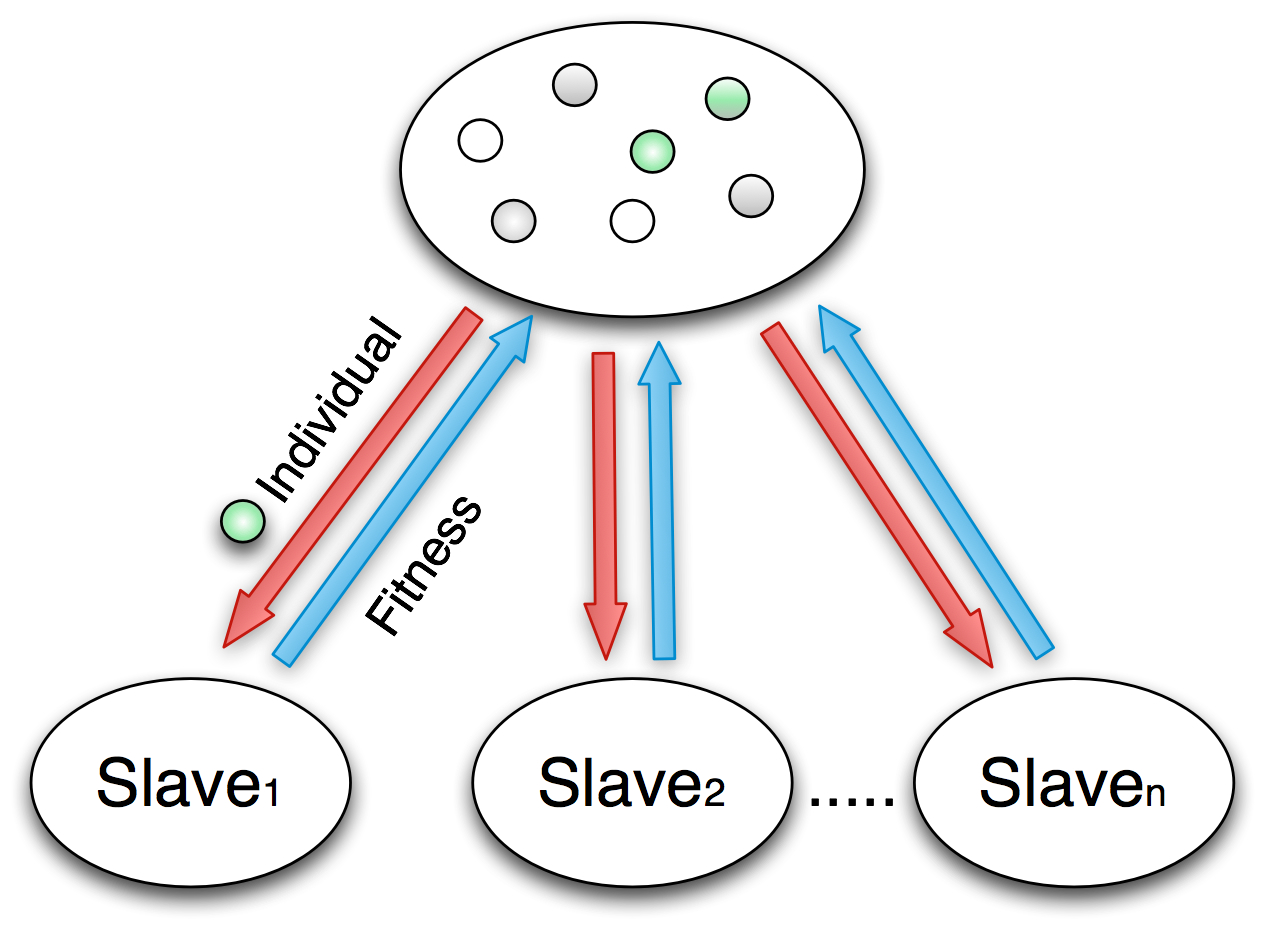
\includegraphics[width=20pc]{gfx/distributed/masterslave.jpg}
\caption{Master-slave model.}
\label{fig:masterslave}
\end{SCfigure}

\subsubsection{Spatially structured algorithms}
The parallelism is performed at population level, that is, dividing the population among the different computing elements. Depending on how the distribution is performed we have:
\begin{description}
\item[Coarse-grained approach] One of the most usual approaches is the \textsc{Island model}, where a number of nodes executes simultaneously the EA, working with different sub-populations at the same time. Each certain number of generations some individuals are interchanged (migrated) between populations. Figure \ref{fig:ring} shows this model with a ring topology.

\begin{SCfigure}[20][tb]
\centering
\includegraphics[width=20pc]{gfx/distributed/ring.jpg}
\caption{Island model scheme using a neighbourhood ring topology.}
\label{fig:ring}
\end{SCfigure}

\item[Fine-grained approach] In this approach, also called \textsc{Cellular EA} (CEA), each node has one individual of the population, and selection and reproduction are limited to the individuals of the neighbourhood of the node \cite{CELLULAR}. Usually a bi-dimensional grid is used as topology, such as the one showed in the Figure \ref{fig:cellular}.

\begin{SCfigure}[20][tb]
\centering
\includegraphics[width=5cm]{gfx/distributed/cellular.jpg}
\caption{Cellular Evolutionary Algorithm.}
\label{fig:cellular}
\end{SCfigure}

\end{description}

\subsection{New trends on parallel EAs} 
\label{chap:distributed:newtrendson}
% �Por qu� no convencionales?
                                % - JJ FERGU: Cambiado a new trends

When developing distributed and parallel EAs (or any distributed system in general), 
we should deal with the {\em Fallacies of Distributed Computing}, proposed by \person{Peter Deutsch}
and then explained by \person{Rotem-Gal-Oz} in \cite{rotem2006fallacies}.

\begin{enumerate}
\item The network is reliable.
\item Latency is zero.
\item Bandwidth is infinite.
\item The network is secure. 
\item Topology doesn't change. 
\item There is one administrator. 
\item Transport cost is zero. 
\item The network is homogeneous.
\end{enumerate}

These fallacies were not taken into account in the previous classification. %why? - JJ
 However, with the advent of new
technologies, such as cloud computing,
\definicion{P2P}{Peer-to-peer} networks, or the usage of heterogeneous
hardware, new approaches have been proposed. % that take into account, for instance, unreliability... jolines, explica las cosas bien - JJ 
 Distributed EAs can be
executed in other computing elements different than the classic
computers. For example, in mobile devices \cite{Garcia2009Mobile},
``smart dust'' \cite{Rollings2008smartdust} or inside robots, 
learning from the environment in an on-line manner \cite{Garcia2012testing}. But with
the advancement of the Internet, where millions of nodes can
co-operate, and whose behaviour is not totally controlled or
predicted, is when new distributed approaches have become more
evident.  

% �Esto es una clasificaci�n? �A qu� nivel est�s clasificando? �C�mo
% encaja esto dentro de lo que has escrito en los primeros p�rrafos?
% �Y de TU TESIS? - JJ FERGU: quitada la clasificaci�n
%\subsubsection{P2P evolutionary algorithms}

P2P systems are parallel infrastructures composed by a large number of
resources, % eso no define los sistemas P2P, sino sus
           % conexiones. Pueden tener 3 recursos. Adem�s, �qu� diablos
           % significa recurso en este contexto? - JJ
without any central server \cite{steinmetz2005peer}. In practice, the
resources in these networks can appear or disappear dynamically. These
platforms can be used to execute large instances of problems, taking
advantage of the massive scalability that these systems potentially
offer. %La escalabilidad no la da el sistema, sino el algoritmo. Algo
       %tan f�cil como una b�squeda puede colapsar la red si el
       %algoritmo no es el correcto. Mira esto: Loo, Boon Thau, et al. "Measurement and Analysis of Ultrapeer-based P2P Search Networks." (2003).
 An example of one EA that has been designed to take advantage of these systems, is
  \definicion{EvAg}{Evolvable Agent}, proposed by \person{Laredo \etal}�\cite{laredo2010evag}. This algorithm
  uses a decentralized population, where each peer has a single
 individual, and new individuals are created combining the ones in
 their current neighbours. % hala, non-sequitur. �Un ejemplo? �El m�s
                           % guay? �El m�s actual? �Soluciona qu�
                           % problemas y como? - JJ FERGU: un ejemplo, y el problema que resuelve, a�adido
To solve the problem of the dynamic topology, the population structure is maintained using the \textsc{newcast}
protocol \cite{jelasity2003newscast}: each node has a cache of
neighbours that can be interchanged and combined. Figure
\ref{fig:evag} shows this algorithm and its population
structure. Results show that this algorithm outperforms tuned GAs,
using less links that a panmictic (i.e. fully connected) population. 
% resolviendo el problema de conectividad fija (con DHT) o la introducci�n de nodos destacados (ultrapeers). Esto es un protocolo tipo gossip que podr�as mencionar y en todo caso el primer sistema P2P de EAs no fue este, sino DREAM, de donde desciende - JJ

\begin{SCfigure}[20][tb]
\centering
\includegraphics[width=26pc]{gfx/distributed/evag.jpg}
\caption{P2P Evolutionary Algorithm: EvAg.}
\label{fig:evag}
\end{SCfigure}

%\subsubsection{Pool-based algorithms}
Technologies such as non-relational databases % �cu�les? �Por d�nde? �C�mo? FERGU: est�n explicadas despu�s
lead to \textsc{Pool-based EAs} \cite{merelo2010fluid}, where the computational nodes
exchange individuals using a shared pool. 
Although this can be seen as a farming model, there are differences 
in how the data flow of individuals is managed.
% si son individuos para
                                % evaluar, se trata simplemente de
                                % "farming". Lo interesante es el
                                % flujo de datos de estos
                                % individuos. �Y cita nuestros papers
                                % y otros, como el de Gagn�! - JJ FERGU: A�adida tu cita (aunque m�s tarde cito todos)
This allows massive scalability with a heterogeneous underlying
structure. This pool can be used as the global population, and the
nodes asynchronously read and evaluate the individuals. It can also be used
to share individuals among islands. % una posibilidad... y otra
                      % posibilidad... clasificaci�n de tipo
                      % Borges. �Hay que ser exhaustivo y describir de
                      % qu� se trata este tipo de algoritmo! - JJ FERGU: reescrito
This can lead to automatic load-balancing and synchronization,
allowing the addition and removal of nodes. % s�
                                % consistente. "computer" "node"
                                % "individual". �No ibas a establecer
                                % la terminolog�a en este cap�tulo? - JJ FERGU: voy a usar "nodo" como elemento de c�mputo
Different technologies can be used. For example, in the work of
\person{Meri \etal},  the pool used is based on the
Dropbox\texttrademark\, or SugarSync\texttrademark\ file storage
services. Other authors propose the use of non-relational databases,
such as the work of \person{Merelo \etal} \cite{merelo2010fluid},
using FluidDB\texttrademark. In \cite{merelo2012pool} the same authors
improve the design, proposing an asynchronous, fault-tolerant, and
scalable dEA, based on the object store CouchDB\texttrademark. The
results show that adding clients could not scale, but increase the
fault tolerance. Also, their experimentation shows a good methodology
for designing EAs in heterogeneous distributed systems, which have the
impossibility of analytic performance prediction. 

%\subsubsection{Grid and volunteer computing} %Clasificaci�n tipo
                                %Borges. la computaci�n voluntaria
                                %puede ser "cl�sica", "basada en pool"
                                %o incluso P2P (dependiendo del
                                %cliente). FERGU: quitada clasificaci�n
Other systems, such as Grids \cite{grid1} are distributed computing systems that allow sharing
geographically distributed resources to solve large scale
problems. % grid es el predecesor de la computaci�n nube. Tampoco
          % tiene mucho que ver con la computaci�n voluntaria, salvo
          % que se le llama "desktop grid". Sep�ralos (y justifica
          % bien la clasicaci�n real). - JJ
Several works that describe EAs being executed
% no uses "There exist" como en el chiste de Gila "Hay alguien que ha
% hecho algo malo..." - JJ FERGU: Cambiado 
in these systems have been presented \citep{grid8,grid4,grid10}. \textsc{Volunteer
  computing} \cite{anderson2005high} proposes the creation of
infrastructures to allow people donate CPU cycles for a combined
computational effort. Its main difference with grid computing is the
presence of un-trusted resources: for example, some nodes could return
intentionally wrong results, so it requires the possibility of
replication of the results to be validated. % �posibilidad de replicaci�n? - JJ FERGU: arreglado
Also, the control of the participating nodes is not
maintained by the experiment launcher. EAs have been executed in these
systems, using several techniques, such as virtualization
\cite{Fernandez2013BOINC} or ``parasite'' computing
\cite{Merelo2007browser}. % Esta no es par�sita, los participantes
                          % estaban avisados - JJ

Summarizing, with these new trends in parallel EAs, researchers must deal 
with heterogeneous hardware and different communication protocols, but also
 with dynamic, non-centralized or uncontrolled environments. %FERGU: ...enlazando con la tesis...

 


\section{Parameter adaptation in Evolutionary Algorithms}
\label{chap:distributed:parameteradapt}
% y esto viene a cuento porque... - JJ

\lettrine{O}{ne} of the greater challenges of the EC field is to find
the appropriate values for EAs parameters
\cite{Eiben12Parameters}. Usually, these parameters are established by
convention or after several test runs, for example. However,
practitioners need to put effort on finding these values in order to
attain significant performance in their EAs, even taking into account
other variables, such as the computational power of the machines
used.

\subsection{Parameter Control and Parameter Tuning}
\label{chap:distributed:pcontroltuning}
There are two different approaches for algorithm parameter setting  in EC: {\em parameter control} and {\em parameter tuning} \cite{ParameterControlEiben99}. The first one refers to setting up a number of parameters for the Evolutionary Algorithm (EA) and changing them in running time. The parameter tuning consists in establishing a good set of parameters {\em before} the run (and not changing these parameters during runtime).

\person{Eiben}, in \cite{ParameterControlEiben07} proposes the next taxonomy for the parameter control, according to {\em how} the are changes made:
\begin{itemize}
\item Deterministic methods: changes to a parameter are triggered by a deterministic rule (for example, increase mutation rate after certain number of generations).
\item Adaptive methods: parameters change depending on some behaviour (for example, increase mutation rate if the average fitness of the population stagnates).
\item Self-adaptive methods: parameters are encoded within the chromosome of the individuals of the population (for example, mutation rate can be a value in the chromosome).
\end{itemize}

Other classifications for control techniques in EAs are presented in that work. For example, regarding to {\em what} is changed:
\begin{itemize}
\item Representation
\item Evaluation function
\item Variation of operators and their rates
\item Selection operators
\item Replacement operator
\item Population
\end{itemize}

Finally, a third classification can be obtained according to what evidence is available:
\begin{itemize}
\item Absolute evidence: The parameter changes if a rule is activated when an specific event occurs. For example: increase mutation rate when diversity drops. In this case, human knowledge is necessary to model these rules.
\item Relative evidence: Parameters are compared with the fitness of their produced offspring and the best values are rewarded. It is not deterministic.
\end{itemize}

These classifications can be used to establish a way to manage or update the parameters 
in the development of algorithms. For example, it should be necessary to allow a direct
 access to each parameter and sources of information of the EA, independently of the actual 
 state of the algorithm. A possible solution to manage 
the dynamic parameters, and the information of the elements that conform the EA, is proposed in next chapters.
% Vale, llego aqu� y todav�a no s� qu� diablos tiene que ver con los
% SOA y el OSGi y OSGILIATH - JJ FERGU: estoy cambiando este cap�tulo para indicar los problemas en desarrollo, integraci�n, estandarizaci�n y dinamismo en EAs. Luego dir� "necesitamos una soluci�n para esto!" (y a�adido el p�rrafo de arriba)

\subsection{Adaptation in heterogeneous hardware}
\label{subsec:distributed:adapthetero}
Adapting algorithm parameters to available computational resources
leads to improved performance (see the work of \person{Hamadi and
  Schoenauer} \cite{AutomaticallyConfiguringStyles12}). An easy way to
take advantage of the available resources is  balancing the workload
\cite{Garamendi2006Parallel} to distribute it across multiple
nodes. % �elements, computers, individuals, nodes? - JJ fERGU: cambiado a nodos
However, assigning the same tasks to each node on heterogeneous
clusters may result in suboptimal performance (as shown by
\person{Bohn and Lamont} \cite{LoadBalancingBohn02}). Parameters of an
algorithm could also be adapted to increase the performance of the
whole system. For example, the population size in EAs is the key to
obtain good performance, because it has % �Gram�tica! - JJ FERGU: qu� error hay? (lo has corregido, no?)
 effect on the quality of the solution and the time spent during the run \cite{ShrinkageLaredo09}. This parameter has been studied as a fixed \cite{SizingHarik99} or adaptive parameter during runtime \cite{AdaptiveLobo07,SelfRegulatedSizeFernandes06}, but without taking into account the computational power of each machine in a heterogeneous cluster. 

The adaptation of an algorithm can be useful to leverage different hardware environments.
One of the problems in parameter adaptation in heterogeneous clusters is 
the representation of the computational load. It depends on the algorithm, size of the problem, programming 
language, compiler or hardware characteristics, and the results obtained from artificial 
benchmarks (such as  Linpack \cite{LinpackEndo10}) should not be extolled as identificative 
of the system performance \cite{LinpackDongarra03}. For example, in the work of \person{Garamendi 
\etal} \cite{Garamendi2006Parallel},  a small benchmark was executed in all nodes at the beginning
of the algorithm in order to distribute individuals of an Evolutionary
Strategy, following a master-slave model. % but... - JJ FERGU: es lo siguiente (lo enlazo con However)
However, the computational load by artificial benchmarks may not accurately 
 represent the correct load of the algorithm, so, information 
 about the algorithm itself should be used for calibration. % sez who? FERGU: TODO buscar la referencia que encontr�!
                                % �Esto es tu tesis? - JJ FERGU: esto es para la parte de homoheterosize, lo pongo aqu� o all�?

In other works, there is no direct relation between the algorithm parameters and 
computational resources of the nodes. % sez who again? - JJ
For example, \person{Dom\'inguez \etal} \cite{Dominguez13HydroCM} 
divided the available devices into ``faster'' and ``slower'' nodes to create a distributed hybrid 
meta-heuristic that combines two different EAs: Genetic Algorithms and Simulated
Annealing. Their system executes the heavy (in computational
terms) algorithms (GAs) in the faster nodes (computational devices), and
simpler meta-heuristics (SA) in the slower ones, obtaining better results
than other configurations.  \person{Gong \etal} in \cite{Gong2005HeterogeneousTopology} also ordered 
the nodes by their computational power to test different topology configurations in a distributed EA.
Besides,  ordering the nodes taking into account 
only their previously known computational resources, the results of the previous works were not compared with executions on a homogeneous 
cluster to validate if the adaptation takes advantage of the heterogeneity 
of the cluster.

The heterogeneous computational performance of nodes or network speed can affect the performance of an algorithm. In \cite{Alba2002Heterogeneous},
 \person{Alba \etal} compared a distributed Genetic Algorithm (dGA), one of
 the sub-types of EAs, on homogeneous and heterogeneous clusters. 
 Super-linear performance in terms of iterations was obtained in the heterogeneous ones,
 being more efficient than the same algorithm running on homogeneous
 machines. However, the parameter setting was the same in both
 clusters and they did not adapt the parameters to the machines used.

 Adapting algorithm parameters to different nodes % ahora
                                % computational nodes - JJ FERGU: todo va a ser nodes ahora (cambiado a different)
derives in heterogeneous parameter sets. These sets can improve the results in homogeneous hardware, for example, setting a random set of parameters in each homogeneous node can also increase the
performance of a distributed Genetic Algorithm, as explained by \person{Gong
and Fukunaga} in \cite{Gong2011HeterogeneousParameters}. That model
outperformed a tuned canonical dGA with the same parameter values in
all islands. Also, adapting the migration rate produced better
results than homogeneous periods, as explained by \person{Salto and Alba} in
\cite{Salto2012HeterogeneousMigration}. This indicates that heterogeneous parameters
 may lead to an increase of performance, so it is necessary to validate if the 
 performance is due to the parameter set or to the heterogeneous
 devices combination. The way to access  the elements that conform 
 an EA (including their parameters) proposed in this thesis will be used 
 in next chapters to address this issue.


 % que es lo que vamos a hacer en esta tesis. O
                      % as�. - JJ FERGU: puesto �est� bien?


\section{Development of Evolutionary Algorithms} %FERGU: Cambiado t�tulo de la secci�n
\lettrine{O}{ne} of the aims of this thesis is to facilitate the standardization, 
integration and development of EAs.
% Y esto viene a cuento porque... la "narrativa" de este cap�tulo
% tienes que hacerla al principio del mismo, integrarlo todo en TU
% TESIS a la vez que estableces el estado del arte - JJ FERGU: a�adido arriba

 % cada vez que dices There exist, $deity mata a un gatito - JJ FERGU: Okis, los quito todos
This is due to the existing large number of frameworks for Evolutionary
Algorithms. 
Practically every programming language has its own implementation of the basic elements
that form an EA. This implies a large effort made in each one, giving
that these elements are not compatible among them. It is also
difficult to migrate the code from a framework to another, mainly due
to design choices, such as the existence of hidden global variables or
language specific features (such as functional programming
\cite{Cruz2013Erlang}). This is important for example, to integrate and reuse 
the elements of the frameworks in other systems (such as enterprise servers, for example). 
However, is in the field of Open Science \cite{Altunay2011OpenScience} where the integration and standardization of
the elements that conform an EA can take advantage, facilitating the re-use and access 
to existing software, systems, data, and results.
%FERGU: DONE
 % Y migrar c�digo es importante porque... - JJ

% di lo que es importante: genericidad, comunicaci�n,
% prestaciones... Y eval�a cada framework con respecto a esto para
% finalmente decir que tu framework va a ser mejor, pero recuerda que
% tu tesis no es tu framework - JJ

In this section, the genericity, communication and features of the 
development of EAs and existing frameworks are explained and compared 
to evaluate their benefits and shortcomings. 

\subsection{Design of EAs}
\label{sec:distributed:design}
The work of \person{Gagn\'e and Parizeau} \cite{GENERICITY05} established six criteria to qualify the genericity of a framework for EAs. 

\begin{itemize}
% resalta algo, hombre - JJ FERGU: hecho
\item {\em Generic representation}: independence of the structure of the individuals. 

\item {\em Generic fitness}: Individual fitness should be as independent as possible from the selection operators and individual representation. That means that the fitness evaluation should be outside of the implementation of the individuals (for example, not implementing the fitness in the class that implements the individual). 

\item {\em Generic operations}: operations should be used in conjunction with others and have minimal side effects. For example, a multi-parent reproduction (crossover with more than two parents, as presented by \person{Eiben et al.} \cite{EibenMultiparent97}) requires separation of the concept crossover with only two elements, so the abstract concept of crossover  should accept a list of individuals. Also, new operations can be created without affect the existing ones, allowing the interaction of a non-limited number of operators. Finally, the granularity of the design of the operators should be equilibrated, not being neither too coarse (may limit the flexibility to create new operators) nor too fine (could be difficult to integrate all the operators).

\item {\em Generic evolutionary model}: As explained in Section \ref{subsec:classicEAs}, % �d�nde? - JJ FERGU: hecho
there exist different ways to model an EA leading to different algorithms (for example, a steady-state GA versus a generational GA, or a GA versus ES). Operators should be independent of the evolutionary model, being possible the change from a model to another. 

\item {\em Parameter management}: parameters, such as the population size, may be modified during runtime. Also, a good framework should accept the addition of new parameters.

\item {\em Configurable output}: the output should be configurable. This is due to different statistics that could be used depending on the EA: for example, the tree depth in GP. Also, different outputs (console, files) should be managed.

\end{itemize}

 These issues should be accomplished to develop new algorithms or operators, with independence of the programming language used. However, as will be explained in next chapters, new models of design and development can extend the previous criteria.

\subsection{Frameworks for EAs}
\label{subsec:soaea:fworks}
Over the large number of available frameworks (see \cite{SURVEYMOFS} for a complete survey) a representation of them has been selected to explain their shortcomings, that will be addressed in this thesis.

 % se est� quedando sin gatitos - JJ FERGU: Quitado el There exist
Object Oriented programming is used in several frameworks, such as Al\-go\-rithm::Evo\-lu\-tionary \cite{PERL}, \definicion{METCO}{Metaheuristic-based Extensible Tool for Collaborative Optimization} \cite{Leon2009metco},
\definicion{JCLEC}{Java Class Library for Evolutionary Computation} \cite{JCLEC} or jMetal \cite{JMETAL}. 
 Users implement specific interfaces of these frameworks ({\em
   individual} or {\em crossover}, for example) and they group them in the source
 code. For example, creating an operator object that groups several
 operators. However, these frameworks are not compatible among them.
 For example, the operators created in JCLEC can not be used directly in jMetal
 (despite both are programmed in Java). %Also, they can not control the
 %services (operators) outside the source code.

%\subsection{Parallel frameworks} % y Borges sin
                                % animales. Algorithm::Evolutionary
                                % puede ser paralelo los paralelos
                                % orientados a objetos - JJ FERGU: quitadas todas las subsecciones
Parallelism and distribution are possible in other frameworks, such as
MALLBA \citep{MALLBA}, \definicion{DREAM}{Distributed Resource
  Evolutionary Algorithm Machine} \citep{DREAM} or
\definicion{ECJ}{Evolutionary Computation in Java} \citep{ECJ}, but 
using external libraries (such as \definicion{MPI}{Message Passing Interface} or \definicion{DRM}{Distributed Resource Machine}), so the code that uses these
libraries is mixed with the algorithm's code.


 Even being distributed, these frameworks can not communicate with
 each other. This implies an extra effort to combine the capabilities 
 that a framework can offer to other frameworks or other programs (for example, a web server). %lo que es un problema por... - JJ FERGU: puesto
  HeuristicLab \citep{HEURISTICLAB} is one of the few plug-in and service oriented frameworks. It uses web services for communication, but only to distribute the load, after consulting a central database of available jobs. Finally, %the only service oriented optimization framework is
 gridUFO is a service oriented framework \citep{gridUFO}, but it only allows the modification of the objective function and the addition of whole algorithms, without combining existing services.  Table \ref{tab:frameworks} shows a summary of the previous frameworks.


\begin{SCtable}[][t]
\resizebox{11cm}{!}{
\begin{tabular}{llllll}
\hline
\rowcolor{colorCorporativoSuave}Name		&  Design 	 & Language 	& Distribution 	& License  		& Last version	\\
\hline\hline
\rowcolor{colorCorporativoMasSuave}ECJ		& OO		& Java		& Sockets   	& Academic Free Lic. 	& 2013		\\
\rowcolor{colorCorporativoSuave}MALLBA		& OO		& C++		& MPI		& Freeware		& 2010	\\
\rowcolor{colorCorporativoMasSuave}jMetal		& OO		& Java		& N/A		& GNU/LGPL 		&2013		\\
\rowcolor{colorCorporativoSuave}DREAM		& OO		& Java		& DRM		& GNU/GPL   		& 2003		\\
\rowcolor{colorCorporativoMasSuave}ParadiseEO	& OO		& C++		& MPI		& CeCILL	   	& 2012		\\
\rowcolor{colorCorporativoSuave}HeuristicLab	& OO/PO 	& .NET		& Web-Services	& GNU/GPL		& 2013			\\
\rowcolor{colorCorporativoMasSuave}METCO		& OO		& C++		& MPI		& N/A	   		& 2009	\\
\rowcolor{colorCorporativoSuave}JCLEC		& OO		& Java		& N/A		& GNU/GL   		&	2013 \\
\rowcolor{colorCorporativoMasSuave}Algorithm::Evol.& OO		& Perl		& N/A		& GNU/GPL  		& 2013	\\
\rowcolor{colorCorporativoSuave}gridUFO		&SO		& Java		& Web Services	& N/A  			& 	2010 \\
\hline
%OSGiLiath	&OO/SO/PO 	& 2010			& Java		& Distributed OSGi	& GNU/GPL  	& Lifecycle management	\\
\end{tabular}
}
\caption{Comparison of EA frameworks. OO=Object-Oriented, SO=Service Oriented, PO=Plug-in Oriented}
\label{tab:frameworks}
\end{SCtable}
% qu� pasa con DEAP? - JJ http://code.google.com/p/deap/ �Seguro que
% no hay m�s? FERGU: s�, hay m�s (a�ado un survey) pero digo al principio que hemos hecho una selecci�n

In brief, although these frameworks follow the six criteria for genericity 
proposed by \person{Gagn{\'e} and Parizeau} previously explained, they present some shortcomings when it is needed to develop
or add new features: the user is forced to modify the source code
or stop the execution to add new functionalities (like load balancing,
dynamic control of operators, or an user interface).


%\subsection{Volunteer computing frameworks} FERGU: enlazado con lo anterior
Other frameworks, not focused on EAs, can be used to deal with some of the issues, such as dynamism in nodes. \definicion{BOINC}{Berkeley Open Infrastructure for Network Computing} is one of the most used frameworks in volunteer computing. This middleware follows a master-slave architecture, where the server is in charge of hosting the project experiments and the creation and distribution of jobs \cite{Fernandez2013BOINC}. Clients ask the server for works, download information, compute data and upload the results. EAs have been used in BOINC, such as the work of \person{Fern\'andez \etal} \cite{Fernandez2013BOINC}. Other authors imitate this architecture using a browser-based scheme \cite{Merelo2007browser} to distribute fitness evaluations among clients without installing any other software. Previous systems have the possibility of task distribution among the nodes, following a master-slave model, but without interaction between clients. Also, these systems does not count with automatic discovering of operators.



% �Y ah� se queda? Una tesis no puede ser "te cuento todo esto a
% cascoporro y ya m�s adelante si eso te contar� por qu� te lo he
% contado". Una tesis es "te voy a contar esto, te estoy contando esto
% porque te voy a contar lo otro, te estoy contando lo otro porque te
% he contado esto, y te he contado esto y lo otro". -JJ FERGU: reescribiendo todo. Es que hab�a pensado hacerlo en plan "Hay muchos problemas, hay estas tecnolog�as, voy a usarlas para resolverlos" sin dar pistas de c�mo (y sin enlazar entre s�). Como ver�s estoy poniendo mucho "the aim of this thesis is..." y. FERGU: TODO

\section {Conclusions}
\label{chap:distributed:conclusiones}

\lettrine{E}{volutionary} Algorithms, and their subtypes (GAs, ES or GP, among others) follow a number of common steps: initialization, evaluation, selection, recombination, mutation, replacement and stop criterion. There exist many variations of these steps, and the different combinations can specify one algorithm or another. Memetic Algorithms also include extra elements that can be applied, and different heuristics can be combined during the algorithm's run.

Distributed EAs can improve the algorithmic and computational
performance over the non-parallel versions of the algorithms. % over what? - JJ FERGU: non-parallel versions est� bien?
 Classic parallelization approaches, such as the master-slave or island-based models, have been updated with the usage of new trends such as P2P or pool-based EAs. These new approaches manage with computational nodes entering and exiting during the experiment runtime and heterogeneous architectures.

Other research lines, such as the parameter adaptation can imply the existence of some kind of dynamism involving the parts that compose an algorithm: for example, different recombinators or mutators working at the same time. Moreover, there exist several lines of parameter adaptation in dynamic and heterogeneous environments, where different computational elements are working at the same time.

Finally, there exist a large number of different (and incompatible) frameworks for EAs, each one using different languages, technologies and communication protocols. As \person{Parejo \etal}  suggest  in \cite{SURVEYMOFS}, a standardization of the presented (and other) frameworks should be carried out. Moreover, it is difficult to access, in a public way, to available public systems to execute existing EAs to validate experiments and save time, encouraging Open Science.

% y todo esto es interesante para mi tesis porque... �No la has
% mencionado ni una vez! - JJ FERGU: Cambiado lo anterior y lo siguiente

Next chapter will explain a possible technological solution to cope with the 
previous issues that will be addressed in this thesis: development, integration, standardization and dynamism in EAs. % which ones? Which ones are your thesis? - JJ FERGU: puestas}{\myChapter{Evolutionary Algorithms}\label{chap:distributedEAs}}
%\ifthenelse{\equal{\value{IncluyeCapitulo}}{5}}{\myChapter{Cuestionarios sobre \textsc{Baja Visi�n}}\label{sec:cuestionariosBajaVision}
\minitoc\mtcskip
\vfill
\lettrine{P}{uesto} que uno de los �mbitos de actuaci�n de esta Tesis es el de los pacientes con \textsc{Baja Visi�n}, a continuaci�n se expone un estudio en el que se muestra qu� aspectos se contemplan en los cuestionarios de evaluaci�n de los pacientes de \textsc{Baja Visi�n}. Este cap�tulo se basa en la revisi�n cient�fica de diversos cuestionarios de evaluaci�n de la funci�n visual de pacientes con \textsc{Baja Visi�n} realizada por \person{Massof \etal} \citep{massof01}. La mayor�a de estos cuestionarios se dise�aron para detectar la \textsc{Baja Visi�n} en pacientes, y ninguno trata de medir el grado de acomodaci�n de estos pacientes a im�genes procesadas. Todos los cuestionarios estudiados en dicho art�culo son de tipo \emph{ling\"{u}�stico}, mientras que los que se necesitan para la evaluaci�n de los algoritmos de procesamiento de contornos, que se utilizar�n a lo largo de esta Tesis, han de ser de tipo visual. Sin embargo, aunque la revisi�n de estos cuestionarios no garantizar� la \textsc{validez} del cuestionario de evaluaci�n de calidad de bordes, puede servir como un buen punto de inicio para el desarrollo de dicho cuestionario, sobre todo para escoger los grupos de im�genes que se utilizar�n para su procesamiento.
\clearpage
\section{Investigaci�n sobre la \textsc{Baja Visi�n} mediante cuestionarios}
\lettrine{E}{xisten} algunos estudios que eval�an tanto la funci�n visual de los pacientes que sufren \textsc{Baja Visi�n} como la influencia de su patolog�a en otros aspectos de su vida habitual. \person{Massof \etal} \citep{massof01} realizaron un art�culo en el que se hizo una revisi�n cient�fica muy exhaustiva de muchos cuestionarios de evaluaci�n de la funci�n visual de pacientes con \textsc{Baja Visi�n}. Tomando como base dicho trabajo, a continuaci�n, se realizar� una exposici�n de los principales cuestionarios para pacientes con \textsc{Baja Visi�n}, haciendo especial hincapi� en la descripci�n de los \textsc{dominios} de cada cuestionario. Se ha optado por indicar el nombre de cada cuestionario en el idioma original sin traducirlo al espa�ol, ya que muchos de estos cuestionarios est�n ampliamente difundidos con los nombres originales y la traducci�n de los mismos podr�a llevar a problemas de identificaci�n y dificultar su localizaci�n en otros textos cient�ficos.
\subsection{Visual Function Index}
Desarrollado por \person{Bernth--Petersen} \citep{bernth81}, el cuestionario \definicion{VFI}{\textsc{Visual
Function Index}, �ndice de Funci�n Visual.} est� dividido en 9
\textsc{items}, que cada uno podr�a identificarse, a su vez, con un \textsc{dominio}. Cada pregunta tiene una graduaci�n diferente de posibles respuestas:
\begin{enumerate}
\item Lectura (\emph{Nada, S�lo letras grandes, Letras peque�as}).
\item Visi�n a media/larga distancia (\emph{Buena, Moderada, Pobre}).
\item Ver la Televisi�n (\emph{S�, No}).
\item Conducci�n de autom�vil/bicicleta (\emph{S�, No}).
\item Orientaci�n en interiores (\emph{S�, No}).
\item Orientaci�n en exteriores (\emph{S�, No}).
\item Actividad ``principal'': trabajo, tareas del hogar (\emph{S�, No}).
\item Otras actividades: ocio, ir de compras, etc. (\emph{S�, No}).
\item Actividades de ``cuidado personal'': comer, aseo, ba�arse, etc. (\emph{S�, No}).
\end{enumerate}
\clearpage
\subsection{Rand Questionnaire to Assess Functional Problems of the Visually Impaired}
\person{Bikson} y \person{Bikson} \citep{bikson81}, de la empresa \person{Rand Corp.}, dise�aron el
cuestionario \definicion{Rand--FPVI}{\textsc{Rand questionnaire to assess Functional Problems of the Visually
Impaired}, Cuestionario Rand para determinar los Problemas Funcionales de los Deficientes Visuales.}, compuesto por 30 \textsc{items} agrupados en 8 \textsc{dimensiones}:
\begin{enumerate}
\item Habilidades para la vida independiente.
\item Orientaci�n general.
\item Movilidad general.
\item Viajar en autob�s.
\item Problemas de iluminaci�n.
\item Tareas del hogar.
\item Percepci�n social.
\item Actividades recreativas.
\end{enumerate}
\noindent En todos los casos, las preguntas tienen 3 posibles respuestas: \emph{Sin afectaci�n, Afectado por
sus problemas de visi�n, Afectado por otros problemas distintos a los de su visi�n}.

\subsection{Visual Function after Pan--Retinal Photocoagulation}
El cuestionario \definicion{VF--PRP}{\textsc{Visual Function after Pan--Retinal Photocoagulation}, Funci�n Visual tras Fotocoagulaci�n Pan--Retinal.} fue desarrollado inicialmente por \person{Russell \etal} \citep{russell85} y posteriormente fue refinado por \person{Kosnik \etal} \citep{kosnik88}.\\
\noindent Este cuestionario consta de 27 \textsc{items} que se dividen en 8 \textsc{dominios}:
\begin{enumerate}
\item Velocidad de procesamiento visual.
\item Sensibilidad a la luz.
\item Visi�n a distancia.
\item Visi�n cercana.
\item Visi�n binocular.
\item Visi�n nocturna.
\item Falta de fluidez visual.
\item Adaptaci�n a la luz.
\end{enumerate}
\noindent En todos los casos, los \textsc{items} presentan a los pacientes respuestas en las que se mide
cu�ndo han tenido dificultad al realizar una determinada tarea en relaci�n con la fotocoagulaci�n
pandiab�tica: \emph{Nunca, Antes, Justo despu�s, Ahora}. En caso de responder \emph{Ahora}, se a�ade una segunda escala en la que se cataloga el grado de la dificultad: \emph{Suave, Moderada, Severa, Intolerable}.

\subsection{Visual Status Inventory}
\person{Coren} y \person{Hakstian} dise�aron y validaron el cuestionario \definicion{VSI}{\textsc{Visual
Status Inventory}, Inventario de Estado Visual.} \citep{coren87} con 52 \textsc{items} para la estimaci�n de la discapacidad visual en estudios epidemiol�gicos. Estos \textsc{items} se distribuyen en tres \textsc{dominios}:
\begin{enumerate}
\item Agudeza visual.
\item Visi�n en color.
\item Funci�n binocular general.
\end{enumerate}
\noindent Las respuestas pretenden medir la frecuencia con la que los pacientes son capaces de realizar una
actividad. \'{E}stas est�n estructuradas utilizando una escala de Lickert de 5 puntos, que cubre desde
\emph{Nunca} hasta \emph{Siempre}.
\subsection{Lowe's Visual Function}
\person{Lowe} desarroll� un cuestionario, denominado gen�ricamente \definicion{LVF}{\textsc{Lowe's Visual Function}, Funci�n Visual de Lowe.}, que posteriormente fue refinado por \person{Elliott \etal} \citep{elliott90}, para la medici�n de la funci�n visual para pacientes con cataratas en, al menos, un ojo.\\
\noindent Este cuestionario est� compuesto por 14 \textsc{items} agrupados en 4 \textsc{dominios}:
\begin{enumerate}
\item Movilidad: Caminar por el exterior, cruzar la calle, conducir, etc.
\item Visi�n cercana: Lectura de libros, lectura de peri�dicos, etc.
\item Discriminaci�n: Reconocimiento de amigos, lectura del n�mero de autob�s, ver la televisi�n, etc.
\item Calidad de visi�n: Visi�n con el ojo derecho, visi�n con el ojo izquierdo, visi�n binocular.
\end{enumerate}
\noindent Las respuestas se presentan como una escala continua de 10 cm. en la que los pacientes deben
situar una marca en la que se identifica el grado de discapacidad que sufren ante cada \textsc{item}.
\subsection{Questionnaire for Functional Assessment of Low Vision}
\person{Szlyk \etal} \citep{szlyk90} dise�aron un cuestionario para catalogar de manera funcional el grado de \textsc{Baja Visi�n} de los pacientes. Este cuestionario, llamado \definicion{FALV}{\textsc{questionnaire for Functional Assessment of Low Vision}, Cuestionario para Determinaci�n Funcional de la \textsc{Baja Visi�n}.}, est� basado en el trabajo de \person{Coren} y \person{Hakstian} \citep{coren87} (dise�adores del cuestionario \textsc{VSI}), y en el de \person{Kosnik \etal} \citep{kosnik88} (refinaron el cuestionario \textsc{VF--PRP}). Este cuestionario se ha implementado teniendo en cuenta \textsc{dominios} funcionales que pudieran ser evaluados tambi�n por los instructores de rehabilitaci�n de los pacientes, simplemente observando el comportamiento de los mismos.\\
\noindent Este cuestionario est� compuesto por 57 \textsc{items} agrupados en 4 \textsc{dominios}:
\begin{enumerate}
\item B�squeda (\emph{Cerca, Cerca por debajo, Cerca por encima, Lejos}).
\item Detecci�n (\emph{Cerca, Cerca por debajo, Cerca por encima, Cerca a la izquierda, Cerca a la derecha, Lejos}).
\item An�lisis (\emph{S�, No}).
\item Seguimiento (\emph{S�, No}).
\end{enumerate}

\subsection{Visual Activities Questionnaire}
Los pacientes de la $3^a$ edad suelen presentar una disminuci�n de la calidad visual, y \person{Sloane \etal} \citep{sloane92} quisieron medir dicho nivel de calidad visual de manera indirecta, a trav�s de la capacidad de los pacientes para realizar actividades cotidianas. Esta medici�n se realiz� mediante un cuestionario denominado \definicion{VAQ}{\textsc{Visual Activities Questionnaire}, Cuestionario de Actividades Visuales.}.\\
\noindent Este cuestionario est� compuesto por 33 \textsc{items} agrupados en 8 \textsc{dominios}:
\begin{enumerate}
\item Visi�n perif�rica.
\item Agudeza visual.
\item B�squeda visual.
\item Profundidad.
\item Color.
\item Adaptaci�n.
\item Deslumbramientos.
\item Velocidad de procesamiento visual.
\end{enumerate}
\noindent Las respuestas a los \textsc{items} representan la frecuencia en la que se le presenta cada
problema visual y se selecciona la alternativa mediante una escala de Lickert de 5 niveles, que va desde el ``\emph{Nunca}'' hasta el ``\emph{Siempre}''.

\subsection{Visual Performance Questionnaire}
\person{Bergman} y \person{Sj\"{o}strand} \citep{bergman92} crearon el cuestionario \definicion{VPQ}{\textsc{Visual Performance Questionnaire}, Cuestionario sobre el Rendimiento Visual.} para medir la prevalencia de la discapacidad visual en los ancianos.\\
\noindent Los autores no consideraron la agrupaci�n de los \textsc{items} en \textsc{dominios}, consistiendo
este cuestionario en 6 \textsc{items} �nicamente:

\begin{enumerate}
\item Ver la televisi�n.
\item Caminar por el exterior.
\item Lectura de libros y peri�dicos.
\item Lectura del list�n telef�nico.
\item Disfrutar de un hobby.
\item Realizar tareas del hogar.
\end{enumerate}
\noindent Las respuestas admisibles son dicot�micas y miden la capacidad de realizaci�n de cada tarea por parte de los pacientes.

\subsection{Activities of Daily Vision Scale}
La evaluaci�n de la funci�n visual mediante el cuestionario \definicion{ADVS}{\textsc{Activities of Daily Vision Scale}, Escala de Visi�n de Actividades Diarias.} fue desarrollada por \person{Mangione \etal} \citep{mangione92}.\\
\noindent Este cuestionario consta de 22 \textsc{items} agrupados en 5 \textsc{dominios}:

\begin{enumerate}
\item Visi�n a distancia (excluyendo la conducci�n).
\item Visi�n cercana.
\item Deslumbramiento.
\item Conducci�n diurna.
\item Conducci�n nocturna.
\end{enumerate}
\noindent En las respuestas se solicita graduar la dificultad que le requiere a los pacientes la realizaci�n de cada una de las actividades indicadas en los \textsc{items}. Esta graduaci�n se realiza utilizando una escala de
Lickert de 5 niveles, que va desde ``\emph{Sin dificultad}'' hasta ``\emph{He dejado de hacerlo debido a la
visi�n}''. Posteriormente, se a�adi� una $6^a$ opci�n en la que se indica que el paciente ha dejado de hacer la actividad (o no lo ha hecho nunca) por causas distintas a los problemas de visi�n.

\subsection{Assessment of Visual Function-Related Quality of Life}
Para medir tanto la funci�n visual como la calidad de vida de los pacientes, \person{Brenner \etal} \citep{brenner93} desarrollaron el cuestionario \definicion{VF--QOL}{\textsc{Visual Function--related Quality of Life}, Calidad de Vida relativa a la Funci�n Visual.}.\\
\noindent Este cuestionario consiste en 8 \textsc{items}:

\begin{enumerate}
\item Leer peri�dicos.\label{vfqol:1}
\item Leer el list�n telef�nico.\label{vfqol:2}
\item Leer etiquetas.\label{vfqol:3}
\item Leer precios.\label{vfqol:4}
\item Reconocer personas.\label{vfqol:5}
\item Ver los escalones.\label{vfqol:6}
\item Ver grietas en el pavimento.\label{vfqol:7}
\item Ver se�ales de tr�fico.\label{vfqol:8}
\end{enumerate}
\noindent A pesar de que los autores originales no los agruparon en \textsc{dominios}, \person{Massof \etal}
\citep{massof01} determinaron, utilizando an�lisis factorial, que los \textsc{items} pueden agruparse en 3
\textsc{dominios}:
\begin{enumerate}
\item Visi�n cercana (\textsc{items} \ref{vfqol:1} al \ref{vfqol:4}).
\item Visi�n de media distancia (\textsc{items} \ref{vfqol:5}, \ref{vfqol:6} y \ref{vfqol:7}).
\item Visi�n lejana (\textsc{item} \ref{vfqol:8}).
\end{enumerate}
\noindent Las respuestas a los \textsc{items} miden la frecuencia con que los pacientes han sentido alguna vez que su visi�n ha significado un problema para realizar cada \textsc{item}. Cada respuesta tiene 3 posibles
opciones: \emph{Nunca, A veces, Siempre}.

\subsection{14--Item Visual Functioning Index}
Dise�ado por \person{Steinberg \etal} \citep{steinberg94} para medir la funci�n visual de pacientes con cataratas, el cuestionario \definicion{VF--14}{\textsc{Visual Functioning index with 14--Item}, �ndice de Funci�n Visual utilizando 14 \textsc{�tems}.} requiri� un esfuerzo importante, que involucr� a muchos expertos de diversas disciplinas (desde oftalm�logos hasta estad�sticos, pasando por �pticos y otros m�dicos especialistas) y tambi�n a gran cantidad de pacientes con cataratas (tanto antes como despu�s de la operaci�n de cataratas).\\
\noindent Este cuestionario est� dise�ado con 14 \textsc{items}:

\begin{enumerate}
\item Lectura de peque�as impresiones (etiquetas, etc.)
\item Lectura de libros o peri�dicos.
\item Lectura de libros o peri�dicos con letras de gran tama�o.
\item Reconocer personas.
\item Ver escalones, escaleras, etc.
\item Reconocer se�ales de tr�fico.
\item Realizar trabajos manuales de precisi�n: coser, carpinter�a, etc.
\item Escribir cheques y formularios.
\item Jugar a juegos: bingo, domin�, cartas, \ldots
\item Practicar deportes.
\item Cocinar.
\item Ver la televisi�n.
\item Conducci�n diurna.
\item Conducci�n nocturna.
\end{enumerate}
\noindent Los autores dise�aron el cuestionario bas�ndose en una divisi�n de los \textsc{items} en 4
\textsc{dominios}, y adem�s determinaron que estad�sticamente los datos sustentaban esta divisi�n. Sin embargo,
en la validaci�n detectaron que pocos pacientes respond�an a \emph{todos} los \textsc{items}, por lo que el
conjunto de pacientes no era representativo y no era posible estimar los \textsc{dominios}. De tal forma que
los autores decidieron asumir que los 14 \textsc{items} formaban parte de un �nico \textsc{dominio}.

\subsection{Vision--Related Quality of Life Questionnaire}
\person{Frost \etal} \citep{frost98} desarrollaron un cuestionario, denominado \definicion{VCM1}{\textsc{Vision quality--of--life Core Measure 1}, Medida Esencial 1 para determinar la Calidad de Vida seg�n la Visi�n.}, para evaluar la calidad de vida de los pacientes en relaci�n con su nivel de visi�n.\\
\noindent Este cuestionario contiene 10 \textsc{items} integrados todos ellos en un �nico \textsc{dominio}:

\begin{enumerate}
\item Bochorno.
\item Ira.
\item Depresi�n.
\item Soledad.
\item Miedo por el deterioro de la visi�n.
\item Seguridad en el hogar.
\item Seguridad fuera del hogar.
\item Controlar su vida diaria.
\item Imposibilidad de realizar sus actividades preferidas.
\item Interferencia en su vida.
\end{enumerate}
\noindent Las respuestas posibles contestan a dos tipos de preguntas: ``c�mo su visi�n ha interferido con
alguna determinada actividad'', o ``con qu� frecuencia la realizan''. Las respuestas est�n dentro de una
escala de 6 opciones graduadas, que se presentan con dos enunciados posibles: el primero, va desde el ``\emph{No, en absoluto}'' hasta el ``\emph{Imposible hacerlo debido a mi visi�n}''; y el segundo, va desde el ``\emph{Nunca}'' hasta el ``\emph{Todo el tiempo}''.

\subsection{National Eye Institute's Visual Functioning \mbox{Questionnaire}}
El \definicion{NEI}{\textsc{National Eye Institute}, Instituto Nacional del Ojo.} contrat� a la compa��a \person{Rand Corp.} para dise�ar el cuestionario \definicion[0em]{NEI--VFQ}{\textsc{National Eye Institute's Visual Functioning Questionnaire}, Cuestionario de Funcionamiento Visual del NEI.}. Se deseaba un cuestionario lo m�s general posible para evaluar la calidad de vida, en relaci�n con la salud general del paciente, y que fuese capaz de evaluar pacientes con un amplio rango de problemas y discapacidades visuales.\\
\noindent El cuestionario tiene 51 \textsc{items}, que seg�n los autores se asignan a 13 \textsc{dominios}
distintos:

\begin{enumerate}
\item Salud general.
\item Visi�n general.
\item Dolor ocular.
\item Expectativas de visi�n.
\item Visi�n cercana.
\item Visi�n lejana.
\item Problemas sociales.
\item Salud mental.
\item Problemas de rol o modelo de conducta.
\item Dependencia.
\item Conducci�n.
\item Visi�n perif�rica.
\item Visi�n en color.
\end{enumerate}
\noindent Sin embargo, \person{Massof \etal} \citep{massof01} realiz� un an�lisis factorial sobre los datos y
estos no soportan la existencia de m�s de 4 \textsc{dominios} diferentes:

\begin{enumerate}
\item Salud general.
\item Dolor ocular.
\item Expectativas de visi�n.
\item Funcionalidad visual en el d�a a d�a. \label{NEIVFQ:dailyFunctionality}
\end{enumerate}
\noindent En el \textsc{dominio} \ref{NEIVFQ:dailyFunctionality}, se podr�an incluir los 10 \textsc{dominios} restantes de la propuesta original de los autores.\\
\noindent Las respuestas a los diferentes \textsc{items} consisten en el grado de dificultad, la frecuencia,
el nivel de calidad o el grado de aceptaci�n de cada uno de ellos. Todas las respuestas utilizan una escala
de Lickert de 5 puntos que, dependiendo del tipo de pregunta, puede ir desde el ``\emph{Excelente}'' al
``\emph{Pobre}'', por ejemplo. Finalmente, se a�adi� una $6^a$ opci�n que est� asignada a la respuesta ``\emph{No lo realiz� por otras razones o No estoy interesado en hacer esto}''.

\subsection{Cuestionario de Calidad Visual del Consejo Argentino de \mbox{Oftalmolog�a}}

Aparte del trabajo de \person{Massof \etal} \citep{massof01}, muchas entidades oftalmol�gicas han realizado
cuestionarios para la evaluaci�n de la calidad visual de los pacientes. Muchos de estos cuestionarios son aproximaciones \emph{ad hoc}, sin estudios cient�ficos que los avalen. Sin embargo, fuera del citado estudio de \person{Massof \etal} cabe destacar el cuestionario \definicion[-2em]{CCV--07--MUDES}{\textsc{Cuestionario de Calidad Visual--07 con capacidad residual Menor a Una D�cima en la Escala de Snellen}}  propuesto y avalado por el \definicion[0em]{CAO}{\textsc{Consejo Argentino de Oftalmolog�a}} \citep{CAO-web}, lo cual confiere a este cuestionario un cierto grado de aceptaci�n.\\
\noindent Este cuestionario asistido, es decir, guiado por personas con buena agudeza visual, se basa en la suma de los valores de todas las respuestas, de tal manera que la puntuaci�n de la visi�n m�s favorable ser�a de 37 puntos, mientras que la puntuaci�n m�s desfavorable ser�a de 111.\\
\noindent Este cuestionario est� compuesto por 37 \textsc{items} agrupados en 8 \textsc{dominios}:

\begin{enumerate}
\item Localizaci�n de objetos (\emph{Exacta}, \emph{Aproximada}, \emph{No tengo idea}).
\item Percepci�n de obst�culos (\emph{Exacta}, \emph{Aproximada}, \emph{No tengo idea}).
\item Alimentaci�n. (\emph{Correcta}, \emph{Regular}, \emph{No lo veo}).
\item Aseo: higiene, vestimenta (\emph{Correcta}, \emph{Con dificultad}, \emph{Imposible}).
\item Marcha o movilidad (\emph{Segura}, \emph{Poco segura}, \emph{Imposible}).
\item Percepci�n de objetos m�viles (\emph{Correcta}, \emph{Algunos}, \emph{Ninguno}).
\item Funci�n visual lejana (\emph{Correcta}, \emph{Con dificultad}, \emph{Imposible}).
\item Funci�n visual cercana (\emph{Correcta}, \emph{Con dificultad}, \emph{Imposible}).
\end{enumerate}

\noindent Este cuestionario est� dise�ado para proporcionar un valor num�rico comparable. En cierto modo, el valor facilita la comprensi�n del grado de \textsc{Baja Visi�n} por parte de los pacientes, lo cual tambi�n les permite estimar la evoluci�n de su patolog�a desde un punto de vista menos subjetivo.

\section{Dominios relevantes para \textsc{Baja Visi�n} y procesamiento de im�genes}
\lettrine{T}{ras} la descripci�n de los diversos cuestionarios, se ha realizado un estudio de los \textsc{dominios} utilizados en cada uno de los estudios. Este an�lisis va a permitir extraer aquellas \textsc{dimensiones} m�s representativas para el procesamiento de im�genes, con vinculaci�n espec�fica a pacientes con \textsc{Baja Visi�n}.
\begin{sidewaystable}
%\begin{SCtable}[][!t]
\vspace{3cm}
\hspace{0.5cm}
\begin{tabular}{cp{0.22\textwidth}cccccccccccccccr} \hline % p{0.55\textwidth}l
\rowcolor{colorCorporativoSuave} \mysize{\textsc{ID}} & \mysize\textsc{Dominio}  & \mysize\textsc{VFI} & \mysize\textsc{RAND} & \mysize\textsc{VF--PRP} & \mysize\textsc{VSI} & \mysize\textsc{LVF} & \mysize\textsc{FALV} & \mysize\textsc{VAQ} & \mysize\textsc{VPQ} & \mysize\textsc{ADVS} & \mysize\textsc{VF--QOL} & \mysize\textsc{VF--14} & \mysize\textsc{VCM1} & \mysize\textsc{NEI--VFQ} & \mysize\textsc{CCV07} & N\\
\hline \hline
\rowcolor{colorCorporativoMasSuave} \mysize\textbf{D1} & \mysize Visi�n media/larga distancia, movilidad general, orientaci�n y seguridad en exteriores, ver grietas en pavimento y ver se�ales de tr�fico
 & $\surd$ & $\surd$ & $\surd$ &  & $\surd$ &   &   & $\surd$ & $\surd$ & $\surd$ & $\surd$ & $\surd$ & $\surd$ & $\surd$ & 11\\
\hline
\rowcolor{colorCorporativoSuave} \mysize\textbf{D2} & \mysize Agudeza visual en la visi�n cercana, lectura de libros, peri�dicos, list�n telef�nico, escritura de cheques & $\surd$ &   & $\surd$ & $\surd$ & $\surd$ &   & $\surd$  & $\surd$ & $\surd$ & $\surd$ & $\surd$ &  & $\surd$ & $\surd$ & 11 \\
\hline
\rowcolor{colorCorporativoMasSuave} \mysize\textbf{D3} & \mysize Orientaci�n y seguridad en interiores
 & $\surd$ & $\surd$ &   &   &   &   &   &   &    & $\surd$ & $\surd$ & $\surd$ &  & $\surd$ & 6\\
\hline
\rowcolor{colorCorporativoSuave} \mysize\textbf{D4} & \mysize Sensibilidad y adaptaci�n a la luz y problemas de iluminaci�n, deslumbramientos, y visi�n y conducci�n nocturna &   & $\surd$ & $\surd$ &   &   &  & $\surd$ &   & $\surd$ &   & $\surd$ &  &  &  & 5\\
\hline
\rowcolor{colorCorporativoMasSuave} \mysize\textbf{D5} & \mysize Ver la televisi�n
 & $\surd$ &   &   &   & $\surd$ &   &   & $\surd$ &    &   & $\surd$ &   &   &  & 4\\
\hline
\rowcolor{colorCorporativoSuave} \mysize\textbf{D6} & \mysize Conducci�n diurna & $\surd$ &   &   &   &   &   &   &   & $\surd$ &   & $\surd$ &   & $\surd$ &  & 4\\
\hline
\rowcolor{colorCorporativoMasSuave} \mysize\textbf{D7} & \mysize Otras actividades: ocio, ir de compras, jugar juegos mesa & $\surd$ & $\surd$ &   &   &   &   &   & $\surd$ &    &   & $\surd$ &   &   &  & 4\\
\hline
\rowcolor{colorCorporativoSuave} \mysize\textbf{D8} & \mysize Cuidado personal: aseo, ba�o, comer & $\surd$ & $\surd$ &   &   &   &   &   &  &  &  &  & $\surd$ &  & $\surd$ & 4\\
\hline
\rowcolor{colorCorporativoMasSuave} \mysize\textbf{D9} & \mysize Reconocer personas &   &   &   &   &   $\surd$ &   &   &    &   & $\surd$ & $\surd$ &   &  & $\surd$ & 4\\
\hline
\rowcolor{colorCorporativoSuave} \mysize\textbf{D10} & \mysize Actividad principal: trabajo, tareas del hogar & $\surd$ & $\surd$ &   &   &   &   &   &   &   &   & $\surd$ &  &  &  & 3 \\
\hline
\rowcolor{colorCorporativoMasSuave} \mysize\textbf{D11} & \mysize Visi�n binocular &   &   & $\surd$ & $\surd$ & $\surd$ &   &   &   &   &   &   &   &   &  & 3\\
\hline
\rowcolor{colorCorporativoSuave} \mysize\textbf{D12} & \mysize Color &   &   &   & $\surd$ &   &   &  $\surd$ &  &   &   &   &   & $\surd$ &  & 3\\
\hline
\rowcolor{colorCorporativoMasSuave} \mysize\textbf{D13} & \mysize Velocidad de procesamiento visual &   &   & $\surd$ &   &   &   & $\surd$ &   &    &   &   &   &   &  & 2\\
\hline
\rowcolor{colorCorporativoSuave} \mysize\textbf{D14} & \mysize Visi�n perif�rica &   &   &   &   &   &   & $\surd$ &   &   &   &   &   & $\surd$ &  & 2\\
\hline
\rowcolor{colorCorporativoMasSuave} \mysize\textbf{D15} & \mysize Viajar en autob�s &   & $\surd$ &   &   &   &   &   &   &    &   &   &   &   &  & 1\\
\hline
\rowcolor{colorCorporativoSuave} \mysize\textbf{D16} & \mysize Falta de fluidez visual &   &   & $\surd$ &   &   &   &   &   &   &   &   &   &   &  & 1\\
\hline
\rowcolor{colorCorporativoMasSuave} \mysize\textbf{D17} & \mysize B�squeda &   &   &   &   &   & $\surd$  &   &   &    &   &   &   &   &  & 1\\
\hline
\rowcolor{colorCorporativoSuave} \mysize\textbf{D18} & \mysize Detecci�n &   &   &   &   &   & $\surd$  &   &   &    &   &   &   &   &  & 1\\
\hline
\rowcolor{colorCorporativoMasSuave} \mysize\textbf{D19} & \mysize An�lisis &   &   &   &   &   & $\surd$  &   &   &    &   &   &   &   &  & 1\\
\hline
\rowcolor{colorCorporativoSuave} \mysize\textbf{D20} & \mysize Seguimiento &   &   &   &   &   & $\surd$  &   &   &    &   &   &   &   &  & 1\\
\hline
\rowcolor{colorCorporativoMasSuave} \mysize\textbf{D21} & \mysize Practicar deportes &   &   &   &   &   &   &   &   &    &   &  $\surd$ &   &   &  & 1\\
\hline
\rowcolor{colorCorporativoSuave} \mysize\textbf{D22} & \mysize Otros rasgos no directamente visuales: salud, dolor, problemas sociales &   & $\surd$ &   &   &   &   & $\surd$ &   &   &   &   & $\surd$ & $\surd$ & & 4\\
\hline
\end{tabular}\caption[Determinaci�n de \textsc{dominios} para \textsc{Baja Visi�n}]{Determinaci�n de \textsc{dominios} para el procesamiento de im�genes y \textsc{Baja Visi�n}.\\N: N�mero de cuestionarios en los que aparece dicho \textsc{dominio}.\label{tbl:dominiosBV}}
%\end{SCtable}
\end{sidewaystable}
\normalsize
\noindent Para ello, primero, se han recopilado las \textsc{dimensiones} de todos los cuestionarios analizados en este cap�tulo, obteni�ndose un total de 110 \textsc{dominios}. Posteriormente, se han unificado todos aquellos \textsc{dominios} repetidos en m�s de un cuestionario, lo que ha reducido el tama�o de la lista a 66. Al integrar todos aquellos \textsc{dominios} que presentan evidentes similitudes, cercan�a sem�ntica o que son etimol�gicamente cercanos, la lista se ha reducido a 22 \textsc{dominios}. En la Tab. \ref{tbl:dominiosBV} se muestran dichas \textsc{dimensiones}. En esta tabla, se han marcado todos aquellos cuestionarios en los que aparecen \textsc{Items} englobados en cada uno de los \textsc{dominios} estudiados. La �ltima columna de dicha tabla muestra, para cada una de las \textsc{dimensiones}, el n�mero de cuestionarios en los que aparece.\\
\noindent Bas�ndose en dicha tabla, se han eliminado todos aquellos \textsc{dominios} que no son comportamientos generalizados (es decir, se retiran todos aquellos que no est�n en, al menos, 4 cuestionarios diferentes). Con esto se han obtenido un total de 10 \textsc{dominios}. De estos, se pueden eliminar todos aquellos que no traten directamente con funciones de tipo visual, por ejemplo, se pueden eliminar todos los \textsc{dominios} que traten de la salud mental, problemas sociales, etc., de los pacientes, como el D22 (\emph{Otros rasgos no directamente visuales: salud, dolor, problemas sociales}). Tambi�n es posible retirar todas aquellas \textsc{dimensiones} que queden fuera del �mbito de actuaci�n efectivo de los algoritmos de extracci�n de bordes, como pueden ser los que involucran im�genes en movimiento, ej. D5 (\emph{Ver la televisi�n}), D6 (\emph{Conducir}) o D7 (\emph{Otras actividades: ocio, ir de compras, jugar juegos mesa}). Hay que indicar que todos los cuestionarios se encuentran representados al menos en uno de los \textsc{dominios} seleccionados.\\
\noindent Para finalizar, se han preseleccionado 7 \textsc{dominios} para el desarrollo de la encuesta de evaluaci�n de contornos vinculados a pacientes con \textsc{Baja Visi�n}. En esta preselecci�n, realizada con la metodolog�a descrita, se han escogido los \textsc{dominios} que en la Tab. \ref{tbl:dominiosBV} han obtenido un mayor n�mero de ocurrencias en los diferentes cuestionarios y se han rechazado aquellos grupos que est�n fuera del �mbito de trabajo de esta Tesis Doctoral.\\

\noindent Los \textsc{dominios} preseleccionados han sido los siguientes:

\begin{description}
\item[D1] \emph{Visi�n media/larga distancia, movilidad general, orientaci�n y seguridad en exteriores, ver grietas en pavimento y ver se�ales de tr�fico}.
\item[D2] \emph{Agudeza visual en la visi�n cercana, lectura de libros, peri�dicos, list�n telef�nico, escritura de cheques}.
\item[D3] \emph{Orientaci�n y seguridad en interiores}.
\item[D4] \emph{Sensibilidad y adaptaci�n a la luz y problemas de iluminaci�n, deslumbramientos y Visi�n y conducci�n nocturna}.
\item[D8] \emph{Cuidado personal: aseo, ba�o, comer}.
\item[D9] \emph{Reconocer personas}.
\item[D10] \emph{Actividad principal: trabajo y tareas del hogar}.
\end{description}

\noindent Esta preselecci�n permite establecer unas bases m�nimas de la tipolog�a de im�genes que se deben buscar para realizar la encuesta de evaluaci�n de calidad de contornos, para que dicha encuesta tenga utilidad para pacientes con \textsc{Baja Visi�n}. De entre estas 7 \textsc{dimensiones} preseleccionadas, en el Cap. \ref{chap:criterios}, se escoger�n 5 \textsc{dominios}, en funci�n de su adecuaci�n con los objetivos de la Tesis.
\section{Conclusiones}
\lettrine{P}{ara} el dise�o de cuestionarios que involucren a pacientes con \textsc{Baja Visi�n} es conveniente conocer qu� aspectos se preguntan en otros cuestionarios para dicho tipo de pacientes. En este cap�tulo se han descrito los cuestionarios m�s importantes en este �mbito. Tambi�n, se ha realizado un an�lisis de los \textsc{dominios} m�s relevantes, obteniendo finalmente una preselecci�n de 7 \textsc{dimensiones}.\\
\noindent As� pues, como colof�n de estos cap�tulos introductorios, este cap�tulo ha permitido completar la exposici�n de contenidos previos necesarios para construir experimentos que sean �tiles para pacientes con \textsc{Baja Visi�n} y para dise�ar cuestionarios que permitan evaluar la calidad de los m�todos con los que se generan los experimentos. Estos cuestionarios servir�n para que pacientes con \textsc{Baja Visi�n} realicen la evaluaci�n de la calidad subjetiva de los experimentos, aunque tambi�n permitir�n comparar las respuestas de otros sujetos que no sufran esta patolog�a ante los mismos est�mulos.
\subsection{Conclusiones de la Parte \textsc{\ref{part:introduccion}}}
\noindent Con este cap��tulo se finaliza la Parte \textsc{\ref{part:introduccion}}, \emph{Introducci�n}, de la Tesis Doctoral. En los siguientes cap��tulos, se proponen las principales aportaciones cient��ficas propias de esta Tesis, tanto en el �mbito del \textsc{Procesamiento de Im�genes} para la obtenci�n de contornos en im�genes con iluminaci�n no homog�nea como en el dise�o de cuestionarios para la evaluaci�n subjetiva de la calidad de los algoritmos propuestos, que se engloban en la Parte \textsc{\ref{part:metodoYmateriales}}, \emph{M�todo y Materiales}.}{\myChapter{Cuestionarios para la \textsc{Baja Visi�n}}\label{sec:cuestionariosBajaVision}}
%-----------------------------
\myPart{Materials and Methods}\label{part:metodoYmateriales}
\ifthenelse{\equal{\value{IncluyeCapitulo}}{3}}{\myChapter{Service Oriented Architecture: technologies and restrictions for designing services for EAs}\label{chap:soa} %cuidado con
                                %los títulos. Si estás hablando de
                                %algoritmos evolutivos también, tienes
                                %que mencionarlo en el título, porque
                                %si quien lo lea ya sabe de SOA se lo
                                %salta - JJ %FERGU: Mejor este título? (para distinguirlo del siguiente)

 

\begin{flushright}{\slshape
    Service with a smile?} \\ \medskip
    --- {The Joker. The Last Laugh. Batman: The Animated Series.}
\end{flushright}
%PREGUNTAS PARA JJ:
% ¿Está bien el título de este capítulo?
% Mencionar metodologías? (SOMA y todas esas)

\minitoc\mtcskip
\vfill
\lettrine{T}{he} previous chapter has explained several shortcomings % some
                                % lacks? algunas faltas? something
                                % lacking no es lo mismo que some
                                % lacks y no se debe usar en este
                                % contexto formal - JJ FERGU: cambiado a shortcomings en este y otros capis
 in the development of EAs in some contexts, mainly related with the integration of
% shortcomings no pueden ser absolutos, tienes que hablar en un contexto determinado. Para algunas cosas trabajar con un script en Perl puede ser perfecto. - JJ FERGU: añadido que hay en algunos contextos, no en general
 different frameworks, distributed programming and heterogeneity of
 computational environments, among others. This chapter explains the
 concept \textsc{Service Oriented Architecture} (SOA), with several
 associated technologies and methodologies, as a possible solution for
 these issues. %Tienes que tener siempre mucho cuidado con qué
               %consideras parte de la tesis o no. Esto NO lo es pero
               %por la introducción parecía que ibas a introducir una
               %solución que no existía en el estado del
               %arte. Recuerda que tienes siempre que tener claro el
               %mapa mental de dónde encaja cada pieza dentro de la
               %TESIS y aquí no lo estás dejando. Y ten claro que la
               %tesis es TU tesis, no un review de SOA - JJ

Research in SOA \cite{Papazoglou2007SOA} is a growing field, % si
                                % el artículo es de 2007 yo diría que
                                % ya ha terminado de emerger. - JJ FERGU: cambiado a growing (sigue creciendo, pero no emerge)
as can be seen in Figure \ref{fig:soapapers}, obtained from the search
terms {\em ``service oriented OR service-oriented''} in the Scopus
\footnote{\url{http://www.scopus.com}} database. Each year more papers
about the topic are published. This area seeks to promote services
usage and adoption, and to improve the way to use them. For example,
solving a problem combining existing services in an automatic way
\cite{Moussa2010ServiceComposition}. % Proponer una metodología
                                % porque se publica mucho equivale a
                                % decir que la vas a dejar si no se
                                % publica tanto. Es muy
                                % tricky. Deberías de pensar en algún
                                % otro mérito - JJ FERGU: puesto a continuación que se usa mucho también en la empresa. Ya, ya, no es el mundo académico, pero podemos decir que así están más unidos.
Not only in the academic world, but also in the industry, with more than a 
seventy percent of adoption and satisfaction \cite{Heffner10strong}, adding significant value to the enterprises \cite{Heffner13soa}.

% En la conclusión del capítulo anterior has dicho que este capítulo iba a resolver diferentes asuntos. ¿Qué asuntos está resolviendo? ¿Qué propones, en general y en particular, para resolverlos? - JJ FERGU: Escrito al final de la introducción para resumir lo que vamos a resolver



\begin{SCfigure}[20][tb]
\centering
\includegraphics[width=26pc]{gfx/soa/papersYear.png}
\caption{Number of published papers (per year) about SOA (obtained from Scopus database).}
\label{fig:soapapers}
\end{SCfigure}


Service Oriented Architecture (SOA) is a computational
paradigm where agents % users o applications? o agents? - JJ FERGU: cambiado a agents, que es lo más genérico
interact with each other using loosely coupled, coarse-grained, and autonomous components called 
{\em services} \cite{rotem2012soa}. A service is a distributed entity (such as a node, program or
function), used to obtain a result, increasing the integration of heterogeneous
systems (several operating systems, protocols or languages) due to
this multi-platform nature. The service users do not need to know
the language used to implement the service, and they are not
forced to use a specific technology to access that service. For
example, an evolutionary algorithms researcher could have access to a
fitness function made publicly available by another researcher at the
other side of the world without even knowing which programming language
has been used to implement it. % podrías decir la relación que tiene
                               % esto con la ciencia abierta,
                               % resultados reproducibles y demás - JJ - FERGU: lo explico adelante

Also, with the advancement of the Internet, new scientific
communities, based on interoperable and distributed platforms are
emerging. These communities allow scientist to collaborate on their
research, sharing data and remote access to their programs. To achieve
this, they use SOA, obtaining the benefits of the standards it
offers. Users publish and use flexible, interoperable and configurable
services. These services can be created from scratch or by leveraging
existing software \cite{Bechhofer2013ResearchObject}. % un ejemplo!!! - JJ FERGU: esta frase es tuya del paper de la SoCo xD (ejemplo puesto)

\person{Foster} \cite{Foster2005Science} defines the term ``Service Oriented
Science'' as the pursuit of scientific research using distributed and
interoperable networks, being the uniformity of
these interfaces the key to success. Thanks to it, researchers can discover and access
the services without developing specific access for each data source, or
program. %ejemplos!! - JJ FERGU: abajo
Therefore, this paradigm has the potential to increase the
scientific productivity due to these public and distributed services,
and also to increase the data analysis automation in computing. There
are many examples that attempt to boost this paradigm, like Open
Science Grid \cite{Altunay2011OpenScience} and GLOBUS
\cite{Foster2005Globus}.  %citep o cite? - JJ FERGU: era de un paper mío, cambiado
These projects include scientific communities and globally distributed infrastructures that support scientific and integrated applications of different domains.

It is necessary to remark that the technology for implementing services is not the
key challenge in SOA, but to increase the effort to migrate the
existing work and to change the mind of researchers and
practitioners. This is, therefore, one of the aims of this thesis: to  
present to EA researchers the benefits of adopting this paradigm, describing the SOA concepts,
restrictions and methodologies, but also to present the most
used technologies to chose the most adequate one.
%to what? Esto relaciónalo con la tesis, es un capítulo
               %de TU TESIS - JJ FERGU: añadido "one of the aims of this thesis..." y también lo de abajo

In this chapter, the usage of SOA is proposed to facilitate the shortcomings in the EAs presented in the previous chapter: development, integration, standardization and dynamism. First, several concepts to undarsted SOA are explained. Then the most used technologies and methodologies are presented and how can help with the previous shortcomings. After that, the benefits of using SOA in EAs are explained, but also the restrictions of SOA are listed in order to be considered when creating a methodology to develop evolutionary algorithms in this paradigm. 


\section{What is a Service?}
\label{sec:soa:whatis}
\lettrine{A}{} service can be seen as a function call which can be
executed locally or remotely, and which is independent of the
programming language or running platform. As previously said, services have well defined
interfaces, which depends on the desired technology to implement
SOA. That means that the service users do not need to know the
language implementation of the service or the operating system, %esto
                                %ya lo has dicho - JJ FERGU: pongo el "as previously said" lo pongo, pero para que quede claro y se le meta al lector en la cabeza
 and they are not forced to use a specific technology to access to that service.






Figure \ref{fig:soadiagram} shows the basic interaction among
services. First, the \textsc{service provider} exposes the service, publishing
its interface in the \textsc{service broker} (or \textsc{service registry}). The \textsc{service consumer} (or
\textsc{requestor}) finds  a service in the broker to be used and receives its
interface. Then the request is performed by the \textsc{consumer} (which uses or
consumes the service).  

\begin{SCfigure}[20][tb]
\centering
\includegraphics[width=20pc]{gfx/soa/soaDiagram.jpg}
\caption{Service interaction schema. The service pro\-vi\-der publishes a
  service description that is used by the consumer to find and use the
  service.} % no has definido consumer todavía - JJ FERGU: movida la imagen de sitio para definirlo antes
\label{fig:soadiagram}
\end{SCfigure}



According to \person{Valipour} \cite{Valipour09surveysoa}, services must follow these characteristics:

\begin{itemize}
\item {\em Discoverable and Dynamically Bound}: Services must be discoverable. Thanks to the service registry, a service consumer can discover a service to be use at runtime.
\item {\em Self-Contained and Modular}: All functions in SOA are services. This means that every
  component in SOA must be modelled as a service, or as an aggregation of services. The services are well-defined: the interface of the service must be fixed, and it can not change in time, because the consumers or implementations of this interface should be modified with it. Services are, therefore, {\em encapsulated}: only the interface should be used to consume a service.
\item {\em Interoperability}: Consumers do not need to know how the service implementation performs their function, as services behave as a ``black box''. This is, elements such as the programming language or distribution protocol are independent.
\item {\em Loose Coupling}: Services should be designed to need only a few number of well-known dependencies.
\item {\em Location Transparency}: Services must be indistinguishably local or remote, being independent of the protocol to establish the connection.
\item {\em Composability}: Developing applications in SOA means to aggregate different existing services. Services are designed to be {\em re-usable}.
\end{itemize}



Moreover, several implementations of a specific service  can exist (in
one or several machines). The broker can choose which one to use  each
time, or offer another if a service is temporarily
unavailable. Implementations  may also have a different behaviour, so
the researcher can take advantage to create an auto-adaptive algorithm
to select different implementations according to some criteria. % esto
                                % tenías que haberlo hecho para la
                                % tesis!!! - jj FERGU: Experimento realizado y puesto en capítulos siguintes
Figure \ref{fig:servicebasic} shows this special interaction, where two different implementations of an operator interface exist (even using different languages) and the broker has chosen one of them.


The service broker in a SOA can be implemented in several ways and have
different behaviours: for example, the implementations of the services to be used can be
defined in a text file (if the services do not change in execution
time). However, the broker can also assign implementations to
interfaces in an automatic way, or using several rules. For example, in the context of EAs,
to select a better operator if the current one is not working properly.
%to distribute a fitness between several machines activated while the
%algorithm is running. % ¿vas a hacerlo? ¿No? Trata de restringirte a
                      % lo que vas a hacer en la tesis, porque si no
                      % te preguntarán que por qué diablos no lo has
                      % hecho - JJ FERGU: cambiada la frase


\begin{SCfigure}[20][tb]
\centering
\includegraphics[width=26pc]{gfx/soa/exampleSOA.jpg}
\caption{Example of usage of a service implementation.}
\label{fig:servicebasic}
\end{SCfigure}




An important SOA capability is that it is not focused on a specific
implementation, but offers a set of guidelines to help the
developers. In \cite{Arsanjani2008SOMA} these guidelines and good practices, and also the differences between SOA and Object Oriented
Programming (OOP) are
explained: the main difference between SOA and imperative programming or OOP is the order of service execution. This order is not necessarily static, because the services are designed to be used in a non-established and configurable order. Furthermore, another important difference is that services can be dynamically discovered and used (while in OOP a function/method must be previously known and can not change during execution), being also one of the most important capabilities the (optional) distribution in a network. Finally, in OOP the programming language must be the same for each method call.

\section{Implementation technologies}
\label{chap:soa:implementations}

\lettrine{D}{espite} the fact that the concept of service is independent of the technology used, there exist several ways to use and implement services, being Web Services, REST, \definicion{ebXML}{Electronic Business XML} and \definicion{OSGi}{Open Service Gateway Initiative} the most extended.

\subsection{Web Services}
\label{subsec:soa:ws}
One of most popular services implementations are  \textsc{Web
  Services} \cite{Papazoglou2007SOA}. A web service is a service available over Internet, that uses any standardized XML (eXtended
Meta Language) \cite{XML} messaging system, and it is not tied to any
specific language or operating system \cite{Cerami2002Webservices}.
As SOA proposes, web services should be self-describing (using a
standardized grammar) and self-discoverable. % secciones de un párrafo
                                % no son secciones - JJ FERGU: No, lo de abajo es sub-sub-section, no tiene numeración, pero el resaltado queda bien.

\subsubsection{Messaging system} There are several alternatives to the messaging system, as SOAP or XML-RPC. SOAP (Simple Object Access Protocol) is a standard protocol proposed by the W3C \cite{SOAP}  which  extends the XML remote procedure call (XML-RPC) standard. 
It is a complete and mature protocol that allows performing remote
method calls to distributed routines (services) based on an XML
interface. % SOAP se usa cada vez menos me parece a mi. Podías
           % indicarlo. - JJ FERGU: Cierto, SOAP se está usando menos en web, pero en la empresa. Lo pongo al hablar de REST 

SOAP clients can access objects and methods that are residing in
remote servers, using a standard mechanism that makes  the details of
implementation transparent, such as the programming language of the
routines, the operating system or the platform used by the provider of
the service. % esto lo has repetido por enésima vez - JJ
At the moment, there exist complete implementations of SOAP for Perl, Java, Python, C++ and most modern languages.
Unlike other remote procedure call methods, such as RMI (Remote method invocation, used by the Java language) or XML-RPC, SOAP has two main advantages: it can be used with any programming language, and it can use any type of transport (\definicion{HTTP}{HyperText Transfer Protocol}, \definicion{TCP}{Transmission Control Protocol}, \definicion{SMTP}{Simple Mail Transfer Protocol} and other protocols). In this way, SOAP constitutes a high level protocol, making easy the task of distributing objects among different servers, and avoiding the difficulties derived of defining the message formats, nor the explicit call to remote servers.


\subsubsection{Self-description} The interfaces of the methods of web services that can be accessed are specified by a Web Services Description Language (WSDL) \cite{WSDL}. The WSDL of a web service consists in an XML description of its interface, i.e., it is a file that describes the name of the methods, their parameters (number and type) and their type of response.

\subsubsection{Self-discovery} UDDI ({\em Universal Description, Discovery and Integration}) \cite{UDDI} is a technical specification for describing, discovering and integrating web services \cite{Cerami2002Webservices}. This specification includes APIs for the storage and retrieval of information (also in an standardized XML format).


\subsubsection{Other standardizations} One of the advantages of using
web services % nunca coma entre sujeto y predicado - JJ FERGU: OK
 is that the application stack is growing with the WS-Extensions. That is, the basic specifications of Web Services (such as SOAP) can be extended with transactions, security or messaging, for example. The most used are \cite{Papazoglou2007SOA}:
\begin{itemize}
  \item WS-Addressing  (authentication)
  \item WS-Security , WS-SecureConversation  and WS-Trust  (authorization and secure messaging)
  \item WS-Policy and WS-Metadata Exchange (policy mechanisms for interactions)
  \item WS-Reliable Messaging  and WS-Transaction (add-on mechanisms for the communication channel)
\end{itemize}
% pero todo esto importa lo más mínimo para la tesis? Lo vas a usar? FERGU: explicado después
% No metas rollo por meterlo - JJ
Also, functional extensions, such as WSRF \cite{WSRF}, % qué
                                % significa? - JJ
 allows the discovery, inspection and interaction with stateful resources in standard and interoperable ways. Finally, BPEL ({\em Business Process Execution Language})  \cite{BPEL} is an XML-based language to control the invocation of different Web services with added business logic to help large-scale programming.

The main advantage of using Web Services in research is their public discovering and usage, thanks to the security extensions. Several studies about e-science taking advantage of web services can be found in bibliography \cite{Oinn04Taverna,davidson08workflows,Ludascher06Kepler,Perera06workflows}.

\subsection{REST}
\textsc{Representational State Transfer} (REST)\footnote{\url{http://en.wikipedia.org/wiki/Representational_state_transfer}} is an al\-ter\-na\-ti\-ve me\-thod to build web services.
This architectural style % no es una tecnología, es una convención!!! - JJ FERGU: cambiado a architectural style
was proposed and defined by \person{Fielding} in \cite{Fielding2002}.

In a REST-style architecture, a client sends requests to the server, who processes them and returns responses to the client.
Requests and responses represent resources that can be addressed by a Uniform resource identifier (URI). Usually, resources are documents or programs the client need to access.

REST usually works over the HTTP protocol. However it can be based on other protocols that provide the appropriate mechanisms to send requests and return responses.

In a REST environment, while servers are not concerned with the client state, clients only take about their own state and how to address resources on the server using URIs. Moreover, clients can cache responses to improve performance.
As the client-server communication is stateless, servers are simpler and more scalable. 
Taking this into account, if the REST interface is not altered, servers and clients can be modified independently.
Finally, servers can customize the functionality of the clients by sending their logic (code) to be executed.


REST web services are simple and lightweight (as no extra XML markup
is needed), their message format is readable by humans, they are easy
to build, and finally, developments achieve a high performance
\cite{Daigneau2011}. % podías citar el trabajo de Pedro SOAP vs. REST
                     % - JJ
The main differentiating factor is that Web Services using SOAP tend to be operation-based, while REST services are resource-based. This is one of the reasons REST is replacing SOAP on the web \cite{Mason11REST}. %FERGU: puesto lo de que se usa menos en la web

\subsection{ebXML}
ebXML defines a set of standards that allows the enterprises negotiate their products through the Internet. It is based on a well-defined documents interchange using a contract-based approach \cite{Patil03ebxmlVsWS}, providing a specification for messaging, registry/repositories and business processes description, and unlike other approaches, it is an horizontal standard (it is not oriented towards a specific industry sector). On the contrary, Web Services expose any kind of applications to the Web, so anyone can call them (service approach). Another significant difference between Web Services and ebXML is that the former is based on BPEL, which can only describe the scenario inside a company, due to it has not all the information about the services being orchestrated, while the latter can be used to model a global choreography among several companies. Due to this, and because it is mainly focused to commercial and business processes, this technology is not going to be addressed in this thesis.

\subsection{OSGi}
\label{subsec:soa:osgi}
OSGi was proposed by a consortium of more than
eighty companies in order to develop an infrastructure for the
deployment of services in heterogeneous network of devices, mainly
oriented to domotics \cite{GarciaSanchez2013Gateway,GarciaContext11}. Nowadays it defines a
specification for a SOA for virtual
machines (VMs). It provides very desirable features, like
packet abstraction, life-cycle management, packaging or versioning, % qué significa todo esto? - JJ FERGU: Añado ref
allowing a significant reduction of the building, support and deployment
complexity of the applications. These features can be useful in the field of EAs, as suggested by \person{Wagner \etal} \cite{WagnerPlugins07}.

OSGi technology allows dynamic discovery of new components (or services), to increase the collaboration and to minimize and manage the coupling
among modules. Moreover, the
OSGi Alliance has developed several standard component interfaces for
common usage patterns, like HTTP servers, configuration, logs, security,
management or XML management among others, whose implementations can
be obtained by third-parties. %Nowadays there are some challenges
% nowadays y citas un trabajo del 2008? - JJ
%in the OSGi development \cite{Kriens2008OsgiChallenges}, but they only
%affect the creation of very complex applications. % y, como dicen en
                                % mi pueblo, los algoritmos evolutivos
                                % son más simples que paja de habas? - JJ
                                %FERGU: meh, lo comento todo, tampoco era muy interesante

These advantages are not so
                               costly as can be thought: on one hand the OSGi
                                framework can be implemented in a
                                {\em jar} file\footnote{A jar file is
                                a file that groups some compiled Java
                                files.} of about 300KB, and on the other hand, and differing from
                                the normal usage of Java, each
                                class pre-charges only the other
                                classes it needs, not all. Also it is
                                non-intrusive: the code to be
                                executed in OSGi can be executed
                                without it. Finally, from its
                                specification in 1998 has been widely
                                used as base in big projects: the
                                Eclipse \definicion{IDE}{Integrated Development
                                Environment} is built over OSGi, and
                                also big application servers
                               (Glassfish\footnote{\url{http://glassfish.java.net}} 
                               or IBM Websphere \footnote{\url{http://www.ibm.com/software/websphere/}}) or
                               residential gateways
                               \cite{GarciaSanchez2013Gateway}, among other
                               examples. 



%\subsubsection{Distribution}
In OSGi all services can be distributed using the OSGi
features, simply setting which service is distributable and which is
the distribution technology that provides service discovering and data
transmission.   % so what? - JJ % ¿Esto es relevante? - JJ FERGU: TODO sí, esto es MUY relevante, lo uso en la tesis, pero antes es que era una sección más grande. Pregunta: menciono aquí que  voy a usar OSGi en mi tesis o en el capítulo Osgiliath? (ahora está en ese capítulo)

\section{Methodologies for developing SOA}
\label{chap:soa:methodologies}
\lettrine{R}{egardless} of the chosen SOA framework, the processes % business? no estamos hablando de algoritmos - JJ FERGU: sí, es que a veces se les llama así, pero lo quito para no liar
 of the platform must be analysed and modelled. So it is necessary to use a consistent and well-defined methodology to design a model based on a machine-readable description \cite{Garcia09UMM}. {\em Business-Centric Methodology (BCM) for Enterprise Agility and Interoperability} \cite{Oasis03BCM} is a roadmap for the development and implementation of procedures to create effective, efficient, and sustainable interoperability mechanisms. It has been developed by OASIS, the same consortium that created BPEL or UDDI, among others, and it is complementary to other existing architectures and technologies designed to build business oriented services, like ebXML or Web Services. BCM is formed by a set of model layers with a step-guide process, and an information pyramid to align the semantic information of partners. This allows the participation of business experts and the creation of a very large documentation repository. Nevertheless, this methodology has some disadvantages: it has a very large learning curve and it is not very extended yet. 



{\em \definicion{UN/CEFACTs}{United Nations Center for Trade
    Facilitation and Electronic Business} Modelling Methodology (UMM)}
\cite{Hofreiter06UMM} is an approach to model the business services
that each partner must provide in order to perform a
\definicion{B2B}{Business to Business} collaboration. It has a
complete meta-model about business processes and business information,
including a process analysis methodology. It is interesting to show
that UMM provides and supports components to capture the knowledge
about the business processes, and that it is independent of the
underlying implementation technology (ebXML, Web Services,
\definicion{CORBA}{Common Object Request Broker Architecture} or
\definicion{EDI}{Electronic data interchange}). Furthermore, because
UMM extends \definicion{UML}{Universal Modelling Language}, we could
say that this methodology is more easily adaptable, due to the high
development, acceptance and maturity of UML \cite{Garcia09UMM}. In
fact, a survey of B2B modelling languages show that UMM is the most
complete approach \cite{Folmer08b2b}. 

Finally, {\em SOMA} (Service Oriented Modelling and Architecture)
\cite{Arsanjani2008SOMA} is an architecture proposed by IBM to model
service oriented processes. It lets the identification, specification
and implementation of  the services, flows and components inside the SOA paradigm. To achieve
this tasks, it proposes a top-down modelling oriented to
intra-enterprise services (service-oriented instead of
business-oriented). It is more agile than the previous ones
and it is not focused in enterprise environments. 

%Pero ¿esto lo vas a usar? ¿Le interesa lo más
                    %mínimo al revisor y/o tribunal? - JJ FERGU: si, cambiado el capitulo siguiente




%%%%%%%%%%%%%%BENEFICIOS DE USAR SOA EN EAs
\section{Benefits of using SOA in Evolutionary Algorithms Area}
\label{sec:soa:benefitsofsoa}

% de hecho, no has incluido el trabajo principal en el área, que tienes que conocer, y además es de Enrique Alba:http://onlinelibrary.wiley.com/doi/10.1002/9780470411353.ch25/summary Tiene una versión en español - JJ FERGU: no lo conocía, añadido

\lettrine{S}{OA} has been previously used in the EA area. \person{Garc\'ia-Nieto \etal} proposed {\em Remote Optimization Service}  \cite{ROSGarcia08}, a client/server environment for launching different algorithms programmed in several languages. Although it uses XML and DTD to define inputs and outputs of the services, only the whole algorithm is exposed as a service. Also, this system does not allow dynamic discovering or combination of available operators.

Web Services have been used in the grid area for optimization
problems, as can be seen in the works of
\cite{grid1,grid2,grid3,grid5}, where services are defined using WSDL
interfaces and other transmission mechanisms (such as Remote Procedure
Call \cite{grid6,grid7}). 

Although EAs are executed in grids
\cite{grid8,grid4,grid10}), no information about how to design these
services for EAs has been provided in previous works.  % estás
                                % diciendo que no hay una metodología
                                % para diseñar estos servicios y eso
                                % es gordo, porque entonces tienes que
                                % hacerlo tú - JJ FERGU: Hecha la metodología en el capítulo siguiente :)

In the previous chapter several shortcomings % y dale - JJ FERGU: cambiado a shortcomings
 in the Evolutionary Algorithms area were presented, such as the new trends of
 distributed programming where nodes enter and exit in runtime, or the
 incompatibility between frameworks, for example. All these facts
 motivate the creation of a proper way to define services for evolutionary algorithms. The elements that combine an EA are candidate to be designed as services, as they can behave as input/output functions. Also, SOA solve the problems previously addressed: 



\begin{itemize}
\item {\em Development}: there exist several methodologies to model and design services. Also, as services are re-usable, they can be combined in different ways to create the different types of EAs. Moreover, existing technologies, also facilitate the development, using techniques such as versioning, packaging or life-cycle control.
\item {\em Integration}: Services are independent of the programming language. For example, services implemented in Java may use services implemented in C++ and vice-versa. Also, services allow distribution transparency: it is not mandatory to use a specific library for the distribution, or modify the code to adapt the existing operators. Existing EA frameworks could also be adapted to be accessed as services, providing their interfaces. 
\item {\em Standardization}: Interfaces of services use public
  standards (such as WSDL \cite{WSDL} or OSGi \cite{OSGI}). The
  service interfaces for EAs should be abstract enough to avoid their
  modification. Furthermore, as \person{Foster} claims
  \cite{Foster2005Science}, SOA is the key to develop Open Science. 
\item {\em Dynamism}: Services are not aware of the order of execution, so this paradigm can fit with new parallel approaches for EAs, where the control of the nodes is not centralized. Also, SOA provides techniques for automatic discovering of services. For example, new operators in different nodes can be bound and used during the run of an algorithm. Also, there should be easy to add and remove elements to achieve self-adaptive mechanisms.
\end{itemize} 


% no te repitas. Eso ya lo has dicho
                        % antes. Suena a que estás metiendo morralla
                        % por rellenar - JJ FERGU: Borrado ENTERO y reescrito arriba. Tambíen borrado abajo otros párrafos que me repetía mucho

% vaya, aquí lo dices, pero antes no - JJ FERGU: (era lo de open science) sí, está dicho arriba (y citado)







%%%%%%%%%%%%%%%%%%%%%%RESTRICCIONES EN SOA PARA DISEÑAR EAs
\section{Restrictions in SOA design for EAs}
\label{sec:soa:restrictions}
To allow these benefits the services for EAs should match with the next technological
restrictions: % ¿por qué? ¡Justifícalo todo! - JJ FERGU: Cambiada la primera frase para justificar lo siguiente

\begin{itemize}
\item The services can be dynamically bound to change the needed EA aspects. %bind o be bound - JJ FERGU: arreglado
\item The source code of  the basic EA services should not be  re-written or re-compiled to achieve this task. That means that the design must be as abstract as possible. % seriously? must not been? - JJ FERGU: arreglao
\item New services can be added in execution time. 
\item No specific source code for a distribution must added, neither  the existing source code of the services should be modified for this purpose (that is, changing distribution libraries must not add extra code in existing services). 
\end{itemize}


%In previous chapter we also presented the advantages of using SOA in Evolutionary Algorithms area: firstly, SOA fits with the genericity advantages in the development of software for EAs \cite{GENERICITY05} and adds new features, like language independence and  distribution mechanisms. It also allows the addition and removal of services in execution time without altering the general execution of the algorithm (that is, it is not mandatory to stop it or to add extra code to support new operators). This issue increases the interoperability between different software elements. Moreover, this allows easy code distribution: SOA does not require the use of a concrete implementation or library.
%FERGU: comentado este párrafo, que me repito (antes estaba en otro capítulo)






One of the main restrictions in SOA, % ¿SOA o SOAs? será "a SOA" o
                                % "SOAs", ¿no? - Jj FERGU: no, SOA es una metodología de diseño
 apart from focusing on the development of abstract services, is the
 stateless and un-ordered nature of services. Therefore, services must follow the next guidelines.
 % ¿Puede estar esto relacionado con
                                % programación funcional? Podías mirar
                                % y citar los papers de Albert al
                                % respecto - JJ FERGU: no, no está relacionado (pero ya cito los papers de Albert antes)

First, as services are unaware of each other, there should not be global
variables in any part of the code. Services are listening, and waiting
to be executed. For example, a fitness service with a counter that is
increased each time is called (to stop the algorithm if a limit is
reached, for example). If several (and different) algorithms were
working in parallel, and calling this function concurrently, the
counter could not distinguish between algorithms, giving erroneous
results. However, a service that maintains some kind of state is
allowed, for example, a statistics service that reads events from all
the algorithms being executed at the same time, but this should be
managed to avoid errors. % ¿en qué quedamos entonces? ¿Se permite o no
                         % se permite? - JJ

Also, a service should not be distinguishable from local or remote
running in other node in the network. % es la 5ª vez que dices esto - JJ FERGU: sí, pero ahora lo enlazo con los EAs
Every stage in the algorithm should be treated as a service to be
executed in local or in remote, even the {\em Population} or the {\em
  Parameters}. Mechanisms to ensure the correct data-sharing should be
provided. Also, many implementations of the same service could exist
at the same time (different implementations of {\em Crossover}, for
example) and they should be correctly managed and used. % pero ¿las va a
                                % haber? ¿Vas a usar estas
                                % características? - JJ FERGU: sí, las va a haber y lo voy a poner en el experimento (aunque estaba descrito en siguientes capítulos)

Moreover, a service is always a request-response function. For
example, the fitness calculation should not be a method of the {\em
  Individual} implementation, but a function that receives a list of
individuals and returns a list of the calculated fitness of that
individuals. This allow, for example, remote fitness calculation and
distributed load balancing, impossible to perform if the fitness is a
method of the {\em Individual} class. % Esto ya se hizo cuando
                                % diseñamos los Evolving Objects,
                                % podías citarlo - JJ FERGU: 

Thinking as abstract as possible requires to separate concepts such as
the order of recombination, and the crossover itself. Usually, after
parent selection, individuals are crossed in order. However, if we
need a different mechanism for mating (for example, using more than
two parents, or parent selected several times) a duplication of effort
is needed. That is the reason to separate the concept {\em
  recombine} from {\em crossover} (and also, following the top-down
design proposed in SOMA).  % ¿Esto es lo único que estás usando del
                           % SOMA? - JJ FERGU: no he cambiado el capítulo siguiente a saco

Finally, no assumptions should be taken about services previously
executed or being executed next. For example, the {\em Mutation} 
service could be applied before the {\em Recombination} or the fitness could be calculated in the middle of the generation. %For example, services to implement {\em
  %Recombinator} or {\em Mutator} should return the individuals with
%their fitness already calculated. % ¿Por qué? ¿Eso no implica que el
                                % mutador tiene que saber que existe
                                % otro servicio que calcula el
                                % fitness? Además, en la práctica el
                                % mutador no necesita el fitness (casi
                                % nunca)- JJ FERGU: cierto, quitado
Usually this step is performed in
the last stage of the generation, but if we require the individuals
for other tasks: for example, a Local Search or a statistics collector
to guide the algorithm. % if we require, ¿qué? - JJ FERGU: ejemplo puesto

\section{Conclusions}

\lettrine{E}{ven} as SOA is used extensively in software development area, it is
not widely accepted in the main EA software, as the survey of frameworks by \person{Parejo et al.}, presented in Section \ref{chap:distributed:conclusiones} claim. % pruébalo - JJ FERGU: Probado con la referencia al survey
The authors of these frameworks should improve their frameworks adding SOA technologies in
order to facilitate the communication and integration among them, without
 duplication of effort to re-program all the EA elements, and therefore, saving time. 
 Therefore, the benefits of using SOA in development, integration, standardization 
 and dynamism (presented in Section \ref{sec:soa:benefitsofsoa}) could be applied.
  % ¿y qué se conseguiría con eso? - JJ FERGU: reescrito y añadidas cosas
 Although all the approaches described Section \ref{sec:distributed:parallel} are focused
 on the implementation of distributed EAs, the abstraction level of
 each alternative can be quite different, as shown in Figure
 \ref{fig:soagrid}.  As SOA is a paradigm and not a technology,
 areas such as Evolutionary Robotics, or EA classic frameworks can use
 SOA to be designed and developed. Implementation technologies, such
 as Web Services, can fill the gap between SOA (abstract) and grid
 (infrastructure) where interfaces are designed using SOA principles
 (dynamism, visibility, loose-coupling and heterogeneity). Finally,
 cloud computing can be seen as a combination that extends SOA adding
 the scalability of the grid, ad suggested by \person{Jamil}
 \cite{SOALIB}. % y esto es interesante porque.. - JJ


\begin{SCfigure}[20][tb]
\centering
\includegraphics[width=26pc]{gfx/soa/soagrid.png}
\caption{SOA as abstract paradigm to develop EAs in different
  areas. %¿to develop qué? ¿o to be developed? - JJ FERGU: arreglado
 Using specific technologies such as Web Services allows grid integration. This figure has been updated from the one presented in \cite{SOALIB}.}
\label{fig:soagrid}
\end{SCfigure}
In this thesis the SOMA guidelines (identification, specification and
realization of the services, flows and components) are going to be used, because it is the
% Esto tienes que decirlo donde estés hablando de SOMA. - JJ FERGU: puesto
methodology more flexible and less focused on commercial
purposes. Next chapter will present a methodology to use the design principles of SOA for
developing services for EAs. Then, in later chapters, a specific SOA technology will be
used to develop an implementation of a service oriented architecture
for EAs.
}{\myChapter{Service Oriented Architecture: technologies and restrictions for designing services for EAs}\label{chap:soa}}
\ifthenelse{\equal{\value{IncluyeCapitulo}}{3}}{\myChapter{A Service Oriented Architecture for EAs}\label{chap:soaea}
\minitoc\mtcskip
\vfill
\lettrine{S}{OA}s provide a good set of solutions to solve some of the
problems in the EA area, such as the lack of integration,
standardization and dynamism control. It also allows ease of
development in dynamic, distributed and heterogeneous systems. % ¿quién
                                % ha dicho que eso es un problema? - JJ
 However, several restrictions must be taken into account. In this
 chapter, we present the existent restrictions in the EA design,
 according to \person{Gagn\'e and Parizeau} \cite{GENERICITY05}. Also,
 the restrictions in SOA design (such as the unordered execution or
 distribution transparency) are explained to perform % are explained
                                % to perform? - Jj
 a good design of services for EAs. All these requirements are used to explain how the different elements of an EA must be designed. % cita el capítulo anterior - JJ

SOMA methodology \cite{Arsanjani2008SOMA}, explained in previous chapter, establishes that the phases of the SOA design are {\em identification}, {\em specification} and {\em realization} of the services and flows. In this chapter, we identify the services that compose an EA and specify some of their possible behaviours. The realization of the designed services will be explained, using an specific technology, in the next chapter. 

For a better understanding, a complete example of development of an EA
is explained. This example is modified to show how to convert an
algorithm to another, dynamic operator changing, load balancing and
even intelligent aggregation of operators.

% ¿Este capítulo es ciencia? ¿Tecnología? ¿Puro desarrollo? Deja bien
% clara la aportación de este artículo, aparte de la obvia
% implementación. ¿Has hecho una abstracción de los algoritmos
% genéticos? ¿Un survey de técnicas usadas? - JJ

\section{Design of services for Evolutionary Algorithms}

This section shows the restrictions for designing EAs (from the point of view of a EA practitioner) and services (from the SOA area expertise).

\subsection{Restrictions in EAs design}

%%%PONER LO GENERICITY DE PAPAZOGLOU

In Chapter \ref{chap:distributedEAs} the restrictions that \person{Gagn{\'e} and Parizeau} proposed to qualify a framework for EAs were presented. This criteria should be used to design the services for EAs.

%hala, repitiendo lo que dices en el capítulo anterior. Pa matarte. - JJ
\begin{itemize}
\item Generic Representation: the structure of the individuals must no
  Therefore, services must accept {\em Individuals} interfaces as
  inputs, not concrete implementations (such as vectors or lists). % ¿Por qué las mayúsculas? - JJ
\item Generic Fitness: In the case of using SOA, the fitness must be a separate service.
\item Generic Evolutionary Model: An example would be an implementation called {\em Evolutionary Algorithm} with all the steps common to all EAs and with independence of the implementations of these steps.
\end{itemize}
All these characteristics of genericity for the design of an EAs should be taken into account when designing services for EAs. However, requirements are aligned with the requirements for designing services, as explained next.

\subsection{Restrictions in SOA design}

SOA follows these lines of genericity presented in previous sub-section, and can also extend them:
\begin{itemize}
\item Genericity in the service interfaces: service interfaces are established to create new implementations. Furthermore, these interfaces must be abstract enough to avoid their modification.
\item Programming language independence: for example, services implemented in Java can use services implemented in C++ and vice-versa.
\item Distribution transparency: it is not mandatory to use a specific library for the distribution, or modify the code to adapt the existing operators.
\item Flexibility: easy to add and remove elements to use the self-adaptation or other mechanisms.
\end{itemize}

As explained in previous chapter, when developing within a SOA, \person{Papazoglou \etal} \cite{Papazoglou2007SOA} established that the services must be: 
\begin{itemize}
\item Abstract: many different implementations can use the same interface.
\item Well-defined: the interface of the service must be fixed, and it can not change in time, because the consumers or implementations of this interface should be modified with it.
\item Encapsulated: services can use other services, but only the interface should be used to consume a service.
\item Reusable: services should be designed to be used by as many applications as possible. 
\end{itemize}

One of the main restrictions in SOA, % ¿SOA o SOAs? será "a SOA" o
                                % "SOAs", ¿no? - Jj
 apart from focusing in the development of abstract services, is the
 stateless nature of services. Therefore, in SOA the services design
 must follow several guidelines. % ¿Puede estar esto relacionado con
                                % programación funcional? Podías mirar
                                % y citar los papers de Albert al
                                % respecto - JJ

First, as services are unaware of each other, there must not be global
variables in any part of the code. Services are listening, and waiting
to be executed. For example, a fitness service with a counter that is
increased each time is called (to stop the algorithm if a limit is
reached, for example). If several (and different) algorithms are
working in parallel, and calling this function at the same time the
counter would not distinguish between algorithms, giving erroneous
results. However, a service that maintains some kind of state is
allowed, for example, a statistic service that read events from all
the algorithms being executed at the same time, but this should be
managed to avoid errors. % ¿en qué quedamos entonces? ¿Se permite o no
                         % se permite? - JJ

Also, a service must not be distinguishable from local or remote
running in other node in the network. % es la 5ª vez que dices esto - JJ
Every stage in the algorithm should be treated as a service to be
executed in local or in remote, even the {\em Population} or the {\em
  Parameters}. Mechanisms to ensure the correct data-sharing should be
provided. Also, many implementations of the same service could exist
at the same time (different implementations of {\em Crossover}, for
example) and it should be correctly managed and used. % pero ¿las va a
                                % haber? ¿Vas a usar estas
                                % características? - JJ

Moreover, a service is always a request-response function. For
example, the fitness calculation must not be a method of the {\em
  Individual} implementation, but a function that receives a list of
individuals and returns a list of the calculated fitness of that
individuals. This allow things such as remote fitness calculation and
distributed load balancing, impossible to perform if the fitness is a
method of the {\em Individual} class. % Esto ya se hizo cuando
                                % diseñamos los Evolving Objects,
                                % podías citarlo - JJ 

Thinking as abstractly as possible requires separate concepts such the order of recombination, and the crossover itself. Usually, after parent selection, individuals are crossed in order. However, if we need a different mechanism for mating (for example, using more than two parents, or parent selected several times) a duplication of effort is needed. That is the reason we should separate the concept {\em recombine} from {\em crossover} (and also, following the top-down design proposed in SOMA). 

Finally, we must not make assumptions about services previously executed or being executed next. For example, services such {\em Recombinator} or {\em Mutator} should return the individuals with their fitness already calculated. Usually this step is performed in the last stage of the generation, but if we require the individuals for other tasks: for example, a Local Search or a statistics collector to guide the algorithm.

\subsection{Other technological restrictions}

In previous chapter we also presented the advantages of using SOA in Evolutionary Algorithms area: firstly, SOA fits with the genericity advantages in the development of software for EAs \cite{GENERICITY05} and adds new features, like language independence and  distribution mechanisms. It also allows the addition and removal of services in execution time without altering the general execution of the algorithm (that is, it is not mandatory to stop it or to add extra code to support new operators). This issue increases the interoperability between different software elements. Moreover, this allows easy code distribution: SOA does not require the use of a concrete implementation or library.

The services developed must match with the next technological restrictions:
\begin{itemize}
\item These services can dynamically bound to change the needed EA aspects. 
\item The source code of  the basic EA services must not been re-written or re-compiled to achieve this task. 
\item New services can be added in execution time. 
\item No specific source code for a distribution must added, neither the existing source code of the services should be modified for this purpose (that is, changing distribution libraries must not add extra code in existing services).
\end{itemize}

\subsection{Designing the services}

Taking into account the previous restrictions a possible way for designing services for EAs is shown: 

\begin{itemize}
\item Individual representation. Almost all services in an EA (like mutation or selection) will accept individuals as input data and produce/modify these individuals. Due to many kind of individuals may exist, the operators should be as abstract as possible to operate properly.
\item Fitness evaluation. Each problem should implement an interface of the fitness service that receives the individual, allowing the distribution of this service (instead of being a method in the {\em individual} class, for example). However, to be more flexible, the {\em fitness service} must receive a list of at least one individual, to facilitate the parallelism.
\item Definition or addition of every type of operator. Thanks to the loose coupling of services, several crossover or mutation implementations can be created. Moreover, new operators can be added in execution time, without re-compiling the existing ones, or combining them according to several parameters, for example.
\item Adaptation of the evolutionary model. The user can manually select the services to be combined to create a Genetic Algorithm or an Evolution Strategy, for example.
\item Dynamic adaptation of the parameters. Parameters can also be a service, thus the EA developer obtains two advantages: it is not mandatory to distribute the parameters among all services, and also they can be dynamically modified in execution time from an external service, facilitating self-adaptation \cite{eiben2005shared}.
\item Flexible output mechanisms. The developers do not need skills in GUIs (Graphical User Interfaces) or logs programming, because as this kind of services are not coupled to the operators, they can access their information without any modification in the operators.
\end{itemize}






As previously stated, the 
fitness should not be calculated within a method of an {\em Individual} class. To be less
coupled, it should be implemented an an external service that receives a list of individuals (facilitating the load balancing). That way, the service is as abstract as possible. Also the parameters should be
a service for the same reason, allowing the possibility of performing
experiments related to the parameter control or tuning \cite{ParameterControlEiben07} in an efficient way
(being separated from the code of the existing operators). Services such as the
{\em recombinator} or the {\em mutator} should not receive one or two
individuals, since not all EAs have the same behaviour. They should receive a
list of individuals to be crossed or mutated each generation. On the other way,
{\em population} should not be a list of individuals: it should be a service
to access the individuals and allow the variation of its structure (for example, a change
from an unique list population to a cellular model) without
affecting  the rest of the pieces of the algorithm. So, other services
external to the EA could consult the {\em population} state and act
accordingly to some rules. 

Using the previous indications as a base, SOA-EA has been created. SOA-EA is an
abstract architecture to develop service oriented EAs, independently
of the technology to be used. Table \ref{tab:reasons} shows some reasons to
migrate to SOA and how services in SOA-EA should be designed. 





\begin{SCtable}[][t]

\resizebox{11cm}{!}{
\begin{tabular}{p{2cm}p{2.5cm}p{3cm}p{7cm}}
%\begin{tabular}{llll}
%\noalign{\smallskip}\hline\noalign{\smallskip}
\hline
\rowcolor{colorCorporativoSuave}\textbf{Element} & \textbf{Current EAs development} & \textbf{Using SOA} & \textbf{Reason to migrate} \\
\hline \hline
%\rowcolor{colorCorporativoMasSuave}\noalign{\smallskip}\hline\noalign{\smallskip}
\rowcolor{colorCorporativoMasSuave}{\em Programming language} & Just one for all elements of the algorithm & Any & Services are independent of the programming language. Only the interface is required to use services  \\\hline
\rowcolor{colorCorporativoSuave}{\em Operators} & Methods or functions & Services & Services allow the selection of a specific implementation during the algorithm execution, and also different programming languages or distribution models\\\hline
\rowcolor{colorCorporativoMasSuave}{\em Operators behaviour} & Methods applied to a single individual & Service that receive individual lists  & It allows  load balancing and distribution, and also to modify the operators in execution time\\\hline
\rowcolor{colorCorporativoSuave}{\em Operator selection} & Modifying the source code & In a flexible way outside the source code & It is not mandatory to recompile the source code to integrate new operators \\\hline
\rowcolor{colorCorporativoMasSuave}{\em Fitness} & Method that evaluates an individual & Service that evaluates an individual list & It allows the distribution, load balancing and addition of new fitness calculators in real time \\\hline
\rowcolor{colorCorporativoSuave}{\em Population} & Array or individual list & Population service & It allows to change the population type and topography, by selecting the service implementation \\\hline
\rowcolor{colorCorporativoMasSuave}{\em Self-adaptation} & Modifying source code for a specific experiment & Self-adapting service that selects specific operator implementations & It does not modify the created services and brings more flexibility in the dynamic adaptation \\\hline
\rowcolor{colorCorporativoSuave}{\em Distribution} & Libraries like MPI & SOA mechanisms & SOA technologies allow changing the transmission protocol and using extra technologies without adding extra code\\
%\noalign{\smallskip}\hline
\hline
\end{tabular}
}
\caption{Summary of migration from traditional EA programming to SOA}

\label{tab:reasons}
\end{SCtable}

\section{Example of creating a service oriented evolutionary algorithm}
This section justifies the design of SOA-EA and the steps to create services within it. 
\subsection{Implementing a basic Genetic Algorithm}

As  stated above, a basic EA is formed by several steps. These steps are common to every EA, so this part must be fixed  to allow the creation of services as abstract as possible. The differences between two EAs are in the operators, selectors or individual representation (as suggested by \person{Eiben and Smit} \cite{ParameterTuningEiben2011}). Therefore, to accomplish with the genericity presented in the previous section, the parameters and operators must be added dynamically. This is done with the SOA service binding. Users can specify the operators they need in several ways, for example, in a configuration file, or in an intelligent manner (an algorithm). It is important to remark that these ``pieces'' do not need to be modified and compiled again, because the loose coupling and the dynamic binding of SOA. Without SOA this behaviour is very difficult to achieve or maintain.


\begin{SCfigure}[20][htb]
\centering
\includegraphics[width=10cm]{gfx/soaea/basicga.jpg}
\caption{Basic genetic algorithm. White blocks are interfaces and orange blocks are implementations. In this case, we are using specific implementations to solve the Griewank function problem.}
\label{BASICGAEXAMPLE}
\end{SCfigure}





Figure \ref{BASICGAEXAMPLE} shows a complete service oriented genetic algorithm, taking into account the proposed ideas. In this figure (and in the following ones) white blocks are the service interfaces. Orange blocks are specific implementations of these interfaces (that is, the source-code of the service), and  arrows indicate how a service implementation can make use of other services via their interface. For example, almost all implementations access to the {\em Parameters} service using its interface. Service implementations (orange blocks) can be selected in a configuration file or be automatically bound when they are available (among other options).

 The change from a problem instance to another is quite simple. It is only necessary to notify the algorithm a change in the implementation of the service {\em Fitness Calculator} and the implementation of {\em Parameters} (because these can vary from a problem to another). Because some algorithms need to calculate the fitness every time an individual is modified (and not only at the end of a generation) the Figure \ref{BASICGAEXAMPLE} shows how the service {\em Fitness Calculator} may be used inside the implementations that modify individuals ({\em Initializer}, {\em Mutator} or {\em Recombinator}). Moreover, each service can be in the local machine or distributed on the Internet, having the same behaviour.

\subsection{Implementing a service oriented NSGA-II}
\label{sec:nsga2}

The difference between the previous version of a GA and the well known NSGA-II \cite{NSGA2} lies in the selection operator. Therefore, to change from the basic GA to NSGA-II, the mutator and crossover are kept and new selection operators are added. Figure \ref{fig:nsga2} shows the service oriented version of NSGA-II algorithm, where the new implementations are marked with a thick border. The problem has also been set to the multi-objective function MOP2 \cite{ReviewMultiobj06}. New auxiliary services have been added, like {\em Crowding Distance Assignator} or {\em Pareto Assignator}. As these services may be used in other algorithms in the future, they must be designed as abstract as possible. These new services are called from the implementation (code) of the services {\em NSGA-II Replacer} or {\em Binary Crowding Distance Selector} (black arrows indicate an interface call). 




\begin{SCfigure}[20][htb]
\centering
\includegraphics[width=10cm]{gfx/soaea/nsga2.jpg}
\caption{Modification of the basic GA adding new service implementations (orange blocks with thick lines).}
\label{fig:nsga2}
\end{SCfigure}



\subsection{Adding basic distribution}
\label{sec:distribution}

As every service must keep the same behaviour, independently of the machine that hosts it, distribution services for load balancing of a specific service can be easily created, for example, notifying the algorithm to use a distributed implementation for that service. As previously stated, the service {\em Fitness Calculator} receives a list of individuals to calculate their fitness, so, in this example, the new fitness implementation ({\em Basic Fitness Distributor}) binds with every fitness service available (in the same machine or in a network). The source code of this basic implementation simply distributes the list of individuals among the bound services and waits for their termination. Although more complex implementations probably will be more efficient, the objective of this section is to show how to distribute services, thus, this basic implementation is sufficient. Figure \ref{FITNESSDISTRIBUTOR} shows the modification from a sequential fitness calculator to a distributed one. Thanks to SOA, the number of distributed fitness calculators is not fixed: calculators can be added o removed in real time without stopping the system. As can be see in the figure, if one of the nodes is a cluster, it could also  implement another fitness distributor. This easy example can be adapted to more complex necessities depending on the infrastructure or the problem to be solved. More complex distribution services can be created, for example, taking into account communication latencies or computation capabilities of the nodes.




\begin{SCfigure}[20][htb]
\centering
\includegraphics[width=10cm]{gfx/soaea/distributor.jpg}
\caption{Fitness distributor. The thick line implementation also re-distribute the individuals.}
\label{FITNESSDISTRIBUTOR}
\end{SCfigure}



One of the most extended model in parallel EAs is the island model. Using SOA-EA, the {\em Population} service implementation can be modified to become a distributed population. Each certain time, this population could exchange individuals with other populations modified by other algorithms. These populations should be added or deleted in execution time without affecting the algorithm execution. Figure \ref{POPULATION} shows this example, where a {\em Replacer} implementations maintains a list of references to other {\em Population} interfaces (which can be local or remote). Also other {\em Population} implementations exist ({\em List Population} is the usual list of individuals). If one of these population services drop, the others can continue working. The topology of these islands can also be managed from services (such as the {\em Basic Replacer} service, or another). The  modification and dynamism of the population structure is difficult to apply in existing frameworks without using SOA because it is necessary to create mechanisms to modify the population behaviour, the operators to modify it, the data structures, and also the code to manage all. With he usage of SOA, and due to the capability of accessing to a population via its service interface, it is not necessary to modify the source code to modify the population and its behaviour. Also, to avoid bottlenecks in distributed executions, asynchronous communication must be provided to avoid idle time. This kind of communication offers excellent performance when working with different nodes and operating systems, as demonstrated by \cite{Alba2002Heterogeneous}.



\begin{SCfigure}[20][htb]
\centering
\includegraphics[width=10cm]{gfx/soaea/island.jpg}
\caption{Island model. From time to time, the Basic Replacer Implementation could send or receive individuals from another islands.}
\label{POPULATION}
\end{SCfigure}



\subsection{Self-adaptation in SOA-EA}
\label{sec:otherexamples}
There are several ways to create self-adaptable algorithms using SOA-EA. For example, creating a service that modifies the parameters in the {\em Parameters} service, or activating and de-activating operators in real time. An easier way is to create a service that manages all available services of the same kind. For example a {\em Mutator} service that binds all the available mutation implementations and use the most adequate one depending on some rules during the execution \cite{SelfadaptationSerpell2010}.  This idea can also be extended to create a service that implements several interfaces and selects the most adequate implementation for each interface respect to some criteria, as can be seen in Figure \ref{INTELLIGENTALGORITHM}, where thick lines represent the implementations used at the current moment (they vary as time passes).



\begin{SCfigure}[20][htb]
\centering
\includegraphics[width=10cm]{gfx/soaea/intelligent.jpg}
\caption{Self-adaptable Algorithm. The {\em Intelligent Operator Selector} selects which service implementation is used each time.}
\label{INTELLIGENTALGORITHM}
\end{SCfigure}


Finally, another important usage of EAs is its hybridization with other metaheuristics, to obtain more effective search algorithms \cite{HybridRodriguez2012},  increasing the performance of intensification and diversification mechanisms. With  traditional frameworks this task can be difficult, mainly because the source code for each metaheuristic must be modified. Nevertheless, using SOA a combination of loosely coupled services could be used.

\section{Conclusions}
In this chapter we have presented the requirements in the EA design: generic representation, generic fitness, generic operations, generic evolutionary model, parameter management and configurable output. On the other hand, the requirements in SOA have been also shown: genericity in the service interfaces, programming language independence, distribution transparency and flexibility. All these requirements have been taken into account to model the services that compose a generic EA, and several guidelines about the design of these services have been explained. We have presented the steps to create a service-oriented evolutionary algorithm that takes advantages of the SOA capabilities. It has been explained how to modify the services to change from a model to another, adding transparent distribution and load-balancing or dynamic adaptation of the parameters.

In a later chapter, we will use a specific SOA technology (OSGi) to implement the examples shown in previous sections, and how to accomplish the requirements in the development of EAs and SOA, taking advantage of the capabilities of SOA.


}{\myChapter{A methodology for developing services for EAs}\label{chap:soaea}}
%\ifthenelse{\equal{\value{IncluyeCapitulo}}{8}}{\myChapter{Recomendaciones para el Dise�o de Cuestionarios de Calidad de Contornos} \label{chap:recCuestCalidadBordes} \minitoc\mtcskip
\vfill
\lettrine{M}{uchos} autores indican que no es posible proporcionar un �nico e infalible conjunto de reglas, protocolos o metodolog�as para la correcta construcci�n o dise�o de cuestionarios, que eliminen completamente todo tipo de sesgo. En general, lo que se proponen son recomendaciones en el dise�o de las preguntas y de los cuestionarios para minimizar dicho sesgo. Como se ha indicado en cap�tulos anteriores, existen algunas recomendaciones de dise�o en el plano ling\"{u}�stico para la realizaci�n de cuestionarios. Sin embargo, no existen recomendaciones para cuestionarios en los que se incluyan elementos multimedia.\\
\noindent Se inicia identificando el nuevo \emph{sesgo por finalidad} y describiendo algunas recomendaciones para mitigar su efecto. Se contin�a aportando algunas recomendaciones de dise�o para cuestionarios que involucren preguntas con elementos visuales, y en particular, para la evaluaci�n subjetiva de la calidad de algoritmos de extracci�n de contornos. Para finalizar este cap�tulo, se presenta una herramienta Web para la creaci�n y difusi�n de los cuestionarios, que permite contestarlos \mbox{on--line}, y que facilita al investigador la recolecci�n de las respuestas.
\clearpage
\section{Sesgo por finalidad}\label{sec:sesgo-finalidad}
\lettrine{E}{l} \emph{Sesgo por finalidad} se produce cuando los encuestados conocen los objetivos asociados a la pregunta que est�n respondiendo y, por tanto, las respuestas pueden estar influenciadas por ello. En algunos casos, el efecto producido por el \emph{Sesgo de deseabilidad social} es similar, puesto que los encuestados no contestan seg�n sus opiniones propias, sino las que los encuestados creen que son las que mayor aprobaci�n social tendr�n. En cierto modo, los encuestados escogen las opciones influenciados por lo que ellos creen que el entrevistador desea que ellos contesten. En estos casos, las recomendaciones de dise�o indican que las preguntas que puedan sufrir de alg�n tipo de \emph{Sesgo de deseabilidad social} deben hacerse en un tono neutral y mediante preguntas indirectas, de tal forma que sea m�s complicado percibir la intencionalidad (los objetivos subyacentes asociados) de dichas preguntas.\\
Las encuestas que tratan de estimar la calidad de alg�n proceso suelen depender de la finalidad con la que se aplique dicho proceso. Es decir, que un mismo proceso puede proporcionar un resultado muy positivo para una aplicaci�n determinada, y muy negativo para otras. Por ejemplo, un medicamento puede ser muy eficaz para tratar una enfermedad y, a la vez, estar contraindicado para otras. Este sesgo puede aparecer en diferentes escenarios: cuando el entrevistado conoce (directamente informado por el entrevistado o porque ha sido capaz de deducirlo) la finalidad del proceso sobre el que se le est� encuestando, o cuando cree conocer dicha finalidad y realmente se confunde a s�� mismo, proporcionando respuestas totalmente err�neas. Normalmente, suele estar causado por una incorrecta redacci�n de las preguntas por parte del entrevistador, no dejando claramente especificada la finalidad de cada pregunta.\\
\noindent En el caso de las encuestas de calidad, en muchos casos hay que guiar al encuestado sobre qu� debe observar o analizar, proporcion�ndole en estos casos el objetivo de la pregunta. Por ejemplo, si en una cata ciega de un nuevo producto se desea que los usuarios den su opini�n sobre un determinado aspecto del mismo, habr��a que indicarles que se deben centrar en un aspecto en particular, ya que no se desea conocer otros aspectos de ese producto. Concretando el ejemplo, si el producto fuese una bebida, se podr��a preguntar en exclusiva sobre el dulzor, la acidez, la textura, etc. Sin embargo, puede que ese aspecto en particular no sea el que m�s llame la atenci�n a los encuestados, o incluso, que si no se le hubiese preguntado espec��ficamente por �l, habr��a pasado desapercibido. En estos casos, aunque los encuestados proporcionen las respuestas basadas en su propia opini�n, �stas est�n influidas por el \emph{Sesgo por finalidad}.\\
\noindent En la mayor��a de los casos en los que aparece este tipo de sesgo, �ste se introduce debido a que el dise�ador de la encuesta necesita indicar a los encuestados el objetivo que se est� buscando en cada pregunta, para centrar la atenci�n de los encuestados en dicho aspecto, descartando otros elementos presentes en dicha pregunta. Se plantean dos posibilidades:
\begin{aenumerate}
\item No informar a los encuestados de la finalidad de cada pregunta, permitiendo que las respuestas de los encuestados no se ajusten a los objetivos de cada pregunta.
\item Informar a los encuestados de la finalidad en cada pregunta, asumiendo que se est� introduciendo este tipo de sesgo en todas las preguntas.
\end{aenumerate}

\noindent Con la primera posibilidad, se elimina el \emph{Sesgo por finalidad}, ya que se est� omitiendo la informaci�n de la finalidad de las preguntas, por lo que no se influye a los encuestados. Sin embargo, no hay garant��a de que los encuestados proporcionen respuestas que sirvan para contestar a los objetivos asociados a cada pregunta.\\
\noindent Por el contrario, con la segunda posibilidad se introduce expl��citamente este sesgo en todas las preguntas. De esta manera se reduce la libertad de los encuestados en las posibles respuestas, pero se intenta garantizar un nivel de conocimiento base que permita a los encuestados proporcionar respuestas que sean interesantes para el evaluador en el contexto para el que ha desarrollado la pregunta. Esta segunda opci�n es admisible si se informa a todos los encuestados de los objetivos de cada una de las preguntas del cuestionario. No es conveniente mezclar en un mismo cuestionario preguntas en las que se indique el objetivo de las mismas con otras preguntas en las que esto no se indique, ya que, al estar m�s guiadas unas respuestas que otras, los resultados no son comparables.

\section{Recomendaciones generales sobre las preguntas}
\lettrine{C}{on} los cuestionarios indicados en esta Tesis se intenta evaluar de manera subjetiva qu� algoritmo de procesamiento de im�genes se comporta de mejor manera ante un determinado entorno de funcionamiento (que viene determinado por los \textsc{Dominios} del cuestionario). A continuaci�n, se muestra la estructura que se recomienda que tenga un cuestionario.
\subsection{Estructura de las preguntas}
Se considera que un cuestionario est� compuesto por una o varias preguntas; y cada pregunta est� compuesta por:

\begin{aenumerate}
\item Un texto de introducci�n y de pregunta.
\item Una imagen original [Optativa].
\item Una o varias \emph{im�genes respuesta}, cada una con su zona de respuesta asociada.
\end{aenumerate}

\noindent Se ha considerado que lo m�s eficiente para este tipo de cuestionarios es no mezclar preguntas que contengan elementos visuales con preguntas de tipo exclusivamente ling\"{u}�stico. Si se mezclan ambos tipos de preguntas, la evaluaci�n se complica mucho para el entrevistador. Como se ver� m�s adelante, cada pregunta tiene ponderada su contribuci�n al resultado final, y conseguir dicho factor de ponderaci�n en preguntas exclus�vamente ling\"{u}�sticas es muy complejo. Adem�s, se han realizado diversas pruebas con cuestionarios experimentales (pruebas de pilotaje inicial), que han mostrado que los entrevistados mostraban mayores dificultades al responder cuestionarios con mezcla de ambos tipos de preguntas (ling\"{u}�sticas y visuales) que los cuestionarios con preguntas de un �nico tipo. Los entrevistados argumentaron que les ``costaba'' ir cambiando de formato de pregunta cuando ya se hab�an acostumbrado a responder preguntas de un determinado tipo.
\subsection{Im�genes respuesta}
Las \emph{im�genes respuesta} son las distintas im�genes de respuesta asociadas a cada pregunta, donde se busca que el entrevistado responda a la cuesti�n planteada en el ``texto de introducci�n y de pregunta''. En dicho texto se solicita al entrevistado que realice alguna tarea de visi�n (\textsc{detecci�n}, \textsc{orientaci�n}, \textsc{reconocimiento} o \textsc{identificaci�n}) utilizando en cada caso la \emph{imagen respuesta} correspondiente. Cada una de ellas tendr� asociado un �nico algoritmo de procesamiento de im�genes.
\subsection{Ponderaci�n de preguntas}
No todas las preguntas tienen el mismo valor para obtener el resultado final, puesto que hay algunas preguntas que pueden ser discriminatorias, mientras que otras pueden matizar el grado de especializaci�n. T�mese como ejemplo, una pregunta en la que se solicite que se indiquen aquellas \emph{im�genes respuesta} en las que se pueda detectar un determinado objeto, sin importar si se detecta mejor o peor. Todas aquellas \emph{im�genes respuesta} en las que no sea apreciable dicho objeto obtendr�n baja puntuaci�n, y por lo tanto, los algoritmos de procesamiento de im�genes asociados a esas \emph{im�genes respuesta} conseguir�n pocos puntos. Pero adem�s, desde un punto de vista global, esa pregunta es altamente discriminatoria, es decir, que para la puntuaci�n global de los algoritmos de procesamiento de im�genes, existe una gran diferencia en el grado de colaboraci�n en la puntuaci�n final de los casos en los que los entrevistados pueden detectar el objeto frente a los casos en los que no pueden detectarlo. Por tanto, cada pregunta colaborar� con el resultado final con un cierto grado, especificado utilizando valores de ponderaci�n, que podr�n variar seg�n las distintas clases de respuestas posibles.\\
\noindent A pesar de que este comportamiento es altamente deseable, una ponderaci�n de todas las preguntas de un cuestionario que sea satisfactoria y que no presente ni \emph{sesgo} ni favorezca \apriori ning�n m�todo es muy dif�cil de conseguir. Para poder simplificar la tarea del dise�o de la encuesta, en esta Tesis Doctoral no se aplicar�n distintas ponderaciones, sino que todas las preguntas colaborar�n en la misma proporci�n en el c�lculo del resultado final.
\clearpage
\section{Tipos de preguntas con elementos visuales}
\lettrine{L}{os} posibles tipos de preguntas que se consideran en los cuestionarios de calidad de bordes en im�genes son los de:

\begin{aenumerate}
\item Preguntas con respuestas de \textsc{selecci�n} (o \textsc{dicot�micas}).
\begin{aenumerate}
    \item \textsc{Con repetici�n} (Varias \emph{im�genes respuesta} v�lidas).
    \item \textsc{Sin repetici�n} (S�lo una \emph{imagen respuesta} v�lida).
\end{aenumerate}
\item Preguntas con respuestas de \textsc{puntuaci�n}.
\begin{aenumerate}
    \item \textsc{Con repetici�n} (Varias \emph{im�genes respuesta} pueden tener la misma puntuaci�n).
    \item \textsc{Sin repetici�n} (Cada \emph{imagen respuesta} tiene una puntuaci�n, y dicha puntuaci�n no ha sido asignada a ninguna otra imagen respuesta).
\end{aenumerate}
\item Preguntas con respuestas de \textsc{ordenamiento}.
\begin{aenumerate}
    \item \textsc{Con repetici�n} (Varias \emph{im�genes respuesta} pueden tener el mismo valor de asignaci�n).
    \item \textsc{Sin repetici�n} (Cada \emph{imagen respuesta} tiene un valor �nico de ordenamiento).
\end{aenumerate}
\item Preguntas con respuesta de \textsc{mapeado espacial y temporal} (o \textsc{Mapping}).
\end{aenumerate}

\subsection{Preguntas de \textsc{selecci�n} o \textsc{dicot�micas}}
Mediante este tipo de preguntas se busca encontrar en cu�les de las \emph{im�genes respuesta} el entrevistado puede realizar la tarea de visi�n encomendada en el texto de la pregunta. Para desambiguar cualquier posible duda que pudiera tener el entrevistado, el entrevistador debe especificar con la mayor claridad posible en el texto de la pregunta en qu� casos puede el entrevistado seleccionar la \emph{imagen respuesta} en funci�n de la realizaci�n de la tarea de visi�n (por ejemplo, si puede realizar perfectamente la tarea de visi�n encargada sin ninguna dificultad, o en otro caso distinto, si puede realizar al menos m�nimamente la tarea de visi�n aunque con un cierto grado de dificultad, etc.).
\paragraph{Sin repetici�n} \noindent Utilizando el mecanismo \textsc{sin repetici�n}, el entrevistador consigue un beneficio directo: obliga al entrevistado a escoger s�lo una de las \emph{im�genes respuesta}, a pesar de que quiz�s �ste pudiera realizar la tarea de visi�n encomendada en varias de ellas. El principal handicap que comentan los entrevistados sobre esta opci�n es que es poco natural, debido a que les fuerza a escoger, a�n cuando no lo desean. Un beneficio adicional que se consigue con este mecanismo es que �ste se puede considerar un selector elitista, es decir, que permite discriminar con mayor claridad cu�l es considerado el ``mejor'' algoritmo (asociado a una \emph{imagen resultado}), ya que �ste obtiene toda la puntuaci�n, mientras que el resto no obtiene ning�n punto.
\paragraph{Con repetici�n} \noindent Por el contrario, el mecanismo \textsc{con repetici�n} permite un mayor grado de libertad al entrevistado, ya que �ste no tiene que escoger s�lo una \emph{imagen respuesta}. Esta opci�n es mucho m�s natural, ya que si no existen excesivas diferencias entre los resultados de los distintos algoritmos que se est�n evaluando, es mucho m�s realista para un entrevistado afirmar que es capaz de realizar una determinada tarea de visi�n con varias \emph{im�genes respuesta} similares. Sin embargo, al contrario que en el mecanismo anterior, �ste permite una menor discriminaci�n al obtener igual puntuaci�n varios de los algoritmos (pudiendo incluso seleccionar todas las \emph{im�genes respuesta}).
\subsection{Preguntas de \textsc{puntuaci�n}}
Gracias a estas preguntas, el entrevistador puede conocer el grado de calidad intr�nseca percibida por los entrevistados asociada a la utilizaci�n de cada \emph{imagen respuesta} para realizar una tarea de visi�n (especificada en el ``texto de la pregunta'').\\
\noindent La utilizaci�n de varias im�genes permite a los entrevistados compararlas, por lo que en esos casos, la puntuaci�n que se asigne se puede considerar m�s como el grado de comparaci�n entre las im�genes que como la evaluaci�n individual de cada una. Al permitirse la comparaci�n entre las im�genes, los entrevistados incorporan m�s informaci�n al puntuar cada imagen que la incluida en la propia imagen, ya que pueden mirar el resto. En muchos casos, la puntuaci�n de cada \emph{imagen respuesta} se realiza valorando cada imagen con una imagen ``virtual'' que cada entrevistado se construye de manera heur�stica en su propia mente utilizando informaci�n visual de cada \emph{imagen respuesta}. Por tanto, en las preguntas que se utilicen m�s de una \emph{imagen respuesta} el entrevistador debe admitir la existencia de un cierto grado de \emph{sesgo por finalidad}, que debe ser minimizado mediante la inclusi�n de otras preguntas en las que no se muestren m�ltiples \emph{im�genes respuesta}.
\paragraph{Sin repetici�n} \noindent Utilizando el mecanismo \textsc{sin repetici�n}, el entrevistador fuerza a los entrevistados a asignar diferente puntuaci�n a todas las \emph{im�genes respuesta}. Si la puntuaci�n es un valor real, esta opci�n no tiene utilidad pr�ctica, por la facilidad que existe para modificar la puntuaci�n decimal. Por el contrario, si es un valor entero, se provoca una cierta distanciaci�n entre las \emph{im�genes respuesta}, lo que permite una mayor discriminaci�n en las respuestas. Sin embargo, esa diferenciaci�n puede ser totalmente ficticia, en el sentido que los entrevistados pueden encontrar una diferencia entre las \emph{im�genes respuesta} menor que la que le obliga la asignaci�n sin repetici�n y con valores enteros.
\paragraph{Con repetici�n} \noindent Por el contrario, el mecanismo \textsc{con repetici�n} permite una mayor flexibilidad a los entrevistados para asignar puntuaci�n. Al permitir la repetici�n, a veces, los entrevistados tienden a agrupar puntuaciones, es decir, asignan la misma puntuaci�n a todas las \emph{im�genes respuesta} que tienen una calidad elevada, sin precisar si en alguna de ellas la calidad es mayor o menor.
\subsection{Preguntas de \textsc{ordenamiento}}
Gracias a estas preguntas, el entrevistador puede conocer el orden de calidad percibida comparada por los entrevistados asociada a la utilizaci�n de cada \emph{imagen respuesta} para realizar una tarea de visi�n (especificada en el ``texto de la pregunta''). Como su propio nombre indica, el entrevistado ``ordena'' de mejor a peor las im�genes, asignando un valor num�rico a cada \emph{imagen respuesta} que permite organizarlas comparativamente. Con este tipo de preguntas, el entrevistador no tiene garant�a de que el entrevistado haya sido capaz de realizar la tarea de visi�n solicitada: s�lo se solicita que ordene de mejor a peor las \emph{im�genes respuesta}, cuando quiz�s el entrevistado no haya sido capaz de realizar la tarea encomendada, aunque de manera subjetiva es capaz de indicar con cu�l se siente m�s c�modo.\\
\noindent Se puede afirmar que este tipo de preguntas es menos exigente para el entrevistado que las de \textsc{puntuaci�n}, ya que al no tener que puntuar, no tiene que comparar mentalmente cada \emph{imagen respuesta} con la \emph{imagen respuesta} ``perfecta'' (que, previamente, el entrevistado se habr� formado en su mente); le basta con ordenar las existentes. Debido a la simplificaci�n en la evaluaci�n, este tipo de preguntas no proporcionan resultados excesivamente discriminantes. Un cuestionario realizado exclusivamente con este tipo de preguntas s�lo proporcionar�a \emph{tendencias} generales y para obtener resultados m�s concretos, estas preguntas se deben formular a�adidas a otras de otros tipos.
\paragraph{Sin repetici�n} \noindent Utilizando el mecanismo \textsc{sin repetici�n}, el entrevistador obliga que el entrevistado no pueda indicar que dos o m�s \emph{im�genes respuesta} son iguales o tienen la misma calidad para realizar la ``tarea de visi�n''. Este aspecto incrementa ligeramente la discriminaci�n, pero los entrevistados suelen mostrarse molestos por tener que escoger entre uno en particular y se pueden producir peque�os \emph{sesgos} con respecto a la posici�n de las \emph{im�genes respuesta} entre las que tiene que escoger (existiendo una leve preferencia hacia las que se encuentran a la izquierda, probablemente por ser la tendencia natural de la escritura occidental, de izquierda a derecha).
\paragraph{Con repetici�n} \noindent Por el contrario, el mecanismo \textsc{con repetici�n} permite mayor libertad a los entrevistados para clasificar las \emph{im�genes respuesta}, a costa de que dichas respuestas suelen tener menor discriminaci�n que el tipo anterior.

\subsection{Preguntas de \textsc{mapeado espacial y temporal}}
Mediante este tipo de preguntas, el entrevistador puede comprobar la precisi�n espacial y el tiempo que tardan los entrevistados en realizar las ``tareas de visi�n'' encomendadas. Estas preguntas, tambi�n llamadas de \textsc{Mapping}, s�lo admiten una \emph{imagen respuesta}, sobre la cual el entrevistado debe marcar en la posici�n en la que el propio entrevistado estima que se encuentra la caracter�stica solicitada en el texto de la pregunta. El entrevistador deber� tener se�alado en una copia propia de la \emph{imagen respuesta}, que no mostrar�a en ning�n caso al entrevistado, la posici�n exacta de la caracter�stica buscada, a lo que se ha dado en denominar \emph{punto} (o \emph{zona}) \emph{objetivo}. El encuestador podr� se�alar zonas de precisi�n, es decir, zonas alrededor del \emph{punto objetivo} que podr�n tener distinta ponderaci�n. Mediante esta opci�n se controla la precisi�n espacial. En el caso de que la caracter�stica buscada sea marcable de manera puntual, bastar� con que el entrevistado se�ale dicho punto (por ejemplo, con el puntero del rat�n). Si la caracter�stica fuese una zona, el entrevistado tendr�a que marcar varios puntos que delimitasen dicha zona, para lo cual el sistema (si fuese por computador) podr�a facilitar el trabajo del entrevistado permitiendo el manejo autom�tico de estructuras poligonales. Esta opci�n, sin embargo, presenta un inconveniente que es el manejo de los errores (�reas que se encuentren fuera de la zona marcada por el entrevistador como \emph{zona objetivo}).\\
\noindent En muchas aplicaciones, la precisi�n espacial es importante, pero dentro de unos l�mites temporales. Es decir, existen situaciones en las que el entrevistado deber�a responder antes de un cierto tiempo, a partir del cual, la consideraci�n de la respuesta podr�a estar muy degradada o incluso puede no ser aceptable en absoluto (a pesar de que la misma fuese perfecta en cuanto a la precisi�n espacial). Para controlar esta opci�n el sistema debe controlar el tiempo de respuesta de los entrevistados ante la presentaci�n del est�mulo (la \emph{imagen respuesta}). En estos casos, se debe mostrar el texto de la pregunta a los entrevistados manteniendo la \emph{imagen respuesta} oculta hasta que �ste indique que est� preparado y se empiece a contar el tiempo. El encuestador debe tener una funci�n matem�tica que permita ponderar el tiempo de respuesta del entrevistado.\\
Utilizando este tipo de preguntas, el encuestador puede cruzar datos con otras preguntas y comprobar si realmente los entrevistados est�n realizando la ``tarea de visi�n'' encomendada. Esto permite controlar incorrecciones por parte de los encuestados. Por ejemplo, en otros tipos de preguntas, los entrevistados podr�an afirmar que son capaces de detectar un cierto objeto en una determinada \emph{imagen respuesta}, y sin embargo, al proponerles que se�alen donde se encuentra dicho objeto mediante una pregunta de \textsc{Mapping}, el entrevistado se�ala en otra zona distinta o no con demasiada precisi�n, o tarda mucho tiempo en determinar la posici�n exacta. Esto significar�a que la respuesta que dieron a la otra pregunta no era demasiado veraz, y por tanto, habr�a que tener mucha cautela al incluir dichas respuestas en el c�lculo final.\\
\noindent El principal inconveniente que presenta este tipo de preguntas es que s�lo se pueden evaluar una \emph{imagen respuesta} cada vez. Tambi�n hay que indicar que son un poco m�s dif�ciles y algo m�s tediosas de contestar que el resto.\\
\noindent Para finalizar, se ha de indicar que este tipo de preguntas se presenta como una aportaci�n especial de esta Tesis, y se ha dise�ado haciendo uso espec�fico del soporte inform�tico, aunque con algunas peque�as adaptaciones podr�a utilizarse en encuestas ``en papel''.
\clearpage
\section{Recomendaciones sobre la estructura general del cuestionario}
A continuaci�n, se analizan algunos aspectos que tienen una influencia en el dise�o del cuestionario y se propondr�n una serie de recomendaciones sobre la estructura del cuestionario. La mayor�a de estas recomendaciones intentan reducir el \emph{sesgo} que el uso de contenidos visuales puede introducir en el cuestionario en general y en cada pregunta en particular.\\
\subsection{Reutilizaci�n de im�genes}
Uno de los primeros aspectos que se consideran cuando se dise�a un cuestionario con contenidos visuales, es la reutilizaci�n de esos mismos contenidos visuales. Esta reutilizaci�n se presenta en dos vertientes, utilizar exactamente las mismas \emph{im�genes respuesta}, obtenidas utilizando el mismo m�todo de procesamiento de im�genes con los mismos par�metros, o bien, utilizar la misma imagen original y obtener diferentes \emph{im�genes respuesta} (ya sea variando el m�todo de procesamiento de im�genes, modificando los par�metros aplicados o ambos casos) que son representaciones visuales de la misma imagen original.\\
\noindent Se ha podido observar que los entrevistados \emph{recuerdan} las caracter�sticas de las im�genes reutilizadas, produci�ndose un \emph{sesgo} en la respuesta de los mismos. Para comprobar este comportamiento se realiz� un experimento en los que los entrevistados ten�an que puntuar la calidad de los mapas de bordes de ciertas \emph{im�genes respuesta}. El cuestionario estaba compuesto por 5 preguntas. En cada pregunta se aplicaba un mismo m�todo de procesamiento de bordes sobre la misma imagen original, variando los par�metros de dicho m�todo, obteniendo las \emph{im�genes respuesta} que se comparaban en cada pregunta.\graffito{La reutilizaci�n de im�genes fomenta el \emph{recuerdo} de las mismas.} Sin conocimiento de los entrevistados, la primera pregunta y la �ltima pregunta del cuestionario eran id�nticas y mostraban exactamente las mismas \emph{im�genes respuesta}, incluyendo el mismo orden de presentaci�n de las mismas. Se pudo observar que todos los entrevistados respondieron de manera an�loga en la primera y en la �ltima pregunta, sin embargo, en general tardaron mucho menos en contestar la �ltima pregunta que la primera, a pesar de que eran iguales. Tras finalizar la encuesta, se les pregunt� porqu� hab�an tardado menos en responder a la �ltima pregunta que a la primera y todos ellos respondieron que ``\emph{ya conoc�an las im�genes}''.\\
\noindent En el caso de uso de preguntas con respuestas de \textsc{mapeado espacial y temporal}, d�nde tanto la precisi�n de la respuesta como el tiempo de respuesta influyen en la calidad de la misma, la reutilizaci�n de im�genes es un elemento cr�tico. Si utilizando este tipo de preguntas se pretende evaluar la calidad de varios m�todos o del mismo m�todo con diferentes par�metros, es imprescindible utilizar la misma imagen original. Para estudiar la influencia de la reutilizaci�n de la misma imagen original en preguntas con respuestas de \textsc{mapeado espacial y temporal}, se realiz� un peque�o estudio mediante un cuestionario compuesto �ntegramente por preguntas de \textsc{Mapping} en las que se utilizaban \emph{im�genes respuesta} que part�an de la misma imagen orignal con diferentes m�todos de procesamiento de im�genes. En todas las preguntas de \textsc{Mapping} se solicitaba a los encuestados que marcasen d�nde consideraban que se encontraba un cierto objeto. Se pudo observar que la precisi�n espacial de los entrevistados mejoraba conforme iban respondiendo a m�s preguntas que utilizaban la misma imagen original, casi independientemente del grado de calidad de la \emph{imagen respuesta}. Es decir, al ir respondiendo preguntas, las respuestas iban aumentando la precisi�n espacial, siempre que el m�todo de extracci�n de bordes obtuviese algunos contornos del objeto que se buscaba, sin necesidad de que el contorno del objeto se hubiese obtenido completamente. Se pudo observar un comportamiento interesante y es que en cuanto los entrevistados contestaban a alguna pregunta en la que el contorno del objeto estuviese completo, en todas las preguntas posteriores la precisi�n espacial de la respuesta era muy elevada. Se puede decir, que en cuanto consegu�an encontrar el objeto por primera vez, ya lo encontraban siempre.\\
\noindent M�s evidente fue el an�lisis del tiempo de respuesta,\graffito{El tiempo de b�squeda en preguntas de \textsc{Mapping} con im�genes repetidas se va reduciendo conforme se contestan m�s preguntas con la misma imagen original.} en el que se pudo observar como dicho tiempo de respuesta se reduc�a al responder m�s preguntas, llegando a ser casi constante en las �ltimas, pr�cticamente sin influencia de la calidad de la \emph{imagen respuesta} que se mostrase. Se puede afirmar que los entrevistados recordaban la zona de la imagen d�nde se encontraba el objeto y no ten�an que volver a buscarlo por toda la imagen. Tambi�n, se puede indicar que el proceso de b�squeda y detecci�n se realizaba cada vez de manera m�s autom�tica por parte de los encuestados tras responder a m�s preguntas que se basan la misma imagen original.\\
\noindent Por tanto, si se reutilizan im�genes en preguntas con respuestas de \textsc{mapeado espacial y temporal}, ?`cu�ntas preguntas con otras im�genes diferentes hay introducir entre medio para que los entrevistados \emph{olviden} la imagen? Para responder a esta pregunta, se realiz� un experimento que determin� que, dos preguntas de \textsc{Mapping} que se basen en la misma imagen original deben estar separadas, al menos, por otras 3 preguntas y, a ser posible, que dichas preguntas no sean del mismo tipo, sino que sean otros diferentes (\textsc{selecci�n}, \textsc{puntuaci�n}, etc.).
\subsection{Uso de im�genes reales}
El uso de im�genes reales permite a los entrevistados comparar cada \emph{imagen respuesta} con la imagen real a partir de la cual se han generado. Utilizando las im�genes reales, los entrevistados obtienen mayor informaci�n visual, lo que permite en muchos casos eliminar algunas ``dudas''. Sin embargo, al presentar las im�genes reales, existe un elevado riesgo de introducir \emph{sesgo por finalidad}. Esto es debido a que el entrevistado deja de comparar �nicamente las \emph{im�genes respuesta} entre s�, para primero comparar cada una de ellas con la imagen real y, despu�s, comparar las \emph{im�genes respuesta} entre s�. Mediante este proceso de comparaci�n en dos pasos, el entrevistado, de manera consciente o no, tiende a \textsc{rellenar} zonas sensibles en las \emph{im�genes respuesta} que, en caso de no tener la imagen original, descartar�a (o aceptar�a, dependiendo de cada entrevistado).\\
\noindent En pruebas preliminares realizadas, se ha podido determinar que existe una cierta influencia en la respuesta de los entrevistados seg�n la presencia o no de la imagen original, es decir, que los entrevistados respond�an de forma ligeramente diferente ante las mismas \emph{im�genes respuesta} dependiendo de si se inclu�a la imagen original en la pregunta. En particular, se realiz� un experimento con dos cuestionarios sobre un grupo de entrevistados en los que en el primer cuestionario se les solicitaba que puntuasen la calidad de un grupo de \emph{im�genes respuesta} presentando para cada pregunta en dicho cuestionario las im�genes originales. En el segundo cuestionario, se les solicitaba que puntuasen las mismas \emph{im�genes respuesta} sin mostrarles las im�genes originales. Este segundo cuestionario, se les present� varios d�as despu�s para fomentar el \emph{olvido} de las im�genes por parte de los entrevistados y alterando el orden de las preguntas. Los cambios en las respuestas de los encuestados entre los dos cuestionarios se produjeron generalmente en las \emph{im�genes respuesta} de calidad intermedia, ya que las de alta calidad, siguieron obteniendo altas puntuaciones; al igual que las de baja calidad, que siguieron puntu�ndose de manera muy baja. Sin embargo, en las \emph{im�genes respuesta} de calidad intermedia se observ� un comportamiento no generalizable, hab�a entrevistados que aumentaban la puntuaci�n asignada anteriormente, mientras que otros entrevistados redujeron la puntuaci�n de la misma imagen. Por tanto, se podr�a afirmar que el uso de im�genes reales ayuda a los entrevistados a decidir con mayor informaci�n visual, pero que dicha informaci�n visual no es tratada de igual manera por todos los usuarios y por lo tanto, el comportamiento no es reproducible en todos los casos.
\subsection{N�mero de \emph{im�genes respuesta} por pregunta}
?`Cu�ntas \emph{im�genes respuesta} como m�ximo se deber�an utilizar en cada pregunta? Para contestar a esta pregunta se realiz� una encuesta de pilotaje con un grupo cerrado de 6 encuestados con un grado de \textsc{Visi�n Est�ndar} y 1 con \textsc{Baja Visi�n} por cataratas. En dicha encuesta se pusieron diferentes preguntas con distinto n�mero de \emph{im�genes respuesta}. Se incluyeron preguntas de \textsc{puntuaci�n} y \textsc{selecci�n}, tanto \textsc{sin repetici�n} como \textsc{con repetici�n}. Tras contestar la encuesta, a los encuestados se les realiz� una entrevista personal en la que se les pregunt� por el n�mero de \emph{im�genes respuesta} e indicaron que depend�a del tipo de pregunta. La apreciaci�n de la mayor�a (incluyendo la respuesta de la persona con \textsc{Baja Visi�n}) fue:
\begin{itemize}
\item Preguntas de \textsc{puntuaci�n} (\textsc{con} o \textsc{sin repetici�n}): Menos de 8 im�genes.
\item Preguntas de \textsc{selecci�n sin repetici�n}: Menos de 4 im�genes.
\item Preguntas de \textsc{selecci�n con repetici�n}: Entre 4 y 6 im�genes.
\item Preguntas de \textsc{Mapping}: No aplicable.
\end{itemize}
\noindent Los entrevistados indicaron, para cada caso, que m�s \emph{im�genes respuesta} les exig�a mucho esfuerzo para responder ya que ten�an que comparar muchas im�genes entre s�. Por el contrario, con un menor n�mero de ellas no hab�a suficientes donde escoger y sent�an un cierto grado de \emph{frustraci�n} al tener que seleccionar im�genes con las que no estaban totalmente de acuerdo.
%\clearpage
\section{Sistema Web para cuestionarios multimedia}
\lettrine{C}{omo} ya se ha expuesto en el Cap�tulo \ref{chap:encuestas}, hay dos tipos de cuestionarios seg�n el mecanismo de recolecci�n de respuestas: \emph{entrevistas estructuradas} y \emph{cuestionarios auto--administrados}. Para la evaluaci�n de la calidad de bordes, lo ideal ser�a realizar \emph{entrevistas estructuradas}. Sin embargo, la gran dificultad que se presenta para la ubicaci�n de pacientes con \textsc{Baja Visi�n} en un �nico sitio para poder realizar las entrevistas hace que este m�todo no sea factible. Por el contrario, el mecanismo de \emph{cuestionarios auto--administrados} presenta m�s virtudes para la evaluaci�n de calidad de bordes, ya que permite que los usuarios puedan parar y continuar la evaluaci�n seg�n sus propios intereses.\graffito[-7.5em]{Los pacientes con \textsc{Baja Visi�n} suelen presentar cansancio visual cuando realizan tareas visualmente exigentes.}\\
\noindent De manera habitual, los \emph{cuestionarios auto--administrados} se han realizado utilizando el soporte papel: se entrega un \emph{cuadernillo} que contiene las preguntas y una o varias \emph{hojas de respuesta}, en las que cada entrevistado se encarga de valorar las preguntas seg�n unas determinadas escalas. En general, la cumplimentaci�n de los cuestionarios es en muchos casos una tarea ardua para el entrevistado, ya que tiene que seleccionar unas respuestas a un determinado n�mero de preguntas, pasar correctamente dichas respuestas a la hoja de respuestas para el procesamiento estad�stico posterior por parte del encuestador, etc. Este proceso suele provocar el rechazo de los encuestados cuando son muchas preguntas o cuando el proceso de selecci�n de respuestas es complejo, por lo tedioso de la tarea. Debido a todo esto, en muchos casos, los encuestados abandonan las encuestas sin contestarlas. Otro aspecto que involucra el uso del soporte papel y que hay que tener en cuenta es tanto la cantidad de papel como de tintas que se utiliza, en muchos casos para un �nico uso.
\begin{SCfigure}[][t]
\includegraphics[width=18pc]{gfx/heath-encuestas}\caption[Encuestas trabajo Heath]{Imagen extra�da de \textsc{Heath} \etal \citep{heathMTh}, muestra las 19600 hojas de evaluaci�n impresas de todas las encuestas realizadas.\label{fig:heath-encuesta}}
\end{SCfigure}
\noindent Este uso desmesurado de papel y de tinta es muy poco ecol�gico, por su efectos contaminantes sobre el medio ambiente. Todos estos efectos se acent�an en cuestionarios con im�genes, ya que dichas im�genes han de imprimirse en alta calidad y en alg�n tipo de papel fotogr�fico o, en cualquier caso, de mayor grosor que el papel habitual, y con una gran cantidad de tinta de varios  colores. Tampoco es posible el uso de papel reciclado, ya que los colores y la resoluci�n se ven afectados en este tipo de papel. Todos estos aspectos elevan el coste final del cuestionario. Como ejemplo, en la Fig. \ref{fig:heath-encuesta} se muestra al autor de \citep{heathMTh} fotografiado junto con una columna de papel impreso correspondiente a las 19600 p�ginas de todas las encuestas realizadas para dicho trabajo. Esta imagen muestra gr�ficamente y de manera muy evidente el enorme gasto tanto en papel como en costes de impresi�n que conlleva una evaluaci�n mediante cuestionarios impresos. Adicionalmente, a este tipo de evaluaci�n hay que incorporar otros costes, como es el tiempo empleado en recopilar las respuestas y transcribirlas a una base de datos para su posterior procesamiento.\\
\noindent Frente a la aproximaci�n basada en la impresi�n en papel de los cuestionarios, se encuentra la cumplimentaci�n de los cuestionarios utilizando alg�n sistema Web. La alta calidad de los monitores, con elevadas resoluciones gr�ficas, y la disponibilidad de los cuestionarios en todo momento y en todo sitio con conexi�n a Internet, hacen que los sistemas Web se postulen como una buena soluci�n para enfrentarse a la evaluaci�n de encuestas de tipo multimedia. Por todo lo anterior, para proporcionar soporte a los cuestionarios para la evaluaci�n de la calidad de distintas t�cnicas de procesamiento de im�genes se ha planificado un sistema Web.\\
\noindent Siguiendo las recomendaciones expuestas en este cap�tulo se ha desarrollado una herramienta que permite el dise�o de cuestionarios para la evaluaci�n de contenidos multimedia. A su vez, este sistema facilita la gesti�n de dichos cuestionarios tanto por parte del encuestador para su tratamiento, como de los encuestados para contestarlos. Finalmente, proporciona al encuestador la evaluaci�n de los resultados de los cuestionarios tras aplicarles diversos factores de ponderaci�n.\\
\noindent Esta herramienta ha sido implementada como un sistema Web, para permitir que los encuestados puedan acceder de manera remota a los cuestionarios. De manera adicional, los usuarios pueden interrumpir y retomar los cuestionarios en cualquier momento. Esto es una pr�ctica bastante com�n en pacientes con problemas de visi�n debido al cansancio visual que les acarrea el esfuerzo de ver las im�genes.
\clearpage
\subsection{Preguntas de \textsc{puntuaci�n}}
En la Fig. \ref{fig:wemcas-puntuacion} se muestra un ejemplo de pregunta de \textsc{puntuaci�n} de una encuesta de pilotaje para la evaluaci�n de bordes.\\
\begin{SCfigure}[][!h]
\includegraphics[width=26pc]{gfx/wemcas/wemcas-puntuacion.jpg}\caption[Pregunta de \textsc{puntuaci�n}]{Pregunta de \textsc{puntuaci�n con repetici�n}.\label{fig:wemcas-puntuacion}}
\end{SCfigure}

\noindent N�tese que debajo de cada \emph{imagen respuesta} existe una caja de texto que admite un valor num�rico. Los l�mites inferior y superior de dicho valor se puede parametrizar por parte del encuestador cuando construye el cuestionario, de manera que impida la introducci�n de valores fuera de rango.

\subsection{Preguntas de \textsc{selecci�n sin repetici�n}}
En la Fig. \ref{fig:wemcas-seleccion-unica} se muestra un ejemplo de pregunta de \textsc{selecci�n sin repetici�n} de una encuesta de pilotaje para la evaluaci�n de bordes.
\begin{SCfigure}[][!h]
\includegraphics[width=26pc]{gfx/wemcas/wemcas-seleccion-unica.jpg}\caption[Pregunta de \textsc{selecci�n sin repetici�n}]{Pregunta de \textsc{selecci�n sin repetici�n}.\label{fig:wemcas-seleccion-unica}}
\end{SCfigure}

\noindent Debajo de cada \emph{imagen respuesta} hay un bot�n circular que muestra si se ha seleccionado la imagen superior asociada y que, a su vez, s�lo permite que se encuentre activo uno de dichos botones. De tal forma, que si ya hubiese un bot�n seleccionado y se escoge otro bot�n, el primero se desactivar�a y pasar�a a activarse el segundo.
\clearpage
\subsection{Preguntas de \textsc{selecci�n con repetici�n}}
En la Fig. \ref{fig:wemcas-seleccion-repeticion} se muestra un ejemplo de pregunta de \textsc{selecci�n con repetici�n} de una encuesta de pilotaje para la evaluaci�n de bordes.
\begin{SCfigure}[][!h]
\includegraphics[width=26pc]{gfx/wemcas/wemcas-seleccion-repeticion.jpg}\caption[Pregunta de \textsc{selecci�n con repetici�n}]{Pregunta de \textsc{selecci�n con repetici�n}.\label{fig:wemcas-seleccion-repeticion}}
\end{SCfigure}

\noindent Este tipo de preguntas tienen asociadas a cada \emph{imagen respuesta} un cuadro de verificaci�n, que admite que varios de ellos se encuentren activados simult�neamente.

\subsection{Preguntas de \textsc{mapeado espacial y temporal}}
Finalmente, en la Fig. \ref{fig:wemcas-mapping} se muestra un ejemplo de pregunta con \textsc{mapeo espacial y temporal} de la respuesta para una encuesta de pilotaje para la evaluaci�n de bordes.
\begin{SCfigure}[][!h]
\includegraphics[width=26pc]{gfx/wemcas/wemcas-mapping.jpg}\caption[Pregunta de \textsc{Mapping}]{Pregunta de \textsc{Mapping}.\label{fig:wemcas-mapping}}
\end{SCfigure}

\noindent En este tipo de pregunta se presentan 2 ventanas, la primera, mostrada en la Fig. \ref{fig:wemcas-mapping}, con el texto de la pregunta y un bot�n \emph{Comenzar}, que al pulsarlo muestra la imagen de bordes que se pretende evaluar. Al contemplarse en este tipo de preguntas el tiempo de respuesta, la carga de la imagen se realiza en segundo plano mientras que se muestra el texto de la pregunta. Al pulsar el bot�n de comienzo, se inicia el contador de tiempo y se muestra la imagen precargada en una ventana externa (por lo que para un correcto funcionamiento del sistema hay que desactivar cualquier tipo de software bloqueador de \emph{pop--up}). En dicha ventana, se muestra la imagen y se espera a que el usuario clique con el rat�n en alg�n sitio de la ventana, momento en el que el contador de tiempos se para y se pregunta si se desea almacenar la posici�n marcada como respuesta. En caso afirmativo, se almacena en el sistema tanto el tiempo empleado en cliquear como la posici�n $(x,y)$ de dicha respuesta.
\clearpage
\section{Conclusiones}
\lettrine{E}{n} este cap�tulo se ha analizado el llamado \emph{sesgo por finalidad}, que ha sido identificado como una fuente de distorsi�n en las respuestas de los encuestados y que no se tiene conocimiento de que hubiera sido descrito previamente. Tambi�n, se han propuesto algunas recomendaciones de dise�o de cuestionarios que incorporen elementos visuales dentro de las opciones de respuesta. Estas recomendaciones se han obtenido mediante experimentaci�n y metaencuestas sobre entrevistados que cumplimentaron encuestas de pilotaje. Se ha propuesto un conjunto de tipos de preguntas que facilitan el dise�o correcto de este tipo de cuestionarios. Hay que hacer especial hincapi� en las preguntas con respuestas de \textsc{mapeado espacial y temporal}, ya que son una aportaci�n muy importante que hace esta Tesis para el desarrollo de cuestionarios para evaluaci�n de im�genes.\\
\noindent A pesar de que estas recomendaciones son, en muchos casos de sentido com�n, ser�a conveniente realizar un estudio estad�stico m�s pormenorizado que corroborase cient�ficamente las afirmaciones que se han realizado en este cap�tulo. Este estudio no se ha realizado porque exced�a los l�mites de la presente Tesis, pero desde luego abre un interesante campo de trabajo para futuras investigaciones y tesis doctorales.\\
\noindent Tambi�n es de sumo inter�s, y es otra de las aportaciones importantes de esta Tesis Doctoral, la construcci�n de un sistema Web para la construcci�n de cuestionarios con contenidos multimedia por parte de los encuestadores, y para el manejo y relleno de dichas encuestas por parte de los encuestados.\\
\subsection{Conclusiones de la Parte \textsc{\ref{part:metodoYmateriales}}}
\noindent Con este cap�tulo se finaliza la Parte \textsc{\ref{part:metodoYmateriales}}, \emph{M�todo y Materiales}, en la que se han descrito las aportaciones cient�ficas m�s relevantes de esta Tesis Doctoral. A lo largo del Cap�tulo \ref{chap:convLIP} se describi� matem�ticamente el nuevo operador \emph{Convoluci�n--\textsc{LIP}}, exponi�ndose adem�s dos implementaciones diferentes del mismo, \textsc{DGLIP--Conv} y \textsc{FGLIP--Conv}. En el Cap�tulo \ref{chap:criterios} se especificaron los criterios generales y espec�ficos que se han seleccionado para este trabajo y que han condicionado en gran medida las decisiones de investigaci�n tomadas. Para evaluar los resultados de los algoritmos de extracci�n de bordes dise�ados bajo el modelo \person{LIP} utilizando el operador \emph{Convoluci�n--\textsc{LIP}}, en el Cap�tulo \ref{chap:recCuestCalidadBordes} se han presentado un conjunto de recomendaciones para el dise�o de cuestionarios de evaluaci�n de calidad de bordes. Tambi�n se ha presentado una herramienta Web que ha sido dise�ada expresamente para el dise�o y evaluaci�n de los cuestionarios con contenidos multimedia. El compendio de cap�tulos que forman la Parte \textsc{\ref{part:metodoYmateriales}} es el n�cleo central de esta Tesis Doctoral, ya que en estos cap�tulos se han expuesto las innovaciones cient�ficas. La siguiente Parte \textsc{\ref{part:resultadosExperimentales}}, \emph{Resultados Experimentales}, comenzar� con un cap�tulo en el que se presentar�n experimentos y aplicaciones del nuevo operador propuesto \emph{Convoluci�n--\textsc{LIP}}, comparando los tiempos de computaci�n entre diferentes implementaciones. Tras ese cap�tulo, se mostrar�n los resultados obtenidos a partir del cuestionario de evaluaci�n de im�genes de bordes, tanto para pacientes con \textsc{Baja Visi�n} como para pacientes con un grado de \textsc{Visi�n Est�ndar}.}{\myChapter{Recomendaciones para la Construcci�n de Cuestionarios de calidad de bordes}\label{chap:recCuestCalidadBordes}}
%-----------------------------
\myPart{Experimental Results}\label{part:resultadosExperimentales}
\ifthenelse{\equal{\value{IncluyeCapitulo}}{3}}{%Para empezar, léete lo que he dicho de los otros capítulos - JJ FERGU: Cambiado el titulo
\myChapter{Development of a Service Oriented Architecture for Evolutionary Algorithms}\label{chap:osgiliath}
% Dedicar un capítulo a la implementación es arriesgado, porque una
% implementación no es parte de una tesis, es, bueno,
% implementación. Salvo que justifiques que realmente lo es,
% justifiques las elecciones hechas, deduzcas conclusiones generales,
% presentes una metodología (lo del SOMA ese), en principio, es dudoso
% que necesite un capítulo o incluso que vaya fuera de un apéndice - JJ

%FERGUSON: REESCRITO casi entero para seguir la metodología y borradas un porrón de cosas

%TODO:
% Quitar los "Could be"
\minitoc\mtcskip
\vfill
\lettrine{I}{n} Chapter \ref{chap:soaea} %we presented the services
%that conform an Evolutionary Algorithm  % ¿así, en general? ¿En qué
                                % contexto? - JJ
%and the process to design a service oriented EA. Although the previous
%examples can be developed using any SOA technology, this chapter
%presents OSGiLiath ({\em OSGi Laboratory for Implementation and
%  Testing of metaHeuristics}), an implementation of SOA-EA based in
%OSGi. % lo que hacemos porque... - JJ FERGUSON: comentado todo

IMPORTANTE: Decir que otra de las cosas que ofrece SOA es el auto-descubrimiento de servicios (Y LUEGO USARLO EN EL CAPITULO DE HOMOHETERO)

Previous chapter has presented a methodology to develop SOEAs. This chapter justifies the use of SOA-EA and the steps to create services within it. Solving the questions in each step leads to...

Then, for the implementation and deployment step, we will use a specific SOA technology (OSGi) to implement and deploy all the examples shown in previous sections, and how to accomplish the requirements in the development of EAs and SOA, taking advantage of the capabilities of SOA. As this is an iterative and and incremental methodology, new services can be discovered or removed in next steps (for example, infrastructure services).

\section{Example of creating a service oriented evolutionary algorithm}
\label{sec:soaea:creating}
 
In this example a basic Service Oriented Genetic Algorithm is designed. Then, to illustrate the iterative process of the proposed methodology and the capabilities of using SOA, a NSGA-II algorithm is also designed using the existent services and adding new ones. Finally, new services for 

\subsection{Identification}
As  stated in in Section \ref{sec:distributed:types}, a basic EA is formed by several steps. Solving the questions in Section \ref{subsec:soaea:identification} and the considerations about the design of services (Section \ref{sec:soa:restrictions}) and the genericity of EAs (Section \ref{sec:distributed:design}) a number of abstract services have been identified. In the {\em algorithm domain}, the Algorithm, Population, Parent Selector, Recombinator, Mutator, Replacer, Stop Criterion and Parameters. In the {\em problem domain}, the Fitness Calculator and Initializer. %Finally, a {\em infrastructure domain} service called Asynchronous Enabler, which is in charge of activating new operators when a local optimum is found (for example, no changes in best individual during certain time). FERGU: mover esto al ejemplo de Enabler



\begin{itemize}
\item Algorithm
\item Population
\item Initializer
\item Parent Selector
\item Recombinator
\item Crossover
\item Mutator
\item Mutation
\item Replacer
\item Stop Criterion
\item Fitness Calculator
\item Parameters
\end{itemize}

\subsection{Specification}

 Concrete implementations are defined: {\em N Tournament} and {\em Roulette} are implementations of parent selectors and {\em Optimum Found} the desired stop criterion. Also, to address the problem to be solved, such as {\em MMDP Fitness Calculator} or {\em Binary Initializer}. As we need a fixed set of steps, a {\em Evolutionary Algorithm} service is created to model the flow of services. The discovered services have been specified to accept  a list of individuals. A service to gather all selectors in the environment is used.

  

\begin{itemize}
\item Basic Order
\item Random Mutation
\item NWorst individual replacer
\end{itemize}

\begin{SCfigure}[20][htb]
\centering
\includegraphics[width=10cm]{gfx/soaea/basicga.jpg}
\caption{Diagram of a basic genetic algorithm. White blocks are interfaces and orange blocks are implementations. In this case, we are using specific implementations to solve the OneMax problem.}
\label{BASICGAEXAMPLE}
\end{SCfigure}





Figure \ref{BASICGAEXAMPLE} shows the diagram of a complete service oriented genetic algorithm, taking into account the proposed ideas. In this figure (and in the following ones) white blocks are the service interfaces. Orange blocks are specific implementations of these interfaces (that is, the source-code of the service), and  arrows indicate how a service implementation can make use of other services via their interface. For example, almost all implementations access to the {\em Parameters} service using its interface. Service implementations (orange blocks) can be selected in a configuration file or be automatically bound when they are available (among other options).



 The change from a problem instance to another is quite simple. It is only necessary to notify the algorithm a change in the implementation of the service {\em Fitness Calculator}. Because some algorithms need to calculate the fitness every time an individual is modified (and not only at the end of a generation) the service {\em Fitness Calculator} may be used inside the implementations that modify individuals ({\em Initializer}, {\em Mutator} or {\em Recombinator}). Moreover, each service can be in the local machine or distributed on the Internet, having the same behaviour. %FERGU: TODO Decir que el fitness se usa solo si hace falta! Arreglado

\subsection{Extending the example to create a NSGA-II}
%\label{sec:nsga2}

As this is a iterative and incremental approach, other services can be discovered and designed in this step. For example, the difference between the previous version of a GA and the well known NSGA-II \cite{NSGA2} lies in the selection operator. Therefore, to change from the basic GA to NSGA-II, the mutator and crossover are kept and new selection operators are added. Figure \ref{fig:nsga2} shows the diagram of the service oriented version of NSGA-II algorithm, where the new implementations are marked with a thick border. The problem has also been changed to Multi-Objective Knacksack problem \cite{MULTIOBJECTIVEKNACKSACK}. New auxiliary services have been added, like {\em Crowding Distance Assignator} or {\em Pareto Assignator}. As these services may be used in other algorithms in the future, they should be designed as abstract as possible. These new services are called from the implementation (code) of the services {\em NSGA-II Replacer} or {\em Binary Crowding Distance Selector} (black arrows indicate an interface call). 




\begin{SCfigure}[20][htb]
\centering
\includegraphics[width=10cm]{gfx/soaea/nsga2.jpg}
\caption{Modification of the basic GA adding new service implementations (orange blocks with thick lines).}
\label{fig:nsga2}
\end{SCfigure}



\subsection{Extending the example to add distribution}
\label{sec:distribution}

As every service must keep the same behaviour, independently of the machine that hosts it, distribution services for load balancing of a specific service can be easily created, for example, notifying the algorithm to use a distributed implementation for that service. As previously stated, the service {\em Fitness Calculator} receives a list of individuals to calculate their fitness, so, in this example, the new fitness implementation ({\em Basic Fitness Distributor}) binds with every fitness service available (in the same machine or in a network). The source code of this basic implementation simply distributes the list of individuals among the bound services and waits for their termination. Although more complex implementations probably will be more efficient, the objective of this section is to show how to distribute services, thus, this basic implementation is sufficient. Figure \ref{FITNESSDISTRIBUTOR} shows the modification from a sequential fitness calculator to a distributed one. Thanks to SOA, the number of distributed fitness calculators is not fixed: calculators can be added o removed in real time without stopping the system. As can be see in the figure, if one of the nodes is a cluster, it could also  implement another fitness distributor. This easy example can be adapted to more complex necessities depending on the infrastructure or the problem to be solved. More complex distribution services can be created, for example, taking into account communication latencies or computation capabilities of the nodes.




\begin{SCfigure}[20][htb]
\centering
\includegraphics[width=10cm]{gfx/soaea/distributor.jpg}
\caption{Fitness distributor. The thick line implementation also re-distribute the individuals.}
\label{FITNESSDISTRIBUTOR}
\end{SCfigure}



One of the most extended model in parallel EAs is the island model. Using SOA-EA, the {\em Population} service implementation can be modified to become a distributed population. Each certain time, this population could exchange individuals with other populations modified by other algorithms. These populations should be added or deleted in execution time without affecting the algorithm execution. Figure \ref{POPULATION} shows this example, where a {\em Replacer} implementation maintains a list of references to other {\em Population} interfaces (which can be local or remote). Also other {\em Population} implementations exist ({\em List Population} is the usual list of individuals). If one of these population services drop, the others can continue working. The topology of these islands can also be managed from services (such as {\em Basic Replacer} service, or another). The  modification and dynamism of the population structure is difficult to apply in existing frameworks without using SOA because it is necessary to create mechanisms to modify the population behaviour, the operators to modify it, the data structures, and also the code to manage all. With he usage of SOA, and due to the capability of accessing to a population via its service interface, it is not necessary to modify the source code to modify the population and its behaviour. Also, to avoid bottlenecks in distributed executions, asynchronous communication must be provided to avoid idle time. This kind of communication offers excellent performance when working with different nodes and operating systems, as demonstrated by \cite{Alba2002Heterogeneous}.



\begin{SCfigure}[20][htb]
\centering
\includegraphics[width=7cm]{gfx/soaea/island.jpg}
\caption{Island model. From time to time, the Basic Replacer Implementation could send or receive individuals from other islands.}
\label{POPULATION}
\end{SCfigure}



\subsection{Self-adaptation of the services}
\label{sec:otherexamples}
There are several ways to create self-adaptable algorithms using SOA. For example, creating a service that modifies the parameters in the {\em Parameters} service, or activating and de-activating operators in real time. An easier way is to create a service that manages all available services of the same kind. For example a {\em Mutator} service that binds all the available mutation implementations and use the most adequate one depending on some rules during the execution \cite{SelfadaptationSerpell2010}.  This idea can also be extended to create a service that implements several interfaces and selects the most adequate implementation for each interface respect to some criteria, as can be seen in Figure \ref{INTELLIGENTALGORITHM}, where thick lines represent the implementations used at the current moment (they vary as time passes).



\begin{SCfigure}[20][htb]
\centering
\includegraphics[width=10cm]{gfx/soaea/intelligent.jpg}
\caption{Self-adaptable Algorithm. The {\em Intelligent Operator Selector} selects which service implementation is used each time.}
\label{INTELLIGENTALGORITHM}
\end{SCfigure}


Finally, another important usage of EAs is its hybridization with other metaheuristics, to obtain more effective search algorithms \cite{HybridRodriguez2012},  increasing the performance of intensification and diversification mechanisms. With  traditional frameworks this task can be difficult, mainly because the source code for each metaheuristic must be modified. Nevertheless, using SOA a combination of loosely coupled services could be used.



The questions presented in Section \ref{subsec:soaea:implementation} have been answered to obtain the next restrictions for the desired framework. Initially, the services can be executed locally, they must be dinamically bound and no extra code should be added to allow the distribution of the created implementations. This implementation should allow asynchronous data sending/receiving, without the need to implement
  specific functions in the source code, like MPI or other
  distribution mechanisms. EAs developers can use the existing
  distribution services or create new ones, if they want. New improvements can be added
  without modifying the existing modules, that is, adding or modifying
  only the affected service implementations without modifying the
  source code of the other services.

\section{Implementation and Deployment}

\subsection{Select the technology to use}
\label{sec:osgiliath:technology}

Of the existent technologies for SOA (presented in Section \ref{chap:soa:implementations} Web Services and OSGi have been considered.
% Primero: esto debería ir al principio, incluso en la intro. Segundo
% ¡no uses items! Cuéntalo, nárralo, úsalo como argumento - JJ FERGUSON: Movido y re-escrito (muevo abajo todos tus comentarios juntos)
% ¿Faster que qué? - JJ FERGU: WS
% si no lo vas a usar en tu tesis, eso no
                            % importa nada. No añadas ruido ni razones
                            % espúreas - JJ FERGU: Evorobot
% ¿OSGi no es un
                                % servicio web?  - JJ FERGUSON: No
% Esto tienes que probarlo. No te cuesta trabajo hacer un mínimo
% servicio web para probar qué es mejor; también está el paper de
% Pedro - JJ FERGUSON: TODO
% ¿Seguro que no hay nada parecido en los servicios web? - JJ FERGUSON: 

% esto tendrías que haberlo presentado, en vez de como hechos
% consumados, como una historia. "A la hora de implementar,
% consideramos dos paradigmas diferentes (o tres). Lo que
% necesitábamos, como se dijo bla y bla, era bla y bla. Ergo elegimos
% esto porque tenía bla y bla y el otro sólo tenía bla
% No justifiques
% nada a posteriori, sino a priori, la tesis tienes que construirla,
% no justificarla - JJ FERGUSON: tienes razón, cambiado entero

OSGi has been selected because it is faster than Web Services, because it was designed for 
  lightweight devices \cite{LimGateway08}. Therefore, it can be
  used in embedded devices, like Evolutionary Robotics
  \cite{Garcia2012testing}. On the contrary, as explained in Section \ref{chap:soa:implementations} Web services were created to integrate complex
  data interchange among different companies. This is related with the transmission protocol in web services is SOAP, which implies
  the transmission of an XML ({\em eXtension Markup
    Language}) file \cite{XML}. This file is usually too large (for example, a
  complete list of workers in a company). EAs often need to send
  minimal information, but a large number of times (for example, the
  fitness of several individuals), so a complex transmission protocol
  is not recommended. OSGi includes a lot of mechanisms for data
  transmission, allowing more flexibility depending on the execution environment of
  the algorithms (for example, in a machine, in a local
  network, over the Internet, or even in more lightweight devices). 

Unlike web services, OSGi includes a blackboard event-manager,
   that is, services inform what they are doing without indicating 
 any receiver. Other services can filter this information and actuate
 accordingly, so the synchronization is easier. For example, it is not
 mandatory to create a variable to count the number of times that the
 {\em Fitness Calculator} service is executed: an external service can
 track this number. 

Other reason to use OSGi is the separation between OSGi and the source code of the
   services, so the code of OSGi-based applications can be used in other
   Java-based applications without OSGi. For the same reason,
   frameworks written in Java can be migrated into services in a easy
   way.

Finally, OSGi includes other features that, although they are not related to SOA, facilitate the service development and deployment: version and package
   control, security and life-cycle management of the used
   components, that can be useful in the development of EAs 
   (as explained by \person{Wagner \etal} \cite{WagnerPlugins07}). These advantages can be used by the EA developers if
   they work in a team collaboration. % Pero ¿lo son? - JJ

ECF\footnote{\url{http://www.eclipse.org/ecf/}} has
 been chosen because it is the most mature and accepted implementation
 (claimed by \person{Petzold \etal} \cite{petzold2011dynamic}), % o
                                % sea, que no lo has probado - JJ FERGU: no, lo ha dicho el tipo ese
and it also supports the largest number of transmission protocols,
including both synchronous and asynchronous communication. It provides
a modular implementation of the OSGi 4.2 Remote Services
standard\footnote{\url{http://www.osgi.org/Release4/Download}}. % Una
                                % vez más, NUNCA JUSTIFIQUES A
                                % POSTERIORI. Una tesis es una
                                % descripción de un camino. Quería tal
                                % cosa y tal otra cosa porque eran
                                % importantes para tal y tal
                                % cosa. Estaban tal y tal, pero cólo
                                % cual o pascual tenía lo que yo
                                % buscaba- JJ

ECF includes a number of protocols for service discovery and service providers:
\begin{itemize}
\item Service Discovery API: Includes protocols to announce and discover remote services: Zeroconf, SLP/RFC 2608, Zookeeper, file-based and others \footnote{\url{http://wiki.eclipse.org/ECF_API_Docs\#Discovery_API}}.
\item Remote Service API: Includes protocols to establish the communication (data streams, formats and others): R-OSGi, ActiveMQ/JMS, REST, SOAP, XMPP, ECF Generic \footnote{\url{http://wiki.eclipse.org/ECF_API_Docs\#Remote_Services_API}}. This allows communication with systems that do not use OSGi or Java.
\end{itemize}
% Vale. ¿y? ¿Lo vas a usar luego? - JJ FERGUSON: si, en siguientes capítulos volveré a referenciar esto

More information about the application of OSGi in other areas, with
good practices, benefits and lessons learned is provided by the
authors in \cite{GarciaSanchez2013Gateway}. 



%FERGUSON: He comentado TODO lo que venía ahora
%\section{Framework description}
% no label? - JJ
%This proposed environment is a  framework for the development of
%heuristic optimization applications, not focused on a concrete
%paradigm, and whose main objective is to promote SOA benefits % ¿dónde? - JJ
% and offer these features to programmers: % ¿Por qué? - JJ


%\begin{itemize}
%\item Well defined interfaces. As previously stated, service
%  interfaces have been designed to be as abstract as possible. %¿have
                                %been o will be? ¿Es parte de la tesis
                                %o no? ¿Lo has hecho ya en otro
                                %capítulo? - JJ
%\item Asynchronous data sending/receiving. Due to the distribution
%  capabilities offered by OSGi, the presented implementation allows
%  the direct distribution of services, without the need to implement
%  specific functions in the source code, like MPI or other
%  distribution mechanisms. EAs developers can use the existing
%  distribution services or create new ones, if they want. % En
                                % general, deja claro si esto lo has
                                % deducido tú, es necesario, es una
                                % decisión entre muchas, qué diablos
                                % es y como encaja con TU TESIS - JJ
%\item Service oriented programming. New improvements can be added
%  without modifying the existing modules, that is, adding or modifying
%  only the affected service implementations without modifying the
%  source code of the other services. %¿Esto no lo tiene OSGi de por
                                %sí? - JJ
%\item Server/client or distributed model. All the components of this
%  implementation can communicate in a bi-directional way, so it is not
%  mandatory to use a central server to manage other nodes. % ver
                                % arriba - JJ
%\item Paradigm independent. Although the first developments are focused on EAs, this architecture can be extensible to other kinds of metaheuristics.
%\item Remote event handling. Users can handle a
%  powerful synchronization tool among distributed services using OSGi
%  features.  % ein? - JJ
%\end{itemize}

%\subsection{OSGiLiath organization}

%By now, OSGiLiath counts with the next bundles: %No es un manual. Es
                                %una tesis. Cuenta por qué tiene esos
                                %bundles, qué te ha llevado a
                                %hacerlas, etc etc. ¡Una tesis es una
                                %tesis! - JJ FERGUSON: Comentado (mover a un apéndice?)


%\begin{itemize}
%\item osgiliath: This is the core bundle. It includes all the interfaces common to the algorithms such as {\em Algorithm}, {\em AlgorithmParameters} or {\em Problem}. 
%\item Evolutionary Algorithm:  Includes the {\em EvolutionaryAlgorithm} implementation and interfaces to create the rest of the services that form an EA: {\em Recombinator} and {\em Crossover}, {\em Mutator} and {\em Mutation}, {\em StopCriterion} or {\em FitnessCalculator}. It also provides interfaces for the creation of individuals: {\em Individual}, {\em Fitness}, {\em Gene}, and {\em Genome}. 
%\item Basic Evolutionary Components: Includes several implementations (the most common ones) of the previous interfaces: {\em ListPopulation}, {\em ListIndividual}, {\em DoubleFitness}, {\em NGenerationStopCriterion}, {\em BasicOrderRecombinator}, {\em UPXListCrossover} and others.
%\item Binary Problems: Includes implementation of well-known problems, such as OneMax and MMDP: {\em OneMaxFitnessCalculator}, {\em MMDPFitnessCalculator} or {\em BinaryProblemRandomInitializer}.
%\item Function Problems: Multi-dimensional optimization functions, such as Griegwank or Rastrigin are implemented in this bundle, with their associate Initializers or Fitness Calculators.
%\item NSGA2: Interfaces and implementations of services for the NSGA2 algorithm.
%\item OSGiLiART: Service implementation for the creation of Evolutionary Art: {\em ArtisticIndividual} or {\em HistogramFitnessCalculator} are examples.
%\item NoOSGi: Because OSGi allows the separation of source code with the OSGi framework capabilities, this bundle includes Java code to integrate the services without any specific technology (just using basic Object Oriented programming).
%\item IntelligentManager: An example of how the services can be bound/unbound in real-time. By now, in each step the {\em IntelligentRandomManager} selects randomly from the available Crossovers, Mutators and Replacers implementations.
%\end{itemize}

% ¿Todo esto es interesante para entender tu tesis? 99% de
% probabilidad de que la respuesta sea NO. Así que bórralo
% (posiblemente, como dije al principio, el capítulo entero) - JJ FERGU: borado




%The source code of OSGiLiath is available in
%\url{http://www.osgiliath.org} under a GNU/GPL license. This code is
%an updated version of the work published in
%\cite{GarciaSanchezDistributed2010}.  % Esto deberías justificarlo
                                % también - JJ

 
\subsection{Implementing the services}
\label{sec:osgiliath:implementing}
%Users have to define three elements to add a new service in OSGiLiath:
% NO ES UN MANUAL. "To easen the development of new evolutionary
% algorithms with OSGILIATH, the application interface has been
% designed so that... " - JJ

In OSGi, the services are formed by the next elements:

\begin{itemize}
\item {\em Service interface}. It is a Java interface. The user just needs to specify the operations that the service will perform.
\item {\em Service implementation}. The programmer just writes the code of the interface methods.
\item {\em Service description}. It is an XML file that indicates which
  interface is being implemented and which other services needs to be
  activated. 
\end{itemize}
These concepts are explained in detail in Appendix \ref{chap:appendixosgi}. % ¿Dónde? Etiqueta secciones para poder referirte a ellas - JJ FERGU: movido al apendice

In this step the interfaces of the services identified in
Section \ref{sec:soaea:creating}, such as {\em Algorithm}, {\em
  StopCriterion}, {\em Population} or {\em Recombinator} are implemented in Java. These
interfaces are grouped along other interfaces that do not need to be a
service. For example, the interface of the object {\em
  Individual}. This interface is used in the {\em Recombinator}
interface, which receives a list of {\em Individual} objects to be
recombined, and returns another list with the recombined ones. 
Also, several implementations are included, like {\em
  EvolutionaryAlgorithm} (implementing {\em  Algorithm}) or the rest
of  services explained in previous chapter, like the services for
NSGA-II. % Para que... ¡no describas, justifica! ¡¡¡¡Es una tesis!!! - JJ

Then several of these interfaces have been implemented: examples are TPXCrossover or List Population.

Once the services are implemented, the flow of execution must be . In previous chapter the usage of a Evolutionary Algorithm service implementation was proposed. The source code of the method that executes the algorithm in the class
{\em EvolutionaryAlgorithm} (implementation) is shown in Figure
\ref{fig:javaevo}. It includes methods to bind the six references
to the service implementations that are needed: Population ({\em pop}
in the code), StopCriterion, ParentSelector, Recombinator, Mutator,
and Replacer.  % Usa \sc o algún tipo especial para código - JJ 


\newsavebox{\mintedbox} %¿No hay nada para código? ¿Con colorines y demás? - JJ FERGUSON: si, con minted salen colorines
\begin{lrbox}{\mintedbox}
\begin{minipage}{10cm}
\begin{minted}[mathescape,
               linenos,
               frame=lines,
               framesep=2mm]{java}
//References to the implementations to use
Population pop;
ParentSelector parentSelector;
Recombinator recombinator;
Mutator mutator;
Replacer replacer;

//Example of the method to obtain an implementation
//of the ParentSelector interface 
//(one function per reference)
void setParentSelector(ParentSelector sel){
  this.parentSelector = sel;
  //now sel is a reference to an implementation 
        //of ParentSelector
}

//Implementation of the start() method of the 
//Algorithm interface
public void start(){
  pop.initializePopulation();
  actualIteration = 0;
  do{
    //SELECT parents
    List<Individual> parents = 
    parentSelector.select(pop);
      
    //RECOMBINE parents
    List<Individual> offspring = 
    recombinator.recombine(parents);
      
    //MUTATE offspring
    List mutatedOffspring = 
    mutator.mutate(offspring);
      
    //SELECT new population. 
    //pop is modified here
    replacer.select(pop, parents, 
    offspring, mutatedOffspring);
      
    actualIteration++;
      
  }while(!stopCriterion.hasFinished());
    
}
\end{minted}
\end{minipage}
\end{lrbox}
% Hay que tener mucho cuidado con poner código en una tesis porque hay
% gente que puede leérselo. Yo lo quitaría, pero si está, asegúrate
% que sigue todas las buenas prácticas. Por ejemplo, en vez de
% hasFinished debería llamarse "isMet" o
% "isTrue". initializePopulation es repetitivo: debería ser initialize
% simplemente. 
% Es más, estas críticas tendrían toda la razón de ser porque estás
% incluyendo el diseño del framework como parte de la tesis, así que
% deberías seguir todas las buenas prácticas que haya sobre el
% tema. Además, no está el código completo, ¿no? El this de la
% función ¿a qué se refiere? - JJ

\begin{SCfigure}[20][htb]
\usebox{\mintedbox}
\caption{Java code of the class {\em Evolutionary Algorithm}. This class implements the {\em Algorithm} interface, which defines the operation {\em start()} } 
\label{fig:javaevo} 
\end{SCfigure}


%This is the code needed by a EA, so it not necessary to modify it
%(for example, to change from a GA to an ES).  % eso es muy
                                % arriesgado. es un GA canónico, con
                                % un solo operador de mutación y de
                                % crossover, que lo hace exactamente
                                % en ese orden, no usa
                                % elitismo... Decir que no es
                                % necesario modificarlo es discutible
                                % y además no sé qué tiene que ver con
                                % TU TESIS - JJ FERGU: Quitado. En el anterior capitulo puse que era un ejemplo de flujo

\subsection{Deploying the services}

The services are deployed inside an OSGi container (such as Equinox or Felix). The container has mechanisms to list, start and stop services. To automatically bind the service implementations with the service interfaces                                
 the {\em Service Description} is used. % ¿Eso qué tiene que ver
                                % con el código de antes? - JJ FERGU: Añadida frase en medio
Each implementation of a service has an XML file indicating which interface is being implemented, and also other properties. This file is used by OSGi to automatically bind the services. The service descriptor of the EA is shown in Figure \ref{fig:ds}. This file describes that the {\em EvolutionaryAlgorithm} class is an implementation of the {\em Algorithm} interface, and that it needs implementations of the interfaces {\em Population}, {\em Mutator}, {\em ParentSelector}, {\em Replacer}, {\em StopCriterion} and {\em Recombinator} to be activated.

It should be noted that this file usually can be modified using a friendly GUI, or from an assistant in Java IDEs, such as NetBeans or Eclipse (so, users do not have to care about its XML structure). The user interface to create this file in Eclipse is shown in Figure \ref{fig:xmlgui}. The interface being implemented is set in the lower part ({\em Algorithm}). The necessary services to activate this implementation are indicated in the upper part (with the cardinality and functions to set and unset the service implementations in the implementation source code).

\newsavebox{\mintedboxDS}
\begin{lrbox}{\mintedboxDS}
\begin{minipage}{10cm}
\begin{minted}[linenos,
               fontsize=\scriptsize,
               frame=lines,
               framesep=2mm]{xml}
<?xml version="1.0" encoding="UTF-8"?>
<scr:component xmlns:scr="http://www.osgi.org/xmlns/scr/v1.1.0" enabled="false"
immediate="true" name="OsgiliathEvolutionary" >
<implementation class="es.ugr.osgiliath.evolutionary.EvolutionaryAlgorithm"/>
<service>
<provide interface="es.ugr.osgiliath.algorithms.Algorithm"/>
</service>
<reference bind="setPopulation" cardinality="1..1"
interface="es.ugr.osgiliath.evolutionary.elements.Population"
name="Population" policy="static" unbind="unsetPopulation"/>
<reference bind="setMutator" cardinality="1..1"
interface="es.ugr.osgiliath.evolutionary.elements.Mutator"
name="Mutator" policy="static" unbind="unsetMutator"/>
<reference bind="setParentSelector" cardinality="1..1"
interface="es.ugr.osgiliath.evolutionary.elements.ParentSelector"
name="ParentSelector" policy="static" target="(selectorName=nsga2)" 
unbind="unsetParentSelector"/>
<reference bind="setReplacer" cardinality="1..1"
interface="es.ugr.osgiliath.evolutionary.elements.Replacer"
name="Replacer" policy="static" target="(replacerName=nsga2)" 
unbind="unsetReplacer"/>
<reference bind="setStopCriterion" cardinality="1..1"
interface="es.ugr.osgiliath.evolutionary.elements.StopCriterion"
name="StopCriterion" policy="static" unbind="unsetStopCriterion"/>
<reference bind="setRecombinator" cardinality="1..1"
interface="es.ugr.osgiliath.evolutionary.elements.Recombinator"
name="Recombinator" policy="static" unbind="unsetRecombinator"/>
<property name="algorithmName" type="String" value="EvolutionaryAlgorithm"/>
</scr:component>
\end{minted}
\end{minipage}
\end{lrbox} % ¿En serio que merece la pena meter estos tochos? JJ

\begin{SCfigure}[20][htb]
\usebox{\mintedboxDS}
\caption{Service descriptor of the Evolutionary Algorithm implementation.  Figure \ref{fig:xmlgui} shows the friendly user interface to automatically create this file using the Eclipse program} 
\label{fig:ds} 
\end{SCfigure}

\begin{SCfigure}
\centering
\includegraphics[width=8cm]{gfx/osgiliath/eclipse.png}

\caption{Graphic user interface in Eclipse that generates the Service Descriptor of Figure \ref{fig:ds} }.
\label{fig:xmlgui}
\end{SCfigure}



This XML file is read by the OSGi execution environment, which is the
responsible to bind the available services to this implementation. For
example, if a {\em ParentSelector} is activated, automatically is
bound to the variable {\em parentSelector} through the function {\em
  setParentSelector}. The {\em cardinality} is also set in the file,
in this case, only one implementation is necessary (not
multiple). This file can be modified in execution time, so it is not
required to re-compile the Java code to use and set new services. % zzzzzzzzz interés para la tesis: 0 - Jj

In brief, each implementation of a service (\textit{$<$im\-ple\-men\-ta\-tion$>$}) indicates the interface to being implemented (\textit{$<$pro\-vi\-de in\-ter\-fa\-ce$>$}), and the other services this implementation needs (\textit{$<$re\-fe\-ren\-ce$>$}). 

Moreover, each service can provide properties to be used by other
services to obtain more information and filtering. For example, in
this case only the {\em Replacers} whose property {\em
  replacerName=nsga2} are used. 


\subsection{Managing services: implementing the NSGA-II from the canonical GA}

Following the development example showed in Section \ref{sec:nsga2},
some extra services have been developed to convert the basic GA into a
NSGA-II %(and have also been added to OSGiLiath to be available for
%users). % ¿Lo ves como lo de arriba no incluía todos los GAs? - JJ Bueno, en teoría NO he modificado el código del EA, sólo he añadido servicios nuevos

There exist many options for the implementation of the EA to pick up the appropriate
service. % ¿El EA elige las opciones? - JJ FERGU: arreglado
 The first of them is modifying the source code of the
 implementations. Obviously this is not recommended, because the
 service would not be loosely coupled due to the specific OSGi code,
 and this is not a good SOA practice. The following ways makes the
 service usage not code-dependent: 

% No describas el ejemplo. Crea una metodología para implementar
% algoritmos y aplícala a casos particulares. Esto debería ser un
% ejemplo de una metodología más general. En la tesis no se cuenta lo
% que uno ha hecho, se cuenta la metodología que ha desarrollado uno
% para que otros puedan usarlo también. Supón guq te llega alguien y
% te dice "¿Cómo implemento un EDA?" ¿Le cuentas como se implementa
% NSGAII y que se apañe? - JJ FERGU: bueno, pues al final hice la metodología :)

\begin{itemize}
\item De-activating the implementation {\em Binary Tournament} from the OSGi administration console, and activating the implementation {\em Crowding Distance Selector} (that is, manually). This technique is not recommended, because all services are then managed by hand, and this is very difficult with a large number of services. However, the OSGi console allows modifying services in execution time, so it can be used in some cases (for example, to stop the service in a machine while another big task is being executed, and activate it again when this task is over).
\item Modifying the Service Descriptor of the {\em Evolutionary Algorithm} implementation to filter the desired implementations (for example, the attribute {\em target\-=``(selectorName\-=nsga2)''} in Figure \ref{fig:ds}). This option is used when the algorithm is fixed and does not need to be modified in execution time, and the number of operators and types are known in advance. However, as previously stated, new services can be added in execution time (for example, if the cardinality is set to multiple).
\item Using an external service that activates or de-activates desired implementations or modify their status. This technique must be used when self-adaptation properties are used in the algorithm, and it is presented in next subsections. 
\end{itemize}


None of these options needs to modify the source code of the existing
services: they just indicates which services uses each time.
% ¿Y no será más fácil tener varias implementaciones de referencia, una
% de ellas multiobjetivo como NSGAII? - JJ
% Ferguson: La cosa es elegir entre las que tienes (incluida esa)

\subsection{Making it distributed}
\label{sec:osgiliath:distributed}
% ¿Por qué no pones etiquetas de sección ? - JJ FERGU: añadida

As previously stated in the introduction of this chapter, services should be undistinguishable of being local or remote, and not to add extra code for distribution. Therefore, all services
can be distributed using the OSGi features. In this case, the
distribution is performed using the service descriptor to set which
service is distributable and which is the distribution technology that
provides service discovering and data transmission. 

As explained in Section \ref{sec:osgiliath:technology}, %¿qué sección? - JJ FERGU: Done
 OSGi allows several implementations for the service
 distribution. 
 This specification uses the OSGi service registry to expose remote services to other machines (being indistinguishable from the local ones).  ECF also separates the source code from the discovery and transmission mechanism, allowing users to apply the most adequate technology to their needs, and providing the integration with existing applications. For example, the lines of Figure \ref{fig:remote} have been added to the service descriptor of {\em MOP2 Fitness Calculator} to distribute it in the local network.

 





\newsavebox{\mintedboxServer}
\begin{lrbox}{\mintedboxServer}
\begin{minipage}{10cm}
\begin{minted}[linenos,
               fontsize=\scriptsize,
               frame=lines,
               framesep=2mm]{xml}

<property name="service.exported.interfaces" type="String" value="*"/>
<property name="service.exported.configs" type="String" 
value="ecf.generic.server"/>
<property name="ecf.exported.containerfactoryargs" type="String" 
value="ecftcp://localhost:3787/server"/>
\end{minted}
\end{minipage}
\end{lrbox}

\begin{SCfigure}[20][htb]
\usebox{\mintedboxServer}
\caption{Lines added to the service descriptor of Figure \ref{fig:ds} to be discovered by other services in a network  (this can also be done in the GUI)} 
\label{fig:remote} % Conque digas que sólo hay que añadir cuatro
                   % líneas es suficiente, no hace falta que pongas el
                   % XML - JJ
\end{SCfigure}

In this case, it is only necessary to set the properties that ECF uses
to identify the services being distributed in the network, indicating
that all implemented interfaces are distributable
(\texttt{ser\-vi\-ce\-.ex\-por\-ted\-.in\-ter\-fa\-ces}). Also, the
communication technology to be used is established
(\texttt{ecf\-.ge\-ne\-ric\-.ser\-ver}, although another kind of
protocol could be used), and finally, the service URL (\texttt{
  ecf\-.ex\-por\-ted\-.con\-tai\-ner\-fac\-to\-ry\-args}). As
previously stated, the service properties can be modified from other
services, so these properties  % THESE properties!!! - JJ
can be added outside the XML. It should be noted that the source code
of the services has not been modified to distribute them (as would
happen if MPI had been used to perform the distribution, for
example). % Pues pon como requisito desde el principio que eso es lo
          % que buscas y por eso has elegido ECF en vez de MPI o lo
          % que sea - JJ FERGUSON: añadido al principio

%\subsection{Example of programming an island model} %Sin leerlo ya te
                                %digo que lo elimines. ¿Qué quieres
                                %probar aquí? ¿Qué información añade a
                                %la tesis? FERGUSON quitado entero y reescrito en otro capítulo






%Aquí, más perdido que el barco del arroz. Todo esto parece como el
%algoritmo del tirador bizco: tiro a todos lados y acabo dando. En vez
%de hablar de implementación, tienes que hablar 
% 1. El camino que te ha llevado a usar este tipo de implementación y
% no otra y por qué has desechado los otros, incluyendo experimentos y
% referencias a "implmentation matters".
% 2. Si alguien quiere desarrollar algo nuevo, qué es lo que tiene que
% hacer. ¿Crear nuevos intelligent manager? ¿Nada? ¿Tocar las
% descripciones de servicio? 
% 3. Desarrollar, paso por paso, una implementación de algo (si puede
% ser algo que no hayas publicado todavía) y mostrar lo fácil que es,
% el poco esfuerzo necesario y las pocas líneas de código que hacen
% falta. 
% Y todo esto te lo he dicho desde el día 1. Que conste - JJ
% FERGU: reescrito todo para que cumpla los puntos




\section{Experiments} %¿Implementation o experiments? ¿Estamos a setas
% o estamos a Rolex? - JJ FERGU: Puesta frase. TERMINA
In this section, several experiments to confirm some of the advantages of using SOA and OSGi, explained in previous sections, are proposed. First, a comparison of time of using OSGi and the services as normal classes is presented to demonstrate that OSGi does not adds extra overhead (as explained in Section \ref{subsec:soa:osgi}). Experiments to demonstrate the automatic adding of new operators during runtime, and integration with other systems without modification of the existent source code are shown. Finally, a comparison of Lines of Code (LoCs) with other existent frameworks for EAs (presented in Section \ref{subsec:soaea:fworks}) is performed.

\subsection{Comparing overhead of using services}
One may think that working with services usually implies an
overhead. This is true when communication protocols like SOAP are
used, because the transmitted XML must be generated and
parsed. However, as SOA is independent of the implementations,
services also can behave as normal method calls in the same machine. 


%The first experiment of this section is focused on this issue, % ¿Qué
                                % issue? No has dicho ni qué quieres
                                % probar. Ni por qué es importante
                                % para la tesis. Ni nada. Si se trata
                                % de que OSGi no es más lento que una
                                % implementación local, tendría que
                                % haber ido al principio (y el
                                % capítulo llamarse OSGi
                                % implementation of evolutionary
                                % algorithms and its applications) - JJ
%and will demonstrate that the use of a SOA oriented % ¿a service
                                % oriented aplication oriented
                                % implmentation? - JJ
%implementation of an EA does not %nunca uses apóstrofos en lenguaje
                                %formal!!!!! - JJ
 The basic GA implemented in Section \ref{sec:osgiliath:implementing} is also executed outside of
 the OSGi framework, and a normal Java class has been used to
 integrate the interfaces and implementations ``as is''. The
 population has been set to 64 individuals, parents have been selected
 using Binary Tournament, and the mutation rate has been fixed to
 0.1. % ¿Esto influye en el resultado? Si influye, ¿has probado varios
      % settings? Si no, ¿para qué lo mencionas? - JJ FERGU: bueno, es por reproducibilidad de resultados
Worst individuals (parents and off-spring combined) are replaced, and
the stop criterion has been set to 200 generations. Each experiment
has been launched 30 times to solve the OneMax problem
\cite{SchafferOnemax91}. 

\subsection{Adding operators in runtime for self-adaptation} % ¿Una subsección? ¿Seriously? ¿Y con un párrafo? - JJ FERGU: cambiado el nombre, reescrito y movido de sitio todo lo que había

Previous sections remarked that using SOA benefits are also related
to self-adaptation. A simple example is presented here to demonstrate
how easy is to convert a basic evolutionary algorithm into a
self-adaptive one in OSGiliath. 
%In this example, an intelligent service manages all the available operators. In this case, the service {\em IntelligentRandomManager} implements the interfaces {\em Parent  Selector, Recombinator, Mutator} and {\em Replacer}. All operator implementations previously presented are added to the Manager during  runtime (see Figure \ref{INTELLIGENTALGORITHM}) when they become activated in the system. Every time the EA calls an operator, this simple manager chooses randomly one of the available implementations it controls. % ¿Eso es auto-adaptativo? Es más, para
                             % lo que haces, ¿no hay forma de hacerlo
                             % a otro nivel sin necesidad de crear un
                             % nuevo Intelligent Manager? - JJ FERGU: Borrado y puesto un experimento nuevo

                             % Me he quedado igual. ¿Ha servido esto de algo? ¿Dónde está el
% ejemplo? ¿Funciona el algoritmo mejor? - JJ FERGU: Añadido el experimento abajo, reescrito

Infrastructure services to deal with control of the population and to enable other operators are also implemented (Asynchronous Enabler Imp). Figure \ref{fig:osgiliath:enabler} shows this designed configuration.

To demonstrate that services can be managed and deployed during runtime a simple experiment is proposed. A external service to the algorithm runs in parallel consulting the population from time to time. If the best individual has not been improved in a number of times this service automatically enables another implementation of Parent Selector. This new implementation is automatically bound by the the {\em Selector Gatherer} service and start to use it. Figure \ref{fig:osgiliath:enabler} shows this configuration.

\begin{SCfigure}[20][htb]
\centering
\includegraphics[width=10cm]{gfx/osgiliath/enabler.jpg}
\caption{Service that enable automatically an operator to be used during runtime.}
\label{fig:osgiliath:enabler}
\end{SCfigure}

This enabler does not affect the code of the existent services (such as Population or Evolutionary Algorithm). The gatherer also does not need specific code to acquire all
operators in execution time: it is done automatically thanks to
OSGi. In the same way as the rest of services, these operators can be activated in
execution time and added to the manager.  

This section shows the comparative results obtained using the automatic enabling of operators. Two versions have been compared: a non-adaptive version that only uses a Binary Tournament for Selection, and an adaptive one, which automatically enables a Roulette Selection when a local optimum is found. The parameters used in this comparison (accessed from the Parameters service) are a population of 64 individuals, selector rate of 0.5, TPX crossover, bit flip mutation, and individual length of 60 genes. The Roulette selector is enabled when the best individual of the population has not changed in 10 seconds (checked every 2 seconds).


\begin{SCfigure}[20][htb]
\centering
\includegraphics[width=10cm]{gfx/osgiliath/datos.jpg}
\caption{Boxplot of the number of evaluations in each configuration.}
\label{fig:osgiliath:boxplot}
\end{SCfigure}

\begin{SCtable}[][t]
\resizebox{9cm}{!}{
               \begin{tabular}{lll}
\hline

\rowcolor{colorCorporativoSuave}      & Non-adaptive & Adaptive \\ \hline \hline
\rowcolor{colorCorporativoMasSuave}Generations & 219403,10 $\pm$ 141692,16     & 167166,66 $\pm$ 93594,37 \\ \hline
\rowcolor{colorCorporativoSuave}Evaluations & 14041926,40 $\pm$ 9068298,82  & 10698794,66 $\pm$ 5990039,68 \\ \hline
\rowcolor{colorCorporativoMasSuave}Time    & 68766,40 $\pm$ 45073,04     & 51710,40 $\pm$ 29329,21 \\ \hline 
\end{tabular}
    }    
\caption{Results obtained using the Asynchronous Enabler.}
\label{tab:osgiliath:resultsenabler}
\end{SCtable}



Table \ref{tab:osgiliath:resultsenabler} shows the results obtained of the 30 executions of the two configurations tested. As it can be seen, automatic and adaptive enabling of selection operators has allowed an increase of performance, reducing time and evaluations (both significantly with a p-value$<$0.05 of a Wilcoxon test). It must be remarked that the aim of this work is not the numerical results obtained. This example has been used to demonstrate that applying a methodology to develop loose coupled services that can be dynamically bound, without modification of the existing services, can be used to achieve better results.




\subsection{Comparing with other Frameworks}
Since the OSGi framework adds features to the implementation of the
algorithm that are similar (and even superior) to those offered by
several of the frameworks described in Chapter
\ref{chap:distributedEAs}, the same algorithm (with the same operators
and parameters) has been coded using several well known frameworks, % ¿Estás comparando tu framework con el resto? Pero esto no tiene que ver con OSGi, sino con la implementación en sí. - JJ % Agh. Además, ¡¡diferentes lenguajes de programación!! - JJ FERGU: afu, fue lo que me dijeron los reviewers del paper de la SoCo, si quieres lo quito
Table \ref{tab:times} shows the execution time achieved, average
such as Mallba (C++), Algorithm::Evolutionary (Perl), and ECJ
(Java). 
solution, and Lines of Code (LoC) needed to integrate the algorithm
for each framework. All the algorithm implementations have been
executed on the same computer, an Ubuntu 12.04 Linux machine with
Intel Core2 Quad CPU Q8200 @ 2.33GHz, 4 GB RAM, without any
distribution mechanisms. The LoC have been calculated using {\em
  sloccount} program. 






\begin{SCtable}[][t]
\resizebox{11cm}{!}{
\begin{tabular}{llll}
\hline
\rowcolor{colorCorporativoSuave}Name    &  Average solution    & Average Time (s)  & LoC \\
\hline\hline
\rowcolor{colorCorporativoMasSuave}OSGiLiath               &   612.36 $\pm$ 6.05  & 0.19 $\pm$ 18.21 &  10\\
\rowcolor{colorCorporativoSuave}OSGiLiath (without OSGi)&   613.36  $\pm$ 4.50 & 0.19 $\pm$ 22.74 &  103\\
\rowcolor{colorCorporativoMasSuave}MALLBA                  &   578.76 $\pm$ 7.48  & 0.16 $\pm$ 0.0003 &  2073\\
\rowcolor{colorCorporativoSuave}ECJ                     &   602.76 $\pm$ 6.08   & 1.40 $\pm$ 0.03 &  5\\
\rowcolor{colorCorporativoMasSuave}Algorithm::Evolutionary &   617.60 $\pm$ 12.92  & 7.78 $\pm$ 0.29 &  41\\
% venga ya, 41 líneas Algorithm::Evolutionary... - JJ Fergu: Yo que se, me dio Pedro un .pl que hizo él y se lo pasé a ese
\hline
\end{tabular}
}
\caption{Comparison of tested EA frameworks in time and development.}
\label{tab:times}
\end{SCtable}

Results show that time of services of OSGiLiath is not affected by the
OSGi framework: times are almost identical to the integration with
Java code. Note that, although are services developed under SOA, and
bound in runtime, they are not distributed. Algorithmically, all
frameworks behaves the same, and results are not quite different. The
differences among frameworks are produced because the different
implementations of random generators, operators or logs, for
example. In the work of \person{Merelo \etal} \cite{PERL}, these
different behaviours are also justified. % Aquí estás comparando miles
                                % de cosas: lenguaje, máquina virtual
                                % de la misma, implementación del
                                % algoritmo, de los operadores,
                                % representación, miles de
                                % cosas. Además, es sólo 1
                                % comparación. Para ser justo,
                                % deberías comparar tamaños diferentes
                                % de cromosoma, tamaños diferentes de
                                % población y diferentes
                                % parametrizaciones. En todo caso, en
                                % una tesis con un sólo experimento no
                                % vas a ningún lado - JJ 



Regarding LoCs, MALLBA has the higher number: this is because every
% Tienes que mostrar el código y acceso a los resultados
% "crudos". Estas comparaciones de tiempo siempre son complicadas. En
% todo caso, querría ver el de A::E - JJ
algorithm is created as a ``skeleton'' and a duplication of code exist
for each algorithm and problem to execute. This is produced because
many operations affect global variables: for example the method {\em
  select\_offsprings()} affects the global variables {\em parents} or
{\em aux}. Using this method as an external service would require a
whole change in many parts of the code. Thanks the loose-coupling of
Perl, many lines of code are saved using Algorithm::Evolutionary,
mainly because many parameters and operators are defined by default. 



ECJ and OSGiLiath do not require code to combine different operators,
only to modify configuration files without re-compilation. % ¿Estas
                                % líneas las has incluido? - JJ
The difference is in ECJ the available operators must be known prior
to execution (the interfaces are linked in the source code), while in
OSGiLiath, all interfaces are bound in configuration files, or even
without them (for example, appearing in the same network/machine). But
there also exist limitations, because ECJ only provides a fixed ways
of distribution mechanisms, and only certain parts of the framework
can be accessed remotely, while in OSGiLiath all operators have the
chance to be distributed if desired, modifying the configuration
files. 


It must be remarked that OSGiLiath does not try to compete with the
other frameworks (they are widely accepted, completed and tested), it
is only an example of how to develop EAs under the SOA paradigm. % ¿Esta es la conclusión? ¿Del capítulo? FERGU: añadida sección conclusiones

\subsection{Increasing interoperability with other systems}

As previously stated, another advantage of SOA is the programming
language independence respect to the service interfaces. Although OSGi
is a kind of SOA, it does not include  the capability of
interoperability with other kind of services by default. However,
adaptation services can be added to transform OSGi interfaces into
other SOA interfaces, such as Web Services (presented in Chapter
\ref{chap:soa}). So, services that are not written in Java, neither
OSGi-based, could use services implemented in OSGiLiath (and
vice-versa). 



For example, using ECF all OSGi service interfaces are
transformed into WSDL  interfaces (explained in Section \ref{subsec:soa:ws}) automatically. % ¿Qué es wsdl? ¿Por
                                % qué es importante? ¿Lo usas? Si no,
                                % ¿por qué diablos lo dices?  JJ FERGU: referenciado, y lo uso
Thus, these services could be used from other systems, that do not
need to know the implementation language of the services in
OSGiLiath. An example where an OSGi interface is transformed into a
WSDL interface is shown in Figure \ref{AXISFIGURE}. % ¿Es tuya? ¿Por
                                % qué la pones en la tesis? - JJ FERGU: claro que es mía. La pongo porque la uso.
The computation
node A, based on OSGi, uses the OSGi interface of the computation node
C to calculate the fitness. Node B uses the WSDL interface to do the
same task. It is not necessary to modify existing services source code
to convert an OSGi interface into a WSDL interface. This
transformation is bi-directional: given an WSDL interface, it can also
be transformed into a service to use inside OSGi. For example, the
algorithms in GridUFO framework (presented in Chapter
\ref{chap:distributedEAs}) could be used from OSGiLiath. % Cada vez
                                % que dices "could be" y no "will be
                                % used and presented in Chapter A"
                                % $deity mata a un cachorro de especie
                                % en peligro de extinción de pelo
                                % sodoso y grandes ojos. - JJ






\begin{SCfigure}[20][htb]
\centering
\includegraphics[width=10cm]{gfx/osgiliath/axis.png}


\caption{Communication with other kind of services. ECF service automatically creates WSDL interfaces for the OSGi interfaces to be used from other environments}
\label{AXISFIGURE}
\end{SCfigure}

\section{Conclusions}
% Tienes que alcanzar alguna conclusión fuerte: la implementación
% refleja el modelo y lo valida. ¿Es el modelo válido? ¿Cómo lo has
% probado? ¿Es la implementación válida? ¿Cómo lo has probado? - JJ FERGU: Escritas las conclusiones, que antes no había

In this chapter, the steps of implementation and deployment of services have been used to create a framework that...

The source code of OSGiLiath is available in \url{http://www.osgiliath.org} under a GNU/LGPL license.
}{\myChapter{Implementation of SOA-EA}\label{chap:osgiliath}}
\ifthenelse{\equal{\value{IncluyeCapitulo}}{2}}{\myChapter{Parameter adaptation in heterogeneous machines}\label{chap:adaptive}



\begin{flushright}{\slshape
    It's a wonderful thing, as a writer, to be 
    \\given parameters and walls and barriers.} \\ \medskip
    --- {Neil Gaiman}
\end{flushright}

\minitoc\mtcskip
\vfill
\lettrine{T}{he} last objective of this thesis is to apply the created framework to solve the problems previously addressed, and therefore, to be used to perform some kind of research. In this chapter, the capabilities of OSGiLiath will be used to investigate if adapting the parameters of a distributed EA taking into account the computational capabilities of the different nodes of execution leads to an increase of performance.
%FERGU: añadido el párrafo de arriba para enlazar con la tesis
% UN OBJETIVO DE LA TESIS NO PUEDE SER "HACER INVESTIGACIÓN". ¿La
% tesis es Osgiliath? ¿Qué has usado de un algoritmo genético basado
% en SOA que no podrías haber hecho con otro algoritmo? 

% Planteamiento incorrecto y, como en las conclusiones, estoy tentado
% de borrarlo todo. El enfoque debe ser
% "Parte de la adaptación de un algoritmo evolutivo a una arqutiectura
% heterogénea y dinámica es tener en cuenta y aprovechar las
% diferentes capacidades de los nodos que se vayan añadiendo a la
% red. Estos nodos pueden tener diferentes capacidades, etc,
% etc... por eso, como parte de la metodología que implementa AGs
% sobre tal, en este capítulo examinamos posibles estrategias de
% adaptación pare evaluar cuál es la más adecuada paraellas". Si no te
% gusta esto, pregúntate siempre cuál es TU TESIS y en qué contribuye
% este capítulo a probarla - JJ 
This question is interesting due to new trends in distributed computing presented in Chapter \ref{chap:soa}, such as Cloud Computing, GRID
 or Service Oriented Science
 are % si se han presentado en los capítulos
                             % previos, tendrás que hacer referencia a
                             % los mismos - JJ FERGU: hecho.
leading to heterogeneous computational devices, including for instance, laptops,
tablets or desktop PCs, working in the same
environment. Thus, many laboratories, which do not count with classic
clusters but the usual workstations used by scientists, can leverage
this motley set as a heterogeneous cluster. As explained in Chapter \ref{chap:distributedEAs}, Distributed Evolutionary
Algorithms have been tested successfully in this type of systems and they have 
become very popular because their implementation is
not complex \cite{AsynchronousMultidemeMerelo08}. % Cita del asynchronous EAs del PPSN de Dortmund - JJ FERGU: hecho
Also, as presented in Chapter \ref{chap:soa}, a possible way to increase 
the interoperability within these systems is SOA, and specifically, the use of OSGiLiath framework as an example.


% frase guay, pero tienes
                                % que enganchar todo esto con LA TESIS
                                % - JJ FERGU: Hecho




%In previous chapter OSGiLiath was proposed as a framework to solve determined issues in the EA development, using a specific SOA technology. 

In this chapter, OSGiliath will be used % ¿Se podía haber usado otra
                                % cosa? ¿Esto es exclusivo de
                                % Osgiliath? - JJ FERGU: Frase al principio del capitulo
 to create a heterogeneous distributed system to be used to develop a scientific research related with parameter tuning and control (explained in Section \ref{chap:distributed:pcontroltuning}). Several services to deal with automatic binding and parameter control will be developed following SOA-EA, and deployed in different cluster configurations.






%In Section \ref{}, % where? - JJ FERGU: hecho
% we presented the work of \person{Alba \etal}, where dEAs with the same parameter
% configuration are even % cita el capítulo, no el trabajo!!! - JJ 
%more efficient in time and evaluations on heterogeneous hardware configurations than on clusters with
%homogeneous devices. % ¿en qué condiciones? ¿Siempre? Así, en general, no puede ser cierto. Un cluster de Xeons no va a ser más rápido que un Xeon y dos i5s - JJ 
%This can be explained by different reasons, such
%as different memory access times, cache sizes, or even
%implementation % ¿son más rápidos porque los tiempos de acceso a
               % memoria son diferentes? Hay que ser preciso, no vago
               % Además, ¿por qué cuentas eso? ¿Si ya se sabe, para
               % qué quieres repetirlo? ¿Estás confirmando un
               % resultado? ¿Mejorándolo? - JJ
%languages or compilers in each machine, leading to a different
%exploitation/exploration rate of the search space.  % ¿Una tasa
                                % diferentes de
                                % exploración/explotación es buena?
                                % ¿Por qué? ¡Mira mi artículo del PPSN
                                % en 2008! - JJ
%Heterogeneous parameter configuration  has also been shown to be more  efficient time-wise than a fixed
%set of parameters for different problems, as shown by \person{Gong and Fukunaga} \cite{Gong2011HeterogeneousParameters}.   


%FERGU: Comentado todo esto y arreglado párrafo arriba para justificarlo con la tesis
%These facts have motivated us to study a combination of both ideas: % esos hechos no pueden haberte motivado a estudiar nada. Tiene que haberlo hecho LA TESIS. ¿Qué tiene que ver con todo esto? - JJ
%dEAs on a heterogeneous set of nodes with different parameter values
%adapted to each node. % ¿Por qué? ¿Porque es nuevo, y por tanto mejor?
                      % ¿Porque es diferente y por tanto publicable? ¿Qué te dice que vaya a
                      % ser mejor? Y, lo más importante, ¿cómo
                      % contribuye a LA TESIS? - JJ
%In this study, the parameter to adapt to the
%computational power of each node has been the sub-population size of
%each island. % ¿Por qué? ¿Cómo? ¿Cómo se relaciona esto con LA TESIS?
             % Los capítulos deben probar LA TESIS, no decir qué se ha
             % hecho como un hecho consumado. - JJ FERGU: BORRADO TODO Y PUESTO A CONTINUACIÓN

\section{Background and problem definition}
In Section \ref{subsec:distributed:adapthetero} several works about adaptation in heterogeneous environment were presented. For example, the work of \person{Alba \etal}, where dEAs with the same parameter configuration could be more efficient in time and evaluations on heterogeneous hardware configurations than on clusters with homogeneous devices, or the work of \person{Gong and Fukunaga}, where different parameters in each island increased performance.

 These trends have motivated the usage of OSGiLiath in this chapter to give an insight to the following research questions:
\begin{itemize}
 \item Can a distributed EA be adapted to leverage the capability of a
   heterogeneous cluster?  % ¿Esa son las preguntas de la TESIS?
                           % ¿Dónde lo has dicho? - JJ FERGU: son preguntas DEL CAPÍTULO (puesto)
 \item How the adaptation of the sub-population size to the
   computational power affects the execution time and number of
   evaluations?  % Y esta pregunta es interesante porque... - JJ
 \item Is there any difference between using the same sub-population sizes in a homogeneous and a heterogeneous cluster?
 \item How is each service of the algorithm (selection, recombination, mutation, replacement and migration) affected by the different
   configurations?  % ¿Y cómo afecta todo esto a LA TESIS? - JJ
\end{itemize}

The aim of this chapter is to use OSGiLiath to demonstrate if adapting the sub-population size to the computational power of an heterogeneous cluster nodes presents an improvement in execution time. New services will be created to deal with different distributed nodes and setting the population sizes.




\subsection{Algorithm to develop}

The experimentation is centred in a distributed GA. Figure \ref{fig:EAused} shows the pseudo-code of the used algorithm. 
The algorithm is steady-state, i.e. every generation the offspring is
mixed with the parents and the worst individuals are removed. This algorithm is general enough and not designed specifically for this study.

% 1: los
                                % detalles de los EAs tendrías que
                                % haberlos dichos en su capítulo. 2:
                                % ¿Por qué SS? ¿Si no lo fuera, sería
                                % cierto? - JJ FERGU: añadida arriba
 The used neighbourhood topology for migration between islands (nodes)
 is a ring (see Figure \ref{fig:ring} in Chapter
 \ref{chap:distributedEAs}). The best individual is sent to the
 neighbour in the ring, after a fixed number of generations in each
 island. The algorithm stops when the optimum (the solution to the
 problem) is found.   % ¿Pogqué? ¿Pogqué? No puedes soltar un montón
                      % de decisiones de sopetón sin justificarlas (y
                      % sin relacionarlas con LA TESIS) - JJ FERGU: enlazado con la tesis a continuación
Therefore, a mechanism to stop all the executing nodes must be implemented.

\newsavebox{\algoadaptativebox}
\begin{lrbox}{\algoadaptativebox}
\begin{minipage}{10cm}
\begin{algorithmic} %Esto podías haberlo usado también en otros
                    %capítulos - JJ FERGU: En el unico sitio donde no lo he usado es en el del BasicGA de Eiben.
\STATE population $\gets$ initializePopulation()
\WHILE {$stop criterion not met$}
    \STATE parents $\gets$ selection(population)
    \STATE offspring $\gets$ recombination(parents)
    \STATE offspring $\gets$ mutation(offspring)
    \STATE population $\gets$ population + offspring
    \IF {time to migrate}
      \STATE migrants $\gets$ selectMigrants(population)
      \STATE remoteBuffer.send(migrants) % si haces esto, hazlo
                                % bien. ¿Dónde se declaran las
                                % variables? - JJ
    \ENDIF
    \IF {localBuffer.size $\neq$ zero}
      \STATE population $\gets$ population + localBuffer.read()
    \ENDIF
    \STATE population $\gets$ removeWorst(population)
\ENDWHILE
\end{algorithmic}
\end{minipage}
\end{lrbox}

\begin{SCfigure}[20][tb]
\usebox{\algoadaptativebox}
\caption{Pseudo-code of the used dEA: a distributed Genetic Algorithm
  (dGA).} % ¿Esto es tuyo? ¿Genérico? Si es genérico a) debería ir a
          % su capítulo b) deberías citar dónde se ha publicado - JJ
\label{fig:EAused}
\end{SCfigure}




\subsection{Problems to solve}
%No empieces con "the problems to evaluate". Di que los resultados
%deberían ser más o menos independientes del problema, pero se han
%elegido estos por tal y cual. Tienes que justificar que con estos es
%suficientes, para que no te digan el clásico "Prueba otro algoritmo"
%- JJ

The results should be independent of the problem used, but the next ones have been selected because they cover different characteristics
and computational demands. %coñe, no lo digas
                           %literlamente. ¡Justifícalo todo! ¿Qué
                           %características cubren? ¿Qué demandas
                           %computacionales? - JJ
 The problems to evaluate are the Massively Multimodal Deceptive
Problem (MMDP)  and the OneMax problem. Both problems have been described previously in Section \ref{sec:osgiliath:experiments}. Each one requires different actions/abilities by the GA
at the level of population sizing, individual selection and
building-blocks mixing \cite{AsynchronousMultidemeMerelo08}. % Podías citar los trabajos de Juanlu en esto
                        % y/o Lobo y/o Carlos Fernandes - JJ FERGU: pongo este




\subsection{Hardware and parameter configurations}

% Hala, un itemize a pelo, sin jugueteo previo ni ná de ná... ¿Por qué
% estas cuatro configuraciones? ¿Qué dificultad a priori tienen? - JJ FERGU: puesto abajo

As we are going to test parameter adaptation to hardware, different configurations should be used to compare and validate if the change in the parameters depends only of the parameters, the hardware heterogeneity, or the combination of both.

\begin{itemize}
\item HoSi/HeHa: Homogeneous Size/Heterogeneous Hardware. The same sub-population size in each island on a heterogeneous cluster.
\item HeSi/HeHa: Heterogeneous Size/Heterogeneous Hardware. Different
  sub-population sizes in each island on a heterogeneous cluster. % ¿different como? - JJ
\item HoSi/HoHa: Homogeneous Size/Homogeneous Hardware. The same
  sub-population size in each island on a homogeneous cluster. % hardware y software, ¿no? Deberías decir algo como "system" - JJ FERGU: ya, pero system puede ser también software. Prefiero dejarlo así para que quede claro todo
\item HeSi/HoHa: Heterogeneous Size/Homogeneous Hardware. Different sub-population sizes (the obtained for HeSi/HeHa) in each island on a homogeneous cluster.

\item AdSi/HeHa: Adaptive Size/Heterogeneous Hardware. Online adaptation of sub-population sizes in each island on a heterogeneous cluster.
\end{itemize} % ¿No falta AdSi HoHa? ¿Por qué no lo has puesto? - JJ FERGU: porque como la velocidad es la misma no hay cambios. Pero sí, lo pongo.



\subsection{Homogeneous Size configuration}

In this configuration, each node has 256 individuals (so, the total
amount is 1024).  % ¿Por qué? - JJ

The results of executing the algorithm in the will be used to set the sizes of the next configuration.




% ¿Ya está? ¿Nada de laxitud pos-tabla? Ahí está, y apáñatelas, ¿no? - JJ


\subsection{Heterogeneous Size configuration}

Our aim consists in validating the following hypothesis: adapting the %%%%QUITAR ESTO QUE LO HE PUESTO ARRIBA IGUAL!!!
sub-population size to the computational power of the heterogeneous
cluster nodes presents an improvement in execution time. % Hombre, ya
                                % era hora de que supiéramos la
                                % hipótesis. ¿No queríamos responder a
                                % unas preguntas? ¿Qué ha pasado con
                                % eso? ¿Cómo engancha eso con LA
                                % TESIS? - JJ
In this chapter, for a possible offline way to calculate the computational performance of each node, % ein? - JJ fERGU
 the average number of generations obtained in the
HoSi/HeHa configuration for both problems will be used to determine the
computational power of the heterogeneous machines. This comparison
takes into account all the evolutionary process in a fair manner
(proportional to the memory, processor and network usage), instead of a
traditional benchmark that usually relies only on the CPU
speed. %Hay benchmarks de todo tipo. No se puede hablar de benchmarks
       %"tradicionales" a no ser que tengas pruebas de dónde se
       %utilizan y lo cites - JJ
 %Although this is not obviously the best way, %¿Cuál es la mejor
                                %manera? ¿Por qué no la usas? - JJ FERGU: comentado
 %it is a possible
The proposed technique is a possible way to establish the computational power for the experiments of this
chapter and to determine if changing the sub-population size according
the computational power reduces the computing time of the whole
approach. %It should be considered that the contribution of this chapter
%is not the way we have computed these sizes, but compare the algorithm
%with parameters adapted to their power. % está mal escrito y aunque
                                % estuviera bien no se entiende y/o
                                % suena a excusa - JJ FERGU: lo quito, tampoco dice nada

Thus, we have used the obtained average number of generations in the
previous sub-section (Table \ref{table:generations}) to set
proportionally the sizes in the HeSi/HeHa and HeSi/HoHa
configurations, by dividing the total number of individuals
(1024). Note that, even having two nodes with the same processors and
memory (HeN1 and HeN2), they could have different computational power:
this may be produced by different operating systems, virtual machine
versions, or number of processes being executed (inside a node). % ¿Y
                                % qué conclusiones sacas? ¿Estás
                                % probando la hipótesis? ¿No? - JJ



\subsection{Adaptive Size configuration}

%Finally, in order to validate the hypothesis that adapting the
%sub-population sizes to computational resources of a heterogeneous
%cluster leads to an improvement of the time needed to obtain the
%solution,  % el inglés de este capítulo es desastroso. Por favor,
           % revisalo bien - JJ FERGU: reescrito abajo
A third experiment is proposed to validate the hypothesis of sub-population 
size adaptation to computational resources. In this case, the adaptation
of the sub-population size to the computational power of the islands
(nodes) is performed during runtime (online). % tienes que cualificar
                                % la hipótesis, porque la situación es
                                % diferente. O precisar qué significa
                                % adaptación; si auto-adaptación o
                                % cambios de parámetros. - JJ
  Each time a node ($N$) receives an individual, it compares its
  current number of generations ($Gen_{N}$) with the ones of the node
  who sent the individual (node $N-1$ in the ring). Then, the
  sub-population size is adapted proportionally to the difference in
  the number of generations, following the next equation: % ¿todo esto
                                % te lo has sacado de la manga? ¿Qué
                                % quieres hacer? ¿Cómo has llegado a
                                % esta conclusión? No cuentes nunca en
                                % una tesis lo que has hecho, cuenta
                                % el proceso por el que has llegado a
                                % esa conclusión - JJ

\begin{equation}
size'_{N}=\dfrac{Gen_{N}}{Gen_{N-1}}size_{N}
\end{equation}

If the new size is larger than the actual size, new individuals are
added to the sub-population cloning random existent ones. % ¿Por qué?
                                % No lo escribas todo como si pasaras
                                % por aquí, ¡es una tesis! - JJ
Otherwise, the sub-population must be reduced and thus, the worst are removed. Therefore, the service {\em Population} is used to manage the population, as explained in Chapter \ref{chap:osgiliath}.

With this possible online adaptation scheme, each node only requires
to receive information from one of the neighbours and not from the
whole system. % ¿Por qué? - JJ
Thus, each node tends to have a number of individuals proportional to
their computational power with respect to the other nodes. Experiments
on homogeneous cluster do not alter the sub-population sizes, since
the number of current generations are equal in all nodes during
runtime. % cuidado con el inglés, dos correcciones aquí - JJ

\subsection{Restrictions}
Once the problem to solve, the algorithm to implement and the different configuration have been described, the restriction to the services to develop are the summarized:
\begin{itemize}
\item There is not a central control node.
\item The number of nodes participating in the experiment should not be fixed.
\item All nodes automatically bind the available distribution (migration) services.
\item The nodes must stop when the optimum is found.
\item Services must be executed in heterogeneous machines with different operating systems and architectures.
\item It is necessary a log service to show the current state of the algorithm and service timings.
\end{itemize}


\section{Designing the services with SOA-EA}
Once the description of the system to develop has been presented, the SOA-EA methodology (explained in Chapter \ref{chap:soaea}) is used to create a SOEA that fulfils the previous requirements.

\subsection{Identification}

In addition of the services for calculating the fitness of the problems ({\em MMDPFitnessCalculator} and {\em OneMaxFitnessCalculator}), or the {\em OptimumStopCriterion} and crossovers and mutators created in previous chapter, new services should be added. The first one deals with the migration between islands, so, a service {\em Migrator} (to receive and send individuals from/to other nodes) needs to be created. Also, it is necessary a service to start or stop the remote loops in all islands at the same time (service {\em Launcher}). Finally, it is necessary a to manage the received individuals from the migrators and control the population size, this can be performed in a new {\em Replacer} interface: {\em AdaptiveReplacer}.

\subsection{Specification}

The service {\em Launcher} and its specification {\em ExperimentLauncher} automatically binds all available {\em Algorithm} services in the network. This service can start all the distributed EAs at the same time (for example, from command line when all nodes are online and they services bound). When one of the EAs has finished, it has to notify the others to stop. 

To perform the migration taking into account the previous requirements, each node offers a migration buffer to
accept foreign individuals. Also, in order to reduce bottlenecks in
distributed executions, asynchronous communication needs to  be provided
to avoid idle time using reception buffers (that is, the algorithm
does not wait until new individuals arrive, but the buffers cannot be
used again until the reception is done). This kind of communication
offers an excellent performance when working with different nodes and
operating systems, as demonstrated in \cite{AsynchronousMerelo08}.

The {\em Migrator}  has two operations: {\em send} and {\em read}. The first one is used to send the individuals to the migrator, and the other is used to read the individuals of that migrator. Usually, each node (island) has one migrator to receive individuals, and references to the other nodes' migrators. In our case, the implementation of {\em Replacer} binds the local {\em Migrator} to write in it the individual(s) to sent. In this chapter, the {\em Migrator} implementation is the {\em MigratorRingBuffer}: this class implements that interface and automatically binds all the Migrators available in the environment (in a vector of references). So, the migrators can be added during runtime, and no stop the algorithm if one node fails.  The {\em MigratorRingBuffer} sends the individuals to the remote Migrator whose id is inmediatelly higher than the local id (or the smaller, if it not exist) following a ring topology. Figure \ref{MIGRATOR} shows this configuration. The {\em Replacer} implementation, a reference to the local {\em Migrator} interface just send and read the individuals. The {\em MigratorRingBuffer} implementation binds an unbinds other migrators in other nodes, keeping a reference to these remote service interfaces. The {\em AdaptiveReplacer} implementation binds the local {\em Migrator} service and it manages the population sizes.




\begin{SCfigure}[20][tb]
\centering
\includegraphics[width=10cm]{gfx/osgiliath/migrator.png}


\caption{Using the Migrator service to create a distributed island EA with a ring topology (white boxes are service interfaces and orange boxes are implementations).}
\label{MIGRATOR}
\end{SCfigure}

% Cada algoritmo debe ser como un paper. No te puedes ir a
% Experimental results para saber qué diablos quieres probar y cómo
% quieres hacerlo. Además, tienes que introducir el resto del capítulo
% y exponer la línea argumental del mismo y como contribuye a la
% tesis. Perdón, LA TESIS - JJ FERGU: teniendo en cuenta todo esto, como estarás viendo

\subsection{Implementation and Deployment}

All services have been implemented in OSGiLiath. The {\em Migrator} and {\em Algorithm} services are exposed using ECF Generic Server, as explained in Section \ref{sec:osgiliath:technology}). This services are, therefore, automatically bound to each node in the clusters, without notify their IP address. Extra code to manage the communication has not been added, as all services are undistinguishable of being remote or local. Remote {\em Migrators} and {\em Algorithms} are bound thanks to the bind/unbind methods of declarative services and ECF (explained in Section \ref{sec:osgiliath:technology}). Several properties can added to the service allows to ECF automatically announce the implementation to all nodes in the network and no specific code is required to change from one distribution mechanism to another.

The services have been deployed in two different computational systems: a {\em
  heterogeneous cluster} % no es un cluster, simplemente un grupillo
                         % de ordenadores - JJ
and a {\em homogeneous cluster}. The first
one is formed by four different computers of our lab with different
processors, operating systems and memory size. The latter is a
dedicated scientific cluster formed by homogeneous nodes. Table
\ref{tabcomputers} shows the features of each system and the name of
the nodes. % El espacio HeHa es muy amplio. Podrías haber probado
           % diferentes configuraciones de este: más diferencia, menos
           % diferencia... de hecho, deberías hacerlo para esta tesis
           % (y trabajos posteriores) - JJ

\begin{SCtable}[][t]
\resizebox{11cm}{!}{
\begin{tabular}{|c|c|c|c|c|}
\hline
\rowcolor{colorCorporativoSuave}Name     & Processor  & Memory  & Operating System  & Network  \\ \hline \hline
\multicolumn{5}{|>{\columncolor{colorCorporativoMasSuave}}c|}{Homogeneous cluster} \\ \hline
\rowcolor{colorCorporativoSuave}HoN[1-4] &  Intel(R) Xeon(R) CPU   E5320  @ 1.86GHz       & 4GB & CentOS 6.7    &   Gigabit Ethernet    \\ \hline
\hline
\multicolumn{5}{|>{\columncolor{colorCorporativoMasSuave}}c|}{Heterogeneous cluster} \\ \hline
\rowcolor{colorCorporativoSuave}HeN1  &  Intel(R) Core(TM)2 Quad CPU    Q6600  @ 2.40GHz    & 4GB   & Ubuntu 11.10 (64 bits)  & Gigabit Ethernet      \\ \hline
\rowcolor{colorCorporativoMasSuave}HeN2  &  Intel(R) Core(TM)2 Quad CPU    Q6600  @ 2.40GHz    & 4GB   & Ubuntu 11.04 (64 bits)  & Gigabit Ethernet      \\ \hline
\rowcolor{colorCorporativoSuave}HeN3  &  AMD Phenom(tm) 9950 Quad-Core Processor @ 1.30Ghz    & 3GB   & Ubuntu 10.10 (32 bits)  & 100MB Ethernet      \\ \hline
\rowcolor{colorCorporativoMasSuave}HeN4  &  Intel (R) Pentium 3 @ 800MHz               & 768 MB  & Ubuntu 10.10 (32 bits)  &   10MB Ethernet     \\ \hline
\end{tabular}
\caption{Details of the clusters used: a homogeneous cluster (Ho), and a heterogeneous cluster (He)}
\label{tabcomputers}
}
\end{SCtable}

\section{Experimental results}

Once the services have been created, the different combinations of systems and parameter are evaluated. Table \ref{table:parameters} summarizes all the parameters used in the
experiments. % ¿Explicación? ¿Has probado otros?  - JJ




                                \begin{SCtable}[][t]{
\begin{tabular}{ccccc} \hline
\rowcolor{colorCorporativoSuave}Node        & HeN1     & HeN2      & HeN3     & HeN4   \\ \hline \hline
\multicolumn{5}{>{\columncolor{colorCorporativoMasSuave}}c}{MMDP problem} \\ \hline
\rowcolor{colorCorporativoSuave}Generations & 10990.25 & 10732.075 &  7721.15 & 717.95 \\ \hline
\rowcolor{colorCorporativoMasSuave}Proportion  & 36.43    & 35.58    & 25.59    & 2.38    \\ \hline
\multicolumn{5}{>{\columncolor{colorCorporativoSuave}}c}{OneMax problem} \\ \hline
\rowcolor{colorCorporativoMasSuave}Generations & 2430.27 & 2353.77 & 1423.77 & 91.5 \\ \hline
\rowcolor{colorCorporativoSuave}Proportion  & 38.58   & 37.36   & 22.6   & 1.45 \\ \hline
\end{tabular}
\caption{Average number of generations in each node needed to find the
  optimum on the heterogeneous cluster with heterogeneous size.}
\label{table:generations}
}
\end{SCtable}











\begin{SCtable}[][t]
\resizebox{11cm}{!}{
\begin{tabular}{cc}
\hline
\rowcolor{colorCorporativoSuave}Name & Value\\ \hline \hline
\rowcolor{colorCorporativoMasSuave}Crossover type & Two-point crossover \\ \hline
\rowcolor{colorCorporativoSuave}Crossover rate & 0.5\\ \hline % muy
                                % bajo probablemente.
\rowcolor{colorCorporativoMasSuave}Mutation probability of each gene & 1/individual size\\
\hline % esa no es una tasa de mutación, es determinista. ¿Todos
       % mutan? - JJ FERGU: arreglado
\rowcolor{colorCorporativoSuave}Selection & 2-tournament \\ \hline
\rowcolor{colorCorporativoMasSuave}Replacement & Steady-state\\ \hline
\rowcolor{colorCorporativoSuave}Generations to migrate & 64 \\ \hline
\rowcolor{colorCorporativoMasSuave}Number of individuals to migrate & 1 \\ \hline
\rowcolor{colorCorporativoSuave}Stop criterion & Optimum found \\ \hline
\rowcolor{colorCorporativoMasSuave}Individual size for MMDP & 150 \\ \hline
\rowcolor{colorCorporativoSuave}Individual size for OneMax & 5000 \\ \hline
\rowcolor{colorCorporativoMasSuave}Runs per configuration & 40 \\ \hline
\hline
\rowcolor{colorCorporativoSuave}Total individuals in HoSi and HeSi & 1024\\ \hline \hline
\rowcolor{colorCorporativoMasSuave}Sub-population size in each node in HoSi & 256  \\ \hline
\rowcolor{colorCorporativoSuave}Sub-population sizes in HeSi for MMDP
& 374, 364, 262 and 24 (from N1 to N4) (see Section \ref{subsec:adaptive:hesisizes})\\ \hline % ¿REsultado? ¿Cómo se
                                % ha obtenido? - JJ FERGU: añado referencia
\rowcolor{colorCorporativoMasSuave}Sub-population sizes in HeSi for OneMax & 396,  382, 232 and 14 (from N1 to N4) (see Section \ref{subsec:adaptive:hesisizes})\\ \hline
\hline
\rowcolor{colorCorporativoSuave}Maximum island size in AdSi & 1024 \\ \hline
\rowcolor{colorCorporativoMasSuave}Minimum island size in AdSi & 16 \\ \hline
\rowcolor{colorCorporativoSuave}Initial island size in AdSi & 256 \\ \hline 
\end{tabular}
}
\caption{Parameters used in all configurations.}
\label{table:parameters}
\end{SCtable}

%\section{Implementation in OSGiLiath}
%In order to deal with the operating system and architecture
%heterogeneity (different operating systems, processors, compilers,
%etc.), the OSGiLiath framework \cite{SOASOCO}, based in Java, has
%been used in this work. This is a service-oriented evolutionary
%framework that automatically configures the services to be used in a
%local network. In this case, each node offers a migration buffer to
%accept foreign individuals. Also, in order to reduce bottlenecks in
%distributed executions, asynchronous communication has been provided
%to avoid idle time using reception buffers (that is, the algorithm
%does not wait until new individuals arrive, but the buffers cannot be
%used again until the reception is done). This kind of communication
%offers an excellent performance when working with different nodes and
%operating systems, as demonstrated in
%\cite{HETEROGENEOUSHARD,AsynchronousMerelo08}. The transmission
%mechanism is based on ECF Generic server (over
%TCP)\footnote{\url{http://www.eclipse.org/ecf/}}.  The source code of
%the algorithms used in this work is available in
%\url{http://www.osgiliath.org} under a LGPL V3 License. 

% Hombre, para una cosa que nombra Osgiliath, lo quitas - JJ FERGU: añadido arriba, es que revisaste esto mu pronto! xD

The three main objectives of parallel programming are to tackle large
computational problems, increase the performance of algorithms in a
finite time, or reduce computational time to solve the problem
(reaching the optimum). In this chapter, we focus in the last
objective. % Y a los otros dos, que les den - JJ
As claimed by \person{Alba and Luque} in
\cite{Alba06evaluationParallel}, assessing the performance of a
parallel EA by the number of fitness function evaluations required to
attain a solution may be misleading. In our case, for example, the
evaluation time is different in each node of the heterogeneous
cluster, so the real algorithm speed could not be reflected
correctly. %¿Cuál es la velocidad "real"? - JJ
 However, the number of evaluations has been included in
this chapter to better understanding the results. % ¿Better que qué? - JJ
The total number of
generations carried out by all nodes, and the maximum number of
generations required by the faster node in each configuration are also
shown. It is difficult to compare the performance of HoHa and HeHa for
the same reason: the evaluation time is different in each system (and
even in each node). Thus, one of the objectives in this chapter is not
making the heterogeneous cluster comparable or better in time than the
homogeneous one (because they are, obviously, different), but showing
that the same parameter configuration can improve performance in time
on heterogeneous clusters and could not have an effect on homogeneous
ones. 
% es que, al final, estás comparando cosas que no son comparables. Si
% el cluster homogéneo es más rápido, tendrá mejores
% resultados. Tendrías que haber hecho un montaje experimental un poco
% mejor: sustituir un ordenador del cluster por uno más potente, por
% uno menos potente, dos del cluster por esos dos, luego tres, y lo
% que sea. Como parte de la tesis, deberías diseñar una metodología
% para hacer este tipo de experimentos - JJ FERGU: es que no comparo clusters entre sí, mira los boxplots como están separados. El homogéneo lo uso para ver si la mejora se debe al conjunto de parámetros o a la combinación de parámetros y hardware.

\subsection{Obtaining the HeSi sizes}
\label{subsec:adaptive:hesisizes}
After executing the algorithm 40 times per problem on the
heterogeneous cluster, % ¿Por qué? - JJ
we have obtained the average number of generations in each node, as it
can be seen in Table \ref{table:generations}. Note how the generations
attained (and their proportion in every node) to reach the optimum
depends on the problem considered (besides the hardware). % Jolines,
                                % cómo no va a depender en el problema
                                % - JJ

\subsection{MMDP results}

Table \ref{tab:resultsMMDP} shows the results for the MMDP
problem. These results are also shown in the boxplots of Figure
\ref{fig:timeMMDP} (time) and Figure \ref{fig:evalsMMDP}
(evaluations). Table \ref{tab:significanceMMDP} shows the statistical
significance of the results. First, a Kolmogorov-Smirnov test is
performed to assess the normality of the distributions. As all
distributions are not normal, we use non-parametric tests. To compare
between two methods (HoSi and HeSi in the homogeneous cluster) a
Wilcoxon test has been applied. For a three methods comparison (HoSi,
HeSi and AdSi on heterogeneous cluster) a Kruskal-Wallis test has been
used. % y esto lo haces porque... ¿Debe todo el mundo saber esto? -JJ

 In the HeHa system,  offline adaptation of  the sub-population to the computational
 power of each node makes the algorithm finish significantly earlier,
 and also, needing a lower number of evaluations to reach the solution. On the other hand, in the HoHa system,
 setting the same sub-population sizes makes no difference in time and
 evaluations, that is, changing this parameter has no influence in the
 algorithm's performance (p-value=0.52 for time and 0.08 for
 evaluations). % esto es interesante porque... - JJ


\begin{SCtable}[][t]
\resizebox{11cm}{!}{
\begin{tabular}{ccccc}
\hline
\rowcolor{colorCorporativoSuave}Configuration & Max. generations      & Total generations     &   Total evaluations     & Time (ms) \\ \hline \hline
\rowcolor{colorCorporativoMasSuave}HoSi/HeHa & 11194.8 $\pm$ 18810.08   & 30161.42 $\pm$  50722.03 & 7723372.8 $\pm$  12984841.71   & 27871.075 $\pm$  44583.14 \\ \hline
\rowcolor{colorCorporativoSuave}HeSi/HeHa   & 2506.1  $\pm$5308.872    & 8683.9    $\pm$ 18459.58 &  2453677 $\pm$5217896.18  &  8110.9 $\pm$ 17162.86 \\ \hline
\rowcolor{colorCorporativoMasSuave}AdSi/HeHa   & 2407.10 $\pm$3938.43     & 8376.35 $\pm$ 14140.55   & 2948946.15  $\pm$  5165324.99 &  10235.89  $\pm$ 17193.98\\ \hline  \hline
\rowcolor{colorCorporativoSuave}HoSi/HoHa   & 2614    $\pm$5889.93     & 10259.22  $\pm$ 23153.23 &  2628409.6 $\pm$   5927278.22 & 11560.8 $\pm$ 26072.14 \\ \hline
\rowcolor{colorCorporativoMasSuave}HeSi/HoHa   & 5411.92 $\pm$15608.81    & 10689.15  $\pm$  30790.7 & 1844908.1 $\pm$  5314771.88 &  9520.325 $\pm$   27237.35 \\ \hline

\end{tabular}
}
\caption{Results for the MMDP problem.}
% Comprueba los puntos en los pies de figura. En este caso, también
% trata de resaltar de alguna forma qué resultados son los mejores. Y
% haz siempre tests estadísticos. - JJ
\label{tab:resultsMMDP}
\end{SCtable}




\begin{SCfigure}[tb]
\centering
\begin{tabular}{c}
\subfloat[Heterogeneous cluster]{
   \includegraphics[scale =0.5] {gfx/adaptiveresults/timeMMDPhetero.pdf}
   \label{fig:subfigtimeMMDPhetero}
}
\\
\subfloat[Homogeneous cluster]{
   \includegraphics[scale =0.5] {gfx/adaptiveresults/timeMMDPhomo.pdf}
   \label{fig:subfigtimeMMDPhomo}
 }
 \end{tabular}
\caption{Time to obtain the optimum in the MMDP problem
  (milliseconds).}
%En estos gráficos no se ve nada. O cambias la escala para eliminar
%los outliers o los pones logarítmicos - JJ 

\label{fig:timeMMDP}
\end{SCfigure}

\begin{SCfigure}[tb]
\centering
\begin{tabular}{c}
\subfloat[Heterogeneous cluster]{
   \includegraphics[scale =0.5] {gfx/adaptiveresults/evalsMMDPhetero.pdf}
   \label{fig:evalsMMDPhetero}
 }
 \\
\subfloat[Homogeneous cluster]{
   \includegraphics[scale =0.5] {gfx/adaptiveresults/evalsMMDPhomo.pdf}
   \label{fig:evalsMMDPhomo}
 }
 \end{tabular}
\caption{Number of evaluations for MMDP problem.}
\label{fig:evalsMMDP}
\end{SCfigure}



To see the differences on how the evolution is being performed, the
average fitness in each node of HeHa is shown in Figures
\ref{fig:hosiheha} and \ref{fig:hesiheha}. As it can be seen, with the
HeSi (Figure \ref{fig:hesiheha}), the local optima are overtaken in
less time than HoSi (Figure \ref{fig:hosiheha}).  This can be
explained because in HeSi, the migration from HeN4 to HeN1 is
performed faster, adding more heterogeneity to the whole system. Gaps
in the figures correspond to the time spent in the nodes for sending
the migrant individual to other nodes (not while they are receiving
them). %no se entiende - JJ
 In the HoHa configurations, the evolution of sub-population is
 performed at the same time, being the average fitness similar for all
 nodes during all runs.  


\begin{SCfigure}[tb]
\centering
 \includegraphics[angle=-90,scale =0.4] {gfx/adaptiveresults/generationsMMDPhomosize.pdf}
\caption{Average fitness in the first 1000 milliseconds of execution of the four nodes of the heterogeneous cluster with the same sub-population sizes (HoSi/HeHa) for the MMDP problem.}
\label{fig:hosiheha}
\end{SCfigure}

\begin{SCfigure}[tb]
\centering
 \includegraphics[angle=-90,scale =0.4] {gfx/adaptiveresults/generationsMMDPheterosize.pdf}
\caption{Average fitness in the first 1000 milliseconds of execution
  of the four nodes of the heterogeneous cluster with different
  sub-population sizes (HeSi/HeHa) for the MMDP problem.} % Explica la
                                % leyenda en este pie. ¿Qué diablos es
                                % n1, n2, etc...? - JJ
\label{fig:hesiheha}
\end{SCfigure}

With respect to AdSi/HeHa, %agh, regarding to. ¡Amoragismos no! - JJ
                           %FERGU: a lo mejor lo puso él xD (lo
                           %cambio).
% No es cuestión de cambiarlo, es cuestión de "narrar" lo que quieres
% contar. No se trata de ir contando figura en figura lo que se
% ve. ¿Qué querías probar? ¿En qué contribuye esta gráfica a probarlo?
% ¿Qué tiene que ver todo ello con LA TESIS? - JJ
results are significantly  equal (p-value 0.139) to HeSi/HeHa (and,
therefore, better than HoSi/HeHa), but this time no previous tuning
has been required.  Average sub-population sizes in each node are
shown in Table \ref{table:sizesMMDP}. The proportions of size are
similar to the proportions in Table \ref{table:generations}. Figure
\ref{fig:sizesMMDP} plots all the possible sizes in each node during
all the runs. This figure shows that the variation of the
sub-population sizes lies proportionally to the computational power of
each node. The outliers in boxplots are produced during the size
changing, as it can be seen in Figure \ref{fig:sizesMMDP1ejec}. As N4
is the slower node with difference it keeps its size always close to
the minimum (16 individuals). % ¿Esto es bueno o malo? ¿Qué significa?
                              % ¿Se debe a que es asíncrono? ¿Si no lo
                              % fuera no haría falta que fuera la
                              % población tan pequeña? - JJ 

\begin{SCfigure}[tb]
\centering
 \includegraphics[scale =0.4] {gfx/adaptiveresults/sizesMMDP.pdf}
\caption{Boxplots of the sub-population sizes in each node during all
  the runs for the MMDP problem.} 
%Otra figura, otra terminología, además diferente de la de
%abajo. ¿Esto es population size de qué? ¿Es un resultado? ¿Menor
%poblacióne s mejor? ¿Qué diablos significa el resultado? ¿Final?
%¿Media de cuantas? 
- JJ
\label{fig:sizesMMDP}
\end{SCfigure}

\begin{SCfigure}[tb]
\centering
 \includegraphics[scale =0.4] {gfx/adaptiveresults/sizesMMDP1ejec.pdf}
\caption{Population size in all nodes during one execution to solve
  the MMDP problem.} % ¿average? ¿Typical? ¿Por qué un nodo se queda
                     % sin nadie? Etiqueta cada nodo con alguna cosa
                     % que signifique algo, como el procesador que
                     % usan o algo - JJ 
\label{fig:sizesMMDP1ejec}
\end{SCfigure}



\begin{SCtable}[][tb]
\resizebox{6cm}{!}{
\begin{tabular}{ccccc}
\hline
\rowcolor{colorCorporativoSuave}Node        & HeN1     & HeN2      & HeN3     & HeN4   \\ \hline \hline
\rowcolor{colorCorporativoMasSuave}Size &  556.31 & 504.30  & 321.15 & 19.81 \\ \hline
\rowcolor{colorCorporativoSuave}Proportion  & 39.69 &  35.98 & 22.91 & 1.41   \\ \hline
\end{tabular}
\caption{Average % over what? -proportion over what? What does it
                 % mean¿ - JJ
sub-population size in each node on the heterogeneous cluster with adaptive size (MMDP).}
\label{table:sizesMMDP}
}
\end{SCtable}



Summarizing, adapting the sub-population sizes to the computational
power of each machine (offline and online) has reduced the time to
obtain the optimum. The same heterogeneous fixed sizes in the
homogeneous cluster does not produce a significant decrease of running
time, so the improvement is produced by the heterogeneity and not due
to the different island sizes. Moreover, the AdSi proposal is not
applicable in HoHa because there are not differences of generations
during runtime. % y esto es interesante porque... - JJ
% y sigues sin decir por qué es interesante y en qué contribuye a
% probar TU TESIS  - JJ 

\subsection{OneMax results}

% REcuerda: ¿qué querías probar? ¿Porqué este problema es importante?
% ¿En qué se diferencia del anterior? 
% ¿PODEMOS DE UNA VEZ SALIR DEL ESQUEMA DE "HE HECHO ESTO Y ME HA
% SALIDO TAL COSA"? - jj
Results  % ¿Qué results?
for this problem are shown in Table \ref{tab:onemaxresults} and Figures  \ref{fig:timeOneMax} and \ref{fig:evalsOneMax}. In this case, adapting offline the sub-population sizes significantly decreases  the running time for solving it in the heterogeneous cluster, but this time, the number of evaluations is increased (see statistical significance in Table \ref{tab:significanceONEMAX}). In the homogeneous system, the effect of changing the sub-population sizes is clearer, and this time the number of evaluations (and therefore, the time) are reduced (both significantly). 

The efficiency to resolve OneMax problem depends mainly on the ability to mix
% ¿onemax es el que es eficiente? ¿resolverlo lo es? - JJ FERGU: arreglado
the building-blocks, and less on the genetic diversity and size of the
population (as with MMDP). No genetic diversity is particularly
required. When properly tuned, a simple Genetic Algorithm is able to
solve OneMax in linear time. Sometimes, problems like OneMax are used
as control functions, in order to check if very efficient algorithms
on hard functions fail on easier ones. As it can be seen in Figure
\ref{fig:gensonemaxhomosize}, the average fitness of all sub-populations
are increasing in linear way in the HoSi/HeHa configuration. However,
the slower node evaluates extremely fewer times.  On the other
side, in Figure \ref{fig:gensonemaxheterosize}, smaller sub-population
sizes make that slower nodes increase the number of evaluations, % make that? increase the? Los nodos lo hacen? ¡Gramática! - JJ
but the average fitness is also maintained in linear way (and in
smaller increase rate) between migrations. Nevertheless, the other
nodes still perform a higher number of evaluations. That is the
reason why the number of evaluations is higher in HeHa, and lower in
HoHa. Computational time is more efficiently spent in faster nodes,
having a higher chance to cross the individuals. %¿so es consecuencia
                                %o causa de lo primero? - JJ
 In addition, due to
the larger size of  individuals in the OneMax problem (5000 bits
vs. 150 of the MMDP), the transmission time is larger, (white gaps in the
figures). % ¿hite gaps qué? - JJ
It also implies that HeN4 sends its best individual to
HeN1 in an extremely large amount of time when using HoSi (every 64
generations). 


\begin{SCtable}[][tb]
\resizebox{11cm}{!}{
\begin{tabular}{ccccc}
\hline
\rowcolor{colorCorporativoSuave}Configuration & Max. generations      & Total generations     &   Total evaluations     & Time (ms) \\ \hline \hline
\rowcolor{colorCorporativoMasSuave}HoSi/HeHa   & 2430.34 $\pm$ 70.16  & 6299.31 $\pm$ 250.87 & 1614673.45  $\pm$  64223.09  &  160713.65 $\pm$   8873.46 \\ \hline
\rowcolor{colorCorporativoSuave}HeSi/HeHa   & 2643.34 $\pm$150.82  & 7969.58 $\pm$214.92 & 1802321.65  $\pm$  30511.96  &  151822.75  $\pm$4764.95 \\ \hline 
\rowcolor{colorCorporativoMasSuave}AdSi/HeHa   & 3698.30 $\pm$ 494.56 & 9465.25 $\pm$ 635.07 & 1149277.43  $\pm$ 58887.13 &  103919.33  $\pm$ 6296.39 \\ \hline \hline
\rowcolor{colorCorporativoSuave}HoSi/HoHa   & 1791.32 $\pm$   31.64& 7111.05 $\pm$125.11 & 1822476.8   $\pm$32029.78  &  141176.1    $\pm$2493.72\\ \hline
\rowcolor{colorCorporativoMasSuave}HeSi/HoHa   & 13698.12 $\pm$ 406.85 & 16012.625 $\pm$  482.61 & 895698.2 $\pm$   29520.99  &  77898.85  $\pm$  2935.57 \\ \hline
\end{tabular}
}
\caption{Results for the OneMax problem.}
\label{tab:onemaxresults}
\end{SCtable}



\begin{SCfigure}[tb]
\centering
\begin{tabular}{c}
\subfloat[Heterogeneous cluster]{
    \includegraphics[scale =0.5] {gfx/adaptiveresults/timeONEMAXhetero.pdf}
   \label{fig:timeONEMAXhetero}
 }
 \\
\subfloat[Homogeneous cluster]{
    \includegraphics[scale =0.5] {gfx/adaptiveresults/timeONEMAXhomo.pdf}
   \label{fig:timeONEMAXhomo}
 }
 \end{tabular}
\caption{Time to obtain the optimum in the OneMax problem (milliseconds).}
\label{fig:timeOneMax}
\end{SCfigure}

\begin{SCfigure}[tb]
\centering
\begin{tabular}{c}
\subfloat[Heterogeneous cluster]{
   \includegraphics[scale =0.5] {gfx/adaptiveresults/evalsONEMAXhetero.pdf}
   \label{fig:evalsONEMAXhetero}
 }
 \\
\subfloat[Homogeneous cluster]{
   \includegraphics[scale =0.5] {gfx/adaptiveresults/evalsONEMAXhomo.pdf}
   \label{fig:evalsONEMAXhomo}
 }
 \end{tabular}
\caption{Number of evaluations for OneMax problem.}
\label{fig:evalsOneMax}
\end{SCfigure}



\begin{SCfigure}[tb]
\centering 
\includegraphics[angle=-90,scale =0.4] {gfx/adaptiveresults/generationsONEMAXhomosize.pdf}
\caption{Average fitness in the first 15000 milliseconds of execution of the four nodes of the heterogeneous cluster with the same sub-population sizes (HoSi/HeHa) for the OneMax problem.}
\label{fig:gensonemaxhomosize}
\end{SCfigure}

\begin{SCfigure}[tb]
\centering
\includegraphics[angle=-90,scale =0.4] {gfx/adaptiveresults/generationsONEMAXheterosize.pdf}
\caption{Average fitness in the first 15000 milliseconds of execution of the four nodes of the heterogeneous cluster with different sub-population sizes (HeSi/HeHa) for the OneMax problem.}
\label{fig:gensonemaxheterosize}
\end{SCfigure}


In the AdSi/HeHa configuration significantly better results in terms of execution time (and number of evaluations) are also attained, and even better than those obtained with HeSi. Average sizes (Table \ref{table:sizesONEMAX}) and boxplots (in Figure \ref{fig:sizesONEMAX}) during all the runs also show proportionality to the computational power of each machine. As in MMDP case, some oscillations (outliers in boxplots) may appear during the execution (as it can be seen in Figure \ref{fig:sizesONEMAX1ejec}).

\begin{SCfigure}[tb]
\centering
\includegraphics[scale =0.4] {gfx/adaptiveresults/sizesONEMAX.pdf}
\caption{Boxplots of the sub-population sizes in each node during all the runs for the OneMax problem.}
\label{fig:sizesONEMAX}
\end{SCfigure}

\begin{SCfigure}[tb]
\centering
\includegraphics[scale =0.4] {gfx/adaptiveresults/sizesONEMAX1ejec.pdf}
\caption{Sub-population size in each node during one execution to solve the OneMax problem.}
\label{fig:sizesONEMAX1ejec}
\end{SCfigure}


\begin{SCtable}[][tb]
\resizebox{6cm}{!}{
\begin{tabular}{ccccc}
\hline
\rowcolor{colorCorporativoSuave}Node        & HeN1     & HeN2      & HeN3     & HeN4   \\ \hline \hline
\rowcolor{colorCorporativoMasSuave}Size &   267.09 & 158.63 &  74.20  & 16.29 \\ \hline
\rowcolor{colorCorporativoSuave}Proportion  &  51.73 &  30.72 &   14.37 &  3.15  \\ \hline
\end{tabular}
\caption{Average sub-population size in each node on the heterogeneous cluster with adaptive size (OneMax).}
\label{table:sizesONEMAX}
}
\end{SCtable}



\begin{SCtable}[][tb]
\resizebox{11cm}{!}{
\begin{tabular}{cccccc}
\hline

\multicolumn{6}{>{\columncolor{colorCorporativoSuave}}c}{Time} \\ \hline \hline
\multicolumn{6}{>{\columncolor{colorCorporativoMasSuave}}c}{Kruskal-Wallis chi-squared = 20.3042, df = 2, p-value = 3.899e-05} \\ \hline
\rowcolor{colorCorporativoSuave}Configuration       & Test  & obs.dif   & critical.dif  & p-value & difference \\ \hline
\rowcolor{colorCorporativoMasSuave}AdSi/HeHa-HeSi/HeHa      & K-W   & 13.19231  &    18.38851   & 0.1390  &  FALSE \\ \hline
\rowcolor{colorCorporativoSuave}AdSi/HeHa-HoSi/HeHa      & K-W   & 21.11538  &    18.38851   & 0.0067  & TRUE \\ \hline
\rowcolor{colorCorporativoMasSuave}HeSi/HeHa-HoSi/HeHa & K-W   & 34.30769  &    18.38851   & 9\e{-5} & TRUE \\ \hline \hline
\rowcolor{colorCorporativoSuave}HoSi/HoHa-HeSi/HoHa & Wilcoxon & -      & -             & 0.52    & FALSE \\ \hline \hline


\multicolumn{6}{>{\columncolor{colorCorporativoMasSuave}}c}{Evaluations}  \\ \hline \hline
\multicolumn{6}{>{\columncolor{colorCorporativoSuave}}c}{Kruskal-Wallis chi-squared = 11.9676, df = 2, p-value = 0.002519} \\ \hline
\rowcolor{colorCorporativoMasSuave}AdSi/HeHa-HeSi/HeHa      & K-W  & 2.794872   & 18.38851      &  1.0          & FALSE \\ \hline
\rowcolor{colorCorporativoSuave}AdSi/HeHa-HoSi/HeHa      & K-W  & 21.487179  & 18.38851      &  0.0207        & TRUE\\ \hline
\rowcolor{colorCorporativoMasSuave}HeSi/HeHa-HoSi/HeHa & K-W  & 24.282051  & 18.38851      &  0.0028        & TRUE \\ \hline \hline
\rowcolor{colorCorporativoSuave}HoSi/HoHa-HeSi/HoHa &Wilcoxon & -       & -             & 0.08           & FALSE \\ \hline 

\end{tabular}
}
\caption{Statistical significance of the results for MMDP.}
\label{tab:significanceMMDP}
\end{SCtable}


\begin{SCtable}[][tb]
\resizebox{11cm}{!}{
\begin{tabular}{ccccccc}
\hline
\multicolumn{6}{>{\columncolor{colorCorporativoSuave}}c}{Time} \\ \hline \hline
\multicolumn{6}{>{\columncolor{colorCorporativoMasSuave}}c}{Kruskal-Wallis chi-squared = 66.4965, df = 2, p-value = 3.635e-15} \\ \hline
\rowcolor{colorCorporativoSuave}Configuration       & Test  & obs.dif   & critical.dif  & p-value & difference \\ \hline
\rowcolor{colorCorporativoMasSuave}AdSi/HeHa-HeSi/HeHa      & K-W   &  33.27586 &    15.87987   & 2.3\e{-10}  &  TRUE \\ \hline
\rowcolor{colorCorporativoSuave}AdSi/HeHa-HoSi/HeHa      & K-W   &  53.56897 &   15.87987  & $<$2\e{-16}  & TRUE \\ \hline
\rowcolor{colorCorporativoMasSuave}HeSi/HeHa-HoSi/HeHa & K-W   &   20.29310&   15.87987  & 4.2\e{-6}  & TRUE \\ \hline \hline
\rowcolor{colorCorporativoSuave}HoSi/HoHa-HeSi/HoHa & Wilcoxon & -      & -             & 3\e{-8}   & TRUE \\ \hline \hline


\multicolumn{6}{>{\columncolor{colorCorporativoMasSuave}}c}{Evaluations}  \\ \hline \hline
\multicolumn{6}{>{\columncolor{colorCorporativoSuave}}c}{Kruskal-Wallis chi-squared = 75.7342, df = 2, p-value $<$ 2.2e-16} \\ \hline
\rowcolor{colorCorporativoMasSuave}AdSi/HeHa-HeSi/HeHa      & K-W  &  57.72414   &  15.87987     & $<$2\e{-16}          & TRUE \\ \hline
\rowcolor{colorCorporativoSuave}AdSi/HeHa-HoSi/HeHa      & K-W  &  29.27586   &   15.87987    & $<$2\e{-16}         & TRUE\\ \hline
\rowcolor{colorCorporativoMasSuave}HeSi/HeHa-HoSi/HeHa & K-W  &  28.44828   &  15.87987     &  $<$1.3\e{-14}        & TRUE \\ \hline \hline
\rowcolor{colorCorporativoSuave}HoSi/HoHa-HeSi/HoHa &Wilcoxon & -       & -              &  3\e{-8}          & TRUE \\ \hline 

\end{tabular}
}
\caption{Statistical significance of the results for OneMax.}
\label{tab:significanceONEMAX}
\end{SCtable}


% OMG páginas y páginas de tablas y gráficos - JJ

\subsection{Running time analysis}

This sub-section shows the analysis the time spent by each node of the clusters
in every %¿lo haces tú o la subsección? - JJ FERGU: cambiado
 service of the EA for each configuration with fixed sizes (HoSi and HeSi). Tables \ref{tab:mmdptimes} and \ref{tab:onemaxtimes} show the average and standard deviation of the time spent in each stage of the algorithm (He=Heterogeneous cluster, Ho=Homogeneous cluster). Figures \ref{fig:MMDPbars} and \ref{fig:ONEMAXbars} graphically compare these results. As it can be seen, the migration is the most time consuming operation in all configurations, being the migration in HeHa more expensive than in HoHa. This happens because we are using the multi-purpose laboratory network to communicate the nodes, instead of the specific one used in the HoHa system. Note that the standard deviation of the migration is larger in the HeHa cluster because the network is having real conditions of traffic during the experiment. In the MMDP problem (Table \ref{tab:mmdptimes}) changing the sub-po\-pu\-la\-tion size does not affect the migration time, but it affects the rest of the algorithm's stages. However, with larger data communications (individuals of 5000 elements of the OneMax problem), the sub-population size affects the migration time of all nodes. This might be due to the synchronization of migration buffers: if the slowest machine is sending/receiving, bottlenecks can be propagated (as it can be seen in Figure \ref{fig:gensonemaxhomosize}). 

Results also show how the stages of the algorithms depends on the node
of execution. For example, recombination needs more time than mutation
in both problems only in the node HeN4. The reason might be the
creation of new objects (memory allocation), which in Java and in
% en una tesis no se puede decir "might be". Diseñas un experimento
% para probar si esto es cierto o no. Y "diseñas un experimento"
% quiere decir que lo hagas y lo añadas al capítulo - JJ
limited memory (and swapping) requires more time than the iteration of
elements previously created (for example, in the mutation). Adapting
the sub-population size makes the slower node of HeHa behave in similar
way than the other nodes (same time in each stage). Moreover, the size
of the individuals affects to some parts of the EA; for example, in 
OneMax the mutation requires more time than the replacement. However,
it must be taken into account that the duration of each part of the
algorithm is not related to the time to attain the optimum, but rather to
how the diversity and search guidance is maintained in the whole system.  

\begin{SCfigure}[tb]
\centering
\includegraphics[scale =0.19] {gfx/adaptiveresults/timingMMDP.pdf}
\caption{Average running time in each stage of the algorithm for the MMDP problem.}
\label{fig:MMDPbars}
\end{SCfigure}

\begin{SCfigure}[tb]
\centering
\includegraphics[scale =0.19] {gfx/adaptiveresults/timingONEMAX.pdf}
\caption{Average running time in each stage of the algorithm for the ONEMAX problem.}
\label{fig:ONEMAXbars}
\end{SCfigure}

\begin{SCtable}[][tb]
\resizebox{11cm}{!}{
\begin{tabular}{ccccccc}
\hline
\multicolumn{6}{>{\columncolor{colorCorporativoSuave}}c}{Heterogeneous Cluster} \\ \hline \hline
\rowcolor{colorCorporativoMasSuave}Node    & Selection     & Recombination     & Mutation      & Replacement       & Migration         \\ \hline
\rowcolor{colorCorporativoSuave}HoSi HeN1    & 0.077 $\pm$  0.170 &  0.788  $\pm$ 0.779  & 1.004  $\pm$ 0.187 &  1.648  $\pm$ 20.185 & 82.458  $\pm$ 143.266 \\ \hline
\rowcolor{colorCorporativoMasSuave}HoSi HeN2    & 0.088 $\pm$  0.190 &  0.907 $\pm$  0.932  & 1.145  $\pm$ 0.425 &  1.579  $\pm$ 17.907 & 76.725  $\pm$ 126.360\\ \hline
\rowcolor{colorCorporativoSuave}HoSi HeN3    & 0.105 $\pm$  0.163 &  1.207 $\pm$  0.927  & 1.374  $\pm$ 0.301 &  2.108  $\pm$ 21.848 & 108.605 $\pm$ 142.633\\ \hline
\rowcolor{colorCorporativoMasSuave}HoSi HeN4    & 1.165 $\pm$  1.526 &  30.445$\pm$  59.553 & 12.221 $\pm$ 7.412 &  10.978 $\pm$ 57.135 & 84.936  $\pm$ 0.000\\ \hline \hline
\rowcolor{colorCorporativoSuave}HeSi HeN1    & 0.067 $\pm$  0.065  & 0.973  $\pm$ 0.403 &  1.411 $\pm$  0.166 &  0.790  $\pm$ 6.266 &  28.081 $\pm$ 42.169 \\ \hline
\rowcolor{colorCorporativoMasSuave}HeSi HeN2    & 0.062 $\pm$  0.075  & 0.973  $\pm$ 0.470 &  1.433 $\pm$  0.265 &  0.811  $\pm$ 7.056 &  29.667 $\pm$ 48.702 \\ \hline
\rowcolor{colorCorporativoSuave}HeSi HeN3    & 0.066 $\pm$  0.108  & 1.104  $\pm$ 0.346 &  1.435 $\pm$  0.296 &  0.937  $\pm$ 7.072 &  40.964 $\pm$ 40.027 \\ \hline
\rowcolor{colorCorporativoMasSuave}HeSi HeN4    & 0.109 $\pm$  0.257  & 1.895  $\pm$ 5.611 &  0.913 $\pm$  0.834 &  2.085  $\pm$ 5.626 &  43.880 $\pm$ 7.535 \\ \hline 

\hline \hline
\multicolumn{6}{>{\columncolor{colorCorporativoSuave}}c}{Homogeneous Cluster} \\ \hline  \hline                               
\rowcolor{colorCorporativoMasSuave}Node    & Selection     & Recombination     & Mutation      & Replacement       & Migration \\ \hline
\rowcolor{colorCorporativoSuave}HoSi HoN1    & 0.163 $\pm$  0.223 &  1.884 $\pm$  2.386  & 1.591  $\pm$ 0.479 &  2.254  $\pm$ 5.513  & 40.256  $\pm$ 8.726\\ \hline
\rowcolor{colorCorporativoMasSuave}HoSi HoN2    & 0.151 $\pm$  0.212 &  1.952 $\pm$  2.876  & 1.597  $\pm$ 0.574 &  2.178  $\pm$ 4.922  & 37.110  $\pm$ 6.999\\ \hline
\rowcolor{colorCorporativoSuave}HoSi HoN3    & 0.154 $\pm$  0.206 &  1.990 $\pm$  3.010  & 1.591  $\pm$ 0.577 &  2.215  $\pm$ 4.743  & 36.413  $\pm$ 5.266\\ \hline
\rowcolor{colorCorporativoMasSuave}HoSi HoN4    & 0.146 $\pm$  0.196 &  1.913 $\pm$  2.697  & 1.651  $\pm$ 1.167 &  2.194  $\pm$ 5.124  & 38.429  $\pm$ 6.192\\ \hline \hline
\rowcolor{colorCorporativoSuave}HeSi HoN1    & 0.214 $\pm$  0.288  & 2.800  $\pm$ 3.793 &  2.359 $\pm$  0.691 &  2.516  $\pm$ 4.706 &  36.972 $\pm$ 4.214 \\ \hline
\rowcolor{colorCorporativoMasSuave}HeSi HoN2    & 0.190 $\pm$  0.252  & 2.672  $\pm$ 3.902 &  2.277 $\pm$  0.649 &  2.261  $\pm$ 4.546 &  41.171 $\pm$ 9.672 \\ \hline
\rowcolor{colorCorporativoSuave}HeSi HoN3    & 0.148 $\pm$  0.208  & 2.030  $\pm$ 3.161 &  1.623 $\pm$  0.500 &  2.164  $\pm$ 4.512 &  35.551 $\pm$  6.132 \\ \hline
\rowcolor{colorCorporativoMasSuave}HeSi HoN4    & 0.045 $\pm$  0.052  & 0.345  $\pm$ 1.121 &  0.217 $\pm$  0.142 &  1.531  $\pm$ 4.856 &  38.106 $\pm$ 9.251 \\ \hline
\end{tabular}
}
\caption{Times of the stages of the algorithm for the MMDP problem (in ms).}
\label{tab:mmdptimes}
\end{SCtable}








\begin{SCtable}[][tb]
\resizebox{11cm}{!}{
\begin{tabular}{ccccccc}
\hline
\multicolumn{6}{>{\columncolor{colorCorporativoSuave}}c}{Heterogeneous Cluster} \\ \hline \hline
\rowcolor{colorCorporativoMasSuave}Node    & Selection     & Recombination     & Mutation      & Replacement       & Migration         \\ \hline
\rowcolor{colorCorporativoSuave}HoSi HeN1  &  0.048 $\pm$  0.043  & 18.713 $\pm$ 13.454 & 31.984 $\pm$ 2.104  & 18.375 $\pm$ 197.676 & 1172.986  $\pm$  1108.388 \\ \hline
\rowcolor{colorCorporativoMasSuave}HoSi HeN2  &  0.052 $\pm$  0.051  & 22.266 $\pm$  22.716 & 33.553 $\pm$ 4.931 &  17.176 $\pm$ 180.580 & 1085.508  $\pm$  995.382 \\ \hline
\rowcolor{colorCorporativoSuave}HoSi HeN3  &  0.091 $\pm$  1.005  & 42.634 $\pm$ 21.621  & 47.674 $\pm$ 0.546 &  26.094 $\pm$ 252.667 & 1708.402 $\pm$   1207.925 \\ \hline
\rowcolor{colorCorporativoMasSuave}HoSi HeN4  &  0.851  $\pm$ 0.435  & 1491.568 $\pm$ 1185.723 & 344.872$\pm$ 6.634 &  5.655  $\pm$ 16.175 & 154.019 $\pm$0.000 \\ \hline \hline
\rowcolor{colorCorporativoSuave}HeSi HeN1 &   0.072 $\pm$  0.063 &  32.917 $\pm$ 26.792 & 49.103 $\pm$ 2.655  & 3.023 $\pm$  27.647 & 163.479 $\pm$157.172 \\ \hline
\rowcolor{colorCorporativoMasSuave}HeSi HeN2 &   0.080 $\pm$  0.092 &  43.001 $\pm$ 51.680 & 52.288 $\pm$ 13.210 & 2.527 $\pm$  21.861 & 131.063 $\pm$124.404 \\ \hline
\rowcolor{colorCorporativoSuave}HeSi HeN3 &   0.057 $\pm$  0.052 &  33.951 $\pm$ 15.063 & 41.375 $\pm$ 1.707  & 3.284 $\pm$  30.170 & 186.467 $\pm$163.906 \\ \hline
\rowcolor{colorCorporativoMasSuave}HeSi HeN4 &   0.075 $\pm$  0.107 &  42.443 $\pm$ 88.536 & 16.236 $\pm$ 12.028 & 4.194 $\pm$  33.119 & 131.135 $\pm$144.359 \\ \hline 

\hline \hline
\multicolumn{6}{>{\columncolor{colorCorporativoSuave}}c}{Homogeneous Cluster} \\ \hline  \hline                               
\rowcolor{colorCorporativoMasSuave}Node    & Selection     & Recombination     & Mutation      & Replacement       & Migration \\ \hline
\rowcolor{colorCorporativoSuave}HoSi HoN1  &  0.091 $\pm$  0.078  & 29.969 $\pm$ 21.459 & 47.445 $\pm$ 2.194 &  2.073 $\pm$  6.970 &  38.782 $\pm$ 40.369 \\ \hline
\rowcolor{colorCorporativoMasSuave}HoSi HoN2  &  0.093 $\pm$  0.082  & 30.119 $\pm$ 22.029 & 47.247 $\pm$ 2.146 &  2.108 $\pm$  7.440 &  44.303 $\pm$ 42.759 \\ \hline
\rowcolor{colorCorporativoSuave}HoSi HoN3  &  0.089 $\pm$  0.080  & 30.951 $\pm$ 21.904 & 47.103 $\pm$ 2.031 &  2.138 $\pm$  8.006 &  46.107 $\pm$ 47.351 \\ \hline
\rowcolor{colorCorporativoMasSuave}HoSi HoN4  &  0.098 $\pm$  0.075  & 29.468 $\pm$ 20.876 & 47.086 $\pm$ 1.856 &  2.043 $\pm$  7.491 &  41.458 $\pm$ 44.970 \\ \hline \hline
\rowcolor{colorCorporativoSuave}HeSi HoN1 &   0.144 $\pm$  0.151 &  56.124 $\pm$ 48.229 & 72.811 $\pm$ 5.177  & 2.424 $\pm$  9.056  & 48.165  $\pm$57.798 \\ \hline
\rowcolor{colorCorporativoMasSuave}HeSi HoN2 &   0.141 $\pm$  0.152 &  51.226 $\pm$ 41.016 & 70.047 $\pm$ 4.152  & 2.427 $\pm$  10.890 & 57.152  $\pm$74.177 \\ \hline
\rowcolor{colorCorporativoSuave}HeSi HoN3 &   0.086 $\pm$  0.088 &  26.932 $\pm$ 20.460 & 42.963 $\pm$ 3.935  & 2.239 $\pm$  8.658  & 51.014  $\pm$49.648 \\ \hline
\rowcolor{colorCorporativoMasSuave}HeSi HoN4 &   0.007 $\pm$  0.008 &  1.215  $\pm$ 1.133  & 2.470  $\pm$ 0.098  & 1.553 $\pm$  10.078 & 50.498 $\pm$ 63.983 \\ \hline
\end{tabular}
}
\caption{Times of the stages of the algorithm for the OneMax problem (in ms).}
\label{tab:onemaxtimes}
\end{SCtable}

%AGH! No hay conclusión. ¿Cómo avanza esto la tesis? ¿Qué relación
%tiene con el capítulo siguiente? Todos los capítulos deben tener una
%introducción, una línea argumental y una conclusión - JJ FERGU: es que lo revisaste antes de terminarlo :P (añadidas las conclusiones)

\section{Conclusions}



% No. Tratamos de
                                % probar un objetivo, dilo aquí!!!!!

%Results show that adapting (online or offline) the population size to the computational power of each node in the heterogeneous cluster yields significantly
%better results in time than keeping the same parameter in all
%nodes. This advantage is due to the combination of the heterogeneous
%parameters with the heterogeneity of the machines. % o sea, tener
                                % maquinas heterogéneas y parámetros
                                % heterogéneos es mejor porque usamos
                                % parámetros heterogéneos en máquinas
                                % heterogéneas. Di en qué puede
                                % influir eso en la mejora de los
                                % resultados y discute por qué podría
                                % ser así y propón experimentos para
                                % probar que efectivamente se trata de
                                % eso. - JJ
%On the contrary,
%the same (heterogeneous) parameter setting in all islands of the
%homogeneous cluster could not improve the results than considering the
%same parameter value in all nodes. % ¿Y qué más da?  ¿Por qué es esto
                                % relevante? Di que, por tanto, la
                                % mejora no se debe al cambio de
                                % parámetros sólo, sino a la
                                % combinación entre cambio de
                                % parámetros y adaptación al nodo - JJ 

In this chapter, OSGiLiath has been used to present a study on the adaptation of the sub-population sizes of a distributed EA to the computational power of the different nodes of an heterogeneous cluster.  Different services for migration and algorithm control have been created to be automatically bound. Two adaptation schemes (offline and online) that use information of the computational load of the algorithm have been tested.

Results show that adapting (online or offline) the sub-po\-pu\-la\-tion size to the computational power of each node in the heterogeneous cluster yields significantly
better results in time than keeping the same parameter in all nodes. This advantage is due to the combination of the heterogeneous parameters with the heterogeneity of the machines. On the contrary, the same (heterogeneous) parameter setting in all islands of the homogeneous cluster could not improve the results than considering the same parameter value in all nodes.



Furthermore, changing the sub-population size affects to stages
of the algorithm that are independent of this parameter, such as
the migration. The sub-population size adaptation is also affected by the problem to solve.

In this chapter, as a possible offline parameter setting, we have calculated the computational power of each node proportionally 
to the average number of generations of the homogeneous parameter set. Moreover, a possible way to adapt 
online the sub-population sizes has been performed comparing the current generation with
 the neighbour generation. These results are a promising starting for adapting EAs to the
performance of each execution node with OSGiLiath, using more adequate benchmarks or in a dynamic way. 
% Falta una discusión sobre si las mejoras se deben exclusivamente al
% número de evaluaciones o hay algún otro factor ¿menos overhead?
% ¿nodos más rápidos? - JJ FERGU: no, de hecho el número de evaluaciones no siempre disminuye, lo digo arriba.

%In the future it would be interesting to check the scalability of this approach, using more computational nodes and larger problem instances. In addition, other parameters such as migration rate or crossover probability could be adapted to the execution nodes. Different implementation of these services could be automatically enabled depending of the current state of the EA and the node. Other appropriate benchmark services to analyse the algorithm will be also used to lead to automatic parameter adaptation in runtime (online), with different nodes entering or exiting in the topology, or adapting the parameters to the current load of the system. 

}{\myChapter{Parameter adaptation in heterogeneous machines}\label{chap:adaptive}}
\ifthenelse{\equal{\value{IncluyeCapitulo}}{3}}{\myChapter{HSV and RGB comparison in Evolutionary Art}\label{chap:art}


\begin{flushright}{\slshape
    I've seen many things, my friend, but you're right:
    \\nothing quite as wonderful as the things you see.} \\ \medskip
    --- {The Doctor. Vincent and the Doctor. Doctor Who.}
\end{flushright}


\minitoc\mtcskip
\vfill




\lettrine{A}{s} part of the \textbf{Objective 4} (\objectiveresearch), in this chapter SOA-EA and OSGiLiath will be used to develop a SOEA. 

The research objective of this application is to study the differences % with respect to what? FERGU: añadido abajo
of using the information of the HSV (Hue, Saturation, Value) and RGB (Red,
Green, Blue) histograms in fitness function during the evolution. Although the two
histograms represent the same information, using HSV (instead as RGB)
as a color model increases the accuracy in image retrieval and
indexing, as explained by \person{Sebe and Lew}
\cite{COLORDIFFERENCES}.






 %A population
%of artistic works (individuals) are evaluated with an aesthetic
%measure to yield a score (fitness). These individuals are combined and
%mutated to generate an offspring with inherited properties of the
%parents, during a certain number of times. % until algo, ¿no? - JJ FERGU: quitado

% Esto es parte de una tesis y como tal tienes que tratarlo. ¿Por qué
% es interesante para la tesis este capítulo? ¿Qué parte de la tesis
% estás probando? - JJ FERGU: añadido



In this chapter, the {\em Processing} \cite{PROCESSING} framework is
integrated inside OSGiLiath % why? En una tesis hay que justificarlo
                            % TODO - JJ FERGU: 
to take advantage of the capabilities offered in image manipulation and analysis. 
{\em Processing} services are then used  to model the
individuals, generate their associate images and extract information
of them (HSV, RGB and Average histograms) to fit with the histograms
of the test images.

% Pero ¿cuál es el objetivo de este trabajo? El objetivo no es evaluar
% arte generativo, porque no se ha aportado nada en ese tema o no está
% claro qué vas a aportar. Es demostrar lo fácil que es adaptar
% Osgiliath a un nuevo problema, midiendo la velocidad de desarrollo y
% ejecución y uso de nuevos entornos como el dichoso processing - JJ FERGU: reescribiendo para que esté relacionado con la tesis


\section{Background}

Evolutionary Art \cite{EART} is a branch of generative art \cite{PHEROGRAPHY}, which is created using a
computer, following the principle of the survival of the fittest, 
using Evolutionary Computation methods.

Metrics such as opinion from humans or image characteristics (for
example, specific combination of colours) can be used to score the
generated images. %We will adopt the latter in this chapter, % why? - JJ
%whose  

%The results of this investigation can help in
%future evolutionary art algorithms, adding the most appropiate color
%model feature with other features available in the literature. For
%example, to be used as one of the features of any kind of
%classifier. % En una tesis el trabajo futuro no viene a cuento. Tienes
            % que evaluar el trabajo de por sí. - JJ FERGU: tienes razón
Computational Aesthetics ``is the research of computational
methods that can make applicable aesthetics decisions in a similar
fashion as humans can'' \cite{COMPAESTH}. In the field of
computational aesthetics, evolutionary systems can play an important
role, by enabling the evolution of aesthetically pleasing or
innovative structures \cite{dipaola2009incorporating}. Evolutionary % y te interesa meterlo como parte de la tesis porque... - JJ
art is characterized by the use of evolutionary principles and natural
selection as a generative process. One of the earliest applications of
evolutionary systems to generate art is the proposal of \person{Sims}
to use an EA to create complex images \cite{sims1991artificial} or
virtual creatures  \cite{sims1994evolving}. In evolutionary art
systems, the evaluation of the aesthetics can be done using human
feedback, with some interactive evaluation of the population, such as
\cite{ashlock2006evolutionary,draves2006electric,moroni2000vox} and
\cite{sims1991artificial}. It also can be achieved by using an
automatic evaluation of fitness, as presented in
\cite{aguilar2008robotic,den2010comparing,dipaola2009incorporating,li2012investigating},
and \cite{sims1994evolving}. % Si lo que quieres hacer es aportar algo
                             % en arte evolutivo, tienes que tomártelo
                             % un poco más en serio, evaluando
                             % artísticamente los resultados,
                             % seleccionando las fotos originales,
                             % buscando arte generativo a base de
                             % bolas similar... No te despistes de tu
                             % objetivo que es el de la tesis - JJ FERGU: tienes razón, esto es qeu lo hicimos entre todos en el hackathon

One of the main challenges in Evolutionary Art is how to measure
aesthetic value of the generated pieces. The source of this difficulty
lies in the inherent complexity, subjectivity and dynamism of
aesthetics. Nevertheless, a wide number of metrics has been
presented. According to \person{Galanter}
\cite{galanter2012computational}, these measures can be classified
into several categories in several pieces of research. The first
category involves the evaluation of the aesthetics of a piece of art
by a formula or principle (e.g., pythagorean proportions). Other
measures apply certain principles of design, such as the rule of
thirds or color theory (e.g., using complimentary colors in Pop Art in
the work of \person{den Heijer and Eiben} \cite{den2012evolving}),
neural networks or complexity measures.   % ¿Cuál vas a usar? No se
                                % trata de hacer "name dropping",
                                % tienes que mencionar lo que sea
                                % interesante o incumba a tu tesis - JJ FERGU: quitadas las morrallas

%This classification also provides a sub-classification for
%evolutionary systems. If aesthetical evaluation is done by human it is
%called {\em interactive} evolutionary systems. Another category is
%performance % utility, más que performance - JJ
% based goals: certain properties of the art piece are evaluated and
% optimized based on performance measures (e.g., usable surface in a
% furniture design generator). Other systems use an exemplar (i.e.,
% real world example) as a way to measure the fitness of the
% individuals. % esto más que arte es diseño, no confundas. Además,
              % ¿cómo se llama esta subclase si la de antes es
              % interactiva? - JJ FERGU: quitando todo
 %Finally, some models use the idea that the complexity is directly
 %related to aesthetics and follow the path firstly stablished in
 %\cite{birkhoff2003aesthetic}.  Given the multidimensional nature of
 %aesthetics judgement, multi-objective EAs are a straightforward
 %option to deal with this multidimensionality. %¿Es lo que vas a usar?
                                %Si no, es que no estás usando lo
                                %"mejor" para tu tesis. - JJ
 %Other extensions to EA, like coevolution or agent swarm behavior, can
 %be used in evolutionary art systems. % ¿Eso es una subclasificación?
                                % ¿Cómo se usan? Una tesis no es un
                                % gran ejercicio de "name dropping",
                                % justifica cosas con enlaces,
                                % intégralas en la narrativa de tu
                                % tesus y sobre todo añade citas. Por
                                % cierto, agent swarm no es una
                                % extensión de EAS- jj FERGU: to fuera

%A brief classification of the aesthetic measures found in the
%evolutionary art systems mentioned in the previous paragraph % NO ESTÁ
                                % EN EL PREVIO, SINO EN EL
                                % ANTERIOR. ¿Por qué no lo pones ahí?
                                % - JJ
% is shown in Table~\ref{table_class}.


%\begin{SCtable}[][t]

%\resizebox{11cm}{!}{
%\begin{tabular}{p{4cm}p{7cm}}
%\hline
%\rowcolor{colorCorporativoSuave}Type & Aesthetic Measure \\ \hline \hline
%\rowcolor{colorCorporativoMasSuave}Formulaic and Geometric Theories & Fractal dimension \cite{den2010comparing}, Image order \cite{li2012investigating}, Benford Law \cite{del2005benford}\\ \hline
%\rowcolor{colorCorporativoSuave}Based on Design Principles &  Color contrast (hue) \cite{den2012evolving},  Color ingredient \cite{li2012investigating}, Composition, tonality and color \cite{dipaola2009incorporating}.\\ \hline
%\rowcolor{colorCorporativoMasSuave}Interactive Evolutionary Computation & The electric sheep project \cite{draves2006electric} \cite{ashlock2006evolutionary,moroni2000vox}\\ \hline
%\rowcolor{colorCorporativoSuave}Error relative to Exemplars &  Resemblance score \cite{dipaola2009incorporating}, pixel comparation \cite{aguilar2008robotic}\\ \hline
%\rowcolor{colorCorporativoMasSuave}Performance based goals & Evolving virtual creatures \cite{sims1994evolving} \\\hline
%\rowcolor{colorCorporativoSuave}Complexity measures & Image complexity \cite{li2012investigating}, Machado and Cardoso aesthetic measure \cite{machado1998computing}\\ \hline
%\end{tabular}
%}
%\caption{Classification of the aesthetic measures used in a brief review of the literature on evolutive art.} 
%\label{table_class} 
%\end{SCtable}

%Several methods for the representation of the art in evolutionary
%art % the _art_ in evolutionary _art_? Seriously? - JJ
% have been proposed. In symbolic expression, the genotype is a tree of
% expressions and the phenotype consists in the image produced  by the
% evaluation of the tree. Shape grammars can also be used as a formal
% description of the image. Previously existing images can be used as a
% basis for the evolution process. Finally, other representations can
% be based on mathematical models, like fractals or cellular
% automata. % Esto ¿a santo de qué? ¿Qué tiene que ver con las
           % clasificaciones? - JJ FERGU: to fuera!


%\rowcolors{2}{gray!25}{white}


% Sin dedicarle una línea a enlazar tu trabajo con el trabajo
% anterior, ni hablar de clasificación, ni de representación, ni de
% por qué avanza el estado del arte ni tu tesis, venga, vamos a hablar
% de processing. Una tesis es una narrativa continua. Aquí el lector
% ya se ha perdido y no entiende a qué viene a cuento toda la parte
% expositiva del capítulo anterior - JJ FERGU: reescribiendo capítulo entero y movido de sitio


%\section{Histograms} % ¿lo ves como antes no hablabas de histogramas? - JJ FERGU: cambiado de sitio

In this chapter.........
The color histograms of 
the images represent the frequency of occurrence of each color
intensities present in the image, by accounting for such sharing
pixels color intensity values. % ¿ein? ¿Google translator? - JJ FERGU: puede ser, porque esto lo escribimos entre varios y a mí no me suena...

The histogram is composed of different ranges or bins that represent a value or set of values of color intensity. % si esto es parte o traslación literal del trabajo, deberías reescribirlo (vas a tener que hacerlo de todas formas para integrarlo con la tesis) - JJ
 The color space is defined as a model representation with respect to color intensity values. Two color models are used in this chapter: RGB (Red, Green, Blue) and HSV (Hue, Saturation and Value). The RGB model is an additive color model in which red, green and blue are added together in different proportions to reproduce a wide range of colors, while the HSV is based on hue or tone, saturation and brightness. While the RGB model is the closest to the way color is processed in some machines, the HSV representation provides a more accurate way to model how humans perceive colors, and also provides more information in image retrieval \cite{COLORDIFFERENCES}.
Figure \ref{fig:histogram} shows the RGB histogram of the image in Figure \ref{fig:flevopark}.

\begin{SCfigure}[20][htb]
\centering
   \includegraphics[scale =0.6] {gfx/art/histogram.png}
\caption{RGB histogram of Figure \ref{fig:flevopark}. }
\label{fig:histogram}
\end{SCfigure}

\begin{SCfigure}[20][htb]
\centering
   \includegraphics[scale =3] {gfx/art/flevopark.jpg}
\caption{Test image to compare with the Fitness functions of our algorithm.}
\label{fig:flevopark}
\end{SCfigure}


\section{Applying SOA-EA}
\label{sec:art:soaea}

\subsection{Identification}

Primitive
ArtisticIndividual
Drawer (individual)
ArtisticInitializer.
ArtisticMutation
ArtisticFitnessCalculator


\subsection{Specification}

The genome of the individual is a list of
primitives. % ¿El genoma es una lista para llevar a cabo los experimentos? ¿En serio? - JJ FERGU: borrado
Each primitive has a position, size and color. This list can
be recombined or mutated (changing the color, position or radium of a
primitive of the list). 


% hala, una subsección con una sola frase. ¿Por qué se
                     % usa esto? ¿Cómo lo enlazas con la literatura?
                     % ¿Fue lo primero que se te ocurrió? ¿Por qué
                     % usas círculos y no cuadrados? ¿O círculos y
                     % cuadrados? ¿O divisiones fractales? ¿O, en
                     % general, cualquier otra cosa? - JJ FERGU: quitada subsección


For this piece of research, we focused on the aesthetics measure of
histogram comparison. The fitness functions are included in the
``Error relative to Exemplars'' category, using \person{Galanter}
\cite{galanter2012computational} classification. The idea is to obtain
an image with the same proportion of tones and colors of a 
existent image. 

% Y eso ¿por qué tendría algo que ver con los valores
                % estéticos de la imagen? Hasta ahora no has
                % justificado que el histograma tenga nada que ver con
                % lo bonita que es - JJ

Three different fitness functions have been implemented:
\begin{itemize}
\item {\em RGB difference}: The difference of the RGB histogram of the individual with the RGB histogram of the test image.
\item {\em HSV difference}: The difference of the HSV histogram of the individual with the HSV histogram of the test image.
\item {\em Average difference}: An average of the two previous differences.
\end{itemize}

RGBFitnes

The range of the these fitness function has been normalized to vary from 0 (totally different histograms) to 1 (the same histogram).

For every color property (i.e., RED, GREEN, BLUE, HUE, SATURATION and VALUE), the histogram is computed using the expression (\ref{eq:histogram}) for each possible value (0-255). Then, again for every property, the difference between the target image and the individual histograms is obtained using (\ref{eq:diff}). Finally, the three fitness are calculated: RGB fitness (\ref{eq:RGB}), HSV fitness (\ref{eq:HSV}) and AVERAGE fitness (\ref{eq:AVERAGE}).

\begin{eqnarray}
  \label{eq:histogram}
  H(c, prop) = \frac{1}{N}\sum_{j=0}^N \left\{\begin{matrix}
1 & prop(j) = c\\ 
0 & otherwise
\end{matrix}\right. \\
\label{eq:diff}
diff(h_1, h_2) = \sum_{j=0}^{255} |h_1(j) - h_2(j)|
\end{eqnarray}
\begin{eqnarray}
  d_R(i) = diff(H(i, RED), H(target, RED))\\
  d_G(i) = diff(H(i, GREEN), H(target, GREEN))\\
  d_B(i) =  diff(H(i, BLUE), H(target, BLUE))\\
  \label{eq:RGB}
  fitness_{RGB}(i) = 1 - 128\frac{d_R(i) + d_G(i) + d_B(i)}{3}
\end{eqnarray}
\begin{eqnarray}
  d_H(i) = diff(H(i, HUE), H(target, HUE))\\
  d_S(i) = diff(H(i, SAT), H(target, SAT))\\
  d_V(i) =  diff(H(i, VAL), H(target, VAL))\\
  \label{eq:HSV}
  fitness_{HSV}(i) = 1 - 128\frac{d_H(i) + d_S(i) + d_V(i)}{3}
\end{eqnarray}
\begin{eqnarray}
  \label{eq:AVERAGE}
  fitness_{AVERAGE}(i) = \frac{fitness_{RGB}+fitness_{HSV}}{2}
\end{eqnarray}




\subsection{Implementation and deployment}



To draw the information contained in the individuals, the {\em Processing} framework has been chosen.
\footnote{\url{http://www.processing.org/}}.  %¿Dónde has justificado el uso de histogramas? Tampoco engañes
      %al lector: Una cosa es Processing y otra los histogramas. Si
      %estamos a processing, estamos a processing - JJ FERGU: reestructurado
 {\em Processing} \cite{PROCESSING} is a framework formed by a simple
 programming language and an integrated development environment (IDE)
 (shown in Figure \ref{fig:ideProc}) primarily created for electronic
 and visual artists such as designers, musicians. This framework has been chosen because it offers
 the following advantages: % No se usa etc en lenguaje formal. Y esto
                           % os lo he dicho en más de mil papers - JJ FERGU: quitados

\begin{itemize}
\item Processing was created for artists, rather than programmers. So, it allows very complex drawings and interactive applications with few lines of code.
\item It is an Open Source software (licensed under the GNU Lesser General Public License), and counts with a large development community.
\item It is based on OpenGL, thus providing 3D acceleration.
\item It also includes more than 100 libraries for video, sound, physics, computer vision and networking.
\item Easy integration with Java, HTML5 and Android.
\end{itemize}

%Lo que estás haciendo es dibujar bolas. las ventajas de processing no
%tienes qu emedirlas de forma absoluta, sino relativa a usar
%simplemente JS con el canvas. En todo caso, siempre se trata de
%ventajas para la tesis. Deja el modo "justificar lo que se me
%ocurrió" y entra en el modo "justificar la tesis" - JJ

\begin{SCfigure}[htb]
\centering

%\subfigure[Processing IDE]{
   \includegraphics[scale =0.55] {gfx/art/Processing.png}
%   \label{fig:subide}
% }
%\subfigure[Runtime of the code.]{
   \includegraphics[scale =0.45] {gfx/art/run.png}
%   \label{fig:subsketch}
% }

\label{fig:ideProc}
\caption{Processing IDE and sketch execution. }
\end{SCfigure}

%However, being a light framework, there exist some disadvantages:
%\begin{itemize}
%\item More complex applications require more programming skills.
%\item The calculations of large computer images are a bit inefficient (although expert programmers can manage OpenGL at low level to fix this).
%\end{itemize} FERGU: esto también lo quito

There exist a lot of interactive artistic projects made with
Processing; examples include art generation, artificial life,
interactive music and other. A good selection can be seen in
\url{http://processing.org/exhibition/}. % Aquí podías citar los
                                % fireworks que hicimos con leonardo
                                % Trujillo - JJ

%Processing is composed by several modules: %En general, cualquier
                                %itemización es mala. Y más cuando,
                                %como esta, suena a copy paste. ¿En
                                %serio que saber que processing tiene
                                %un módulo de tipografía es
                                %interesante para tu tesis? - JJ FERGU: tienes razón, quitado

%\begin{itemize}
%\item Structure: Includes typical programming functions as is the case of return, draw, void, and everything related to the structure of the program.
%\item Environment: Formed by the functions that handle the modeling of the window: cursor, width, height, background, for example.
%\item Data: formed by the data types that make up the different program variables (int, char, float).
%\item Control: Consisting in relations operators.
%\item Shape: it is formed by all functions of the treatment of figures 3D and 2D.
%\item Input: input interactivity features such as functions for the mouse, keyboard or files.
%\item Output: output interactivity features such as write on the screen, save the image or serial control.
%\item Transform: transformations such as rotations or translations.
%\item Lights and Cameras: Functions for the treatment of the lights and cameras.
%\item Color: Functions to handle color of the figures.
%\item Image: Functions for loading images or textures.
%\item Rendering: Functions for rendering images.
%\item Typography: Functions for dealing with text.
%\item Math: Functions for dealing with all mathematical functionality.
%\end{itemize}

{\em Processing} % usa alguna tipografía para diferenciar processing la librería de processing el verbo - JJ FERGU:
can be integrated with Java just by adding a {\em jar} (a
Java library) to existing software.

A new {\em bundle} called OSGiLiART has been
added to the publicly-available source code of OSGiLiath \footnote{\url{https://github.com/fergunet/osgiliath/tree/master/OSGiLiART}}.  % URL - JJ FERGU: Done
Then, using the packages available in the {\em Processing} library an algorithm can generate individuals, manipulate images or extract information. The service {\em Drawer} has been implemented with  {\em ProcessingDrawer}). To create random individuals we have implemented the {\em ArtisticInitializer} to generate individuals composed by the primitives in {\em Processing}. The implementation {\em ArtisticMutator} modifies randomly one of the elements of the individual. Finally, several {\em FitnessCalculator} implementations have been added: {\em HSVFitnessCalculator}, {\em RGBFitnessCalculator} and {\em AverageHistogramFitnessCalculator}. These fitness are explained in next section. There is not necessary to modify other existent service implementations (such as existent Recombinators or Replacers explained in previous chapters), because the abstract design of OSGiLiath.





%\noindent This section shows how Processing has been used in the EA,
%the individual representation, the fitness functions, and the
%parameters of the experiments. % Una tesis debe ser también una metodología. ¿Esta metodología coincide con la del resto de los capítulos? - JJ FERGU: quitado










\section{Experimental Results}
\label{sec:results}

A steady-state evolutionary algorithm has been used. % ¿Por qué? ¿No
                                % es Osgiliath tan flexible? ¿Por qué
                                % no pruebas 7 tipos diferentes?
                                % Tienes que demostrar que conoces los
                                % algoritmos subyacentes.
% A partir de aquí paso de decirte que justifiques cada decisión
% individual. UNA TESIS ES UNA TESIS. Tienes que justificar todo, y
% quiero decir todo (estoy viendo desde aquí la tasa de crossover, por
% ejemplo) en función de tu conocimiento del estado del arte y la
% metodología que estés proponiendo en la tesis.
Each individual is randomly generated at the initialization of the EA. The genome size is 50 elements (circles of maximum radium of 128 pixels). Population size has been set to 32 individuals. Uniform crossover rate is 0.5, and a binary tournament has been chosen for selection (that is, a pool of 16 parents is selected and crossed). Mutation probability is 0.04 (the usual value of {\em 1/genomesize}). Finally, the image size for each individual is 256x256 pixels. The individuals have been compared with the histograms obtained from the image of Figure \ref{fig:flevopark} to guide the evolution. 

 Because of the stochastic nature of the EAs, each algorithm
has been executed 30 times for each different fitness formula. Table
\ref{tab:results} shows the average differences (and standard
deviation) attained with each fitness used. As can be seen, using the
HSV histogram differences as fitness produces a higher RGB similarity
(and therefore, average) than using the RGB or Average
fitness. However, using the average between the two histogram
differences produces higher similarity in HSV (0.294) than only taking
into account the HSV. The maximum fitness is around 25\% of similarity
with the original image since the individual is a list of 50 circles,
and therefore, only a maximum of 50 different colors are used (while
in the original jpg image can be more than millions). See the
histogram of a generated best individual by the algorithm in Figure
\ref{fig:histoind}. An example of evolution for each fitness can be
seen in Figure \ref{fig:rgbgens}, \ref{fig:hsvgens} and
\ref{fig:averagegens}. Comparing with the RGB histogram as fitness, a
bigger fluctuation in the HSV is produced (Figure
\ref{fig:rgbgens}). This can be explained because the RGB information
tends to be more noisy than HSV information: in fact, in
\cite{COLORDIFFERENCES} authors explain the problems this histogram
offers with respect to HSV in image retrieval. Although there is the
same information modeled in both histograms, the transformation from
one to another is not linear, so there is no relation with the
histograms of individuals generated during the evolution. 

\begin{SCtable}[][t]
\resizebox{11cm}{!}{
\begin{tabular}{ccccc}
\hline
\rowcolor{colorCorporativoSuave}Differences used  in Fitness & Obtained RGB      & Obtained HSV  & Obtained Average \\ \hline \hline
\rowcolor{colorCorporativoMasSuave}RGB Histogram    & 0.267 $\pm$ 0.012	& 0.170 $\pm$ 0.010 	& 0.218 $\pm$ 0.009	\\ \hline
\rowcolor{colorCorporativoSuave}HSV Histogram    & 0.227 $\pm$ 0.017	& 0.265 $\pm$ 0.021	& 0.246 $\pm$ 0.010 \\ \hline
\rowcolor{colorCorporativoMasSuave}Average Histogram& 0.173 $\pm$ 0.012	& 0.294 $\pm$ 0.013	& 0.234 $\pm$ 0.010 \\ \hline
\end{tabular}
}
\caption{Results for the different fitness (average of the 30 executions and standard deviation). Only one histogram type is used for fitness calculation, but the other values obtained are also added.}
\label{tab:results}
\end{SCtable}

\begin{SCfigure}[20][htb]
\centering
   \includegraphics[scale =0.6] {gfx/art/individuohist.png}
\caption{RGB histogram of a solution generated by the algorithm.}
\label{fig:histoind}
\end{SCfigure}

\begin{SCfigure}[20][htb]
   \includegraphics[angle=-90,scale =0.40] {gfx/art/rgbgens.png}
\caption{Evolution of the difference in RGB histogram of the best individual compared with the test image. }
\label{fig:rgbgens}
\end{SCfigure}

\begin{SCfigure}[20][htb]
   \includegraphics[angle=-90,scale =0.40] {gfx/art/hsvgens.png}
\caption{Evolution of the difference in HSV histogram of the best individual compared with the test image. }
\label{fig:hsvgens}
\end{SCfigure}

\begin{SCfigure}[20][htb]
   \includegraphics[angle=-90,scale =0.40] {gfx/art/averagegens.png}
\caption{Evolution of the difference of average of RGB and HSV histogram of the best individual compared with the test image. }
\label{fig:averagegens}
\end{SCfigure}

The best individuals obtained are shown in Figure
\ref{fig:bestinds}. Note that, although the numeric fitness is
similar, they produce different color tones. This can be explained for
the limitation of colors used in the individual representation, as
previously said, or the noisy characteristic of the RGB
histogram. Figure \ref{fig:collage} shows one evolution of the best
individual using the HSV fitness in the first 64 generations. %Estás
                                %hablando de evolución "estética" y de
                                %arte generativo. ¿No deberías
                                %comentar algo del valor artístico de
                                %lo obtenido? - JJ

\begin{SCfigure}[20][htb]
\centering
%\subfigure[Best individual using RGB]{
   \includegraphics[scale =0.5] {gfx/art/RGB.png}
 %}
%\subfigure[Best individual using HSV]{
   \includegraphics[scale =0.5] {gfx/art/HSV.png}
 %}
%\subfigure[Best individual using AVERAGE]{
   \includegraphics[scale =0.5] {gfx/art/AVERAGE.png}
 %}
\caption{Best individuals obtained with the three fitness used (HSV, RGB and AVERAGE).}
\label{fig:bestinds}
\end{SCfigure}

\begin{SCfigure}[20][htb]
   \includegraphics[scale =0.10] {gfx/art/collage.png}
\caption{Evolution of the best individual using the HSV histogram difference. }
\label{fig:collage}
\end{SCfigure}

\section{Conclusions and Future Work}
\label{sec:conclusions}
In this chapter {\em Processing} has been integrated in OSGiLiath
to create an Evolutionary Algorithm  to generate images and to extract
image information using HSV and RGB histograms. This complies the Objective 4 (\objectiveresearch) of this thesis.

 % .. y esto me ha
                                % servido en esta tesis para probar x
                                % o y - JJ
Individuals are represented as a list of Processing primitives
(circles) and the fitness functions used are based on the similarity
with an existent aesthetic image. % como yo propongo en mi tesis en x
                                % o y - JJ
 Three different fitness functions
using color histogram have been tested: difference between the HSV and
RGB histograms, and an average difference of the two histograms at the
same time. Experiments show that better results in terms of similarity
are obtained using the HSV comparison (due to the noisy information
provided by the RGB).  % y por lo tanto esto implica para mi tesis x o
                       % y. 

% Una tesis no incluye trabajo futuro salvo en las conclusiones - JJ FERGU: quitado
%The future work for this research also includes more experiment with other kind of individuals, apart from circles: using other primitives, such as rectangles or triangles, for example. The use of textures and gradients will generate images with higher number of colors, obtaining more fidelity (more than 25\%) with the test image. Other metrics explained in previous sections will be also implemented. Finally, our intention is not only to create only static images, but use the Processing libraries to create evolutionary interactive art combining sounds and motion. 

%More complex measurements will be studied in next works, taking into
%account that the HSV is the color mode that provides more information
%during the evolution, having less noisy behaviour.

% Esto canta a inclusión a capón de un artículo en una tesis con la
% que tiene en común solo el software usado. O lo adaptas muy mucho en
% la línea que te he puesto en los comentarios o lo suprimes - JJ FERGU: exactamente era eso lo que había hecho, pero me lo revisaste antes de que lo adaptara más a la tesis. Mira a ver si ahora tiene más sentido con la tesis o lo quito.}{\myChapter{HSV and RGB comparison in Evolutionary Art}\label{chap:art}}
\ifthenelse{\equal{\value{IncluyeCapitulo}}{3}}{\myChapter{Generation of bots for RTS games using Genetic Programming}\label{chap:rts}
\begin{flushright}{\slshape
    This last week with Fry has been great. Beneath his warm,  
    \\soft exterior beats the cold, mechanical heart of a robot. } \\ \medskip
    --- {Bender. I, Roomate. Futurama.}
\end{flushright}
\minitoc\mtcskip
\vfill

\lettrine{T}{he} last application to fulfill the \textbf{Objective 4} is to use OSGiLiath to obtain competitive bots for RTS games. With this application, Genetic Programming (explained in Section \ref{subsec:classicEAs}) will be used to validate if the genericity in evolutionary model explained in Section \ref{sec:distributed:design}. SOA-EA and OSGiLiath will be used to perform an study on tree depth influence of GP to create competitive bots for RTS games. New individuals will be used and new implementations for mutation and crossover, and services to execute remote environments outside OSGi will be developed with SOA-EA.


\section{Background}

RTS Time Strategy (RTS) games are a type of videogame
where the play takes action in real time (that is, there are not
turns, as in chess). Well-known games of this genre are Age of
Empires\texttrademark~ or Warcraft\texttrademark. In this kind of game
the players have units, structures and resources and they have to
confront with other players to win battles. Artificial Intelligence
(AI) in these games is usually very complex, because they are dealing
with a lot of actions and strategies at the same time. % y esto es
                                % importante para la tesis
                                % porque... todo capítulo debe tener
                                % una introducción que lo relacione
                                % con la metodología y los algoritmos
                                % que constituyen LA TESIS. Hasta
                                % ahora, parece "Blancanieves y los
                                % siete enanitos" o bien "Osgiliath y
                                % todo lo que se me ha ocurrido hacer
                                % con él" - JJ FERGU: reescribiendo

The {\em Planet Wars} game, presented under the Google AI Challenge 2010\footnote{\url{http://planetwars.aichallenge.org/}} has been used by several authors for the study of computational intelligence in RTS games
\cite{Lara2013mapgenerator,Mora2012Genebot,FernandezAres2012adaptive}. This
is because it is a simplification of the elements that are present in
the complex games previously mentioned (only one type of resource and
one type of unit). % Todo problema debe ser acompañado por una
                   % caracterización del mismo y una metodología par
                   % aaplicar LA TESIS a ese tipo de problema. la
                   % conclusión debe generalizar lo hallado en el
                   % capítulo. Y no sé si seguírmelo leyendo, porque
                   % si no haces esto una opción es simplemente
                   % eliminar el capítulo si no contribuye a LA
                   % TESIS. - JJ FERGU: pues eso, cambiando todo :)


 Although this game has been described in previous works
 \cite{Lara2013mapgenerator,Mora2012Genebot,FernandezAres2012adaptive},
 % pero no en esta tesis, así que resúmelo (si al final vas a meter
 % esto) - JJ
we summarize saying that the objective of the player is to conquer
enemy and neutral planets in a space-like simulator. Each player has
planets (resources) that produce ships (units) depending of a
growth-rate. The player must send these ships to other planets
(literally, crashing towards the planet) to conquer them. A player win
if he is the owner of all the planets. As requirements, only one
second is the limit to calculate next actions (this time windows is
called {\em turn}\footnote{Although in this work we are using this
  term, note that the game is always performed in real time.}), and no
memory about the previous turns must be used.  Figure \ref{fig:naves}
shows a screen capture of the game. % Hay que caracterizar el
                                % problema, situarlo en contexto. ¿Es
                                % fácil o difícil? ¿A qué otro
                                % problema se parece? ¿Cuál es el
                                % estado del arte? No puedes
                                % copy/pastear simplemente lo que
                                % hayas escrito en el paper - JJ

\begin{SCfigure}
\includegraphics[scale =0.7] {gfx/rts/naves.png}

\caption{Example of execution of the Player Wars game. White planets and ships are owned by the player and dark gray ones are controlled by the enemy. Clear gray are neutral planets (not invaded).}
\label{fig:naves}
\end{SCfigure}


In this chapter we use Genetic Programming (GP) to obtain agents that play
Planet Wars game. The reason is to obtain agents without any human knowledge, obtaining the rules to play automatically.% hala, así, sin vaselina ni nada. ¿Por qué GP? ¿Por
                  % qué no ES? ¿O cualquier otra cosa? FERGU: puesto
The objective of GP is to create functions or programs to solve determined problems. Individual representation is usually in form of a tree, formed by operators (or {\em primitives}) and variables ({\em terminals}). These sets are usually fixed and known. The genome size is, therefore, variable, but the maximum size (depth) of the individuals is usually fixed, to avoid high evaluation costs. %GP has been used to evolve LISP (LISt Processing) programs \cite{Koza1990Tools}, or XSLT (eXtensible Stylesheet Language Transformations) scripts \cite{Garcia2008XSLT}, among others.


We try to solve the next questions: 
\begin{itemize}
\item Can a tree-generated behaviour of an agent defeat an agent hand-coded by a player with experience and whose parameters have been also optimized?
\item Can this agent beats a more complicated opponent that is adapted to the environment?
\item How does the maximum depth affects the results?
\end{itemize}

%The rest of the work is structured as follows: after the state of the art, the description of our agent is presented in Section \ref{sec:agent}. Then, the experimental setup conduced with the EA are showed (Section \ref{sec:experiments}). Finally, results, conclusions and future works are discussed.



RTS games have been used extensively in the computational intelligence area (see \cite{Lara2013review} for a review).
Among other techniques, Evolutionary Algorithms (EAs) have been widely used in computational intelligence in RTS games \cite{Lara2013review}. For example, for parameter optimization \cite{Esparcia10FPS}, learning \cite{Kenneth2005neuroevolution} or content generation \cite{Mahlmann2012MapGeneration}. 

One of these types, genetic programming, has been proved as a good tool for developing strategies in games, achieving results comparable to human, or human-based competitors \cite{Sipper2007gameplaying}. They also have obtained higher ranking than solvers produced by other techniques or even beating high-ranking humans \cite{Elyasaf2012FreeCell}. GP has also been used in different kind of games, such as board-games \cite{Benbassat2012Reversi}, or (in principle) simpler games such as Ms. Pac-Man \cite{Brandstetter2012PacMan} and Spoof \cite{Wittkamp2007spoof} and even in modern video-games such as First Person Shothers (FPS) (for example, Unreal\texttrademark~ \cite{Esparcia2013GPunreal}).


Planet Wars, the game we are going to use in this chapter, has been used as experimental environment for testing agents in other works. For example, in
\cite{Mora2012Genebot} the authors programmed the behaviour of a {\em bot} (a computer-controlled player) with a decision tree of 3 levels. Then, the values of these rules were optimized using a genetic algorithm to tune the strategy rates and percentages.  % ein????? - JJ - FERGU: re-escrito.
  Results showed a good performance confronting with other bots
  provided by the Google AI Challenge. 
  In \cite{FernandezAres2012adaptive} the authors improved this agent optimizing
  in different types of maps and selecting the set of optimized
  parameters depending of the map where the game was taking place,
  using a tree of 5 levels. These results outperformed the previous
  version of the bot with 87\% of victories. 

In this paper we use GP to create the decision tree,
instead of using our own gaming experience to model it, and compare
this agent with the two presented before.  


\section{Application of SOA-EA}

\subsection{Identification}

In the {\em Problem domain} an {\em Initializer} of individual and a {\em FitnessCalculator} service need to be used. The first one generates individuals codified as a tree of decisions and operations, and the latter one will integrate the Planet Wars environment to OSGiLiath.
The operators of the {\em Algorithm Domain: Crossover y Mutation, TreeGenome . Operators previously defined in previous chapter (such as Parent Selector) does not need modification.
Finally, inside the {\em Infrastructure domain} services to test each individual (\em IndidivualTester) and convert the codification of the individual to the appropriate codification to different playing environments ({\em Conversor}).

\section{Specification}

The proposed agent receives a tree to be executed. The generated tree
is a binary tree of expressions formed by two different types of nodes:

\begin{itemize}
\item {\em Decision}: a logical expression formed by a variable, a less than operator ($<$), and a number between 0 and 1. They are the equivalent to the ``primitives'' in the field of GP.
\item {\em Action}: the leaves of the the tree (therefore, the ``terminals''). Each decision is the name of the method to call that indicates to which planet send a percentage of available ships (from 0 to 1) from the planet that executes the tree. 
\end{itemize}

The different variables for the decisions are:

\begin{itemize}
\item {\em myShipsEnemyRatio}: Ratio between the player's ships and enemy's ships.
\item {\em myShipsLandedFlyingRatio}: Ratio between the player's landed and flying ships.
\item {\em myPlanetsEnemyRatio}: Ratio between the number of player's planets and the enemy's ones.
\item {\em myPlanetsTotalRatio}: Ration between the number of player's planet and total planets (neutrals and enemy included)-
\item {\em actualMyShipsRatio}: Ratio between the number of ships in the specific planet that evaluates the tree and player's total ships.
\item {\em actualLandedFlyingRatio}: Ratio between the number of ships landed and flying from the specific planet that evaluates the tree and player's total ships.
\end{itemize}

The decision list is:

\begin{itemize}
\item {\em Attack Nearest (Neutral|Enemy|NotMy) Planet}: The objective is the nearest planet.
\item {\em Attack Weakest (Neutral|Enemy|NotMy) Planet}: The objective is the planet with less ships.
\item {\em Attack Wealthiest (Neutral|Enemy|NotMy) Planet}: The objective is the planet with higher lower rate.
\item {\em Attack Beneficial (Neutral|Enemy|NotMy) Planet}: The objective is the planet more beneficial, that is the one with growth rate divided by the number of ships.
\item {\em Attack Quickest (Neutral|Enemy|NotMy) Planet}: The objective is the planet with higher facility to conquest: the lowest product between the distance from the planet that executes the tree and the number of the ships in the objective planet.
\item {\em Attack (Neutral|Enemy|NotMy) Base}: The objective is the planet with more ships (that is, the base).
\item {\em  Attack Random Planet}.
\item {\em Reinforce Nearest Planet}: Reinforce the nearest player's planet to the planet that executes the tree.
\item {\em Reinforce Base}: Reinforce the player's planet with higher number of ships.
\item {\em Reinforce Wealthiest Planet}: Reinforce the player's planet with higher grown rate.
\item {\em Do nothing}.


\end{itemize}

An example of a possible tree is shown in Figure \ref{fig:java}. This example tree has a total of 5 nodes, with 2 decisions and 3 actions, and a depth of 3 levels.


\newsavebox{\javaboxrts}
\begin{lrbox}{\javaboxrts}
\begin{minipage}{10cm}
\begin{lstlisting}
if(myShipsLandedFlyingRatio<0.796)
  if(actualMyShipsRatio<0.201)
    attackWeakestNeutralPlanet(0.481);
  else
    attackNearestEnemyPlanet(0.913);
else
  attackNearestEnemyPlanet(0.819);
\end{lstlisting}
\end{minipage}
\end{lrbox}

\begin{SCfigure}[tb] 
\usebox{\javaboxrts}
\caption{Example of a generated Java tree.}
\label{fig:java}
\end{SCfigure}

The bot behaviour is explained in Figure \ref{alg:turn}.

\newsavebox{\algoartsbox}
\begin{lrbox}{\algoartsbox}
\begin{minipage}{10cm}
\begin{algorithmic}
%\COMMENT{At the beginning of the execution the agent receives the tree}
\STATE tree $\gets$ readTree()
\WHILE{$game not finished$}
  \STATE{starts the turn} %COMENTARIO!!!!
  \STATE {calculateGlobalPlanets()}%\tcp{e.g. Base or Enemy Base}\ %ARREGLAR
  \STATE {calculateGlobalRatios()}%\tcp{e.g. myPlanetsEnemyRatio}\
  \FOR{p in PlayerPlanets} %%%FOR EACH!
    \STATE calculateLocalPlanets(p)%\tcp{e.g. NearestNeutralPlanet to p}\
    \STATE calculateLocalRatios(p)%\tcp{e.g actualMyShipsRatio}\
    \STATE executeTree(p,tree)%\tcp{Send a percentage of ships to destination}\
  \ENDFOR

\ENDWHILE
\end{algorithmic}
\end{minipage}
\end{lrbox}

\begin{SCfigure}[20][htb]
\usebox{\algoartsbox}
\caption{Pseudocode of the proposed agent. The tree is fixed during all the agent's execution}
\label{alg:turn}
\end{SCfigure}






%\COMMENT {In each turn}
%\LOOP
	
%	\STATE calculateGlobalPlanets()
%	\COMMENT{{\em for example Base, Enemy Base...}}
%	\STATE calculateGlobalRatios ()
%	\COMMENT {{\em for example myPlanetEnemyRatio, myShipsEnemyRatio...}}
%		\FOR{each Planet: p}
%			\STATE calculateLocalPlanets (p)
%			\COMMENT{{\em for example NearestNeutralPlanet to planet p}}
%			\STATE calculateLocalRatios (p)
%			\COMMENT{{\em for example actualMyShipsRatio}}
%			\STATE executeTree(p,tree)
%			\COMMENT{{\em Send a percentage of the ships to another planet}}
%		\ENDFOR
%\ENDLOOP

A hierarchical fitness ({\em HierarchichalFitness} implementation) will be used, as proposed in \cite{Mora2012Genebot}. An individual is better than another if it wins in a higher number of maps. In case of equality of victories, then the individual with more turns to be defeated (i.e. it is stronger) is considered better. The {\em PlanetWarsFitnessCalculator} will confront each individual to other agents a number of times.

\subsection{Implementation and Deployment}

The {\em TreeGenome} individual is composed of {\em Decisions} and {\em Actions} codified as strings coincident with the actions the agent can execute. The {Conversor} implementation translates the tree to a string of Java code to be executed in the Planet Wars environment by the {\em IndividualTester}, using the {\em CAssist} library to compile the string into executable Java bytecode.

The rest of implementations used are the ones available in OSGiLiath (and previously explained in chapter \ref{chap:osgiliath}): {\em ListPopulation}, {\em DeterministicTournamentSelector}, {\em NGenerationsStopCriterion} and {\em DistributedFitness} to execute several simulations at the same time. Besides using Genetic Programming, the flow to use the previous services is the {\em EvolutionaryAlgorithm} implementation used in previous chapters.



\section{Experimental Setup}
\label{sec:experiments}

Sub-tree crossover and 1-node mutation evolutionary operators have been used, following other researchers' proposals that have used these operators obtaining good results \cite{Esparcia2013GPunreal}. In our case, the mutation randomly changes the decision of a node or mutate the value with a step-size of 0.25 (an adequate value empirically tested). Each configuration is executed 30 times, with a population of 32 individuals and a 2-tournament selector for a pool of 16 parents.

To test each individual during the evolution a battle with a previously created bot is performed in 5 different (but representative) maps provided by Google. The maximum fitness is, therefore 5 victories and 0 turns. Also, as proposed by \cite{Mora2012Genebot}, and due to the noisy fitness effect, in every generation all individuals are re-evaluated.


Two publicly available bots have been chosen for our experiments\footnote{Both can be downloaded from \url{https://github.com/deantares/genebot}}. The first bot to confront is {\em GeneBot}, proposed in \cite{Mora2012Genebot}. This bot was trained using a GA to optimize the 8 parameters that conforms a set of hand-made rules, obtained from an expert human player experience. The second one is an advanced version of the previous, called {\em Exp-Genebot} (Expert Genebot) \cite{FernandezAres2012adaptive}. This bot outperformed Genebot widely. Exp-Genebot bot analyses the distribution of the planets of the map to chose a previously optimized set of parameters by a GA.  Both bots are the best individual obtained of all runs of their algorithm (not an average one).

After running our algorithm without tree limitation in depth, it has also been executed with the lower and average levels obtained for the best individuals: 3 and 7, respectively, to study if this number has any effect on the results.   Table \ref{tab:parameters} summarizes all the parameters used.

\begin{SCtable}[][tb]
\resizebox{11cm}{!}{
\begin{tabular}{ll}
\hline
\rowcolor{colorCorporativoSuave}{\em Parameter Name} & {\em Value} \\\hline\hline
\rowcolor{colorCorporativoMasSuave}Population size & 32 \\\hline
\rowcolor{colorCorporativoSuave}Crossover type & Sub-tree crossover \\ \hline
\rowcolor{colorCorporativoMasSuave}Crossover rate & 0.5\\ \hline
\rowcolor{colorCorporativoSuave}Mutation  & 1-node mutation\\ \hline
\rowcolor{colorCorporativoMasSuave}Mutation step-size & 0.25 \\ \hline
\rowcolor{colorCorporativoSuave}Selection & 2-tournament \\ \hline
\rowcolor{colorCorporativoMasSuave}Replacement & Steady-state\\ \hline
\rowcolor{colorCorporativoSuave}Stop criterion & 50 generations \\ \hline
\rowcolor{colorCorporativoMasSuave}Maximum Tree Depth & 3, 7 and unlimited \\ \hline
\rowcolor{colorCorporativoSuave}Runs per configuration & 30 \\ \hline
\rowcolor{colorCorporativoMasSuave}Evaluation & Playing versus Genebot \cite{Mora2012Genebot} and Exp-Genebot \cite{FernandezAres2012adaptive} \\ \hline
\rowcolor{colorCorporativoSuave}Maps used in each evaluation & map76.txt map69.txt map7.txt map11.txt map26.txt \\ \hline
\end{tabular}
}
\caption{Parameters used in the experiments.}
\label{tab:parameters}
\end{SCtable}

After all the executions we have evaluated the obtained best individuals in all runs confronting to the bots in a larger set of maps (the 100 maps provided by Google) to study the behaviour of the algorithm and how good are the obtained bots in maps that have not been used for training.

%The used framework is OSGiLiath, a service-oriented evolutionary
%framework. The generated tree is compiled in real-time and injected
%in the agent's code using Javassist library. All the source code used
%in this work is available under a LGPL V3 License in
%\url{http://www.osgiliath.org}. 
%Anda que ya te vale, cuando lo mencionas y resulta que lo borras - JJ

\section{Results}

Tables \ref{tab:resultsGenebot} and \ref{tab:resultsExpgenebot} summarize all the obtained results of the execution of our EA. These tables also show the average age, depth and number of nodes of the best individuals obtained and also the average population at the end of the run. The average turns rows are calculated only taking into account the individuals with lower victories than 5, because this number is 0 if they have win the five battles.

\newcommand{\SetRowColor}[1]{\noalign{\gdef\RowColorName{#1}}\rowcolor{\RowColorName}}
\newcommand{\mymulticolumn}[3]{\multicolumn{#1}{>{\columncolor{\RowColorName}}#2}{#3}}
\newcommand{\mymultirow}[3]{\multirow{#1}{>{\rowcolor{\RowColorName}}#2}{#3}}

\begin{SCtable}[][tb]
\resizebox{11cm}{!}{

\begin{tabular}{ccccc} \hline
\SetRowColor{colorCorporativoSuave}\mymulticolumn{2}{c}{}    &  {\em Depth 3}                & {\em Depth 7}                &    {\em Unlimited  Depth}    \\ \hline \hline 
\rowcolor{colorCorporativoMasSuave} & Victories     &   \textbf{4.933} $\pm$ 0.25       &  4.83 $\pm$ 0.53       &    4.9     $\pm$ 0.30  \\ \cline{2-5}  
\SetRowColor{colorCorporativoMasSuave}\multirow{-2}{*}{Best Fitness}             & Turns         &  244.5 $\pm$  54.44     &  466   $\pm$ 205.44    &    266.667 $\pm$ 40.42 \\ \hline  
\rowcolor{colorCorporativoSuave}  & Victories     &   \textbf{4.486}$\pm$ 0.52 & 4.43 $\pm$ 0.07   &    4.711   $\pm$ 0.45  \\ \cline{2-5}  
\SetRowColor{colorCorporativoSuave}\multirow{-2}{*}{Population Ave. Fitness}               & Turns         &  130.77$\pm$ 95.81      &  139.43 $\pm$ 196.60   &    190.346 $\pm$ 102.92\\ \hline  
\rowcolor{colorCorporativoMasSuave}     & Best          &  3     $\pm$ 0          & 5.2 $\pm$ 1.78         &    6.933   $\pm$ 4.05  \\ \cline{2-5}
\SetRowColor{colorCorporativoMasSuave}\multirow{-2}{*}{Depth}              & Population    &  3  $\pm$ 0             & 5.267 $\pm$ 1.8        &    7.353   $\pm$ 3.11  \\ \hline  
\rowcolor{colorCorporativoSuave}        & Best          &  7     $\pm$ 0          &   13.667 $\pm$ 7.68    &    22.133  $\pm$ 22.21 \\ \cline{2-5}  
\SetRowColor{colorCorporativoSuave}\multirow{-2}{*}{Nodes}              & Population    &  7     $\pm$ 0          & 13.818 $\pm$ 5.86      &    21.418  $\pm$ 13.81 \\ \hline  
\rowcolor{colorCorporativoMasSuave}          & Best          &  \textbf{8.133} $\pm$ 3.95       & 5.467 $\pm$ 2.95       &    5.066   $\pm$ 2.11  \\ \cline{2-5}
\SetRowColor{colorCorporativoMasSuave}\multirow{-2}{*}{Age}             & Population    &  \textbf{4.297} $\pm$ 3.027      & 3.247 $\pm$ 0.25       &    3.092   $\pm$ 1.27  \\ \hline
\end{tabular}
}
\caption{Average results obtained from each configuration versus Genebot. Each one has been tested 30 times.}
\label{tab:resultsGenebot}

\end{SCtable}

\begin{SCtable}[][tb]
\resizebox{11cm}{!}{
\begin{tabular}{ccccc} \hline            
\SetRowColor{colorCorporativoSuave}\mymulticolumn{2}{c}{}        &  {\em Depth 3}                & {\em Depth     7}            &   {\em Unlimited Depth}     \\ \hline  \hline
\rowcolor{colorCorporativoMasSuave} & Victories     &   4.133   $\pm$ 0.50    & 4.2      $\pm$ 0.48    &   \textbf{4.4}     $\pm$ 0.56  \\ \cline{2-5} 
\SetRowColor{colorCorporativoMasSuave}\multirow{-2}{*}{Best Fitness}               & Turns          &  221.625 $\pm$ 54.43   & 163.667  $\pm$ 106.38  &   123.533 $\pm$ 112.79\\ \hline 
\rowcolor{colorCorporativoSuave}   & Victories      &  3.541   $\pm$ 0.34    & 3.689    $\pm$ 0.37    &   \textbf{4.043}   $\pm$ 0.38  \\ \cline{2-5} 
\SetRowColor{colorCorporativoSuave}\multirow{-2}{*}{Population Ave. Fitness}               & Turns          &  200.086 $\pm$ 50.79   & 184.076  $\pm$ 57.02   &   159.094 $\pm$ 61.84 \\ \hline  
\rowcolor{colorCorporativoMasSuave}         & Best           &  3       $\pm$ 0       & 5.2      $\pm$ 1.84    &   6.966   $\pm$ 4.44  \\ \cline{2-5} 
\SetRowColor{colorCorporativoMasSuave}\multirow{-2}{*}{Depth}              & Population     &  3       $\pm$ 0       & 5.216    $\pm$ 0.92    &   6.522   $\pm$ 1.91  \\ \hline 
\rowcolor{colorCorporativoSuave}        & Best           &  7       $\pm$ 0       & 12.6     $\pm$ 6.44    &   18.466  $\pm$ 15.46 \\ \cline{2-5}   
\SetRowColor{colorCorporativoSuave}\multirow{-2}{*}{Nodes}              & Population     &  7       $\pm$ 0       & 13.05    $\pm$ 3.92    &   16.337  $\pm$ 7.67  \\ \hline 
\rowcolor{colorCorporativoMasSuave}            & Best           &  4.266   $\pm$ 5.01    & 4.133    $\pm$ 4.26    &   \textbf{4.7}     $\pm$ 4.72  \\ \cline{2-5} 
\SetRowColor{colorCorporativoMasSuave}\multirow{-2}{*}{Age}              & Population     &  3.706   $\pm$ 0.58    & 3.727    $\pm$ 0.62    &   \textbf{3.889}   $\pm$ 0.71  \\ \hline  


\end{tabular}
\caption{Average results obtained from each configuration versus Exp-Genebot. Each one has been tested 30 times.}
\label{tab:resultsExpgenebot}
}
\end{SCtable}

As can be seen, versus Genebot, the average population fitness is nearest to the optimum than versus Exp-Genebot, even with the lowest depth. Highest permanence in the population is also with the depth of 3 levels. On the contrary, confronting with Exp-Genebot the configuration with unlimited depth achieves better results. This make sense because more decisions should be taken because the enemy can be different in each map.

In the second experiment, we have confronted the 30 bots obtained in each configuration again with Genebot and Exp-Genebot, but in the 100 maps provided by Google. This has been used to validate if the obtained individuals of our method can be competitive in terms of quality in maps not used for evaluation. Results are shown in Table \ref{tab:allmaps} and boxplots in Figure \ref{fig:victories}. It can be seen that in average, the bots produced by our algorithm perform equal or better than the best obtained by the previous authors. Note that, even obtaining individuals with maximum fitness (5 victories) that have been kept in the population several generations (as presented 
before in Tables \ref{tab:resultsGenebot} and \ref{tab:resultsExpgenebot}) cannot be representative of a extremely good bot in a wider set of maps that have not been used for training. As the distributions are not normal, a Kruskal-Wallis test has been used, obtaining significant differences in turns for the experiment versus Genebot (p-value = 0.0028) and victories in Exp-genebot (p-value = 0.02681). Therefore, there are differences using a maximum depth in the generation of bots. In both configurations, the trees created with 7 levels of depth as maximum have obtained the better results.

To explain why results versus Genebot (a weaker bot than Exp-Genebot) are slightly worse than versus Exp-Genebot, even when the best individuals produced by the GP have higher fitness, we have to analyse how the best individual and the population are being evolved. Figure \ref{fig:gens} shows that best individual using Genebot reaches the optimal before Exp-Genebot, and also the average population converges quicker. This could lead to over-specialization: that is, the generated bots are over-trained to win in the five maps, and because re-evaluation these individuals are still changing after they have reached the optimal.



\begin{SCtable*}
\centering{
\begin{tabular}{ccccccc} \hline
   
    
  


\rowcolor{colorCorporativoSuave}{\em Configuration}     &    {\em Average maps won}  &    {\em Average turns}     \\ \hline\hline
\SetRowColor{colorCorporativoMasSuave}                  \mymulticolumn{3}{c}{Versus Genebot}    \\ \hline
\rowcolor{colorCorporativoSuave} Depth 3          &   47.033 $\pm$ 10.001 &   133.371 $\pm$   16.34    \\ \hline
\rowcolor{colorCorporativoMasSuave} Depth 7          &   48.9 $\pm$ 10.21    &   \textbf{141.386} $\pm$  15.54   \\ \hline
\rowcolor{colorCorporativoSuave} Unlimited Depth  &   50.23 $\pm$ 11.40   &   133.916   $\pm$   10.55    \\ \hline
\SetRowColor{colorCorporativoMasSuave}       \mymulticolumn{3}{c}{Versus Exp-Genebot}                          \\ \hline              
\rowcolor{colorCorporativoSuave} Depth 3          &   52.367 $\pm$ 13.39 &  191.051 $\pm$ 67.79 \\ \hline
\rowcolor{colorCorporativoMasSuave} Depth 7          &   \textbf{58.867} $\pm$ 7.35  &  174.694$\pm$ 47.50 \\ \hline
\rowcolor{colorCorporativoSuave} Unlimited Depth  &   52.3 $\pm$ 11.57   &  197.492 $\pm$ 72.30 \\ \hline 

\end{tabular}


\caption{Results confronting the 30 best bots attained from each configuration in the 100 maps each.}
\label{tab:allmaps}
}
\end{SCtable*}

\begin{SCfigure}[htb]
\centering

 \subfloat[Victories]{
   \includegraphics[scale =0.50] {gfx/rts/victories.pdf}
   \label{fig:subfigvictories}
 }
 \newline
\subfloat[Turns]{
   \includegraphics[scale =0.50] {gfx/rts/turns.pdf}
   \label{fig:subfigturns}
 }
\caption{Average of executing the 30 best bots in each configuration (3, 7 and U) versus Genebot (G) and Exp-Genebot (E).}

\label{fig:victories}
\end{SCfigure}

\begin{SCfigure}[htb]
\centering
\includegraphics[scale =0.60] {gfx/rts/generations.png}
\caption{Evolution of the best individual and the average population during one run for depth 7 versus Genebot and Exp-Genebot.}
\label{fig:gens}
\end{SCfigure}
 
\section{Conclusions}
\label{sec:conclusion}

This chapter presents a Service Oriented Genetic Programming algorithm that generates
agents for playing Planet Wars game without using human knowledge. OSGiLiath has been used to obtain relevant results in this field, adding services to manipulate individuals codified as a tree. All services developed follow the genericity in EA development and the SOA requirements. Independence of the individual representation with respect to the existent services to facilitate reuse of existent services have been shown. 




% Las conclusiones del trabajo explícito no sirven. Debes de sacar
% conclusiones de la aplicación de una metodología a un problema
% específico y generalizar para problemas de esa clase. También tienes
% que mostrar como TU TESIS ha contribuido, de forma decisiva, a la
% solución de ese problema. - JJ FERGU: ya, que es que lo copié y na más xD

%In future work, other rules will be added to our algorithm (for
%example, the ones that analyse the map, as the Exp-Genebot does) and
%different enemies will be used. Other games used in the area of
%computational intelligence in videogames, such as
%Unreal\texttrademark~ or Super Mario\texttrademark~ will be tested.
% Borra future work en la tesis.}{\myChapter{Tree depth influence in RTS games}\label{chap:rts}}

%-----------------------------
%\myPart{Discusi�n y Conclusiones}\label{part:discusionYconclusiones}
%\ifthenelse{\equal{\value{IncluyeCapitulo}}{11}}{\myChapter{Discusi�n}\label{chap:discusion}
\minitoc\mtcskip
\vfill
\lettrine{E}{n} este cap�tulo se analizan y discuten los resultados obtenidos a lo largo de la presente Tesis Doctoral. Se muestran las principales aportaciones cient�ficas que esta investigaci�n proporciona, haciendo hincapi� en las fortalezas que presenta tanto el nuevo operador \emph{Convoluci�n--\textsc{LIP}} propuesto como el mecanismo de evaluaci�n de la calidad de los algoritmos de extracci�n de contornos mediante encuestas de opini�n.\\
\noindent Primero, se discuten los aspectos relativos al operador \emph{Convoluci�n--\textsc{LIP}} (cuyo desarrollo representa una de las mayores contribuciones de este trabajo), donde se analizan y discuten los resultados de los diferentes experimentos realizados.\\
\noindent Tras ello, la discusi�n se centra en el proceso de evaluaci�n de los algoritmos propuestos mediante las encuestas de opini�n. Se estudian los resultados obtenidos tanto por los diversos algoritmos implementados como agrupados seg�n el nivel de visi�n de los encuestados.
\clearpage
\section{Discusi�n sobre el operador \emph{Convoluci�n--\textsc{LIP}}}
\lettrine{U}{na} de las principales aportaciones cient�ficas es el desarrollo del operador \emph{Convoluci�n--\textsc{LIP}}, que es la adaptaci�n al paradigma \textsc{LIP} del operador tradicional \emph{convoluci�n} 2D con filtros separables. El desarrollo matem�tico de este operador se ha expuesto en el Cap. \ref{chap:convLIP}. A modo de resumen, se puede afirmar que este nuevo operador presenta los siguientes puntos innovadores.

\begin{SCtable}[][!ht]
\begin{tabular}{|A|}
\hline
\begin{aenumerate}
\item Existen dos posibles implementaciones: \textsc{DGLIP--Conv}, que utiliza la aproximaci�n ``directa'' y \textsc{FGLIP--Conv}, que hace uso de operaciones computacionalmente m�s sencillas y que, por tanto, es m�s r�pida y computacionalmente m�s ligera que la anterior.\label{lst:convolucionLIPuno}
\item Permite adaptar al paradigma \textsc{LIP} todos los algoritmos de \textsc{Procesamiento de Im�genes} que utilicen la convoluci�n 2D con filtros separables.\label{lst:convolucionLIP2}
\item Las versiones \textsc{LIP} de los algoritmos implementados con el operador \emph{Convoluci�n--\textsc{LIP}}, presentan un mejor comportamiento en im�genes con iluminaci�n no uniforme.
\item El ajuste de los algoritmos \textsc{LIP} es m�s robusto y menos sensible a peque�os cambios que para los mismos algoritmos en sus versiones \textsc{No LIP}.\label{lst:convolucionLIP3}
\item Para obtener resultados similares en im�genes con iluminaci�n no uniforme, los algoritmos \textsc{No LIP} deben hacer uso de m�todos adicionales, que hacen que el proceso completo sea m�s lento que utilizando �nicamente el algoritmo en su versi�n \textsc{LIP}.\label{lst:convolucionLIP4}
\end{aenumerate}
\\
\hline
\end{tabular}\caption[Caracter�sticas \emph{Convoluci�n--\textsc{LIP}}]{Listado de caracter�sticas principales del nuevo operador \emph{Convoluci�n--\textsc{LIP}}.}\label{tab:caracteristicasConvolucionLIP}
\end{SCtable}

\noindent A continuaci�n, se refrendan todas las afirmaciones de la Tab. \ref{tab:caracteristicasConvolucionLIP}.

\subsection{Doble implementaci�n}

\noindent El punto \itemlabel{a} de la Tab. \ref{tab:caracteristicasConvolucionLIP} queda demostrado en el Cap. \ref{chap:convLIP}, ya que en �l se ha establecido matem�ticamente el operador \emph{Convoluci�n--\textsc{LIP}} y se ha mostrado la existencia de dos implementaciones alternativas diferentes para dicho operador. La implementaci�n \textsc{DGLIP--Conv} utiliza la aproximaci�n ``directa'' del paradigma \textsc{LIP}, construyendo la formulaci�n a partir de multiplicaciones y potenciaciones. Se puede considerar esta implementaci�n como una generalizaci�n del m�todo propuesto por \person{Deng y Pinoli} \citep{deng98}, ya que al utilizar los filtros con los que esos autores construyeron su adaptaci�n, se obtiene exactamente la misma formulaci�n en ambos casos.\\
\noindent Tambi�n, en dicho Cap. \ref{chap:convLIP}, se formula otra implementaci�n, \textsc{FGLIP--Conv}, que utiliza sumas y multiplicaciones, siendo �stas menos costosas a nivel computacional que las utilizadas en \textsc{DGLIP--Conv}.

\subsection{F�cil adaptaci�n a \textsc{LIP}}

\noindent En el Cap. \ref{chap:aplicacionesConvLIP}, se exponen diversos experimentos en los que se ha mostrado c�mo, utilizando el operador \emph{Convoluci�n--\textsc{LIP}} en lugar del operador tradicional \emph{convoluci�n}, se puede adaptar de manera sencilla pr�cticamente cualquier algoritmo de \textsc{Procesamiento de Im�genes} al paradigma \textsc{LIP}. La implementaci�n, en dicho cap�tulo, de cinco algoritmos diferentes de distintos �mbitos corrobora el punto \itemlabel{b} de la Tab. \ref{tab:caracteristicasConvolucionLIP}. Se ha afirmado que la adaptaci�n a \textsc{LIP} es f�cil y sencilla, lo cual se demuestra en dicho cap�tulo, ya que �nicamente se requiere la obtenci�n de los dos filtros unidimensionales que forman el filtro bidimensional del m�todo \textsc{No LIP} original.\\
\noindent Por el contrario, la propuesta de \person{Deng y Pinoli} \citep{deng98} para portar algoritmos a \textsc{LIP} es extremadamente compleja y tediosa, ya que requiere obtener, usualmente \emph{off--line}, la formulaci�n del filtro bajo el paradigma \textsc{LIP} y programarlo. Todos estos pasos son imprescindibles, incluso para aspectos menores como puede ser ampliar o reducir el entorno de procesamiento. Sin embargo, para el operador \emph{Convoluci�n--\textsc{LIP}} basta con modificar el tama�o del filtro que se desee aplicar.

\subsection{Mejor comportamiento en zonas con baja iluminaci�n}

\noindent La justificaci�n del punto \itemlabel{c} de la Tab. \ref{tab:caracteristicasConvolucionLIP} no es exclusiva de los algoritmos implementados con el operador propuesto \emph{Convoluci�n--\textsc{LIP}}, sino que es un efecto beneficioso que obtienen todos los algoritmos implementados bajo \textsc{LIP}. En general, todos estos m�todos  muestran un rendimiento m�s homog�neo en todas las zonas de la imagen, independientemente de la iluminaci�n local de cada una de ellas. Se puede observar este comportamiento en las Fig. \ref{fig:stdsobel} y \ref{fig:lipsobel} en la p�g. \pageref{fig:lipsobel} del Cap. \ref{chap:aplicacionesConvLIP}. La primera de ellas muestra la imagen magnitud del gradiente del algoritmo est�ndar \emph{Sobel}, mientras que la segunda muestra la respuesta del algoritmo \emph{LIP--Sobel} ante la misma imagen de entrada. En la primera imagen, los contornos de los pimientos de la zona izquierda (que se encuentran en la zona de sombras) se muestran d�bilmente y no tienen una intensidad constante en toda la imagen. Por el contrario, en el segundo caso, los bordes aparecen con una intensidad fuerte y constante en toda la extensi�n de la imagen. Se observa el mismo comportamiento comparando la Fig. \ref{fig:soportalesCanny}, en la p�g. \pageref{fig:soportalesCanny}, que proporciona la salida umbralizada del algoritmo \emph{Canny}, con la Fig. \ref{fig:soportalesLIPCanny}, p�g. \pageref{fig:soportalesLIPCanny}, que muestra la salida del algoritmo \emph{LIP--Canny}. En la imagen generada por \emph{Canny}, no se obtienen los contornos de las ventanas que se encuentran bajo los soporales y sin embargo, estos aparecen en la salida del m�todo \emph{LIP--Canny}. 

\subsection{Ajuste robusto de par�metros}

\noindent Un comportamiento deseable en todos los algoritmos es que el ajuste de los par�metros de funcionamiento no sea excesivamente complejo. Se ha podido demostrar emp�ricamente que el ajuste de los par�metros de funcionamiento de los m�todos que se implementan utilizando \emph{Convoluci�n--\textsc{LIP}} es m�s robusto y m�s flexible que los mismos algoritmos en su versi�n \textsc{No LIP}. En el Cap. \ref{chap:aplicacionesConvLIP}, se puede observar c�mo el ajuste de los umbrales inferior y superior de \emph{LIP--Canny} no necesita ser tan preciso como en el caso de los algoritmos \emph{Canny} o para el m�todo h�brido \emph{Filtrado Homom�rfico} seguido de \emph{Canny}. En la Fig. \ref{fig:soportalesCanny}, situada en la p�g. \pageref{fig:soportalesCanny}, se muestra la salida del algoritmo \emph{Canny} con umbral superior, $\mathrm{th}_\mathrm{high} = 0.125$, y umbral inferior, $\mathrm{th}_\mathrm{low} = 0.05$. La Fig. \ref{fig:soportalesFHCanny}, p�g. \pageref{fig:soportalesFHCanny}, representa la salida del m�todo h�brido \emph{Filtrado Homom�rfico} seguido de \emph{Canny}, con unos umbrales, $\mathrm{th}_\mathrm{high} = 0.05$ y $\mathrm{th}_\mathrm{low} = 0.01$. Finalmente, el mapa de contornos generados por \emph{LIP--Canny} se ha presentado en la Fig. \ref{fig:soportalesLIPCanny} (p�g. \pageref{fig:soportalesLIPCanny}). Para este �ltimo m�todo, los umbrales seleccionados han sido $\mathrm{th}_\mathrm{high} = 0.5$ y $\mathrm{th}_\mathrm{low} = 0.04$. Como se puede determinar por observaci�n directa de dichos umbrales, el algoritmo \emph{LIP--Canny} tiene un rango de selecci�n de umbrales mucho mayor, aspecto �ste que proviene de ser un m�todo implementado en el paradigma \textsc{LIP}. Esto es debido a que \textsc{LIP} provoca una normalizaci�n impl�cita de los rangos, adem�s de reforzar m�s los saltos de contraste, con lo cual, se consigue que, para el caso particular de \emph{LIP--Canny}, los picos de la magnitud del gradiente sean m�s elevados y est�n mucho m�s reforzados que para \emph{Canny}. Este comportamiento, aunque particularizado en una imagen, se puede extender a m�s m�todos y ejemplos, y por tanto, demuestra lo afirmado en el punto \itemlabel{d} de la Tab. \ref{tab:caracteristicasConvolucionLIP}.

\subsection{Comportamiento unificado sin pasos adicionales}

\noindent Existen otras aproximaciones tradicionales que han permitido solventar o, al menos, limitar el efecto de la iluminaci�n no uniforme en im�genes naturales. En el Cap. \ref{chap:aplicacionesConvLIP}, se ha utilizado un mecanismo similar al indicado, la aplicacici�n del \emph{Filtrado Homom�rfico} como paso previo a la obtenci�n de contornos mediante \emph{Canny}. El \emph{Filtrado Homom�rfico}, descrito en la Sec. \ref{sec:filtradoHomomorfico}, elimina la componente de \emph{iluminaci�n} de la imagen original mediante la aplicaci�n del logaritmo neperiano y la resta del filtrado paso baja de la imagen original, generando una imagen que contiene �nicamente la \emph{reflectancia}, por lo que el m�todo \emph{Canny} extrae los contornos de los objetos presentes en esta �ltima. Por el contrario, los m�todos basados en \textsc{LIP} no requieren estos pasos, ya que este paradigma presenta un comportamiento logar�tmico y siempre que se aplique un filtrado con un filtro cuyas componentes sumen $0$, se garantiza que las componentes se anulan entre s� y el efecto sobre la imagen es equivalente al de una resta.  El punto \itemlabel{e} de la Tab. \ref{tab:caracteristicasConvolucionLIP} se demuestra mediante este efecto matem�tico.

% \subsection{Sobre los experimentos}
% \noindent A continuaci�n, se hace un repaso de los resultados obtenidos en cada experimento realizado, proporcionando una discusi�n de cada una de ellos.
% 
% \subsubsection{LIP--Sobel}
% \noindent Tras analizar los resultados del experimento \emph{LIP--Sobel} se puede inferir que los tres mecanismos, \textsc{FGLIP--Conv}, \textsc{DGLIP--Conv} y el m�todo propuesto por \person{Deng \& Pinoli}, son equivalentes y no hay diferencias en las salidas que proporcionan. En cuanto a los aspectos temporales y a la ganancia de velocidad se puede deducir que el m�todo basado en \textsc{FGLIP--Conv} es el m�s r�pido de los tres mecanismos. Una de las razones de este aumento de velocidad es debida a que la nueva formulaci�n permite el uso de filtros separables, aspecto que no es posible de manera directa con el m�todo propuesto por \person{Deng \& Pinoli}. Otra raz�n que describe este aumento del \emph{Speedup} es que \textsc{FGLIP--Conv} hace uso de sumas y multiplicaciones, al contrario que el m�todo propuesto por \person{Deng \& Pinoli} que est� basado en multiplicaciones y exponenciaciones. Estas �ltimas operaciones son computacionalmente mucho m�s lentas y m�s complejas que las primeras. Por otra parte, el experimento implementado utilizando el m�todo \textsc{DGLIP--Conv} es m�s lento que tanto el mismo algoritmo implementado por el m�todo \textsc{FGLIP--Conv} como mediante el m�todo propuesto por \person{Deng \& Pinoli}, a pesar de que tanto el mecanismo \textsc{DGLIP--Conv} como el m�todo propuesto por \person{Deng \& Pinoli} se basan en multiplicaciones y exponenciaciones. Sin embargo, el m�todo propuesto por \person{Deng \& Pinoli} para el \emph{LIP--Sobel} est� optimizado para esa aplicaci�n en particular, mientras que los m�todos \textsc{DGLIP--Conv} como \textsc{FGLIP--Conv} son mecanismos m�s generales v�lidos para cualquier otra aplicaci�n.
% \subsubsection{LIP--Avg, LIP--GBlur}
% \noindent A pesar de que \person{Deng \& Pinoli} solo definieron su mecanismo para el experimento \emph{LIP--Sobel} se ha podido expandir su uso a otros filtros, optimiz�ndolos siguiendo la misma filosof�a que el algoritmo original propuesto para \emph{LIP--Sobel}. Gracias a esta generalizaci�n se han realizado otros experimentos. Estos se engloban dentro de los filtros de emborronamiento (filtros paso baja) que son muy utilizados en el �mbito del procesamiento de se�ales, para evitar los efectos de ruido. Se ha determinado cuales son los puntos de optimizaci�n del m�todo propuesto por \person{Deng \& Pinoli}: la obtenci�n de exponentes comunes que reducen el efecto de dicha operaci�n matem�tica tan costosa, agrupando las bases con multiplicaciones. As� pues, se han planteado dos experimentos que han mostrado los dos extremos de optimizaci�n posible para el m�todo de \person{Deng \& Pinoli} (para \textsc{FGLIP--Conv} y para \textsc{DGLIP--Conv} no existen optimizaciones particulares en las f�rmulas para diferentes experimentos, siempre se aplican las mismas f�rmulas): \emph{LIP--Avg} y \emph{LIP--GBlur}. El primero aplica un filtro \emph{media} en un entorno, por lo que se puede obtener un exponente com�n. En dicho experimento, el m�todo de \person{Deng \& Pinoli} consigue un rendimiento aceptable, aunque no consigue mejorar al m�todo \textsc{FGLIP--Conv}, s� que consigue batir cl�ramente al m�todo \textsc{DGLIP--Conv}. El segundo experimento aplica un filtrado \emph{gaussiano}, el cual proporciona valores diferentes para cada elemento del filtro, por lo que no es posible obtener un exponente com�n. Es justo en ese caso en el que se observa como el m�todo de \person{Deng \& Pinoli} no puede reducir el n�mero de exponenciaciones y el \emph{Speedup} relativo frente a cualquiera de los otros dos m�todos cae dr�sticamente. Debido a que el m�todo de \person{Deng \& Pinoli} est� definido para un filtro bidimensional, mientras que el operador \emph{Convoluci�n--LIP} (en cualquiera de sus dos implementaciones) se ha definido para trabajar con filtros unidimensionales, incluso \textsc{DGLIP--Conv} consigue superar al m�todo de \person{Deng \& Pinoli}, con un aumento de velocidad de aproximadamente el doble. De esto se puede inferir que el uso de dos filtros unidimensionales separables aumenta la velocidad en dos veces m�s r�pido; por tanto, podemos asegurar que cualquier cifra superior a dicho valor se debe �nicamente a la menor complejidad computacional de las operaciones realizadas.\\
% \noindent Gracias a estos experimentos, se observa claramente que el m�todo \textsc{FGLIP--Conv} es el m�s r�pido, obteniendo \emph{Speedups} superiores al $140\%$ como m�nimo (frente al m�todo de \person{Deng \& Pinoli}) o incluso lleg�ndose a alcanzar el $2800\%$ para el experimento \emph{LIP--GBlur}. Como se ha comentado esto es debido a dos factores. El primero se debe al uso de filtros separables (aunque eso s�lo justificar�a un aumento de velocidad del doble) y el segundo factor, proviene de la implementaci�n real mediante operaciones matem�ticas  computacionalmente mucho m�s eficientes (sumas y multiplicaciones, frente a multiplicaciones y exponenciaciones).
% \subsubsection{LIP--LoG}
% \noindent Este experimento se engloba dentro de los experimentos de detecci�n de contornos. En el aspecto funcional de dicho experimento, �ste es similar al realizado en \emph{LIP--GBlur}, solo cambia el filtro aplicado. Por lo que todo lo que se ha concluido en dicho experimento es aplicable a �ste. Para este experimento hay que tener en cuenta un aspecto colateral que ya se comentaba en el experimento \emph{LIP--Sobel}, el hecho de que los detectores de contornos bajo la filosof�a \textsc{LIP} se comportan de manera invariante ante los cambios de iluminaci�n. Se ha comparado el funcionamiento del algoritmo est�ndar \emph{LoG} frente al \emph{LIP--LoG} y se ha podido comprobar que la caracter�stica de invariabilidad ante la iluminaci�n tambi�n se observa para el experimento \emph{LIP--LoG}.
% \subsubsection{LIP--Canny}
% \noindent La implementaci�n de \emph{LIP--Canny} ha permitido obtener mejores rendimientos, en el sentido de la obtenci�n de una mayor cantidad de bordes, sobre todo en zonas de baja iluminaci�n, manteniendo el mapa de contornos en las zonas de la imagen con iluminaci�n constante. El tiempo de c�mputo es aproximadamente un $10 \%$ m�s elevado que el m�todo de \emph{Canny} cl�sico, sin embargo, al conseguir \emph{LIP--Canny} un conjunto de bordes que no aparecen con el m�todo de \emph{Canny} cl�sico, ese tiempo superior es relativamente peque�o. Tambi�n se ha comparado con otra aproximaci�n tradicional para evitar los cambios de iluminaci�n que se consigue aplicando previamente un \emph{Filtrado Homom�rfico} para obtener el componente de \emph{reflectancia}, sobre la cual se aplica el m�todo de \emph{Canny}. En este caso, \emph{LIP--Canny} se comporta aproximadamente un 7\% m�s r�pido que la t�cnica h�brida de \emph{Filtrado Homom�rfico} seguido del m�todo de \emph{Canny}.\\
% \noindent Se han observado algunos problemas con la sobredetecci�n de bordes en las zonas oscuras debido al ruido, as�� que como trabajo futuro, se est� estudiando una posible mejora mediante un procesamiento iterativo que permita una adaptaci�n local al ruido.

\section{Discusi�n sobre las encuestas de evaluaci�n de contornos}
\lettrine{L}{as} encuestas para la evaluaci�n de la calidad de los diferentes algoritmos de extracci�n de bordes en im�genes proponen una interesante discusi�n cient�fica. Debido a que el uso de encuestas en el �mbito del \textsc{Procesamiento de Im�genes y V�deo} no est� muy extendido, la cantidad de matices sobre los que se puede discutir es ingente. Sin embargo, para poder ser pr�cticos, es necesario concretar a unos pocos aspectos principales sobre los que argumentar. 

\begin{SCtable}[][!ht]
\begin{tabular}{|A|}
\hline
\begin{aenumerate}
\item Los m�todos implementados bajo \textsc{LIP} obtienen mejor valoraci�n que las respectivas versiones \textsc{No LIP}.\label{lst:encuestas1}
\item La mayor�a de los m�todos implementados en \textsc{LIP} aprueban en su valoraci�n.
\item Los encuestados con \textsc{Visi�n Est�ndar} y los usuarios con \textsc{Baja Visi�n} punt�an de manera similar los diferentes m�todos de extracci�n de contornos.\label{lst:encuestas3}
\item Las puntuaciones de los usuarios con \textsc{Visi�n Est�ndar} es proporcional a las proporcionadas por los encuestados con \textsc{Baja Visi�n}.\label{lst:encuestas4}
\end{aenumerate}
\\
\hline
\end{tabular}\caption[Caracter�sticas evaluaci�n de contornos por encuestas]{Listado de caracter�sticas principales de la evaluaci�n de los algoritmos de extracci�n de contornos mediante encuestas de opini�n.}\label{tab:caracteristicasEncuestas}
\end{SCtable}

En los siguientes apartados se muestran las discusiones que permiten la demostraci�n de cada uno de los puntos de la Tab. \ref{tab:caracteristicasEncuestas}.

\subsection{M�todos \textsc{LIP} mejor valorados}
\noindent Los resultados expuestos en el Cap. \ref{chap:resultadosCuestionarios} muestran que los usuarios proporcionan puntuaciones m�s altas a los m�todos \emph{LIP--Sobel}, \emph{LIP--LoG} y \emph{LIP--Canny}, que a los m�todos \emph{Sobel}, \emph{LoG} y \emph{Canny}, lo cual demuestra el punto \itemlabel{a} de la Tab. \ref{tab:caracteristicasEncuestas}. Con ayuda de la Tab. \ref{tbl:resultados} y la Fig. \ref{fig:resultados} (p�g. \pageref{fig:resultados}), que permiten comparar todos los m�todos evaluados, se puede observar que, en todos los casos, las puntuaciones de los m�todos implementados bajo \textsc{LIP} son superiores a las puntuaciones de los mismos m�todos en su versi�n cl�sica (\textsc{No LIP}). El �nico caso que merece la pena destacar como alta calidad de entre los algoritmos \textsc{No LIP} es el de \emph{Canny--80}, es decir el algoritmo cl�sico de \emph{Canny} con el $80 \%$ de los p�xeles de la imagen, como m�nimo, marcados como no pertenecientes a ning�n contorno. Dicho algoritmo obtiene una valoraci�n de $5.68$ (sobre $10$), que se acerca en su evaluaci�n a \emph{LIPCanny--80} (que obtiene un $6.87$). 

\subsection{M�todos \textsc{LIP} aprueban}
\noindent De nada servir�a que los m�todos \textsc{LIP} obtengan una mejor valoraci�n que los m�todos \textsc{No LIP} equivalentes, si los primeros no consiguiesen obtener una puntuaci�n suficiente para ``aprobar''. En este caso, los resultados expuestos en la Tab. \ref{tbl:resultados} y la Fig. \ref{fig:resultados} (p�g. \pageref{fig:resultados}) permiten demostrar el punto \itemlabel{b} de la Tab. \ref{tab:caracteristicasEncuestas}, aunque hay que matizar ligeramente esta afirmaci�n, ya que dos de los m�todos no obtienen una valoraci�n superior al $5$, aunque es cercana a �sta. Se trata de los m�todos \emph{LIPLoG--95} y \emph{LIPLoG--120}, que han sido valorados, respectivamente, con $4.53$ y $4.17$ sobre $10$.

\subsection{Encuestados punt�an de manera similar}
\noindent Uno de los grandes interrogantes antes de realizar esta Tesis Doctoral era saber si los encuestados con un grado de \textsc{Visi�n Est�ndar} ten�an el mismo concepto mental de calidad de contornos que los usuarios con \textsc{Baja Visi�n}. El c�lculo del coeficiente de correlaci�n \emph{r de Pearson} entre los dos grupos de individuos permite determinar si existe alg�n tipo de relaci�n entre ambos grupos. En este caso, la Tab. \ref{tab:correlacionGradoVision} muestra que la correlaci�n entre los dos grupos ha sido de $0.9874$, lo cual permite demostrar el punto \itemlabel{c} de la Tab. \ref{tab:caracteristicasEncuestas}. Un valor de correlaci�n tan elevado quiere decir que, pr�cticamente en la totalidad de casos, siempre que un usuario con \textsc{Visi�n Est�ndar} valora positivamente un mapa de contornos, un encuestado con \textsc{Baja Visi�n} tambi�n lo valora positivamente, y viceversa.

\subsection{Respuestas proporcionales entre grupos}
\noindent La consecuencia m�s directa del apartado anterior, consiste en determinar si existe una relaci�n proporcional entre las respuestas de ambos grupos. Esto, que es lo que se afirma en el punto \itemlabel{d} de la Tab. \ref{tab:caracteristicasEncuestas}, se demuestra en el Cap. \ref{chap:resultadosCuestionarios}. En particular, en la Tab. \ref{tbl:relacionGradoVision} se observa c�mo los valores de las respuestas medias de los usuarios con \textsc{Visi�n Est�ndar} son superiores entre un $10 \%$ y un $45 \%$ respecto a los valores de las respuestas de los encuestados con \textsc{Baja Visi�n}. Estos valores sugieren la existencia de una relaci�n proporcional entre las respuestas de los usuarios de los dos grupos. Para corroborar esta afirmaci�n, se ha realizado la regresi�n lineal de las respuestas de ambos grupos de usuarios, determin�ndose que existe una relaci�n lineal que sigue la ecuaci�n de ajuste $\mathrm{Y} = 0.9970\cdot \mathrm{X} + 0.9397$, donde Y es la respuesta de un usuario medio con \textsc{Visi�n Est�ndar} y X representa la respuesta de un encuestado tipo con \textsc{Baja Visi�n}. Este ajuste permite afirmar que existe una relaci�n lineal entre las respuestas de ambos grupos, en la que los usuarios con \textsc{Baja Visi�n} proporcionan valoraciones casi un punto menor que las que indican los encuestados con \textsc{Visi�n Est�ndar}.

\section{Conclusiones}
\lettrine{L}{os} resultados obtenidos en los experimentos avalan los avances e innovaciones cient�ficas que se han indicado a lo largo de la Tesis y que se han resumido en este cap�tulo. Se han dividido en dos grandes bloques las revisiones de las aportaciones de investigaci�n, las relativas al nuevo operador propuesto, \emph{Convoluci�n--\textsc{LIP}}, y aquellas relacionadas con las encuestas de evaluaci�n de los algoritmos de extracci�n de bordes.\\
\noindent Se han seleccionado cinco caracter�sticas innovadoras aparecidas gracias al desarrollo y uso del operador \emph{Convoluci�n--\textsc{LIP}}. Estas caracter�sticas se han considerado las m�s interesantes y relevantes para su discusi�n, lo cual no significa que sean las �nicas que se pueden conseguir a partir de dicho operador.\\% El desarrollo del operador, descrito en el Cap. \ref{chap:convLIP}, y los experimentos que se muestran en el Cap. \ref{chap:aplicacionesConvLIP}, demuestran fehacientemente la veracidad de las caracter�sticas expuestas.\\
\noindent En la secci�n sobre los resultados obtenidos del dise�o y aplicaci�n de las encuestas de evaluaci�n de la calidad de los m�todos de extracci�n de contornos, se han resaltado y discutido cuatro de las caracter�sticas m�s relevantes de los experimentos descritos en el Cap.~\ref{chap:resultadosCuestionarios}.\\
\noindent En el pr�ximo cap�tulo se indicar�n las conclusiones finales de la presente Tesis Doctoral, as� como la descripci�n futuras v�as de investigaci�n que pudieran surgir a partir de este trabajo.}{\myChapter{Discusi�n}\label{chap:discusion}}
%\ifthenelse{\equal{\value{IncluyeCapitulo}}{12}}{\myChapter{Conclusiones}\label{chap:conclusiones}
\minitoc\mtcskip
\vfill
\lettrine{E}{ste} cap�tulo sirve como colof�n del trabajo realizado a lo largo de la presente Tesis Doctoral. En �l, se resume el trabajo realizado en cada cap�tulo. Tambi�n, se indican las conclusiones y las principales aportaciones cient�ficas de este trabajo, as� como posibles ampliaciones futuras en esta l�nea de investigaci�n.\\
\noindent El cap�tulo se estructura en cuatro secciones. En la primera de ellas, se realiza un sumario, con los aspectos m�s relevantes de cada cap�tulo, y que sirve, a su vez, para reflejar todo el trabajo realizado.\\
\noindent En la segunda secci�n, se enuncian las publicaciones cient�ficas que se han generado a partir del trabajo realizado en esta Tesis.\\
\noindent Tras ello, la siguiente secci�n sirve para exponer las conclusiones alcanzadas, tanto en relaci�n con los objetivos propuestos inicialmente, como aquellos aspectos que no se hab�an contemplado en un principio, pero que se han logrado a lo largo de este trabajo. En este apartado, tambi�n se hace un especial hincapi� en indicar las aportaciones cient�ficas de esta Tesis.\\
\noindent Para finalizar, se exponen nuevas v�as de investigaci�n posibles que esta Tesis Doctoral abre para el futuro.
\clearpage
\section{Sumario}
\lettrine{E}{l} trabajo realizado en esta Tesis Doctoral es una contribuci�n en el �mbito del desarrollo de algoritmos de extracci�n de contornos para escenas naturales, que contengan iluminaci�n no uniforme en toda la imagen o sombras proyectadas. Este trabajo representa un avance en la evaluaci�n subjetiva de la calidad percibida de los bordes extra�dos mediante encuestas de opini�n.\\
\noindent El trabajo realizado y las principales aportaciones de cada cap�tulo se resumen a continuaci�n:
\subsection*{Cap�tulo \ref{chap:intro}} 
\noindent En �l se ha realizado la introducci�n a la Tesis. Se han expuesto las motivaciones tanto sociales como t�cnicas que han sugerido el desarrollo de este trabajo de investigaci�n. Se han descrito m�ltiples campos de aplicaci�n, entre los cuales se ha escogido el de la ayuda a los pacientes con \textsc{Baja Visi�n}. Se ha fijado el marco de trabajo, los \textsc{Objetivos Primarios} y \textsc{Secundarios}, y una propuesta que ha servido como punto de arranque de toda la investigaci�n descrita en la memoria de esta Tesis Doctoral.
\subsection*{Cap�tulo \ref{chap:ProcImagenes}}
\noindent En dicho cap�tulo se ha realizado una revisi�n de diferentes m�todos de \textsc{Procesamiento de Im�genes}. Se ha expuesto en profundidad todos los fundamentos matem�ticos del paradigma \textsc{LIP}, as� como, las leyes que se cumplen al utilizarlo. Dentro del grupo de t�cnicas utilizadas para eliminar el efecto de la iluminaci�n no uniforme, se ha descrito el \emph{Filtrado Homom�rfico}. Se ha realizado una revisi�n de las t�cnicas de extracci�n de contornos m�s habituales, centr�ndose en aquellos m�todos que utilizan filtros de \emph{convoluci�n} para la obtenci�n de los mapas de bordes.
\subsection*{Cap�tulo \ref{chap:MOS}}
\noindent Puesto que hay que evaluar la calidad de los mapas de contornos generados, en este cap�tulo se describe la importancia de los bordes en la visi�n y se hace un estudio de los m�todos existentes para determinar la calidad en im�genes procesadas. Se exponen las dos grandes familias de mecanismos: los m�todos \textsc{objetivos} y los \textsc{subjetivos}. Dentro de este segundo tipo de evaluaci�n, se describen la m�trica \textsc{MOS} dise�ada por la \person{UIT}, la extensi�n sugerida por \person{Durucan \etal} \citep{durucan01} y la metodolog�a propuesta por \person{Heath \etal} \citep{heath96,heath97,heath98,heathMTh}. Esta �ltima sirve de base para la creaci�n de encuestas de opini�n para la evaluaci�n de la calidad de contornos y es la que se ha utilizado como punto de inicio para el desarrollo de los cuestionarios en esta Tesis. En este cap�tulo se explica por qu� para las im�genes, en particular, se debe realizar la evaluaci�n de la calidad por mecanismos \textsc{subjetivos}.
\subsection*{Cap�tulo \ref{chap:encuestas}}
\noindent Al hacerse necesaria la evaluaci�n mediante encuestas, se hace conveniente realizar un estudio de la metodolog�a de investigaci�n basada en cuestionarios. Al analizarla se ha encontrado que la mayor�a de cuestionarios se definen para encuestas de tipo ling��stico en los �mbitos sociales o econ�micos, no habiendo pr�cticamente referencias validadas para la realizaci�n de encuestas en el campo del \textsc{Procesamiento de Im�genes}.\\
\noindent Se han estudiado las fuentes de error m�s habituales, denominadas \emph{sesgos}. Se ha podido reconocer un nuevo \emph{sesgo}, del que no se ten�a constancia que hubiera sido identificado previamente. Es el llamado \emph{sesgo por finalidad}, que se produce cuando el encuestado no responde su opini�n personal e independiente sino que lo hace condicionado por saber la finalidad de la pregunta, en particular, o de la encuesta, en general. Este tipo de \emph{sesgo} es muy probable que aparezca en cuestionarios con preguntas con im�genes, por lo que, esta nueva fuente de error debe ser tenida en cuenta para la evaluaci�n subjetiva dentro del campo del \textsc{Procesamiento de Im�genes}.\\
\noindent Tambi�n se incluye en este cap�tulo, una secci�n de ejemplos de preguntas err�neas con la explicaci�n del motivo y un posible enunciado que lo corrige. �sta, aunque de car�cter menor, tambi�n es una aportaci�n novedosa, ya que ayuda a la identificaci�n de errores comunes en la redacci�n de las preguntas de las encuestas. Para finalizar, se describen los mecanismos de validaci�n de las encuestas, que garantizan (dentro de unos ciertos l�mites) que dicho cuestionario es un buen mecanismo de medida de la variable estad�stica que se desea estimar.
\subsection*{Cap�tulo \ref{sec:cuestionariosBajaVision}}
\noindent Debido a que en el Cap�tulo \ref{chap:intro} se indic� que uno de los �mbitos de actuaci�n es el \textsc{Baja Visi�n}, es necesario estudiar los cuestionarios existentes para dicha poblaci�n, para conocer los aspectos principales que otros investigadores han estimado que afectan a dicho grupo de individuos. En este cap�tulo se realiza una revisi�n de 14 cuestionarios relacionados con la \textsc{Baja Visi�n}. Todos ellos son de tipo ling��stico y, en general, se han dise�ado para la identificaci�n de la \textsc{Baja Visi�n} en pacientes o para determinar su calidad de vida una vez conocido su problema de visi�n. Gracias al an�lisis de los \textsc{dominios} de cada uno de los cuestionarios revisados, se ha obtenido una preselecci�n de 7 de ellos, que van a permitir el desarrollo cohorente y consistente de encuestas para estos pacientes.
\subsection*{Cap�tulo \ref{chap:convLIP}}
\noindent Este cap�tulo presenta una de las dos principales aportaciones cient�ficas de la presente Tesis Doctoral: el nuevo operador \emph{Convoluci�n--\textsc{LIP}}. Partiendo de la definici�n matem�tica del operador \emph{convoluci�n} 2D con filtros separables, y aplicando la teor�a del paradigma \textsc{LIP}, se desarrolla una nueva formulaci�n. Al haberse obtenido �sta mediante el mecanismo \emph{Directo} de \textsc{LIP}, se ha dado en llamar \textsc{DGLIP--Conv}. Sin embargo, al implementar esta formulaci�n en procesadores reales, se ha podido observar que su coste computacional es muy elevado. Debido a ello, se ha realizado una nueva formulaci�n que utiliza operadores computacionalmente m�s sencillos y que proporcionan el mismo resultado pero de manera m�s r�pida. Dicha formulaci�n se ha llamado \textsc{FGLIP--Conv}. Estas dos implementaciones representan una de las aportaciones cient�ficas m�s relevantes de la Tesis Doctoral, puesto que permiten adaptar a la filosof�a \textsc{LIP} cualquier m�todo existente que se base en el uso de la \emph{convoluci�n} con filtros separables, utilizada en la mayor�a de t�cnicas de \textsc{Procesamiento de Im�genes} de bajo nivel.\\
\noindent Se demuestra en dicho cap�tulo que el rango del nuevo operador es consistente con lo establecido por el paradigma \textsc{LIP}, es decir, el rango de salida se mantiene en $(0,M)$. Tambi�n se analizan los tiempos de computaci�n, para certificar que en todos los casos el operador \textsc{FGLIP--Conv} es m�s r�pido que \textsc{DGLIP--Conv}. Como nueva aportaci�n de inter�s, en estas comparativas de tiempos se propone una nueva implementaci�n de \textsc{FGLIP--Conv}, denominada \textsc{FGLIP--Conv Optim.}, en la que se utiliza el operador cl�sico \emph{convoluci�n}, que suele estar optimizado para su ejecuci�n en los procesadores actuales. Esto permite obtener resultados a�n m�s r�pidamente que con la implementaci�n \textsc{FGLIP--Conv}.
\subsection*{Cap�tulo \ref{chap:criterios}}
\noindent Se puede considerar que el Cap�tulo \ref{chap:criterios} es en el que se fijan los criterios para el desarrollo concreto del trabajo de investigaci�n. En �l se indican los m�todos que se seleccionan para su evaluaci�n, las poblaciones muestrales a las que se les pregunta en la encuesta y los \textsc{Dominios}. Tambi�n, se fijan aspectos de tipo t�cnico, como el mecanismo de selecci�n de los umbrales y el grosor de los contornos. La principal aportaci�n de este cap�tulo es el conjunto de im�genes caracter�sticas de cada uno de los \textsc{Dominios} seleccionados, ya que encontrar im�genes que de manera simple representen cada uno de los \textsc{Dominios} principales y que adem�s presenten zonas con sombras (identificado como \emph{Dominio Transversal}), es una tarea ardua.
\subsection*{Cap�tulo \ref{chap:recCuestCalidadBordes}}
\noindent Las recomendaciones para el desarrollo de cuestionarios para la evaluaci�n de la calidad de los m�todos de extracci�n de bordes constituyen otra de las grandes aportaciones cient�ficas de esta Tesis Doctoral.  Este cap�tulo se ha desarrollado como un compendio de propuestas para construir preguntas dentro de cuestionarios con evaluaci�n de contenido visual. Dichas propuestas han sido extra�das del proceso de pilotaje, a partir de los comentarios de los encuestados y de sus respuestas a cuestionarios de prueba. Estos cuestionarios se desarrollaron para analizar las distintas recomendaciones propuestas. Tambi�n se presenta un sistema Web para el dise�o de los cuestionarios con contenidos multimedia, que tambi�n sirve para que los encuestados puedan responder a las encuestas dise�adas siguiendo estas recomendaciones. Este sistema Web propuesto tambi�n es otra innovaci�n cient�fica.
\subsection*{Cap�tulo \ref{chap:aplicacionesConvLIP}}
\noindent En este cap�tulo se describen diversos experimentos para mostrar la aplicabilidad del nuevo operador \emph{Convoluci�n--\textsc{LIP}} y su efectividad en los resultados obtenidos. En ellos, se implementan cinco m�todos diferentes de dos campos distintos dentro del �mbito del \textsc{Procesamiento de Im�genes}. Los dos campos de aplicaci�n son la extracci�n de contornos y el emborronamiento de la imagen. Se exponen los tres algoritmos de extracci�n de bordes de objetos, tanto en su versi�n \textsc{No LIP} como en su adaptaci�n a \textsc{LIP}, que se van a evaluar mediante cuestionarios. En general, la adaptaci�n a \textsc{LIP} se realiza mediante tres implementaciones, la tradicional propuesta por \person{Deng y Pinoli} \citep{deng98}, la nueva propuesta \textsc{DGLIP--Conv} y la propuesta mejorada \textsc{FGLIP--Conv}. Se demuestra que las diferentes versiones de \textsc{LIP} son equivalentes en cuanto a resultados visuales, aunque la implementaci�n \textsc{FGLIP--Conv} es la m�s r�pida de las tres. En cualquier caso, los resultados visuales de los m�todos \textsc{LIP} parecen \apriori mejores que los obtenidos mediante los algoritmos en su versi�n \textsc{No LIP}.
\subsection*{Cap�tulo \ref{chap:resultadosCuestionarios}}
\noindent Este cap�tulo describe los resultados relativos a las encuestas de evaluaci�n de la calidad de los algoritmos de extracci�n de contornos. No s�lo se indican los resultados estad�sticos finales, sino que tambi�n se incluyen la descripci�n del proceso de dise�o de los cuestionarios y otros mecanismos que se han utilizado en las diversas fases de creaci�n y utilizaci�n de la encuesta. Todo el cap�tulo en s� se puede considerar una gran novedad investigadora, ya que, hasta donde se conoce en la literatura cient�fica, no se ha descrito con tanto detalle.
\clearpage
% \section{Discusi�n de las Conclusiones}
% \lettrine{C}{omo} consecuencia de esta investigaci�n, se han obtenido algunos resultados cient�ficos, que se pueden agrupar en dos grandes bloques: el primero, relativo al operador \emph{Convoluci�n--\textsc{LIP}} y el segundo, relacionado con la encuesta de evaluaci�n. A continuaci�n, del an�lisis de los resultados, se derivan algunas conclusiones particulares.
% \subsection{Sobre el operador Convoluci�n--LIP}
% \noindent Hasta el trabajo actual, el paradigma \textsc{LIP} no ten�a definido ning�n mecanismo de \emph{convoluci�n}. A lo largo de esta Tesis Doctoral, se ha propuesto un nuevo operador, llamado \emph{Convoluci�n--LIP}, sobre el que se pueden extraer un conjunto de conclusiones particulares:
% \begin{itemize}
% 
% 
% \item En todos los casos y experimentos estudiados, el mecanismo de \textsc{FGLIP--Conv} se manifiesta como la implementaci�n m�s r�pida del operador \emph{Convoluci�n--\textsc{LIP}}.
% \end{itemize} 
% %\noindent Hasta el trabajo actual, el paradigma \textsc{LIP} no ten�a definido ning�n mecanismo de \emph{convoluci�n}. A lo largo de esta Tesis Doctoral, se ha propuesto un nuevo operador, llamado \emph{Convoluci�n--LIP}. La fundamentaci�n matem�tica y utilidad de este nuevo operador se ve avalada con la publicaci�n en prestigiosas revistas del �mbito cient�fico mundial \citep{palomares06}, en congresos internacionales \citep{palomar10,palomares05a} y en congresos nacionales \citep{palomares05b}. Este operador se sustenta sobre una base matem�tica s�lida que ha permitido definir el mismo de manera generalizada para cualquier tipo de filtro. En este trabajo se ha particularizado para los filtros separables, que son los m�s utilizados habitualmente, pero es f�cilmente definible para cualquier otro tipo de filtro.\\
% %\noindent Se proponen dos m�todos para la implementaci�n de este operador: \textsc{DGLIP--Conv} y \textsc{FGLIP--Conv}. Estos mecanismos para la implementaci�n se basan en las dos posibles v�as de trabajo de la filosof�a \textsc{LIP} y por tanto, contin�an manteniendo todas las caracter�sticas inherentes de este paradigma. Se ha podido demostrar mediante experimentos que ambas metodolog�as son equivalentes en cuanto a los resultados obtenidos, la �nica (y gran) diferencia proviene del tiempo de c�mputo de cada uno de los dos mecanismos. Se ha observado que \textsc{FGLIP--Conv} es el m�todo m�s r�pido en los procesadores actuales, puesto que hace uso de multiplicaciones y sumas, frente a multiplicaciones y exponenciaciones del m�todo \textsc{DGLIP--Conv}, que son computacionalmente mucho m�s costosas.\\
% %\noindent Los autores del m�todo \emph{LIP--Sobel} \citep{deng98}, \person{Deng y Pinoli}, lo implementaron mediante una metodolog�a espec�fica, la cual se ha abstra�do y expandido para poder ser utilizada ``\emph{ad hoc}'' en otros experimentos, a pesar de que los autores originales no describieron este m�todo m�s que de manera particular para dicho experimento. Se ha podido comprobar que el m�todo propuesto por \person{Deng y Pinoli} se puede considerar como una particularizaci�n optimizada del m�todo \textsc{DGLIP--Conv}. Al ser aquel un m�todo optimizado y particularizado para cada experimento, hay que redefinir su formulaci�n para cada experimento. As� pues, en general, la implementaci�n de los diferentes experimentos mediante el m�todo de \person{Deng y Pinoli} suele proporcionar resultados temporales m�s eficientes que los proporcionados por el mismo experimento implementado mediante \textsc{DGLIP--Conv}, menos en aquellos casos en los que no es posible la optimizaci�n por un exponente com�n. En esos casos, \textsc{DGLIP--Conv} puede explotar su capacidad de manejo de filtros separables y obtiene unas ganancias de velocidad de aproximadamente el doble. Sin embargo, en todos los casos y para todos los experimentos, el mecanismo de \textsc{FGLIP--Conv} se manifiesta como el m�s r�pido.%\\
% %\noindent Se han adaptado varios algoritmos de extracci�n de bordes al paradigma \textsc{LIP} utilizando el operador \emph{Convoluci�n--\textsc{LIP}}. Todos estos algoritmos adaptados muestran la supremac�a de los mismos a nivel visual frente a los m�todos cl�sicos.
%\subsection{Sobre las encuestas de evaluaci�n de contornos}
%\noindent La evaluaci�n de la calidad de los m�todos de extracci�n de contornos es un punto recurrente y usual en los trabajos de investigaci�n relativos a estos m�todos tan importantes en el �mbito del \textsc{Procesamiento de Im�genes}. Lo m�s habitual es la utilizaci�n de mecanismos de evaluaci�n \textsc{objetivos}, utilizando para ello m�tricas y propuestas m�s o menos complejas. Sin embargo, los especialistas est�n de acuerdo en que la evaluaci�n realizada a partir de la opini�n de humanos proporciona unos resultados m�s precisos y m�s fiables. Es m�s, las m�tricas \textsc{objetivas} deben contrastarse con los resultados \textsc{subjetivos} para poder estimar la validez de las propuestas. El mecanismo m�s habitual para recabar la opini�n de los usuarios es mediante el uso de encuestas de opini�n utilizando \emph{cuestionarios}. Sin embargo, a pesar de que este m�todo es el m�s recomendable para obtener dicha opini�n, la gran mayor�a de investigaciones en este campo no hacen uso de �l, o si lo hacen, es simplemente mediante cuestionarios \emph{ad hoc} sin control de validaci�n ni estudios de fiabilidad que garanticen la calidad de los resultados obtenidos.\\
%\noindent La evaluaci�n de la calidad de los m�todos de extracci�n de contornos suele realizarse mediante mecanismos de valoraci�n \textsc{objetivos}. Sin embargo, los especialistas est�n de acuerdo en que la evaluaci�n realizada a partir de la opini�n de humanos proporciona unos resultados m�s precisos y m�s fiables. El mecanismo m�s habitual para recabar la opini�n de los usuarios es mediante el uso de encuestas de opini�n utilizando \emph{cuestionarios}. Sin embargo, la gran mayor�a de investigaciones en este campo no hacen uso de encuestas, o si lo hacen, es simplemente mediante cuestionarios \emph{ad hoc} sin control de validaci�n ni estudios de fiabilidad que garanticen la calidad de los resultados obtenidos.\\
%\noindent En este sentido, esta Tesis Doctoral constituye un salto de calidad muy importante con respecto al resto de trabajos en el campo del \textsc{Procesamiento de Im�genes} y, a continuaci�n, se exponen algunas de las conclusiones obtenidas en este trabajo de investigaci�n:
%\begin{itemize}
%La primera gran aportaci�n se encuentra en el Cap�tulo \ref{chap:recCuestCalidadBordes}, en el que se proporciona un conjunto de recomendaciones para construir buenos cuestionarios con im�genes procesadas. La segunda contribuci�n de relevancia se desarrolla en el Cap�tulo \ref{chap:resultadosCuestionarios}. La contribuci�n se puede entender desde varios enfoques, el primero es el hecho en s� de realizar la evaluaci�n de la calidad de los bordes generados mediante encuestas. Un segundo enfoque de aportaci�n de relevancia viene dado por la inclusi�n en el estudio de varios procesos que rara vez se han incluido en otros estudios de investigaci�n del �mbito del \textsc{Procesamiento de Im�genes}, como es el proceso de dise�o de dichos cuestionarios, la determinaci�n de la poblaci�n, los mecanismos de la publicitaci�n de dicha encuesta, el an�lisis de la muestra poblacional y el estudio concienzudo de los resultados estad�sticos obtenidos. El tercer enfoque, que permite mostrar el avance cient�fico propuesto, es la inclusi�n de una etapa posterior de validaci�n y fiabilidad de la encuesta. Ambos aspectos no se suelen realizar en los estudios de investigaci�n de este campo cient�fico.\\
%\item Se ha proporcionado un conjunto de recomendaciones (ver Cap�tulo \ref{chap:recCuestCalidadBordes}) para construir buenos cuestionarios con im�genes procesadas.
%\item En lugar de utilizar m�tricas \textsc{Objetivas}, se ha realizado la evaluaci�n de la calidad de los bordes generados mediante encuestas.
%\item Se ha incluido en el estudio varios procesos que rara vez han sido considerados en otros estudios de investigaci�n del �mbito del \textsc{Procesamiento de Im�genes}, como es el proceso de dise�o de dichos cuestionarios, la determinaci�n de la poblaci�n, los mecanismos de la publicitaci�n de dicha encuesta, el an�lisis de la muestra poblacional y el estudio concienzudo de los resultados estad�sticos obtenidos.
%\noindent Hasta el momento, no se hab�a determinado si los usuarios con un grado de \textsc{Visi�n Est�ndar} y los pacientes con \textsc{Baja Visi�n} ten�an un concepto o constructo mental similar para estimar la calidad de los mapas de contornos. Por tanto, como gran aportaci�n final, centr�ndose en los propios resultados estad�sticos extra�dos de la encuesta, se puede afirmar que se ha podido determinar que existe una relaci�n lineal entre la idea de calidad que tienen ambos grupos poblacionales.
%\item Hasta el momento, no se hab�a determinado si los usuarios con un grado de \textsc{Visi�n Est�ndar} y los pacientes con \textsc{Baja Visi�n} ten�an un concepto o constructo mental similar para estimar la calidad de los mapas de contornos. En esta investigaci�n, utilizando los resultados estad�sticos extra�dos de la encuesta, se %\end{itemize}
%\clearpage
\section{Producci�n cient�fica}
\lettrine{L}{a} presente Tesis Doctoral ha generado una serie de publicaciones cient�ficas, que se detallan a continuaci�n:
\begin{itemize}
\item \person{Rafael Palomar, Jos� M. Palomares, Jos� M. Castillo, Joaqu�n Olivares y Juan G�mez-Luna} \emph{Parallelizing and Optimizing LIP-Canny Using NVIDIA CUDA} En N. Garc�a--Pedrajas \etAl (editor): \emph{Proceedings of the IEA/AIE 2010, C�rdoba (Espa�a)} publicado en \emph{Lecture Notes in Artificial Intelligence}, LNAI 6098(III): 389--398, 2010.\\
\item \person{Jos� M. Palomares, Jes�s Gonz�lez, Eduardo Ros y Alberto Prieto.} \emph{General Logarithmic Image Processing Convolution}. IEEE Transactions on Image Processing, 15(11):3602--3608, 2006. \\
{\color{Maroon}DOI: 10.1109/tip.2006.881967}. �ndice de Impacto: $2.715$\\
\item \person{Jos� M. Palomares, Jes�s Gonz�lez y Eduardo Ros.} \emph{Designing a fast convolution under the {LIP} paradigm applied to edge detection} En Sameer Singh \etAl (editor): \emph{Proceedings of the III ICAPR 2005, Bath (Reino Unido)} publicado en \emph{Lecture Notes on Computer Sciences,} LNCS 3687(3):560--569, 2005. {\color{Maroon}DOI: 10.1007/11552499\_62}.\\
�ndice de Impacto: $0.402$\\
\item \person{Jos� M. Palomares, Jes�s Gonz�lez y Eduardo Ros.} \emph{Detecci�n de bordes en im�genes con sombras mediante LIP--Canny} En las Actas del I Simposio de Reconocimiento de Formas y An�lisis de Im�genes: \emph{Conferencia AERFAI 2005, Granada (Espa�a)}:71--76, 2005. {\color{Maroon} ISBN:84--9732--445--5}\\
\end{itemize}

\clearpage
\section{Principales aportaciones cient�ficas}\label{sec:conclusiones}
\lettrine{L}{os} objetivos Primarios y Secundarios, inicialmente propuestos en el Cap�tulo \ref{chap:intro}, se han satisfecho completamente. A continuaci�n, se indican de manera pormenorizada cada una de las conclusiones obtenidas, que se han agrupado en dos bloques principales para una mejor descripci�n.

% \paragraph{Objetivos Primarios} \noindent \\
% \noindent Seguidamente, se vuelven a exponer los \textsc{Objetivos Primarios} propuestos y se describen c�mo se han conseguido cada uno de ellos.\\
% 
% \noindent \begin{tabular}{|A|}
% \hline
% \vspace{-0.75em}\begin{aenumerate}
% \item Desarrollar un m�todo eficiente y robusto para obtener un esbozado de escenas reales con sombras.
% \end{aenumerate}\\
% \hline
% \end{tabular}\\[0.5em]
\subsection{Sobre el operador Convoluci�n--LIP}
\begin{itemize}
\item Hasta el trabajo actual, el paradigma \textsc{LIP} no ten�a definido ning�n mecanismo de \emph{convoluci�n}. A lo largo de esta Tesis Doctoral, se ha propuesto un nuevo operador \emph{Convoluci�n--\textsc{LIP}}, con dos implementaciones diferentes: \textsc{DGLIP--Conv} y \textsc{FGLIP--Conv}.

\item Este nuevo operador se ha desarrollado utilizando una base matem�tica s�lida que ha permitido definirlo de manera generalizada para el uso de cualquier tipo de filtro separable.

\item La fundamentaci�n matem�tica y utilidad de este nuevo operador se ve avalada con la publicaci�n en prestigiosas revistas del �mbito cient�fico mundial \citep{palomares06}, en congresos internacionales \citep{palomar10,palomares05a} y en congresos nacionales \citep{palomares05b}.

\item Se ha abstra�do y expandido la propuesta original de \person{Deng y Pinoli} \citep{deng98} para poder utilizarla ``\emph{ad hoc}'' en otros experimentos, a pesar de que los autores originales describieron este m�todo s�lo para un experimento en particular. En este sentido, se ha comprobado que dicho m�todo se puede considerar como una particularizaci�n optimizada del m�todo \textsc{DGLIP--Conv}.

\item Se han adaptado los m�todos \emph{LIP--Sobel}, \emph{LIP--LoG} y \emph{LIP--Canny} para la extracci�n de contornos en im�genes con sombras, mostrando su eficacia visual, su alta velocidad de procesamiento y su robustez, medida en la cantidad y calidad de contornos detectados y en la facilidad para determinar los umbrales de detecci�n de bordes.
% \noindent \begin{tabular}{|B|}
% \hline
% \vspace{-0.75em}\begin{aenumerate}\setcounter{enumi}{1}
% \item Optimizar el algoritmo de procesamiento para alcanzar una velocidad adecuada a la aplicaci�n propuesta. \end{aenumerate}\\
% \hline
% \end{tabular}\\[0.5em]
\item Se ha desarrollado \textsc{FGLIP--Conv Optim.} que es una implementaci�n mejorada del operador \emph{Convoluci�n--\textsc{LIP}}, capaz de utilizar los operadores \emph{convoluci�n} optimizados en los sistemas computacionales actuales. Esta propuesta obtiene mapas de contornos en tiempos de procesamiento muy reducidos (en el orden de los pocos milisegundos).
% \noindent \begin{tabular}{|A|}
% \hline
% \vspace{-0.75em}\begin{aenumerate}\setcounter{enumi}{1}
% \item Obtener una evaluaci�n de la calidad de las im�genes procesadas, obtenidas con diferentes m�todos.
% \end{aenumerate}\\
% \hline
% \end{tabular}\\[0.5em]
\end{itemize}

\subsection{Sobre las encuestas de evaluaci�n de contornos}
\begin{itemize}
\item Se han seleccionado un conjunto de im�genes naturales (con cambios de iluminaci�n local) para la evaluaci�n de calidad subjetiva en la extracci�n de contornos. Este conjunto de im�genes puede servir como base de datos para otros investigadores en la materia.

\item Se ha evaluado la calidad de las im�genes procesadas mediante los diferentes m�todos propuestos utilizando encuestas de opini�n.

\item Se ha incluido en este trabajo varios procesos que no son habituales en otros estudios de investigaci�n del �mbito del \textsc{Procesamiento de Im�genes}, como es el proceso de dise�o de dichos cuestionarios, la determinaci�n de la poblaci�n, los mecanismos de la publicitaci�n de dicha encuesta, el an�lisis de la muestra poblacional y el estudio concienzudo de los resultados estad�sticos obtenidos.

\item Se ha propuesto un conjunto de recomendaciones para la construcci�n de encuestas de evaluaci�n de la calidad de mapas de contornos, basados en la experiencia adquirida en la fase de prepilotaje y evaluaci�n previa de los cuestionarios desarrollados.

\item Utilizando las recomendaciones descritas con anterioridad se ha desarrollado una encuesta, cuya calidad ha sido refrendada mediante la \textsc{Validaci�n de Contenido} por 5 expertos (puntuaci�n de $7.8$ sobre $10$) y mediante el estudio de \textsc{Fiabilidad Interna}, tanto a nivel de \emph{Consistencia interna} (con un $\alpha$--\emph{Cronbach} de la encuesta completa $= 0.956$) como \emph{Grado de acuerdo} (obteni�ndose un \textsc{ICC}\emph{(3,k)} $= 0.993$ para la encuesta completa).

% \paragraph{Objetivos Secundarios} \noindent \\
% \noindent Tambi�n, se revisan los \textsc{Objetivos Secundarios} y el grado de cumplimiento de cada uno de ellos.\\
% 
% \noindent \begin{tabular}{|B|}
% \hline
% \vspace{-0.75em}\begin{aenumerate}
% \item Obtener im�genes procesadas con buena calidad subjetiva para pacientes con \textsc{Baja Visi�n}.
% \end{aenumerate}\\
% \hline
% \end{tabular}\\[0.5em]
% 
\item En las encuestas de opini�n se han incluido pacientes con problemas de \textsc{Baja Visi�n}, que han evaluado positivamente las im�genes obtenidas mediante el uso del operador \emph{Convoluci�n--\textsc{LIP}}. Estos determinaron que los mapas de contornos generados mediante \emph{LIP--Canny} y \emph{LIP--Sobel} obten�an puntuaciones muy elevadas, lo cual denota que para dicho grupo estos algoritmos tienen buena calidad subjetiva.

%\item Se ha constatado la similaridad entre la calidad percibida por individuos con \textsc{Visi�n Est�ndar} y pacientes con \textsc{Baja Visi�n}. Se ha encontrado que existe una relaci�n lineal entre las calidades subjetivas percibidas entre ambos grupos.
\item Hasta el momento, no se hab�a determinado si los usuarios con un grado de \textsc{Visi�n Est�ndar} y los pacientes con \textsc{Baja Visi�n} ten�an un concepto o constructo mental similar para estimar la calidad de los mapas de contornos. En esta investigaci�n, utilizando los resultados estad�sticos extra�dos de la encuesta, se ha constatado la similaridad entre la calidad percibida por ambos grupos, pudi�ndose afirmar que existe una relaci�n lineal entre la idea de calidad que tienen ambas poblaciones.

% \noindent \begin{tabular}{|B|}
% \hline
% \vspace{-0.75em}\begin{aenumerate}\setcounter{enumi}{2}
% \item Generar un mecanismo para la evaluaci�n subjetiva de im�genes procesadas mediante encuestas de opini�n.
% \end{aenumerate}\\
% \hline
% \end{tabular}\\[0.5em]

\item Se ha construido un sistema Web que facilita tanto el dise�o de cuestionarios al encuestador como la captaci�n de las respuestas de los encuestados. Este sistema Web permite al encuestador:
\begin{itemize}
\item Acceder a un mayor n�mero de encuestados.
\item Reducir el coste econ�mico.
\item Permitir el seguimiento del trabajo de los encuestados .
\item Facilitar la distribuci�n de los cuestionarios en un entorno mucho m�s amplio.
\end{itemize}
\item La principal ventaja que presenta el uso del sistema Web para los encuestados es la capacidad de parar y continuar con la encuesta en cualquier instante y en cualquier sitio con conexi�n a Internet.
\end{itemize}

\section{Investigaciones futuras}
\lettrine{E}{l} presente trabajo ha proporcionado bases cient�ficas que permiten abrir nuevos caminos de investigaci�n. Algunas de las posibles v�as de estudio en un futuro se describen a continuaci�n:

\begin{itemize}
\item Difundir los resultados de las encuestas de evaluaci�n de contornos en congresos y revistas cient�ficas.
\item Implementar el operador \emph{Convoluci�n--\textsc{LIP}} en dispositivos espec�ficos como FPGA o GPU, para obtener rendimientos de tiempo real.
\item Dise�ar un sistema de ayuda a la visi�n para personas con \textsc{Baja Visi�n} que utilice el algoritmo \emph{LIP--Canny} para la extracci�n de contornos en entornos reales.
\item Construir un mecanismo adaptativo que permita la extracci�n selectiva de los bordes, de tal forma que se pueda escoger la presentaci�n de los contornos m�s relevantes en funci�n del modo de navegaci�n escogida por el usuario.
\item Utilizando las recomendaciones de dise�o propuestas en el Cap�tulo \ref{chap:recCuestCalidadBordes}, realizar unos cuestionarios m�s reducidos que permitan aplicar un mecanismo \emph{test--retest}, gracias al cual se pueda comprobar la replicabilidad de los mismos.
\item Analizar el uso de im�genes similares en las preguntas de \textsc{Mapping}, comprobando que los resultados son coherentes con los expuestos en esta Tesis, a la vez que asegura que el \emph{sesgo por finalidad} debido al recuerdo posicional del objeto buscado no se presenta.
\item Ampliar el n�mero de pacientes con \textsc{Baja Visi�n}, intentando que dicho grupo poblacional sea lo m�s amplio y variado posible, para comparar los resultados obtenidos en esta Tesis con esos nuevos resultados, intentando garantizar la universalidad de las afirmaciones expuestas.
\end{itemize}

\noindent Adem�s de todas estas posibles v�as de investigaci�n futuras, no se descarta el an�lisis de \definicion[-4em]{\textsc{GANIP}}{Del ingl�s, \textsc{General Adaptive Neighborhood Image Processing}, Procesamiento Generalizado de Entornos Adaptativos de Im�genes.} \citep{debayle09}, que es un nuevo paradigma, altamente emparentado con \textsc{LIP}, que permite utilizar entornos adaptativos en funci�n de las estructuras espaciales utilizadas y de las caracter�sticas intr�nsecas de las im�genes procesadas. Este nuevo paradigma est� siendo desarrollado en la actualidad desde un punto de vista te�rico--matem�tico por el mismo grupo de autores que desarrollaron el paradigma \textsc{LIP} y podr�a tener un futuro muy prometedor debido a su capacidad de  adaptaci�n espacial del procesamiento.}{\myChapter{Conclusiones}\label{chap:conclusiones}}

}

% *******************************************************
% Backmatter
% *******************************************************
\appendix
\myPart{Appendix}
\myChapter{Appendix}\label{chap:appendixosgi}
\minitoc\mtcskip
\vfill
\section{OSGi Architecture}
To understand how OSGi \cite{Moussa2010ServiceComposition} works and which capabilities could offer to the EA practitioners it is necessary to understand how OSGi is built. OSGi has a layered model that is depicted in Figure \ref{fig:osgi-original}. The terms present in this figure are:

\begin{itemize}
\item Bundles: OSGi components made by developers. They are a normal {\em jar} file including Java classes, interfaces and extra files (such as the {\em Service Descriptions}). They also have additions to the MANIFEST.MF file (a metadata file with information about the {\em jars}).
\item Services: This layer connects bundles in a dynamic way by offering a publish-find-bind model.
\item Life-Cycle: The API to install, start, stop, update, and uninstall bundles.
\item Modules: This layer defines how a bundle can import and export code (using the MANIFEST.MF file).
\item Security: Security aspects are handled in this layer.
\item Execution Environment: Defines what methods and classes are available in a specific platform. For example, mobile devices have less Java classes due to performance constraints.
\end{itemize}

\begin{SCfigure}[20][tb]
\centering
\includegraphics[width=26pc]{gfx/soa/osgi-oficial.jpg}
\caption{OSGi layered architecture. Every layer is built from the one just below.}
\label{fig:osgi-original}
\end{SCfigure}






\section{OSGi configuration files}
With respect to the OSGi layers introduced above, this section details how to use all OSGi capabilities. 

OSGi implements a dynamic component model, unlike normal Java
environments. Applications or components (also called
\emph{bundles}) can be remotely installed, started, stopped, updated
or uninstalled on the fly; moreover, the classes and
packaging management is specified in detail. The OSGi framework provides
APIs for the management of services that are exposed or used by the
bundles.

A {\em bundle} is a file containing compiled and packaged classes and a configuration file. This file indicates which classes are importe or exported by the bundle. Being SOA, the most important concept in OSGi is the {\em service}. Services allow {\em bundles} to be dinamically connected, offering a publication-search-connection model. That is, a {\em bundle} exposes a service by a Java interface (service interface in Figure \ref{fig:soadiagram}), and another bundle (or itself) implements that interface. A third {\em bundle} can access this service using the exposed interface without having any knowledge of how it is implemented, using the {\em service registry} (equivalent to service broker of Figure \ref{fig:soadiagram}). Figure \ref{OSGIDIAGRAM} shows an example of the OSGi architecture.


\begin{SCfigure}[20][tb]
\centering
\includegraphics[width=26pc]{gfx/soa/bundles.jpg}
\caption{In OSGi, a service can be implemented by several bundles. Other bundles may chose among this implementations using the service registry. In this figure, Bundles C and D implement a service, and A uses the service registry to use one of them.}
\label{OSGIDIAGRAM}
\end{SCfigure}



Java programmers are familiar with the {\em jar} concept. The first difference among a {\em bundle} and a {\em jar} is that the first one has a MANIFEST.MF file adapted to be used in OSGi. This file indicates which classes imports or exports the {\em bundle}. An example can be seen in Figure \ref{fig:manifest}. This file shows the name of the bundle and its version (this is useful to select specific services), and the execution environment (that is, the Java Virtual Machine required). Also, this file specifies the XML files of the declarative services (in section {\em Service-Component}). However, this {\em bundle} can be used as a normal {\em jar} outside OSGi.

\begin{SCfigure}[20][tb]
\noindent
\ttfamily \footnotesize
\hlstd{}{\bf Manifest-Version:} 1.0\\
\hlstd{}{\bf Bundle-ManifestVersion:} 2\\
\hlstd{}{\bf Bundle-Name:} VRP\\
\hlstd{}{\bf Bundle-SymbolicName:} VRP\\
\hlstd{}{\bf Bundle-Version:} 1.0.0\\
\hlstd{}{\bf Bundle-RequiredExecutionEnvironment:} JAVA-1.6\\
\hlstd{}{\bf Import-Package:}  es.ugr.osgiliath,\\
 \hlstd{}  es.ugr.osgiliath.algorithms,\\
\hlstd{} es.ugr.osgiliath.events,\\
 \hlstd{}es.ugr.osgiliath.evolutionary,\\
 \hlstd{}es.ugr.osgiliath.evolutionary.basiccomponents.genomes,\\
 \hlstd{}es.ugr.osgiliath.evolutionary.basiccomponents.individuals,\\
 \hlstd{}es.ugr.osgiliath.evolutionary.elements,\\
 \hlstd{}es.ugr.osgiliath.evolutionary.individual,\\
 \hlstd{}es.ugr.osgiliath.evolutionary.migrator,\\
 \hlstd{}es.ugr.osgiliath.geneticalgorithm.distributed,\\
 \hlstd{}es.ugr.osgiliath.problem\\
\hlstd{}{\bf Export-Package:} es.ugr.osgiliath.vrp,\\
 \hlstd{}es.ugr.osgiliath.vrp.individual\\
\hlstd{}\hlkwa{Service-Component:} OSGI-INF/vrpinitializer.xml,\\
OSGI-INF/vrpfitnesscalculator.xml,\\
 OSGI-INF/vrpcrossover.xml,\\
 OSGI-INF/vrpmutation.xml\\
\mbox{}
 
\normalfont
\caption{Example of MANIFEST.MF. This example defines which packages are necessary to activate the bundle and which packages are exported.}
\label{fig:manifest}
\end {SCfigure}





In normal environments, the creation of a specific implementation of an interface (i.e. {\em FitnessCalculator}) is done as shown in Figure \ref{fig:normalImp}.

\newsavebox{\mintedboxOSGIinst}
\begin{lrbox}{\mintedboxOSGIinst}
\begin{minipage}{10cm}
\begin{minted}[mathescape,
               linenos,
               frame=lines,
               framesep=2mm]{java}
class EvolutionaryAlgorithm implements Algorithm{
 FitnessCalculator fc;
 //A new instance is bound to a reference
 fc = new ExampleFunction();
}
\end{minted}
\end{minipage}
\end{lrbox}

\begin{SCfigure}[20][tb]
\usebox{\mintedboxOSGIinst}
\caption{Normal way to implement an interface in Java.} 
\label{fig:normalImp} 
\end{SCfigure}


With Declarative Services, the \textsc{new ExampleFunction()} part is not used, so if a new implementation is desired no code recompilation is necessary.  Figure \ref{fig:ds} shows a declarative service description file, which establishes in execution time which implementation is bound to the interfaces. This example indicates that the implementation of service \textsc{FitnessCalculator} is \textsc{VRPFitnessCalculator}, but this service is not activated until all their references (other services, like \textsc{TransportData}) are also activated. The tag \textsc{cardinality} means that at least one service of that kind must exist (the first \textsc{1} represents optionality) and  the second part (the other \textsc{1} indicates the number of different implementations that can be managed: one (\textsc{1}) or many (\textsc{*}). It is also necessary to create XML files for the rest of services to be exposed (i.e. \textsc{TransportData}) . The file where these capabilities are defined is declared in the section \textsc{Service-Component} of the MANIFEST.MF file, as can be seen in Figure \ref{fig:manifest}.



\newsavebox{\mintedboxOSGIDS}
\begin{lrbox}{\mintedboxOSGIDS}
\begin{minipage}{10cm}
\begin{minted}[linenos,
               fontsize=\scriptsize,
               frame=lines,
               framesep=2mm]{xml}
<?xml version="1.0" encoding="UTF-8"?>
<scr:component xmlns:scr="http://www.osgi.org/xmlns/scr/v1.1.0"
name="VRPFitnessCalculator" >
<implementation class="es.ugr.osgiliath.vrp.VRPFitnessCalculator"/>
<service>
<provide 
interface="es.ugr.osgiliath.evolutionary.elements.FitnessCalculator"/>
</service>
<reference bind="setTransportData"
unbind="unsetTransportData"
cardinality="1..1"
interface="es.ugr.osgiliath.vrp.TransportData"
name="TransportData"
policy="static"
/>
<property name="name" type="String"
value="vrpfitnesscalculator"/>
</scr:component>
\end{minted}
\end{minipage}
\end{lrbox}


\begin{SCfigure}[20][tb]
\usebox{\mintedboxOSGIDS}
\caption{Service Description. This documents indicates that the implementation of the service \textsc{FitnessCalculator} is \textsc{VRPFitnessCalculator}, but it can not activate until their references (other services) are activated.}
\label{fig:ds} 
\end{SCfigure}

Code in Figure \ref{fig:OSGIspecific} shows the code for this implementation.

\newsavebox{\mintedboxOSGIspecific}
\begin{lrbox}{\mintedboxOSGIspecific}
\begin{minipage}{10cm}
\begin{minted}[mathescape,
               linenos,
               fontsize=\footnotesize,
               frame=lines,
               framesep=2mm]{java}
class VRPFitnessCalculator implements FitnessCalculator{
 //Other service references,
 TransportData tdata;
 
 //Methods to bind/unbind each reference
 public TransportData 
    setTransportData(TransportData tdata){
  this.tdata = tdata;
 }
	
 public void 
    unsetTransportData(TransportData tdata){
  this.tdata = null;
 }

 //Implementation of the interface method
 List<Fitness> calculateFitness(List<Individual> inds){
 	...
 }
}
\end{minted}
\end{minipage}
\end{lrbox}

\begin{SCfigure}[20][tb]
\usebox{\mintedboxOSGIspecific}
\caption{Code of the implementation.}
\label{fig:OSGIspecific} 
\end{SCfigure}

%We have to say that in future work these kind of files will be automatically created, being this task transparent to future users of the OSGiLiatH framework.

\section{Event Administration}
The Event Administration in OSGi lets the usage of a blackboard communication architecture where bundles can broadcast or receive events without advertising which bundles are sending or receiving these events.

%Acquire a reference to the EventAdmin OSGi service, it implements the org.osgi.service.event.EventAdmin.
%Pick a topic name for the event and make sure that it follows Topic Naming Conventions mentioned above.
%Fill Event Properties in a dictionary that will be passed as a parameter to the publish method.
%Having the Topic Name and Properties, ready invoke one of the following methods of the Event Admin service: postEvent or sendEvent - while postEvent initiates synchronous delivery of the event, sendEvent initiates asynchronous delivery of the event. So by default, your option should be postEvent method unless you have strict requirements to not continue execution until all handlers of the event handle it.

The steps needed to send events to other bundles are:
\begin{itemize}
\item Acquire a reference to the EventAdmin OSGi service (via Declarative Services, for example).
\item Pick a topic name for the event (for example \textsc{``es/ugr/osgiliath/algorithms/endgeneration''})
\item Send the event using the \textsc{postEvent} method of EventAdmin, with the topic plus other desired properties %(poner lo de sincrono/asincrono?)
\end{itemize}

Code to send an event to other bundles is shown in Figure \ref{fig:OSGIpostevent}. The programmer specifies the topic String and optional properties to send to other bundles that are listening. The \textsc{ eventAdmin} variable is a reference to \textsc{``org.osgi.service.event. EventAdmin''} service, obtained via Declarative Services or by hand (not showed).


\newsavebox{\mintedboxOSGIpostevent}
\begin{lrbox}{\mintedboxOSGIpostevent}
\begin{minipage}{10cm}
\begin{minted}[mathescape,
               linenos,
               frame=lines,
               framesep=2mm]{java}
Properties props = new Properties(); //Optional
String topic = 
   "es/ugr/osgiliath/algorithms/endgeneration";
Event evt = new Event(topic,props);
eventAdmin.postEvent(evt);
\end{minted}
\end{minipage}
\end{lrbox}

\begin{SCfigure}[20][tb]
\usebox{\mintedboxOSGIpostevent}
\caption{Code to send an event.}
\label{fig:OSGIpostevent} 
\end{SCfigure}
		
On the other hand, the steps to handle events are:
\begin{itemize}
\item Register a service that implements the OSGi EventHandler interface (via Declarative Services or manually).
\item Specify in this service the topics to subscribe to. For example, the String \textsc{ ``es/ugr/osgiliath/algorithms/*''} (the * is a wildcard) inside the $<$property$>$ tag in the Service Description.
\item Overwrite the handleEvent method of this interface with the desired code.
\end{itemize}

The code  in Figure \ref{fig:OSGIreadevent} shows how to handle events. In this case published the \textsc{ ExampleService} have been published with the implementation \textsc{ ExampleImpl}, that is listening under the topic \textsc{ ``es/ugr/osgiliath/algorithms/*''}.



\newsavebox{\mintedboxOSGIreadevent}
\begin{lrbox}{\mintedboxOSGIreadevent}
\begin{minipage}{10cm}
\begin{minted}[mathescape,
               linenos,
               fontsize=\footnotesize,
               frame=lines,
               framesep=2mm]{java}
class ExampleImpl implements ExampleService,EventHandler{

 public void handleEvent(Event ev){
  if(evt.getTopic().endsWith("endgeneration")){
   // An event with topic 
   // "es/ugr/osgiliath/algorithms
   // /endgeneration"
   System.out.println("Generation over");
  else{
   // Other event with topic starts with
   // "es/ugr/osgiliath/algorithms/"
   System.out.println("Other event received");
  }
 }
}
\end{minted}
\end{minipage}
\end{lrbox}

\begin{SCfigure}[20][tb]
\usebox{\mintedboxOSGIreadevent}
\caption{Code to read an event.}
\label{fig:OSGIreadevent} 
\end{SCfigure}

\section{OSGiLiath components}

This section presents the organization of the bundles of OSGiLiath (available at \url{https://github.com/fergunet/osgiliath}):

\begin{itemize}
\item osgiliath: This is the core bundle. It includes all the interfaces common to the algorithms such as {\em Algorithm}, {\em AlgorithmParameters} or {\em Problem}. 
\item Evolutionary Algorithm:  Includes the {\em EvolutionaryAlgorithm} implementation and interfaces to create the rest of the services that form an EA: {\em Recombinator} and {\em Crossover}, {\em Mutator} and {\em Mutation}, {\em StopCriterion} or {\em FitnessCalculator}. It also provides interfaces for the creation of individuals: {\em Individual}, {\em Fitness}, {\em Gene}, and {\em Genome}. 
\item Basic Evolutionary Components: Includes several implementations (the most common ones) of the previous interfaces: {\em ListPopulation}, {\em ListIndividual}, {\em DoubleFitness}, {\em NGenerationStopCriterion}, {\em BasicOrderRecombinator}, {\em UPXListCrossover} and others.
\item Binary Problems: Includes implementation of well-known problems, such as OneMax and MMDP: {\em OneMaxFitnessCalculator}, {\em MMDPFitnessCalculator} or {\em BinaryProblemRandomInitializer}.
\item Function Problems: Multi-dimensional optimization functions, such as Griegwank or Rastrigin are implemented in this bundle, with their associate Initializers or Fitness Calculators.
\item NSGA2: Interfaces and implementations of services for the NSGA2 algorithm.
\item OSGiLiART: Service implementation for the creation of Evolutionary Art: {\em ArtisticIndividual} or {\em HistogramFitnessCalculator} are examples.
\item NoOSGi: Because OSGi allows the separation of source code with the OSGi framework capabilities, this bundle includes Java code to integrate the services without any specific technology (just using basic Object Oriented programming).
\item IntelligentManager: An example of how the services can be bound/unbound in real-time. Includes, implementation {\em IntelligentRandomManager} selects randomly from the available Crossovers, Mutators and Replacers implementations. Also, gatherers for other operations (such as SelectorGatherer) and automatic enablers of services ({\em AsynchronousEnabler}).
\end{itemize}
%\myChapter{Ap�ndice}\label{chap:apendiceB}
\minitoc\mtcskip
\vfill
\section{Demostraci�n del rango de funcionamiento de la\\Multiplicaci�n--\textsc{LIP}}\label{sec:demoMultLIP}
\lettrine{E}{n} este ap�ndice se demuestra que el rango de los resultados del operador \mbox{Multiplicaci�n--\textsc{LIP}} es $(0,M)$. Es decir, se desea demostrar:
\begin{equation}
0 < \alpha \LIPtimes \widehat{f} < M \qquad \forall \alpha \in \mathbb{R}, \forall \widehat{f} \in (0,M) \subseteq \mathbb{R}\label{eq:demostracionMultLIP}
\end{equation}

\noindent Se reescribe \eqref{eq:demostracionMultLIP} a partir de la definici�n matem�tica del operador \mbox{Multiplicaci�n--\textsc{LIP}} (definido en \eqref{eq:LIPtimes}), utilizando �nicamente operadores tradicionales.

\begin{equation}
0 < M - M \cdot \left(1-\frac{\widehat{f}}{M}\right)^\alpha < M \label{eq:demostracionMultLIPestandar}
\end{equation}

\noindent Esta demostraci�n se divide en dos trozos. En el primero, se demuestra que $0 < \alpha \LIPtimes \widehat{f}$; mientras que en una segunda parte se demuestra que $\alpha \LIPtimes \widehat{f} < M$.
\vfill
\clearpage

\subsection{Valores superiores a cero}

\noindent Se toma la primera parte que se desea demostrar $\left( 0 < \alpha \LIPtimes \widehat{f}\right)$.  Para confirmar dicha afirmaci�n, se utiliza el mecanismo de \emph{reducci�n al absurdo}. Para lo cual, se niega la afirmaci�n que se desea demostrar:

\begin{equation}
0 \not< M - M \cdot \left(1-\frac{\widehat{f}}{M}\right)^\alpha &\Rightarrow&
0 \ge M - M \cdot \left(1-\frac{\widehat{f}}{M}\right)^\alpha  \label{eq:demostracionMultLIPcero}
\end{equation}

\noindent Partiendo de \eqref{eq:demostracionMultLIPcero}, se opera hasta obtener inecuaci�n simple que permita un an�lisis directo. 

\begin{eqnarray}
0 \ge M \cdot \left(1 - \left(\frac{M-\widehat{f}}{M}\right)^\alpha \right) &\Rightarrow& 0 \ge 1 - \left(\frac{M-\widehat{f}}{M}\right)^\alpha \nonumber \\
\left(\frac{M-\widehat{f}}{M}\right)^\alpha \ge 1 &\Rightarrow & \frac{\left(M-\widehat{f}\right)^\alpha}{M^\alpha} \ge 1 \nonumber \\
\left(M-\widehat{f}\right)^\alpha &\ge& M^\alpha \label{eq:multLIPuno}
\end{eqnarray}

\noindent Se aplica el logaritmo neperiano a ambos partes de la inecuaci�n \eqref{eq:multLIPuno}.

\begin{eqnarray}
\log\left(M-\widehat{f}\right)^\alpha \ge \log\left(M^\alpha\right) &\Rightarrow& \alpha \cdot \log\left(M-\widehat{f}\right) \ge \alpha \cdot \log M \nonumber \\
\log\left(M-\widehat{f}\right) \ge \log M &\Rightarrow & \frac{\log\left(M - \widehat{f}\right)}{\log M} \ge 0 \nonumber \\
\log \left(M - \widehat{f} - M\right) \ge 0 &\Rightarrow & \log \left(-\widehat{f}\right) \ge 0 \label{eq:multLIPdos}
\end{eqnarray}

\noindent Sabiendo que, por definici�n, $\widehat{f} \in (0,M)\subseteq \mathbb{R}$, la inecuaci�n \eqref{eq:multLIPdos} no puede satisfacerse, puesto que no existe el logaritmo de un n�mero negativo. Consecuentemente, se puede afirmar con total seguridad que la hip�tesis de partida es falsa, y por tanto:
\begin{equation}
0 < \alpha \LIPtimes \widehat{f} \qquad \forall \alpha \in \mathbb{R}, \forall \widehat{f} \in (0,M) \subseteq \mathbb{R}\label{eq:multLIPrangoInferior}
\end{equation}

\noindent N�tese que no influye el valor de $\alpha$ en la determinaci�n del rango de salida.

\subsection{Valores inferiores a M}

\noindent La segunda parte de \eqref{eq:demostracionMultLIPestandar} pretende demostrar que $\left(\alpha \LIPtimes \widehat{f} < M\right)$.  Para dicha demostraci�n, como en el caso anterior, se utiliza el mecanismo de \emph{reducci�n al absurdo}. Se niega la afirmaci�n que se desea demostrar y se opera:

\begin{equation}
M - M \cdot\left(1 - \frac{\widehat{f}}{M}\right)^\alpha \not<  M\Rightarrow
M - M \cdot\left(1 - \frac{\widehat{f}}{M}\right)^\alpha \ge M \label{eq:demostracionMultLIPuno}
\end{equation}

\noindent Se sigue operando, obteniendo:

\begin{eqnarray}
M \cdot \left( 1 - \left(1 - \frac{\widehat{f}}{M}\right)^\alpha \right) \ge M & \Rightarrow & 1- \left(1 - \frac{\widehat{f}}{M}\right)^\alpha \ge 1 \nonumber \\
- \left(1 - \frac{\widehat{f}}{M}\right)^\alpha \ge 0 &\Rightarrow& \left(1 - \frac{\widehat{f}}{M}\right)^\alpha \le 0 \nonumber\\
\left(M - \widehat{f}\right)^\alpha \le 0 &\Rightarrow& M\cdot \widehat{f} \le 0 \quad \Rightarrow \quad M \le \widehat{f} \label{eq:multLIPtres}
\end{eqnarray}

\noindent Sin embargo, por definici�n, $\widehat{f} \in (0,M)\subseteq \mathbb{R}$. Por tanto, se tiene que $\widehat{f} < M$, lo que hace que la inecuaci�n \eqref{eq:multLIPtres} no sea cierta. Esto permite deducir que el punto de partida es falso, y se puede afirmar lo contrario:
\begin{equation}
\alpha \LIPtimes \widehat{f} < M \qquad \forall \alpha \in \mathbb{R}, \forall \widehat{f} \in (0,M) \subseteq \mathbb{R}\label{eq:multLIPrangoSuperior}
\end{equation}

\subsection{Rango completo}
\noindent Al unificar \eqref{eq:multLIPrangoInferior} y \eqref{eq:multLIPrangoSuperior} queda demostrado que el rango de salida del operador \mbox{Multiplicaci�n--\textsc{LIP}} es $(0,M)$ para cualquier valor del operando $\alpha \in \mathbb{R}, \widehat{f} \in (0,M) \subseteq \mathbb{R}$, tal y como se ha expuesto en \eqref{eq:demostracionMultLIP}.
%\myChapter{Ap�ndice}\label{chap:apendiceC}
\minitoc\mtcskip
\vfill
\lettrine{E}{l} estudio de opini�n de calidad percibida de los diferentes algoritmos de extracci�n de contornos se ha realizado mediante dos cuestionarios. En este ap�ndice, se incluyen los enunciados de cada una de las 22 preguntas de cada uno de los dos cuestionarios. Tambi�n se incluyen las \emph{im�genes respuesta} incluidas en cada pregunta. Se ha decidido no incluir gr�ficamente dichas \emph{im�genes respuesta} en la memoria de esta Tesis Doctoral, debido al n�mero tan elevado (244 \emph{im�genes respuesta}) utilizado. La inclusi�n de las mismas significar�a un aumento excesivo del tama�o de esta memoria de investigaci�n, presentado por el contrario una utilidad muy reducida. Todas estas \emph{im�genes respuesta} est�n disponibles en \url{http://www.uco.es/users/el2pamuj/research/LowVision/}.
\vfill
\section{Cuestionarios utilizados en el estudio}\label{sec:encuestasApendiceC}
\subsection{Cuestionario 1}
\begin{enumerate}
\item En las siguientes im�genes de contornos se muestran los bordes de la imagen de referencia, mostrada a continuaci�n. Punt�e las im�genes de contornos de 0 a 10 en funci�n de la capacidad de detectar una motocicleta en sombras utilizando cada imagen de contornos, donde 0 significa que no es posible detectar la motocicleta en absoluto con dicha imagen de contornos y 10 representa que es posible detectar dicha motocicleta completamente, pudi�ndose reconocer todas las caracter�sticas de dicho objeto. (Recuerde pinchar en las im�genes para verlas en su tama�o original)
\begin{itemize}
\item Exteriores 2 - calle\_sombra5
\item Exteriores 2 - Canny 80
\item Exteriores 2 - Sobel 80 	
\item Exteriores 2 - LIPCanny 80 	
\item Exteriores 2 - LoG 95 	
\item Exteriores 2 - LIPSobel 80 	
\item Exteriores 2 - LIPLoG 95
\end{itemize}
\item En las siguientes im�genes de contornos aparecen personas. Punt�e cada imagen de bordes de 0 a 10, en funci�n de la calidad de las mismas para reconocer los rasgos de las caras y los posibles gestos que est�n realizando. Una puntuaci�n de 0 significa que no es posible reconocer ning�n rasgo de la cara ni es posible apreciar ning�n rasgo; la puntuaci�n de 10 significa que se reconocen todos los rasgos de la cara, pudiendo apreciar completamente el gesto de la cara.
\begin{itemize}
\item Personas 1 - Canny 80 	
\item Personas 1 - LIPSobel 80 	
\item Personas 1 - LIP-Canny 80 	
\item Personas 1 - LoG 95 	
\item Personas 1 - Sobel 80 	
\item Personas 1 - LIPLoG 95
\end{itemize}
\item A continuaci�n se mostrar� una imagen de contornos en la que hay un coche aparcado en sombras. Pinche con el rat�n donde Vd. considere que se encuentre el centro del objeto. Si Vd. no encuentra dicho objeto en la imagen, pulse en la esquina superior izquierda en la imagen.
\begin{itemize}
\item Exteriores 2 - Sobel 80
\end{itemize}
\item En la siguiente imagen se muestra una escena habitual de la vida diaria, en la que se utilizan diferentes objetos comunes. Punt�e de 0 a 10, cada una de las im�genes de bordes en funci�n de la calidad de los contornos para detectar todos los objetos presentes en la imagen original. Una puntuaci�n de 0 representa que no es posible detectar ning�n objeto, mientras que una puntuaci�n de 10 indica que todos los objetos en la imagen han sido detectados y que los contornos de todos los objetos han sido detectados completamente.
\begin{itemize}
\item Cercanas 1 - alacena 	
\item Cercanas 1 - Sobel 80 	
\item Cercanas 1 - LoG 95 	
\item Cercanas 1 - LIPCanny 80 	
\item Cercanas 1 - LIPLoG 95 	
\item Cercanas 1 - Canny 80 	
\item Cercanas 1 - LIPSobel 80
\end{itemize}
\item A continuaci�n se muestra una imagen de una casa. Dicha casa tiene 6 ventanas (2 en la zona iluminada y 4 en la zona en sombras). Valore de 0 a 10 cada imagen de contornos, sin repetir la puntuaci�n, la calidad de cada imagen de contornos para identificar claramente las 6 ventanas. La puntuaci�n de 0 significa que la imagen de contornos no permite identificar las todas las ventanas, mientras que 10 permite identificar todas las ventanas completamente, sin que les falte detalle y no existen trazos que molesten la identificaci�n.
\begin{itemize}
\item Exteriores 3 - casa 	
\item Exteriores 3 - Sobel 80 	
\item Exteriores 3 - LIPSobel 80 	
\item Exteriores 3 - LIPLoG 95 	
\item Exteriores 3 - LIPCanny 80 	
\item Exteriores 3 - LoG 95 	
\item Exteriores 3 - Canny 80
\end{itemize}
\item A continuaci�n se mostrar� una imagen de contornos en la que hay un coche aparcado en sombras. Pinche con el rat�n donde Vd. considere que se encuentre el centro del objeto. Si Vd. no encuentra dicho objeto en la imagen, pulse en la esquina superior izquierda en la imagen.
\begin{itemize}
\item Exteriores 2 - LIPCanny 80
\end{itemize}
\item En las siguientes im�genes de contorno hay un grupo de personas en una terraza de un bar que se encuentra en una zona de sombras. Indique en cu�l de las im�genes puede distinguir a las distintas personas en el bar. (Recuerde pinchar en las im�genes para verlas en su tama�o original)
\begin{itemize}
\item Exteriores 1 - LIPCanny 80 	
\item Exteriores 1 - LIPLoG 95 	
\item Exteriores 1 - Canny 80 	
\item Exteriores 1 - LIPSobel 80 	
\item Exteriores 1 - Sobel 80 	
\item Exteriores 1 - LoG 95
\end{itemize}
\item En las siguientes im�genes de contornos aparecen personas. Punt�e cada imagen de bordes de 0 a 10, en funci�n de la calidad de las mismas para reconocer los rasgos de las caras y los posibles gestos que est�n realizando. Una puntuaci�n de 0 significa que no es posible reconocer ning�n rasgo de la cara ni es posible apreciar ning�n rasgo; la puntuaci�n de 10 significa que se reconocen todos los rasgos de la cara, pudiendo apreciar completamente el gesto de la cara.
\begin{itemize}
\item Personas 1 - Canny 80 	
\item Personas 1 - Sobel 80 	
\item Personas 1 - LoG 95 	
\item Personas 1 - LIPLoG 95 	
\item Personas 1 - LIPSobel 80 	
\item Personas 1 - LIP-Canny 80
\end{itemize}
\item A continuaci�n se mostrar� una imagen de contornos en la que hay un coche aparcado en sombras. Pinche con el rat�n donde Vd. considere que se encuentre el centro del objeto. Si Vd. no encuentra dicho objeto en la imagen, pulse en la esquina superior izquierda en la imagen.
\begin{itemize}
\item Exteriores 2 - LoG 95
\end{itemize}
\item En las siguientes im�genes de contornos se muestran los bordes de la imagen de referencia, mostrada a continuaci�n. Punt�e las im�genes de contornos de 0 a 10 en funci�n de la capacidad de detectar las ventanas bajo los soportales utilizando cada imagen de contornos, donde 0 significa que no es posible detectar las ventanas bajo los soportales en absoluto con dicha imagen de contornos y 10 representa que es posible detectar las ventanas bajo los soportales completamente, pudi�ndose reconocer todas las caracter�sticas de dicho objeto. (Recuerde pinchar en las im�genes para verlas en su tama�o original)
\begin{itemize}
\item Exteriores 4 - soportales 	
\item Exteriores 4 - Sobel 80 	
\item Exteriores 4 - Canny 80 	
\item Exteriores 4 - LIPLoG 95 	
\item Exteriores 4 - LIPSobel 80 	
\item Exteriores 4 - LoG 95 	
\item Exteriores 4 - LIPCanny 80
\end{itemize}
\item A continuaci�n se muestra la imagen real de la que se han obtenido las siguientes im�genes de contornos. Indique en cu�les de dichas im�genes de contornos puede Vd. detectar los gestos del vendedor que se encuentra agachado y en sombras. (Recuerde pinchar en las im�genes para verlas en su tama�o original)
\begin{itemize}
\item Personas 5 - vendedor-sombras 	
\item Personas 5 - LIPSobel 80 	
\item Personas 5 - Sobel 80 	
\item Personas 5 - LIPCanny 80 	
\item Personas 5 - LoG 95 	
\item Personas 5 - Canny 80 	
\item Personas 5 - LIPLoG 95
\end{itemize}
\item A continuaci�n se mostrar� una imagen de contornos en la que hay un coche aparcado en sombras. Pinche con el rat�n donde Vd. considere que se encuentre el centro del objeto. Si Vd. no encuentra dicho objeto en la imagen, pulse en la esquina superior izquierda en la imagen.
\begin{itemize}
\item Exteriores 2 - Canny 80
\end{itemize}
\item En las siguientes im�genes de contornos aparecen personas. Punt�e cada imagen de bordes de 0 a 10, en funci�n de la calidad de las mismas para reconocer los rasgos de las caras y los posibles gestos que est�n realizando. Una puntuaci�n de 0 significa que no es posible reconocer ning�n rasgo de la cara ni es posible apreciar ning�n rasgo; la puntuaci�n de 10 significa que se reconocen todos los rasgos de la cara, pudiendo apreciar completamente el gesto de la cara.
\begin{itemize}
\item Personas 4 - LIPLoG 95 	
\item Personas 4 - LIPSobel 80 	
\item Personas 4 - Canny 80 	
\item Personas 4 - Sobel 80 	
\item Personas 4 - LIPCanny 80 	
\item Personas 4 - LoG 95
\end{itemize}
\item En las siguientes im�genes de contornos se muestran los bordes de la imagen de referencia, mostrada a continuaci�n. Punt�e las im�genes de contornos de 0 a 10 en funci�n de la capacidad de detectar todos los objetos presentes en las estanterias utilizando cada imagen de contornos, donde 0 significa que no es posible detectar completamente ning�n objeto en absoluto con dicha imagen de contornos y 10 representa que es posible detectar absolutamente todos los objetos completamente, pudi�ndose reconocer todas las caracter�sticas de dicho objeto. (Recuerde pinchar en las im�genes para verlas en su tama�o original)
\begin{itemize}
\item Cercanas 2 - despensa 	
\item Cercanas 2 - Sobel 80 	
\item Cercanas 2 - LoG 95 	
\item Cercanas 2 - LIPCanny 80 	
\item Cercanas 2 - LIPSobel 80 	
\item Cercanas 2 - LIPLoG 95 	
\item Cercanas 2 - Canny 80 	
\end{itemize}
\item En las siguientes im�genes de contorno hay un coche con una de las ruedas traseras que se encuentra en una zona de sombras. Indique en cu�l de las im�genes puede distinguir perfecta y claramente dicha rueda trasera. (Recuerde pinchar en las im�genes para verlas en su tama�o original)
\begin{itemize}
\item Exteriores 5 - Sobel 80 	
\item Exteriores 5 - LIPCanny 80 	
\item Exteriores 5 - LoG 95 	
\item Exteriores 5 - Canny 80 	
\item Exteriores 5 - LIPSobel 80 	
\item Exteriores 5 - LIPLoG 95 	
\end{itemize}
\item A continuaci�n se mostrar� una imagen de contornos en la que hay un coche aparcado en sombras. Pinche con el rat�n donde Vd. considere que se encuentre el centro del objeto. 
\begin{itemize}
\item Exteriores 2 - LIPSobel 80
\end{itemize}
\item En las siguientes im�genes de contornos se muestran los bordes de la imagen de referencia, mostrada a continuaci�n. Punt�e las im�genes de contornos de 0 a 10 en funci�n de la capacidad de detectar un camino libre de obst�culos para atravesar el pasillo sin chocar utilizando cada imagen de contornos, donde 0 significa que no es posible detectar encontrar un camino que permitiese recorrer con seguridad dicho pasillo en absoluto con dicha imagen de contornos y 10 representa que es posible detectar ese recorrido seguro evitando los obst�culos completamente, pudi�ndose reconocer todas las caracter�sticas de dicho objeto. (Recuerde pinchar en las im�genes para verlas en su tama�o original)
\begin{itemize}
\item Interiores 1 - pasillo-cuadros2 	
\item Interiores 1 - LIPSobel 80 	
\item Interiores 1 - LIPCanny 80 	
\item Interiores 1 - LIPLoG 95 	
\item Interiores 1 - Canny 90 	
\item Interiores 1 - LoG 95 	
\item Interiores 1 - Sobel 80
\end{itemize}
\item En las siguientes im�genes de contornos se muestran los bordes de la imagen de referencia, mostrada a continuaci�n. Punt�e las im�genes de contornos de 0 a 10 en funci�n de la capacidad de detectar todos los ventanales de esta galer�a utilizando cada imagen de contornos, donde 0 significa que no es posible detectar los ventanales en absoluto con dicha imagen de contornos y 10 representa que es posible detectar los ventanales completamente, pudi�ndose reconocer todas las caracter�sticas de dicho objeto. (Recuerde pinchar en las im�genes para verlas en su tama�o original)
\begin{itemize}
\item Interiores 2 - galeria-budapest 	
\item Interiores 2 - LoG 95 	
\item Interiores 2 - Sobel 80 	
\item Interiores 2 - LIPCanny 80 	
\item Interiores 2 - LIPLoG 95 	
\item Interiores 2 - LIPSobel 80 	
\item Interiores 2 - Canny 80
\end{itemize}
\item A continuaci�n se mostrar� una imagen de contornos en la que hay un coche aparcado en sombras. Pinche con el rat�n donde Vd. considere que se encuentre el centro del objeto. Si Vd. no encuentra dicho objeto en la imagen, pulse en la esquina superior izquierda en la imagen.
\begin{itemize}
\item Exteriores 2 - LIPLoG 95
\end{itemize}
\item A continuaci�n se muestra la imagen real de la que se han obtenido las siguientes im�genes de contornos. Ind�que en cu�les de dichas im�genes de contornos puede Vd. detectar la puerta de salida al final del pasillo. (Recuerde pinchar en las im�genes para verlas en su tama�o original)
\begin{itemize}
\item Interiores 3 - pasillo1-noluz 	
\item Interiores 3 - LIPLoG 95 	
\item Interiores 3 - LIPCanny 80 	
\item Interiores 3 - Sobel 80 	
\item Interiores 3 - LoG 95 	
\item Interiores 3 - Canny 80 	
\item Interiores 3 - LIPSobel 80 	
\end{itemize}
\item A continuaci�n se muestra la imagen real de la que se han obtenido las siguientes im�genes de contornos. Indique en cu�les de dichas im�genes de contornos puede Vd. detectar mejor los rasgos de la cara. (Recuerde pinchar en las im�genes para verlas en su tama�o original) 
\begin{itemize}
\item Personas 2 - cara-gorra 	
\item Personas 2 - LIPLoG 95 	
\item Personas 2 - LIPSobel 80 	
\item Personas 2 - Sobel 80 	
\item Personas 2 - LIP-Canny 80 	
\item Personas 2 - Canny 80 	
\item Personas 2 - LoG 95
\end{itemize}
\item En las siguientes im�genes de contorno hay un mendigo en cuclillas que se encuentra en una zona de sombras. Indique en cu�l de las im�genes puede distinguir mejor todos los rasgos de la cara de dicha persona. (Recuerde pinchar en las im�genes para verlas en su tama�o original)
\begin{itemize}
\item Personas 3 - LoG 95 	
\item Personas 3 - LIP-Canny 80 	
\item Personas 3 - Sobel 80 	
\item Personas 3 - LIPLoG 95 	
\item Personas 3 - Canny 80 	
\item Personas 3 - LIPSobel 80
\end{itemize}
\end{enumerate}

\subsection{Cuestionario 2}

\begin{enumerate}
\item En las siguientes im�genes de contornos se muestran los bordes de la imagen de referencia, mostrada a continuaci�n. Punt�e las im�genes de contornos de 0 a 10 en funci�n de la capacidad de detectar una motocicleta en sombras utilizando cada imagen de contornos, donde 0 significa que no es posible detectar la motocicleta en absoluto con dicha imagen de contornos y 10 representa que es posible detectar dicha motocicleta completamente, pudi�ndose reconocer todas las caracter�sticas de dicho objeto. (Recuerde pinchar en las im�genes para verlas en su tama�o original)
\begin{itemize}
\item Exteriores 2 - calle\_sombra5
\item Exteriores 2 - LIPSobel 90 	
\item Exteriores 2 - LIPLoG 120 	
\item Exteriores 2 - LoG 120 	
\item Exteriores 2 - Sobel 90 	
\item Exteriores 2 - Canny 90 	
\item Exteriores 2 - LIPCanny 90
\end{itemize}
\item En las siguientes im�genes de contornos aparecen personas. Punt�e cada imagen de bordes de 0 a 10, en funci�n de la calidad de las mismas para reconocer los rasgos de las caras y los posibles gestos que est�n realizando. Una puntuaci�n de 0 significa que no es posible reconocer ning�n rasgo de la cara ni es posible apreciar ning�n rasgo; la puntuaci�n de 10 significa que se reconocen todos los rasgos de la cara, pudiendo apreciar completamente el gesto de la cara.
\begin{itemize}
\item Personas 1 - LoG 120 	
\item Personas 1 - LIP-Canny 90 	
\item Personas 1 - LIPSobel 90 	
\item Personas 1 - Canny 90 	
\item Personas 1 - LIPLoG 120 	
\item Personas 1 - Sobel 90 	
\end{itemize}
\item A continuaci�n se mostrar� una imagen de contornos en la que hay un coche aparcado en sombras. Pinche con el rat�n donde Vd. considere que se encuentre el centro del objeto. Si Vd. no encuentra dicho objeto en la imagen, pulse en la esquina superior izquierda en la imagen.
\begin{itemize}
\item Exteriores 2 - Sobel 90
\end{itemize}
\item En la siguiente imagen se muestra una escena habitual de la vida diaria, en la que se utilizan diferentes objetos comunes. Punt�e de 0 a 10, cada una de las im�genes de bordes en funci�n de la calidad de los contornos para detectar todos los objetos presentes en la imagen original. Una puntuaci�n de 0 representa que no es posible detectar ning�n objeto, mientras que una puntuaci�n de 10 indica que todos los objetos en la imagen han sido detectados y que los contornos de todos los objetos han sido detectados completamente.
\begin{itemize}
\item Cercanas 1 - alacena 	
\item Cercanas 1 - LoG 120 	
\item Cercanas 1 - Sobel 90 	
\item Cercanas 1 - LIPCanny 90 	
\item Cercanas 1 - LIPSobel 90 	
\item Cercanas 1 - Canny 90 	
\item Cercanas 1 - LIPLoG 120 	
\end{itemize}
\item A continuaci�n se muestra una imagen de una casa. Dicha casa tiene 6 ventanas (2 en la zona iluminada y 4 en la zona en sombras). Valore de 0 a 10 cada imagen de contornos, sin repetir la puntuaci�n, la calidad de cada imagen de contornos para identificar claramente las 6 ventanas. La puntuaci�n de 0 significa que la imagen de contornos no permite identificar las todas las ventanas, mientras que 10 permite identificar todas las ventanas completamente, sin que les falte detalle y no existen trazos que molesten la identificaci�n.
\begin{itemize}
\item Exteriores 3 - casa 	
\item Exteriores 3 - Sobel 90 	
\item Exteriores 3 - LIPLoG 120 	
\item Exteriores 3 - Canny 90 	
\item Exteriores 3 - LoG 120 	
\item Exteriores 3 - LIPCanny 90 	
\item Exteriores 3 - LIPSobel 90
\end{itemize}
\item A continuaci�n se mostrar� una imagen de contornos en la que hay un coche aparcado en sombras. Pinche con el rat�n donde Vd. considere que se encuentre el centro del objeto. Si Vd. no encuentra dicho objeto en la imagen, pulse en la esquina superior izquierda en la imagen.
\begin{itemize}
\item Exteriores 2 - LIPLoG 120
\end{itemize}
\item En las siguientes im�genes de contorno hay un grupo de personas en una terraza de un bar que se encuentra en una zona de sombras. Indique en cu�l de las im�genes puede distinguir a las distintas personas en el bar. (Recuerde pinchar en las im�genes para verlas en su tama�o original)
\begin{itemize}
\item Exteriores 1 - LIPCanny 90 	
\item Exteriores 1 - Sobel 90 	
\item Exteriores 1 - LoG 120 	
\item Exteriores 1 - LIPLoG 120 	
\item Exteriores 1 - Canny 90 	
\item Exteriores 1 - LIPSobel 90
\end{itemize}
\item En las siguientes im�genes de contornos aparecen personas. Punt�e cada imagen de bordes de 0 a 10, en funci�n de la calidad de las mismas para reconocer los rasgos de las caras y los posibles gestos que est�n realizando. Una puntuaci�n de 0 significa que no es posible reconocer ning�n rasgo de la cara ni es posible apreciar ning�n rasgo; la puntuaci�n de 10 significa que se reconocen todos los rasgos de la cara, pudiendo apreciar completamente el gesto de la cara.
\begin{itemize}
\item Personas 1 - Sobel 90 	
\item Personas 1 - LoG 120 	
\item Personas 1 - LIPSobel 90 	
\item Personas 1 - LIP-Canny 90 	
\item Personas 1 - Canny 90 	
\item Personas 1 - LIPLoG 120 	
\end{itemize}
\item A continuaci�n se mostrar� una imagen de contornos en la que hay un coche aparcado en sombras. Pinche con el rat�n donde Vd. considere que se encuentre el centro del objeto. Si Vd. no encuentra dicho objeto en la imagen, pulse en la esquina superior izquierda en la imagen.
\begin{itemize}
\item Exteriores 2 - Canny 90
\end{itemize}
\item En las siguientes im�genes de contornos se muestran los bordes de la imagen de referencia, mostrada a continuaci�n. Punt�e las im�genes de contornos de 0 a 10 en funci�n de la capacidad de detectar las ventanas bajo los soportales utilizando cada imagen de contornos, donde 0 significa que no es posible detectar las ventanas bajo los soportales en absoluto con dicha imagen de contornos y 10 representa que es posible detectar las ventanas bajo los soportales completamente, pudi�ndose reconocer todas las caracter�sticas de dicho objeto. (Recuerde pinchar en las im�genes para verlas en su tama�o original)
\begin{itemize}
\item Exteriores 4 - soportales 	
\item Exteriores 4 - Canny 90 	
\item Exteriores 4 - LIPSobel 90 	
\item Exteriores 4 - LoG 120 	
\item Exteriores 4 - LIPLoG 120 	
\item Exteriores 4 - LIPCanny 90 	
\item Exteriores 4 - Sobel 90
\end{itemize}
\item A continuaci�n se muestra la imagen real de la que se han obtenido las siguientes im�genes de contornos. Ind�que en cu�les de dichas im�genes de contornos puede Vd. detectar los gestos del vendedor que se encuentra agachado y en sombras. (Recuerde pinchar en las im�genes para verlas en su tama�o original)
\begin{itemize}
\item Personas 5 - vendedor-sombras 	
\item Personas 5 - LIPCanny 90 	
\item Personas 5 - Sobel 90 	
\item Personas 5 - Canny 90 	
\item Personas 5 - LIPLoG 120 	
\item Personas 5 - LIPSobel 90 	
\item Personas 5 - LoG 120
\end{itemize}
\item A continuaci�n se mostrar� una imagen de contornos en la que hay un coche aparcado en sombras. Pinche con el rat�n donde Vd. considere que se encuentre el centro del objeto. Si Vd. no encuentra dicho objeto en la imagen, pulse en la esquina superior izquierda en la imagen.
\begin{itemize}
\item Exteriores 2 - LIPSobel 90
\end{itemize}
\item En las siguientes im�genes de contornos aparecen personas. Punt�e cada imagen de bordes de 0 a 10, en funci�n de la calidad de las mismas para reconocer los rasgos de las caras y los posibles gestos que est�n realizando. Una puntuaci�n de 0 significa que no es posible reconocer ning�n rasgo de la cara ni es posible apreciar ning�n rasgo; la puntuaci�n de 10 significa que se reconocen todos los rasgos de la cara, pudiendo apreciar completamente el gesto de la cara.
\begin{itemize}
\item Personas 4 - LoG 120 	
\item Personas 4 - Canny 90 	
\item Personas 4 - LIPLoG 120 	
\item Personas 4 - Sobel 90 	
\item Personas 4 - LIPSobel 90 	
\item Personas 4 - LIPCanny 90
\end{itemize}
\item En las siguientes im�genes de contornos se muestran los bordes de la imagen de referencia, mostrada a continuaci�n. Punt�e las im�genes de contornos de 0 a 10 en funci�n de la capacidad de detectar todos los objetos presentes en las estanterias utilizando cada imagen de contornos, donde 0 significa que no es posible detectar completamente ning�n objeto en absoluto con dicha imagen de contornos y 10 representa que es posible detectar absolutamente todos los objetos completamente, pudi�ndose reconocer todas las caracter�sticas de dicho objeto. (Recuerde pinchar en las im�genes para verlas en su tama�o original)
\begin{itemize}
\item Cercanas 2 - despensa 	
\item Cercanas 2 - LIPLoG 120 	
\item Cercanas 2 - LIPCanny 90 	
\item Cercanas 2 - Sobel 90 	
\item Cercanas 2 - LIPSobel 90 	
\item Cercanas 2 - Canny 90 	
\item Cercanas 2 - LoG 120	
\end{itemize}
\item En las siguientes im�genes de contorno hay un coche con una de las ruedas traseras que se encuentra en una zona de sombras. Indique en cu�l de las im�genes puede distinguir perfecta y claramente dicha rueda trasera. (Recuerde pinchar en las im�genes para verlas en su tama�o original)
\begin{itemize}
\item Exteriores 5 - LIPSobel 90 	
\item Exteriores 5 - LIPCanny 90 	
\item Exteriores 5 - Canny 90 	
\item Exteriores 5 - LoG 120 	
\item Exteriores 5 - LIPLoG 120 	
\item Exteriores 5 - Sobel 90	
\end{itemize}
\item A continuaci�n se mostrar� una imagen de contornos en la que hay un coche aparcado en sombras. Pinche con el rat�n donde Vd. considere que se encuentre el centro del objeto. 
\begin{itemize}
\item Exteriores 2 - LIPCanny 90
\end{itemize}
\item En las siguientes im�genes de contornos se muestran los bordes de la imagen de referencia, mostrada a continuaci�n. Punt�e las im�genes de contornos de 0 a 10 en funci�n de la capacidad de detectar un camino libre de obst�culos para atravesar el pasillo sin chocar utilizando cada imagen de contornos, donde 0 significa que no es posible detectar encontrar un camino que permitiese recorrer con seguridad dicho pasillo en absoluto con dicha imagen de contornos y 10 representa que es posible detectar ese recorrido seguro evitando los obst�culos completamente, pudi�ndose reconocer todas las caracter�sticas de dicho objeto. (Recuerde pinchar en las im�genes para verlas en su tama�o original)
\begin{itemize}
\item Interiores 1 - pasillo-cuadros2 	
\item Interiores 1 - Canny 90 	
\item Interiores 1 - LoG 120 	
\item Interiores 1 - LIPCanny 90 	
\item Interiores 1 - LIPSobel 90 	
\item Interiores 1 - Sobel 90 	
\item Interiores 1 - LIPLoG 120
\end{itemize}
\item En las siguientes im�genes de contornos se muestran los bordes de la imagen de referencia, mostrada a continuaci�n. Punt�e las im�genes de contornos de 0 a 10 en funci�n de la capacidad de detectar todos los ventanales de esta galer�a utilizando cada imagen de contornos, donde 0 significa que no es posible detectar los ventanales en absoluto con dicha imagen de contornos y 10 representa que es posible detectar los ventanales completamente, pudi�ndose reconocer todas las caracter�sticas de dicho objeto. (Recuerde pinchar en las im�genes para verlas en su tama�o original)
\begin{itemize}
\item Interiores 2 - galeria-budapest 	
\item Interiores 2 - LIPSobel 90 	
\item Interiores 2 - LIPLoG 120 	
\item Interiores 2 - Canny 90 	
\item Interiores 2 - Sobel 90 	
\item Interiores 2 - LoG 120 	
\item Interiores 2 - LIPCanny 90 	
\end{itemize}
\item A continuaci�n se mostrar� una imagen de contornos en la que hay un coche aparcado en sombras. Pinche con el rat�n donde Vd. considere que se encuentre el centro del objeto. Si Vd. no encuentra dicho objeto en la imagen, pulse en la esquina superior izquierda en la imagen.
\begin{itemize}
\item Exteriores 2 - LoG 120
\end{itemize}
\item A continuaci�n se muestra la imagen real de la que se han obtenido las siguientes im�genes de contornos. Ind�que en cu�les de dichas im�genes de contornos puede Vd. detectar la puerta de salida al final del pasillo. (Recuerde pinchar en las im�genes para verlas en su tama�o original)
\begin{itemize}
\item Interiores 3 - pasillo1-noluz 	
\item Interiores 3 - Canny 90 	
\item Interiores 3 - Sobel 90 	
\item Interiores 3 - LIPCanny 90 	
\item Interiores 3 - LIPLoG 120 	
\item Interiores 3 - LoG 120 	
\item Interiores 3 - LIPSobel 90 	 	
\end{itemize}
\item A continuaci�n se muestra la imagen real de la que se han obtenido las siguientes im�genes de contornos. Indique en cu�les de dichas im�genes de contornos puede Vd. detectar mejor los rasgos de la cara. (Recuerde pinchar en las im�genes para verlas en su tama�o original) 
\begin{itemize}
\item Personas 2 - cara-gorra 	
\item Personas 2 - LIPLoG 120 	
\item Personas 2 - Sobel 90 	
\item Personas 2 - LIP-Canny 90 	
\item Personas 2 - LIPSobel 90 	
\item Personas 2 - LoG 120 	
\item Personas 2 - Canny 90
\end{itemize}
\item En las siguientes im�genes de contorno hay un mendigo en cuclillas que se encuentra en una zona de sombras. Indique en cu�l de las im�genes puede distinguir mejor todos los rasgos de la cara de dicha persona. (Recuerde pinchar en las im�genes para verlas en su tama�o original)
\begin{itemize}
\item Personas 3 - Sobel 90 	
\item Personas 3 - LIP-Canny 90 	
\item Personas 3 - LoG 120 	
\item Personas 3 - LIPSobel 90 	
\item Personas 3 - LIPLoG 120 	
\item Personas 3 - Canny 90
\end{itemize}
\end{enumerate}

%********************************************************************
% Other Stuff in the Back
%*******************************************************
\cleardoublepage
%********************************************************************
% Bibliography
%*******************************************************
% work-around to have small caps also here in the headline
\manualmark
\markboth{\spacedlowsmallcaps{\bibname}}{\spacedlowsmallcaps{\bibname}} % work-around to have small caps also
%\phantomsection
\refstepcounter{dummy}
\addtocontents{toc}{\protect\vspace{\beforebibskip}} % to have the bib a bit from the rest in the toc
\addcontentsline{toc}{chapter}{\tocEntry{\bibname}}
%\bibliographystyle{plainnat}
\bibliographystyle{babplain-fl}
\label{app:bibliography}
\bibliography{bibliografia} 
%\cleardoublepage
%%*******************************************************
% Declaration
%*******************************************************
\refstepcounter{dummy}
\pdfbookmark[0]{Declaration}{declaration}
\chapter*{Declaraci�n}
\thispagestyle{empty}
\vfill

\noindent Declaro que he desarrollado esta Tesis Doctoral, bajo la supervisi�n de los directores de Tesis y, por tanto, asumo la autor�a de todo lo descrito en el presente documento.\\
\smallskip

\noindent Tambi�n declaro que el trabajo realizado es in�dito (salvo por las publicaciones cient�ficas obtenidas y mencionadas en el apartado de \textsc{Producci�n Cient�fica} del Cap�tulo \ref{chap:conclusiones}) y no es plagio ni total ni parcial de ninguna otra investigaci�n realizada por otras personas.\\
\smallskip

\noindent Afirmo que todos los datos expuestos en esta investigaci�n no han sido falseados y que cualquier error que pudiera existir en el documento, no ha sido introducido conscientemente.\\

\bigskip

\noindent\textit{\myLocation, \myTime}

\bigskip

\begin{flushright}
    \begin{tabular}{m{5cm}}
        \\ \hline
        \centering\myName \\
    \end{tabular}
\end{flushright}

\vfill
\cleardoublepage
%La contraportada tiene que estar en p�gina par!!
% %*******************************************************
% Little Dirty Backpage
%*******************************************************
\thispagestyle{empty}
%\pdfbookmark[1]{Titel}{title}
%*******************************************************

\setlength{\unitlength}{1cm}
%\newfont{\TituloPrincipalFont}{pncb scaled 4500}%{eurb10 scaled 7000}%
%\newfont{\TituloSegundoFont}{pncb scaled 7805}%{pncb scaled 4500}%{eurb10 scaled 7000}%

\fboxrule0pt
\pagecolor{ugrOrange}
\begin{picture}(25,17.6)
%\begin{picture}(15,21)
%\put(0,0){\fcolorbox{ugrOrange}{ugrOrange}{\boxframe{13cm}{22.5cm}{0pt}}}
%\put(-4,0){\raisebox{-16cm}{\makebox{\rotatebox{45}{\includegraphics[width=30cm]{gfx/bordesLogoUGR.jpg}}}}}
%\hspace{-2.9cm}
\put(0,0){\fcolorbox{white}{white}{\boxframe{2.5cm}{25cm}{0pt}}}
\put(0,0){\raisebox{-7cm}{\fcolorbox{white}{white}{\boxframe{2.5cm}{25cm}{0pt}}}}
%\put(2.9,0){\raisebox{-4cm}{\fcolorbox{ugrOrange}{ugrOrange}{\boxframe{15cm}{4.5cm}{0pt}}}}

%\put(6.5,15){%
%\begin{minipage}{10cm}
%\fontfamily{pbk}\selectfont
%\centering
%\Large
%    \spacedallcaps{\myTitle}\\ \bigskip
%    {\color{ugrGray}\spacedlowsmallcaps{\myName}}
%\end{minipage}}

\put(2.63,18.3){\makebox{\rotatebox{-90}{{\textcolor{white}{\TituloSegundoFont Tesis Doctoral}}}}}%2.63%3.13
\put(1.67,18.3){\makebox{\rotatebox{-90}{{\textcolor{ugrOrange}{\TituloPrincipalFont Universidad de Granada}}}}}%1.62%1.78%2.28

\end{picture}


% ********************************************************************
% Game Over: Restart, Restore or Quit?
%*******************************************************
\end{document}
% ********************************************************************
